\section{Eksperymentalne dobranie konfiguracji i parametrów regulatorów PID i DMC}
\label{projekt:zad4}

Dla zaproponowanej trajektorii zmian sygnałów zadanych (kilka skoków o różnej amplitudzie)
dobrano nastawy regulatora PID i parametry algorytmu DMC metodą eksperymentalną.
Jakość regulacji oceniano jakościowo (na podstawie rysunków przebiegów
sygnałów) oraz ilościowo, wyznaczając wskaźnik jakości regulacji

$$
E=\sum_{k=1}^{k_{konc}} \sum_{m=1}^{3} \quad (y_{zad}(k)-y(k))^{2}
$$

gdzie $k_{konc}$ oznacza koniec symulacji (zawsze taki sam). Poniżej zamieszczono wybrane wyniki symulacji
(przebiegi sygnałów wejściowych i wyjściowych procesu oraz wartości wskaźnika
E). 
\newline
W przypadku algorytmu PID przedstawiono kilka możliwych konfiguracji regulatora.

\subsection{Konfiguracja i dobór parametrów regulatorów PID}

\subsubsection{Konfiguracja regulatorów PID niesterująca wejściem $u_{1}$}

\begin{table}[H]
    \centering
    \begin{tabular}{|l|c|c|c|}
    \hline
         & Kr  & Ti  & Td  \\ \hline
    PID1 & --- & --- & --- \\ \hline
    PID2 & 1.5 & 2 & 0.01  \\ \hline
    PID3 & 5.5 & 0.4 & 0.2 \\ \hline
    PID4 & 2.0 & 9.0 & 1.0 \\ \hline
    \end{tabular}
    \caption[H]{Nastawy konfiguracji regulatorów bez PID1}
\end{table}

% Kr1=1.5     Td1=0.01    Ti1=2 
% Kr2=5.5     Td2=0.2     Ti2=0.4 
% Kr3=2       Td3=1       Ti3=9
Wartość wskaźnika $E=\num{79.893}$.

\ifdefined\CompileFigures
    \begin{figure}[H] 
        \centering
        % This file was created by matlab2tikz.
%
\definecolor{mycolor1}{rgb}{0.00000,0.44700,0.74100}%
%
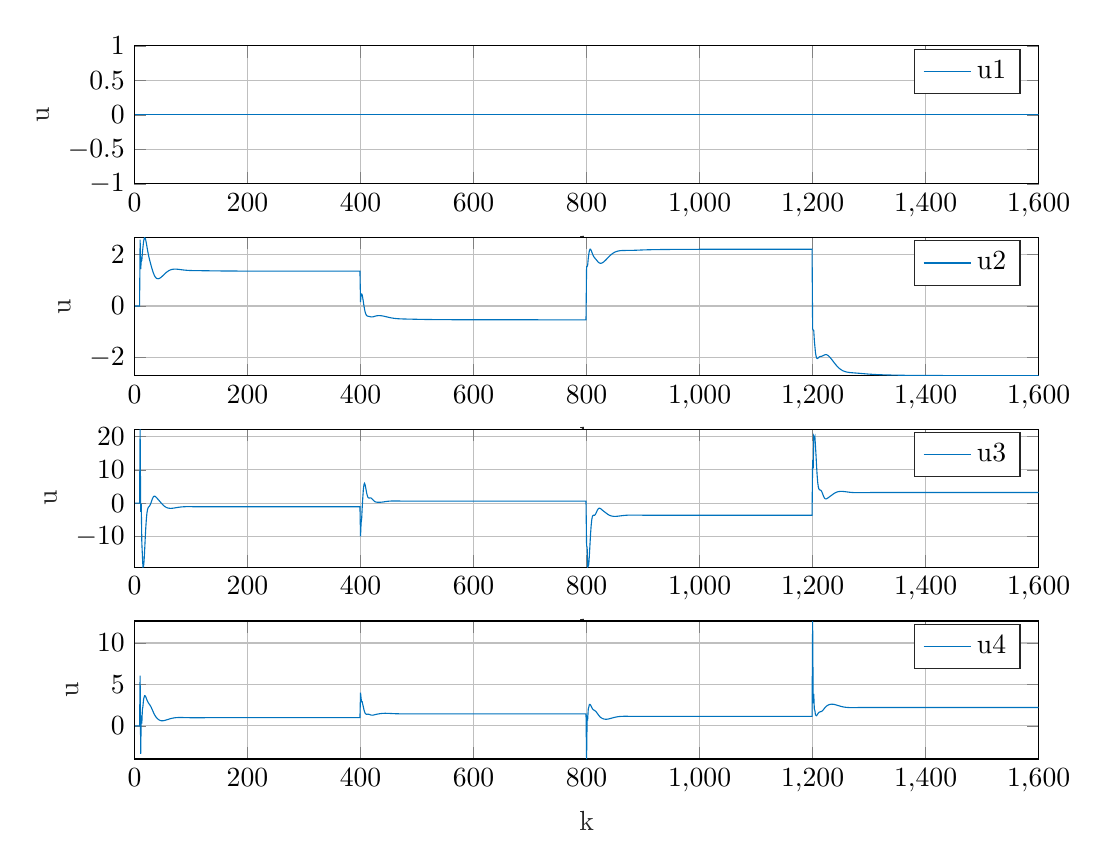
\begin{tikzpicture}

\begin{axis}[%
width=4.521in,
height=0.69in,
at={(0.758in,3.357in)},
scale only axis,
xmin=0,
xmax=1600,
xlabel style={font=\color{white!15!black}},
xlabel={k},
ymin=-1,
ymax=1,
ylabel style={font=\color{white!15!black}},
ylabel={u},
axis background/.style={fill=white},
xmajorgrids,
ymajorgrids,
legend style={legend cell align=left, align=left, draw=white!15!black}
]
\addplot [color=mycolor1]
  table[row sep=crcr]{%
1	0\\
2	0\\
3	0\\
4	0\\
5	0\\
6	0\\
7	0\\
8	0\\
9	0\\
10	0\\
11	0\\
12	0\\
13	0\\
14	0\\
15	0\\
16	0\\
17	0\\
18	0\\
19	0\\
20	0\\
21	0\\
22	0\\
23	0\\
24	0\\
25	0\\
26	0\\
27	0\\
28	0\\
29	0\\
30	0\\
31	0\\
32	0\\
33	0\\
34	0\\
35	0\\
36	0\\
37	0\\
38	0\\
39	0\\
40	0\\
41	0\\
42	0\\
43	0\\
44	0\\
45	0\\
46	0\\
47	0\\
48	0\\
49	0\\
50	0\\
51	0\\
52	0\\
53	0\\
54	0\\
55	0\\
56	0\\
57	0\\
58	0\\
59	0\\
60	0\\
61	0\\
62	0\\
63	0\\
64	0\\
65	0\\
66	0\\
67	0\\
68	0\\
69	0\\
70	0\\
71	0\\
72	0\\
73	0\\
74	0\\
75	0\\
76	0\\
77	0\\
78	0\\
79	0\\
80	0\\
81	0\\
82	0\\
83	0\\
84	0\\
85	0\\
86	0\\
87	0\\
88	0\\
89	0\\
90	0\\
91	0\\
92	0\\
93	0\\
94	0\\
95	0\\
96	0\\
97	0\\
98	0\\
99	0\\
100	0\\
101	0\\
102	0\\
103	0\\
104	0\\
105	0\\
106	0\\
107	0\\
108	0\\
109	0\\
110	0\\
111	0\\
112	0\\
113	0\\
114	0\\
115	0\\
116	0\\
117	0\\
118	0\\
119	0\\
120	0\\
121	0\\
122	0\\
123	0\\
124	0\\
125	0\\
126	0\\
127	0\\
128	0\\
129	0\\
130	0\\
131	0\\
132	0\\
133	0\\
134	0\\
135	0\\
136	0\\
137	0\\
138	0\\
139	0\\
140	0\\
141	0\\
142	0\\
143	0\\
144	0\\
145	0\\
146	0\\
147	0\\
148	0\\
149	0\\
150	0\\
151	0\\
152	0\\
153	0\\
154	0\\
155	0\\
156	0\\
157	0\\
158	0\\
159	0\\
160	0\\
161	0\\
162	0\\
163	0\\
164	0\\
165	0\\
166	0\\
167	0\\
168	0\\
169	0\\
170	0\\
171	0\\
172	0\\
173	0\\
174	0\\
175	0\\
176	0\\
177	0\\
178	0\\
179	0\\
180	0\\
181	0\\
182	0\\
183	0\\
184	0\\
185	0\\
186	0\\
187	0\\
188	0\\
189	0\\
190	0\\
191	0\\
192	0\\
193	0\\
194	0\\
195	0\\
196	0\\
197	0\\
198	0\\
199	0\\
200	0\\
201	0\\
202	0\\
203	0\\
204	0\\
205	0\\
206	0\\
207	0\\
208	0\\
209	0\\
210	0\\
211	0\\
212	0\\
213	0\\
214	0\\
215	0\\
216	0\\
217	0\\
218	0\\
219	0\\
220	0\\
221	0\\
222	0\\
223	0\\
224	0\\
225	0\\
226	0\\
227	0\\
228	0\\
229	0\\
230	0\\
231	0\\
232	0\\
233	0\\
234	0\\
235	0\\
236	0\\
237	0\\
238	0\\
239	0\\
240	0\\
241	0\\
242	0\\
243	0\\
244	0\\
245	0\\
246	0\\
247	0\\
248	0\\
249	0\\
250	0\\
251	0\\
252	0\\
253	0\\
254	0\\
255	0\\
256	0\\
257	0\\
258	0\\
259	0\\
260	0\\
261	0\\
262	0\\
263	0\\
264	0\\
265	0\\
266	0\\
267	0\\
268	0\\
269	0\\
270	0\\
271	0\\
272	0\\
273	0\\
274	0\\
275	0\\
276	0\\
277	0\\
278	0\\
279	0\\
280	0\\
281	0\\
282	0\\
283	0\\
284	0\\
285	0\\
286	0\\
287	0\\
288	0\\
289	0\\
290	0\\
291	0\\
292	0\\
293	0\\
294	0\\
295	0\\
296	0\\
297	0\\
298	0\\
299	0\\
300	0\\
301	0\\
302	0\\
303	0\\
304	0\\
305	0\\
306	0\\
307	0\\
308	0\\
309	0\\
310	0\\
311	0\\
312	0\\
313	0\\
314	0\\
315	0\\
316	0\\
317	0\\
318	0\\
319	0\\
320	0\\
321	0\\
322	0\\
323	0\\
324	0\\
325	0\\
326	0\\
327	0\\
328	0\\
329	0\\
330	0\\
331	0\\
332	0\\
333	0\\
334	0\\
335	0\\
336	0\\
337	0\\
338	0\\
339	0\\
340	0\\
341	0\\
342	0\\
343	0\\
344	0\\
345	0\\
346	0\\
347	0\\
348	0\\
349	0\\
350	0\\
351	0\\
352	0\\
353	0\\
354	0\\
355	0\\
356	0\\
357	0\\
358	0\\
359	0\\
360	0\\
361	0\\
362	0\\
363	0\\
364	0\\
365	0\\
366	0\\
367	0\\
368	0\\
369	0\\
370	0\\
371	0\\
372	0\\
373	0\\
374	0\\
375	0\\
376	0\\
377	0\\
378	0\\
379	0\\
380	0\\
381	0\\
382	0\\
383	0\\
384	0\\
385	0\\
386	0\\
387	0\\
388	0\\
389	0\\
390	0\\
391	0\\
392	0\\
393	0\\
394	0\\
395	0\\
396	0\\
397	0\\
398	0\\
399	0\\
400	0\\
401	0\\
402	0\\
403	0\\
404	0\\
405	0\\
406	0\\
407	0\\
408	0\\
409	0\\
410	0\\
411	0\\
412	0\\
413	0\\
414	0\\
415	0\\
416	0\\
417	0\\
418	0\\
419	0\\
420	0\\
421	0\\
422	0\\
423	0\\
424	0\\
425	0\\
426	0\\
427	0\\
428	0\\
429	0\\
430	0\\
431	0\\
432	0\\
433	0\\
434	0\\
435	0\\
436	0\\
437	0\\
438	0\\
439	0\\
440	0\\
441	0\\
442	0\\
443	0\\
444	0\\
445	0\\
446	0\\
447	0\\
448	0\\
449	0\\
450	0\\
451	0\\
452	0\\
453	0\\
454	0\\
455	0\\
456	0\\
457	0\\
458	0\\
459	0\\
460	0\\
461	0\\
462	0\\
463	0\\
464	0\\
465	0\\
466	0\\
467	0\\
468	0\\
469	0\\
470	0\\
471	0\\
472	0\\
473	0\\
474	0\\
475	0\\
476	0\\
477	0\\
478	0\\
479	0\\
480	0\\
481	0\\
482	0\\
483	0\\
484	0\\
485	0\\
486	0\\
487	0\\
488	0\\
489	0\\
490	0\\
491	0\\
492	0\\
493	0\\
494	0\\
495	0\\
496	0\\
497	0\\
498	0\\
499	0\\
500	0\\
501	0\\
502	0\\
503	0\\
504	0\\
505	0\\
506	0\\
507	0\\
508	0\\
509	0\\
510	0\\
511	0\\
512	0\\
513	0\\
514	0\\
515	0\\
516	0\\
517	0\\
518	0\\
519	0\\
520	0\\
521	0\\
522	0\\
523	0\\
524	0\\
525	0\\
526	0\\
527	0\\
528	0\\
529	0\\
530	0\\
531	0\\
532	0\\
533	0\\
534	0\\
535	0\\
536	0\\
537	0\\
538	0\\
539	0\\
540	0\\
541	0\\
542	0\\
543	0\\
544	0\\
545	0\\
546	0\\
547	0\\
548	0\\
549	0\\
550	0\\
551	0\\
552	0\\
553	0\\
554	0\\
555	0\\
556	0\\
557	0\\
558	0\\
559	0\\
560	0\\
561	0\\
562	0\\
563	0\\
564	0\\
565	0\\
566	0\\
567	0\\
568	0\\
569	0\\
570	0\\
571	0\\
572	0\\
573	0\\
574	0\\
575	0\\
576	0\\
577	0\\
578	0\\
579	0\\
580	0\\
581	0\\
582	0\\
583	0\\
584	0\\
585	0\\
586	0\\
587	0\\
588	0\\
589	0\\
590	0\\
591	0\\
592	0\\
593	0\\
594	0\\
595	0\\
596	0\\
597	0\\
598	0\\
599	0\\
600	0\\
601	0\\
602	0\\
603	0\\
604	0\\
605	0\\
606	0\\
607	0\\
608	0\\
609	0\\
610	0\\
611	0\\
612	0\\
613	0\\
614	0\\
615	0\\
616	0\\
617	0\\
618	0\\
619	0\\
620	0\\
621	0\\
622	0\\
623	0\\
624	0\\
625	0\\
626	0\\
627	0\\
628	0\\
629	0\\
630	0\\
631	0\\
632	0\\
633	0\\
634	0\\
635	0\\
636	0\\
637	0\\
638	0\\
639	0\\
640	0\\
641	0\\
642	0\\
643	0\\
644	0\\
645	0\\
646	0\\
647	0\\
648	0\\
649	0\\
650	0\\
651	0\\
652	0\\
653	0\\
654	0\\
655	0\\
656	0\\
657	0\\
658	0\\
659	0\\
660	0\\
661	0\\
662	0\\
663	0\\
664	0\\
665	0\\
666	0\\
667	0\\
668	0\\
669	0\\
670	0\\
671	0\\
672	0\\
673	0\\
674	0\\
675	0\\
676	0\\
677	0\\
678	0\\
679	0\\
680	0\\
681	0\\
682	0\\
683	0\\
684	0\\
685	0\\
686	0\\
687	0\\
688	0\\
689	0\\
690	0\\
691	0\\
692	0\\
693	0\\
694	0\\
695	0\\
696	0\\
697	0\\
698	0\\
699	0\\
700	0\\
701	0\\
702	0\\
703	0\\
704	0\\
705	0\\
706	0\\
707	0\\
708	0\\
709	0\\
710	0\\
711	0\\
712	0\\
713	0\\
714	0\\
715	0\\
716	0\\
717	0\\
718	0\\
719	0\\
720	0\\
721	0\\
722	0\\
723	0\\
724	0\\
725	0\\
726	0\\
727	0\\
728	0\\
729	0\\
730	0\\
731	0\\
732	0\\
733	0\\
734	0\\
735	0\\
736	0\\
737	0\\
738	0\\
739	0\\
740	0\\
741	0\\
742	0\\
743	0\\
744	0\\
745	0\\
746	0\\
747	0\\
748	0\\
749	0\\
750	0\\
751	0\\
752	0\\
753	0\\
754	0\\
755	0\\
756	0\\
757	0\\
758	0\\
759	0\\
760	0\\
761	0\\
762	0\\
763	0\\
764	0\\
765	0\\
766	0\\
767	0\\
768	0\\
769	0\\
770	0\\
771	0\\
772	0\\
773	0\\
774	0\\
775	0\\
776	0\\
777	0\\
778	0\\
779	0\\
780	0\\
781	0\\
782	0\\
783	0\\
784	0\\
785	0\\
786	0\\
787	0\\
788	0\\
789	0\\
790	0\\
791	0\\
792	0\\
793	0\\
794	0\\
795	0\\
796	0\\
797	0\\
798	0\\
799	0\\
800	0\\
801	0\\
802	0\\
803	0\\
804	0\\
805	0\\
806	0\\
807	0\\
808	0\\
809	0\\
810	0\\
811	0\\
812	0\\
813	0\\
814	0\\
815	0\\
816	0\\
817	0\\
818	0\\
819	0\\
820	0\\
821	0\\
822	0\\
823	0\\
824	0\\
825	0\\
826	0\\
827	0\\
828	0\\
829	0\\
830	0\\
831	0\\
832	0\\
833	0\\
834	0\\
835	0\\
836	0\\
837	0\\
838	0\\
839	0\\
840	0\\
841	0\\
842	0\\
843	0\\
844	0\\
845	0\\
846	0\\
847	0\\
848	0\\
849	0\\
850	0\\
851	0\\
852	0\\
853	0\\
854	0\\
855	0\\
856	0\\
857	0\\
858	0\\
859	0\\
860	0\\
861	0\\
862	0\\
863	0\\
864	0\\
865	0\\
866	0\\
867	0\\
868	0\\
869	0\\
870	0\\
871	0\\
872	0\\
873	0\\
874	0\\
875	0\\
876	0\\
877	0\\
878	0\\
879	0\\
880	0\\
881	0\\
882	0\\
883	0\\
884	0\\
885	0\\
886	0\\
887	0\\
888	0\\
889	0\\
890	0\\
891	0\\
892	0\\
893	0\\
894	0\\
895	0\\
896	0\\
897	0\\
898	0\\
899	0\\
900	0\\
901	0\\
902	0\\
903	0\\
904	0\\
905	0\\
906	0\\
907	0\\
908	0\\
909	0\\
910	0\\
911	0\\
912	0\\
913	0\\
914	0\\
915	0\\
916	0\\
917	0\\
918	0\\
919	0\\
920	0\\
921	0\\
922	0\\
923	0\\
924	0\\
925	0\\
926	0\\
927	0\\
928	0\\
929	0\\
930	0\\
931	0\\
932	0\\
933	0\\
934	0\\
935	0\\
936	0\\
937	0\\
938	0\\
939	0\\
940	0\\
941	0\\
942	0\\
943	0\\
944	0\\
945	0\\
946	0\\
947	0\\
948	0\\
949	0\\
950	0\\
951	0\\
952	0\\
953	0\\
954	0\\
955	0\\
956	0\\
957	0\\
958	0\\
959	0\\
960	0\\
961	0\\
962	0\\
963	0\\
964	0\\
965	0\\
966	0\\
967	0\\
968	0\\
969	0\\
970	0\\
971	0\\
972	0\\
973	0\\
974	0\\
975	0\\
976	0\\
977	0\\
978	0\\
979	0\\
980	0\\
981	0\\
982	0\\
983	0\\
984	0\\
985	0\\
986	0\\
987	0\\
988	0\\
989	0\\
990	0\\
991	0\\
992	0\\
993	0\\
994	0\\
995	0\\
996	0\\
997	0\\
998	0\\
999	0\\
1000	0\\
1001	0\\
1002	0\\
1003	0\\
1004	0\\
1005	0\\
1006	0\\
1007	0\\
1008	0\\
1009	0\\
1010	0\\
1011	0\\
1012	0\\
1013	0\\
1014	0\\
1015	0\\
1016	0\\
1017	0\\
1018	0\\
1019	0\\
1020	0\\
1021	0\\
1022	0\\
1023	0\\
1024	0\\
1025	0\\
1026	0\\
1027	0\\
1028	0\\
1029	0\\
1030	0\\
1031	0\\
1032	0\\
1033	0\\
1034	0\\
1035	0\\
1036	0\\
1037	0\\
1038	0\\
1039	0\\
1040	0\\
1041	0\\
1042	0\\
1043	0\\
1044	0\\
1045	0\\
1046	0\\
1047	0\\
1048	0\\
1049	0\\
1050	0\\
1051	0\\
1052	0\\
1053	0\\
1054	0\\
1055	0\\
1056	0\\
1057	0\\
1058	0\\
1059	0\\
1060	0\\
1061	0\\
1062	0\\
1063	0\\
1064	0\\
1065	0\\
1066	0\\
1067	0\\
1068	0\\
1069	0\\
1070	0\\
1071	0\\
1072	0\\
1073	0\\
1074	0\\
1075	0\\
1076	0\\
1077	0\\
1078	0\\
1079	0\\
1080	0\\
1081	0\\
1082	0\\
1083	0\\
1084	0\\
1085	0\\
1086	0\\
1087	0\\
1088	0\\
1089	0\\
1090	0\\
1091	0\\
1092	0\\
1093	0\\
1094	0\\
1095	0\\
1096	0\\
1097	0\\
1098	0\\
1099	0\\
1100	0\\
1101	0\\
1102	0\\
1103	0\\
1104	0\\
1105	0\\
1106	0\\
1107	0\\
1108	0\\
1109	0\\
1110	0\\
1111	0\\
1112	0\\
1113	0\\
1114	0\\
1115	0\\
1116	0\\
1117	0\\
1118	0\\
1119	0\\
1120	0\\
1121	0\\
1122	0\\
1123	0\\
1124	0\\
1125	0\\
1126	0\\
1127	0\\
1128	0\\
1129	0\\
1130	0\\
1131	0\\
1132	0\\
1133	0\\
1134	0\\
1135	0\\
1136	0\\
1137	0\\
1138	0\\
1139	0\\
1140	0\\
1141	0\\
1142	0\\
1143	0\\
1144	0\\
1145	0\\
1146	0\\
1147	0\\
1148	0\\
1149	0\\
1150	0\\
1151	0\\
1152	0\\
1153	0\\
1154	0\\
1155	0\\
1156	0\\
1157	0\\
1158	0\\
1159	0\\
1160	0\\
1161	0\\
1162	0\\
1163	0\\
1164	0\\
1165	0\\
1166	0\\
1167	0\\
1168	0\\
1169	0\\
1170	0\\
1171	0\\
1172	0\\
1173	0\\
1174	0\\
1175	0\\
1176	0\\
1177	0\\
1178	0\\
1179	0\\
1180	0\\
1181	0\\
1182	0\\
1183	0\\
1184	0\\
1185	0\\
1186	0\\
1187	0\\
1188	0\\
1189	0\\
1190	0\\
1191	0\\
1192	0\\
1193	0\\
1194	0\\
1195	0\\
1196	0\\
1197	0\\
1198	0\\
1199	0\\
1200	0\\
1201	0\\
1202	0\\
1203	0\\
1204	0\\
1205	0\\
1206	0\\
1207	0\\
1208	0\\
1209	0\\
1210	0\\
1211	0\\
1212	0\\
1213	0\\
1214	0\\
1215	0\\
1216	0\\
1217	0\\
1218	0\\
1219	0\\
1220	0\\
1221	0\\
1222	0\\
1223	0\\
1224	0\\
1225	0\\
1226	0\\
1227	0\\
1228	0\\
1229	0\\
1230	0\\
1231	0\\
1232	0\\
1233	0\\
1234	0\\
1235	0\\
1236	0\\
1237	0\\
1238	0\\
1239	0\\
1240	0\\
1241	0\\
1242	0\\
1243	0\\
1244	0\\
1245	0\\
1246	0\\
1247	0\\
1248	0\\
1249	0\\
1250	0\\
1251	0\\
1252	0\\
1253	0\\
1254	0\\
1255	0\\
1256	0\\
1257	0\\
1258	0\\
1259	0\\
1260	0\\
1261	0\\
1262	0\\
1263	0\\
1264	0\\
1265	0\\
1266	0\\
1267	0\\
1268	0\\
1269	0\\
1270	0\\
1271	0\\
1272	0\\
1273	0\\
1274	0\\
1275	0\\
1276	0\\
1277	0\\
1278	0\\
1279	0\\
1280	0\\
1281	0\\
1282	0\\
1283	0\\
1284	0\\
1285	0\\
1286	0\\
1287	0\\
1288	0\\
1289	0\\
1290	0\\
1291	0\\
1292	0\\
1293	0\\
1294	0\\
1295	0\\
1296	0\\
1297	0\\
1298	0\\
1299	0\\
1300	0\\
1301	0\\
1302	0\\
1303	0\\
1304	0\\
1305	0\\
1306	0\\
1307	0\\
1308	0\\
1309	0\\
1310	0\\
1311	0\\
1312	0\\
1313	0\\
1314	0\\
1315	0\\
1316	0\\
1317	0\\
1318	0\\
1319	0\\
1320	0\\
1321	0\\
1322	0\\
1323	0\\
1324	0\\
1325	0\\
1326	0\\
1327	0\\
1328	0\\
1329	0\\
1330	0\\
1331	0\\
1332	0\\
1333	0\\
1334	0\\
1335	0\\
1336	0\\
1337	0\\
1338	0\\
1339	0\\
1340	0\\
1341	0\\
1342	0\\
1343	0\\
1344	0\\
1345	0\\
1346	0\\
1347	0\\
1348	0\\
1349	0\\
1350	0\\
1351	0\\
1352	0\\
1353	0\\
1354	0\\
1355	0\\
1356	0\\
1357	0\\
1358	0\\
1359	0\\
1360	0\\
1361	0\\
1362	0\\
1363	0\\
1364	0\\
1365	0\\
1366	0\\
1367	0\\
1368	0\\
1369	0\\
1370	0\\
1371	0\\
1372	0\\
1373	0\\
1374	0\\
1375	0\\
1376	0\\
1377	0\\
1378	0\\
1379	0\\
1380	0\\
1381	0\\
1382	0\\
1383	0\\
1384	0\\
1385	0\\
1386	0\\
1387	0\\
1388	0\\
1389	0\\
1390	0\\
1391	0\\
1392	0\\
1393	0\\
1394	0\\
1395	0\\
1396	0\\
1397	0\\
1398	0\\
1399	0\\
1400	0\\
1401	0\\
1402	0\\
1403	0\\
1404	0\\
1405	0\\
1406	0\\
1407	0\\
1408	0\\
1409	0\\
1410	0\\
1411	0\\
1412	0\\
1413	0\\
1414	0\\
1415	0\\
1416	0\\
1417	0\\
1418	0\\
1419	0\\
1420	0\\
1421	0\\
1422	0\\
1423	0\\
1424	0\\
1425	0\\
1426	0\\
1427	0\\
1428	0\\
1429	0\\
1430	0\\
1431	0\\
1432	0\\
1433	0\\
1434	0\\
1435	0\\
1436	0\\
1437	0\\
1438	0\\
1439	0\\
1440	0\\
1441	0\\
1442	0\\
1443	0\\
1444	0\\
1445	0\\
1446	0\\
1447	0\\
1448	0\\
1449	0\\
1450	0\\
1451	0\\
1452	0\\
1453	0\\
1454	0\\
1455	0\\
1456	0\\
1457	0\\
1458	0\\
1459	0\\
1460	0\\
1461	0\\
1462	0\\
1463	0\\
1464	0\\
1465	0\\
1466	0\\
1467	0\\
1468	0\\
1469	0\\
1470	0\\
1471	0\\
1472	0\\
1473	0\\
1474	0\\
1475	0\\
1476	0\\
1477	0\\
1478	0\\
1479	0\\
1480	0\\
1481	0\\
1482	0\\
1483	0\\
1484	0\\
1485	0\\
1486	0\\
1487	0\\
1488	0\\
1489	0\\
1490	0\\
1491	0\\
1492	0\\
1493	0\\
1494	0\\
1495	0\\
1496	0\\
1497	0\\
1498	0\\
1499	0\\
1500	0\\
1501	0\\
1502	0\\
1503	0\\
1504	0\\
1505	0\\
1506	0\\
1507	0\\
1508	0\\
1509	0\\
1510	0\\
1511	0\\
1512	0\\
1513	0\\
1514	0\\
1515	0\\
1516	0\\
1517	0\\
1518	0\\
1519	0\\
1520	0\\
1521	0\\
1522	0\\
1523	0\\
1524	0\\
1525	0\\
1526	0\\
1527	0\\
1528	0\\
1529	0\\
1530	0\\
1531	0\\
1532	0\\
1533	0\\
1534	0\\
1535	0\\
1536	0\\
1537	0\\
1538	0\\
1539	0\\
1540	0\\
1541	0\\
1542	0\\
1543	0\\
1544	0\\
1545	0\\
1546	0\\
1547	0\\
1548	0\\
1549	0\\
1550	0\\
1551	0\\
1552	0\\
1553	0\\
1554	0\\
1555	0\\
1556	0\\
1557	0\\
1558	0\\
1559	0\\
1560	0\\
1561	0\\
1562	0\\
1563	0\\
1564	0\\
1565	0\\
1566	0\\
1567	0\\
1568	0\\
1569	0\\
1570	0\\
1571	0\\
1572	0\\
1573	0\\
1574	0\\
1575	0\\
1576	0\\
1577	0\\
1578	0\\
1579	0\\
1580	0\\
1581	0\\
1582	0\\
1583	0\\
1584	0\\
1585	0\\
1586	0\\
1587	0\\
1588	0\\
1589	0\\
1590	0\\
1591	0\\
1592	0\\
1593	0\\
1594	0\\
1595	0\\
1596	0\\
1597	0\\
1598	0\\
1599	0\\
1600	0\\
};
\addlegendentry{u1}

\end{axis}

\begin{axis}[%
width=4.521in,
height=0.69in,
at={(0.758in,2.398in)},
scale only axis,
xmin=0,
xmax=1600,
xlabel style={font=\color{white!15!black}},
xlabel={k},
ymin=-2.7028,
ymax=2.6543,
ylabel style={font=\color{white!15!black}},
ylabel={u},
axis background/.style={fill=white},
xmajorgrids,
ymajorgrids,
legend style={legend cell align=left, align=left, draw=white!15!black}
]
\addplot [color=mycolor1]
  table[row sep=crcr]{%
1	0\\
2	0\\
3	0\\
4	0\\
5	0\\
6	0\\
7	0\\
8	0\\
9	0\\
10	2.5762\\
11	1.4334\\
12	1.7475\\
13	1.7623\\
14	2.0627\\
15	2.2759\\
16	2.4855\\
17	2.6054\\
18	2.6543\\
19	2.6286\\
20	2.5507\\
21	2.4386\\
22	2.3121\\
23	2.1845\\
24	2.0647\\
25	1.9559\\
26	1.8577\\
27	1.7679\\
28	1.6837\\
29	1.603\\
30	1.5248\\
31	1.4491\\
32	1.3772\\
33	1.3104\\
34	1.2504\\
35	1.1984\\
36	1.155\\
37	1.1205\\
38	1.0944\\
39	1.0761\\
40	1.0648\\
41	1.0596\\
42	1.0595\\
43	1.0639\\
44	1.072\\
45	1.0833\\
46	1.0974\\
47	1.1137\\
48	1.1319\\
49	1.1515\\
50	1.1722\\
51	1.1934\\
52	1.2148\\
53	1.2361\\
54	1.2568\\
55	1.2769\\
56	1.2961\\
57	1.3141\\
58	1.3309\\
59	1.3464\\
60	1.3605\\
61	1.3733\\
62	1.3846\\
63	1.3946\\
64	1.4032\\
65	1.4106\\
66	1.4167\\
67	1.4216\\
68	1.4254\\
69	1.4282\\
70	1.43\\
71	1.4311\\
72	1.4313\\
73	1.431\\
74	1.43\\
75	1.4286\\
76	1.4267\\
77	1.4246\\
78	1.4221\\
79	1.4195\\
80	1.4167\\
81	1.4139\\
82	1.411\\
83	1.4081\\
84	1.4053\\
85	1.4025\\
86	1.3998\\
87	1.3972\\
88	1.3948\\
89	1.3924\\
90	1.3903\\
91	1.3883\\
92	1.3864\\
93	1.3847\\
94	1.3832\\
95	1.3817\\
96	1.3805\\
97	1.3793\\
98	1.3783\\
99	1.3774\\
100	1.3766\\
101	1.3759\\
102	1.3753\\
103	1.3747\\
104	1.3742\\
105	1.3738\\
106	1.3734\\
107	1.3731\\
108	1.3728\\
109	1.3725\\
110	1.3722\\
111	1.372\\
112	1.3717\\
113	1.3715\\
114	1.3713\\
115	1.371\\
116	1.3708\\
117	1.3706\\
118	1.3703\\
119	1.3701\\
120	1.3698\\
121	1.3695\\
122	1.3692\\
123	1.369\\
124	1.3687\\
125	1.3684\\
126	1.368\\
127	1.3677\\
128	1.3674\\
129	1.3671\\
130	1.3668\\
131	1.3664\\
132	1.3661\\
133	1.3658\\
134	1.3655\\
135	1.3651\\
136	1.3648\\
137	1.3645\\
138	1.3642\\
139	1.3639\\
140	1.3636\\
141	1.3633\\
142	1.363\\
143	1.3627\\
144	1.3625\\
145	1.3622\\
146	1.3619\\
147	1.3617\\
148	1.3614\\
149	1.3612\\
150	1.361\\
151	1.3607\\
152	1.3605\\
153	1.3603\\
154	1.3601\\
155	1.3599\\
156	1.3597\\
157	1.3596\\
158	1.3594\\
159	1.3592\\
160	1.359\\
161	1.3589\\
162	1.3587\\
163	1.3586\\
164	1.3584\\
165	1.3583\\
166	1.3581\\
167	1.358\\
168	1.3579\\
169	1.3577\\
170	1.3576\\
171	1.3575\\
172	1.3574\\
173	1.3572\\
174	1.3571\\
175	1.357\\
176	1.3569\\
177	1.3568\\
178	1.3567\\
179	1.3566\\
180	1.3565\\
181	1.3564\\
182	1.3563\\
183	1.3562\\
184	1.3561\\
185	1.356\\
186	1.356\\
187	1.3559\\
188	1.3558\\
189	1.3557\\
190	1.3556\\
191	1.3555\\
192	1.3555\\
193	1.3554\\
194	1.3553\\
195	1.3553\\
196	1.3552\\
197	1.3551\\
198	1.3551\\
199	1.355\\
200	1.3549\\
201	1.3549\\
202	1.3548\\
203	1.3548\\
204	1.3547\\
205	1.3546\\
206	1.3546\\
207	1.3545\\
208	1.3545\\
209	1.3544\\
210	1.3544\\
211	1.3543\\
212	1.3543\\
213	1.3543\\
214	1.3542\\
215	1.3542\\
216	1.3541\\
217	1.3541\\
218	1.354\\
219	1.354\\
220	1.354\\
221	1.3539\\
222	1.3539\\
223	1.3539\\
224	1.3538\\
225	1.3538\\
226	1.3538\\
227	1.3537\\
228	1.3537\\
229	1.3537\\
230	1.3536\\
231	1.3536\\
232	1.3536\\
233	1.3536\\
234	1.3535\\
235	1.3535\\
236	1.3535\\
237	1.3535\\
238	1.3534\\
239	1.3534\\
240	1.3534\\
241	1.3534\\
242	1.3533\\
243	1.3533\\
244	1.3533\\
245	1.3533\\
246	1.3533\\
247	1.3532\\
248	1.3532\\
249	1.3532\\
250	1.3532\\
251	1.3532\\
252	1.3532\\
253	1.3531\\
254	1.3531\\
255	1.3531\\
256	1.3531\\
257	1.3531\\
258	1.3531\\
259	1.353\\
260	1.353\\
261	1.353\\
262	1.353\\
263	1.353\\
264	1.353\\
265	1.353\\
266	1.353\\
267	1.3529\\
268	1.3529\\
269	1.3529\\
270	1.3529\\
271	1.3529\\
272	1.3529\\
273	1.3529\\
274	1.3529\\
275	1.3529\\
276	1.3528\\
277	1.3528\\
278	1.3528\\
279	1.3528\\
280	1.3528\\
281	1.3528\\
282	1.3528\\
283	1.3528\\
284	1.3528\\
285	1.3528\\
286	1.3528\\
287	1.3528\\
288	1.3528\\
289	1.3527\\
290	1.3527\\
291	1.3527\\
292	1.3527\\
293	1.3527\\
294	1.3527\\
295	1.3527\\
296	1.3527\\
297	1.3527\\
298	1.3527\\
299	1.3527\\
300	1.3527\\
301	1.3527\\
302	1.3527\\
303	1.3527\\
304	1.3527\\
305	1.3527\\
306	1.3527\\
307	1.3527\\
308	1.3526\\
309	1.3526\\
310	1.3526\\
311	1.3526\\
312	1.3526\\
313	1.3526\\
314	1.3526\\
315	1.3526\\
316	1.3526\\
317	1.3526\\
318	1.3526\\
319	1.3526\\
320	1.3526\\
321	1.3526\\
322	1.3526\\
323	1.3526\\
324	1.3526\\
325	1.3526\\
326	1.3526\\
327	1.3526\\
328	1.3526\\
329	1.3526\\
330	1.3526\\
331	1.3526\\
332	1.3526\\
333	1.3526\\
334	1.3526\\
335	1.3526\\
336	1.3526\\
337	1.3526\\
338	1.3526\\
339	1.3526\\
340	1.3526\\
341	1.3526\\
342	1.3526\\
343	1.3525\\
344	1.3525\\
345	1.3525\\
346	1.3525\\
347	1.3525\\
348	1.3525\\
349	1.3525\\
350	1.3525\\
351	1.3525\\
352	1.3525\\
353	1.3525\\
354	1.3525\\
355	1.3525\\
356	1.3525\\
357	1.3525\\
358	1.3525\\
359	1.3525\\
360	1.3525\\
361	1.3525\\
362	1.3525\\
363	1.3525\\
364	1.3525\\
365	1.3525\\
366	1.3525\\
367	1.3525\\
368	1.3525\\
369	1.3525\\
370	1.3525\\
371	1.3525\\
372	1.3525\\
373	1.3525\\
374	1.3525\\
375	1.3525\\
376	1.3525\\
377	1.3525\\
378	1.3525\\
379	1.3525\\
380	1.3525\\
381	1.3525\\
382	1.3525\\
383	1.3525\\
384	1.3525\\
385	1.3525\\
386	1.3525\\
387	1.3525\\
388	1.3525\\
389	1.3525\\
390	1.3525\\
391	1.3525\\
392	1.3525\\
393	1.3525\\
394	1.3525\\
395	1.3525\\
396	1.3525\\
397	1.3525\\
398	1.3525\\
399	1.3525\\
400	0.15025\\
401	0.46918\\
402	0.46953\\
403	0.42304\\
404	0.30264\\
405	0.16359\\
406	0.017807\\
407	-0.11177\\
408	-0.217\\
409	-0.29345\\
410	-0.3437\\
411	-0.37308\\
412	-0.38845\\
413	-0.39604\\
414	-0.40058\\
415	-0.40485\\
416	-0.40986\\
417	-0.41536\\
418	-0.42042\\
419	-0.42402\\
420	-0.42539\\
421	-0.42421\\
422	-0.42064\\
423	-0.4152\\
424	-0.4086\\
425	-0.4016\\
426	-0.39484\\
427	-0.3888\\
428	-0.38376\\
429	-0.37983\\
430	-0.37701\\
431	-0.3752\\
432	-0.37428\\
433	-0.37414\\
434	-0.37471\\
435	-0.37593\\
436	-0.37776\\
437	-0.38018\\
438	-0.38315\\
439	-0.38665\\
440	-0.39062\\
441	-0.395\\
442	-0.39973\\
443	-0.40472\\
444	-0.4099\\
445	-0.4152\\
446	-0.42055\\
447	-0.42588\\
448	-0.43117\\
449	-0.43636\\
450	-0.44141\\
451	-0.44631\\
452	-0.45103\\
453	-0.45555\\
454	-0.45986\\
455	-0.46393\\
456	-0.46777\\
457	-0.47137\\
458	-0.47473\\
459	-0.47786\\
460	-0.48074\\
461	-0.4834\\
462	-0.48584\\
463	-0.48808\\
464	-0.49012\\
465	-0.49198\\
466	-0.49366\\
467	-0.4952\\
468	-0.49658\\
469	-0.49784\\
470	-0.49899\\
471	-0.50003\\
472	-0.50097\\
473	-0.50184\\
474	-0.50264\\
475	-0.50338\\
476	-0.50406\\
477	-0.50471\\
478	-0.50532\\
479	-0.5059\\
480	-0.50646\\
481	-0.507\\
482	-0.50753\\
483	-0.50805\\
484	-0.50856\\
485	-0.50907\\
486	-0.50958\\
487	-0.51008\\
488	-0.51059\\
489	-0.5111\\
490	-0.51161\\
491	-0.51212\\
492	-0.51263\\
493	-0.51314\\
494	-0.51365\\
495	-0.51417\\
496	-0.51468\\
497	-0.51518\\
498	-0.51569\\
499	-0.51619\\
500	-0.51668\\
501	-0.51717\\
502	-0.51765\\
503	-0.51813\\
504	-0.5186\\
505	-0.51905\\
506	-0.5195\\
507	-0.51994\\
508	-0.52037\\
509	-0.52079\\
510	-0.5212\\
511	-0.5216\\
512	-0.52199\\
513	-0.52236\\
514	-0.52273\\
515	-0.52308\\
516	-0.52343\\
517	-0.52376\\
518	-0.52409\\
519	-0.5244\\
520	-0.52471\\
521	-0.525\\
522	-0.52529\\
523	-0.52557\\
524	-0.52584\\
525	-0.5261\\
526	-0.52635\\
527	-0.5266\\
528	-0.52684\\
529	-0.52707\\
530	-0.5273\\
531	-0.52752\\
532	-0.52773\\
533	-0.52794\\
534	-0.52814\\
535	-0.52834\\
536	-0.52853\\
537	-0.52872\\
538	-0.5289\\
539	-0.52908\\
540	-0.52925\\
541	-0.52942\\
542	-0.52959\\
543	-0.52975\\
544	-0.52991\\
545	-0.53006\\
546	-0.53021\\
547	-0.53036\\
548	-0.5305\\
549	-0.53065\\
550	-0.53078\\
551	-0.53092\\
552	-0.53105\\
553	-0.53118\\
554	-0.5313\\
555	-0.53143\\
556	-0.53155\\
557	-0.53166\\
558	-0.53178\\
559	-0.53189\\
560	-0.532\\
561	-0.5321\\
562	-0.53221\\
563	-0.53231\\
564	-0.53241\\
565	-0.53251\\
566	-0.5326\\
567	-0.53269\\
568	-0.53278\\
569	-0.53287\\
570	-0.53295\\
571	-0.53304\\
572	-0.53312\\
573	-0.5332\\
574	-0.53328\\
575	-0.53335\\
576	-0.53343\\
577	-0.5335\\
578	-0.53357\\
579	-0.53364\\
580	-0.5337\\
581	-0.53377\\
582	-0.53383\\
583	-0.53389\\
584	-0.53395\\
585	-0.53401\\
586	-0.53407\\
587	-0.53412\\
588	-0.53418\\
589	-0.53423\\
590	-0.53428\\
591	-0.53434\\
592	-0.53438\\
593	-0.53443\\
594	-0.53448\\
595	-0.53453\\
596	-0.53457\\
597	-0.53461\\
598	-0.53466\\
599	-0.5347\\
600	-0.53474\\
601	-0.53478\\
602	-0.53482\\
603	-0.53485\\
604	-0.53489\\
605	-0.53493\\
606	-0.53496\\
607	-0.535\\
608	-0.53503\\
609	-0.53506\\
610	-0.53509\\
611	-0.53512\\
612	-0.53516\\
613	-0.53518\\
614	-0.53521\\
615	-0.53524\\
616	-0.53527\\
617	-0.5353\\
618	-0.53532\\
619	-0.53535\\
620	-0.53537\\
621	-0.5354\\
622	-0.53542\\
623	-0.53544\\
624	-0.53546\\
625	-0.53549\\
626	-0.53551\\
627	-0.53553\\
628	-0.53555\\
629	-0.53557\\
630	-0.53559\\
631	-0.53561\\
632	-0.53563\\
633	-0.53564\\
634	-0.53566\\
635	-0.53568\\
636	-0.53569\\
637	-0.53571\\
638	-0.53573\\
639	-0.53574\\
640	-0.53576\\
641	-0.53577\\
642	-0.53579\\
643	-0.5358\\
644	-0.53581\\
645	-0.53583\\
646	-0.53584\\
647	-0.53585\\
648	-0.53587\\
649	-0.53588\\
650	-0.53589\\
651	-0.5359\\
652	-0.53591\\
653	-0.53592\\
654	-0.53593\\
655	-0.53594\\
656	-0.53595\\
657	-0.53596\\
658	-0.53597\\
659	-0.53598\\
660	-0.53599\\
661	-0.536\\
662	-0.53601\\
663	-0.53602\\
664	-0.53603\\
665	-0.53604\\
666	-0.53604\\
667	-0.53605\\
668	-0.53606\\
669	-0.53607\\
670	-0.53607\\
671	-0.53608\\
672	-0.53609\\
673	-0.53609\\
674	-0.5361\\
675	-0.53611\\
676	-0.53611\\
677	-0.53612\\
678	-0.53612\\
679	-0.53613\\
680	-0.53614\\
681	-0.53614\\
682	-0.53615\\
683	-0.53615\\
684	-0.53616\\
685	-0.53616\\
686	-0.53617\\
687	-0.53617\\
688	-0.53618\\
689	-0.53618\\
690	-0.53619\\
691	-0.53619\\
692	-0.53619\\
693	-0.5362\\
694	-0.5362\\
695	-0.53621\\
696	-0.53621\\
697	-0.53621\\
698	-0.53622\\
699	-0.53622\\
700	-0.53622\\
701	-0.53623\\
702	-0.53623\\
703	-0.53623\\
704	-0.53624\\
705	-0.53624\\
706	-0.53624\\
707	-0.53624\\
708	-0.53625\\
709	-0.53625\\
710	-0.53625\\
711	-0.53626\\
712	-0.53626\\
713	-0.53626\\
714	-0.53626\\
715	-0.53627\\
716	-0.53627\\
717	-0.53627\\
718	-0.53627\\
719	-0.53627\\
720	-0.53628\\
721	-0.53628\\
722	-0.53628\\
723	-0.53628\\
724	-0.53628\\
725	-0.53629\\
726	-0.53629\\
727	-0.53629\\
728	-0.53629\\
729	-0.53629\\
730	-0.53629\\
731	-0.5363\\
732	-0.5363\\
733	-0.5363\\
734	-0.5363\\
735	-0.5363\\
736	-0.5363\\
737	-0.53631\\
738	-0.53631\\
739	-0.53631\\
740	-0.53631\\
741	-0.53631\\
742	-0.53631\\
743	-0.53631\\
744	-0.53631\\
745	-0.53631\\
746	-0.53632\\
747	-0.53632\\
748	-0.53632\\
749	-0.53632\\
750	-0.53632\\
751	-0.53632\\
752	-0.53632\\
753	-0.53632\\
754	-0.53632\\
755	-0.53632\\
756	-0.53633\\
757	-0.53633\\
758	-0.53633\\
759	-0.53633\\
760	-0.53633\\
761	-0.53633\\
762	-0.53633\\
763	-0.53633\\
764	-0.53633\\
765	-0.53633\\
766	-0.53633\\
767	-0.53633\\
768	-0.53633\\
769	-0.53633\\
770	-0.53634\\
771	-0.53634\\
772	-0.53634\\
773	-0.53634\\
774	-0.53634\\
775	-0.53634\\
776	-0.53634\\
777	-0.53634\\
778	-0.53634\\
779	-0.53634\\
780	-0.53634\\
781	-0.53634\\
782	-0.53634\\
783	-0.53634\\
784	-0.53634\\
785	-0.53634\\
786	-0.53634\\
787	-0.53634\\
788	-0.53634\\
789	-0.53634\\
790	-0.53634\\
791	-0.53635\\
792	-0.53635\\
793	-0.53635\\
794	-0.53635\\
795	-0.53635\\
796	-0.53635\\
797	-0.53635\\
798	-0.53635\\
799	-0.53635\\
800	1.5247\\
801	1.5302\\
802	1.6066\\
803	1.8568\\
804	2.0218\\
805	2.1499\\
806	2.2016\\
807	2.2036\\
808	2.1663\\
809	2.1109\\
810	2.0502\\
811	1.9943\\
812	1.947\\
813	1.9089\\
814	1.8777\\
815	1.8504\\
816	1.8246\\
817	1.7986\\
818	1.7719\\
819	1.7454\\
820	1.7203\\
821	1.6981\\
822	1.68\\
823	1.667\\
824	1.6594\\
825	1.6572\\
826	1.66\\
827	1.6672\\
828	1.6779\\
829	1.6916\\
830	1.7077\\
831	1.7257\\
832	1.7452\\
833	1.7659\\
834	1.7875\\
835	1.8099\\
836	1.8327\\
837	1.8558\\
838	1.8788\\
839	1.9015\\
840	1.9237\\
841	1.9451\\
842	1.9657\\
843	1.9852\\
844	2.0037\\
845	2.021\\
846	2.037\\
847	2.0518\\
848	2.0654\\
849	2.0778\\
850	2.089\\
851	2.0991\\
852	2.1081\\
853	2.116\\
854	2.123\\
855	2.129\\
856	2.1343\\
857	2.1387\\
858	2.1425\\
859	2.1456\\
860	2.1481\\
861	2.1502\\
862	2.1519\\
863	2.1532\\
864	2.1542\\
865	2.1549\\
866	2.1555\\
867	2.1559\\
868	2.1561\\
869	2.1563\\
870	2.1565\\
871	2.1566\\
872	2.1567\\
873	2.1569\\
874	2.157\\
875	2.1572\\
876	2.1575\\
877	2.1578\\
878	2.1582\\
879	2.1586\\
880	2.1592\\
881	2.1597\\
882	2.1604\\
883	2.1611\\
884	2.1618\\
885	2.1626\\
886	2.1634\\
887	2.1643\\
888	2.1652\\
889	2.1661\\
890	2.167\\
891	2.168\\
892	2.1689\\
893	2.1699\\
894	2.1708\\
895	2.1718\\
896	2.1727\\
897	2.1736\\
898	2.1745\\
899	2.1754\\
900	2.1762\\
901	2.177\\
902	2.1778\\
903	2.1786\\
904	2.1793\\
905	2.18\\
906	2.1807\\
907	2.1814\\
908	2.182\\
909	2.1826\\
910	2.1832\\
911	2.1837\\
912	2.1843\\
913	2.1848\\
914	2.1852\\
915	2.1857\\
916	2.1861\\
917	2.1866\\
918	2.187\\
919	2.1874\\
920	2.1878\\
921	2.1881\\
922	2.1885\\
923	2.1888\\
924	2.1891\\
925	2.1895\\
926	2.1898\\
927	2.1901\\
928	2.1904\\
929	2.1906\\
930	2.1909\\
931	2.1912\\
932	2.1915\\
933	2.1917\\
934	2.192\\
935	2.1922\\
936	2.1925\\
937	2.1927\\
938	2.193\\
939	2.1932\\
940	2.1934\\
941	2.1936\\
942	2.1939\\
943	2.1941\\
944	2.1943\\
945	2.1945\\
946	2.1947\\
947	2.1949\\
948	2.1951\\
949	2.1953\\
950	2.1954\\
951	2.1956\\
952	2.1958\\
953	2.196\\
954	2.1961\\
955	2.1963\\
956	2.1965\\
957	2.1966\\
958	2.1968\\
959	2.1969\\
960	2.1971\\
961	2.1972\\
962	2.1974\\
963	2.1975\\
964	2.1976\\
965	2.1978\\
966	2.1979\\
967	2.198\\
968	2.1981\\
969	2.1982\\
970	2.1984\\
971	2.1985\\
972	2.1986\\
973	2.1987\\
974	2.1988\\
975	2.1989\\
976	2.199\\
977	2.1991\\
978	2.1992\\
979	2.1993\\
980	2.1993\\
981	2.1994\\
982	2.1995\\
983	2.1996\\
984	2.1997\\
985	2.1998\\
986	2.1998\\
987	2.1999\\
988	2.2\\
989	2.2\\
990	2.2001\\
991	2.2002\\
992	2.2002\\
993	2.2003\\
994	2.2004\\
995	2.2004\\
996	2.2005\\
997	2.2006\\
998	2.2006\\
999	2.2007\\
1000	2.2007\\
1001	2.2008\\
1002	2.2008\\
1003	2.2009\\
1004	2.2009\\
1005	2.201\\
1006	2.201\\
1007	2.2011\\
1008	2.2011\\
1009	2.2011\\
1010	2.2012\\
1011	2.2012\\
1012	2.2013\\
1013	2.2013\\
1014	2.2013\\
1015	2.2014\\
1016	2.2014\\
1017	2.2015\\
1018	2.2015\\
1019	2.2015\\
1020	2.2016\\
1021	2.2016\\
1022	2.2016\\
1023	2.2017\\
1024	2.2017\\
1025	2.2017\\
1026	2.2017\\
1027	2.2018\\
1028	2.2018\\
1029	2.2018\\
1030	2.2018\\
1031	2.2019\\
1032	2.2019\\
1033	2.2019\\
1034	2.2019\\
1035	2.202\\
1036	2.202\\
1037	2.202\\
1038	2.202\\
1039	2.2021\\
1040	2.2021\\
1041	2.2021\\
1042	2.2021\\
1043	2.2021\\
1044	2.2021\\
1045	2.2022\\
1046	2.2022\\
1047	2.2022\\
1048	2.2022\\
1049	2.2022\\
1050	2.2022\\
1051	2.2023\\
1052	2.2023\\
1053	2.2023\\
1054	2.2023\\
1055	2.2023\\
1056	2.2023\\
1057	2.2023\\
1058	2.2024\\
1059	2.2024\\
1060	2.2024\\
1061	2.2024\\
1062	2.2024\\
1063	2.2024\\
1064	2.2024\\
1065	2.2024\\
1066	2.2025\\
1067	2.2025\\
1068	2.2025\\
1069	2.2025\\
1070	2.2025\\
1071	2.2025\\
1072	2.2025\\
1073	2.2025\\
1074	2.2025\\
1075	2.2025\\
1076	2.2025\\
1077	2.2026\\
1078	2.2026\\
1079	2.2026\\
1080	2.2026\\
1081	2.2026\\
1082	2.2026\\
1083	2.2026\\
1084	2.2026\\
1085	2.2026\\
1086	2.2026\\
1087	2.2026\\
1088	2.2026\\
1089	2.2026\\
1090	2.2026\\
1091	2.2026\\
1092	2.2027\\
1093	2.2027\\
1094	2.2027\\
1095	2.2027\\
1096	2.2027\\
1097	2.2027\\
1098	2.2027\\
1099	2.2027\\
1100	2.2027\\
1101	2.2027\\
1102	2.2027\\
1103	2.2027\\
1104	2.2027\\
1105	2.2027\\
1106	2.2027\\
1107	2.2027\\
1108	2.2027\\
1109	2.2027\\
1110	2.2027\\
1111	2.2027\\
1112	2.2027\\
1113	2.2027\\
1114	2.2027\\
1115	2.2027\\
1116	2.2027\\
1117	2.2028\\
1118	2.2028\\
1119	2.2028\\
1120	2.2028\\
1121	2.2028\\
1122	2.2028\\
1123	2.2028\\
1124	2.2028\\
1125	2.2028\\
1126	2.2028\\
1127	2.2028\\
1128	2.2028\\
1129	2.2028\\
1130	2.2028\\
1131	2.2028\\
1132	2.2028\\
1133	2.2028\\
1134	2.2028\\
1135	2.2028\\
1136	2.2028\\
1137	2.2028\\
1138	2.2028\\
1139	2.2028\\
1140	2.2028\\
1141	2.2028\\
1142	2.2028\\
1143	2.2028\\
1144	2.2028\\
1145	2.2028\\
1146	2.2028\\
1147	2.2028\\
1148	2.2028\\
1149	2.2028\\
1150	2.2028\\
1151	2.2028\\
1152	2.2028\\
1153	2.2028\\
1154	2.2028\\
1155	2.2028\\
1156	2.2028\\
1157	2.2028\\
1158	2.2028\\
1159	2.2028\\
1160	2.2028\\
1161	2.2028\\
1162	2.2028\\
1163	2.2028\\
1164	2.2028\\
1165	2.2028\\
1166	2.2028\\
1167	2.2028\\
1168	2.2028\\
1169	2.2028\\
1170	2.2028\\
1171	2.2028\\
1172	2.2028\\
1173	2.2028\\
1174	2.2028\\
1175	2.2028\\
1176	2.2028\\
1177	2.2028\\
1178	2.2028\\
1179	2.2028\\
1180	2.2028\\
1181	2.2028\\
1182	2.2028\\
1183	2.2028\\
1184	2.2028\\
1185	2.2028\\
1186	2.2029\\
1187	2.2029\\
1188	2.2029\\
1189	2.2029\\
1190	2.2029\\
1191	2.2029\\
1192	2.2029\\
1193	2.2029\\
1194	2.2029\\
1195	2.2029\\
1196	2.2029\\
1197	2.2029\\
1198	2.2029\\
1199	2.2029\\
1200	-0.88864\\
1201	-0.9394\\
1202	-0.9582\\
1203	-1.3313\\
1204	-1.5734\\
1205	-1.8045\\
1206	-1.9387\\
1207	-2.0163\\
1208	-2.0398\\
1209	-2.0348\\
1210	-2.0151\\
1211	-1.9938\\
1212	-1.9765\\
1213	-1.9654\\
1214	-1.9591\\
1215	-1.955\\
1216	-1.9506\\
1217	-1.944\\
1218	-1.9348\\
1219	-1.9235\\
1220	-1.9117\\
1221	-1.9009\\
1222	-1.8928\\
1223	-1.8886\\
1224	-1.889\\
1225	-1.8943\\
1226	-1.9041\\
1227	-1.918\\
1228	-1.9354\\
1229	-1.9557\\
1230	-1.9781\\
1231	-2.0024\\
1232	-2.028\\
1233	-2.0547\\
1234	-2.0824\\
1235	-2.1106\\
1236	-2.1392\\
1237	-2.168\\
1238	-2.1967\\
1239	-2.2251\\
1240	-2.2528\\
1241	-2.2798\\
1242	-2.3058\\
1243	-2.3307\\
1244	-2.3544\\
1245	-2.3767\\
1246	-2.3977\\
1247	-2.4173\\
1248	-2.4356\\
1249	-2.4525\\
1250	-2.4681\\
1251	-2.4823\\
1252	-2.4953\\
1253	-2.5071\\
1254	-2.5178\\
1255	-2.5274\\
1256	-2.536\\
1257	-2.5437\\
1258	-2.5505\\
1259	-2.5566\\
1260	-2.5619\\
1261	-2.5667\\
1262	-2.5708\\
1263	-2.5746\\
1264	-2.5779\\
1265	-2.5808\\
1266	-2.5834\\
1267	-2.5858\\
1268	-2.588\\
1269	-2.59\\
1270	-2.5919\\
1271	-2.5937\\
1272	-2.5954\\
1273	-2.597\\
1274	-2.5987\\
1275	-2.6003\\
1276	-2.602\\
1277	-2.6036\\
1278	-2.6053\\
1279	-2.607\\
1280	-2.6088\\
1281	-2.6105\\
1282	-2.6123\\
1283	-2.6142\\
1284	-2.616\\
1285	-2.6179\\
1286	-2.6198\\
1287	-2.6217\\
1288	-2.6236\\
1289	-2.6255\\
1290	-2.6274\\
1291	-2.6293\\
1292	-2.6311\\
1293	-2.633\\
1294	-2.6348\\
1295	-2.6366\\
1296	-2.6384\\
1297	-2.6402\\
1298	-2.6419\\
1299	-2.6435\\
1300	-2.6451\\
1301	-2.6467\\
1302	-2.6483\\
1303	-2.6498\\
1304	-2.6512\\
1305	-2.6526\\
1306	-2.654\\
1307	-2.6553\\
1308	-2.6566\\
1309	-2.6578\\
1310	-2.659\\
1311	-2.6601\\
1312	-2.6612\\
1313	-2.6623\\
1314	-2.6633\\
1315	-2.6643\\
1316	-2.6653\\
1317	-2.6662\\
1318	-2.6671\\
1319	-2.668\\
1320	-2.6689\\
1321	-2.6697\\
1322	-2.6705\\
1323	-2.6713\\
1324	-2.672\\
1325	-2.6728\\
1326	-2.6735\\
1327	-2.6742\\
1328	-2.6748\\
1329	-2.6755\\
1330	-2.6761\\
1331	-2.6768\\
1332	-2.6774\\
1333	-2.678\\
1334	-2.6786\\
1335	-2.6792\\
1336	-2.6797\\
1337	-2.6803\\
1338	-2.6808\\
1339	-2.6813\\
1340	-2.6818\\
1341	-2.6823\\
1342	-2.6828\\
1343	-2.6833\\
1344	-2.6838\\
1345	-2.6842\\
1346	-2.6847\\
1347	-2.6851\\
1348	-2.6855\\
1349	-2.686\\
1350	-2.6864\\
1351	-2.6868\\
1352	-2.6872\\
1353	-2.6875\\
1354	-2.6879\\
1355	-2.6883\\
1356	-2.6886\\
1357	-2.689\\
1358	-2.6893\\
1359	-2.6897\\
1360	-2.69\\
1361	-2.6903\\
1362	-2.6906\\
1363	-2.6909\\
1364	-2.6912\\
1365	-2.6915\\
1366	-2.6917\\
1367	-2.692\\
1368	-2.6923\\
1369	-2.6925\\
1370	-2.6928\\
1371	-2.693\\
1372	-2.6933\\
1373	-2.6935\\
1374	-2.6937\\
1375	-2.694\\
1376	-2.6942\\
1377	-2.6944\\
1378	-2.6946\\
1379	-2.6948\\
1380	-2.695\\
1381	-2.6952\\
1382	-2.6954\\
1383	-2.6955\\
1384	-2.6957\\
1385	-2.6959\\
1386	-2.6961\\
1387	-2.6962\\
1388	-2.6964\\
1389	-2.6965\\
1390	-2.6967\\
1391	-2.6968\\
1392	-2.697\\
1393	-2.6971\\
1394	-2.6973\\
1395	-2.6974\\
1396	-2.6975\\
1397	-2.6977\\
1398	-2.6978\\
1399	-2.6979\\
1400	-2.698\\
1401	-2.6981\\
1402	-2.6983\\
1403	-2.6984\\
1404	-2.6985\\
1405	-2.6986\\
1406	-2.6987\\
1407	-2.6988\\
1408	-2.6989\\
1409	-2.699\\
1410	-2.6991\\
1411	-2.6992\\
1412	-2.6993\\
1413	-2.6993\\
1414	-2.6994\\
1415	-2.6995\\
1416	-2.6996\\
1417	-2.6997\\
1418	-2.6997\\
1419	-2.6998\\
1420	-2.6999\\
1421	-2.7\\
1422	-2.7\\
1423	-2.7001\\
1424	-2.7002\\
1425	-2.7002\\
1426	-2.7003\\
1427	-2.7004\\
1428	-2.7004\\
1429	-2.7005\\
1430	-2.7005\\
1431	-2.7006\\
1432	-2.7006\\
1433	-2.7007\\
1434	-2.7007\\
1435	-2.7008\\
1436	-2.7008\\
1437	-2.7009\\
1438	-2.7009\\
1439	-2.701\\
1440	-2.701\\
1441	-2.7011\\
1442	-2.7011\\
1443	-2.7012\\
1444	-2.7012\\
1445	-2.7012\\
1446	-2.7013\\
1447	-2.7013\\
1448	-2.7013\\
1449	-2.7014\\
1450	-2.7014\\
1451	-2.7014\\
1452	-2.7015\\
1453	-2.7015\\
1454	-2.7015\\
1455	-2.7016\\
1456	-2.7016\\
1457	-2.7016\\
1458	-2.7017\\
1459	-2.7017\\
1460	-2.7017\\
1461	-2.7017\\
1462	-2.7018\\
1463	-2.7018\\
1464	-2.7018\\
1465	-2.7018\\
1466	-2.7019\\
1467	-2.7019\\
1468	-2.7019\\
1469	-2.7019\\
1470	-2.702\\
1471	-2.702\\
1472	-2.702\\
1473	-2.702\\
1474	-2.702\\
1475	-2.7021\\
1476	-2.7021\\
1477	-2.7021\\
1478	-2.7021\\
1479	-2.7021\\
1480	-2.7021\\
1481	-2.7022\\
1482	-2.7022\\
1483	-2.7022\\
1484	-2.7022\\
1485	-2.7022\\
1486	-2.7022\\
1487	-2.7022\\
1488	-2.7023\\
1489	-2.7023\\
1490	-2.7023\\
1491	-2.7023\\
1492	-2.7023\\
1493	-2.7023\\
1494	-2.7023\\
1495	-2.7023\\
1496	-2.7024\\
1497	-2.7024\\
1498	-2.7024\\
1499	-2.7024\\
1500	-2.7024\\
1501	-2.7024\\
1502	-2.7024\\
1503	-2.7024\\
1504	-2.7024\\
1505	-2.7024\\
1506	-2.7024\\
1507	-2.7025\\
1508	-2.7025\\
1509	-2.7025\\
1510	-2.7025\\
1511	-2.7025\\
1512	-2.7025\\
1513	-2.7025\\
1514	-2.7025\\
1515	-2.7025\\
1516	-2.7025\\
1517	-2.7025\\
1518	-2.7025\\
1519	-2.7025\\
1520	-2.7026\\
1521	-2.7026\\
1522	-2.7026\\
1523	-2.7026\\
1524	-2.7026\\
1525	-2.7026\\
1526	-2.7026\\
1527	-2.7026\\
1528	-2.7026\\
1529	-2.7026\\
1530	-2.7026\\
1531	-2.7026\\
1532	-2.7026\\
1533	-2.7026\\
1534	-2.7026\\
1535	-2.7026\\
1536	-2.7026\\
1537	-2.7026\\
1538	-2.7026\\
1539	-2.7026\\
1540	-2.7026\\
1541	-2.7026\\
1542	-2.7027\\
1543	-2.7027\\
1544	-2.7027\\
1545	-2.7027\\
1546	-2.7027\\
1547	-2.7027\\
1548	-2.7027\\
1549	-2.7027\\
1550	-2.7027\\
1551	-2.7027\\
1552	-2.7027\\
1553	-2.7027\\
1554	-2.7027\\
1555	-2.7027\\
1556	-2.7027\\
1557	-2.7027\\
1558	-2.7027\\
1559	-2.7027\\
1560	-2.7027\\
1561	-2.7027\\
1562	-2.7027\\
1563	-2.7027\\
1564	-2.7027\\
1565	-2.7027\\
1566	-2.7027\\
1567	-2.7027\\
1568	-2.7027\\
1569	-2.7027\\
1570	-2.7027\\
1571	-2.7027\\
1572	-2.7027\\
1573	-2.7027\\
1574	-2.7027\\
1575	-2.7027\\
1576	-2.7027\\
1577	-2.7027\\
1578	-2.7027\\
1579	-2.7027\\
1580	-2.7027\\
1581	-2.7027\\
1582	-2.7027\\
1583	-2.7027\\
1584	-2.7027\\
1585	-2.7027\\
1586	-2.7027\\
1587	-2.7027\\
1588	-2.7027\\
1589	-2.7028\\
1590	-2.7028\\
1591	-2.7028\\
1592	-2.7028\\
1593	-2.7028\\
1594	-2.7028\\
1595	-2.7028\\
1596	-2.7028\\
1597	-2.7028\\
1598	-2.7028\\
1599	-2.7028\\
1600	-2.7028\\
};
\addlegendentry{u2}

\end{axis}

\begin{axis}[%
width=4.521in,
height=0.69in,
at={(0.758in,1.44in)},
scale only axis,
xmin=0,
xmax=1600,
xlabel style={font=\color{white!15!black}},
xlabel={k},
ymin=-19.335,
ymax=22.275,
ylabel style={font=\color{white!15!black}},
ylabel={u},
axis background/.style={fill=white},
xmajorgrids,
ymajorgrids,
legend style={legend cell align=left, align=left, draw=white!15!black}
]
\addplot [color=mycolor1]
  table[row sep=crcr]{%
1	0\\
2	0\\
3	0\\
4	0\\
5	0\\
6	0\\
7	0\\
8	0\\
9	0\\
10	22.275\\
11	-2.6383\\
12	-0.27102\\
13	-11.957\\
14	-15.629\\
15	-19.335\\
16	-19.154\\
17	-17.417\\
18	-14.21\\
19	-10.72\\
20	-7.4593\\
21	-4.884\\
22	-3.0921\\
23	-2.0194\\
24	-1.4647\\
25	-1.2005\\
26	-1.0246\\
27	-0.80122\\
28	-0.46865\\
29	-0.029184\\
30	0.4729\\
31	0.97547\\
32	1.4193\\
33	1.7617\\
34	1.9818\\
35	2.0798\\
36	2.0716\\
37	1.9814\\
38	1.8357\\
39	1.6574\\
40	1.4636\\
41	1.2649\\
42	1.0663\\
43	0.86887\\
44	0.6719\\
45	0.47443\\
46	0.27629\\
47	0.07855\\
48	-0.11655\\
49	-0.30606\\
50	-0.48682\\
51	-0.65598\\
52	-0.81132\\
53	-0.95142\\
54	-1.0757\\
55	-1.1841\\
56	-1.2773\\
57	-1.3561\\
58	-1.4214\\
59	-1.4743\\
60	-1.5157\\
61	-1.5466\\
62	-1.5677\\
63	-1.58\\
64	-1.5844\\
65	-1.5816\\
66	-1.5726\\
67	-1.5584\\
68	-1.5397\\
69	-1.5175\\
70	-1.4926\\
71	-1.4657\\
72	-1.4376\\
73	-1.4087\\
74	-1.3796\\
75	-1.3508\\
76	-1.3227\\
77	-1.2955\\
78	-1.2696\\
79	-1.2451\\
80	-1.2221\\
81	-1.201\\
82	-1.1816\\
83	-1.164\\
84	-1.1483\\
85	-1.1344\\
86	-1.1223\\
87	-1.1118\\
88	-1.1031\\
89	-1.0958\\
90	-1.0899\\
91	-1.0854\\
92	-1.082\\
93	-1.0797\\
94	-1.0783\\
95	-1.0777\\
96	-1.0778\\
97	-1.0786\\
98	-1.0798\\
99	-1.0814\\
100	-1.0833\\
101	-1.0855\\
102	-1.0878\\
103	-1.0902\\
104	-1.0926\\
105	-1.095\\
106	-1.0973\\
107	-1.0996\\
108	-1.1017\\
109	-1.1036\\
110	-1.1054\\
111	-1.107\\
112	-1.1085\\
113	-1.1097\\
114	-1.1108\\
115	-1.1116\\
116	-1.1123\\
117	-1.1128\\
118	-1.1132\\
119	-1.1134\\
120	-1.1135\\
121	-1.1135\\
122	-1.1133\\
123	-1.1131\\
124	-1.1127\\
125	-1.1123\\
126	-1.1119\\
127	-1.1114\\
128	-1.1109\\
129	-1.1103\\
130	-1.1097\\
131	-1.1091\\
132	-1.1085\\
133	-1.108\\
134	-1.1074\\
135	-1.1068\\
136	-1.1063\\
137	-1.1058\\
138	-1.1053\\
139	-1.1049\\
140	-1.1045\\
141	-1.1041\\
142	-1.1037\\
143	-1.1034\\
144	-1.1031\\
145	-1.1028\\
146	-1.1025\\
147	-1.1023\\
148	-1.1021\\
149	-1.1019\\
150	-1.1017\\
151	-1.1016\\
152	-1.1015\\
153	-1.1014\\
154	-1.1013\\
155	-1.1012\\
156	-1.1011\\
157	-1.101\\
158	-1.1009\\
159	-1.1009\\
160	-1.1008\\
161	-1.1008\\
162	-1.1007\\
163	-1.1007\\
164	-1.1007\\
165	-1.1006\\
166	-1.1006\\
167	-1.1005\\
168	-1.1005\\
169	-1.1004\\
170	-1.1004\\
171	-1.1004\\
172	-1.1003\\
173	-1.1003\\
174	-1.1002\\
175	-1.1002\\
176	-1.1001\\
177	-1.1001\\
178	-1.1\\
179	-1.1\\
180	-1.0999\\
181	-1.0999\\
182	-1.0998\\
183	-1.0998\\
184	-1.0997\\
185	-1.0997\\
186	-1.0996\\
187	-1.0996\\
188	-1.0995\\
189	-1.0995\\
190	-1.0994\\
191	-1.0994\\
192	-1.0993\\
193	-1.0993\\
194	-1.0992\\
195	-1.0992\\
196	-1.0992\\
197	-1.0991\\
198	-1.0991\\
199	-1.0991\\
200	-1.099\\
201	-1.099\\
202	-1.099\\
203	-1.0989\\
204	-1.0989\\
205	-1.0989\\
206	-1.0988\\
207	-1.0988\\
208	-1.0988\\
209	-1.0987\\
210	-1.0987\\
211	-1.0987\\
212	-1.0987\\
213	-1.0987\\
214	-1.0986\\
215	-1.0986\\
216	-1.0986\\
217	-1.0986\\
218	-1.0985\\
219	-1.0985\\
220	-1.0985\\
221	-1.0985\\
222	-1.0985\\
223	-1.0985\\
224	-1.0984\\
225	-1.0984\\
226	-1.0984\\
227	-1.0984\\
228	-1.0984\\
229	-1.0984\\
230	-1.0983\\
231	-1.0983\\
232	-1.0983\\
233	-1.0983\\
234	-1.0983\\
235	-1.0983\\
236	-1.0983\\
237	-1.0982\\
238	-1.0982\\
239	-1.0982\\
240	-1.0982\\
241	-1.0982\\
242	-1.0982\\
243	-1.0982\\
244	-1.0982\\
245	-1.0982\\
246	-1.0981\\
247	-1.0981\\
248	-1.0981\\
249	-1.0981\\
250	-1.0981\\
251	-1.0981\\
252	-1.0981\\
253	-1.0981\\
254	-1.0981\\
255	-1.0981\\
256	-1.0981\\
257	-1.098\\
258	-1.098\\
259	-1.098\\
260	-1.098\\
261	-1.098\\
262	-1.098\\
263	-1.098\\
264	-1.098\\
265	-1.098\\
266	-1.098\\
267	-1.098\\
268	-1.098\\
269	-1.098\\
270	-1.098\\
271	-1.098\\
272	-1.0979\\
273	-1.0979\\
274	-1.0979\\
275	-1.0979\\
276	-1.0979\\
277	-1.0979\\
278	-1.0979\\
279	-1.0979\\
280	-1.0979\\
281	-1.0979\\
282	-1.0979\\
283	-1.0979\\
284	-1.0979\\
285	-1.0979\\
286	-1.0979\\
287	-1.0979\\
288	-1.0979\\
289	-1.0979\\
290	-1.0979\\
291	-1.0979\\
292	-1.0979\\
293	-1.0979\\
294	-1.0979\\
295	-1.0979\\
296	-1.0978\\
297	-1.0978\\
298	-1.0978\\
299	-1.0978\\
300	-1.0978\\
301	-1.0978\\
302	-1.0978\\
303	-1.0978\\
304	-1.0978\\
305	-1.0978\\
306	-1.0978\\
307	-1.0978\\
308	-1.0978\\
309	-1.0978\\
310	-1.0978\\
311	-1.0978\\
312	-1.0978\\
313	-1.0978\\
314	-1.0978\\
315	-1.0978\\
316	-1.0978\\
317	-1.0978\\
318	-1.0978\\
319	-1.0978\\
320	-1.0978\\
321	-1.0978\\
322	-1.0978\\
323	-1.0978\\
324	-1.0978\\
325	-1.0978\\
326	-1.0978\\
327	-1.0978\\
328	-1.0978\\
329	-1.0978\\
330	-1.0978\\
331	-1.0978\\
332	-1.0978\\
333	-1.0978\\
334	-1.0978\\
335	-1.0978\\
336	-1.0978\\
337	-1.0978\\
338	-1.0978\\
339	-1.0978\\
340	-1.0978\\
341	-1.0978\\
342	-1.0978\\
343	-1.0978\\
344	-1.0978\\
345	-1.0978\\
346	-1.0978\\
347	-1.0978\\
348	-1.0978\\
349	-1.0978\\
350	-1.0978\\
351	-1.0978\\
352	-1.0978\\
353	-1.0978\\
354	-1.0978\\
355	-1.0978\\
356	-1.0978\\
357	-1.0978\\
358	-1.0978\\
359	-1.0978\\
360	-1.0978\\
361	-1.0978\\
362	-1.0978\\
363	-1.0978\\
364	-1.0978\\
365	-1.0978\\
366	-1.0978\\
367	-1.0978\\
368	-1.0978\\
369	-1.0977\\
370	-1.0977\\
371	-1.0977\\
372	-1.0977\\
373	-1.0977\\
374	-1.0977\\
375	-1.0977\\
376	-1.0977\\
377	-1.0977\\
378	-1.0977\\
379	-1.0977\\
380	-1.0977\\
381	-1.0977\\
382	-1.0977\\
383	-1.0977\\
384	-1.0977\\
385	-1.0977\\
386	-1.0977\\
387	-1.0977\\
388	-1.0977\\
389	-1.0977\\
390	-1.0977\\
391	-1.0977\\
392	-1.0977\\
393	-1.0977\\
394	-1.0977\\
395	-1.0977\\
396	-1.0977\\
397	-1.0977\\
398	-1.0977\\
399	-1.0977\\
400	-10.008\\
401	-5.9719\\
402	-4.7404\\
403	-1.2968\\
404	1.6087\\
405	4.094\\
406	5.493\\
407	5.9556\\
408	5.6187\\
409	4.8159\\
410	3.8378\\
411	2.9282\\
412	2.2268\\
413	1.782\\
414	1.5667\\
415	1.5118\\
416	1.5349\\
417	1.5646\\
418	1.5526\\
419	1.478\\
420	1.3432\\
421	1.166\\
422	0.97106\\
423	0.78213\\
424	0.61701\\
425	0.48554\\
426	0.38985\\
427	0.32625\\
428	0.28776\\
429	0.26653\\
430	0.25566\\
431	0.25022\\
432	0.24749\\
433	0.24663\\
434	0.24804\\
435	0.25265\\
436	0.26138\\
437	0.27469\\
438	0.29253\\
439	0.31426\\
440	0.33894\\
441	0.36541\\
442	0.39258\\
443	0.4195\\
444	0.44547\\
445	0.47002\\
446	0.49291\\
447	0.51403\\
448	0.53337\\
449	0.55097\\
450	0.56686\\
451	0.58107\\
452	0.5936\\
453	0.60446\\
454	0.61367\\
455	0.62126\\
456	0.62729\\
457	0.63184\\
458	0.63503\\
459	0.63697\\
460	0.63781\\
461	0.63768\\
462	0.63671\\
463	0.63505\\
464	0.63281\\
465	0.6301\\
466	0.62702\\
467	0.62367\\
468	0.62014\\
469	0.61649\\
470	0.6128\\
471	0.60914\\
472	0.60554\\
473	0.60207\\
474	0.59875\\
475	0.59563\\
476	0.59272\\
477	0.59004\\
478	0.58761\\
479	0.58543\\
480	0.5835\\
481	0.58181\\
482	0.58037\\
483	0.57917\\
484	0.57818\\
485	0.5774\\
486	0.57682\\
487	0.57642\\
488	0.57619\\
489	0.5761\\
490	0.57614\\
491	0.57629\\
492	0.57655\\
493	0.57689\\
494	0.57729\\
495	0.57775\\
496	0.57826\\
497	0.5788\\
498	0.57936\\
499	0.57993\\
500	0.5805\\
501	0.58107\\
502	0.58163\\
503	0.58218\\
504	0.58271\\
505	0.58321\\
506	0.58369\\
507	0.58414\\
508	0.58456\\
509	0.58496\\
510	0.58532\\
511	0.58566\\
512	0.58597\\
513	0.58625\\
514	0.58651\\
515	0.58674\\
516	0.58695\\
517	0.58714\\
518	0.58731\\
519	0.58746\\
520	0.5876\\
521	0.58772\\
522	0.58783\\
523	0.58793\\
524	0.58802\\
525	0.58811\\
526	0.58819\\
527	0.58826\\
528	0.58833\\
529	0.5884\\
530	0.58846\\
531	0.58852\\
532	0.58859\\
533	0.58865\\
534	0.58871\\
535	0.58878\\
536	0.58884\\
537	0.58891\\
538	0.58897\\
539	0.58904\\
540	0.58911\\
541	0.58918\\
542	0.58925\\
543	0.58932\\
544	0.5894\\
545	0.58947\\
546	0.58954\\
547	0.58962\\
548	0.58969\\
549	0.58977\\
550	0.58984\\
551	0.58991\\
552	0.58999\\
553	0.59006\\
554	0.59013\\
555	0.5902\\
556	0.59027\\
557	0.59033\\
558	0.5904\\
559	0.59046\\
560	0.59053\\
561	0.59059\\
562	0.59065\\
563	0.59071\\
564	0.59076\\
565	0.59082\\
566	0.59087\\
567	0.59092\\
568	0.59097\\
569	0.59102\\
570	0.59107\\
571	0.59112\\
572	0.59116\\
573	0.5912\\
574	0.59125\\
575	0.59129\\
576	0.59133\\
577	0.59136\\
578	0.5914\\
579	0.59144\\
580	0.59147\\
581	0.59151\\
582	0.59154\\
583	0.59157\\
584	0.5916\\
585	0.59163\\
586	0.59166\\
587	0.59169\\
588	0.59172\\
589	0.59175\\
590	0.59178\\
591	0.5918\\
592	0.59183\\
593	0.59185\\
594	0.59188\\
595	0.5919\\
596	0.59192\\
597	0.59195\\
598	0.59197\\
599	0.59199\\
600	0.59201\\
601	0.59203\\
602	0.59205\\
603	0.59207\\
604	0.59209\\
605	0.59211\\
606	0.59213\\
607	0.59215\\
608	0.59217\\
609	0.59218\\
610	0.5922\\
611	0.59222\\
612	0.59223\\
613	0.59225\\
614	0.59226\\
615	0.59228\\
616	0.59229\\
617	0.59231\\
618	0.59232\\
619	0.59233\\
620	0.59235\\
621	0.59236\\
622	0.59237\\
623	0.59238\\
624	0.5924\\
625	0.59241\\
626	0.59242\\
627	0.59243\\
628	0.59244\\
629	0.59245\\
630	0.59246\\
631	0.59247\\
632	0.59248\\
633	0.59249\\
634	0.5925\\
635	0.59251\\
636	0.59252\\
637	0.59253\\
638	0.59253\\
639	0.59254\\
640	0.59255\\
641	0.59256\\
642	0.59257\\
643	0.59257\\
644	0.59258\\
645	0.59259\\
646	0.59259\\
647	0.5926\\
648	0.59261\\
649	0.59261\\
650	0.59262\\
651	0.59263\\
652	0.59263\\
653	0.59264\\
654	0.59264\\
655	0.59265\\
656	0.59265\\
657	0.59266\\
658	0.59266\\
659	0.59267\\
660	0.59267\\
661	0.59268\\
662	0.59268\\
663	0.59269\\
664	0.59269\\
665	0.5927\\
666	0.5927\\
667	0.59271\\
668	0.59271\\
669	0.59271\\
670	0.59272\\
671	0.59272\\
672	0.59272\\
673	0.59273\\
674	0.59273\\
675	0.59273\\
676	0.59274\\
677	0.59274\\
678	0.59274\\
679	0.59275\\
680	0.59275\\
681	0.59275\\
682	0.59276\\
683	0.59276\\
684	0.59276\\
685	0.59276\\
686	0.59277\\
687	0.59277\\
688	0.59277\\
689	0.59277\\
690	0.59278\\
691	0.59278\\
692	0.59278\\
693	0.59278\\
694	0.59278\\
695	0.59279\\
696	0.59279\\
697	0.59279\\
698	0.59279\\
699	0.59279\\
700	0.5928\\
701	0.5928\\
702	0.5928\\
703	0.5928\\
704	0.5928\\
705	0.5928\\
706	0.59281\\
707	0.59281\\
708	0.59281\\
709	0.59281\\
710	0.59281\\
711	0.59281\\
712	0.59281\\
713	0.59282\\
714	0.59282\\
715	0.59282\\
716	0.59282\\
717	0.59282\\
718	0.59282\\
719	0.59282\\
720	0.59282\\
721	0.59282\\
722	0.59283\\
723	0.59283\\
724	0.59283\\
725	0.59283\\
726	0.59283\\
727	0.59283\\
728	0.59283\\
729	0.59283\\
730	0.59283\\
731	0.59283\\
732	0.59283\\
733	0.59284\\
734	0.59284\\
735	0.59284\\
736	0.59284\\
737	0.59284\\
738	0.59284\\
739	0.59284\\
740	0.59284\\
741	0.59284\\
742	0.59284\\
743	0.59284\\
744	0.59284\\
745	0.59284\\
746	0.59284\\
747	0.59284\\
748	0.59285\\
749	0.59285\\
750	0.59285\\
751	0.59285\\
752	0.59285\\
753	0.59285\\
754	0.59285\\
755	0.59285\\
756	0.59285\\
757	0.59285\\
758	0.59285\\
759	0.59285\\
760	0.59285\\
761	0.59285\\
762	0.59285\\
763	0.59285\\
764	0.59285\\
765	0.59285\\
766	0.59285\\
767	0.59285\\
768	0.59285\\
769	0.59285\\
770	0.59285\\
771	0.59285\\
772	0.59286\\
773	0.59286\\
774	0.59286\\
775	0.59286\\
776	0.59286\\
777	0.59286\\
778	0.59286\\
779	0.59286\\
780	0.59286\\
781	0.59286\\
782	0.59286\\
783	0.59286\\
784	0.59286\\
785	0.59286\\
786	0.59286\\
787	0.59286\\
788	0.59286\\
789	0.59286\\
790	0.59286\\
791	0.59286\\
792	0.59286\\
793	0.59286\\
794	0.59286\\
795	0.59286\\
796	0.59286\\
797	0.59286\\
798	0.59286\\
799	0.59286\\
800	-12.772\\
801	-13.337\\
802	-19.214\\
803	-19.002\\
804	-18.342\\
805	-15.569\\
806	-12.531\\
807	-9.4532\\
808	-6.9915\\
809	-5.2489\\
810	-4.2412\\
811	-3.7869\\
812	-3.6729\\
813	-3.6857\\
814	-3.6715\\
815	-3.546\\
816	-3.2922\\
817	-2.9414\\
818	-2.55\\
819	-2.1778\\
820	-1.8728\\
821	-1.663\\
822	-1.5558\\
823	-1.5416\\
824	-1.6006\\
825	-1.709\\
826	-1.845\\
827	-1.9917\\
828	-2.1385\\
829	-2.2804\\
830	-2.4166\\
831	-2.5489\\
832	-2.6792\\
833	-2.8093\\
834	-2.9394\\
835	-3.0686\\
836	-3.1949\\
837	-3.3159\\
838	-3.4293\\
839	-3.5331\\
840	-3.626\\
841	-3.7074\\
842	-3.7773\\
843	-3.8362\\
844	-3.8848\\
845	-3.9239\\
846	-3.9544\\
847	-3.9772\\
848	-3.9929\\
849	-4.0022\\
850	-4.0056\\
851	-4.0038\\
852	-3.9974\\
853	-3.987\\
854	-3.9732\\
855	-3.9566\\
856	-3.9379\\
857	-3.9176\\
858	-3.8962\\
859	-3.8742\\
860	-3.852\\
861	-3.83\\
862	-3.8085\\
863	-3.7877\\
864	-3.7678\\
865	-3.749\\
866	-3.7314\\
867	-3.7151\\
868	-3.7002\\
869	-3.6866\\
870	-3.6745\\
871	-3.6638\\
872	-3.6544\\
873	-3.6464\\
874	-3.6397\\
875	-3.6341\\
876	-3.6296\\
877	-3.6262\\
878	-3.6237\\
879	-3.622\\
880	-3.6211\\
881	-3.6209\\
882	-3.6212\\
883	-3.622\\
884	-3.6232\\
885	-3.6247\\
886	-3.6265\\
887	-3.6285\\
888	-3.6306\\
889	-3.6328\\
890	-3.6351\\
891	-3.6374\\
892	-3.6396\\
893	-3.6417\\
894	-3.6438\\
895	-3.6458\\
896	-3.6476\\
897	-3.6493\\
898	-3.6509\\
899	-3.6523\\
900	-3.6536\\
901	-3.6547\\
902	-3.6557\\
903	-3.6565\\
904	-3.6573\\
905	-3.6579\\
906	-3.6584\\
907	-3.6588\\
908	-3.6591\\
909	-3.6593\\
910	-3.6595\\
911	-3.6596\\
912	-3.6596\\
913	-3.6596\\
914	-3.6596\\
915	-3.6595\\
916	-3.6594\\
917	-3.6593\\
918	-3.6592\\
919	-3.6591\\
920	-3.659\\
921	-3.6589\\
922	-3.6588\\
923	-3.6587\\
924	-3.6586\\
925	-3.6585\\
926	-3.6585\\
927	-3.6584\\
928	-3.6584\\
929	-3.6584\\
930	-3.6584\\
931	-3.6585\\
932	-3.6585\\
933	-3.6586\\
934	-3.6586\\
935	-3.6587\\
936	-3.6588\\
937	-3.6589\\
938	-3.659\\
939	-3.6591\\
940	-3.6593\\
941	-3.6594\\
942	-3.6595\\
943	-3.6596\\
944	-3.6598\\
945	-3.6599\\
946	-3.66\\
947	-3.6602\\
948	-3.6603\\
949	-3.6604\\
950	-3.6606\\
951	-3.6607\\
952	-3.6608\\
953	-3.6609\\
954	-3.661\\
955	-3.6611\\
956	-3.6612\\
957	-3.6613\\
958	-3.6614\\
959	-3.6615\\
960	-3.6616\\
961	-3.6617\\
962	-3.6618\\
963	-3.6619\\
964	-3.6619\\
965	-3.662\\
966	-3.6621\\
967	-3.6621\\
968	-3.6622\\
969	-3.6623\\
970	-3.6623\\
971	-3.6624\\
972	-3.6624\\
973	-3.6625\\
974	-3.6625\\
975	-3.6626\\
976	-3.6626\\
977	-3.6627\\
978	-3.6627\\
979	-3.6628\\
980	-3.6628\\
981	-3.6629\\
982	-3.6629\\
983	-3.6629\\
984	-3.663\\
985	-3.663\\
986	-3.6631\\
987	-3.6631\\
988	-3.6631\\
989	-3.6632\\
990	-3.6632\\
991	-3.6632\\
992	-3.6633\\
993	-3.6633\\
994	-3.6633\\
995	-3.6634\\
996	-3.6634\\
997	-3.6634\\
998	-3.6635\\
999	-3.6635\\
1000	-3.6635\\
1001	-3.6635\\
1002	-3.6636\\
1003	-3.6636\\
1004	-3.6636\\
1005	-3.6636\\
1006	-3.6637\\
1007	-3.6637\\
1008	-3.6637\\
1009	-3.6637\\
1010	-3.6638\\
1011	-3.6638\\
1012	-3.6638\\
1013	-3.6638\\
1014	-3.6639\\
1015	-3.6639\\
1016	-3.6639\\
1017	-3.6639\\
1018	-3.6639\\
1019	-3.664\\
1020	-3.664\\
1021	-3.664\\
1022	-3.664\\
1023	-3.664\\
1024	-3.664\\
1025	-3.664\\
1026	-3.6641\\
1027	-3.6641\\
1028	-3.6641\\
1029	-3.6641\\
1030	-3.6641\\
1031	-3.6641\\
1032	-3.6641\\
1033	-3.6642\\
1034	-3.6642\\
1035	-3.6642\\
1036	-3.6642\\
1037	-3.6642\\
1038	-3.6642\\
1039	-3.6642\\
1040	-3.6642\\
1041	-3.6642\\
1042	-3.6643\\
1043	-3.6643\\
1044	-3.6643\\
1045	-3.6643\\
1046	-3.6643\\
1047	-3.6643\\
1048	-3.6643\\
1049	-3.6643\\
1050	-3.6643\\
1051	-3.6643\\
1052	-3.6643\\
1053	-3.6644\\
1054	-3.6644\\
1055	-3.6644\\
1056	-3.6644\\
1057	-3.6644\\
1058	-3.6644\\
1059	-3.6644\\
1060	-3.6644\\
1061	-3.6644\\
1062	-3.6644\\
1063	-3.6644\\
1064	-3.6644\\
1065	-3.6644\\
1066	-3.6644\\
1067	-3.6644\\
1068	-3.6644\\
1069	-3.6645\\
1070	-3.6645\\
1071	-3.6645\\
1072	-3.6645\\
1073	-3.6645\\
1074	-3.6645\\
1075	-3.6645\\
1076	-3.6645\\
1077	-3.6645\\
1078	-3.6645\\
1079	-3.6645\\
1080	-3.6645\\
1081	-3.6645\\
1082	-3.6645\\
1083	-3.6645\\
1084	-3.6645\\
1085	-3.6645\\
1086	-3.6645\\
1087	-3.6645\\
1088	-3.6645\\
1089	-3.6645\\
1090	-3.6645\\
1091	-3.6645\\
1092	-3.6645\\
1093	-3.6645\\
1094	-3.6645\\
1095	-3.6646\\
1096	-3.6646\\
1097	-3.6646\\
1098	-3.6646\\
1099	-3.6646\\
1100	-3.6646\\
1101	-3.6646\\
1102	-3.6646\\
1103	-3.6646\\
1104	-3.6646\\
1105	-3.6646\\
1106	-3.6646\\
1107	-3.6646\\
1108	-3.6646\\
1109	-3.6646\\
1110	-3.6646\\
1111	-3.6646\\
1112	-3.6646\\
1113	-3.6646\\
1114	-3.6646\\
1115	-3.6646\\
1116	-3.6646\\
1117	-3.6646\\
1118	-3.6646\\
1119	-3.6646\\
1120	-3.6646\\
1121	-3.6646\\
1122	-3.6646\\
1123	-3.6646\\
1124	-3.6646\\
1125	-3.6646\\
1126	-3.6646\\
1127	-3.6646\\
1128	-3.6646\\
1129	-3.6646\\
1130	-3.6646\\
1131	-3.6646\\
1132	-3.6646\\
1133	-3.6646\\
1134	-3.6646\\
1135	-3.6646\\
1136	-3.6646\\
1137	-3.6646\\
1138	-3.6646\\
1139	-3.6646\\
1140	-3.6646\\
1141	-3.6646\\
1142	-3.6646\\
1143	-3.6646\\
1144	-3.6646\\
1145	-3.6646\\
1146	-3.6646\\
1147	-3.6646\\
1148	-3.6646\\
1149	-3.6646\\
1150	-3.6646\\
1151	-3.6646\\
1152	-3.6646\\
1153	-3.6646\\
1154	-3.6646\\
1155	-3.6646\\
1156	-3.6646\\
1157	-3.6646\\
1158	-3.6646\\
1159	-3.6646\\
1160	-3.6646\\
1161	-3.6646\\
1162	-3.6646\\
1163	-3.6646\\
1164	-3.6646\\
1165	-3.6646\\
1166	-3.6646\\
1167	-3.6646\\
1168	-3.6646\\
1169	-3.6646\\
1170	-3.6646\\
1171	-3.6646\\
1172	-3.6646\\
1173	-3.6646\\
1174	-3.6646\\
1175	-3.6646\\
1176	-3.6646\\
1177	-3.6646\\
1178	-3.6646\\
1179	-3.6646\\
1180	-3.6646\\
1181	-3.6646\\
1182	-3.6646\\
1183	-3.6646\\
1184	-3.6646\\
1185	-3.6646\\
1186	-3.6646\\
1187	-3.6646\\
1188	-3.6646\\
1189	-3.6646\\
1190	-3.6646\\
1191	-3.6646\\
1192	-3.6646\\
1193	-3.6647\\
1194	-3.6647\\
1195	-3.6647\\
1196	-3.6647\\
1197	-3.6647\\
1198	-3.6647\\
1199	-3.6647\\
1200	13.042\\
1201	10.451\\
1202	20.06\\
1203	19.482\\
1204	20.004\\
1205	17.31\\
1206	14.402\\
1207	11.086\\
1208	8.3366\\
1209	6.2515\\
1210	4.9548\\
1211	4.2797\\
1212	4.0267\\
1213	3.9644\\
1214	3.9163\\
1215	3.7719\\
1216	3.4949\\
1217	3.1046\\
1218	2.6542\\
1219	2.2068\\
1220	1.8173\\
1221	1.5218\\
1222	1.3348\\
1223	1.2514\\
1224	1.2538\\
1225	1.3182\\
1226	1.421\\
1227	1.5428\\
1228	1.6705\\
1229	1.797\\
1230	1.9204\\
1231	2.0416\\
1232	2.1625\\
1233	2.2848\\
1234	2.4092\\
1235	2.5348\\
1236	2.6597\\
1237	2.7814\\
1238	2.8972\\
1239	3.0048\\
1240	3.1024\\
1241	3.189\\
1242	3.2644\\
1243	3.3287\\
1244	3.3826\\
1245	3.4267\\
1246	3.4619\\
1247	3.489\\
1248	3.5087\\
1249	3.5216\\
1250	3.5283\\
1251	3.5293\\
1252	3.5253\\
1253	3.5169\\
1254	3.5047\\
1255	3.4893\\
1256	3.4713\\
1257	3.4514\\
1258	3.4301\\
1259	3.4079\\
1260	3.3853\\
1261	3.3626\\
1262	3.3402\\
1263	3.3185\\
1264	3.2975\\
1265	3.2775\\
1266	3.2587\\
1267	3.2412\\
1268	3.225\\
1269	3.2103\\
1270	3.1969\\
1271	3.1851\\
1272	3.1747\\
1273	3.1657\\
1274	3.158\\
1275	3.1516\\
1276	3.1464\\
1277	3.1424\\
1278	3.1393\\
1279	3.1372\\
1280	3.136\\
1281	3.1354\\
1282	3.1356\\
1283	3.1363\\
1284	3.1375\\
1285	3.1391\\
1286	3.141\\
1287	3.1432\\
1288	3.1455\\
1289	3.148\\
1290	3.1506\\
1291	3.1532\\
1292	3.1558\\
1293	3.1583\\
1294	3.1608\\
1295	3.1632\\
1296	3.1655\\
1297	3.1676\\
1298	3.1697\\
1299	3.1715\\
1300	3.1732\\
1301	3.1748\\
1302	3.1762\\
1303	3.1775\\
1304	3.1787\\
1305	3.1797\\
1306	3.1806\\
1307	3.1813\\
1308	3.182\\
1309	3.1826\\
1310	3.1831\\
1311	3.1835\\
1312	3.1838\\
1313	3.1841\\
1314	3.1844\\
1315	3.1846\\
1316	3.1848\\
1317	3.1849\\
1318	3.1851\\
1319	3.1852\\
1320	3.1853\\
1321	3.1854\\
1322	3.1855\\
1323	3.1856\\
1324	3.1857\\
1325	3.1859\\
1326	3.186\\
1327	3.1862\\
1328	3.1863\\
1329	3.1865\\
1330	3.1867\\
1331	3.1869\\
1332	3.1871\\
1333	3.1873\\
1334	3.1875\\
1335	3.1878\\
1336	3.188\\
1337	3.1883\\
1338	3.1885\\
1339	3.1888\\
1340	3.1891\\
1341	3.1893\\
1342	3.1896\\
1343	3.1899\\
1344	3.1901\\
1345	3.1904\\
1346	3.1907\\
1347	3.1909\\
1348	3.1912\\
1349	3.1914\\
1350	3.1917\\
1351	3.1919\\
1352	3.1921\\
1353	3.1924\\
1354	3.1926\\
1355	3.1928\\
1356	3.193\\
1357	3.1932\\
1358	3.1934\\
1359	3.1936\\
1360	3.1938\\
1361	3.194\\
1362	3.1941\\
1363	3.1943\\
1364	3.1945\\
1365	3.1946\\
1366	3.1948\\
1367	3.1949\\
1368	3.195\\
1369	3.1952\\
1370	3.1953\\
1371	3.1954\\
1372	3.1956\\
1373	3.1957\\
1374	3.1958\\
1375	3.1959\\
1376	3.196\\
1377	3.1961\\
1378	3.1962\\
1379	3.1963\\
1380	3.1964\\
1381	3.1965\\
1382	3.1966\\
1383	3.1967\\
1384	3.1968\\
1385	3.1969\\
1386	3.197\\
1387	3.1971\\
1388	3.1972\\
1389	3.1972\\
1390	3.1973\\
1391	3.1974\\
1392	3.1975\\
1393	3.1976\\
1394	3.1976\\
1395	3.1977\\
1396	3.1978\\
1397	3.1978\\
1398	3.1979\\
1399	3.198\\
1400	3.198\\
1401	3.1981\\
1402	3.1982\\
1403	3.1982\\
1404	3.1983\\
1405	3.1983\\
1406	3.1984\\
1407	3.1984\\
1408	3.1985\\
1409	3.1985\\
1410	3.1986\\
1411	3.1986\\
1412	3.1987\\
1413	3.1987\\
1414	3.1988\\
1415	3.1988\\
1416	3.1989\\
1417	3.1989\\
1418	3.1989\\
1419	3.199\\
1420	3.199\\
1421	3.1991\\
1422	3.1991\\
1423	3.1991\\
1424	3.1992\\
1425	3.1992\\
1426	3.1992\\
1427	3.1993\\
1428	3.1993\\
1429	3.1993\\
1430	3.1994\\
1431	3.1994\\
1432	3.1994\\
1433	3.1994\\
1434	3.1995\\
1435	3.1995\\
1436	3.1995\\
1437	3.1996\\
1438	3.1996\\
1439	3.1996\\
1440	3.1996\\
1441	3.1996\\
1442	3.1997\\
1443	3.1997\\
1444	3.1997\\
1445	3.1997\\
1446	3.1998\\
1447	3.1998\\
1448	3.1998\\
1449	3.1998\\
1450	3.1998\\
1451	3.1998\\
1452	3.1999\\
1453	3.1999\\
1454	3.1999\\
1455	3.1999\\
1456	3.1999\\
1457	3.1999\\
1458	3.2\\
1459	3.2\\
1460	3.2\\
1461	3.2\\
1462	3.2\\
1463	3.2\\
1464	3.2\\
1465	3.2001\\
1466	3.2001\\
1467	3.2001\\
1468	3.2001\\
1469	3.2001\\
1470	3.2001\\
1471	3.2001\\
1472	3.2001\\
1473	3.2001\\
1474	3.2002\\
1475	3.2002\\
1476	3.2002\\
1477	3.2002\\
1478	3.2002\\
1479	3.2002\\
1480	3.2002\\
1481	3.2002\\
1482	3.2002\\
1483	3.2002\\
1484	3.2002\\
1485	3.2003\\
1486	3.2003\\
1487	3.2003\\
1488	3.2003\\
1489	3.2003\\
1490	3.2003\\
1491	3.2003\\
1492	3.2003\\
1493	3.2003\\
1494	3.2003\\
1495	3.2003\\
1496	3.2003\\
1497	3.2003\\
1498	3.2003\\
1499	3.2003\\
1500	3.2003\\
1501	3.2004\\
1502	3.2004\\
1503	3.2004\\
1504	3.2004\\
1505	3.2004\\
1506	3.2004\\
1507	3.2004\\
1508	3.2004\\
1509	3.2004\\
1510	3.2004\\
1511	3.2004\\
1512	3.2004\\
1513	3.2004\\
1514	3.2004\\
1515	3.2004\\
1516	3.2004\\
1517	3.2004\\
1518	3.2004\\
1519	3.2004\\
1520	3.2004\\
1521	3.2004\\
1522	3.2004\\
1523	3.2004\\
1524	3.2004\\
1525	3.2004\\
1526	3.2004\\
1527	3.2004\\
1528	3.2005\\
1529	3.2005\\
1530	3.2005\\
1531	3.2005\\
1532	3.2005\\
1533	3.2005\\
1534	3.2005\\
1535	3.2005\\
1536	3.2005\\
1537	3.2005\\
1538	3.2005\\
1539	3.2005\\
1540	3.2005\\
1541	3.2005\\
1542	3.2005\\
1543	3.2005\\
1544	3.2005\\
1545	3.2005\\
1546	3.2005\\
1547	3.2005\\
1548	3.2005\\
1549	3.2005\\
1550	3.2005\\
1551	3.2005\\
1552	3.2005\\
1553	3.2005\\
1554	3.2005\\
1555	3.2005\\
1556	3.2005\\
1557	3.2005\\
1558	3.2005\\
1559	3.2005\\
1560	3.2005\\
1561	3.2005\\
1562	3.2005\\
1563	3.2005\\
1564	3.2005\\
1565	3.2005\\
1566	3.2005\\
1567	3.2005\\
1568	3.2005\\
1569	3.2005\\
1570	3.2005\\
1571	3.2005\\
1572	3.2005\\
1573	3.2005\\
1574	3.2005\\
1575	3.2005\\
1576	3.2005\\
1577	3.2005\\
1578	3.2005\\
1579	3.2005\\
1580	3.2005\\
1581	3.2005\\
1582	3.2005\\
1583	3.2005\\
1584	3.2005\\
1585	3.2005\\
1586	3.2005\\
1587	3.2005\\
1588	3.2005\\
1589	3.2005\\
1590	3.2005\\
1591	3.2005\\
1592	3.2005\\
1593	3.2005\\
1594	3.2005\\
1595	3.2005\\
1596	3.2005\\
1597	3.2005\\
1598	3.2005\\
1599	3.2005\\
1600	3.2005\\
};
\addlegendentry{u3}

\end{axis}

\begin{axis}[%
width=4.521in,
height=0.69in,
at={(0.758in,0.481in)},
scale only axis,
xmin=0,
xmax=1600,
xlabel style={font=\color{white!15!black}},
xlabel={k},
ymin=-3.9938,
ymax=12.654,
ylabel style={font=\color{white!15!black}},
ylabel={u},
axis background/.style={fill=white},
xmajorgrids,
ymajorgrids,
legend style={legend cell align=left, align=left, draw=white!15!black}
]
\addplot [color=mycolor1]
  table[row sep=crcr]{%
1	0\\
2	0\\
3	0\\
4	0\\
5	0\\
6	0\\
7	0\\
8	0\\
9	0\\
10	6.0556\\
11	-3.3597\\
12	1.2795\\
13	0.27416\\
14	1.9459\\
15	2.3872\\
16	3.1505\\
17	3.4596\\
18	3.6489\\
19	3.622\\
20	3.5038\\
21	3.3254\\
22	3.1442\\
23	2.9812\\
24	2.8474\\
25	2.7376\\
26	2.641\\
27	2.5447\\
28	2.4386\\
29	2.317\\
30	2.1793\\
31	2.0292\\
32	1.8723\\
33	1.7154\\
34	1.5643\\
35	1.4235\\
36	1.2955\\
37	1.1815\\
38	1.0811\\
39	0.99332\\
40	0.91691\\
41	0.85068\\
42	0.79371\\
43	0.74538\\
44	0.70531\\
45	0.67323\\
46	0.64889\\
47	0.63197\\
48	0.622\\
49	0.61839\\
50	0.62043\\
51	0.62737\\
52	0.6384\\
53	0.65277\\
54	0.66978\\
55	0.6888\\
56	0.70926\\
57	0.7307\\
58	0.75269\\
59	0.77487\\
60	0.79692\\
61	0.81856\\
62	0.83955\\
63	0.85968\\
64	0.87877\\
65	0.89668\\
66	0.9133\\
67	0.92858\\
68	0.94246\\
69	0.95493\\
70	0.96602\\
71	0.97575\\
72	0.98417\\
73	0.99134\\
74	0.99733\\
75	1.0022\\
76	1.0061\\
77	1.0091\\
78	1.0112\\
79	1.0126\\
80	1.0133\\
81	1.0135\\
82	1.0132\\
83	1.0124\\
84	1.0114\\
85	1.01\\
86	1.0085\\
87	1.0068\\
88	1.0051\\
89	1.0032\\
90	1.0014\\
91	0.99961\\
92	0.99786\\
93	0.99619\\
94	0.99463\\
95	0.99317\\
96	0.99184\\
97	0.99064\\
98	0.98957\\
99	0.98864\\
100	0.98784\\
101	0.98717\\
102	0.98663\\
103	0.9862\\
104	0.98589\\
105	0.98568\\
106	0.98556\\
107	0.98553\\
108	0.98557\\
109	0.98567\\
110	0.98583\\
111	0.98604\\
112	0.98629\\
113	0.98656\\
114	0.98686\\
115	0.98718\\
116	0.9875\\
117	0.98783\\
118	0.98815\\
119	0.98847\\
120	0.98879\\
121	0.98908\\
122	0.98937\\
123	0.98964\\
124	0.98988\\
125	0.99011\\
126	0.99032\\
127	0.99051\\
128	0.99068\\
129	0.99084\\
130	0.99097\\
131	0.99108\\
132	0.99118\\
133	0.99126\\
134	0.99132\\
135	0.99137\\
136	0.99141\\
137	0.99144\\
138	0.99146\\
139	0.99146\\
140	0.99147\\
141	0.99146\\
142	0.99145\\
143	0.99144\\
144	0.99142\\
145	0.9914\\
146	0.99138\\
147	0.99135\\
148	0.99133\\
149	0.9913\\
150	0.99128\\
151	0.99126\\
152	0.99124\\
153	0.99122\\
154	0.9912\\
155	0.99118\\
156	0.99117\\
157	0.99115\\
158	0.99114\\
159	0.99113\\
160	0.99113\\
161	0.99112\\
162	0.99111\\
163	0.99111\\
164	0.99111\\
165	0.99111\\
166	0.99111\\
167	0.99111\\
168	0.99111\\
169	0.99111\\
170	0.99112\\
171	0.99112\\
172	0.99113\\
173	0.99113\\
174	0.99113\\
175	0.99114\\
176	0.99114\\
177	0.99115\\
178	0.99115\\
179	0.99116\\
180	0.99116\\
181	0.99116\\
182	0.99117\\
183	0.99117\\
184	0.99117\\
185	0.99118\\
186	0.99118\\
187	0.99118\\
188	0.99118\\
189	0.99119\\
190	0.99119\\
191	0.99119\\
192	0.99119\\
193	0.99119\\
194	0.99119\\
195	0.99119\\
196	0.99119\\
197	0.99119\\
198	0.99119\\
199	0.99119\\
200	0.99119\\
201	0.99119\\
202	0.99119\\
203	0.99119\\
204	0.99119\\
205	0.99119\\
206	0.99119\\
207	0.99119\\
208	0.99119\\
209	0.99119\\
210	0.99119\\
211	0.99119\\
212	0.99119\\
213	0.99119\\
214	0.99119\\
215	0.99119\\
216	0.99119\\
217	0.99119\\
218	0.99119\\
219	0.99119\\
220	0.99119\\
221	0.99119\\
222	0.99119\\
223	0.99119\\
224	0.99119\\
225	0.99119\\
226	0.99119\\
227	0.99119\\
228	0.99119\\
229	0.99119\\
230	0.99119\\
231	0.99119\\
232	0.99119\\
233	0.99119\\
234	0.99119\\
235	0.99119\\
236	0.99119\\
237	0.99119\\
238	0.99119\\
239	0.99119\\
240	0.99119\\
241	0.99119\\
242	0.99119\\
243	0.99119\\
244	0.99119\\
245	0.99119\\
246	0.9912\\
247	0.9912\\
248	0.9912\\
249	0.9912\\
250	0.9912\\
251	0.9912\\
252	0.9912\\
253	0.9912\\
254	0.9912\\
255	0.9912\\
256	0.9912\\
257	0.9912\\
258	0.9912\\
259	0.9912\\
260	0.9912\\
261	0.9912\\
262	0.9912\\
263	0.9912\\
264	0.9912\\
265	0.9912\\
266	0.9912\\
267	0.9912\\
268	0.9912\\
269	0.9912\\
270	0.9912\\
271	0.9912\\
272	0.9912\\
273	0.9912\\
274	0.9912\\
275	0.9912\\
276	0.9912\\
277	0.9912\\
278	0.9912\\
279	0.9912\\
280	0.9912\\
281	0.9912\\
282	0.9912\\
283	0.9912\\
284	0.9912\\
285	0.9912\\
286	0.9912\\
287	0.9912\\
288	0.9912\\
289	0.9912\\
290	0.9912\\
291	0.9912\\
292	0.9912\\
293	0.9912\\
294	0.9912\\
295	0.9912\\
296	0.9912\\
297	0.9912\\
298	0.9912\\
299	0.9912\\
300	0.9912\\
301	0.9912\\
302	0.9912\\
303	0.9912\\
304	0.9912\\
305	0.9912\\
306	0.9912\\
307	0.9912\\
308	0.9912\\
309	0.9912\\
310	0.9912\\
311	0.9912\\
312	0.9912\\
313	0.9912\\
314	0.9912\\
315	0.9912\\
316	0.9912\\
317	0.9912\\
318	0.9912\\
319	0.9912\\
320	0.9912\\
321	0.9912\\
322	0.9912\\
323	0.9912\\
324	0.9912\\
325	0.9912\\
326	0.9912\\
327	0.9912\\
328	0.9912\\
329	0.9912\\
330	0.9912\\
331	0.9912\\
332	0.9912\\
333	0.9912\\
334	0.9912\\
335	0.9912\\
336	0.9912\\
337	0.9912\\
338	0.9912\\
339	0.9912\\
340	0.9912\\
341	0.9912\\
342	0.9912\\
343	0.9912\\
344	0.9912\\
345	0.9912\\
346	0.9912\\
347	0.9912\\
348	0.9912\\
349	0.9912\\
350	0.9912\\
351	0.9912\\
352	0.9912\\
353	0.9912\\
354	0.9912\\
355	0.9912\\
356	0.9912\\
357	0.9912\\
358	0.9912\\
359	0.9912\\
360	0.9912\\
361	0.9912\\
362	0.9912\\
363	0.9912\\
364	0.9912\\
365	0.9912\\
366	0.9912\\
367	0.9912\\
368	0.9912\\
369	0.9912\\
370	0.9912\\
371	0.9912\\
372	0.9912\\
373	0.9912\\
374	0.9912\\
375	0.9912\\
376	0.9912\\
377	0.9912\\
378	0.9912\\
379	0.9912\\
380	0.9912\\
381	0.9912\\
382	0.9912\\
383	0.9912\\
384	0.9912\\
385	0.9912\\
386	0.9912\\
387	0.9912\\
388	0.9912\\
389	0.9912\\
390	0.9912\\
391	0.9912\\
392	0.9912\\
393	0.9912\\
394	0.9912\\
395	0.9912\\
396	0.9912\\
397	0.9912\\
398	0.9912\\
399	0.9912\\
400	4.019\\
401	3.3054\\
402	2.9087\\
403	2.9136\\
404	2.5744\\
405	2.2907\\
406	1.9753\\
407	1.735\\
408	1.5593\\
409	1.459\\
410	1.4132\\
411	1.4035\\
412	1.4088\\
413	1.4143\\
414	1.4111\\
415	1.3971\\
416	1.3744\\
417	1.348\\
418	1.3231\\
419	1.3041\\
420	1.2933\\
421	1.2915\\
422	1.2978\\
423	1.3102\\
424	1.3265\\
425	1.3446\\
426	1.3629\\
427	1.3803\\
428	1.3964\\
429	1.4112\\
430	1.4247\\
431	1.4373\\
432	1.4492\\
433	1.4604\\
434	1.4711\\
435	1.4809\\
436	1.4899\\
437	1.4978\\
438	1.5045\\
439	1.51\\
440	1.5143\\
441	1.5174\\
442	1.5194\\
443	1.5204\\
444	1.5206\\
445	1.52\\
446	1.5189\\
447	1.5171\\
448	1.5149\\
449	1.5124\\
450	1.5095\\
451	1.5064\\
452	1.5031\\
453	1.4996\\
454	1.4961\\
455	1.4926\\
456	1.4891\\
457	1.4857\\
458	1.4824\\
459	1.4793\\
460	1.4763\\
461	1.4735\\
462	1.4709\\
463	1.4685\\
464	1.4663\\
465	1.4643\\
466	1.4625\\
467	1.4609\\
468	1.4595\\
469	1.4583\\
470	1.4572\\
471	1.4564\\
472	1.4557\\
473	1.4551\\
474	1.4546\\
475	1.4543\\
476	1.4541\\
477	1.4539\\
478	1.4538\\
479	1.4538\\
480	1.4539\\
481	1.454\\
482	1.4541\\
483	1.4543\\
484	1.4545\\
485	1.4547\\
486	1.4549\\
487	1.4551\\
488	1.4553\\
489	1.4555\\
490	1.4557\\
491	1.4558\\
492	1.456\\
493	1.4562\\
494	1.4563\\
495	1.4564\\
496	1.4565\\
497	1.4566\\
498	1.4567\\
499	1.4567\\
500	1.4568\\
501	1.4568\\
502	1.4568\\
503	1.4568\\
504	1.4568\\
505	1.4568\\
506	1.4568\\
507	1.4568\\
508	1.4567\\
509	1.4567\\
510	1.4567\\
511	1.4566\\
512	1.4566\\
513	1.4565\\
514	1.4565\\
515	1.4565\\
516	1.4564\\
517	1.4564\\
518	1.4563\\
519	1.4563\\
520	1.4563\\
521	1.4562\\
522	1.4562\\
523	1.4562\\
524	1.4562\\
525	1.4562\\
526	1.4561\\
527	1.4561\\
528	1.4561\\
529	1.4561\\
530	1.4561\\
531	1.4561\\
532	1.4561\\
533	1.4561\\
534	1.4561\\
535	1.4561\\
536	1.4561\\
537	1.4561\\
538	1.4561\\
539	1.4561\\
540	1.4561\\
541	1.4561\\
542	1.4561\\
543	1.4561\\
544	1.4561\\
545	1.4561\\
546	1.4561\\
547	1.4562\\
548	1.4562\\
549	1.4562\\
550	1.4562\\
551	1.4562\\
552	1.4562\\
553	1.4562\\
554	1.4562\\
555	1.4562\\
556	1.4562\\
557	1.4562\\
558	1.4562\\
559	1.4562\\
560	1.4562\\
561	1.4562\\
562	1.4562\\
563	1.4562\\
564	1.4562\\
565	1.4562\\
566	1.4562\\
567	1.4562\\
568	1.4562\\
569	1.4562\\
570	1.4562\\
571	1.4562\\
572	1.4562\\
573	1.4562\\
574	1.4562\\
575	1.4562\\
576	1.4562\\
577	1.4562\\
578	1.4562\\
579	1.4562\\
580	1.4562\\
581	1.4562\\
582	1.4562\\
583	1.4562\\
584	1.4562\\
585	1.4562\\
586	1.4562\\
587	1.4562\\
588	1.4562\\
589	1.4562\\
590	1.4562\\
591	1.4562\\
592	1.4562\\
593	1.4562\\
594	1.4562\\
595	1.4562\\
596	1.4562\\
597	1.4562\\
598	1.4562\\
599	1.4562\\
600	1.4562\\
601	1.4562\\
602	1.4562\\
603	1.4562\\
604	1.4562\\
605	1.4562\\
606	1.4562\\
607	1.4562\\
608	1.4562\\
609	1.4562\\
610	1.4562\\
611	1.4562\\
612	1.4562\\
613	1.4562\\
614	1.4562\\
615	1.4562\\
616	1.4562\\
617	1.4562\\
618	1.4562\\
619	1.4562\\
620	1.4562\\
621	1.4562\\
622	1.4562\\
623	1.4562\\
624	1.4562\\
625	1.4562\\
626	1.4562\\
627	1.4562\\
628	1.4562\\
629	1.4562\\
630	1.4562\\
631	1.4562\\
632	1.4562\\
633	1.4562\\
634	1.4562\\
635	1.4562\\
636	1.4562\\
637	1.4562\\
638	1.4562\\
639	1.4562\\
640	1.4562\\
641	1.4562\\
642	1.4562\\
643	1.4562\\
644	1.4562\\
645	1.4562\\
646	1.4562\\
647	1.4562\\
648	1.4562\\
649	1.4562\\
650	1.4562\\
651	1.4562\\
652	1.4562\\
653	1.4562\\
654	1.4562\\
655	1.4562\\
656	1.4562\\
657	1.4562\\
658	1.4562\\
659	1.4562\\
660	1.4562\\
661	1.4562\\
662	1.4562\\
663	1.4562\\
664	1.4562\\
665	1.4562\\
666	1.4562\\
667	1.4562\\
668	1.4562\\
669	1.4562\\
670	1.4562\\
671	1.4562\\
672	1.4562\\
673	1.4562\\
674	1.4562\\
675	1.4562\\
676	1.4562\\
677	1.4562\\
678	1.4562\\
679	1.4562\\
680	1.4562\\
681	1.4562\\
682	1.4562\\
683	1.4562\\
684	1.4562\\
685	1.4562\\
686	1.4562\\
687	1.4562\\
688	1.4562\\
689	1.4562\\
690	1.4562\\
691	1.4562\\
692	1.4562\\
693	1.4562\\
694	1.4562\\
695	1.4562\\
696	1.4562\\
697	1.4562\\
698	1.4562\\
699	1.4562\\
700	1.4562\\
701	1.4562\\
702	1.4562\\
703	1.4562\\
704	1.4562\\
705	1.4562\\
706	1.4562\\
707	1.4562\\
708	1.4562\\
709	1.4562\\
710	1.4562\\
711	1.4562\\
712	1.4562\\
713	1.4562\\
714	1.4562\\
715	1.4562\\
716	1.4562\\
717	1.4562\\
718	1.4562\\
719	1.4562\\
720	1.4562\\
721	1.4562\\
722	1.4562\\
723	1.4562\\
724	1.4562\\
725	1.4562\\
726	1.4562\\
727	1.4562\\
728	1.4562\\
729	1.4562\\
730	1.4562\\
731	1.4562\\
732	1.4562\\
733	1.4562\\
734	1.4562\\
735	1.4562\\
736	1.4562\\
737	1.4562\\
738	1.4562\\
739	1.4562\\
740	1.4562\\
741	1.4562\\
742	1.4562\\
743	1.4562\\
744	1.4562\\
745	1.4562\\
746	1.4562\\
747	1.4562\\
748	1.4562\\
749	1.4562\\
750	1.4562\\
751	1.4562\\
752	1.4562\\
753	1.4562\\
754	1.4562\\
755	1.4562\\
756	1.4562\\
757	1.4562\\
758	1.4562\\
759	1.4562\\
760	1.4562\\
761	1.4562\\
762	1.4562\\
763	1.4562\\
764	1.4562\\
765	1.4562\\
766	1.4562\\
767	1.4562\\
768	1.4562\\
769	1.4562\\
770	1.4562\\
771	1.4562\\
772	1.4562\\
773	1.4562\\
774	1.4562\\
775	1.4562\\
776	1.4562\\
777	1.4562\\
778	1.4562\\
779	1.4562\\
780	1.4562\\
781	1.4562\\
782	1.4562\\
783	1.4562\\
784	1.4562\\
785	1.4562\\
786	1.4562\\
787	1.4562\\
788	1.4562\\
789	1.4562\\
790	1.4562\\
791	1.4562\\
792	1.4562\\
793	1.4562\\
794	1.4562\\
795	1.4562\\
796	1.4562\\
797	1.4562\\
798	1.4562\\
799	1.4562\\
800	-3.9938\\
801	1.0343\\
802	0.88245\\
803	2.0441\\
804	2.2766\\
805	2.5917\\
806	2.5934\\
807	2.5351\\
808	2.3907\\
809	2.2461\\
810	2.1152\\
811	2.0184\\
812	1.951\\
813	1.9043\\
814	1.8646\\
815	1.8204\\
816	1.764\\
817	1.6925\\
818	1.6075\\
819	1.5134\\
820	1.4158\\
821	1.3203\\
822	1.2314\\
823	1.1517\\
824	1.0824\\
825	1.0234\\
826	0.97388\\
827	0.93248\\
828	0.89804\\
829	0.86958\\
830	0.84648\\
831	0.82838\\
832	0.81512\\
833	0.80661\\
834	0.80273\\
835	0.80324\\
836	0.80782\\
837	0.816\\
838	0.82725\\
839	0.84102\\
840	0.85675\\
841	0.87392\\
842	0.89209\\
843	0.91088\\
844	0.92995\\
845	0.94903\\
846	0.9679\\
847	0.98636\\
848	1.0042\\
849	1.0214\\
850	1.0377\\
851	1.053\\
852	1.0674\\
853	1.0806\\
854	1.0927\\
855	1.1036\\
856	1.1135\\
857	1.1222\\
858	1.1298\\
859	1.1364\\
860	1.1421\\
861	1.1469\\
862	1.1508\\
863	1.1539\\
864	1.1564\\
865	1.1582\\
866	1.1595\\
867	1.1603\\
868	1.1606\\
869	1.1606\\
870	1.1603\\
871	1.1597\\
872	1.159\\
873	1.1581\\
874	1.157\\
875	1.1559\\
876	1.1548\\
877	1.1537\\
878	1.1526\\
879	1.1515\\
880	1.1504\\
881	1.1495\\
882	1.1486\\
883	1.1478\\
884	1.1471\\
885	1.1464\\
886	1.1459\\
887	1.1454\\
888	1.1451\\
889	1.1448\\
890	1.1446\\
891	1.1445\\
892	1.1444\\
893	1.1444\\
894	1.1445\\
895	1.1445\\
896	1.1447\\
897	1.1449\\
898	1.1451\\
899	1.1453\\
900	1.1455\\
901	1.1458\\
902	1.146\\
903	1.1463\\
904	1.1465\\
905	1.1468\\
906	1.147\\
907	1.1473\\
908	1.1475\\
909	1.1477\\
910	1.1479\\
911	1.1481\\
912	1.1482\\
913	1.1484\\
914	1.1485\\
915	1.1486\\
916	1.1487\\
917	1.1488\\
918	1.1489\\
919	1.1489\\
920	1.149\\
921	1.149\\
922	1.1491\\
923	1.1491\\
924	1.1491\\
925	1.1491\\
926	1.1491\\
927	1.1491\\
928	1.1491\\
929	1.1491\\
930	1.149\\
931	1.149\\
932	1.149\\
933	1.149\\
934	1.149\\
935	1.1489\\
936	1.1489\\
937	1.1489\\
938	1.1489\\
939	1.1489\\
940	1.1488\\
941	1.1488\\
942	1.1488\\
943	1.1488\\
944	1.1488\\
945	1.1488\\
946	1.1488\\
947	1.1487\\
948	1.1487\\
949	1.1487\\
950	1.1487\\
951	1.1487\\
952	1.1487\\
953	1.1487\\
954	1.1487\\
955	1.1487\\
956	1.1487\\
957	1.1487\\
958	1.1487\\
959	1.1487\\
960	1.1487\\
961	1.1487\\
962	1.1487\\
963	1.1487\\
964	1.1487\\
965	1.1487\\
966	1.1487\\
967	1.1487\\
968	1.1487\\
969	1.1487\\
970	1.1487\\
971	1.1487\\
972	1.1487\\
973	1.1487\\
974	1.1487\\
975	1.1487\\
976	1.1487\\
977	1.1487\\
978	1.1487\\
979	1.1487\\
980	1.1487\\
981	1.1487\\
982	1.1487\\
983	1.1487\\
984	1.1487\\
985	1.1487\\
986	1.1487\\
987	1.1487\\
988	1.1487\\
989	1.1487\\
990	1.1487\\
991	1.1487\\
992	1.1487\\
993	1.1487\\
994	1.1487\\
995	1.1487\\
996	1.1487\\
997	1.1487\\
998	1.1487\\
999	1.1487\\
1000	1.1487\\
1001	1.1487\\
1002	1.1487\\
1003	1.1487\\
1004	1.1487\\
1005	1.1487\\
1006	1.1487\\
1007	1.1487\\
1008	1.1487\\
1009	1.1487\\
1010	1.1487\\
1011	1.1487\\
1012	1.1487\\
1013	1.1487\\
1014	1.1487\\
1015	1.1487\\
1016	1.1487\\
1017	1.1487\\
1018	1.1487\\
1019	1.1487\\
1020	1.1487\\
1021	1.1487\\
1022	1.1487\\
1023	1.1487\\
1024	1.1487\\
1025	1.1487\\
1026	1.1487\\
1027	1.1487\\
1028	1.1487\\
1029	1.1487\\
1030	1.1487\\
1031	1.1487\\
1032	1.1487\\
1033	1.1487\\
1034	1.1487\\
1035	1.1487\\
1036	1.1487\\
1037	1.1487\\
1038	1.1487\\
1039	1.1487\\
1040	1.1487\\
1041	1.1487\\
1042	1.1487\\
1043	1.1487\\
1044	1.1487\\
1045	1.1487\\
1046	1.1487\\
1047	1.1487\\
1048	1.1487\\
1049	1.1487\\
1050	1.1487\\
1051	1.1487\\
1052	1.1487\\
1053	1.1487\\
1054	1.1487\\
1055	1.1487\\
1056	1.1487\\
1057	1.1487\\
1058	1.1487\\
1059	1.1487\\
1060	1.1487\\
1061	1.1487\\
1062	1.1487\\
1063	1.1487\\
1064	1.1487\\
1065	1.1487\\
1066	1.1487\\
1067	1.1487\\
1068	1.1487\\
1069	1.1487\\
1070	1.1487\\
1071	1.1487\\
1072	1.1487\\
1073	1.1487\\
1074	1.1487\\
1075	1.1487\\
1076	1.1487\\
1077	1.1487\\
1078	1.1487\\
1079	1.1487\\
1080	1.1487\\
1081	1.1487\\
1082	1.1487\\
1083	1.1487\\
1084	1.1487\\
1085	1.1487\\
1086	1.1487\\
1087	1.1487\\
1088	1.1487\\
1089	1.1487\\
1090	1.1487\\
1091	1.1487\\
1092	1.1487\\
1093	1.1487\\
1094	1.1487\\
1095	1.1487\\
1096	1.1487\\
1097	1.1487\\
1098	1.1487\\
1099	1.1487\\
1100	1.1487\\
1101	1.1487\\
1102	1.1487\\
1103	1.1487\\
1104	1.1487\\
1105	1.1487\\
1106	1.1487\\
1107	1.1487\\
1108	1.1487\\
1109	1.1487\\
1110	1.1487\\
1111	1.1487\\
1112	1.1487\\
1113	1.1487\\
1114	1.1487\\
1115	1.1487\\
1116	1.1487\\
1117	1.1487\\
1118	1.1487\\
1119	1.1487\\
1120	1.1487\\
1121	1.1487\\
1122	1.1487\\
1123	1.1487\\
1124	1.1487\\
1125	1.1487\\
1126	1.1487\\
1127	1.1487\\
1128	1.1487\\
1129	1.1487\\
1130	1.1487\\
1131	1.1487\\
1132	1.1487\\
1133	1.1487\\
1134	1.1487\\
1135	1.1487\\
1136	1.1487\\
1137	1.1487\\
1138	1.1487\\
1139	1.1487\\
1140	1.1487\\
1141	1.1487\\
1142	1.1487\\
1143	1.1487\\
1144	1.1487\\
1145	1.1487\\
1146	1.1487\\
1147	1.1487\\
1148	1.1487\\
1149	1.1487\\
1150	1.1487\\
1151	1.1487\\
1152	1.1487\\
1153	1.1487\\
1154	1.1487\\
1155	1.1487\\
1156	1.1487\\
1157	1.1487\\
1158	1.1487\\
1159	1.1487\\
1160	1.1487\\
1161	1.1487\\
1162	1.1487\\
1163	1.1487\\
1164	1.1487\\
1165	1.1487\\
1166	1.1487\\
1167	1.1487\\
1168	1.1487\\
1169	1.1487\\
1170	1.1487\\
1171	1.1487\\
1172	1.1487\\
1173	1.1487\\
1174	1.1487\\
1175	1.1487\\
1176	1.1487\\
1177	1.1487\\
1178	1.1487\\
1179	1.1487\\
1180	1.1487\\
1181	1.1487\\
1182	1.1487\\
1183	1.1487\\
1184	1.1487\\
1185	1.1487\\
1186	1.1487\\
1187	1.1487\\
1188	1.1487\\
1189	1.1487\\
1190	1.1487\\
1191	1.1487\\
1192	1.1487\\
1193	1.1487\\
1194	1.1487\\
1195	1.1487\\
1196	1.1487\\
1197	1.1487\\
1198	1.1487\\
1199	1.1487\\
1200	12.654\\
1201	2.7305\\
1202	3.8539\\
1203	2.0157\\
1204	1.8696\\
1205	1.3271\\
1206	1.2691\\
1207	1.2323\\
1208	1.3334\\
1209	1.439\\
1210	1.5465\\
1211	1.6217\\
1212	1.6687\\
1213	1.6926\\
1214	1.7077\\
1215	1.7264\\
1216	1.7581\\
1217	1.8072\\
1218	1.8732\\
1219	1.9522\\
1220	2.0384\\
1221	2.1258\\
1222	2.2093\\
1223	2.2853\\
1224	2.3519\\
1225	2.4089\\
1226	2.4567\\
1227	2.4965\\
1228	2.5295\\
1229	2.5566\\
1230	2.5785\\
1231	2.5957\\
1232	2.6082\\
1233	2.616\\
1234	2.6193\\
1235	2.6181\\
1236	2.6128\\
1237	2.6037\\
1238	2.5913\\
1239	2.5763\\
1240	2.5591\\
1241	2.5403\\
1242	2.5203\\
1243	2.4996\\
1244	2.4785\\
1245	2.4573\\
1246	2.4363\\
1247	2.4156\\
1248	2.3955\\
1249	2.3761\\
1250	2.3576\\
1251	2.3401\\
1252	2.3236\\
1253	2.3083\\
1254	2.2941\\
1255	2.2812\\
1256	2.2695\\
1257	2.259\\
1258	2.2496\\
1259	2.2414\\
1260	2.2343\\
1261	2.2281\\
1262	2.2229\\
1263	2.2186\\
1264	2.2151\\
1265	2.2122\\
1266	2.2101\\
1267	2.2085\\
1268	2.2075\\
1269	2.2068\\
1270	2.2066\\
1271	2.2067\\
1272	2.207\\
1273	2.2076\\
1274	2.2083\\
1275	2.2091\\
1276	2.2101\\
1277	2.211\\
1278	2.212\\
1279	2.213\\
1280	2.2139\\
1281	2.2149\\
1282	2.2157\\
1283	2.2165\\
1284	2.2172\\
1285	2.2178\\
1286	2.2184\\
1287	2.2188\\
1288	2.2192\\
1289	2.2195\\
1290	2.2197\\
1291	2.2198\\
1292	2.2199\\
1293	2.2199\\
1294	2.2199\\
1295	2.2198\\
1296	2.2197\\
1297	2.2195\\
1298	2.2193\\
1299	2.2191\\
1300	2.2188\\
1301	2.2186\\
1302	2.2183\\
1303	2.218\\
1304	2.2178\\
1305	2.2175\\
1306	2.2172\\
1307	2.217\\
1308	2.2168\\
1309	2.2165\\
1310	2.2163\\
1311	2.2161\\
1312	2.2159\\
1313	2.2158\\
1314	2.2156\\
1315	2.2155\\
1316	2.2154\\
1317	2.2153\\
1318	2.2152\\
1319	2.2151\\
1320	2.2151\\
1321	2.215\\
1322	2.215\\
1323	2.215\\
1324	2.215\\
1325	2.215\\
1326	2.215\\
1327	2.215\\
1328	2.215\\
1329	2.215\\
1330	2.215\\
1331	2.215\\
1332	2.215\\
1333	2.2151\\
1334	2.2151\\
1335	2.2151\\
1336	2.2152\\
1337	2.2152\\
1338	2.2152\\
1339	2.2152\\
1340	2.2152\\
1341	2.2153\\
1342	2.2153\\
1343	2.2153\\
1344	2.2153\\
1345	2.2153\\
1346	2.2154\\
1347	2.2154\\
1348	2.2154\\
1349	2.2154\\
1350	2.2154\\
1351	2.2154\\
1352	2.2154\\
1353	2.2154\\
1354	2.2154\\
1355	2.2154\\
1356	2.2154\\
1357	2.2154\\
1358	2.2154\\
1359	2.2154\\
1360	2.2154\\
1361	2.2154\\
1362	2.2154\\
1363	2.2154\\
1364	2.2154\\
1365	2.2154\\
1366	2.2154\\
1367	2.2154\\
1368	2.2154\\
1369	2.2154\\
1370	2.2154\\
1371	2.2154\\
1372	2.2155\\
1373	2.2155\\
1374	2.2155\\
1375	2.2155\\
1376	2.2155\\
1377	2.2155\\
1378	2.2155\\
1379	2.2155\\
1380	2.2155\\
1381	2.2155\\
1382	2.2155\\
1383	2.2155\\
1384	2.2155\\
1385	2.2155\\
1386	2.2155\\
1387	2.2155\\
1388	2.2155\\
1389	2.2155\\
1390	2.2155\\
1391	2.2155\\
1392	2.2155\\
1393	2.2155\\
1394	2.2155\\
1395	2.2155\\
1396	2.2155\\
1397	2.2155\\
1398	2.2155\\
1399	2.2155\\
1400	2.2155\\
1401	2.2155\\
1402	2.2155\\
1403	2.2155\\
1404	2.2155\\
1405	2.2155\\
1406	2.2155\\
1407	2.2155\\
1408	2.2155\\
1409	2.2155\\
1410	2.2155\\
1411	2.2155\\
1412	2.2155\\
1413	2.2155\\
1414	2.2155\\
1415	2.2155\\
1416	2.2155\\
1417	2.2155\\
1418	2.2155\\
1419	2.2155\\
1420	2.2155\\
1421	2.2155\\
1422	2.2155\\
1423	2.2155\\
1424	2.2155\\
1425	2.2155\\
1426	2.2155\\
1427	2.2155\\
1428	2.2155\\
1429	2.2155\\
1430	2.2155\\
1431	2.2155\\
1432	2.2155\\
1433	2.2155\\
1434	2.2155\\
1435	2.2155\\
1436	2.2155\\
1437	2.2155\\
1438	2.2155\\
1439	2.2155\\
1440	2.2155\\
1441	2.2155\\
1442	2.2155\\
1443	2.2155\\
1444	2.2155\\
1445	2.2155\\
1446	2.2155\\
1447	2.2155\\
1448	2.2155\\
1449	2.2155\\
1450	2.2155\\
1451	2.2155\\
1452	2.2155\\
1453	2.2155\\
1454	2.2155\\
1455	2.2155\\
1456	2.2155\\
1457	2.2155\\
1458	2.2155\\
1459	2.2155\\
1460	2.2155\\
1461	2.2155\\
1462	2.2155\\
1463	2.2155\\
1464	2.2155\\
1465	2.2155\\
1466	2.2155\\
1467	2.2155\\
1468	2.2155\\
1469	2.2155\\
1470	2.2155\\
1471	2.2155\\
1472	2.2155\\
1473	2.2155\\
1474	2.2155\\
1475	2.2155\\
1476	2.2155\\
1477	2.2155\\
1478	2.2155\\
1479	2.2155\\
1480	2.2155\\
1481	2.2155\\
1482	2.2155\\
1483	2.2155\\
1484	2.2155\\
1485	2.2155\\
1486	2.2155\\
1487	2.2155\\
1488	2.2155\\
1489	2.2155\\
1490	2.2155\\
1491	2.2155\\
1492	2.2155\\
1493	2.2155\\
1494	2.2155\\
1495	2.2155\\
1496	2.2155\\
1497	2.2155\\
1498	2.2155\\
1499	2.2155\\
1500	2.2155\\
1501	2.2155\\
1502	2.2155\\
1503	2.2155\\
1504	2.2155\\
1505	2.2155\\
1506	2.2155\\
1507	2.2155\\
1508	2.2155\\
1509	2.2155\\
1510	2.2155\\
1511	2.2155\\
1512	2.2155\\
1513	2.2155\\
1514	2.2155\\
1515	2.2155\\
1516	2.2155\\
1517	2.2155\\
1518	2.2155\\
1519	2.2155\\
1520	2.2155\\
1521	2.2155\\
1522	2.2155\\
1523	2.2155\\
1524	2.2155\\
1525	2.2155\\
1526	2.2155\\
1527	2.2155\\
1528	2.2155\\
1529	2.2155\\
1530	2.2155\\
1531	2.2155\\
1532	2.2155\\
1533	2.2155\\
1534	2.2155\\
1535	2.2155\\
1536	2.2155\\
1537	2.2155\\
1538	2.2155\\
1539	2.2155\\
1540	2.2155\\
1541	2.2155\\
1542	2.2155\\
1543	2.2155\\
1544	2.2155\\
1545	2.2155\\
1546	2.2155\\
1547	2.2155\\
1548	2.2155\\
1549	2.2155\\
1550	2.2155\\
1551	2.2155\\
1552	2.2155\\
1553	2.2155\\
1554	2.2155\\
1555	2.2155\\
1556	2.2155\\
1557	2.2155\\
1558	2.2155\\
1559	2.2155\\
1560	2.2155\\
1561	2.2155\\
1562	2.2155\\
1563	2.2155\\
1564	2.2155\\
1565	2.2155\\
1566	2.2155\\
1567	2.2155\\
1568	2.2155\\
1569	2.2155\\
1570	2.2155\\
1571	2.2155\\
1572	2.2155\\
1573	2.2155\\
1574	2.2155\\
1575	2.2155\\
1576	2.2155\\
1577	2.2155\\
1578	2.2155\\
1579	2.2155\\
1580	2.2155\\
1581	2.2155\\
1582	2.2155\\
1583	2.2155\\
1584	2.2155\\
1585	2.2155\\
1586	2.2155\\
1587	2.2155\\
1588	2.2155\\
1589	2.2155\\
1590	2.2155\\
1591	2.2155\\
1592	2.2155\\
1593	2.2155\\
1594	2.2155\\
1595	2.2155\\
1596	2.2155\\
1597	2.2155\\
1598	2.2155\\
1599	2.2155\\
1600	2.2155\\
};
\addlegendentry{u4}

\end{axis}
\end{tikzpicture}%
        \caption{projekt-zadanie4-PID-PIDbezu1-u-projzadanie4PIDbezu1u.tex}
        \label{projekt:zad4:figure:uprojzadanie4PIDbezu1u}
    \end{figure}
\fi

\ifdefined\CompileFigures
    \begin{figure}[H] 
        \centering
        % This file was created by matlab2tikz.
%
\definecolor{mycolor1}{rgb}{0.00000,0.44700,0.74100}%
\definecolor{mycolor2}{rgb}{0.85000,0.32500,0.09800}%
%
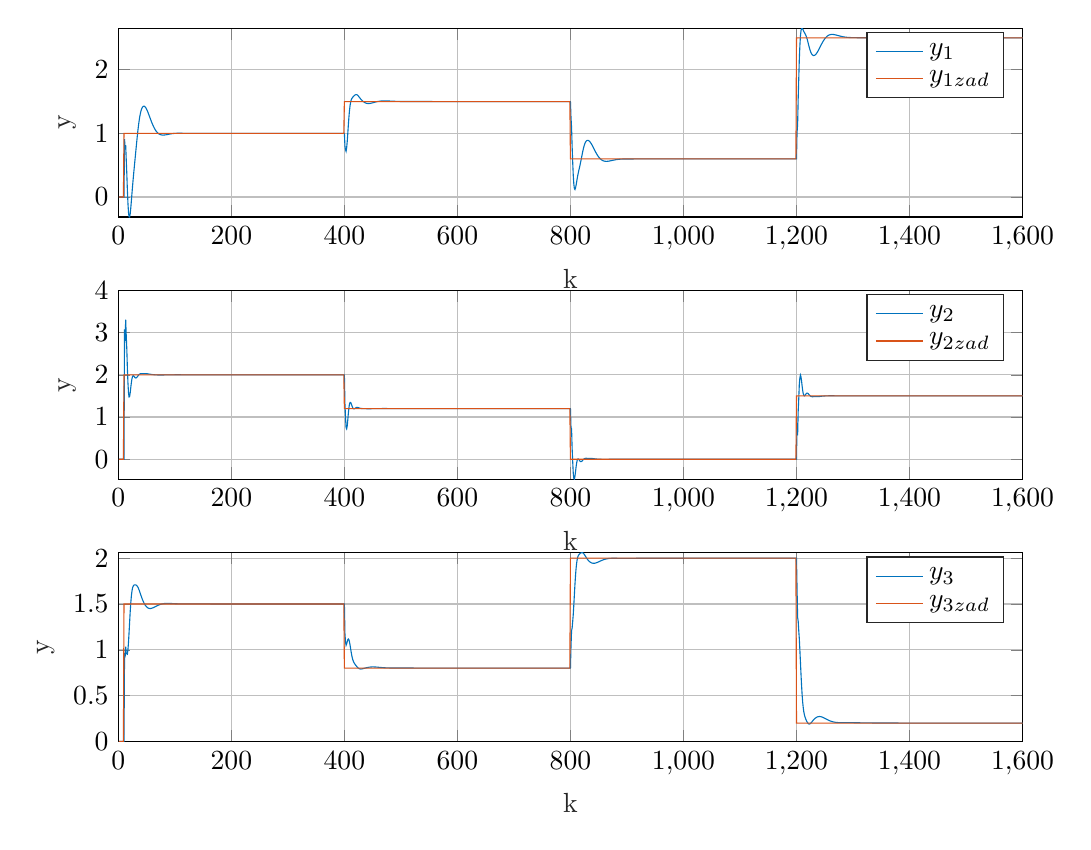
\begin{tikzpicture}

\begin{axis}[%
width=4.521in,
height=0.944in,
at={(0.758in,3.103in)},
scale only axis,
xmin=0,
xmax=1600,
xlabel style={font=\color{white!15!black}},
xlabel={k},
ymin=-0.3153,
ymax=2.6528,
ylabel style={font=\color{white!15!black}},
ylabel={y},
axis background/.style={fill=white},
xmajorgrids,
ymajorgrids,
legend style={legend cell align=left, align=left, draw=white!15!black}
]
\addplot [color=mycolor1]
  table[row sep=crcr]{%
1	0\\
2	0\\
3	0\\
4	0\\
5	0\\
6	0\\
7	0\\
8	0\\
9	0\\
10	0\\
11	0.91262\\
12	0.75093\\
13	0.81473\\
14	0.58421\\
15	0.36668\\
16	0.10856\\
17	-0.096623\\
18	-0.24329\\
19	-0.31292\\
20	-0.3153\\
21	-0.26329\\
22	-0.17584\\
23	-0.06956\\
24	0.042359\\
25	0.15199\\
26	0.2559\\
27	0.35411\\
28	0.44836\\
29	0.54082\\
30	0.63305\\
31	0.7255\\
32	0.81751\\
33	0.90755\\
34	0.99368\\
35	1.0739\\
36	1.1467\\
37	1.2109\\
38	1.2661\\
39	1.3121\\
40	1.3494\\
41	1.3786\\
42	1.4003\\
43	1.4153\\
44	1.4242\\
45	1.4276\\
46	1.426\\
47	1.4199\\
48	1.4098\\
49	1.3963\\
50	1.3797\\
51	1.3606\\
52	1.3396\\
53	1.3171\\
54	1.2936\\
55	1.2696\\
56	1.2454\\
57	1.2213\\
58	1.1978\\
59	1.1749\\
60	1.153\\
61	1.1321\\
62	1.1124\\
63	1.094\\
64	1.077\\
65	1.0614\\
66	1.0472\\
67	1.0344\\
68	1.0231\\
69	1.0131\\
70	1.0044\\
71	0.99702\\
72	0.99079\\
73	0.98566\\
74	0.98154\\
75	0.97835\\
76	0.976\\
77	0.9744\\
78	0.97345\\
79	0.97309\\
80	0.97322\\
81	0.97377\\
82	0.97467\\
83	0.97586\\
84	0.97725\\
85	0.97882\\
86	0.98049\\
87	0.98223\\
88	0.984\\
89	0.98576\\
90	0.98749\\
91	0.98916\\
92	0.99075\\
93	0.99224\\
94	0.99363\\
95	0.9949\\
96	0.99606\\
97	0.99709\\
98	0.99801\\
99	0.9988\\
100	0.99948\\
101	1\\
102	1.0005\\
103	1.0009\\
104	1.0012\\
105	1.0014\\
106	1.0015\\
107	1.0015\\
108	1.0015\\
109	1.0015\\
110	1.0014\\
111	1.0013\\
112	1.0012\\
113	1.001\\
114	1.0008\\
115	1.0006\\
116	1.0005\\
117	1.0003\\
118	1.0001\\
119	0.99992\\
120	0.99976\\
121	0.9996\\
122	0.99946\\
123	0.99934\\
124	0.99922\\
125	0.99912\\
126	0.99904\\
127	0.99897\\
128	0.99892\\
129	0.99888\\
130	0.99885\\
131	0.99883\\
132	0.99883\\
133	0.99883\\
134	0.99884\\
135	0.99887\\
136	0.9989\\
137	0.99893\\
138	0.99897\\
139	0.99901\\
140	0.99906\\
141	0.99911\\
142	0.99916\\
143	0.99921\\
144	0.99926\\
145	0.99931\\
146	0.99936\\
147	0.99941\\
148	0.99946\\
149	0.9995\\
150	0.99954\\
151	0.99959\\
152	0.99962\\
153	0.99966\\
154	0.99969\\
155	0.99972\\
156	0.99975\\
157	0.99977\\
158	0.99979\\
159	0.99982\\
160	0.99983\\
161	0.99985\\
162	0.99986\\
163	0.99988\\
164	0.99989\\
165	0.9999\\
166	0.9999\\
167	0.99991\\
168	0.99992\\
169	0.99992\\
170	0.99993\\
171	0.99993\\
172	0.99993\\
173	0.99993\\
174	0.99994\\
175	0.99994\\
176	0.99994\\
177	0.99994\\
178	0.99994\\
179	0.99994\\
180	0.99995\\
181	0.99995\\
182	0.99995\\
183	0.99995\\
184	0.99995\\
185	0.99995\\
186	0.99995\\
187	0.99995\\
188	0.99996\\
189	0.99996\\
190	0.99996\\
191	0.99996\\
192	0.99996\\
193	0.99996\\
194	0.99996\\
195	0.99997\\
196	0.99997\\
197	0.99997\\
198	0.99997\\
199	0.99997\\
200	0.99997\\
201	0.99998\\
202	0.99998\\
203	0.99998\\
204	0.99998\\
205	0.99998\\
206	0.99998\\
207	0.99998\\
208	0.99998\\
209	0.99999\\
210	0.99999\\
211	0.99999\\
212	0.99999\\
213	0.99999\\
214	0.99999\\
215	0.99999\\
216	0.99999\\
217	0.99999\\
218	0.99999\\
219	0.99999\\
220	0.99999\\
221	0.99999\\
222	0.99999\\
223	0.99999\\
224	0.99999\\
225	0.99999\\
226	1\\
227	1\\
228	1\\
229	1\\
230	1\\
231	1\\
232	1\\
233	1\\
234	1\\
235	1\\
236	1\\
237	1\\
238	1\\
239	1\\
240	1\\
241	1\\
242	1\\
243	1\\
244	1\\
245	1\\
246	1\\
247	1\\
248	1\\
249	1\\
250	1\\
251	1\\
252	1\\
253	1\\
254	1\\
255	1\\
256	1\\
257	1\\
258	1\\
259	1\\
260	1\\
261	1\\
262	1\\
263	1\\
264	1\\
265	1\\
266	1\\
267	1\\
268	1\\
269	1\\
270	1\\
271	1\\
272	1\\
273	1\\
274	1\\
275	1\\
276	1\\
277	1\\
278	1\\
279	1\\
280	1\\
281	1\\
282	1\\
283	1\\
284	1\\
285	1\\
286	1\\
287	1\\
288	1\\
289	1\\
290	1\\
291	1\\
292	1\\
293	1\\
294	1\\
295	1\\
296	1\\
297	1\\
298	1\\
299	1\\
300	1\\
301	1\\
302	1\\
303	1\\
304	1\\
305	1\\
306	1\\
307	1\\
308	1\\
309	1\\
310	1\\
311	1\\
312	1\\
313	1\\
314	1\\
315	1\\
316	1\\
317	1\\
318	1\\
319	1\\
320	1\\
321	1\\
322	1\\
323	1\\
324	1\\
325	1\\
326	1\\
327	1\\
328	1\\
329	1\\
330	1\\
331	1\\
332	1\\
333	1\\
334	1\\
335	1\\
336	1\\
337	1\\
338	1\\
339	1\\
340	1\\
341	1\\
342	1\\
343	1\\
344	1\\
345	1\\
346	1\\
347	1\\
348	1\\
349	1\\
350	1\\
351	1\\
352	1\\
353	1\\
354	1\\
355	1\\
356	1\\
357	1\\
358	1\\
359	1\\
360	1\\
361	1\\
362	1\\
363	1\\
364	1\\
365	1\\
366	1\\
367	1\\
368	1\\
369	1\\
370	1\\
371	1\\
372	1\\
373	1\\
374	1\\
375	1\\
376	1\\
377	1\\
378	1\\
379	1\\
380	1\\
381	1\\
382	1\\
383	1\\
384	1\\
385	1\\
386	1\\
387	1\\
388	1\\
389	1\\
390	1\\
391	1\\
392	1\\
393	1\\
394	1\\
395	1\\
396	1\\
397	1\\
398	1\\
399	1\\
400	1\\
401	0.79673\\
402	0.74089\\
403	0.71712\\
404	0.77179\\
405	0.86812\\
406	0.99543\\
407	1.1285\\
408	1.2522\\
409	1.355\\
410	1.4331\\
411	1.4876\\
412	1.5229\\
413	1.5449\\
414	1.5591\\
415	1.5698\\
416	1.5793\\
417	1.5884\\
418	1.597\\
419	1.604\\
420	1.6085\\
421	1.6098\\
422	1.6076\\
423	1.6021\\
424	1.5939\\
425	1.5838\\
426	1.5725\\
427	1.5609\\
428	1.5495\\
429	1.5385\\
430	1.5284\\
431	1.5191\\
432	1.5106\\
433	1.503\\
434	1.4961\\
435	1.49\\
436	1.4847\\
437	1.4802\\
438	1.4764\\
439	1.4735\\
440	1.4713\\
441	1.4699\\
442	1.4692\\
443	1.4691\\
444	1.4696\\
445	1.4706\\
446	1.4719\\
447	1.4737\\
448	1.4756\\
449	1.4778\\
450	1.4801\\
451	1.4825\\
452	1.485\\
453	1.4875\\
454	1.4899\\
455	1.4923\\
456	1.4946\\
457	1.4967\\
458	1.4988\\
459	1.5007\\
460	1.5024\\
461	1.504\\
462	1.5053\\
463	1.5066\\
464	1.5076\\
465	1.5085\\
466	1.5092\\
467	1.5098\\
468	1.5102\\
469	1.5105\\
470	1.5107\\
471	1.5107\\
472	1.5107\\
473	1.5106\\
474	1.5104\\
475	1.5101\\
476	1.5098\\
477	1.5094\\
478	1.509\\
479	1.5086\\
480	1.5081\\
481	1.5077\\
482	1.5072\\
483	1.5067\\
484	1.5063\\
485	1.5058\\
486	1.5054\\
487	1.5049\\
488	1.5045\\
489	1.5042\\
490	1.5038\\
491	1.5035\\
492	1.5031\\
493	1.5029\\
494	1.5026\\
495	1.5023\\
496	1.5021\\
497	1.5019\\
498	1.5018\\
499	1.5016\\
500	1.5015\\
501	1.5013\\
502	1.5012\\
503	1.5011\\
504	1.501\\
505	1.501\\
506	1.5009\\
507	1.5009\\
508	1.5008\\
509	1.5008\\
510	1.5007\\
511	1.5007\\
512	1.5007\\
513	1.5007\\
514	1.5006\\
515	1.5006\\
516	1.5006\\
517	1.5006\\
518	1.5006\\
519	1.5006\\
520	1.5005\\
521	1.5005\\
522	1.5005\\
523	1.5005\\
524	1.5005\\
525	1.5005\\
526	1.5004\\
527	1.5004\\
528	1.5004\\
529	1.5004\\
530	1.5004\\
531	1.5004\\
532	1.5003\\
533	1.5003\\
534	1.5003\\
535	1.5003\\
536	1.5003\\
537	1.5003\\
538	1.5002\\
539	1.5002\\
540	1.5002\\
541	1.5002\\
542	1.5002\\
543	1.5002\\
544	1.5001\\
545	1.5001\\
546	1.5001\\
547	1.5001\\
548	1.5001\\
549	1.5001\\
550	1.5001\\
551	1.5001\\
552	1.5001\\
553	1.5001\\
554	1.5001\\
555	1.5001\\
556	1.5\\
557	1.5\\
558	1.5\\
559	1.5\\
560	1.5\\
561	1.5\\
562	1.5\\
563	1.5\\
564	1.5\\
565	1.5\\
566	1.5\\
567	1.5\\
568	1.5\\
569	1.5\\
570	1.5\\
571	1.5\\
572	1.5\\
573	1.5\\
574	1.5\\
575	1.5\\
576	1.5\\
577	1.5\\
578	1.5\\
579	1.5\\
580	1.5\\
581	1.5\\
582	1.5\\
583	1.5\\
584	1.5\\
585	1.5\\
586	1.5\\
587	1.5\\
588	1.5\\
589	1.5\\
590	1.5\\
591	1.5\\
592	1.5\\
593	1.5\\
594	1.5\\
595	1.5\\
596	1.5\\
597	1.5\\
598	1.5\\
599	1.5\\
600	1.5\\
601	1.5\\
602	1.5\\
603	1.5\\
604	1.5\\
605	1.5\\
606	1.5\\
607	1.5\\
608	1.5\\
609	1.5\\
610	1.5\\
611	1.5\\
612	1.5\\
613	1.5\\
614	1.5\\
615	1.5\\
616	1.5\\
617	1.5\\
618	1.5\\
619	1.5\\
620	1.5\\
621	1.5\\
622	1.5\\
623	1.5\\
624	1.5\\
625	1.5\\
626	1.5\\
627	1.5\\
628	1.5\\
629	1.5\\
630	1.5\\
631	1.5\\
632	1.5\\
633	1.5\\
634	1.5\\
635	1.5\\
636	1.5\\
637	1.5\\
638	1.5\\
639	1.5\\
640	1.5\\
641	1.5\\
642	1.5\\
643	1.5\\
644	1.5\\
645	1.5\\
646	1.5\\
647	1.5\\
648	1.5\\
649	1.5\\
650	1.5\\
651	1.5\\
652	1.5\\
653	1.5\\
654	1.5\\
655	1.5\\
656	1.5\\
657	1.5\\
658	1.5\\
659	1.5\\
660	1.5\\
661	1.5\\
662	1.5\\
663	1.5\\
664	1.5\\
665	1.5\\
666	1.5\\
667	1.5\\
668	1.5\\
669	1.5\\
670	1.5\\
671	1.5\\
672	1.5\\
673	1.5\\
674	1.5\\
675	1.5\\
676	1.5\\
677	1.5\\
678	1.5\\
679	1.5\\
680	1.5\\
681	1.5\\
682	1.5\\
683	1.5\\
684	1.5\\
685	1.5\\
686	1.5\\
687	1.5\\
688	1.5\\
689	1.5\\
690	1.5\\
691	1.5\\
692	1.5\\
693	1.5\\
694	1.5\\
695	1.5\\
696	1.5\\
697	1.5\\
698	1.5\\
699	1.5\\
700	1.5\\
701	1.5\\
702	1.5\\
703	1.5\\
704	1.5\\
705	1.5\\
706	1.5\\
707	1.5\\
708	1.5\\
709	1.5\\
710	1.5\\
711	1.5\\
712	1.5\\
713	1.5\\
714	1.5\\
715	1.5\\
716	1.5\\
717	1.5\\
718	1.5\\
719	1.5\\
720	1.5\\
721	1.5\\
722	1.5\\
723	1.5\\
724	1.5\\
725	1.5\\
726	1.5\\
727	1.5\\
728	1.5\\
729	1.5\\
730	1.5\\
731	1.5\\
732	1.5\\
733	1.5\\
734	1.5\\
735	1.5\\
736	1.5\\
737	1.5\\
738	1.5\\
739	1.5\\
740	1.5\\
741	1.5\\
742	1.5\\
743	1.5\\
744	1.5\\
745	1.5\\
746	1.5\\
747	1.5\\
748	1.5\\
749	1.5\\
750	1.5\\
751	1.5\\
752	1.5\\
753	1.5\\
754	1.5\\
755	1.5\\
756	1.5\\
757	1.5\\
758	1.5\\
759	1.5\\
760	1.5\\
761	1.5\\
762	1.5\\
763	1.5\\
764	1.5\\
765	1.5\\
766	1.5\\
767	1.5\\
768	1.5\\
769	1.5\\
770	1.5\\
771	1.5\\
772	1.5\\
773	1.5\\
774	1.5\\
775	1.5\\
776	1.5\\
777	1.5\\
778	1.5\\
779	1.5\\
780	1.5\\
781	1.5\\
782	1.5\\
783	1.5\\
784	1.5\\
785	1.5\\
786	1.5\\
787	1.5\\
788	1.5\\
789	1.5\\
790	1.5\\
791	1.5\\
792	1.5\\
793	1.5\\
794	1.5\\
795	1.5\\
796	1.5\\
797	1.5\\
798	1.5\\
799	1.5\\
800	1.5\\
801	1.2477\\
802	1.0942\\
803	0.79188\\
804	0.55029\\
805	0.33958\\
806	0.2049\\
807	0.1328\\
808	0.11761\\
809	0.1403\\
810	0.18533\\
811	0.23867\\
812	0.29168\\
813	0.34006\\
814	0.38334\\
815	0.42319\\
816	0.46208\\
817	0.5021\\
818	0.54437\\
819	0.58887\\
820	0.63457\\
821	0.67989\\
822	0.72305\\
823	0.76247\\
824	0.79696\\
825	0.82587\\
826	0.84901\\
827	0.86656\\
828	0.87894\\
829	0.88671\\
830	0.89039\\
831	0.89049\\
832	0.88741\\
833	0.88151\\
834	0.87308\\
835	0.86242\\
836	0.84981\\
837	0.83555\\
838	0.81994\\
839	0.80333\\
840	0.78602\\
841	0.76834\\
842	0.75058\\
843	0.73298\\
844	0.71576\\
845	0.69911\\
846	0.68318\\
847	0.66808\\
848	0.65391\\
849	0.64072\\
850	0.62858\\
851	0.61749\\
852	0.60749\\
853	0.59856\\
854	0.59069\\
855	0.58385\\
856	0.57801\\
857	0.57311\\
858	0.56911\\
859	0.56594\\
860	0.56354\\
861	0.56183\\
862	0.56076\\
863	0.56025\\
864	0.56024\\
865	0.56066\\
866	0.56145\\
867	0.56255\\
868	0.5639\\
869	0.56546\\
870	0.56718\\
871	0.569\\
872	0.57091\\
873	0.57285\\
874	0.57479\\
875	0.57672\\
876	0.57861\\
877	0.58044\\
878	0.58219\\
879	0.58385\\
880	0.58542\\
881	0.58688\\
882	0.58823\\
883	0.58947\\
884	0.59061\\
885	0.59163\\
886	0.59255\\
887	0.59337\\
888	0.59409\\
889	0.59472\\
890	0.59527\\
891	0.59574\\
892	0.59614\\
893	0.59647\\
894	0.59675\\
895	0.59698\\
896	0.59716\\
897	0.59731\\
898	0.59742\\
899	0.5975\\
900	0.59756\\
901	0.59761\\
902	0.59764\\
903	0.59766\\
904	0.59768\\
905	0.59769\\
906	0.5977\\
907	0.59771\\
908	0.59772\\
909	0.59774\\
910	0.59776\\
911	0.59778\\
912	0.59781\\
913	0.59785\\
914	0.59789\\
915	0.59793\\
916	0.59799\\
917	0.59804\\
918	0.5981\\
919	0.59817\\
920	0.59824\\
921	0.59831\\
922	0.59838\\
923	0.59846\\
924	0.59853\\
925	0.59861\\
926	0.59869\\
927	0.59876\\
928	0.59884\\
929	0.59891\\
930	0.59898\\
931	0.59905\\
932	0.59911\\
933	0.59918\\
934	0.59924\\
935	0.5993\\
936	0.59935\\
937	0.5994\\
938	0.59945\\
939	0.5995\\
940	0.59954\\
941	0.59958\\
942	0.59962\\
943	0.59965\\
944	0.59968\\
945	0.59971\\
946	0.59973\\
947	0.59976\\
948	0.59978\\
949	0.5998\\
950	0.59981\\
951	0.59983\\
952	0.59984\\
953	0.59986\\
954	0.59987\\
955	0.59988\\
956	0.59989\\
957	0.59989\\
958	0.5999\\
959	0.59991\\
960	0.59991\\
961	0.59992\\
962	0.59992\\
963	0.59993\\
964	0.59993\\
965	0.59994\\
966	0.59994\\
967	0.59994\\
968	0.59995\\
969	0.59995\\
970	0.59995\\
971	0.59995\\
972	0.59996\\
973	0.59996\\
974	0.59996\\
975	0.59996\\
976	0.59997\\
977	0.59997\\
978	0.59997\\
979	0.59997\\
980	0.59997\\
981	0.59998\\
982	0.59998\\
983	0.59998\\
984	0.59998\\
985	0.59998\\
986	0.59999\\
987	0.59999\\
988	0.59999\\
989	0.59999\\
990	0.59999\\
991	0.59999\\
992	0.59999\\
993	0.59999\\
994	0.59999\\
995	0.6\\
996	0.6\\
997	0.6\\
998	0.6\\
999	0.6\\
1000	0.6\\
1001	0.6\\
1002	0.6\\
1003	0.6\\
1004	0.6\\
1005	0.6\\
1006	0.6\\
1007	0.6\\
1008	0.6\\
1009	0.6\\
1010	0.6\\
1011	0.6\\
1012	0.6\\
1013	0.6\\
1014	0.6\\
1015	0.6\\
1016	0.6\\
1017	0.6\\
1018	0.6\\
1019	0.6\\
1020	0.6\\
1021	0.6\\
1022	0.6\\
1023	0.6\\
1024	0.6\\
1025	0.6\\
1026	0.6\\
1027	0.6\\
1028	0.6\\
1029	0.6\\
1030	0.6\\
1031	0.6\\
1032	0.6\\
1033	0.6\\
1034	0.6\\
1035	0.6\\
1036	0.6\\
1037	0.6\\
1038	0.6\\
1039	0.6\\
1040	0.6\\
1041	0.6\\
1042	0.6\\
1043	0.6\\
1044	0.6\\
1045	0.6\\
1046	0.6\\
1047	0.6\\
1048	0.6\\
1049	0.6\\
1050	0.6\\
1051	0.6\\
1052	0.6\\
1053	0.6\\
1054	0.6\\
1055	0.6\\
1056	0.6\\
1057	0.6\\
1058	0.6\\
1059	0.6\\
1060	0.6\\
1061	0.6\\
1062	0.6\\
1063	0.6\\
1064	0.6\\
1065	0.6\\
1066	0.6\\
1067	0.6\\
1068	0.6\\
1069	0.6\\
1070	0.6\\
1071	0.6\\
1072	0.6\\
1073	0.6\\
1074	0.6\\
1075	0.6\\
1076	0.6\\
1077	0.6\\
1078	0.6\\
1079	0.6\\
1080	0.6\\
1081	0.6\\
1082	0.6\\
1083	0.6\\
1084	0.6\\
1085	0.6\\
1086	0.6\\
1087	0.6\\
1088	0.6\\
1089	0.6\\
1090	0.6\\
1091	0.6\\
1092	0.6\\
1093	0.6\\
1094	0.6\\
1095	0.6\\
1096	0.6\\
1097	0.6\\
1098	0.6\\
1099	0.6\\
1100	0.6\\
1101	0.6\\
1102	0.6\\
1103	0.6\\
1104	0.6\\
1105	0.6\\
1106	0.6\\
1107	0.6\\
1108	0.6\\
1109	0.6\\
1110	0.6\\
1111	0.6\\
1112	0.6\\
1113	0.6\\
1114	0.6\\
1115	0.6\\
1116	0.6\\
1117	0.6\\
1118	0.6\\
1119	0.6\\
1120	0.6\\
1121	0.6\\
1122	0.6\\
1123	0.6\\
1124	0.6\\
1125	0.6\\
1126	0.6\\
1127	0.6\\
1128	0.6\\
1129	0.6\\
1130	0.6\\
1131	0.6\\
1132	0.6\\
1133	0.6\\
1134	0.6\\
1135	0.6\\
1136	0.6\\
1137	0.6\\
1138	0.6\\
1139	0.6\\
1140	0.6\\
1141	0.6\\
1142	0.6\\
1143	0.6\\
1144	0.6\\
1145	0.6\\
1146	0.6\\
1147	0.6\\
1148	0.6\\
1149	0.6\\
1150	0.6\\
1151	0.6\\
1152	0.6\\
1153	0.6\\
1154	0.6\\
1155	0.6\\
1156	0.6\\
1157	0.6\\
1158	0.6\\
1159	0.6\\
1160	0.6\\
1161	0.6\\
1162	0.6\\
1163	0.6\\
1164	0.6\\
1165	0.6\\
1166	0.6\\
1167	0.6\\
1168	0.6\\
1169	0.6\\
1170	0.6\\
1171	0.6\\
1172	0.6\\
1173	0.6\\
1174	0.6\\
1175	0.6\\
1176	0.6\\
1177	0.6\\
1178	0.6\\
1179	0.6\\
1180	0.6\\
1181	0.6\\
1182	0.6\\
1183	0.6\\
1184	0.6\\
1185	0.6\\
1186	0.6\\
1187	0.6\\
1188	0.6\\
1189	0.6\\
1190	0.6\\
1191	0.6\\
1192	0.6\\
1193	0.6\\
1194	0.6\\
1195	0.6\\
1196	0.6\\
1197	0.6\\
1198	0.6\\
1199	0.6\\
1200	0.6\\
1201	1.0186\\
1202	1.1368\\
1203	1.5434\\
1204	1.8537\\
1205	2.1601\\
1206	2.3783\\
1207	2.5307\\
1208	2.6142\\
1209	2.6498\\
1210	2.6528\\
1211	2.6395\\
1212	2.6205\\
1213	2.6017\\
1214	2.585\\
1215	2.5692\\
1216	2.5524\\
1217	2.5321\\
1218	2.5073\\
1219	2.4777\\
1220	2.4443\\
1221	2.4089\\
1222	2.3734\\
1223	2.3397\\
1224	2.3093\\
1225	2.2834\\
1226	2.2623\\
1227	2.2462\\
1228	2.2348\\
1229	2.2276\\
1230	2.2242\\
1231	2.2243\\
1232	2.2273\\
1233	2.233\\
1234	2.2411\\
1235	2.2514\\
1236	2.2636\\
1237	2.2776\\
1238	2.2929\\
1239	2.3093\\
1240	2.3265\\
1241	2.3441\\
1242	2.3619\\
1243	2.3796\\
1244	2.397\\
1245	2.4139\\
1246	2.4301\\
1247	2.4455\\
1248	2.46\\
1249	2.4735\\
1250	2.486\\
1251	2.4974\\
1252	2.5076\\
1253	2.5168\\
1254	2.5249\\
1255	2.532\\
1256	2.5379\\
1257	2.5429\\
1258	2.547\\
1259	2.5502\\
1260	2.5525\\
1261	2.5541\\
1262	2.5551\\
1263	2.5554\\
1264	2.5552\\
1265	2.5545\\
1266	2.5534\\
1267	2.5519\\
1268	2.5502\\
1269	2.5482\\
1270	2.5461\\
1271	2.5438\\
1272	2.5414\\
1273	2.539\\
1274	2.5366\\
1275	2.5342\\
1276	2.5318\\
1277	2.5295\\
1278	2.5273\\
1279	2.5251\\
1280	2.5231\\
1281	2.5212\\
1282	2.5194\\
1283	2.5177\\
1284	2.5162\\
1285	2.5148\\
1286	2.5135\\
1287	2.5123\\
1288	2.5112\\
1289	2.5103\\
1290	2.5094\\
1291	2.5086\\
1292	2.508\\
1293	2.5074\\
1294	2.5068\\
1295	2.5064\\
1296	2.506\\
1297	2.5057\\
1298	2.5054\\
1299	2.5051\\
1300	2.5049\\
1301	2.5047\\
1302	2.5045\\
1303	2.5044\\
1304	2.5042\\
1305	2.5041\\
1306	2.504\\
1307	2.5039\\
1308	2.5038\\
1309	2.5037\\
1310	2.5036\\
1311	2.5035\\
1312	2.5034\\
1313	2.5033\\
1314	2.5032\\
1315	2.5031\\
1316	2.503\\
1317	2.5029\\
1318	2.5027\\
1319	2.5026\\
1320	2.5025\\
1321	2.5024\\
1322	2.5023\\
1323	2.5022\\
1324	2.5021\\
1325	2.502\\
1326	2.5019\\
1327	2.5017\\
1328	2.5016\\
1329	2.5015\\
1330	2.5014\\
1331	2.5013\\
1332	2.5013\\
1333	2.5012\\
1334	2.5011\\
1335	2.501\\
1336	2.5009\\
1337	2.5009\\
1338	2.5008\\
1339	2.5007\\
1340	2.5007\\
1341	2.5006\\
1342	2.5006\\
1343	2.5005\\
1344	2.5005\\
1345	2.5004\\
1346	2.5004\\
1347	2.5004\\
1348	2.5003\\
1349	2.5003\\
1350	2.5003\\
1351	2.5003\\
1352	2.5002\\
1353	2.5002\\
1354	2.5002\\
1355	2.5002\\
1356	2.5002\\
1357	2.5002\\
1358	2.5001\\
1359	2.5001\\
1360	2.5001\\
1361	2.5001\\
1362	2.5001\\
1363	2.5001\\
1364	2.5001\\
1365	2.5001\\
1366	2.5001\\
1367	2.5001\\
1368	2.5001\\
1369	2.5001\\
1370	2.5001\\
1371	2.5001\\
1372	2.5001\\
1373	2.5\\
1374	2.5\\
1375	2.5\\
1376	2.5\\
1377	2.5\\
1378	2.5\\
1379	2.5\\
1380	2.5\\
1381	2.5\\
1382	2.5\\
1383	2.5\\
1384	2.5\\
1385	2.5\\
1386	2.5\\
1387	2.5\\
1388	2.5\\
1389	2.5\\
1390	2.5\\
1391	2.5\\
1392	2.5\\
1393	2.5\\
1394	2.5\\
1395	2.5\\
1396	2.5\\
1397	2.5\\
1398	2.5\\
1399	2.5\\
1400	2.5\\
1401	2.5\\
1402	2.5\\
1403	2.5\\
1404	2.5\\
1405	2.5\\
1406	2.5\\
1407	2.5\\
1408	2.5\\
1409	2.5\\
1410	2.5\\
1411	2.5\\
1412	2.5\\
1413	2.5\\
1414	2.5\\
1415	2.5\\
1416	2.5\\
1417	2.5\\
1418	2.5\\
1419	2.5\\
1420	2.5\\
1421	2.5\\
1422	2.5\\
1423	2.5\\
1424	2.5\\
1425	2.5\\
1426	2.5\\
1427	2.5\\
1428	2.5\\
1429	2.5\\
1430	2.5\\
1431	2.5\\
1432	2.5\\
1433	2.5\\
1434	2.5\\
1435	2.5\\
1436	2.5\\
1437	2.5\\
1438	2.5\\
1439	2.5\\
1440	2.5\\
1441	2.5\\
1442	2.5\\
1443	2.5\\
1444	2.5\\
1445	2.5\\
1446	2.5\\
1447	2.5\\
1448	2.5\\
1449	2.5\\
1450	2.5\\
1451	2.5\\
1452	2.5\\
1453	2.5\\
1454	2.5\\
1455	2.5\\
1456	2.5\\
1457	2.5\\
1458	2.5\\
1459	2.5\\
1460	2.5\\
1461	2.5\\
1462	2.5\\
1463	2.5\\
1464	2.5\\
1465	2.5\\
1466	2.5\\
1467	2.5\\
1468	2.5\\
1469	2.5\\
1470	2.5\\
1471	2.5\\
1472	2.5\\
1473	2.5\\
1474	2.5\\
1475	2.5\\
1476	2.5\\
1477	2.5\\
1478	2.5\\
1479	2.5\\
1480	2.5\\
1481	2.5\\
1482	2.5\\
1483	2.5\\
1484	2.5\\
1485	2.5\\
1486	2.5\\
1487	2.5\\
1488	2.5\\
1489	2.5\\
1490	2.5\\
1491	2.5\\
1492	2.5\\
1493	2.5\\
1494	2.5\\
1495	2.5\\
1496	2.5\\
1497	2.5\\
1498	2.5\\
1499	2.5\\
1500	2.5\\
1501	2.5\\
1502	2.5\\
1503	2.5\\
1504	2.5\\
1505	2.5\\
1506	2.5\\
1507	2.5\\
1508	2.5\\
1509	2.5\\
1510	2.5\\
1511	2.5\\
1512	2.5\\
1513	2.5\\
1514	2.5\\
1515	2.5\\
1516	2.5\\
1517	2.5\\
1518	2.5\\
1519	2.5\\
1520	2.5\\
1521	2.5\\
1522	2.5\\
1523	2.5\\
1524	2.5\\
1525	2.5\\
1526	2.5\\
1527	2.5\\
1528	2.5\\
1529	2.5\\
1530	2.5\\
1531	2.5\\
1532	2.5\\
1533	2.5\\
1534	2.5\\
1535	2.5\\
1536	2.5\\
1537	2.5\\
1538	2.5\\
1539	2.5\\
1540	2.5\\
1541	2.5\\
1542	2.5\\
1543	2.5\\
1544	2.5\\
1545	2.5\\
1546	2.5\\
1547	2.5\\
1548	2.5\\
1549	2.5\\
1550	2.5\\
1551	2.5\\
1552	2.5\\
1553	2.5\\
1554	2.5\\
1555	2.5\\
1556	2.5\\
1557	2.5\\
1558	2.5\\
1559	2.5\\
1560	2.5\\
1561	2.5\\
1562	2.5\\
1563	2.5\\
1564	2.5\\
1565	2.5\\
1566	2.5\\
1567	2.5\\
1568	2.5\\
1569	2.5\\
1570	2.5\\
1571	2.5\\
1572	2.5\\
1573	2.5\\
1574	2.5\\
1575	2.5\\
1576	2.5\\
1577	2.5\\
1578	2.5\\
1579	2.5\\
1580	2.5\\
1581	2.5\\
1582	2.5\\
1583	2.5\\
1584	2.5\\
1585	2.5\\
1586	2.5\\
1587	2.5\\
1588	2.5\\
1589	2.5\\
1590	2.5\\
1591	2.5\\
1592	2.5\\
1593	2.5\\
1594	2.5\\
1595	2.5\\
1596	2.5\\
1597	2.5\\
1598	2.5\\
1599	2.5\\
1600	2.5\\
};
\addlegendentry{$\text{y}_\text{1}$}

\addplot [color=mycolor2]
  table[row sep=crcr]{%
1	0\\
2	0\\
3	0\\
4	0\\
5	0\\
6	0\\
7	0\\
8	0\\
9	0\\
10	1\\
11	1\\
12	1\\
13	1\\
14	1\\
15	1\\
16	1\\
17	1\\
18	1\\
19	1\\
20	1\\
21	1\\
22	1\\
23	1\\
24	1\\
25	1\\
26	1\\
27	1\\
28	1\\
29	1\\
30	1\\
31	1\\
32	1\\
33	1\\
34	1\\
35	1\\
36	1\\
37	1\\
38	1\\
39	1\\
40	1\\
41	1\\
42	1\\
43	1\\
44	1\\
45	1\\
46	1\\
47	1\\
48	1\\
49	1\\
50	1\\
51	1\\
52	1\\
53	1\\
54	1\\
55	1\\
56	1\\
57	1\\
58	1\\
59	1\\
60	1\\
61	1\\
62	1\\
63	1\\
64	1\\
65	1\\
66	1\\
67	1\\
68	1\\
69	1\\
70	1\\
71	1\\
72	1\\
73	1\\
74	1\\
75	1\\
76	1\\
77	1\\
78	1\\
79	1\\
80	1\\
81	1\\
82	1\\
83	1\\
84	1\\
85	1\\
86	1\\
87	1\\
88	1\\
89	1\\
90	1\\
91	1\\
92	1\\
93	1\\
94	1\\
95	1\\
96	1\\
97	1\\
98	1\\
99	1\\
100	1\\
101	1\\
102	1\\
103	1\\
104	1\\
105	1\\
106	1\\
107	1\\
108	1\\
109	1\\
110	1\\
111	1\\
112	1\\
113	1\\
114	1\\
115	1\\
116	1\\
117	1\\
118	1\\
119	1\\
120	1\\
121	1\\
122	1\\
123	1\\
124	1\\
125	1\\
126	1\\
127	1\\
128	1\\
129	1\\
130	1\\
131	1\\
132	1\\
133	1\\
134	1\\
135	1\\
136	1\\
137	1\\
138	1\\
139	1\\
140	1\\
141	1\\
142	1\\
143	1\\
144	1\\
145	1\\
146	1\\
147	1\\
148	1\\
149	1\\
150	1\\
151	1\\
152	1\\
153	1\\
154	1\\
155	1\\
156	1\\
157	1\\
158	1\\
159	1\\
160	1\\
161	1\\
162	1\\
163	1\\
164	1\\
165	1\\
166	1\\
167	1\\
168	1\\
169	1\\
170	1\\
171	1\\
172	1\\
173	1\\
174	1\\
175	1\\
176	1\\
177	1\\
178	1\\
179	1\\
180	1\\
181	1\\
182	1\\
183	1\\
184	1\\
185	1\\
186	1\\
187	1\\
188	1\\
189	1\\
190	1\\
191	1\\
192	1\\
193	1\\
194	1\\
195	1\\
196	1\\
197	1\\
198	1\\
199	1\\
200	1\\
201	1\\
202	1\\
203	1\\
204	1\\
205	1\\
206	1\\
207	1\\
208	1\\
209	1\\
210	1\\
211	1\\
212	1\\
213	1\\
214	1\\
215	1\\
216	1\\
217	1\\
218	1\\
219	1\\
220	1\\
221	1\\
222	1\\
223	1\\
224	1\\
225	1\\
226	1\\
227	1\\
228	1\\
229	1\\
230	1\\
231	1\\
232	1\\
233	1\\
234	1\\
235	1\\
236	1\\
237	1\\
238	1\\
239	1\\
240	1\\
241	1\\
242	1\\
243	1\\
244	1\\
245	1\\
246	1\\
247	1\\
248	1\\
249	1\\
250	1\\
251	1\\
252	1\\
253	1\\
254	1\\
255	1\\
256	1\\
257	1\\
258	1\\
259	1\\
260	1\\
261	1\\
262	1\\
263	1\\
264	1\\
265	1\\
266	1\\
267	1\\
268	1\\
269	1\\
270	1\\
271	1\\
272	1\\
273	1\\
274	1\\
275	1\\
276	1\\
277	1\\
278	1\\
279	1\\
280	1\\
281	1\\
282	1\\
283	1\\
284	1\\
285	1\\
286	1\\
287	1\\
288	1\\
289	1\\
290	1\\
291	1\\
292	1\\
293	1\\
294	1\\
295	1\\
296	1\\
297	1\\
298	1\\
299	1\\
300	1\\
301	1\\
302	1\\
303	1\\
304	1\\
305	1\\
306	1\\
307	1\\
308	1\\
309	1\\
310	1\\
311	1\\
312	1\\
313	1\\
314	1\\
315	1\\
316	1\\
317	1\\
318	1\\
319	1\\
320	1\\
321	1\\
322	1\\
323	1\\
324	1\\
325	1\\
326	1\\
327	1\\
328	1\\
329	1\\
330	1\\
331	1\\
332	1\\
333	1\\
334	1\\
335	1\\
336	1\\
337	1\\
338	1\\
339	1\\
340	1\\
341	1\\
342	1\\
343	1\\
344	1\\
345	1\\
346	1\\
347	1\\
348	1\\
349	1\\
350	1\\
351	1\\
352	1\\
353	1\\
354	1\\
355	1\\
356	1\\
357	1\\
358	1\\
359	1\\
360	1\\
361	1\\
362	1\\
363	1\\
364	1\\
365	1\\
366	1\\
367	1\\
368	1\\
369	1\\
370	1\\
371	1\\
372	1\\
373	1\\
374	1\\
375	1\\
376	1\\
377	1\\
378	1\\
379	1\\
380	1\\
381	1\\
382	1\\
383	1\\
384	1\\
385	1\\
386	1\\
387	1\\
388	1\\
389	1\\
390	1\\
391	1\\
392	1\\
393	1\\
394	1\\
395	1\\
396	1\\
397	1\\
398	1\\
399	1\\
400	1.5\\
401	1.5\\
402	1.5\\
403	1.5\\
404	1.5\\
405	1.5\\
406	1.5\\
407	1.5\\
408	1.5\\
409	1.5\\
410	1.5\\
411	1.5\\
412	1.5\\
413	1.5\\
414	1.5\\
415	1.5\\
416	1.5\\
417	1.5\\
418	1.5\\
419	1.5\\
420	1.5\\
421	1.5\\
422	1.5\\
423	1.5\\
424	1.5\\
425	1.5\\
426	1.5\\
427	1.5\\
428	1.5\\
429	1.5\\
430	1.5\\
431	1.5\\
432	1.5\\
433	1.5\\
434	1.5\\
435	1.5\\
436	1.5\\
437	1.5\\
438	1.5\\
439	1.5\\
440	1.5\\
441	1.5\\
442	1.5\\
443	1.5\\
444	1.5\\
445	1.5\\
446	1.5\\
447	1.5\\
448	1.5\\
449	1.5\\
450	1.5\\
451	1.5\\
452	1.5\\
453	1.5\\
454	1.5\\
455	1.5\\
456	1.5\\
457	1.5\\
458	1.5\\
459	1.5\\
460	1.5\\
461	1.5\\
462	1.5\\
463	1.5\\
464	1.5\\
465	1.5\\
466	1.5\\
467	1.5\\
468	1.5\\
469	1.5\\
470	1.5\\
471	1.5\\
472	1.5\\
473	1.5\\
474	1.5\\
475	1.5\\
476	1.5\\
477	1.5\\
478	1.5\\
479	1.5\\
480	1.5\\
481	1.5\\
482	1.5\\
483	1.5\\
484	1.5\\
485	1.5\\
486	1.5\\
487	1.5\\
488	1.5\\
489	1.5\\
490	1.5\\
491	1.5\\
492	1.5\\
493	1.5\\
494	1.5\\
495	1.5\\
496	1.5\\
497	1.5\\
498	1.5\\
499	1.5\\
500	1.5\\
501	1.5\\
502	1.5\\
503	1.5\\
504	1.5\\
505	1.5\\
506	1.5\\
507	1.5\\
508	1.5\\
509	1.5\\
510	1.5\\
511	1.5\\
512	1.5\\
513	1.5\\
514	1.5\\
515	1.5\\
516	1.5\\
517	1.5\\
518	1.5\\
519	1.5\\
520	1.5\\
521	1.5\\
522	1.5\\
523	1.5\\
524	1.5\\
525	1.5\\
526	1.5\\
527	1.5\\
528	1.5\\
529	1.5\\
530	1.5\\
531	1.5\\
532	1.5\\
533	1.5\\
534	1.5\\
535	1.5\\
536	1.5\\
537	1.5\\
538	1.5\\
539	1.5\\
540	1.5\\
541	1.5\\
542	1.5\\
543	1.5\\
544	1.5\\
545	1.5\\
546	1.5\\
547	1.5\\
548	1.5\\
549	1.5\\
550	1.5\\
551	1.5\\
552	1.5\\
553	1.5\\
554	1.5\\
555	1.5\\
556	1.5\\
557	1.5\\
558	1.5\\
559	1.5\\
560	1.5\\
561	1.5\\
562	1.5\\
563	1.5\\
564	1.5\\
565	1.5\\
566	1.5\\
567	1.5\\
568	1.5\\
569	1.5\\
570	1.5\\
571	1.5\\
572	1.5\\
573	1.5\\
574	1.5\\
575	1.5\\
576	1.5\\
577	1.5\\
578	1.5\\
579	1.5\\
580	1.5\\
581	1.5\\
582	1.5\\
583	1.5\\
584	1.5\\
585	1.5\\
586	1.5\\
587	1.5\\
588	1.5\\
589	1.5\\
590	1.5\\
591	1.5\\
592	1.5\\
593	1.5\\
594	1.5\\
595	1.5\\
596	1.5\\
597	1.5\\
598	1.5\\
599	1.5\\
600	1.5\\
601	1.5\\
602	1.5\\
603	1.5\\
604	1.5\\
605	1.5\\
606	1.5\\
607	1.5\\
608	1.5\\
609	1.5\\
610	1.5\\
611	1.5\\
612	1.5\\
613	1.5\\
614	1.5\\
615	1.5\\
616	1.5\\
617	1.5\\
618	1.5\\
619	1.5\\
620	1.5\\
621	1.5\\
622	1.5\\
623	1.5\\
624	1.5\\
625	1.5\\
626	1.5\\
627	1.5\\
628	1.5\\
629	1.5\\
630	1.5\\
631	1.5\\
632	1.5\\
633	1.5\\
634	1.5\\
635	1.5\\
636	1.5\\
637	1.5\\
638	1.5\\
639	1.5\\
640	1.5\\
641	1.5\\
642	1.5\\
643	1.5\\
644	1.5\\
645	1.5\\
646	1.5\\
647	1.5\\
648	1.5\\
649	1.5\\
650	1.5\\
651	1.5\\
652	1.5\\
653	1.5\\
654	1.5\\
655	1.5\\
656	1.5\\
657	1.5\\
658	1.5\\
659	1.5\\
660	1.5\\
661	1.5\\
662	1.5\\
663	1.5\\
664	1.5\\
665	1.5\\
666	1.5\\
667	1.5\\
668	1.5\\
669	1.5\\
670	1.5\\
671	1.5\\
672	1.5\\
673	1.5\\
674	1.5\\
675	1.5\\
676	1.5\\
677	1.5\\
678	1.5\\
679	1.5\\
680	1.5\\
681	1.5\\
682	1.5\\
683	1.5\\
684	1.5\\
685	1.5\\
686	1.5\\
687	1.5\\
688	1.5\\
689	1.5\\
690	1.5\\
691	1.5\\
692	1.5\\
693	1.5\\
694	1.5\\
695	1.5\\
696	1.5\\
697	1.5\\
698	1.5\\
699	1.5\\
700	1.5\\
701	1.5\\
702	1.5\\
703	1.5\\
704	1.5\\
705	1.5\\
706	1.5\\
707	1.5\\
708	1.5\\
709	1.5\\
710	1.5\\
711	1.5\\
712	1.5\\
713	1.5\\
714	1.5\\
715	1.5\\
716	1.5\\
717	1.5\\
718	1.5\\
719	1.5\\
720	1.5\\
721	1.5\\
722	1.5\\
723	1.5\\
724	1.5\\
725	1.5\\
726	1.5\\
727	1.5\\
728	1.5\\
729	1.5\\
730	1.5\\
731	1.5\\
732	1.5\\
733	1.5\\
734	1.5\\
735	1.5\\
736	1.5\\
737	1.5\\
738	1.5\\
739	1.5\\
740	1.5\\
741	1.5\\
742	1.5\\
743	1.5\\
744	1.5\\
745	1.5\\
746	1.5\\
747	1.5\\
748	1.5\\
749	1.5\\
750	1.5\\
751	1.5\\
752	1.5\\
753	1.5\\
754	1.5\\
755	1.5\\
756	1.5\\
757	1.5\\
758	1.5\\
759	1.5\\
760	1.5\\
761	1.5\\
762	1.5\\
763	1.5\\
764	1.5\\
765	1.5\\
766	1.5\\
767	1.5\\
768	1.5\\
769	1.5\\
770	1.5\\
771	1.5\\
772	1.5\\
773	1.5\\
774	1.5\\
775	1.5\\
776	1.5\\
777	1.5\\
778	1.5\\
779	1.5\\
780	1.5\\
781	1.5\\
782	1.5\\
783	1.5\\
784	1.5\\
785	1.5\\
786	1.5\\
787	1.5\\
788	1.5\\
789	1.5\\
790	1.5\\
791	1.5\\
792	1.5\\
793	1.5\\
794	1.5\\
795	1.5\\
796	1.5\\
797	1.5\\
798	1.5\\
799	1.5\\
800	0.6\\
801	0.6\\
802	0.6\\
803	0.6\\
804	0.6\\
805	0.6\\
806	0.6\\
807	0.6\\
808	0.6\\
809	0.6\\
810	0.6\\
811	0.6\\
812	0.6\\
813	0.6\\
814	0.6\\
815	0.6\\
816	0.6\\
817	0.6\\
818	0.6\\
819	0.6\\
820	0.6\\
821	0.6\\
822	0.6\\
823	0.6\\
824	0.6\\
825	0.6\\
826	0.6\\
827	0.6\\
828	0.6\\
829	0.6\\
830	0.6\\
831	0.6\\
832	0.6\\
833	0.6\\
834	0.6\\
835	0.6\\
836	0.6\\
837	0.6\\
838	0.6\\
839	0.6\\
840	0.6\\
841	0.6\\
842	0.6\\
843	0.6\\
844	0.6\\
845	0.6\\
846	0.6\\
847	0.6\\
848	0.6\\
849	0.6\\
850	0.6\\
851	0.6\\
852	0.6\\
853	0.6\\
854	0.6\\
855	0.6\\
856	0.6\\
857	0.6\\
858	0.6\\
859	0.6\\
860	0.6\\
861	0.6\\
862	0.6\\
863	0.6\\
864	0.6\\
865	0.6\\
866	0.6\\
867	0.6\\
868	0.6\\
869	0.6\\
870	0.6\\
871	0.6\\
872	0.6\\
873	0.6\\
874	0.6\\
875	0.6\\
876	0.6\\
877	0.6\\
878	0.6\\
879	0.6\\
880	0.6\\
881	0.6\\
882	0.6\\
883	0.6\\
884	0.6\\
885	0.6\\
886	0.6\\
887	0.6\\
888	0.6\\
889	0.6\\
890	0.6\\
891	0.6\\
892	0.6\\
893	0.6\\
894	0.6\\
895	0.6\\
896	0.6\\
897	0.6\\
898	0.6\\
899	0.6\\
900	0.6\\
901	0.6\\
902	0.6\\
903	0.6\\
904	0.6\\
905	0.6\\
906	0.6\\
907	0.6\\
908	0.6\\
909	0.6\\
910	0.6\\
911	0.6\\
912	0.6\\
913	0.6\\
914	0.6\\
915	0.6\\
916	0.6\\
917	0.6\\
918	0.6\\
919	0.6\\
920	0.6\\
921	0.6\\
922	0.6\\
923	0.6\\
924	0.6\\
925	0.6\\
926	0.6\\
927	0.6\\
928	0.6\\
929	0.6\\
930	0.6\\
931	0.6\\
932	0.6\\
933	0.6\\
934	0.6\\
935	0.6\\
936	0.6\\
937	0.6\\
938	0.6\\
939	0.6\\
940	0.6\\
941	0.6\\
942	0.6\\
943	0.6\\
944	0.6\\
945	0.6\\
946	0.6\\
947	0.6\\
948	0.6\\
949	0.6\\
950	0.6\\
951	0.6\\
952	0.6\\
953	0.6\\
954	0.6\\
955	0.6\\
956	0.6\\
957	0.6\\
958	0.6\\
959	0.6\\
960	0.6\\
961	0.6\\
962	0.6\\
963	0.6\\
964	0.6\\
965	0.6\\
966	0.6\\
967	0.6\\
968	0.6\\
969	0.6\\
970	0.6\\
971	0.6\\
972	0.6\\
973	0.6\\
974	0.6\\
975	0.6\\
976	0.6\\
977	0.6\\
978	0.6\\
979	0.6\\
980	0.6\\
981	0.6\\
982	0.6\\
983	0.6\\
984	0.6\\
985	0.6\\
986	0.6\\
987	0.6\\
988	0.6\\
989	0.6\\
990	0.6\\
991	0.6\\
992	0.6\\
993	0.6\\
994	0.6\\
995	0.6\\
996	0.6\\
997	0.6\\
998	0.6\\
999	0.6\\
1000	0.6\\
1001	0.6\\
1002	0.6\\
1003	0.6\\
1004	0.6\\
1005	0.6\\
1006	0.6\\
1007	0.6\\
1008	0.6\\
1009	0.6\\
1010	0.6\\
1011	0.6\\
1012	0.6\\
1013	0.6\\
1014	0.6\\
1015	0.6\\
1016	0.6\\
1017	0.6\\
1018	0.6\\
1019	0.6\\
1020	0.6\\
1021	0.6\\
1022	0.6\\
1023	0.6\\
1024	0.6\\
1025	0.6\\
1026	0.6\\
1027	0.6\\
1028	0.6\\
1029	0.6\\
1030	0.6\\
1031	0.6\\
1032	0.6\\
1033	0.6\\
1034	0.6\\
1035	0.6\\
1036	0.6\\
1037	0.6\\
1038	0.6\\
1039	0.6\\
1040	0.6\\
1041	0.6\\
1042	0.6\\
1043	0.6\\
1044	0.6\\
1045	0.6\\
1046	0.6\\
1047	0.6\\
1048	0.6\\
1049	0.6\\
1050	0.6\\
1051	0.6\\
1052	0.6\\
1053	0.6\\
1054	0.6\\
1055	0.6\\
1056	0.6\\
1057	0.6\\
1058	0.6\\
1059	0.6\\
1060	0.6\\
1061	0.6\\
1062	0.6\\
1063	0.6\\
1064	0.6\\
1065	0.6\\
1066	0.6\\
1067	0.6\\
1068	0.6\\
1069	0.6\\
1070	0.6\\
1071	0.6\\
1072	0.6\\
1073	0.6\\
1074	0.6\\
1075	0.6\\
1076	0.6\\
1077	0.6\\
1078	0.6\\
1079	0.6\\
1080	0.6\\
1081	0.6\\
1082	0.6\\
1083	0.6\\
1084	0.6\\
1085	0.6\\
1086	0.6\\
1087	0.6\\
1088	0.6\\
1089	0.6\\
1090	0.6\\
1091	0.6\\
1092	0.6\\
1093	0.6\\
1094	0.6\\
1095	0.6\\
1096	0.6\\
1097	0.6\\
1098	0.6\\
1099	0.6\\
1100	0.6\\
1101	0.6\\
1102	0.6\\
1103	0.6\\
1104	0.6\\
1105	0.6\\
1106	0.6\\
1107	0.6\\
1108	0.6\\
1109	0.6\\
1110	0.6\\
1111	0.6\\
1112	0.6\\
1113	0.6\\
1114	0.6\\
1115	0.6\\
1116	0.6\\
1117	0.6\\
1118	0.6\\
1119	0.6\\
1120	0.6\\
1121	0.6\\
1122	0.6\\
1123	0.6\\
1124	0.6\\
1125	0.6\\
1126	0.6\\
1127	0.6\\
1128	0.6\\
1129	0.6\\
1130	0.6\\
1131	0.6\\
1132	0.6\\
1133	0.6\\
1134	0.6\\
1135	0.6\\
1136	0.6\\
1137	0.6\\
1138	0.6\\
1139	0.6\\
1140	0.6\\
1141	0.6\\
1142	0.6\\
1143	0.6\\
1144	0.6\\
1145	0.6\\
1146	0.6\\
1147	0.6\\
1148	0.6\\
1149	0.6\\
1150	0.6\\
1151	0.6\\
1152	0.6\\
1153	0.6\\
1154	0.6\\
1155	0.6\\
1156	0.6\\
1157	0.6\\
1158	0.6\\
1159	0.6\\
1160	0.6\\
1161	0.6\\
1162	0.6\\
1163	0.6\\
1164	0.6\\
1165	0.6\\
1166	0.6\\
1167	0.6\\
1168	0.6\\
1169	0.6\\
1170	0.6\\
1171	0.6\\
1172	0.6\\
1173	0.6\\
1174	0.6\\
1175	0.6\\
1176	0.6\\
1177	0.6\\
1178	0.6\\
1179	0.6\\
1180	0.6\\
1181	0.6\\
1182	0.6\\
1183	0.6\\
1184	0.6\\
1185	0.6\\
1186	0.6\\
1187	0.6\\
1188	0.6\\
1189	0.6\\
1190	0.6\\
1191	0.6\\
1192	0.6\\
1193	0.6\\
1194	0.6\\
1195	0.6\\
1196	0.6\\
1197	0.6\\
1198	0.6\\
1199	0.6\\
1200	2.5\\
1201	2.5\\
1202	2.5\\
1203	2.5\\
1204	2.5\\
1205	2.5\\
1206	2.5\\
1207	2.5\\
1208	2.5\\
1209	2.5\\
1210	2.5\\
1211	2.5\\
1212	2.5\\
1213	2.5\\
1214	2.5\\
1215	2.5\\
1216	2.5\\
1217	2.5\\
1218	2.5\\
1219	2.5\\
1220	2.5\\
1221	2.5\\
1222	2.5\\
1223	2.5\\
1224	2.5\\
1225	2.5\\
1226	2.5\\
1227	2.5\\
1228	2.5\\
1229	2.5\\
1230	2.5\\
1231	2.5\\
1232	2.5\\
1233	2.5\\
1234	2.5\\
1235	2.5\\
1236	2.5\\
1237	2.5\\
1238	2.5\\
1239	2.5\\
1240	2.5\\
1241	2.5\\
1242	2.5\\
1243	2.5\\
1244	2.5\\
1245	2.5\\
1246	2.5\\
1247	2.5\\
1248	2.5\\
1249	2.5\\
1250	2.5\\
1251	2.5\\
1252	2.5\\
1253	2.5\\
1254	2.5\\
1255	2.5\\
1256	2.5\\
1257	2.5\\
1258	2.5\\
1259	2.5\\
1260	2.5\\
1261	2.5\\
1262	2.5\\
1263	2.5\\
1264	2.5\\
1265	2.5\\
1266	2.5\\
1267	2.5\\
1268	2.5\\
1269	2.5\\
1270	2.5\\
1271	2.5\\
1272	2.5\\
1273	2.5\\
1274	2.5\\
1275	2.5\\
1276	2.5\\
1277	2.5\\
1278	2.5\\
1279	2.5\\
1280	2.5\\
1281	2.5\\
1282	2.5\\
1283	2.5\\
1284	2.5\\
1285	2.5\\
1286	2.5\\
1287	2.5\\
1288	2.5\\
1289	2.5\\
1290	2.5\\
1291	2.5\\
1292	2.5\\
1293	2.5\\
1294	2.5\\
1295	2.5\\
1296	2.5\\
1297	2.5\\
1298	2.5\\
1299	2.5\\
1300	2.5\\
1301	2.5\\
1302	2.5\\
1303	2.5\\
1304	2.5\\
1305	2.5\\
1306	2.5\\
1307	2.5\\
1308	2.5\\
1309	2.5\\
1310	2.5\\
1311	2.5\\
1312	2.5\\
1313	2.5\\
1314	2.5\\
1315	2.5\\
1316	2.5\\
1317	2.5\\
1318	2.5\\
1319	2.5\\
1320	2.5\\
1321	2.5\\
1322	2.5\\
1323	2.5\\
1324	2.5\\
1325	2.5\\
1326	2.5\\
1327	2.5\\
1328	2.5\\
1329	2.5\\
1330	2.5\\
1331	2.5\\
1332	2.5\\
1333	2.5\\
1334	2.5\\
1335	2.5\\
1336	2.5\\
1337	2.5\\
1338	2.5\\
1339	2.5\\
1340	2.5\\
1341	2.5\\
1342	2.5\\
1343	2.5\\
1344	2.5\\
1345	2.5\\
1346	2.5\\
1347	2.5\\
1348	2.5\\
1349	2.5\\
1350	2.5\\
1351	2.5\\
1352	2.5\\
1353	2.5\\
1354	2.5\\
1355	2.5\\
1356	2.5\\
1357	2.5\\
1358	2.5\\
1359	2.5\\
1360	2.5\\
1361	2.5\\
1362	2.5\\
1363	2.5\\
1364	2.5\\
1365	2.5\\
1366	2.5\\
1367	2.5\\
1368	2.5\\
1369	2.5\\
1370	2.5\\
1371	2.5\\
1372	2.5\\
1373	2.5\\
1374	2.5\\
1375	2.5\\
1376	2.5\\
1377	2.5\\
1378	2.5\\
1379	2.5\\
1380	2.5\\
1381	2.5\\
1382	2.5\\
1383	2.5\\
1384	2.5\\
1385	2.5\\
1386	2.5\\
1387	2.5\\
1388	2.5\\
1389	2.5\\
1390	2.5\\
1391	2.5\\
1392	2.5\\
1393	2.5\\
1394	2.5\\
1395	2.5\\
1396	2.5\\
1397	2.5\\
1398	2.5\\
1399	2.5\\
1400	2.5\\
1401	2.5\\
1402	2.5\\
1403	2.5\\
1404	2.5\\
1405	2.5\\
1406	2.5\\
1407	2.5\\
1408	2.5\\
1409	2.5\\
1410	2.5\\
1411	2.5\\
1412	2.5\\
1413	2.5\\
1414	2.5\\
1415	2.5\\
1416	2.5\\
1417	2.5\\
1418	2.5\\
1419	2.5\\
1420	2.5\\
1421	2.5\\
1422	2.5\\
1423	2.5\\
1424	2.5\\
1425	2.5\\
1426	2.5\\
1427	2.5\\
1428	2.5\\
1429	2.5\\
1430	2.5\\
1431	2.5\\
1432	2.5\\
1433	2.5\\
1434	2.5\\
1435	2.5\\
1436	2.5\\
1437	2.5\\
1438	2.5\\
1439	2.5\\
1440	2.5\\
1441	2.5\\
1442	2.5\\
1443	2.5\\
1444	2.5\\
1445	2.5\\
1446	2.5\\
1447	2.5\\
1448	2.5\\
1449	2.5\\
1450	2.5\\
1451	2.5\\
1452	2.5\\
1453	2.5\\
1454	2.5\\
1455	2.5\\
1456	2.5\\
1457	2.5\\
1458	2.5\\
1459	2.5\\
1460	2.5\\
1461	2.5\\
1462	2.5\\
1463	2.5\\
1464	2.5\\
1465	2.5\\
1466	2.5\\
1467	2.5\\
1468	2.5\\
1469	2.5\\
1470	2.5\\
1471	2.5\\
1472	2.5\\
1473	2.5\\
1474	2.5\\
1475	2.5\\
1476	2.5\\
1477	2.5\\
1478	2.5\\
1479	2.5\\
1480	2.5\\
1481	2.5\\
1482	2.5\\
1483	2.5\\
1484	2.5\\
1485	2.5\\
1486	2.5\\
1487	2.5\\
1488	2.5\\
1489	2.5\\
1490	2.5\\
1491	2.5\\
1492	2.5\\
1493	2.5\\
1494	2.5\\
1495	2.5\\
1496	2.5\\
1497	2.5\\
1498	2.5\\
1499	2.5\\
1500	2.5\\
1501	2.5\\
1502	2.5\\
1503	2.5\\
1504	2.5\\
1505	2.5\\
1506	2.5\\
1507	2.5\\
1508	2.5\\
1509	2.5\\
1510	2.5\\
1511	2.5\\
1512	2.5\\
1513	2.5\\
1514	2.5\\
1515	2.5\\
1516	2.5\\
1517	2.5\\
1518	2.5\\
1519	2.5\\
1520	2.5\\
1521	2.5\\
1522	2.5\\
1523	2.5\\
1524	2.5\\
1525	2.5\\
1526	2.5\\
1527	2.5\\
1528	2.5\\
1529	2.5\\
1530	2.5\\
1531	2.5\\
1532	2.5\\
1533	2.5\\
1534	2.5\\
1535	2.5\\
1536	2.5\\
1537	2.5\\
1538	2.5\\
1539	2.5\\
1540	2.5\\
1541	2.5\\
1542	2.5\\
1543	2.5\\
1544	2.5\\
1545	2.5\\
1546	2.5\\
1547	2.5\\
1548	2.5\\
1549	2.5\\
1550	2.5\\
1551	2.5\\
1552	2.5\\
1553	2.5\\
1554	2.5\\
1555	2.5\\
1556	2.5\\
1557	2.5\\
1558	2.5\\
1559	2.5\\
1560	2.5\\
1561	2.5\\
1562	2.5\\
1563	2.5\\
1564	2.5\\
1565	2.5\\
1566	2.5\\
1567	2.5\\
1568	2.5\\
1569	2.5\\
1570	2.5\\
1571	2.5\\
1572	2.5\\
1573	2.5\\
1574	2.5\\
1575	2.5\\
1576	2.5\\
1577	2.5\\
1578	2.5\\
1579	2.5\\
1580	2.5\\
1581	2.5\\
1582	2.5\\
1583	2.5\\
1584	2.5\\
1585	2.5\\
1586	2.5\\
1587	2.5\\
1588	2.5\\
1589	2.5\\
1590	2.5\\
1591	2.5\\
1592	2.5\\
1593	2.5\\
1594	2.5\\
1595	2.5\\
1596	2.5\\
1597	2.5\\
1598	2.5\\
1599	2.5\\
1600	2.5\\
};
\addlegendentry{$\text{y}_{\text{1zad}}$}

\end{axis}

\begin{axis}[%
width=4.521in,
height=0.944in,
at={(0.758in,1.792in)},
scale only axis,
xmin=0,
xmax=1600,
xlabel style={font=\color{white!15!black}},
xlabel={k},
ymin=-0.47437,
ymax=4,
ylabel style={font=\color{white!15!black}},
ylabel={y},
axis background/.style={fill=white},
xmajorgrids,
ymajorgrids,
legend style={legend cell align=left, align=left, draw=white!15!black}
]
\addplot [color=mycolor1]
  table[row sep=crcr]{%
1	0\\
2	0\\
3	0\\
4	0\\
5	0\\
6	0\\
7	0\\
8	0\\
9	0\\
10	0\\
11	3.0764\\
12	2.8071\\
13	3.3049\\
14	2.9275\\
15	2.6131\\
16	2.1563\\
17	1.8136\\
18	1.573\\
19	1.4758\\
20	1.4873\\
21	1.5749\\
22	1.6937\\
23	1.8099\\
24	1.9004\\
25	1.956\\
26	1.9784\\
27	1.9761\\
28	1.9605\\
29	1.9424\\
30	1.9293\\
31	1.9252\\
32	1.9307\\
33	1.9438\\
34	1.9613\\
35	1.9799\\
36	1.9967\\
37	2.0102\\
38	2.0196\\
39	2.0254\\
40	2.0283\\
41	2.0292\\
42	2.0292\\
43	2.0289\\
44	2.0287\\
45	2.0287\\
46	2.0288\\
47	2.0288\\
48	2.0285\\
49	2.0279\\
50	2.0268\\
51	2.0252\\
52	2.0233\\
53	2.0211\\
54	2.0188\\
55	2.0165\\
56	2.0142\\
57	2.0121\\
58	2.0101\\
59	2.0082\\
60	2.0065\\
61	2.0049\\
62	2.0035\\
63	2.0021\\
64	2.0009\\
65	1.9999\\
66	1.9989\\
67	1.9981\\
68	1.9974\\
69	1.9969\\
70	1.9965\\
71	1.9961\\
72	1.9959\\
73	1.9958\\
74	1.9958\\
75	1.9958\\
76	1.9959\\
77	1.996\\
78	1.9962\\
79	1.9964\\
80	1.9966\\
81	1.9968\\
82	1.9971\\
83	1.9974\\
84	1.9976\\
85	1.9979\\
86	1.9982\\
87	1.9984\\
88	1.9987\\
89	1.9989\\
90	1.9991\\
91	1.9993\\
92	1.9995\\
93	1.9996\\
94	1.9998\\
95	1.9999\\
96	2\\
97	2.0001\\
98	2.0002\\
99	2.0002\\
100	2.0003\\
101	2.0003\\
102	2.0003\\
103	2.0003\\
104	2.0004\\
105	2.0004\\
106	2.0003\\
107	2.0003\\
108	2.0003\\
109	2.0003\\
110	2.0003\\
111	2.0002\\
112	2.0002\\
113	2.0002\\
114	2.0002\\
115	2.0001\\
116	2.0001\\
117	2.0001\\
118	2.0001\\
119	2\\
120	2\\
121	2\\
122	2\\
123	2\\
124	2\\
125	1.9999\\
126	1.9999\\
127	1.9999\\
128	1.9999\\
129	1.9999\\
130	1.9999\\
131	1.9999\\
132	1.9999\\
133	1.9999\\
134	1.9999\\
135	1.9999\\
136	1.9999\\
137	1.9999\\
138	1.9999\\
139	1.9999\\
140	1.9999\\
141	1.9999\\
142	1.9999\\
143	1.9999\\
144	2\\
145	2\\
146	2\\
147	2\\
148	2\\
149	2\\
150	2\\
151	2\\
152	2\\
153	2\\
154	2\\
155	2\\
156	2\\
157	2\\
158	2\\
159	2\\
160	2\\
161	2\\
162	2\\
163	2\\
164	2\\
165	2\\
166	2\\
167	2\\
168	2\\
169	2\\
170	2\\
171	2\\
172	2\\
173	2\\
174	2\\
175	2\\
176	2\\
177	2\\
178	2\\
179	2\\
180	2\\
181	2\\
182	2\\
183	2\\
184	2\\
185	2\\
186	2\\
187	2\\
188	2\\
189	2\\
190	2\\
191	2\\
192	2\\
193	2\\
194	2\\
195	2\\
196	2\\
197	2\\
198	2\\
199	2\\
200	2\\
201	2\\
202	2\\
203	2\\
204	2\\
205	2\\
206	2\\
207	2\\
208	2\\
209	2\\
210	2\\
211	2\\
212	2\\
213	2\\
214	2\\
215	2\\
216	2\\
217	2\\
218	2\\
219	2\\
220	2\\
221	2\\
222	2\\
223	2\\
224	2\\
225	2\\
226	2\\
227	2\\
228	2\\
229	2\\
230	2\\
231	2\\
232	2\\
233	2\\
234	2\\
235	2\\
236	2\\
237	2\\
238	2\\
239	2\\
240	2\\
241	2\\
242	2\\
243	2\\
244	2\\
245	2\\
246	2\\
247	2\\
248	2\\
249	2\\
250	2\\
251	2\\
252	2\\
253	2\\
254	2\\
255	2\\
256	2\\
257	2\\
258	2\\
259	2\\
260	2\\
261	2\\
262	2\\
263	2\\
264	2\\
265	2\\
266	2\\
267	2\\
268	2\\
269	2\\
270	2\\
271	2\\
272	2\\
273	2\\
274	2\\
275	2\\
276	2\\
277	2\\
278	2\\
279	2\\
280	2\\
281	2\\
282	2\\
283	2\\
284	2\\
285	2\\
286	2\\
287	2\\
288	2\\
289	2\\
290	2\\
291	2\\
292	2\\
293	2\\
294	2\\
295	2\\
296	2\\
297	2\\
298	2\\
299	2\\
300	2\\
301	2\\
302	2\\
303	2\\
304	2\\
305	2\\
306	2\\
307	2\\
308	2\\
309	2\\
310	2\\
311	2\\
312	2\\
313	2\\
314	2\\
315	2\\
316	2\\
317	2\\
318	2\\
319	2\\
320	2\\
321	2\\
322	2\\
323	2\\
324	2\\
325	2\\
326	2\\
327	2\\
328	2\\
329	2\\
330	2\\
331	2\\
332	2\\
333	2\\
334	2\\
335	2\\
336	2\\
337	2\\
338	2\\
339	2\\
340	2\\
341	2\\
342	2\\
343	2\\
344	2\\
345	2\\
346	2\\
347	2\\
348	2\\
349	2\\
350	2\\
351	2\\
352	2\\
353	2\\
354	2\\
355	2\\
356	2\\
357	2\\
358	2\\
359	2\\
360	2\\
361	2\\
362	2\\
363	2\\
364	2\\
365	2\\
366	2\\
367	2\\
368	2\\
369	2\\
370	2\\
371	2\\
372	2\\
373	2\\
374	2\\
375	2\\
376	2\\
377	2\\
378	2\\
379	2\\
380	2\\
381	2\\
382	2\\
383	2\\
384	2\\
385	2\\
386	2\\
387	2\\
388	2\\
389	2\\
390	2\\
391	2\\
392	2\\
393	2\\
394	2\\
395	2\\
396	2\\
397	2\\
398	2\\
399	2\\
400	2\\
401	1.3018\\
402	0.99049\\
403	0.74913\\
404	0.7189\\
405	0.78676\\
406	0.92964\\
407	1.0832\\
408	1.2159\\
409	1.3044\\
410	1.3452\\
411	1.3453\\
412	1.3186\\
413	1.2801\\
414	1.2424\\
415	1.2137\\
416	1.1975\\
417	1.1932\\
418	1.1976\\
419	1.2067\\
420	1.2164\\
421	1.2241\\
422	1.2283\\
423	1.2286\\
424	1.2258\\
425	1.2211\\
426	1.2158\\
427	1.2107\\
428	1.2065\\
429	1.2036\\
430	1.2018\\
431	1.2008\\
432	1.2004\\
433	1.2001\\
434	1.1999\\
435	1.1995\\
436	1.1989\\
437	1.1983\\
438	1.1976\\
439	1.197\\
440	1.1965\\
441	1.1962\\
442	1.196\\
443	1.196\\
444	1.1962\\
445	1.1963\\
446	1.1966\\
447	1.1968\\
448	1.1971\\
449	1.1974\\
450	1.1976\\
451	1.1979\\
452	1.1981\\
453	1.1983\\
454	1.1986\\
455	1.1988\\
456	1.1991\\
457	1.1993\\
458	1.1995\\
459	1.1997\\
460	1.1998\\
461	1.2\\
462	1.2001\\
463	1.2002\\
464	1.2003\\
465	1.2004\\
466	1.2004\\
467	1.2005\\
468	1.2005\\
469	1.2005\\
470	1.2005\\
471	1.2005\\
472	1.2005\\
473	1.2005\\
474	1.2005\\
475	1.2005\\
476	1.2004\\
477	1.2004\\
478	1.2004\\
479	1.2003\\
480	1.2003\\
481	1.2003\\
482	1.2002\\
483	1.2002\\
484	1.2002\\
485	1.2001\\
486	1.2001\\
487	1.2001\\
488	1.2\\
489	1.2\\
490	1.2\\
491	1.2\\
492	1.2\\
493	1.2\\
494	1.1999\\
495	1.1999\\
496	1.1999\\
497	1.1999\\
498	1.1999\\
499	1.1999\\
500	1.1999\\
501	1.1999\\
502	1.1999\\
503	1.1999\\
504	1.1999\\
505	1.1999\\
506	1.1999\\
507	1.1999\\
508	1.1999\\
509	1.1999\\
510	1.1999\\
511	1.1999\\
512	1.2\\
513	1.2\\
514	1.2\\
515	1.2\\
516	1.2\\
517	1.2\\
518	1.2\\
519	1.2\\
520	1.2\\
521	1.2\\
522	1.2\\
523	1.2\\
524	1.2\\
525	1.2\\
526	1.2\\
527	1.2\\
528	1.2\\
529	1.2\\
530	1.2\\
531	1.2\\
532	1.2\\
533	1.2\\
534	1.2\\
535	1.2\\
536	1.2\\
537	1.2\\
538	1.2\\
539	1.2\\
540	1.2\\
541	1.2\\
542	1.2\\
543	1.2\\
544	1.2\\
545	1.2\\
546	1.2\\
547	1.2\\
548	1.2\\
549	1.2\\
550	1.2\\
551	1.2\\
552	1.2\\
553	1.2\\
554	1.2\\
555	1.2\\
556	1.2\\
557	1.2\\
558	1.2\\
559	1.2\\
560	1.2\\
561	1.2\\
562	1.2\\
563	1.2\\
564	1.2\\
565	1.2\\
566	1.2\\
567	1.2\\
568	1.2\\
569	1.2\\
570	1.2\\
571	1.2\\
572	1.2\\
573	1.2\\
574	1.2\\
575	1.2\\
576	1.2\\
577	1.2\\
578	1.2\\
579	1.2\\
580	1.2\\
581	1.2\\
582	1.2\\
583	1.2\\
584	1.2\\
585	1.2\\
586	1.2\\
587	1.2\\
588	1.2\\
589	1.2\\
590	1.2\\
591	1.2\\
592	1.2\\
593	1.2\\
594	1.2\\
595	1.2\\
596	1.2\\
597	1.2\\
598	1.2\\
599	1.2\\
600	1.2\\
601	1.2\\
602	1.2\\
603	1.2\\
604	1.2\\
605	1.2\\
606	1.2\\
607	1.2\\
608	1.2\\
609	1.2\\
610	1.2\\
611	1.2\\
612	1.2\\
613	1.2\\
614	1.2\\
615	1.2\\
616	1.2\\
617	1.2\\
618	1.2\\
619	1.2\\
620	1.2\\
621	1.2\\
622	1.2\\
623	1.2\\
624	1.2\\
625	1.2\\
626	1.2\\
627	1.2\\
628	1.2\\
629	1.2\\
630	1.2\\
631	1.2\\
632	1.2\\
633	1.2\\
634	1.2\\
635	1.2\\
636	1.2\\
637	1.2\\
638	1.2\\
639	1.2\\
640	1.2\\
641	1.2\\
642	1.2\\
643	1.2\\
644	1.2\\
645	1.2\\
646	1.2\\
647	1.2\\
648	1.2\\
649	1.2\\
650	1.2\\
651	1.2\\
652	1.2\\
653	1.2\\
654	1.2\\
655	1.2\\
656	1.2\\
657	1.2\\
658	1.2\\
659	1.2\\
660	1.2\\
661	1.2\\
662	1.2\\
663	1.2\\
664	1.2\\
665	1.2\\
666	1.2\\
667	1.2\\
668	1.2\\
669	1.2\\
670	1.2\\
671	1.2\\
672	1.2\\
673	1.2\\
674	1.2\\
675	1.2\\
676	1.2\\
677	1.2\\
678	1.2\\
679	1.2\\
680	1.2\\
681	1.2\\
682	1.2\\
683	1.2\\
684	1.2\\
685	1.2\\
686	1.2\\
687	1.2\\
688	1.2\\
689	1.2\\
690	1.2\\
691	1.2\\
692	1.2\\
693	1.2\\
694	1.2\\
695	1.2\\
696	1.2\\
697	1.2\\
698	1.2\\
699	1.2\\
700	1.2\\
701	1.2\\
702	1.2\\
703	1.2\\
704	1.2\\
705	1.2\\
706	1.2\\
707	1.2\\
708	1.2\\
709	1.2\\
710	1.2\\
711	1.2\\
712	1.2\\
713	1.2\\
714	1.2\\
715	1.2\\
716	1.2\\
717	1.2\\
718	1.2\\
719	1.2\\
720	1.2\\
721	1.2\\
722	1.2\\
723	1.2\\
724	1.2\\
725	1.2\\
726	1.2\\
727	1.2\\
728	1.2\\
729	1.2\\
730	1.2\\
731	1.2\\
732	1.2\\
733	1.2\\
734	1.2\\
735	1.2\\
736	1.2\\
737	1.2\\
738	1.2\\
739	1.2\\
740	1.2\\
741	1.2\\
742	1.2\\
743	1.2\\
744	1.2\\
745	1.2\\
746	1.2\\
747	1.2\\
748	1.2\\
749	1.2\\
750	1.2\\
751	1.2\\
752	1.2\\
753	1.2\\
754	1.2\\
755	1.2\\
756	1.2\\
757	1.2\\
758	1.2\\
759	1.2\\
760	1.2\\
761	1.2\\
762	1.2\\
763	1.2\\
764	1.2\\
765	1.2\\
766	1.2\\
767	1.2\\
768	1.2\\
769	1.2\\
770	1.2\\
771	1.2\\
772	1.2\\
773	1.2\\
774	1.2\\
775	1.2\\
776	1.2\\
777	1.2\\
778	1.2\\
779	1.2\\
780	1.2\\
781	1.2\\
782	1.2\\
783	1.2\\
784	1.2\\
785	1.2\\
786	1.2\\
787	1.2\\
788	1.2\\
789	1.2\\
790	1.2\\
791	1.2\\
792	1.2\\
793	1.2\\
794	1.2\\
795	1.2\\
796	1.2\\
797	1.2\\
798	1.2\\
799	1.2\\
800	1.2\\
801	0.74699\\
802	0.72409\\
803	0.25361\\
804	-0.055169\\
805	-0.33107\\
806	-0.45401\\
807	-0.47437\\
808	-0.4066\\
809	-0.29869\\
810	-0.18348\\
811	-0.088247\\
812	-0.025205\\
813	0.0039553\\
814	0.0060049\\
815	-0.008569\\
816	-0.028942\\
817	-0.046598\\
818	-0.056465\\
819	-0.056977\\
820	-0.049295\\
821	-0.036184\\
822	-0.020884\\
823	-0.0062434\\
824	0.0057949\\
825	0.014332\\
826	0.019384\\
827	0.021589\\
828	0.021874\\
829	0.021166\\
830	0.020195\\
831	0.019411\\
832	0.018981\\
833	0.018859\\
834	0.018875\\
835	0.018823\\
836	0.018533\\
837	0.017901\\
838	0.016907\\
839	0.015594\\
840	0.014051\\
841	0.012382\\
842	0.010687\\
843	0.0090413\\
844	0.0074967\\
845	0.0060774\\
846	0.0047881\\
847	0.0036212\\
848	0.002564\\
849	0.0016044\\
850	0.00073431\\
851	-5.0132e-05\\
852	-0.00074886\\
853	-0.0013598\\
854	-0.0018808\\
855	-0.002311\\
856	-0.0026518\\
857	-0.0029073\\
858	-0.0030837\\
859	-0.0031888\\
860	-0.0032311\\
861	-0.0032195\\
862	-0.0031623\\
863	-0.0030671\\
864	-0.0029407\\
865	-0.0027893\\
866	-0.0026181\\
867	-0.0024319\\
868	-0.0022352\\
869	-0.0020321\\
870	-0.0018261\\
871	-0.0016208\\
872	-0.0014191\\
873	-0.0012237\\
874	-0.0010367\\
875	-0.00085982\\
876	-0.00069449\\
877	-0.00054165\\
878	-0.00040189\\
879	-0.00027552\\
880	-0.00016259\\
881	-6.2949e-05\\
882	2.3751e-05\\
883	9.7988e-05\\
884	0.00016036\\
885	0.00021155\\
886	0.00025233\\
887	0.00028352\\
888	0.00030596\\
889	0.00032054\\
890	0.00032812\\
891	0.00032958\\
892	0.00032576\\
893	0.00031746\\
894	0.00030547\\
895	0.00029048\\
896	0.00027318\\
897	0.00025416\\
898	0.00023397\\
899	0.00021311\\
900	0.000192\\
901	0.00017102\\
902	0.0001505\\
903	0.00013071\\
904	0.00011185\\
905	9.4117e-05\\
906	7.7629e-05\\
907	6.2485e-05\\
908	4.8742e-05\\
909	3.6428e-05\\
910	2.5544e-05\\
911	1.6067e-05\\
912	7.9547e-06\\
913	1.1484e-06\\
914	-4.4235e-06\\
915	-8.8429e-06\\
916	-1.2199e-05\\
917	-1.4585e-05\\
918	-1.61e-05\\
919	-1.6839e-05\\
920	-1.6901e-05\\
921	-1.6379e-05\\
922	-1.5366e-05\\
923	-1.3946e-05\\
924	-1.2203e-05\\
925	-1.0211e-05\\
926	-8.0394e-06\\
927	-5.7513e-06\\
928	-3.4029e-06\\
929	-1.0435e-06\\
930	1.2838e-06\\
931	3.5423e-06\\
932	5.7014e-06\\
933	7.736e-06\\
934	9.6267e-06\\
935	1.1359e-05\\
936	1.2922e-05\\
937	1.431e-05\\
938	1.552e-05\\
939	1.6554e-05\\
940	1.7414e-05\\
941	1.8106e-05\\
942	1.8637e-05\\
943	1.9017e-05\\
944	1.9256e-05\\
945	1.9366e-05\\
946	1.9356e-05\\
947	1.9241e-05\\
948	1.9032e-05\\
949	1.874e-05\\
950	1.8378e-05\\
951	1.7957e-05\\
952	1.7488e-05\\
953	1.698e-05\\
954	1.6443e-05\\
955	1.5886e-05\\
956	1.5316e-05\\
957	1.4741e-05\\
958	1.4166e-05\\
959	1.3598e-05\\
960	1.304e-05\\
961	1.2497e-05\\
962	1.1972e-05\\
963	1.1468e-05\\
964	1.0986e-05\\
965	1.0527e-05\\
966	1.0094e-05\\
967	9.6853e-06\\
968	9.3021e-06\\
969	8.9437e-06\\
970	8.6097e-06\\
971	8.2992e-06\\
972	8.0111e-06\\
973	7.7444e-06\\
974	7.4976e-06\\
975	7.2695e-06\\
976	7.0587e-06\\
977	6.8635e-06\\
978	6.6827e-06\\
979	6.5148e-06\\
980	6.3584e-06\\
981	6.2122e-06\\
982	6.075e-06\\
983	5.9456e-06\\
984	5.8229e-06\\
985	5.7059e-06\\
986	5.5937e-06\\
987	5.4855e-06\\
988	5.3807e-06\\
989	5.2785e-06\\
990	5.1784e-06\\
991	5.08e-06\\
992	4.9829e-06\\
993	4.8868e-06\\
994	4.7915e-06\\
995	4.6967e-06\\
996	4.6023e-06\\
997	4.5083e-06\\
998	4.4147e-06\\
999	4.3213e-06\\
1000	4.2283e-06\\
1001	4.1357e-06\\
1002	4.0436e-06\\
1003	3.952e-06\\
1004	3.861e-06\\
1005	3.7709e-06\\
1006	3.6816e-06\\
1007	3.5932e-06\\
1008	3.506e-06\\
1009	3.4199e-06\\
1010	3.3352e-06\\
1011	3.2518e-06\\
1012	3.1699e-06\\
1013	3.0895e-06\\
1014	3.0108e-06\\
1015	2.9337e-06\\
1016	2.8583e-06\\
1017	2.7846e-06\\
1018	2.7127e-06\\
1019	2.6426e-06\\
1020	2.5743e-06\\
1021	2.5078e-06\\
1022	2.443e-06\\
1023	2.38e-06\\
1024	2.3188e-06\\
1025	2.2593e-06\\
1026	2.2015e-06\\
1027	2.1453e-06\\
1028	2.0907e-06\\
1029	2.0377e-06\\
1030	1.9863e-06\\
1031	1.9363e-06\\
1032	1.8877e-06\\
1033	1.8405e-06\\
1034	1.7947e-06\\
1035	1.7501e-06\\
1036	1.7068e-06\\
1037	1.6647e-06\\
1038	1.6237e-06\\
1039	1.5839e-06\\
1040	1.5451e-06\\
1041	1.5073e-06\\
1042	1.4706e-06\\
1043	1.4347e-06\\
1044	1.3998e-06\\
1045	1.3658e-06\\
1046	1.3327e-06\\
1047	1.3003e-06\\
1048	1.2688e-06\\
1049	1.238e-06\\
1050	1.208e-06\\
1051	1.1787e-06\\
1052	1.1501e-06\\
1053	1.1222e-06\\
1054	1.0949e-06\\
1055	1.0683e-06\\
1056	1.0423e-06\\
1057	1.0169e-06\\
1058	9.9217e-07\\
1059	9.6799e-07\\
1060	9.4437e-07\\
1061	9.2131e-07\\
1062	8.988e-07\\
1063	8.7682e-07\\
1064	8.5537e-07\\
1065	8.3442e-07\\
1066	8.1397e-07\\
1067	7.9402e-07\\
1068	7.7454e-07\\
1069	7.5553e-07\\
1070	7.3698e-07\\
1071	7.1887e-07\\
1072	7.0121e-07\\
1073	6.8398e-07\\
1074	6.6717e-07\\
1075	6.5076e-07\\
1076	6.3476e-07\\
1077	6.1916e-07\\
1078	6.0394e-07\\
1079	5.8909e-07\\
1080	5.7461e-07\\
1081	5.6048e-07\\
1082	5.4671e-07\\
1083	5.3328e-07\\
1084	5.2018e-07\\
1085	5.074e-07\\
1086	4.9494e-07\\
1087	4.8279e-07\\
1088	4.7094e-07\\
1089	4.5939e-07\\
1090	4.4812e-07\\
1091	4.3713e-07\\
1092	4.2641e-07\\
1093	4.1596e-07\\
1094	4.0577e-07\\
1095	3.9583e-07\\
1096	3.8613e-07\\
1097	3.7667e-07\\
1098	3.6745e-07\\
1099	3.5845e-07\\
1100	3.4968e-07\\
1101	3.4112e-07\\
1102	3.3277e-07\\
1103	3.2462e-07\\
1104	3.1668e-07\\
1105	3.0893e-07\\
1106	3.0137e-07\\
1107	2.9399e-07\\
1108	2.868e-07\\
1109	2.7978e-07\\
1110	2.7294e-07\\
1111	2.6626e-07\\
1112	2.5974e-07\\
1113	2.5339e-07\\
1114	2.4719e-07\\
1115	2.4114e-07\\
1116	2.3524e-07\\
1117	2.2948e-07\\
1118	2.2386e-07\\
1119	2.1839e-07\\
1120	2.1304e-07\\
1121	2.0783e-07\\
1122	2.0274e-07\\
1123	1.9778e-07\\
1124	1.9293e-07\\
1125	1.8821e-07\\
1126	1.836e-07\\
1127	1.7911e-07\\
1128	1.7472e-07\\
1129	1.7045e-07\\
1130	1.6627e-07\\
1131	1.622e-07\\
1132	1.5823e-07\\
1133	1.5436e-07\\
1134	1.5058e-07\\
1135	1.4689e-07\\
1136	1.433e-07\\
1137	1.3979e-07\\
1138	1.3637e-07\\
1139	1.3303e-07\\
1140	1.2977e-07\\
1141	1.2659e-07\\
1142	1.2349e-07\\
1143	1.2047e-07\\
1144	1.1752e-07\\
1145	1.1465e-07\\
1146	1.1184e-07\\
1147	1.091e-07\\
1148	1.0643e-07\\
1149	1.0382e-07\\
1150	1.0128e-07\\
1151	9.8804e-08\\
1152	9.6386e-08\\
1153	9.4027e-08\\
1154	9.1725e-08\\
1155	8.948e-08\\
1156	8.729e-08\\
1157	8.5154e-08\\
1158	8.3069e-08\\
1159	8.1036e-08\\
1160	7.9053e-08\\
1161	7.7118e-08\\
1162	7.5231e-08\\
1163	7.3389e-08\\
1164	7.1593e-08\\
1165	6.9841e-08\\
1166	6.8132e-08\\
1167	6.6464e-08\\
1168	6.4838e-08\\
1169	6.3251e-08\\
1170	6.1703e-08\\
1171	6.0193e-08\\
1172	5.8719e-08\\
1173	5.7282e-08\\
1174	5.588e-08\\
1175	5.4513e-08\\
1176	5.3178e-08\\
1177	5.1877e-08\\
1178	5.0607e-08\\
1179	4.9369e-08\\
1180	4.816e-08\\
1181	4.6982e-08\\
1182	4.5832e-08\\
1183	4.471e-08\\
1184	4.3616e-08\\
1185	4.2548e-08\\
1186	4.1507e-08\\
1187	4.0491e-08\\
1188	3.95e-08\\
1189	3.8533e-08\\
1190	3.759e-08\\
1191	3.667e-08\\
1192	3.5772e-08\\
1193	3.4897e-08\\
1194	3.4043e-08\\
1195	3.321e-08\\
1196	3.2397e-08\\
1197	3.1604e-08\\
1198	3.083e-08\\
1199	3.0076e-08\\
1200	2.934e-08\\
1201	0.86219\\
1202	0.5635\\
1203	1.1345\\
1204	1.4261\\
1205	1.7712\\
1206	1.933\\
1207	1.9955\\
1208	1.9488\\
1209	1.8498\\
1210	1.7307\\
1211	1.6254\\
1212	1.5499\\
1213	1.5098\\
1214	1.5001\\
1215	1.5111\\
1216	1.5313\\
1217	1.551\\
1218	1.5639\\
1219	1.5671\\
1220	1.5613\\
1221	1.5488\\
1222	1.533\\
1223	1.517\\
1224	1.5031\\
1225	1.4927\\
1226	1.4859\\
1227	1.4823\\
1228	1.4811\\
1229	1.4811\\
1230	1.4817\\
1231	1.4822\\
1232	1.4825\\
1233	1.4823\\
1234	1.4821\\
1235	1.4818\\
1236	1.4818\\
1237	1.4821\\
1238	1.4828\\
1239	1.4839\\
1240	1.4853\\
1241	1.4869\\
1242	1.4885\\
1243	1.4902\\
1244	1.4917\\
1245	1.4932\\
1246	1.4945\\
1247	1.4957\\
1248	1.4968\\
1249	1.4979\\
1250	1.4988\\
1251	1.4996\\
1252	1.5004\\
1253	1.5011\\
1254	1.5016\\
1255	1.5021\\
1256	1.5025\\
1257	1.5028\\
1258	1.5031\\
1259	1.5032\\
1260	1.5033\\
1261	1.5033\\
1262	1.5033\\
1263	1.5032\\
1264	1.5031\\
1265	1.503\\
1266	1.5028\\
1267	1.5026\\
1268	1.5024\\
1269	1.5022\\
1270	1.502\\
1271	1.5018\\
1272	1.5016\\
1273	1.5014\\
1274	1.5012\\
1275	1.501\\
1276	1.5008\\
1277	1.5006\\
1278	1.5005\\
1279	1.5003\\
1280	1.5002\\
1281	1.5001\\
1282	1.5\\
1283	1.4999\\
1284	1.4998\\
1285	1.4998\\
1286	1.4997\\
1287	1.4997\\
1288	1.4997\\
1289	1.4996\\
1290	1.4996\\
1291	1.4996\\
1292	1.4996\\
1293	1.4996\\
1294	1.4996\\
1295	1.4996\\
1296	1.4997\\
1297	1.4997\\
1298	1.4997\\
1299	1.4997\\
1300	1.4997\\
1301	1.4998\\
1302	1.4998\\
1303	1.4998\\
1304	1.4998\\
1305	1.4998\\
1306	1.4999\\
1307	1.4999\\
1308	1.4999\\
1309	1.4999\\
1310	1.4999\\
1311	1.4999\\
1312	1.4999\\
1313	1.5\\
1314	1.5\\
1315	1.5\\
1316	1.5\\
1317	1.5\\
1318	1.5\\
1319	1.5\\
1320	1.5\\
1321	1.5\\
1322	1.5\\
1323	1.5\\
1324	1.5\\
1325	1.5\\
1326	1.5\\
1327	1.5\\
1328	1.5\\
1329	1.5\\
1330	1.5\\
1331	1.5\\
1332	1.5\\
1333	1.5\\
1334	1.5\\
1335	1.5\\
1336	1.5\\
1337	1.5\\
1338	1.5\\
1339	1.5\\
1340	1.5\\
1341	1.5\\
1342	1.5\\
1343	1.5\\
1344	1.5\\
1345	1.5\\
1346	1.5\\
1347	1.5\\
1348	1.5\\
1349	1.5\\
1350	1.5\\
1351	1.5\\
1352	1.5\\
1353	1.5\\
1354	1.5\\
1355	1.5\\
1356	1.5\\
1357	1.5\\
1358	1.5\\
1359	1.5\\
1360	1.5\\
1361	1.5\\
1362	1.5\\
1363	1.5\\
1364	1.5\\
1365	1.5\\
1366	1.5\\
1367	1.5\\
1368	1.5\\
1369	1.5\\
1370	1.5\\
1371	1.5\\
1372	1.5\\
1373	1.5\\
1374	1.5\\
1375	1.5\\
1376	1.5\\
1377	1.5\\
1378	1.5\\
1379	1.5\\
1380	1.5\\
1381	1.5\\
1382	1.5\\
1383	1.5\\
1384	1.5\\
1385	1.5\\
1386	1.5\\
1387	1.5\\
1388	1.5\\
1389	1.5\\
1390	1.5\\
1391	1.5\\
1392	1.5\\
1393	1.5\\
1394	1.5\\
1395	1.5\\
1396	1.5\\
1397	1.5\\
1398	1.5\\
1399	1.5\\
1400	1.5\\
1401	1.5\\
1402	1.5\\
1403	1.5\\
1404	1.5\\
1405	1.5\\
1406	1.5\\
1407	1.5\\
1408	1.5\\
1409	1.5\\
1410	1.5\\
1411	1.5\\
1412	1.5\\
1413	1.5\\
1414	1.5\\
1415	1.5\\
1416	1.5\\
1417	1.5\\
1418	1.5\\
1419	1.5\\
1420	1.5\\
1421	1.5\\
1422	1.5\\
1423	1.5\\
1424	1.5\\
1425	1.5\\
1426	1.5\\
1427	1.5\\
1428	1.5\\
1429	1.5\\
1430	1.5\\
1431	1.5\\
1432	1.5\\
1433	1.5\\
1434	1.5\\
1435	1.5\\
1436	1.5\\
1437	1.5\\
1438	1.5\\
1439	1.5\\
1440	1.5\\
1441	1.5\\
1442	1.5\\
1443	1.5\\
1444	1.5\\
1445	1.5\\
1446	1.5\\
1447	1.5\\
1448	1.5\\
1449	1.5\\
1450	1.5\\
1451	1.5\\
1452	1.5\\
1453	1.5\\
1454	1.5\\
1455	1.5\\
1456	1.5\\
1457	1.5\\
1458	1.5\\
1459	1.5\\
1460	1.5\\
1461	1.5\\
1462	1.5\\
1463	1.5\\
1464	1.5\\
1465	1.5\\
1466	1.5\\
1467	1.5\\
1468	1.5\\
1469	1.5\\
1470	1.5\\
1471	1.5\\
1472	1.5\\
1473	1.5\\
1474	1.5\\
1475	1.5\\
1476	1.5\\
1477	1.5\\
1478	1.5\\
1479	1.5\\
1480	1.5\\
1481	1.5\\
1482	1.5\\
1483	1.5\\
1484	1.5\\
1485	1.5\\
1486	1.5\\
1487	1.5\\
1488	1.5\\
1489	1.5\\
1490	1.5\\
1491	1.5\\
1492	1.5\\
1493	1.5\\
1494	1.5\\
1495	1.5\\
1496	1.5\\
1497	1.5\\
1498	1.5\\
1499	1.5\\
1500	1.5\\
1501	1.5\\
1502	1.5\\
1503	1.5\\
1504	1.5\\
1505	1.5\\
1506	1.5\\
1507	1.5\\
1508	1.5\\
1509	1.5\\
1510	1.5\\
1511	1.5\\
1512	1.5\\
1513	1.5\\
1514	1.5\\
1515	1.5\\
1516	1.5\\
1517	1.5\\
1518	1.5\\
1519	1.5\\
1520	1.5\\
1521	1.5\\
1522	1.5\\
1523	1.5\\
1524	1.5\\
1525	1.5\\
1526	1.5\\
1527	1.5\\
1528	1.5\\
1529	1.5\\
1530	1.5\\
1531	1.5\\
1532	1.5\\
1533	1.5\\
1534	1.5\\
1535	1.5\\
1536	1.5\\
1537	1.5\\
1538	1.5\\
1539	1.5\\
1540	1.5\\
1541	1.5\\
1542	1.5\\
1543	1.5\\
1544	1.5\\
1545	1.5\\
1546	1.5\\
1547	1.5\\
1548	1.5\\
1549	1.5\\
1550	1.5\\
1551	1.5\\
1552	1.5\\
1553	1.5\\
1554	1.5\\
1555	1.5\\
1556	1.5\\
1557	1.5\\
1558	1.5\\
1559	1.5\\
1560	1.5\\
1561	1.5\\
1562	1.5\\
1563	1.5\\
1564	1.5\\
1565	1.5\\
1566	1.5\\
1567	1.5\\
1568	1.5\\
1569	1.5\\
1570	1.5\\
1571	1.5\\
1572	1.5\\
1573	1.5\\
1574	1.5\\
1575	1.5\\
1576	1.5\\
1577	1.5\\
1578	1.5\\
1579	1.5\\
1580	1.5\\
1581	1.5\\
1582	1.5\\
1583	1.5\\
1584	1.5\\
1585	1.5\\
1586	1.5\\
1587	1.5\\
1588	1.5\\
1589	1.5\\
1590	1.5\\
1591	1.5\\
1592	1.5\\
1593	1.5\\
1594	1.5\\
1595	1.5\\
1596	1.5\\
1597	1.5\\
1598	1.5\\
1599	1.5\\
1600	1.5\\
};
\addlegendentry{$\text{y}_\text{2}$}

\addplot [color=mycolor2]
  table[row sep=crcr]{%
1	0\\
2	0\\
3	0\\
4	0\\
5	0\\
6	0\\
7	0\\
8	0\\
9	0\\
10	2\\
11	2\\
12	2\\
13	2\\
14	2\\
15	2\\
16	2\\
17	2\\
18	2\\
19	2\\
20	2\\
21	2\\
22	2\\
23	2\\
24	2\\
25	2\\
26	2\\
27	2\\
28	2\\
29	2\\
30	2\\
31	2\\
32	2\\
33	2\\
34	2\\
35	2\\
36	2\\
37	2\\
38	2\\
39	2\\
40	2\\
41	2\\
42	2\\
43	2\\
44	2\\
45	2\\
46	2\\
47	2\\
48	2\\
49	2\\
50	2\\
51	2\\
52	2\\
53	2\\
54	2\\
55	2\\
56	2\\
57	2\\
58	2\\
59	2\\
60	2\\
61	2\\
62	2\\
63	2\\
64	2\\
65	2\\
66	2\\
67	2\\
68	2\\
69	2\\
70	2\\
71	2\\
72	2\\
73	2\\
74	2\\
75	2\\
76	2\\
77	2\\
78	2\\
79	2\\
80	2\\
81	2\\
82	2\\
83	2\\
84	2\\
85	2\\
86	2\\
87	2\\
88	2\\
89	2\\
90	2\\
91	2\\
92	2\\
93	2\\
94	2\\
95	2\\
96	2\\
97	2\\
98	2\\
99	2\\
100	2\\
101	2\\
102	2\\
103	2\\
104	2\\
105	2\\
106	2\\
107	2\\
108	2\\
109	2\\
110	2\\
111	2\\
112	2\\
113	2\\
114	2\\
115	2\\
116	2\\
117	2\\
118	2\\
119	2\\
120	2\\
121	2\\
122	2\\
123	2\\
124	2\\
125	2\\
126	2\\
127	2\\
128	2\\
129	2\\
130	2\\
131	2\\
132	2\\
133	2\\
134	2\\
135	2\\
136	2\\
137	2\\
138	2\\
139	2\\
140	2\\
141	2\\
142	2\\
143	2\\
144	2\\
145	2\\
146	2\\
147	2\\
148	2\\
149	2\\
150	2\\
151	2\\
152	2\\
153	2\\
154	2\\
155	2\\
156	2\\
157	2\\
158	2\\
159	2\\
160	2\\
161	2\\
162	2\\
163	2\\
164	2\\
165	2\\
166	2\\
167	2\\
168	2\\
169	2\\
170	2\\
171	2\\
172	2\\
173	2\\
174	2\\
175	2\\
176	2\\
177	2\\
178	2\\
179	2\\
180	2\\
181	2\\
182	2\\
183	2\\
184	2\\
185	2\\
186	2\\
187	2\\
188	2\\
189	2\\
190	2\\
191	2\\
192	2\\
193	2\\
194	2\\
195	2\\
196	2\\
197	2\\
198	2\\
199	2\\
200	2\\
201	2\\
202	2\\
203	2\\
204	2\\
205	2\\
206	2\\
207	2\\
208	2\\
209	2\\
210	2\\
211	2\\
212	2\\
213	2\\
214	2\\
215	2\\
216	2\\
217	2\\
218	2\\
219	2\\
220	2\\
221	2\\
222	2\\
223	2\\
224	2\\
225	2\\
226	2\\
227	2\\
228	2\\
229	2\\
230	2\\
231	2\\
232	2\\
233	2\\
234	2\\
235	2\\
236	2\\
237	2\\
238	2\\
239	2\\
240	2\\
241	2\\
242	2\\
243	2\\
244	2\\
245	2\\
246	2\\
247	2\\
248	2\\
249	2\\
250	2\\
251	2\\
252	2\\
253	2\\
254	2\\
255	2\\
256	2\\
257	2\\
258	2\\
259	2\\
260	2\\
261	2\\
262	2\\
263	2\\
264	2\\
265	2\\
266	2\\
267	2\\
268	2\\
269	2\\
270	2\\
271	2\\
272	2\\
273	2\\
274	2\\
275	2\\
276	2\\
277	2\\
278	2\\
279	2\\
280	2\\
281	2\\
282	2\\
283	2\\
284	2\\
285	2\\
286	2\\
287	2\\
288	2\\
289	2\\
290	2\\
291	2\\
292	2\\
293	2\\
294	2\\
295	2\\
296	2\\
297	2\\
298	2\\
299	2\\
300	2\\
301	2\\
302	2\\
303	2\\
304	2\\
305	2\\
306	2\\
307	2\\
308	2\\
309	2\\
310	2\\
311	2\\
312	2\\
313	2\\
314	2\\
315	2\\
316	2\\
317	2\\
318	2\\
319	2\\
320	2\\
321	2\\
322	2\\
323	2\\
324	2\\
325	2\\
326	2\\
327	2\\
328	2\\
329	2\\
330	2\\
331	2\\
332	2\\
333	2\\
334	2\\
335	2\\
336	2\\
337	2\\
338	2\\
339	2\\
340	2\\
341	2\\
342	2\\
343	2\\
344	2\\
345	2\\
346	2\\
347	2\\
348	2\\
349	2\\
350	2\\
351	2\\
352	2\\
353	2\\
354	2\\
355	2\\
356	2\\
357	2\\
358	2\\
359	2\\
360	2\\
361	2\\
362	2\\
363	2\\
364	2\\
365	2\\
366	2\\
367	2\\
368	2\\
369	2\\
370	2\\
371	2\\
372	2\\
373	2\\
374	2\\
375	2\\
376	2\\
377	2\\
378	2\\
379	2\\
380	2\\
381	2\\
382	2\\
383	2\\
384	2\\
385	2\\
386	2\\
387	2\\
388	2\\
389	2\\
390	2\\
391	2\\
392	2\\
393	2\\
394	2\\
395	2\\
396	2\\
397	2\\
398	2\\
399	2\\
400	1.2\\
401	1.2\\
402	1.2\\
403	1.2\\
404	1.2\\
405	1.2\\
406	1.2\\
407	1.2\\
408	1.2\\
409	1.2\\
410	1.2\\
411	1.2\\
412	1.2\\
413	1.2\\
414	1.2\\
415	1.2\\
416	1.2\\
417	1.2\\
418	1.2\\
419	1.2\\
420	1.2\\
421	1.2\\
422	1.2\\
423	1.2\\
424	1.2\\
425	1.2\\
426	1.2\\
427	1.2\\
428	1.2\\
429	1.2\\
430	1.2\\
431	1.2\\
432	1.2\\
433	1.2\\
434	1.2\\
435	1.2\\
436	1.2\\
437	1.2\\
438	1.2\\
439	1.2\\
440	1.2\\
441	1.2\\
442	1.2\\
443	1.2\\
444	1.2\\
445	1.2\\
446	1.2\\
447	1.2\\
448	1.2\\
449	1.2\\
450	1.2\\
451	1.2\\
452	1.2\\
453	1.2\\
454	1.2\\
455	1.2\\
456	1.2\\
457	1.2\\
458	1.2\\
459	1.2\\
460	1.2\\
461	1.2\\
462	1.2\\
463	1.2\\
464	1.2\\
465	1.2\\
466	1.2\\
467	1.2\\
468	1.2\\
469	1.2\\
470	1.2\\
471	1.2\\
472	1.2\\
473	1.2\\
474	1.2\\
475	1.2\\
476	1.2\\
477	1.2\\
478	1.2\\
479	1.2\\
480	1.2\\
481	1.2\\
482	1.2\\
483	1.2\\
484	1.2\\
485	1.2\\
486	1.2\\
487	1.2\\
488	1.2\\
489	1.2\\
490	1.2\\
491	1.2\\
492	1.2\\
493	1.2\\
494	1.2\\
495	1.2\\
496	1.2\\
497	1.2\\
498	1.2\\
499	1.2\\
500	1.2\\
501	1.2\\
502	1.2\\
503	1.2\\
504	1.2\\
505	1.2\\
506	1.2\\
507	1.2\\
508	1.2\\
509	1.2\\
510	1.2\\
511	1.2\\
512	1.2\\
513	1.2\\
514	1.2\\
515	1.2\\
516	1.2\\
517	1.2\\
518	1.2\\
519	1.2\\
520	1.2\\
521	1.2\\
522	1.2\\
523	1.2\\
524	1.2\\
525	1.2\\
526	1.2\\
527	1.2\\
528	1.2\\
529	1.2\\
530	1.2\\
531	1.2\\
532	1.2\\
533	1.2\\
534	1.2\\
535	1.2\\
536	1.2\\
537	1.2\\
538	1.2\\
539	1.2\\
540	1.2\\
541	1.2\\
542	1.2\\
543	1.2\\
544	1.2\\
545	1.2\\
546	1.2\\
547	1.2\\
548	1.2\\
549	1.2\\
550	1.2\\
551	1.2\\
552	1.2\\
553	1.2\\
554	1.2\\
555	1.2\\
556	1.2\\
557	1.2\\
558	1.2\\
559	1.2\\
560	1.2\\
561	1.2\\
562	1.2\\
563	1.2\\
564	1.2\\
565	1.2\\
566	1.2\\
567	1.2\\
568	1.2\\
569	1.2\\
570	1.2\\
571	1.2\\
572	1.2\\
573	1.2\\
574	1.2\\
575	1.2\\
576	1.2\\
577	1.2\\
578	1.2\\
579	1.2\\
580	1.2\\
581	1.2\\
582	1.2\\
583	1.2\\
584	1.2\\
585	1.2\\
586	1.2\\
587	1.2\\
588	1.2\\
589	1.2\\
590	1.2\\
591	1.2\\
592	1.2\\
593	1.2\\
594	1.2\\
595	1.2\\
596	1.2\\
597	1.2\\
598	1.2\\
599	1.2\\
600	1.2\\
601	1.2\\
602	1.2\\
603	1.2\\
604	1.2\\
605	1.2\\
606	1.2\\
607	1.2\\
608	1.2\\
609	1.2\\
610	1.2\\
611	1.2\\
612	1.2\\
613	1.2\\
614	1.2\\
615	1.2\\
616	1.2\\
617	1.2\\
618	1.2\\
619	1.2\\
620	1.2\\
621	1.2\\
622	1.2\\
623	1.2\\
624	1.2\\
625	1.2\\
626	1.2\\
627	1.2\\
628	1.2\\
629	1.2\\
630	1.2\\
631	1.2\\
632	1.2\\
633	1.2\\
634	1.2\\
635	1.2\\
636	1.2\\
637	1.2\\
638	1.2\\
639	1.2\\
640	1.2\\
641	1.2\\
642	1.2\\
643	1.2\\
644	1.2\\
645	1.2\\
646	1.2\\
647	1.2\\
648	1.2\\
649	1.2\\
650	1.2\\
651	1.2\\
652	1.2\\
653	1.2\\
654	1.2\\
655	1.2\\
656	1.2\\
657	1.2\\
658	1.2\\
659	1.2\\
660	1.2\\
661	1.2\\
662	1.2\\
663	1.2\\
664	1.2\\
665	1.2\\
666	1.2\\
667	1.2\\
668	1.2\\
669	1.2\\
670	1.2\\
671	1.2\\
672	1.2\\
673	1.2\\
674	1.2\\
675	1.2\\
676	1.2\\
677	1.2\\
678	1.2\\
679	1.2\\
680	1.2\\
681	1.2\\
682	1.2\\
683	1.2\\
684	1.2\\
685	1.2\\
686	1.2\\
687	1.2\\
688	1.2\\
689	1.2\\
690	1.2\\
691	1.2\\
692	1.2\\
693	1.2\\
694	1.2\\
695	1.2\\
696	1.2\\
697	1.2\\
698	1.2\\
699	1.2\\
700	1.2\\
701	1.2\\
702	1.2\\
703	1.2\\
704	1.2\\
705	1.2\\
706	1.2\\
707	1.2\\
708	1.2\\
709	1.2\\
710	1.2\\
711	1.2\\
712	1.2\\
713	1.2\\
714	1.2\\
715	1.2\\
716	1.2\\
717	1.2\\
718	1.2\\
719	1.2\\
720	1.2\\
721	1.2\\
722	1.2\\
723	1.2\\
724	1.2\\
725	1.2\\
726	1.2\\
727	1.2\\
728	1.2\\
729	1.2\\
730	1.2\\
731	1.2\\
732	1.2\\
733	1.2\\
734	1.2\\
735	1.2\\
736	1.2\\
737	1.2\\
738	1.2\\
739	1.2\\
740	1.2\\
741	1.2\\
742	1.2\\
743	1.2\\
744	1.2\\
745	1.2\\
746	1.2\\
747	1.2\\
748	1.2\\
749	1.2\\
750	1.2\\
751	1.2\\
752	1.2\\
753	1.2\\
754	1.2\\
755	1.2\\
756	1.2\\
757	1.2\\
758	1.2\\
759	1.2\\
760	1.2\\
761	1.2\\
762	1.2\\
763	1.2\\
764	1.2\\
765	1.2\\
766	1.2\\
767	1.2\\
768	1.2\\
769	1.2\\
770	1.2\\
771	1.2\\
772	1.2\\
773	1.2\\
774	1.2\\
775	1.2\\
776	1.2\\
777	1.2\\
778	1.2\\
779	1.2\\
780	1.2\\
781	1.2\\
782	1.2\\
783	1.2\\
784	1.2\\
785	1.2\\
786	1.2\\
787	1.2\\
788	1.2\\
789	1.2\\
790	1.2\\
791	1.2\\
792	1.2\\
793	1.2\\
794	1.2\\
795	1.2\\
796	1.2\\
797	1.2\\
798	1.2\\
799	1.2\\
800	0\\
801	0\\
802	0\\
803	0\\
804	0\\
805	0\\
806	0\\
807	0\\
808	0\\
809	0\\
810	0\\
811	0\\
812	0\\
813	0\\
814	0\\
815	0\\
816	0\\
817	0\\
818	0\\
819	0\\
820	0\\
821	0\\
822	0\\
823	0\\
824	0\\
825	0\\
826	0\\
827	0\\
828	0\\
829	0\\
830	0\\
831	0\\
832	0\\
833	0\\
834	0\\
835	0\\
836	0\\
837	0\\
838	0\\
839	0\\
840	0\\
841	0\\
842	0\\
843	0\\
844	0\\
845	0\\
846	0\\
847	0\\
848	0\\
849	0\\
850	0\\
851	0\\
852	0\\
853	0\\
854	0\\
855	0\\
856	0\\
857	0\\
858	0\\
859	0\\
860	0\\
861	0\\
862	0\\
863	0\\
864	0\\
865	0\\
866	0\\
867	0\\
868	0\\
869	0\\
870	0\\
871	0\\
872	0\\
873	0\\
874	0\\
875	0\\
876	0\\
877	0\\
878	0\\
879	0\\
880	0\\
881	0\\
882	0\\
883	0\\
884	0\\
885	0\\
886	0\\
887	0\\
888	0\\
889	0\\
890	0\\
891	0\\
892	0\\
893	0\\
894	0\\
895	0\\
896	0\\
897	0\\
898	0\\
899	0\\
900	0\\
901	0\\
902	0\\
903	0\\
904	0\\
905	0\\
906	0\\
907	0\\
908	0\\
909	0\\
910	0\\
911	0\\
912	0\\
913	0\\
914	0\\
915	0\\
916	0\\
917	0\\
918	0\\
919	0\\
920	0\\
921	0\\
922	0\\
923	0\\
924	0\\
925	0\\
926	0\\
927	0\\
928	0\\
929	0\\
930	0\\
931	0\\
932	0\\
933	0\\
934	0\\
935	0\\
936	0\\
937	0\\
938	0\\
939	0\\
940	0\\
941	0\\
942	0\\
943	0\\
944	0\\
945	0\\
946	0\\
947	0\\
948	0\\
949	0\\
950	0\\
951	0\\
952	0\\
953	0\\
954	0\\
955	0\\
956	0\\
957	0\\
958	0\\
959	0\\
960	0\\
961	0\\
962	0\\
963	0\\
964	0\\
965	0\\
966	0\\
967	0\\
968	0\\
969	0\\
970	0\\
971	0\\
972	0\\
973	0\\
974	0\\
975	0\\
976	0\\
977	0\\
978	0\\
979	0\\
980	0\\
981	0\\
982	0\\
983	0\\
984	0\\
985	0\\
986	0\\
987	0\\
988	0\\
989	0\\
990	0\\
991	0\\
992	0\\
993	0\\
994	0\\
995	0\\
996	0\\
997	0\\
998	0\\
999	0\\
1000	0\\
1001	0\\
1002	0\\
1003	0\\
1004	0\\
1005	0\\
1006	0\\
1007	0\\
1008	0\\
1009	0\\
1010	0\\
1011	0\\
1012	0\\
1013	0\\
1014	0\\
1015	0\\
1016	0\\
1017	0\\
1018	0\\
1019	0\\
1020	0\\
1021	0\\
1022	0\\
1023	0\\
1024	0\\
1025	0\\
1026	0\\
1027	0\\
1028	0\\
1029	0\\
1030	0\\
1031	0\\
1032	0\\
1033	0\\
1034	0\\
1035	0\\
1036	0\\
1037	0\\
1038	0\\
1039	0\\
1040	0\\
1041	0\\
1042	0\\
1043	0\\
1044	0\\
1045	0\\
1046	0\\
1047	0\\
1048	0\\
1049	0\\
1050	0\\
1051	0\\
1052	0\\
1053	0\\
1054	0\\
1055	0\\
1056	0\\
1057	0\\
1058	0\\
1059	0\\
1060	0\\
1061	0\\
1062	0\\
1063	0\\
1064	0\\
1065	0\\
1066	0\\
1067	0\\
1068	0\\
1069	0\\
1070	0\\
1071	0\\
1072	0\\
1073	0\\
1074	0\\
1075	0\\
1076	0\\
1077	0\\
1078	0\\
1079	0\\
1080	0\\
1081	0\\
1082	0\\
1083	0\\
1084	0\\
1085	0\\
1086	0\\
1087	0\\
1088	0\\
1089	0\\
1090	0\\
1091	0\\
1092	0\\
1093	0\\
1094	0\\
1095	0\\
1096	0\\
1097	0\\
1098	0\\
1099	0\\
1100	0\\
1101	0\\
1102	0\\
1103	0\\
1104	0\\
1105	0\\
1106	0\\
1107	0\\
1108	0\\
1109	0\\
1110	0\\
1111	0\\
1112	0\\
1113	0\\
1114	0\\
1115	0\\
1116	0\\
1117	0\\
1118	0\\
1119	0\\
1120	0\\
1121	0\\
1122	0\\
1123	0\\
1124	0\\
1125	0\\
1126	0\\
1127	0\\
1128	0\\
1129	0\\
1130	0\\
1131	0\\
1132	0\\
1133	0\\
1134	0\\
1135	0\\
1136	0\\
1137	0\\
1138	0\\
1139	0\\
1140	0\\
1141	0\\
1142	0\\
1143	0\\
1144	0\\
1145	0\\
1146	0\\
1147	0\\
1148	0\\
1149	0\\
1150	0\\
1151	0\\
1152	0\\
1153	0\\
1154	0\\
1155	0\\
1156	0\\
1157	0\\
1158	0\\
1159	0\\
1160	0\\
1161	0\\
1162	0\\
1163	0\\
1164	0\\
1165	0\\
1166	0\\
1167	0\\
1168	0\\
1169	0\\
1170	0\\
1171	0\\
1172	0\\
1173	0\\
1174	0\\
1175	0\\
1176	0\\
1177	0\\
1178	0\\
1179	0\\
1180	0\\
1181	0\\
1182	0\\
1183	0\\
1184	0\\
1185	0\\
1186	0\\
1187	0\\
1188	0\\
1189	0\\
1190	0\\
1191	0\\
1192	0\\
1193	0\\
1194	0\\
1195	0\\
1196	0\\
1197	0\\
1198	0\\
1199	0\\
1200	1.5\\
1201	1.5\\
1202	1.5\\
1203	1.5\\
1204	1.5\\
1205	1.5\\
1206	1.5\\
1207	1.5\\
1208	1.5\\
1209	1.5\\
1210	1.5\\
1211	1.5\\
1212	1.5\\
1213	1.5\\
1214	1.5\\
1215	1.5\\
1216	1.5\\
1217	1.5\\
1218	1.5\\
1219	1.5\\
1220	1.5\\
1221	1.5\\
1222	1.5\\
1223	1.5\\
1224	1.5\\
1225	1.5\\
1226	1.5\\
1227	1.5\\
1228	1.5\\
1229	1.5\\
1230	1.5\\
1231	1.5\\
1232	1.5\\
1233	1.5\\
1234	1.5\\
1235	1.5\\
1236	1.5\\
1237	1.5\\
1238	1.5\\
1239	1.5\\
1240	1.5\\
1241	1.5\\
1242	1.5\\
1243	1.5\\
1244	1.5\\
1245	1.5\\
1246	1.5\\
1247	1.5\\
1248	1.5\\
1249	1.5\\
1250	1.5\\
1251	1.5\\
1252	1.5\\
1253	1.5\\
1254	1.5\\
1255	1.5\\
1256	1.5\\
1257	1.5\\
1258	1.5\\
1259	1.5\\
1260	1.5\\
1261	1.5\\
1262	1.5\\
1263	1.5\\
1264	1.5\\
1265	1.5\\
1266	1.5\\
1267	1.5\\
1268	1.5\\
1269	1.5\\
1270	1.5\\
1271	1.5\\
1272	1.5\\
1273	1.5\\
1274	1.5\\
1275	1.5\\
1276	1.5\\
1277	1.5\\
1278	1.5\\
1279	1.5\\
1280	1.5\\
1281	1.5\\
1282	1.5\\
1283	1.5\\
1284	1.5\\
1285	1.5\\
1286	1.5\\
1287	1.5\\
1288	1.5\\
1289	1.5\\
1290	1.5\\
1291	1.5\\
1292	1.5\\
1293	1.5\\
1294	1.5\\
1295	1.5\\
1296	1.5\\
1297	1.5\\
1298	1.5\\
1299	1.5\\
1300	1.5\\
1301	1.5\\
1302	1.5\\
1303	1.5\\
1304	1.5\\
1305	1.5\\
1306	1.5\\
1307	1.5\\
1308	1.5\\
1309	1.5\\
1310	1.5\\
1311	1.5\\
1312	1.5\\
1313	1.5\\
1314	1.5\\
1315	1.5\\
1316	1.5\\
1317	1.5\\
1318	1.5\\
1319	1.5\\
1320	1.5\\
1321	1.5\\
1322	1.5\\
1323	1.5\\
1324	1.5\\
1325	1.5\\
1326	1.5\\
1327	1.5\\
1328	1.5\\
1329	1.5\\
1330	1.5\\
1331	1.5\\
1332	1.5\\
1333	1.5\\
1334	1.5\\
1335	1.5\\
1336	1.5\\
1337	1.5\\
1338	1.5\\
1339	1.5\\
1340	1.5\\
1341	1.5\\
1342	1.5\\
1343	1.5\\
1344	1.5\\
1345	1.5\\
1346	1.5\\
1347	1.5\\
1348	1.5\\
1349	1.5\\
1350	1.5\\
1351	1.5\\
1352	1.5\\
1353	1.5\\
1354	1.5\\
1355	1.5\\
1356	1.5\\
1357	1.5\\
1358	1.5\\
1359	1.5\\
1360	1.5\\
1361	1.5\\
1362	1.5\\
1363	1.5\\
1364	1.5\\
1365	1.5\\
1366	1.5\\
1367	1.5\\
1368	1.5\\
1369	1.5\\
1370	1.5\\
1371	1.5\\
1372	1.5\\
1373	1.5\\
1374	1.5\\
1375	1.5\\
1376	1.5\\
1377	1.5\\
1378	1.5\\
1379	1.5\\
1380	1.5\\
1381	1.5\\
1382	1.5\\
1383	1.5\\
1384	1.5\\
1385	1.5\\
1386	1.5\\
1387	1.5\\
1388	1.5\\
1389	1.5\\
1390	1.5\\
1391	1.5\\
1392	1.5\\
1393	1.5\\
1394	1.5\\
1395	1.5\\
1396	1.5\\
1397	1.5\\
1398	1.5\\
1399	1.5\\
1400	1.5\\
1401	1.5\\
1402	1.5\\
1403	1.5\\
1404	1.5\\
1405	1.5\\
1406	1.5\\
1407	1.5\\
1408	1.5\\
1409	1.5\\
1410	1.5\\
1411	1.5\\
1412	1.5\\
1413	1.5\\
1414	1.5\\
1415	1.5\\
1416	1.5\\
1417	1.5\\
1418	1.5\\
1419	1.5\\
1420	1.5\\
1421	1.5\\
1422	1.5\\
1423	1.5\\
1424	1.5\\
1425	1.5\\
1426	1.5\\
1427	1.5\\
1428	1.5\\
1429	1.5\\
1430	1.5\\
1431	1.5\\
1432	1.5\\
1433	1.5\\
1434	1.5\\
1435	1.5\\
1436	1.5\\
1437	1.5\\
1438	1.5\\
1439	1.5\\
1440	1.5\\
1441	1.5\\
1442	1.5\\
1443	1.5\\
1444	1.5\\
1445	1.5\\
1446	1.5\\
1447	1.5\\
1448	1.5\\
1449	1.5\\
1450	1.5\\
1451	1.5\\
1452	1.5\\
1453	1.5\\
1454	1.5\\
1455	1.5\\
1456	1.5\\
1457	1.5\\
1458	1.5\\
1459	1.5\\
1460	1.5\\
1461	1.5\\
1462	1.5\\
1463	1.5\\
1464	1.5\\
1465	1.5\\
1466	1.5\\
1467	1.5\\
1468	1.5\\
1469	1.5\\
1470	1.5\\
1471	1.5\\
1472	1.5\\
1473	1.5\\
1474	1.5\\
1475	1.5\\
1476	1.5\\
1477	1.5\\
1478	1.5\\
1479	1.5\\
1480	1.5\\
1481	1.5\\
1482	1.5\\
1483	1.5\\
1484	1.5\\
1485	1.5\\
1486	1.5\\
1487	1.5\\
1488	1.5\\
1489	1.5\\
1490	1.5\\
1491	1.5\\
1492	1.5\\
1493	1.5\\
1494	1.5\\
1495	1.5\\
1496	1.5\\
1497	1.5\\
1498	1.5\\
1499	1.5\\
1500	1.5\\
1501	1.5\\
1502	1.5\\
1503	1.5\\
1504	1.5\\
1505	1.5\\
1506	1.5\\
1507	1.5\\
1508	1.5\\
1509	1.5\\
1510	1.5\\
1511	1.5\\
1512	1.5\\
1513	1.5\\
1514	1.5\\
1515	1.5\\
1516	1.5\\
1517	1.5\\
1518	1.5\\
1519	1.5\\
1520	1.5\\
1521	1.5\\
1522	1.5\\
1523	1.5\\
1524	1.5\\
1525	1.5\\
1526	1.5\\
1527	1.5\\
1528	1.5\\
1529	1.5\\
1530	1.5\\
1531	1.5\\
1532	1.5\\
1533	1.5\\
1534	1.5\\
1535	1.5\\
1536	1.5\\
1537	1.5\\
1538	1.5\\
1539	1.5\\
1540	1.5\\
1541	1.5\\
1542	1.5\\
1543	1.5\\
1544	1.5\\
1545	1.5\\
1546	1.5\\
1547	1.5\\
1548	1.5\\
1549	1.5\\
1550	1.5\\
1551	1.5\\
1552	1.5\\
1553	1.5\\
1554	1.5\\
1555	1.5\\
1556	1.5\\
1557	1.5\\
1558	1.5\\
1559	1.5\\
1560	1.5\\
1561	1.5\\
1562	1.5\\
1563	1.5\\
1564	1.5\\
1565	1.5\\
1566	1.5\\
1567	1.5\\
1568	1.5\\
1569	1.5\\
1570	1.5\\
1571	1.5\\
1572	1.5\\
1573	1.5\\
1574	1.5\\
1575	1.5\\
1576	1.5\\
1577	1.5\\
1578	1.5\\
1579	1.5\\
1580	1.5\\
1581	1.5\\
1582	1.5\\
1583	1.5\\
1584	1.5\\
1585	1.5\\
1586	1.5\\
1587	1.5\\
1588	1.5\\
1589	1.5\\
1590	1.5\\
1591	1.5\\
1592	1.5\\
1593	1.5\\
1594	1.5\\
1595	1.5\\
1596	1.5\\
1597	1.5\\
1598	1.5\\
1599	1.5\\
1600	1.5\\
};
\addlegendentry{$\text{y}_{\text{2zad}}$}

\end{axis}

\begin{axis}[%
width=4.521in,
height=0.944in,
at={(0.758in,0.481in)},
scale only axis,
xmin=0,
xmax=1600,
xlabel style={font=\color{white!15!black}},
xlabel={k},
ymin=0,
ymax=2.0606,
ylabel style={font=\color{white!15!black}},
ylabel={y},
axis background/.style={fill=white},
xmajorgrids,
ymajorgrids,
legend style={legend cell align=left, align=left, draw=white!15!black}
]
\addplot [color=mycolor1]
  table[row sep=crcr]{%
1	0\\
2	0\\
3	0\\
4	0\\
5	0\\
6	0\\
7	0\\
8	0\\
9	0\\
10	0\\
11	0.9667\\
12	0.91714\\
13	1.0349\\
14	0.96362\\
15	0.95536\\
16	0.95209\\
17	1.0019\\
18	1.0831\\
19	1.1905\\
20	1.3053\\
21	1.415\\
22	1.5092\\
23	1.5831\\
24	1.636\\
25	1.6706\\
26	1.6911\\
27	1.702\\
28	1.7071\\
29	1.709\\
30	1.7089\\
31	1.7074\\
32	1.704\\
33	1.6982\\
34	1.6898\\
35	1.6785\\
36	1.6646\\
37	1.6485\\
38	1.631\\
39	1.6127\\
40	1.5944\\
41	1.5765\\
42	1.5595\\
43	1.5437\\
44	1.5292\\
45	1.5159\\
46	1.504\\
47	1.4934\\
48	1.4841\\
49	1.476\\
50	1.4691\\
51	1.4634\\
52	1.4588\\
53	1.4553\\
54	1.4529\\
55	1.4515\\
56	1.4509\\
57	1.4511\\
58	1.452\\
59	1.4535\\
60	1.4554\\
61	1.4578\\
62	1.4604\\
63	1.4633\\
64	1.4663\\
65	1.4695\\
66	1.4726\\
67	1.4758\\
68	1.4789\\
69	1.482\\
70	1.4849\\
71	1.4876\\
72	1.4902\\
73	1.4926\\
74	1.4948\\
75	1.4968\\
76	1.4986\\
77	1.5002\\
78	1.5016\\
79	1.5028\\
80	1.5038\\
81	1.5047\\
82	1.5054\\
83	1.5059\\
84	1.5063\\
85	1.5065\\
86	1.5067\\
87	1.5067\\
88	1.5067\\
89	1.5066\\
90	1.5064\\
91	1.5062\\
92	1.5059\\
93	1.5056\\
94	1.5053\\
95	1.5049\\
96	1.5046\\
97	1.5043\\
98	1.5039\\
99	1.5036\\
100	1.5033\\
101	1.503\\
102	1.5027\\
103	1.5024\\
104	1.5022\\
105	1.5019\\
106	1.5017\\
107	1.5015\\
108	1.5014\\
109	1.5012\\
110	1.5011\\
111	1.501\\
112	1.5009\\
113	1.5009\\
114	1.5008\\
115	1.5008\\
116	1.5007\\
117	1.5007\\
118	1.5007\\
119	1.5007\\
120	1.5007\\
121	1.5007\\
122	1.5007\\
123	1.5007\\
124	1.5007\\
125	1.5008\\
126	1.5008\\
127	1.5008\\
128	1.5008\\
129	1.5008\\
130	1.5008\\
131	1.5008\\
132	1.5008\\
133	1.5008\\
134	1.5009\\
135	1.5009\\
136	1.5009\\
137	1.5009\\
138	1.5008\\
139	1.5008\\
140	1.5008\\
141	1.5008\\
142	1.5008\\
143	1.5008\\
144	1.5008\\
145	1.5008\\
146	1.5007\\
147	1.5007\\
148	1.5007\\
149	1.5007\\
150	1.5007\\
151	1.5007\\
152	1.5006\\
153	1.5006\\
154	1.5006\\
155	1.5006\\
156	1.5006\\
157	1.5005\\
158	1.5005\\
159	1.5005\\
160	1.5005\\
161	1.5005\\
162	1.5005\\
163	1.5005\\
164	1.5004\\
165	1.5004\\
166	1.5004\\
167	1.5004\\
168	1.5004\\
169	1.5004\\
170	1.5004\\
171	1.5004\\
172	1.5004\\
173	1.5003\\
174	1.5003\\
175	1.5003\\
176	1.5003\\
177	1.5003\\
178	1.5003\\
179	1.5003\\
180	1.5003\\
181	1.5003\\
182	1.5003\\
183	1.5003\\
184	1.5003\\
185	1.5003\\
186	1.5003\\
187	1.5002\\
188	1.5002\\
189	1.5002\\
190	1.5002\\
191	1.5002\\
192	1.5002\\
193	1.5002\\
194	1.5002\\
195	1.5002\\
196	1.5002\\
197	1.5002\\
198	1.5002\\
199	1.5002\\
200	1.5002\\
201	1.5002\\
202	1.5002\\
203	1.5002\\
204	1.5002\\
205	1.5002\\
206	1.5002\\
207	1.5002\\
208	1.5001\\
209	1.5001\\
210	1.5001\\
211	1.5001\\
212	1.5001\\
213	1.5001\\
214	1.5001\\
215	1.5001\\
216	1.5001\\
217	1.5001\\
218	1.5001\\
219	1.5001\\
220	1.5001\\
221	1.5001\\
222	1.5001\\
223	1.5001\\
224	1.5001\\
225	1.5001\\
226	1.5001\\
227	1.5001\\
228	1.5001\\
229	1.5001\\
230	1.5001\\
231	1.5001\\
232	1.5001\\
233	1.5001\\
234	1.5001\\
235	1.5001\\
236	1.5001\\
237	1.5001\\
238	1.5001\\
239	1.5001\\
240	1.5001\\
241	1.5001\\
242	1.5001\\
243	1.5001\\
244	1.5001\\
245	1.5001\\
246	1.5001\\
247	1.5001\\
248	1.5001\\
249	1.5001\\
250	1.5001\\
251	1.5001\\
252	1.5\\
253	1.5\\
254	1.5\\
255	1.5\\
256	1.5\\
257	1.5\\
258	1.5\\
259	1.5\\
260	1.5\\
261	1.5\\
262	1.5\\
263	1.5\\
264	1.5\\
265	1.5\\
266	1.5\\
267	1.5\\
268	1.5\\
269	1.5\\
270	1.5\\
271	1.5\\
272	1.5\\
273	1.5\\
274	1.5\\
275	1.5\\
276	1.5\\
277	1.5\\
278	1.5\\
279	1.5\\
280	1.5\\
281	1.5\\
282	1.5\\
283	1.5\\
284	1.5\\
285	1.5\\
286	1.5\\
287	1.5\\
288	1.5\\
289	1.5\\
290	1.5\\
291	1.5\\
292	1.5\\
293	1.5\\
294	1.5\\
295	1.5\\
296	1.5\\
297	1.5\\
298	1.5\\
299	1.5\\
300	1.5\\
301	1.5\\
302	1.5\\
303	1.5\\
304	1.5\\
305	1.5\\
306	1.5\\
307	1.5\\
308	1.5\\
309	1.5\\
310	1.5\\
311	1.5\\
312	1.5\\
313	1.5\\
314	1.5\\
315	1.5\\
316	1.5\\
317	1.5\\
318	1.5\\
319	1.5\\
320	1.5\\
321	1.5\\
322	1.5\\
323	1.5\\
324	1.5\\
325	1.5\\
326	1.5\\
327	1.5\\
328	1.5\\
329	1.5\\
330	1.5\\
331	1.5\\
332	1.5\\
333	1.5\\
334	1.5\\
335	1.5\\
336	1.5\\
337	1.5\\
338	1.5\\
339	1.5\\
340	1.5\\
341	1.5\\
342	1.5\\
343	1.5\\
344	1.5\\
345	1.5\\
346	1.5\\
347	1.5\\
348	1.5\\
349	1.5\\
350	1.5\\
351	1.5\\
352	1.5\\
353	1.5\\
354	1.5\\
355	1.5\\
356	1.5\\
357	1.5\\
358	1.5\\
359	1.5\\
360	1.5\\
361	1.5\\
362	1.5\\
363	1.5\\
364	1.5\\
365	1.5\\
366	1.5\\
367	1.5\\
368	1.5\\
369	1.5\\
370	1.5\\
371	1.5\\
372	1.5\\
373	1.5\\
374	1.5\\
375	1.5\\
376	1.5\\
377	1.5\\
378	1.5\\
379	1.5\\
380	1.5\\
381	1.5\\
382	1.5\\
383	1.5\\
384	1.5\\
385	1.5\\
386	1.5\\
387	1.5\\
388	1.5\\
389	1.5\\
390	1.5\\
391	1.5\\
392	1.5\\
393	1.5\\
394	1.5\\
395	1.5\\
396	1.5\\
397	1.5\\
398	1.5\\
399	1.5\\
400	1.5\\
401	1.1737\\
402	1.0862\\
403	1.0492\\
404	1.0643\\
405	1.0878\\
406	1.1103\\
407	1.1184\\
408	1.1103\\
409	1.0869\\
410	1.0531\\
411	1.0144\\
412	0.97582\\
413	0.94118\\
414	0.91239\\
415	0.88983\\
416	0.87274\\
417	0.85976\\
418	0.84944\\
419	0.84056\\
420	0.83234\\
421	0.82445\\
422	0.8169\\
423	0.80991\\
424	0.80378\\
425	0.79877\\
426	0.79501\\
427	0.79252\\
428	0.79118\\
429	0.79079\\
430	0.79115\\
431	0.79203\\
432	0.79325\\
433	0.79467\\
434	0.79619\\
435	0.79776\\
436	0.79934\\
437	0.80092\\
438	0.80248\\
439	0.804\\
440	0.80547\\
441	0.80685\\
442	0.80813\\
443	0.80928\\
444	0.81029\\
445	0.81115\\
446	0.81184\\
447	0.81238\\
448	0.81276\\
449	0.813\\
450	0.81311\\
451	0.8131\\
452	0.81299\\
453	0.81278\\
454	0.81249\\
455	0.81213\\
456	0.81172\\
457	0.81125\\
458	0.81074\\
459	0.8102\\
460	0.80965\\
461	0.80908\\
462	0.80851\\
463	0.80794\\
464	0.80739\\
465	0.80684\\
466	0.80632\\
467	0.80583\\
468	0.80535\\
469	0.80491\\
470	0.8045\\
471	0.80411\\
472	0.80376\\
473	0.80344\\
474	0.80315\\
475	0.80288\\
476	0.80265\\
477	0.80244\\
478	0.80226\\
479	0.8021\\
480	0.80197\\
481	0.80185\\
482	0.80175\\
483	0.80167\\
484	0.8016\\
485	0.80155\\
486	0.8015\\
487	0.80147\\
488	0.80144\\
489	0.80142\\
490	0.80141\\
491	0.8014\\
492	0.80139\\
493	0.80139\\
494	0.80138\\
495	0.80138\\
496	0.80137\\
497	0.80137\\
498	0.80136\\
499	0.80136\\
500	0.80135\\
501	0.80134\\
502	0.80133\\
503	0.80131\\
504	0.8013\\
505	0.80128\\
506	0.80126\\
507	0.80124\\
508	0.80122\\
509	0.8012\\
510	0.80117\\
511	0.80115\\
512	0.80112\\
513	0.8011\\
514	0.80107\\
515	0.80104\\
516	0.80102\\
517	0.80099\\
518	0.80096\\
519	0.80093\\
520	0.80091\\
521	0.80088\\
522	0.80085\\
523	0.80083\\
524	0.8008\\
525	0.80078\\
526	0.80076\\
527	0.80074\\
528	0.80071\\
529	0.80069\\
530	0.80067\\
531	0.80065\\
532	0.80063\\
533	0.80062\\
534	0.8006\\
535	0.80058\\
536	0.80057\\
537	0.80055\\
538	0.80054\\
539	0.80052\\
540	0.80051\\
541	0.8005\\
542	0.80049\\
543	0.80047\\
544	0.80046\\
545	0.80045\\
546	0.80044\\
547	0.80043\\
548	0.80042\\
549	0.80041\\
550	0.8004\\
551	0.80039\\
552	0.80038\\
553	0.80037\\
554	0.80036\\
555	0.80036\\
556	0.80035\\
557	0.80034\\
558	0.80033\\
559	0.80032\\
560	0.80032\\
561	0.80031\\
562	0.8003\\
563	0.8003\\
564	0.80029\\
565	0.80028\\
566	0.80027\\
567	0.80027\\
568	0.80026\\
569	0.80026\\
570	0.80025\\
571	0.80024\\
572	0.80024\\
573	0.80023\\
574	0.80023\\
575	0.80022\\
576	0.80022\\
577	0.80021\\
578	0.8002\\
579	0.8002\\
580	0.80019\\
581	0.80019\\
582	0.80019\\
583	0.80018\\
584	0.80018\\
585	0.80017\\
586	0.80017\\
587	0.80016\\
588	0.80016\\
589	0.80016\\
590	0.80015\\
591	0.80015\\
592	0.80014\\
593	0.80014\\
594	0.80014\\
595	0.80013\\
596	0.80013\\
597	0.80013\\
598	0.80012\\
599	0.80012\\
600	0.80012\\
601	0.80012\\
602	0.80011\\
603	0.80011\\
604	0.80011\\
605	0.8001\\
606	0.8001\\
607	0.8001\\
608	0.8001\\
609	0.80009\\
610	0.80009\\
611	0.80009\\
612	0.80009\\
613	0.80009\\
614	0.80008\\
615	0.80008\\
616	0.80008\\
617	0.80008\\
618	0.80008\\
619	0.80007\\
620	0.80007\\
621	0.80007\\
622	0.80007\\
623	0.80007\\
624	0.80007\\
625	0.80006\\
626	0.80006\\
627	0.80006\\
628	0.80006\\
629	0.80006\\
630	0.80006\\
631	0.80006\\
632	0.80005\\
633	0.80005\\
634	0.80005\\
635	0.80005\\
636	0.80005\\
637	0.80005\\
638	0.80005\\
639	0.80005\\
640	0.80004\\
641	0.80004\\
642	0.80004\\
643	0.80004\\
644	0.80004\\
645	0.80004\\
646	0.80004\\
647	0.80004\\
648	0.80004\\
649	0.80004\\
650	0.80003\\
651	0.80003\\
652	0.80003\\
653	0.80003\\
654	0.80003\\
655	0.80003\\
656	0.80003\\
657	0.80003\\
658	0.80003\\
659	0.80003\\
660	0.80003\\
661	0.80003\\
662	0.80003\\
663	0.80002\\
664	0.80002\\
665	0.80002\\
666	0.80002\\
667	0.80002\\
668	0.80002\\
669	0.80002\\
670	0.80002\\
671	0.80002\\
672	0.80002\\
673	0.80002\\
674	0.80002\\
675	0.80002\\
676	0.80002\\
677	0.80002\\
678	0.80002\\
679	0.80002\\
680	0.80002\\
681	0.80002\\
682	0.80002\\
683	0.80002\\
684	0.80001\\
685	0.80001\\
686	0.80001\\
687	0.80001\\
688	0.80001\\
689	0.80001\\
690	0.80001\\
691	0.80001\\
692	0.80001\\
693	0.80001\\
694	0.80001\\
695	0.80001\\
696	0.80001\\
697	0.80001\\
698	0.80001\\
699	0.80001\\
700	0.80001\\
701	0.80001\\
702	0.80001\\
703	0.80001\\
704	0.80001\\
705	0.80001\\
706	0.80001\\
707	0.80001\\
708	0.80001\\
709	0.80001\\
710	0.80001\\
711	0.80001\\
712	0.80001\\
713	0.80001\\
714	0.80001\\
715	0.80001\\
716	0.80001\\
717	0.80001\\
718	0.80001\\
719	0.80001\\
720	0.80001\\
721	0.80001\\
722	0.80001\\
723	0.80001\\
724	0.80001\\
725	0.80001\\
726	0.80001\\
727	0.80001\\
728	0.8\\
729	0.8\\
730	0.8\\
731	0.8\\
732	0.8\\
733	0.8\\
734	0.8\\
735	0.8\\
736	0.8\\
737	0.8\\
738	0.8\\
739	0.8\\
740	0.8\\
741	0.8\\
742	0.8\\
743	0.8\\
744	0.8\\
745	0.8\\
746	0.8\\
747	0.8\\
748	0.8\\
749	0.8\\
750	0.8\\
751	0.8\\
752	0.8\\
753	0.8\\
754	0.8\\
755	0.8\\
756	0.8\\
757	0.8\\
758	0.8\\
759	0.8\\
760	0.8\\
761	0.8\\
762	0.8\\
763	0.8\\
764	0.8\\
765	0.8\\
766	0.8\\
767	0.8\\
768	0.8\\
769	0.8\\
770	0.8\\
771	0.8\\
772	0.8\\
773	0.8\\
774	0.8\\
775	0.8\\
776	0.8\\
777	0.8\\
778	0.8\\
779	0.8\\
780	0.8\\
781	0.8\\
782	0.8\\
783	0.8\\
784	0.8\\
785	0.8\\
786	0.8\\
787	0.8\\
788	0.8\\
789	0.8\\
790	0.8\\
791	0.8\\
792	0.8\\
793	0.8\\
794	0.8\\
795	0.8\\
796	0.8\\
797	0.8\\
798	0.8\\
799	0.8\\
800	0.8\\
801	1.0378\\
802	1.2076\\
803	1.2379\\
804	1.3087\\
805	1.3863\\
806	1.4916\\
807	1.6033\\
808	1.7135\\
809	1.8103\\
810	1.8887\\
811	1.947\\
812	1.9871\\
813	2.0128\\
814	2.0286\\
815	2.0385\\
816	2.0453\\
817	2.0507\\
818	2.0552\\
819	2.0587\\
820	2.0606\\
821	2.0603\\
822	2.0577\\
823	2.0526\\
824	2.0454\\
825	2.0367\\
826	2.0269\\
827	2.0167\\
828	2.0066\\
829	1.997\\
830	1.9881\\
831	1.9801\\
832	1.973\\
833	1.9667\\
834	1.9612\\
835	1.9566\\
836	1.9527\\
837	1.9495\\
838	1.9471\\
839	1.9454\\
840	1.9444\\
841	1.944\\
842	1.9442\\
843	1.945\\
844	1.9463\\
845	1.948\\
846	1.95\\
847	1.9524\\
848	1.9549\\
849	1.9576\\
850	1.9603\\
851	1.9632\\
852	1.966\\
853	1.9689\\
854	1.9717\\
855	1.9744\\
856	1.977\\
857	1.9795\\
858	1.9818\\
859	1.984\\
860	1.986\\
861	1.9879\\
862	1.9896\\
863	1.9912\\
864	1.9925\\
865	1.9938\\
866	1.9948\\
867	1.9957\\
868	1.9965\\
869	1.9972\\
870	1.9977\\
871	1.9982\\
872	1.9985\\
873	1.9988\\
874	1.9989\\
875	1.9991\\
876	1.9991\\
877	1.9991\\
878	1.9991\\
879	1.999\\
880	1.9989\\
881	1.9988\\
882	1.9987\\
883	1.9986\\
884	1.9985\\
885	1.9983\\
886	1.9982\\
887	1.9981\\
888	1.998\\
889	1.9979\\
890	1.9978\\
891	1.9977\\
892	1.9977\\
893	1.9976\\
894	1.9976\\
895	1.9976\\
896	1.9976\\
897	1.9976\\
898	1.9976\\
899	1.9976\\
900	1.9976\\
901	1.9977\\
902	1.9977\\
903	1.9978\\
904	1.9978\\
905	1.9979\\
906	1.998\\
907	1.998\\
908	1.9981\\
909	1.9982\\
910	1.9982\\
911	1.9983\\
912	1.9984\\
913	1.9984\\
914	1.9985\\
915	1.9986\\
916	1.9986\\
917	1.9987\\
918	1.9987\\
919	1.9988\\
920	1.9988\\
921	1.9989\\
922	1.9989\\
923	1.999\\
924	1.999\\
925	1.999\\
926	1.9991\\
927	1.9991\\
928	1.9991\\
929	1.9991\\
930	1.9992\\
931	1.9992\\
932	1.9992\\
933	1.9992\\
934	1.9993\\
935	1.9993\\
936	1.9993\\
937	1.9993\\
938	1.9993\\
939	1.9993\\
940	1.9993\\
941	1.9994\\
942	1.9994\\
943	1.9994\\
944	1.9994\\
945	1.9994\\
946	1.9994\\
947	1.9994\\
948	1.9994\\
949	1.9995\\
950	1.9995\\
951	1.9995\\
952	1.9995\\
953	1.9995\\
954	1.9995\\
955	1.9995\\
956	1.9995\\
957	1.9995\\
958	1.9996\\
959	1.9996\\
960	1.9996\\
961	1.9996\\
962	1.9996\\
963	1.9996\\
964	1.9996\\
965	1.9996\\
966	1.9996\\
967	1.9996\\
968	1.9997\\
969	1.9997\\
970	1.9997\\
971	1.9997\\
972	1.9997\\
973	1.9997\\
974	1.9997\\
975	1.9997\\
976	1.9997\\
977	1.9997\\
978	1.9997\\
979	1.9997\\
980	1.9997\\
981	1.9997\\
982	1.9998\\
983	1.9998\\
984	1.9998\\
985	1.9998\\
986	1.9998\\
987	1.9998\\
988	1.9998\\
989	1.9998\\
990	1.9998\\
991	1.9998\\
992	1.9998\\
993	1.9998\\
994	1.9998\\
995	1.9998\\
996	1.9998\\
997	1.9998\\
998	1.9998\\
999	1.9998\\
1000	1.9998\\
1001	1.9998\\
1002	1.9999\\
1003	1.9999\\
1004	1.9999\\
1005	1.9999\\
1006	1.9999\\
1007	1.9999\\
1008	1.9999\\
1009	1.9999\\
1010	1.9999\\
1011	1.9999\\
1012	1.9999\\
1013	1.9999\\
1014	1.9999\\
1015	1.9999\\
1016	1.9999\\
1017	1.9999\\
1018	1.9999\\
1019	1.9999\\
1020	1.9999\\
1021	1.9999\\
1022	1.9999\\
1023	1.9999\\
1024	1.9999\\
1025	1.9999\\
1026	1.9999\\
1027	1.9999\\
1028	1.9999\\
1029	1.9999\\
1030	1.9999\\
1031	1.9999\\
1032	1.9999\\
1033	1.9999\\
1034	1.9999\\
1035	1.9999\\
1036	1.9999\\
1037	1.9999\\
1038	1.9999\\
1039	1.9999\\
1040	1.9999\\
1041	1.9999\\
1042	1.9999\\
1043	1.9999\\
1044	1.9999\\
1045	1.9999\\
1046	1.9999\\
1047	2\\
1048	2\\
1049	2\\
1050	2\\
1051	2\\
1052	2\\
1053	2\\
1054	2\\
1055	2\\
1056	2\\
1057	2\\
1058	2\\
1059	2\\
1060	2\\
1061	2\\
1062	2\\
1063	2\\
1064	2\\
1065	2\\
1066	2\\
1067	2\\
1068	2\\
1069	2\\
1070	2\\
1071	2\\
1072	2\\
1073	2\\
1074	2\\
1075	2\\
1076	2\\
1077	2\\
1078	2\\
1079	2\\
1080	2\\
1081	2\\
1082	2\\
1083	2\\
1084	2\\
1085	2\\
1086	2\\
1087	2\\
1088	2\\
1089	2\\
1090	2\\
1091	2\\
1092	2\\
1093	2\\
1094	2\\
1095	2\\
1096	2\\
1097	2\\
1098	2\\
1099	2\\
1100	2\\
1101	2\\
1102	2\\
1103	2\\
1104	2\\
1105	2\\
1106	2\\
1107	2\\
1108	2\\
1109	2\\
1110	2\\
1111	2\\
1112	2\\
1113	2\\
1114	2\\
1115	2\\
1116	2\\
1117	2\\
1118	2\\
1119	2\\
1120	2\\
1121	2\\
1122	2\\
1123	2\\
1124	2\\
1125	2\\
1126	2\\
1127	2\\
1128	2\\
1129	2\\
1130	2\\
1131	2\\
1132	2\\
1133	2\\
1134	2\\
1135	2\\
1136	2\\
1137	2\\
1138	2\\
1139	2\\
1140	2\\
1141	2\\
1142	2\\
1143	2\\
1144	2\\
1145	2\\
1146	2\\
1147	2\\
1148	2\\
1149	2\\
1150	2\\
1151	2\\
1152	2\\
1153	2\\
1154	2\\
1155	2\\
1156	2\\
1157	2\\
1158	2\\
1159	2\\
1160	2\\
1161	2\\
1162	2\\
1163	2\\
1164	2\\
1165	2\\
1166	2\\
1167	2\\
1168	2\\
1169	2\\
1170	2\\
1171	2\\
1172	2\\
1173	2\\
1174	2\\
1175	2\\
1176	2\\
1177	2\\
1178	2\\
1179	2\\
1180	2\\
1181	2\\
1182	2\\
1183	2\\
1184	2\\
1185	2\\
1186	2\\
1187	2\\
1188	2\\
1189	2\\
1190	2\\
1191	2\\
1192	2\\
1193	2\\
1194	2\\
1195	2\\
1196	2\\
1197	2\\
1198	2\\
1199	2\\
1200	2\\
1201	1.668\\
1202	1.3526\\
1203	1.3127\\
1204	1.21\\
1205	1.1222\\
1206	0.99748\\
1207	0.86634\\
1208	0.73226\\
1209	0.61079\\
1210	0.50752\\
1211	0.42615\\
1212	0.36531\\
1213	0.32169\\
1214	0.29068\\
1215	0.26796\\
1216	0.25012\\
1217	0.23503\\
1218	0.22175\\
1219	0.21023\\
1220	0.20089\\
1221	0.19425\\
1222	0.19067\\
1223	0.1902\\
1224	0.19258\\
1225	0.1973\\
1226	0.20371\\
1227	0.21112\\
1228	0.21895\\
1229	0.22672\\
1230	0.2341\\
1231	0.2409\\
1232	0.24701\\
1233	0.25243\\
1234	0.25715\\
1235	0.2612\\
1236	0.26458\\
1237	0.2673\\
1238	0.26936\\
1239	0.27076\\
1240	0.2715\\
1241	0.27161\\
1242	0.27112\\
1243	0.27007\\
1244	0.26853\\
1245	0.26656\\
1246	0.26422\\
1247	0.26159\\
1248	0.25872\\
1249	0.25569\\
1250	0.25254\\
1251	0.24931\\
1252	0.24606\\
1253	0.24283\\
1254	0.23963\\
1255	0.23651\\
1256	0.23349\\
1257	0.23059\\
1258	0.22784\\
1259	0.22524\\
1260	0.2228\\
1261	0.22054\\
1262	0.21846\\
1263	0.21655\\
1264	0.21482\\
1265	0.21326\\
1266	0.21187\\
1267	0.21064\\
1268	0.20956\\
1269	0.20863\\
1270	0.20782\\
1271	0.20714\\
1272	0.20657\\
1273	0.2061\\
1274	0.20572\\
1275	0.20542\\
1276	0.20519\\
1277	0.20502\\
1278	0.2049\\
1279	0.20482\\
1280	0.20478\\
1281	0.20476\\
1282	0.20477\\
1283	0.20479\\
1284	0.20482\\
1285	0.20486\\
1286	0.2049\\
1287	0.20493\\
1288	0.20496\\
1289	0.20499\\
1290	0.20501\\
1291	0.20502\\
1292	0.20501\\
1293	0.205\\
1294	0.20498\\
1295	0.20494\\
1296	0.2049\\
1297	0.20484\\
1298	0.20478\\
1299	0.2047\\
1300	0.20462\\
1301	0.20453\\
1302	0.20443\\
1303	0.20433\\
1304	0.20423\\
1305	0.20412\\
1306	0.20401\\
1307	0.2039\\
1308	0.20378\\
1309	0.20367\\
1310	0.20356\\
1311	0.20345\\
1312	0.20334\\
1313	0.20323\\
1314	0.20312\\
1315	0.20302\\
1316	0.20292\\
1317	0.20283\\
1318	0.20274\\
1319	0.20265\\
1320	0.20256\\
1321	0.20248\\
1322	0.2024\\
1323	0.20233\\
1324	0.20226\\
1325	0.20219\\
1326	0.20213\\
1327	0.20207\\
1328	0.20201\\
1329	0.20196\\
1330	0.2019\\
1331	0.20185\\
1332	0.20181\\
1333	0.20176\\
1334	0.20172\\
1335	0.20168\\
1336	0.20164\\
1337	0.2016\\
1338	0.20156\\
1339	0.20152\\
1340	0.20149\\
1341	0.20146\\
1342	0.20142\\
1343	0.20139\\
1344	0.20136\\
1345	0.20133\\
1346	0.2013\\
1347	0.20127\\
1348	0.20124\\
1349	0.20121\\
1350	0.20119\\
1351	0.20116\\
1352	0.20113\\
1353	0.20111\\
1354	0.20108\\
1355	0.20106\\
1356	0.20103\\
1357	0.20101\\
1358	0.20098\\
1359	0.20096\\
1360	0.20094\\
1361	0.20092\\
1362	0.20089\\
1363	0.20087\\
1364	0.20085\\
1365	0.20083\\
1366	0.20081\\
1367	0.20079\\
1368	0.20077\\
1369	0.20075\\
1370	0.20073\\
1371	0.20072\\
1372	0.2007\\
1373	0.20068\\
1374	0.20066\\
1375	0.20065\\
1376	0.20063\\
1377	0.20062\\
1378	0.2006\\
1379	0.20059\\
1380	0.20057\\
1381	0.20056\\
1382	0.20054\\
1383	0.20053\\
1384	0.20052\\
1385	0.2005\\
1386	0.20049\\
1387	0.20048\\
1388	0.20047\\
1389	0.20046\\
1390	0.20045\\
1391	0.20043\\
1392	0.20042\\
1393	0.20041\\
1394	0.2004\\
1395	0.20039\\
1396	0.20038\\
1397	0.20038\\
1398	0.20037\\
1399	0.20036\\
1400	0.20035\\
1401	0.20034\\
1402	0.20033\\
1403	0.20032\\
1404	0.20032\\
1405	0.20031\\
1406	0.2003\\
1407	0.20029\\
1408	0.20029\\
1409	0.20028\\
1410	0.20027\\
1411	0.20027\\
1412	0.20026\\
1413	0.20025\\
1414	0.20025\\
1415	0.20024\\
1416	0.20024\\
1417	0.20023\\
1418	0.20022\\
1419	0.20022\\
1420	0.20021\\
1421	0.20021\\
1422	0.2002\\
1423	0.2002\\
1424	0.20019\\
1425	0.20019\\
1426	0.20018\\
1427	0.20018\\
1428	0.20017\\
1429	0.20017\\
1430	0.20017\\
1431	0.20016\\
1432	0.20016\\
1433	0.20015\\
1434	0.20015\\
1435	0.20015\\
1436	0.20014\\
1437	0.20014\\
1438	0.20014\\
1439	0.20013\\
1440	0.20013\\
1441	0.20013\\
1442	0.20012\\
1443	0.20012\\
1444	0.20012\\
1445	0.20011\\
1446	0.20011\\
1447	0.20011\\
1448	0.20011\\
1449	0.2001\\
1450	0.2001\\
1451	0.2001\\
1452	0.2001\\
1453	0.20009\\
1454	0.20009\\
1455	0.20009\\
1456	0.20009\\
1457	0.20009\\
1458	0.20008\\
1459	0.20008\\
1460	0.20008\\
1461	0.20008\\
1462	0.20008\\
1463	0.20007\\
1464	0.20007\\
1465	0.20007\\
1466	0.20007\\
1467	0.20007\\
1468	0.20006\\
1469	0.20006\\
1470	0.20006\\
1471	0.20006\\
1472	0.20006\\
1473	0.20006\\
1474	0.20006\\
1475	0.20005\\
1476	0.20005\\
1477	0.20005\\
1478	0.20005\\
1479	0.20005\\
1480	0.20005\\
1481	0.20005\\
1482	0.20005\\
1483	0.20004\\
1484	0.20004\\
1485	0.20004\\
1486	0.20004\\
1487	0.20004\\
1488	0.20004\\
1489	0.20004\\
1490	0.20004\\
1491	0.20004\\
1492	0.20004\\
1493	0.20003\\
1494	0.20003\\
1495	0.20003\\
1496	0.20003\\
1497	0.20003\\
1498	0.20003\\
1499	0.20003\\
1500	0.20003\\
1501	0.20003\\
1502	0.20003\\
1503	0.20003\\
1504	0.20003\\
1505	0.20003\\
1506	0.20003\\
1507	0.20002\\
1508	0.20002\\
1509	0.20002\\
1510	0.20002\\
1511	0.20002\\
1512	0.20002\\
1513	0.20002\\
1514	0.20002\\
1515	0.20002\\
1516	0.20002\\
1517	0.20002\\
1518	0.20002\\
1519	0.20002\\
1520	0.20002\\
1521	0.20002\\
1522	0.20002\\
1523	0.20002\\
1524	0.20002\\
1525	0.20002\\
1526	0.20002\\
1527	0.20002\\
1528	0.20001\\
1529	0.20001\\
1530	0.20001\\
1531	0.20001\\
1532	0.20001\\
1533	0.20001\\
1534	0.20001\\
1535	0.20001\\
1536	0.20001\\
1537	0.20001\\
1538	0.20001\\
1539	0.20001\\
1540	0.20001\\
1541	0.20001\\
1542	0.20001\\
1543	0.20001\\
1544	0.20001\\
1545	0.20001\\
1546	0.20001\\
1547	0.20001\\
1548	0.20001\\
1549	0.20001\\
1550	0.20001\\
1551	0.20001\\
1552	0.20001\\
1553	0.20001\\
1554	0.20001\\
1555	0.20001\\
1556	0.20001\\
1557	0.20001\\
1558	0.20001\\
1559	0.20001\\
1560	0.20001\\
1561	0.20001\\
1562	0.20001\\
1563	0.20001\\
1564	0.20001\\
1565	0.20001\\
1566	0.20001\\
1567	0.20001\\
1568	0.20001\\
1569	0.20001\\
1570	0.20001\\
1571	0.20001\\
1572	0.2\\
1573	0.2\\
1574	0.2\\
1575	0.2\\
1576	0.2\\
1577	0.2\\
1578	0.2\\
1579	0.2\\
1580	0.2\\
1581	0.2\\
1582	0.2\\
1583	0.2\\
1584	0.2\\
1585	0.2\\
1586	0.2\\
1587	0.2\\
1588	0.2\\
1589	0.2\\
1590	0.2\\
1591	0.2\\
1592	0.2\\
1593	0.2\\
1594	0.2\\
1595	0.2\\
1596	0.2\\
1597	0.2\\
1598	0.2\\
1599	0.2\\
1600	0.2\\
};
\addlegendentry{$\text{y}_\text{3}$}

\addplot [color=mycolor2]
  table[row sep=crcr]{%
1	0\\
2	0\\
3	0\\
4	0\\
5	0\\
6	0\\
7	0\\
8	0\\
9	0\\
10	1.5\\
11	1.5\\
12	1.5\\
13	1.5\\
14	1.5\\
15	1.5\\
16	1.5\\
17	1.5\\
18	1.5\\
19	1.5\\
20	1.5\\
21	1.5\\
22	1.5\\
23	1.5\\
24	1.5\\
25	1.5\\
26	1.5\\
27	1.5\\
28	1.5\\
29	1.5\\
30	1.5\\
31	1.5\\
32	1.5\\
33	1.5\\
34	1.5\\
35	1.5\\
36	1.5\\
37	1.5\\
38	1.5\\
39	1.5\\
40	1.5\\
41	1.5\\
42	1.5\\
43	1.5\\
44	1.5\\
45	1.5\\
46	1.5\\
47	1.5\\
48	1.5\\
49	1.5\\
50	1.5\\
51	1.5\\
52	1.5\\
53	1.5\\
54	1.5\\
55	1.5\\
56	1.5\\
57	1.5\\
58	1.5\\
59	1.5\\
60	1.5\\
61	1.5\\
62	1.5\\
63	1.5\\
64	1.5\\
65	1.5\\
66	1.5\\
67	1.5\\
68	1.5\\
69	1.5\\
70	1.5\\
71	1.5\\
72	1.5\\
73	1.5\\
74	1.5\\
75	1.5\\
76	1.5\\
77	1.5\\
78	1.5\\
79	1.5\\
80	1.5\\
81	1.5\\
82	1.5\\
83	1.5\\
84	1.5\\
85	1.5\\
86	1.5\\
87	1.5\\
88	1.5\\
89	1.5\\
90	1.5\\
91	1.5\\
92	1.5\\
93	1.5\\
94	1.5\\
95	1.5\\
96	1.5\\
97	1.5\\
98	1.5\\
99	1.5\\
100	1.5\\
101	1.5\\
102	1.5\\
103	1.5\\
104	1.5\\
105	1.5\\
106	1.5\\
107	1.5\\
108	1.5\\
109	1.5\\
110	1.5\\
111	1.5\\
112	1.5\\
113	1.5\\
114	1.5\\
115	1.5\\
116	1.5\\
117	1.5\\
118	1.5\\
119	1.5\\
120	1.5\\
121	1.5\\
122	1.5\\
123	1.5\\
124	1.5\\
125	1.5\\
126	1.5\\
127	1.5\\
128	1.5\\
129	1.5\\
130	1.5\\
131	1.5\\
132	1.5\\
133	1.5\\
134	1.5\\
135	1.5\\
136	1.5\\
137	1.5\\
138	1.5\\
139	1.5\\
140	1.5\\
141	1.5\\
142	1.5\\
143	1.5\\
144	1.5\\
145	1.5\\
146	1.5\\
147	1.5\\
148	1.5\\
149	1.5\\
150	1.5\\
151	1.5\\
152	1.5\\
153	1.5\\
154	1.5\\
155	1.5\\
156	1.5\\
157	1.5\\
158	1.5\\
159	1.5\\
160	1.5\\
161	1.5\\
162	1.5\\
163	1.5\\
164	1.5\\
165	1.5\\
166	1.5\\
167	1.5\\
168	1.5\\
169	1.5\\
170	1.5\\
171	1.5\\
172	1.5\\
173	1.5\\
174	1.5\\
175	1.5\\
176	1.5\\
177	1.5\\
178	1.5\\
179	1.5\\
180	1.5\\
181	1.5\\
182	1.5\\
183	1.5\\
184	1.5\\
185	1.5\\
186	1.5\\
187	1.5\\
188	1.5\\
189	1.5\\
190	1.5\\
191	1.5\\
192	1.5\\
193	1.5\\
194	1.5\\
195	1.5\\
196	1.5\\
197	1.5\\
198	1.5\\
199	1.5\\
200	1.5\\
201	1.5\\
202	1.5\\
203	1.5\\
204	1.5\\
205	1.5\\
206	1.5\\
207	1.5\\
208	1.5\\
209	1.5\\
210	1.5\\
211	1.5\\
212	1.5\\
213	1.5\\
214	1.5\\
215	1.5\\
216	1.5\\
217	1.5\\
218	1.5\\
219	1.5\\
220	1.5\\
221	1.5\\
222	1.5\\
223	1.5\\
224	1.5\\
225	1.5\\
226	1.5\\
227	1.5\\
228	1.5\\
229	1.5\\
230	1.5\\
231	1.5\\
232	1.5\\
233	1.5\\
234	1.5\\
235	1.5\\
236	1.5\\
237	1.5\\
238	1.5\\
239	1.5\\
240	1.5\\
241	1.5\\
242	1.5\\
243	1.5\\
244	1.5\\
245	1.5\\
246	1.5\\
247	1.5\\
248	1.5\\
249	1.5\\
250	1.5\\
251	1.5\\
252	1.5\\
253	1.5\\
254	1.5\\
255	1.5\\
256	1.5\\
257	1.5\\
258	1.5\\
259	1.5\\
260	1.5\\
261	1.5\\
262	1.5\\
263	1.5\\
264	1.5\\
265	1.5\\
266	1.5\\
267	1.5\\
268	1.5\\
269	1.5\\
270	1.5\\
271	1.5\\
272	1.5\\
273	1.5\\
274	1.5\\
275	1.5\\
276	1.5\\
277	1.5\\
278	1.5\\
279	1.5\\
280	1.5\\
281	1.5\\
282	1.5\\
283	1.5\\
284	1.5\\
285	1.5\\
286	1.5\\
287	1.5\\
288	1.5\\
289	1.5\\
290	1.5\\
291	1.5\\
292	1.5\\
293	1.5\\
294	1.5\\
295	1.5\\
296	1.5\\
297	1.5\\
298	1.5\\
299	1.5\\
300	1.5\\
301	1.5\\
302	1.5\\
303	1.5\\
304	1.5\\
305	1.5\\
306	1.5\\
307	1.5\\
308	1.5\\
309	1.5\\
310	1.5\\
311	1.5\\
312	1.5\\
313	1.5\\
314	1.5\\
315	1.5\\
316	1.5\\
317	1.5\\
318	1.5\\
319	1.5\\
320	1.5\\
321	1.5\\
322	1.5\\
323	1.5\\
324	1.5\\
325	1.5\\
326	1.5\\
327	1.5\\
328	1.5\\
329	1.5\\
330	1.5\\
331	1.5\\
332	1.5\\
333	1.5\\
334	1.5\\
335	1.5\\
336	1.5\\
337	1.5\\
338	1.5\\
339	1.5\\
340	1.5\\
341	1.5\\
342	1.5\\
343	1.5\\
344	1.5\\
345	1.5\\
346	1.5\\
347	1.5\\
348	1.5\\
349	1.5\\
350	1.5\\
351	1.5\\
352	1.5\\
353	1.5\\
354	1.5\\
355	1.5\\
356	1.5\\
357	1.5\\
358	1.5\\
359	1.5\\
360	1.5\\
361	1.5\\
362	1.5\\
363	1.5\\
364	1.5\\
365	1.5\\
366	1.5\\
367	1.5\\
368	1.5\\
369	1.5\\
370	1.5\\
371	1.5\\
372	1.5\\
373	1.5\\
374	1.5\\
375	1.5\\
376	1.5\\
377	1.5\\
378	1.5\\
379	1.5\\
380	1.5\\
381	1.5\\
382	1.5\\
383	1.5\\
384	1.5\\
385	1.5\\
386	1.5\\
387	1.5\\
388	1.5\\
389	1.5\\
390	1.5\\
391	1.5\\
392	1.5\\
393	1.5\\
394	1.5\\
395	1.5\\
396	1.5\\
397	1.5\\
398	1.5\\
399	1.5\\
400	0.8\\
401	0.8\\
402	0.8\\
403	0.8\\
404	0.8\\
405	0.8\\
406	0.8\\
407	0.8\\
408	0.8\\
409	0.8\\
410	0.8\\
411	0.8\\
412	0.8\\
413	0.8\\
414	0.8\\
415	0.8\\
416	0.8\\
417	0.8\\
418	0.8\\
419	0.8\\
420	0.8\\
421	0.8\\
422	0.8\\
423	0.8\\
424	0.8\\
425	0.8\\
426	0.8\\
427	0.8\\
428	0.8\\
429	0.8\\
430	0.8\\
431	0.8\\
432	0.8\\
433	0.8\\
434	0.8\\
435	0.8\\
436	0.8\\
437	0.8\\
438	0.8\\
439	0.8\\
440	0.8\\
441	0.8\\
442	0.8\\
443	0.8\\
444	0.8\\
445	0.8\\
446	0.8\\
447	0.8\\
448	0.8\\
449	0.8\\
450	0.8\\
451	0.8\\
452	0.8\\
453	0.8\\
454	0.8\\
455	0.8\\
456	0.8\\
457	0.8\\
458	0.8\\
459	0.8\\
460	0.8\\
461	0.8\\
462	0.8\\
463	0.8\\
464	0.8\\
465	0.8\\
466	0.8\\
467	0.8\\
468	0.8\\
469	0.8\\
470	0.8\\
471	0.8\\
472	0.8\\
473	0.8\\
474	0.8\\
475	0.8\\
476	0.8\\
477	0.8\\
478	0.8\\
479	0.8\\
480	0.8\\
481	0.8\\
482	0.8\\
483	0.8\\
484	0.8\\
485	0.8\\
486	0.8\\
487	0.8\\
488	0.8\\
489	0.8\\
490	0.8\\
491	0.8\\
492	0.8\\
493	0.8\\
494	0.8\\
495	0.8\\
496	0.8\\
497	0.8\\
498	0.8\\
499	0.8\\
500	0.8\\
501	0.8\\
502	0.8\\
503	0.8\\
504	0.8\\
505	0.8\\
506	0.8\\
507	0.8\\
508	0.8\\
509	0.8\\
510	0.8\\
511	0.8\\
512	0.8\\
513	0.8\\
514	0.8\\
515	0.8\\
516	0.8\\
517	0.8\\
518	0.8\\
519	0.8\\
520	0.8\\
521	0.8\\
522	0.8\\
523	0.8\\
524	0.8\\
525	0.8\\
526	0.8\\
527	0.8\\
528	0.8\\
529	0.8\\
530	0.8\\
531	0.8\\
532	0.8\\
533	0.8\\
534	0.8\\
535	0.8\\
536	0.8\\
537	0.8\\
538	0.8\\
539	0.8\\
540	0.8\\
541	0.8\\
542	0.8\\
543	0.8\\
544	0.8\\
545	0.8\\
546	0.8\\
547	0.8\\
548	0.8\\
549	0.8\\
550	0.8\\
551	0.8\\
552	0.8\\
553	0.8\\
554	0.8\\
555	0.8\\
556	0.8\\
557	0.8\\
558	0.8\\
559	0.8\\
560	0.8\\
561	0.8\\
562	0.8\\
563	0.8\\
564	0.8\\
565	0.8\\
566	0.8\\
567	0.8\\
568	0.8\\
569	0.8\\
570	0.8\\
571	0.8\\
572	0.8\\
573	0.8\\
574	0.8\\
575	0.8\\
576	0.8\\
577	0.8\\
578	0.8\\
579	0.8\\
580	0.8\\
581	0.8\\
582	0.8\\
583	0.8\\
584	0.8\\
585	0.8\\
586	0.8\\
587	0.8\\
588	0.8\\
589	0.8\\
590	0.8\\
591	0.8\\
592	0.8\\
593	0.8\\
594	0.8\\
595	0.8\\
596	0.8\\
597	0.8\\
598	0.8\\
599	0.8\\
600	0.8\\
601	0.8\\
602	0.8\\
603	0.8\\
604	0.8\\
605	0.8\\
606	0.8\\
607	0.8\\
608	0.8\\
609	0.8\\
610	0.8\\
611	0.8\\
612	0.8\\
613	0.8\\
614	0.8\\
615	0.8\\
616	0.8\\
617	0.8\\
618	0.8\\
619	0.8\\
620	0.8\\
621	0.8\\
622	0.8\\
623	0.8\\
624	0.8\\
625	0.8\\
626	0.8\\
627	0.8\\
628	0.8\\
629	0.8\\
630	0.8\\
631	0.8\\
632	0.8\\
633	0.8\\
634	0.8\\
635	0.8\\
636	0.8\\
637	0.8\\
638	0.8\\
639	0.8\\
640	0.8\\
641	0.8\\
642	0.8\\
643	0.8\\
644	0.8\\
645	0.8\\
646	0.8\\
647	0.8\\
648	0.8\\
649	0.8\\
650	0.8\\
651	0.8\\
652	0.8\\
653	0.8\\
654	0.8\\
655	0.8\\
656	0.8\\
657	0.8\\
658	0.8\\
659	0.8\\
660	0.8\\
661	0.8\\
662	0.8\\
663	0.8\\
664	0.8\\
665	0.8\\
666	0.8\\
667	0.8\\
668	0.8\\
669	0.8\\
670	0.8\\
671	0.8\\
672	0.8\\
673	0.8\\
674	0.8\\
675	0.8\\
676	0.8\\
677	0.8\\
678	0.8\\
679	0.8\\
680	0.8\\
681	0.8\\
682	0.8\\
683	0.8\\
684	0.8\\
685	0.8\\
686	0.8\\
687	0.8\\
688	0.8\\
689	0.8\\
690	0.8\\
691	0.8\\
692	0.8\\
693	0.8\\
694	0.8\\
695	0.8\\
696	0.8\\
697	0.8\\
698	0.8\\
699	0.8\\
700	0.8\\
701	0.8\\
702	0.8\\
703	0.8\\
704	0.8\\
705	0.8\\
706	0.8\\
707	0.8\\
708	0.8\\
709	0.8\\
710	0.8\\
711	0.8\\
712	0.8\\
713	0.8\\
714	0.8\\
715	0.8\\
716	0.8\\
717	0.8\\
718	0.8\\
719	0.8\\
720	0.8\\
721	0.8\\
722	0.8\\
723	0.8\\
724	0.8\\
725	0.8\\
726	0.8\\
727	0.8\\
728	0.8\\
729	0.8\\
730	0.8\\
731	0.8\\
732	0.8\\
733	0.8\\
734	0.8\\
735	0.8\\
736	0.8\\
737	0.8\\
738	0.8\\
739	0.8\\
740	0.8\\
741	0.8\\
742	0.8\\
743	0.8\\
744	0.8\\
745	0.8\\
746	0.8\\
747	0.8\\
748	0.8\\
749	0.8\\
750	0.8\\
751	0.8\\
752	0.8\\
753	0.8\\
754	0.8\\
755	0.8\\
756	0.8\\
757	0.8\\
758	0.8\\
759	0.8\\
760	0.8\\
761	0.8\\
762	0.8\\
763	0.8\\
764	0.8\\
765	0.8\\
766	0.8\\
767	0.8\\
768	0.8\\
769	0.8\\
770	0.8\\
771	0.8\\
772	0.8\\
773	0.8\\
774	0.8\\
775	0.8\\
776	0.8\\
777	0.8\\
778	0.8\\
779	0.8\\
780	0.8\\
781	0.8\\
782	0.8\\
783	0.8\\
784	0.8\\
785	0.8\\
786	0.8\\
787	0.8\\
788	0.8\\
789	0.8\\
790	0.8\\
791	0.8\\
792	0.8\\
793	0.8\\
794	0.8\\
795	0.8\\
796	0.8\\
797	0.8\\
798	0.8\\
799	0.8\\
800	2\\
801	2\\
802	2\\
803	2\\
804	2\\
805	2\\
806	2\\
807	2\\
808	2\\
809	2\\
810	2\\
811	2\\
812	2\\
813	2\\
814	2\\
815	2\\
816	2\\
817	2\\
818	2\\
819	2\\
820	2\\
821	2\\
822	2\\
823	2\\
824	2\\
825	2\\
826	2\\
827	2\\
828	2\\
829	2\\
830	2\\
831	2\\
832	2\\
833	2\\
834	2\\
835	2\\
836	2\\
837	2\\
838	2\\
839	2\\
840	2\\
841	2\\
842	2\\
843	2\\
844	2\\
845	2\\
846	2\\
847	2\\
848	2\\
849	2\\
850	2\\
851	2\\
852	2\\
853	2\\
854	2\\
855	2\\
856	2\\
857	2\\
858	2\\
859	2\\
860	2\\
861	2\\
862	2\\
863	2\\
864	2\\
865	2\\
866	2\\
867	2\\
868	2\\
869	2\\
870	2\\
871	2\\
872	2\\
873	2\\
874	2\\
875	2\\
876	2\\
877	2\\
878	2\\
879	2\\
880	2\\
881	2\\
882	2\\
883	2\\
884	2\\
885	2\\
886	2\\
887	2\\
888	2\\
889	2\\
890	2\\
891	2\\
892	2\\
893	2\\
894	2\\
895	2\\
896	2\\
897	2\\
898	2\\
899	2\\
900	2\\
901	2\\
902	2\\
903	2\\
904	2\\
905	2\\
906	2\\
907	2\\
908	2\\
909	2\\
910	2\\
911	2\\
912	2\\
913	2\\
914	2\\
915	2\\
916	2\\
917	2\\
918	2\\
919	2\\
920	2\\
921	2\\
922	2\\
923	2\\
924	2\\
925	2\\
926	2\\
927	2\\
928	2\\
929	2\\
930	2\\
931	2\\
932	2\\
933	2\\
934	2\\
935	2\\
936	2\\
937	2\\
938	2\\
939	2\\
940	2\\
941	2\\
942	2\\
943	2\\
944	2\\
945	2\\
946	2\\
947	2\\
948	2\\
949	2\\
950	2\\
951	2\\
952	2\\
953	2\\
954	2\\
955	2\\
956	2\\
957	2\\
958	2\\
959	2\\
960	2\\
961	2\\
962	2\\
963	2\\
964	2\\
965	2\\
966	2\\
967	2\\
968	2\\
969	2\\
970	2\\
971	2\\
972	2\\
973	2\\
974	2\\
975	2\\
976	2\\
977	2\\
978	2\\
979	2\\
980	2\\
981	2\\
982	2\\
983	2\\
984	2\\
985	2\\
986	2\\
987	2\\
988	2\\
989	2\\
990	2\\
991	2\\
992	2\\
993	2\\
994	2\\
995	2\\
996	2\\
997	2\\
998	2\\
999	2\\
1000	2\\
1001	2\\
1002	2\\
1003	2\\
1004	2\\
1005	2\\
1006	2\\
1007	2\\
1008	2\\
1009	2\\
1010	2\\
1011	2\\
1012	2\\
1013	2\\
1014	2\\
1015	2\\
1016	2\\
1017	2\\
1018	2\\
1019	2\\
1020	2\\
1021	2\\
1022	2\\
1023	2\\
1024	2\\
1025	2\\
1026	2\\
1027	2\\
1028	2\\
1029	2\\
1030	2\\
1031	2\\
1032	2\\
1033	2\\
1034	2\\
1035	2\\
1036	2\\
1037	2\\
1038	2\\
1039	2\\
1040	2\\
1041	2\\
1042	2\\
1043	2\\
1044	2\\
1045	2\\
1046	2\\
1047	2\\
1048	2\\
1049	2\\
1050	2\\
1051	2\\
1052	2\\
1053	2\\
1054	2\\
1055	2\\
1056	2\\
1057	2\\
1058	2\\
1059	2\\
1060	2\\
1061	2\\
1062	2\\
1063	2\\
1064	2\\
1065	2\\
1066	2\\
1067	2\\
1068	2\\
1069	2\\
1070	2\\
1071	2\\
1072	2\\
1073	2\\
1074	2\\
1075	2\\
1076	2\\
1077	2\\
1078	2\\
1079	2\\
1080	2\\
1081	2\\
1082	2\\
1083	2\\
1084	2\\
1085	2\\
1086	2\\
1087	2\\
1088	2\\
1089	2\\
1090	2\\
1091	2\\
1092	2\\
1093	2\\
1094	2\\
1095	2\\
1096	2\\
1097	2\\
1098	2\\
1099	2\\
1100	2\\
1101	2\\
1102	2\\
1103	2\\
1104	2\\
1105	2\\
1106	2\\
1107	2\\
1108	2\\
1109	2\\
1110	2\\
1111	2\\
1112	2\\
1113	2\\
1114	2\\
1115	2\\
1116	2\\
1117	2\\
1118	2\\
1119	2\\
1120	2\\
1121	2\\
1122	2\\
1123	2\\
1124	2\\
1125	2\\
1126	2\\
1127	2\\
1128	2\\
1129	2\\
1130	2\\
1131	2\\
1132	2\\
1133	2\\
1134	2\\
1135	2\\
1136	2\\
1137	2\\
1138	2\\
1139	2\\
1140	2\\
1141	2\\
1142	2\\
1143	2\\
1144	2\\
1145	2\\
1146	2\\
1147	2\\
1148	2\\
1149	2\\
1150	2\\
1151	2\\
1152	2\\
1153	2\\
1154	2\\
1155	2\\
1156	2\\
1157	2\\
1158	2\\
1159	2\\
1160	2\\
1161	2\\
1162	2\\
1163	2\\
1164	2\\
1165	2\\
1166	2\\
1167	2\\
1168	2\\
1169	2\\
1170	2\\
1171	2\\
1172	2\\
1173	2\\
1174	2\\
1175	2\\
1176	2\\
1177	2\\
1178	2\\
1179	2\\
1180	2\\
1181	2\\
1182	2\\
1183	2\\
1184	2\\
1185	2\\
1186	2\\
1187	2\\
1188	2\\
1189	2\\
1190	2\\
1191	2\\
1192	2\\
1193	2\\
1194	2\\
1195	2\\
1196	2\\
1197	2\\
1198	2\\
1199	2\\
1200	0.2\\
1201	0.2\\
1202	0.2\\
1203	0.2\\
1204	0.2\\
1205	0.2\\
1206	0.2\\
1207	0.2\\
1208	0.2\\
1209	0.2\\
1210	0.2\\
1211	0.2\\
1212	0.2\\
1213	0.2\\
1214	0.2\\
1215	0.2\\
1216	0.2\\
1217	0.2\\
1218	0.2\\
1219	0.2\\
1220	0.2\\
1221	0.2\\
1222	0.2\\
1223	0.2\\
1224	0.2\\
1225	0.2\\
1226	0.2\\
1227	0.2\\
1228	0.2\\
1229	0.2\\
1230	0.2\\
1231	0.2\\
1232	0.2\\
1233	0.2\\
1234	0.2\\
1235	0.2\\
1236	0.2\\
1237	0.2\\
1238	0.2\\
1239	0.2\\
1240	0.2\\
1241	0.2\\
1242	0.2\\
1243	0.2\\
1244	0.2\\
1245	0.2\\
1246	0.2\\
1247	0.2\\
1248	0.2\\
1249	0.2\\
1250	0.2\\
1251	0.2\\
1252	0.2\\
1253	0.2\\
1254	0.2\\
1255	0.2\\
1256	0.2\\
1257	0.2\\
1258	0.2\\
1259	0.2\\
1260	0.2\\
1261	0.2\\
1262	0.2\\
1263	0.2\\
1264	0.2\\
1265	0.2\\
1266	0.2\\
1267	0.2\\
1268	0.2\\
1269	0.2\\
1270	0.2\\
1271	0.2\\
1272	0.2\\
1273	0.2\\
1274	0.2\\
1275	0.2\\
1276	0.2\\
1277	0.2\\
1278	0.2\\
1279	0.2\\
1280	0.2\\
1281	0.2\\
1282	0.2\\
1283	0.2\\
1284	0.2\\
1285	0.2\\
1286	0.2\\
1287	0.2\\
1288	0.2\\
1289	0.2\\
1290	0.2\\
1291	0.2\\
1292	0.2\\
1293	0.2\\
1294	0.2\\
1295	0.2\\
1296	0.2\\
1297	0.2\\
1298	0.2\\
1299	0.2\\
1300	0.2\\
1301	0.2\\
1302	0.2\\
1303	0.2\\
1304	0.2\\
1305	0.2\\
1306	0.2\\
1307	0.2\\
1308	0.2\\
1309	0.2\\
1310	0.2\\
1311	0.2\\
1312	0.2\\
1313	0.2\\
1314	0.2\\
1315	0.2\\
1316	0.2\\
1317	0.2\\
1318	0.2\\
1319	0.2\\
1320	0.2\\
1321	0.2\\
1322	0.2\\
1323	0.2\\
1324	0.2\\
1325	0.2\\
1326	0.2\\
1327	0.2\\
1328	0.2\\
1329	0.2\\
1330	0.2\\
1331	0.2\\
1332	0.2\\
1333	0.2\\
1334	0.2\\
1335	0.2\\
1336	0.2\\
1337	0.2\\
1338	0.2\\
1339	0.2\\
1340	0.2\\
1341	0.2\\
1342	0.2\\
1343	0.2\\
1344	0.2\\
1345	0.2\\
1346	0.2\\
1347	0.2\\
1348	0.2\\
1349	0.2\\
1350	0.2\\
1351	0.2\\
1352	0.2\\
1353	0.2\\
1354	0.2\\
1355	0.2\\
1356	0.2\\
1357	0.2\\
1358	0.2\\
1359	0.2\\
1360	0.2\\
1361	0.2\\
1362	0.2\\
1363	0.2\\
1364	0.2\\
1365	0.2\\
1366	0.2\\
1367	0.2\\
1368	0.2\\
1369	0.2\\
1370	0.2\\
1371	0.2\\
1372	0.2\\
1373	0.2\\
1374	0.2\\
1375	0.2\\
1376	0.2\\
1377	0.2\\
1378	0.2\\
1379	0.2\\
1380	0.2\\
1381	0.2\\
1382	0.2\\
1383	0.2\\
1384	0.2\\
1385	0.2\\
1386	0.2\\
1387	0.2\\
1388	0.2\\
1389	0.2\\
1390	0.2\\
1391	0.2\\
1392	0.2\\
1393	0.2\\
1394	0.2\\
1395	0.2\\
1396	0.2\\
1397	0.2\\
1398	0.2\\
1399	0.2\\
1400	0.2\\
1401	0.2\\
1402	0.2\\
1403	0.2\\
1404	0.2\\
1405	0.2\\
1406	0.2\\
1407	0.2\\
1408	0.2\\
1409	0.2\\
1410	0.2\\
1411	0.2\\
1412	0.2\\
1413	0.2\\
1414	0.2\\
1415	0.2\\
1416	0.2\\
1417	0.2\\
1418	0.2\\
1419	0.2\\
1420	0.2\\
1421	0.2\\
1422	0.2\\
1423	0.2\\
1424	0.2\\
1425	0.2\\
1426	0.2\\
1427	0.2\\
1428	0.2\\
1429	0.2\\
1430	0.2\\
1431	0.2\\
1432	0.2\\
1433	0.2\\
1434	0.2\\
1435	0.2\\
1436	0.2\\
1437	0.2\\
1438	0.2\\
1439	0.2\\
1440	0.2\\
1441	0.2\\
1442	0.2\\
1443	0.2\\
1444	0.2\\
1445	0.2\\
1446	0.2\\
1447	0.2\\
1448	0.2\\
1449	0.2\\
1450	0.2\\
1451	0.2\\
1452	0.2\\
1453	0.2\\
1454	0.2\\
1455	0.2\\
1456	0.2\\
1457	0.2\\
1458	0.2\\
1459	0.2\\
1460	0.2\\
1461	0.2\\
1462	0.2\\
1463	0.2\\
1464	0.2\\
1465	0.2\\
1466	0.2\\
1467	0.2\\
1468	0.2\\
1469	0.2\\
1470	0.2\\
1471	0.2\\
1472	0.2\\
1473	0.2\\
1474	0.2\\
1475	0.2\\
1476	0.2\\
1477	0.2\\
1478	0.2\\
1479	0.2\\
1480	0.2\\
1481	0.2\\
1482	0.2\\
1483	0.2\\
1484	0.2\\
1485	0.2\\
1486	0.2\\
1487	0.2\\
1488	0.2\\
1489	0.2\\
1490	0.2\\
1491	0.2\\
1492	0.2\\
1493	0.2\\
1494	0.2\\
1495	0.2\\
1496	0.2\\
1497	0.2\\
1498	0.2\\
1499	0.2\\
1500	0.2\\
1501	0.2\\
1502	0.2\\
1503	0.2\\
1504	0.2\\
1505	0.2\\
1506	0.2\\
1507	0.2\\
1508	0.2\\
1509	0.2\\
1510	0.2\\
1511	0.2\\
1512	0.2\\
1513	0.2\\
1514	0.2\\
1515	0.2\\
1516	0.2\\
1517	0.2\\
1518	0.2\\
1519	0.2\\
1520	0.2\\
1521	0.2\\
1522	0.2\\
1523	0.2\\
1524	0.2\\
1525	0.2\\
1526	0.2\\
1527	0.2\\
1528	0.2\\
1529	0.2\\
1530	0.2\\
1531	0.2\\
1532	0.2\\
1533	0.2\\
1534	0.2\\
1535	0.2\\
1536	0.2\\
1537	0.2\\
1538	0.2\\
1539	0.2\\
1540	0.2\\
1541	0.2\\
1542	0.2\\
1543	0.2\\
1544	0.2\\
1545	0.2\\
1546	0.2\\
1547	0.2\\
1548	0.2\\
1549	0.2\\
1550	0.2\\
1551	0.2\\
1552	0.2\\
1553	0.2\\
1554	0.2\\
1555	0.2\\
1556	0.2\\
1557	0.2\\
1558	0.2\\
1559	0.2\\
1560	0.2\\
1561	0.2\\
1562	0.2\\
1563	0.2\\
1564	0.2\\
1565	0.2\\
1566	0.2\\
1567	0.2\\
1568	0.2\\
1569	0.2\\
1570	0.2\\
1571	0.2\\
1572	0.2\\
1573	0.2\\
1574	0.2\\
1575	0.2\\
1576	0.2\\
1577	0.2\\
1578	0.2\\
1579	0.2\\
1580	0.2\\
1581	0.2\\
1582	0.2\\
1583	0.2\\
1584	0.2\\
1585	0.2\\
1586	0.2\\
1587	0.2\\
1588	0.2\\
1589	0.2\\
1590	0.2\\
1591	0.2\\
1592	0.2\\
1593	0.2\\
1594	0.2\\
1595	0.2\\
1596	0.2\\
1597	0.2\\
1598	0.2\\
1599	0.2\\
1600	0.2\\
};
\addlegendentry{$\text{y}_{\text{3zad}}$}

\end{axis}
\end{tikzpicture}%
        \caption{projekt-zadanie4-PID-PIDbezu1-y-projzadanie4PIDbezu1u.tex}
        \label{projekt:zad4:figure:yprojzadanie4PIDbezu1u}
    \end{figure}
\fi

\subsubsection{Konfiguracja regulatorów PID niesterująca wejściem $u_{2}$}

\begin{table}[H]
    \centering
    \begin{tabular}{|l|c|c|c|}
    \hline
         & Kr  & Ti  & Td  \\ \hline
    PID1 & 0.7 & 0.2 & 0.3 \\ \hline
    PID2 & --- & --- & ---  \\ \hline
    PID3 & 3.5 & 0.2 & 0.2 \\ \hline
    PID4 & 3.0 & 7.5 & 0.8 \\ \hline
    \end{tabular}
    \caption[H]{Nastawy konfiguracji regulatorów bez PID2}
\end{table}
% Kr1=0.7 Td1=0.3 Ti1=0.2 
% Kr2=3.5 Td2=0.2 Ti2=0.2 
% Kr3=3 Td3=0.8 Ti3=7.5

\ifdefined\CompileFigures
    \begin{figure}[H] 
        \centering
        % This file was created by matlab2tikz.
%
\definecolor{mycolor1}{rgb}{0.00000,0.44700,0.74100}%
%
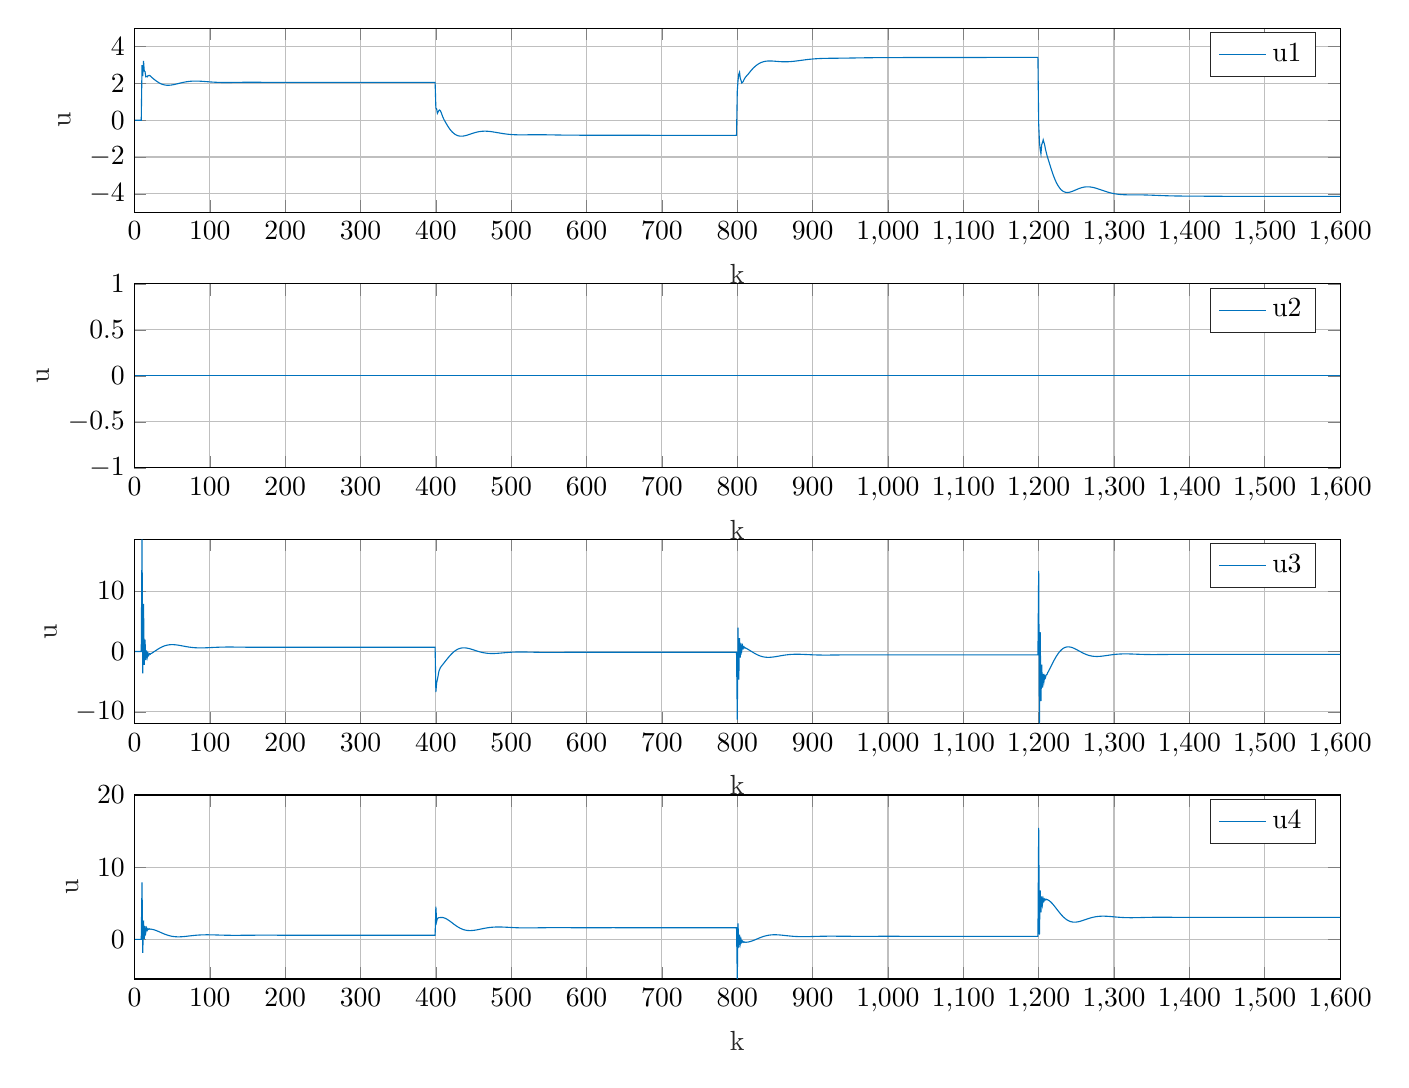
\begin{tikzpicture}

\begin{axis}[%
width=6.028in,
height=0.92in,
at={(1.011in,4.476in)},
scale only axis,
xmin=0,
xmax=1600,
xlabel style={font=\color{white!15!black}},
xlabel={k},
ymin=-5,
ymax=5,
ylabel style={font=\color{white!15!black}},
ylabel={u},
axis background/.style={fill=white},
xmajorgrids,
ymajorgrids,
legend style={legend cell align=left, align=left, draw=white!15!black}
]
\addplot [color=mycolor1]
  table[row sep=crcr]{%
1	0\\
2	0\\
3	0\\
4	0\\
5	0\\
6	0\\
7	0\\
8	0\\
9	0\\
10	2.9925\\
11	2.3995\\
12	3.2256\\
13	2.6804\\
14	2.645\\
15	2.3604\\
16	2.3806\\
17	2.3571\\
18	2.4217\\
19	2.43\\
20	2.4358\\
21	2.4048\\
22	2.3706\\
23	2.3285\\
24	2.2915\\
25	2.2559\\
26	2.2238\\
27	2.1922\\
28	2.1616\\
29	2.1314\\
30	2.1022\\
31	2.0745\\
32	2.0486\\
33	2.0247\\
34	2.0031\\
35	1.9835\\
36	1.9662\\
37	1.9509\\
38	1.9378\\
39	1.9267\\
40	1.9176\\
41	1.9106\\
42	1.9054\\
43	1.902\\
44	1.9003\\
45	1.9003\\
46	1.9017\\
47	1.9045\\
48	1.9085\\
49	1.9137\\
50	1.9199\\
51	1.927\\
52	1.9349\\
53	1.9434\\
54	1.9525\\
55	1.962\\
56	1.9718\\
57	1.9818\\
58	1.9919\\
59	2.0021\\
60	2.0122\\
61	2.0222\\
62	2.032\\
63	2.0415\\
64	2.0507\\
65	2.0594\\
66	2.0678\\
67	2.0757\\
68	2.083\\
69	2.0899\\
70	2.0961\\
71	2.1018\\
72	2.1069\\
73	2.1115\\
74	2.1154\\
75	2.1188\\
76	2.1216\\
77	2.1239\\
78	2.1256\\
79	2.1268\\
80	2.1275\\
81	2.1277\\
82	2.1275\\
83	2.1269\\
84	2.1259\\
85	2.1245\\
86	2.1228\\
87	2.1209\\
88	2.1186\\
89	2.1162\\
90	2.1135\\
91	2.1107\\
92	2.1078\\
93	2.1048\\
94	2.1017\\
95	2.0985\\
96	2.0953\\
97	2.0922\\
98	2.089\\
99	2.0859\\
100	2.0829\\
101	2.08\\
102	2.0771\\
103	2.0744\\
104	2.0718\\
105	2.0693\\
106	2.067\\
107	2.0649\\
108	2.0628\\
109	2.061\\
110	2.0593\\
111	2.0578\\
112	2.0564\\
113	2.0552\\
114	2.0541\\
115	2.0532\\
116	2.0525\\
117	2.0519\\
118	2.0514\\
119	2.0511\\
120	2.0508\\
121	2.0507\\
122	2.0507\\
123	2.0508\\
124	2.051\\
125	2.0513\\
126	2.0516\\
127	2.052\\
128	2.0525\\
129	2.053\\
130	2.0535\\
131	2.0541\\
132	2.0547\\
133	2.0553\\
134	2.0559\\
135	2.0565\\
136	2.0571\\
137	2.0577\\
138	2.0583\\
139	2.0589\\
140	2.0594\\
141	2.0599\\
142	2.0604\\
143	2.0609\\
144	2.0613\\
145	2.0616\\
146	2.062\\
147	2.0623\\
148	2.0626\\
149	2.0628\\
150	2.063\\
151	2.0631\\
152	2.0632\\
153	2.0633\\
154	2.0633\\
155	2.0633\\
156	2.0633\\
157	2.0632\\
158	2.0631\\
159	2.063\\
160	2.0628\\
161	2.0627\\
162	2.0625\\
163	2.0623\\
164	2.062\\
165	2.0618\\
166	2.0615\\
167	2.0613\\
168	2.061\\
169	2.0607\\
170	2.0605\\
171	2.0602\\
172	2.0599\\
173	2.0596\\
174	2.0594\\
175	2.0591\\
176	2.0588\\
177	2.0586\\
178	2.0583\\
179	2.0581\\
180	2.0579\\
181	2.0577\\
182	2.0575\\
183	2.0573\\
184	2.0571\\
185	2.0569\\
186	2.0568\\
187	2.0567\\
188	2.0565\\
189	2.0564\\
190	2.0563\\
191	2.0562\\
192	2.0561\\
193	2.0561\\
194	2.056\\
195	2.056\\
196	2.0559\\
197	2.0559\\
198	2.0559\\
199	2.0558\\
200	2.0558\\
201	2.0558\\
202	2.0558\\
203	2.0558\\
204	2.0558\\
205	2.0559\\
206	2.0559\\
207	2.0559\\
208	2.0559\\
209	2.0559\\
210	2.056\\
211	2.056\\
212	2.056\\
213	2.056\\
214	2.056\\
215	2.0561\\
216	2.0561\\
217	2.0561\\
218	2.0561\\
219	2.0561\\
220	2.0561\\
221	2.0562\\
222	2.0562\\
223	2.0562\\
224	2.0562\\
225	2.0562\\
226	2.0562\\
227	2.0562\\
228	2.0562\\
229	2.0561\\
230	2.0561\\
231	2.0561\\
232	2.0561\\
233	2.0561\\
234	2.0561\\
235	2.056\\
236	2.056\\
237	2.056\\
238	2.056\\
239	2.0559\\
240	2.0559\\
241	2.0559\\
242	2.0559\\
243	2.0558\\
244	2.0558\\
245	2.0558\\
246	2.0557\\
247	2.0557\\
248	2.0557\\
249	2.0557\\
250	2.0556\\
251	2.0556\\
252	2.0556\\
253	2.0555\\
254	2.0555\\
255	2.0555\\
256	2.0555\\
257	2.0555\\
258	2.0554\\
259	2.0554\\
260	2.0554\\
261	2.0554\\
262	2.0554\\
263	2.0553\\
264	2.0553\\
265	2.0553\\
266	2.0553\\
267	2.0553\\
268	2.0553\\
269	2.0553\\
270	2.0553\\
271	2.0553\\
272	2.0552\\
273	2.0552\\
274	2.0552\\
275	2.0552\\
276	2.0552\\
277	2.0552\\
278	2.0552\\
279	2.0552\\
280	2.0552\\
281	2.0552\\
282	2.0552\\
283	2.0552\\
284	2.0552\\
285	2.0552\\
286	2.0552\\
287	2.0552\\
288	2.0552\\
289	2.0552\\
290	2.0552\\
291	2.0552\\
292	2.0552\\
293	2.0552\\
294	2.0552\\
295	2.0552\\
296	2.0552\\
297	2.0552\\
298	2.0552\\
299	2.0552\\
300	2.0552\\
301	2.0552\\
302	2.0552\\
303	2.0551\\
304	2.0551\\
305	2.0551\\
306	2.0551\\
307	2.0551\\
308	2.0551\\
309	2.0551\\
310	2.0551\\
311	2.0551\\
312	2.0551\\
313	2.0551\\
314	2.0551\\
315	2.0551\\
316	2.0551\\
317	2.0551\\
318	2.0551\\
319	2.0551\\
320	2.0551\\
321	2.0551\\
322	2.0551\\
323	2.0551\\
324	2.0551\\
325	2.0551\\
326	2.0551\\
327	2.0551\\
328	2.0551\\
329	2.0551\\
330	2.0551\\
331	2.055\\
332	2.055\\
333	2.055\\
334	2.055\\
335	2.055\\
336	2.055\\
337	2.055\\
338	2.055\\
339	2.055\\
340	2.055\\
341	2.055\\
342	2.055\\
343	2.055\\
344	2.055\\
345	2.055\\
346	2.055\\
347	2.055\\
348	2.055\\
349	2.055\\
350	2.055\\
351	2.055\\
352	2.055\\
353	2.055\\
354	2.055\\
355	2.055\\
356	2.055\\
357	2.055\\
358	2.055\\
359	2.055\\
360	2.055\\
361	2.055\\
362	2.055\\
363	2.055\\
364	2.055\\
365	2.055\\
366	2.055\\
367	2.055\\
368	2.055\\
369	2.055\\
370	2.055\\
371	2.055\\
372	2.055\\
373	2.055\\
374	2.055\\
375	2.055\\
376	2.055\\
377	2.055\\
378	2.055\\
379	2.055\\
380	2.055\\
381	2.055\\
382	2.055\\
383	2.055\\
384	2.055\\
385	2.055\\
386	2.055\\
387	2.055\\
388	2.055\\
389	2.055\\
390	2.055\\
391	2.055\\
392	2.055\\
393	2.055\\
394	2.055\\
395	2.055\\
396	2.055\\
397	2.055\\
398	2.055\\
399	2.055\\
400	0.65847\\
401	0.62581\\
402	0.37197\\
403	0.45098\\
404	0.52733\\
405	0.55922\\
406	0.5172\\
407	0.42284\\
408	0.30966\\
409	0.19969\\
410	0.10357\\
411	0.020186\\
412	-0.054865\\
413	-0.12631\\
414	-0.19633\\
415	-0.26523\\
416	-0.33203\\
417	-0.39564\\
418	-0.45524\\
419	-0.5105\\
420	-0.56137\\
421	-0.60796\\
422	-0.6504\\
423	-0.68876\\
424	-0.72309\\
425	-0.75344\\
426	-0.77987\\
427	-0.80248\\
428	-0.82139\\
429	-0.83677\\
430	-0.84879\\
431	-0.85763\\
432	-0.8635\\
433	-0.86659\\
434	-0.86712\\
435	-0.86529\\
436	-0.86134\\
437	-0.85546\\
438	-0.84789\\
439	-0.83884\\
440	-0.82853\\
441	-0.81714\\
442	-0.8049\\
443	-0.79199\\
444	-0.77859\\
445	-0.76487\\
446	-0.75101\\
447	-0.73715\\
448	-0.72344\\
449	-0.71001\\
450	-0.69698\\
451	-0.68444\\
452	-0.67251\\
453	-0.66126\\
454	-0.65076\\
455	-0.64108\\
456	-0.63226\\
457	-0.62434\\
458	-0.61735\\
459	-0.61131\\
460	-0.60622\\
461	-0.60209\\
462	-0.59891\\
463	-0.59667\\
464	-0.59533\\
465	-0.59488\\
466	-0.59527\\
467	-0.59648\\
468	-0.59845\\
469	-0.60115\\
470	-0.60451\\
471	-0.6085\\
472	-0.61305\\
473	-0.6181\\
474	-0.62362\\
475	-0.62953\\
476	-0.63578\\
477	-0.64233\\
478	-0.6491\\
479	-0.65606\\
480	-0.66314\\
481	-0.67031\\
482	-0.67751\\
483	-0.6847\\
484	-0.69184\\
485	-0.6989\\
486	-0.70582\\
487	-0.71259\\
488	-0.71918\\
489	-0.72555\\
490	-0.73169\\
491	-0.73757\\
492	-0.74317\\
493	-0.7485\\
494	-0.75352\\
495	-0.75824\\
496	-0.76265\\
497	-0.76675\\
498	-0.77053\\
499	-0.774\\
500	-0.77716\\
501	-0.78002\\
502	-0.78259\\
503	-0.78486\\
504	-0.78687\\
505	-0.78861\\
506	-0.7901\\
507	-0.79135\\
508	-0.79238\\
509	-0.7932\\
510	-0.79383\\
511	-0.79429\\
512	-0.79459\\
513	-0.79474\\
514	-0.79476\\
515	-0.79467\\
516	-0.79449\\
517	-0.79422\\
518	-0.79388\\
519	-0.79349\\
520	-0.79306\\
521	-0.7926\\
522	-0.79212\\
523	-0.79164\\
524	-0.79116\\
525	-0.79069\\
526	-0.79024\\
527	-0.78982\\
528	-0.78944\\
529	-0.7891\\
530	-0.78881\\
531	-0.78856\\
532	-0.78837\\
533	-0.78824\\
534	-0.78816\\
535	-0.78815\\
536	-0.78819\\
537	-0.78829\\
538	-0.78846\\
539	-0.78868\\
540	-0.78896\\
541	-0.78929\\
542	-0.78967\\
543	-0.79011\\
544	-0.79059\\
545	-0.79111\\
546	-0.79167\\
547	-0.79227\\
548	-0.7929\\
549	-0.79356\\
550	-0.79425\\
551	-0.79495\\
552	-0.79567\\
553	-0.79641\\
554	-0.79715\\
555	-0.7979\\
556	-0.79865\\
557	-0.7994\\
558	-0.80015\\
559	-0.80089\\
560	-0.80162\\
561	-0.80233\\
562	-0.80303\\
563	-0.80372\\
564	-0.80439\\
565	-0.80503\\
566	-0.80566\\
567	-0.80626\\
568	-0.80684\\
569	-0.80739\\
570	-0.80792\\
571	-0.80842\\
572	-0.80889\\
573	-0.80934\\
574	-0.80976\\
575	-0.81016\\
576	-0.81053\\
577	-0.81088\\
578	-0.8112\\
579	-0.8115\\
580	-0.81178\\
581	-0.81203\\
582	-0.81227\\
583	-0.81248\\
584	-0.81268\\
585	-0.81286\\
586	-0.81302\\
587	-0.81317\\
588	-0.81331\\
589	-0.81343\\
590	-0.81354\\
591	-0.81365\\
592	-0.81374\\
593	-0.81382\\
594	-0.8139\\
595	-0.81397\\
596	-0.81404\\
597	-0.8141\\
598	-0.81417\\
599	-0.81422\\
600	-0.81428\\
601	-0.81434\\
602	-0.81439\\
603	-0.81445\\
604	-0.81451\\
605	-0.81457\\
606	-0.81463\\
607	-0.81469\\
608	-0.81475\\
609	-0.81482\\
610	-0.81489\\
611	-0.81496\\
612	-0.81503\\
613	-0.81511\\
614	-0.81519\\
615	-0.81528\\
616	-0.81536\\
617	-0.81545\\
618	-0.81554\\
619	-0.81563\\
620	-0.81572\\
621	-0.81582\\
622	-0.81592\\
623	-0.81602\\
624	-0.81612\\
625	-0.81622\\
626	-0.81632\\
627	-0.81642\\
628	-0.81652\\
629	-0.81662\\
630	-0.81672\\
631	-0.81682\\
632	-0.81692\\
633	-0.81701\\
634	-0.81711\\
635	-0.8172\\
636	-0.8173\\
637	-0.81739\\
638	-0.81747\\
639	-0.81756\\
640	-0.81765\\
641	-0.81773\\
642	-0.81781\\
643	-0.81788\\
644	-0.81796\\
645	-0.81803\\
646	-0.8181\\
647	-0.81817\\
648	-0.81823\\
649	-0.81829\\
650	-0.81835\\
651	-0.81841\\
652	-0.81846\\
653	-0.81852\\
654	-0.81857\\
655	-0.81861\\
656	-0.81866\\
657	-0.8187\\
658	-0.81874\\
659	-0.81878\\
660	-0.81882\\
661	-0.81886\\
662	-0.81889\\
663	-0.81892\\
664	-0.81895\\
665	-0.81898\\
666	-0.81901\\
667	-0.81904\\
668	-0.81906\\
669	-0.81909\\
670	-0.81911\\
671	-0.81914\\
672	-0.81916\\
673	-0.81918\\
674	-0.81921\\
675	-0.81923\\
676	-0.81925\\
677	-0.81927\\
678	-0.81929\\
679	-0.81931\\
680	-0.81933\\
681	-0.81935\\
682	-0.81937\\
683	-0.81938\\
684	-0.8194\\
685	-0.81942\\
686	-0.81944\\
687	-0.81946\\
688	-0.81948\\
689	-0.81949\\
690	-0.81951\\
691	-0.81953\\
692	-0.81955\\
693	-0.81957\\
694	-0.81958\\
695	-0.8196\\
696	-0.81962\\
697	-0.81964\\
698	-0.81965\\
699	-0.81967\\
700	-0.81969\\
701	-0.8197\\
702	-0.81972\\
703	-0.81974\\
704	-0.81975\\
705	-0.81977\\
706	-0.81978\\
707	-0.8198\\
708	-0.81982\\
709	-0.81983\\
710	-0.81984\\
711	-0.81986\\
712	-0.81987\\
713	-0.81989\\
714	-0.8199\\
715	-0.81991\\
716	-0.81993\\
717	-0.81994\\
718	-0.81995\\
719	-0.81996\\
720	-0.81997\\
721	-0.81999\\
722	-0.82\\
723	-0.82001\\
724	-0.82002\\
725	-0.82003\\
726	-0.82004\\
727	-0.82005\\
728	-0.82005\\
729	-0.82006\\
730	-0.82007\\
731	-0.82008\\
732	-0.82009\\
733	-0.8201\\
734	-0.8201\\
735	-0.82011\\
736	-0.82012\\
737	-0.82012\\
738	-0.82013\\
739	-0.82014\\
740	-0.82014\\
741	-0.82015\\
742	-0.82016\\
743	-0.82016\\
744	-0.82017\\
745	-0.82017\\
746	-0.82018\\
747	-0.82018\\
748	-0.82019\\
749	-0.82019\\
750	-0.8202\\
751	-0.8202\\
752	-0.82021\\
753	-0.82021\\
754	-0.82021\\
755	-0.82022\\
756	-0.82022\\
757	-0.82023\\
758	-0.82023\\
759	-0.82024\\
760	-0.82024\\
761	-0.82024\\
762	-0.82025\\
763	-0.82025\\
764	-0.82025\\
765	-0.82026\\
766	-0.82026\\
767	-0.82026\\
768	-0.82027\\
769	-0.82027\\
770	-0.82027\\
771	-0.82028\\
772	-0.82028\\
773	-0.82028\\
774	-0.82029\\
775	-0.82029\\
776	-0.82029\\
777	-0.8203\\
778	-0.8203\\
779	-0.8203\\
780	-0.82031\\
781	-0.82031\\
782	-0.82031\\
783	-0.82031\\
784	-0.82032\\
785	-0.82032\\
786	-0.82032\\
787	-0.82032\\
788	-0.82033\\
789	-0.82033\\
790	-0.82033\\
791	-0.82033\\
792	-0.82033\\
793	-0.82034\\
794	-0.82034\\
795	-0.82034\\
796	-0.82034\\
797	-0.82034\\
798	-0.82035\\
799	-0.82035\\
800	1.5737\\
801	2.1684\\
802	2.4974\\
803	2.6067\\
804	2.2751\\
805	2.158\\
806	2.0205\\
807	2.063\\
808	2.1156\\
809	2.2122\\
810	2.2817\\
811	2.3458\\
812	2.3923\\
813	2.4385\\
814	2.4835\\
815	2.5326\\
816	2.5829\\
817	2.6341\\
818	2.6837\\
819	2.7315\\
820	2.7768\\
821	2.8198\\
822	2.8605\\
823	2.899\\
824	2.9353\\
825	2.9693\\
826	3.001\\
827	3.0303\\
828	3.0571\\
829	3.0816\\
830	3.1038\\
831	3.1237\\
832	3.1414\\
833	3.157\\
834	3.1706\\
835	3.1823\\
836	3.1922\\
837	3.2004\\
838	3.207\\
839	3.2122\\
840	3.216\\
841	3.2186\\
842	3.2201\\
843	3.2206\\
844	3.2203\\
845	3.2192\\
846	3.2175\\
847	3.2153\\
848	3.2127\\
849	3.2098\\
850	3.2066\\
851	3.2033\\
852	3.1999\\
853	3.1966\\
854	3.1933\\
855	3.1902\\
856	3.1873\\
857	3.1847\\
858	3.1823\\
859	3.1803\\
860	3.1787\\
861	3.1774\\
862	3.1766\\
863	3.1762\\
864	3.1762\\
865	3.1767\\
866	3.1776\\
867	3.1789\\
868	3.1807\\
869	3.1829\\
870	3.1855\\
871	3.1884\\
872	3.1917\\
873	3.1954\\
874	3.1993\\
875	3.2036\\
876	3.2081\\
877	3.2128\\
878	3.2178\\
879	3.2229\\
880	3.2281\\
881	3.2335\\
882	3.239\\
883	3.2445\\
884	3.2501\\
885	3.2556\\
886	3.2612\\
887	3.2667\\
888	3.2722\\
889	3.2776\\
890	3.2828\\
891	3.288\\
892	3.2931\\
893	3.298\\
894	3.3027\\
895	3.3073\\
896	3.3117\\
897	3.3159\\
898	3.3199\\
899	3.3238\\
900	3.3274\\
901	3.3309\\
902	3.3342\\
903	3.3372\\
904	3.3401\\
905	3.3428\\
906	3.3453\\
907	3.3476\\
908	3.3497\\
909	3.3517\\
910	3.3535\\
911	3.3552\\
912	3.3567\\
913	3.3581\\
914	3.3594\\
915	3.3605\\
916	3.3616\\
917	3.3625\\
918	3.3634\\
919	3.3641\\
920	3.3648\\
921	3.3654\\
922	3.366\\
923	3.3665\\
924	3.367\\
925	3.3675\\
926	3.3679\\
927	3.3683\\
928	3.3687\\
929	3.3691\\
930	3.3694\\
931	3.3698\\
932	3.3702\\
933	3.3706\\
934	3.371\\
935	3.3714\\
936	3.3718\\
937	3.3722\\
938	3.3727\\
939	3.3732\\
940	3.3737\\
941	3.3742\\
942	3.3747\\
943	3.3753\\
944	3.3759\\
945	3.3765\\
946	3.3771\\
947	3.3778\\
948	3.3784\\
949	3.3791\\
950	3.3798\\
951	3.3805\\
952	3.3812\\
953	3.3819\\
954	3.3826\\
955	3.3833\\
956	3.384\\
957	3.3848\\
958	3.3855\\
959	3.3862\\
960	3.3869\\
961	3.3876\\
962	3.3883\\
963	3.389\\
964	3.3897\\
965	3.3903\\
966	3.391\\
967	3.3916\\
968	3.3922\\
969	3.3929\\
970	3.3934\\
971	3.394\\
972	3.3946\\
973	3.3951\\
974	3.3956\\
975	3.3961\\
976	3.3966\\
977	3.397\\
978	3.3975\\
979	3.3979\\
980	3.3983\\
981	3.3987\\
982	3.399\\
983	3.3994\\
984	3.3997\\
985	3.4\\
986	3.4003\\
987	3.4006\\
988	3.4009\\
989	3.4012\\
990	3.4014\\
991	3.4016\\
992	3.4019\\
993	3.4021\\
994	3.4023\\
995	3.4025\\
996	3.4027\\
997	3.4029\\
998	3.403\\
999	3.4032\\
1000	3.4034\\
1001	3.4035\\
1002	3.4037\\
1003	3.4038\\
1004	3.404\\
1005	3.4041\\
1006	3.4043\\
1007	3.4044\\
1008	3.4045\\
1009	3.4047\\
1010	3.4048\\
1011	3.4049\\
1012	3.4051\\
1013	3.4052\\
1014	3.4053\\
1015	3.4054\\
1016	3.4056\\
1017	3.4057\\
1018	3.4058\\
1019	3.406\\
1020	3.4061\\
1021	3.4062\\
1022	3.4063\\
1023	3.4065\\
1024	3.4066\\
1025	3.4067\\
1026	3.4068\\
1027	3.4069\\
1028	3.4071\\
1029	3.4072\\
1030	3.4073\\
1031	3.4074\\
1032	3.4075\\
1033	3.4076\\
1034	3.4078\\
1035	3.4079\\
1036	3.408\\
1037	3.4081\\
1038	3.4082\\
1039	3.4083\\
1040	3.4084\\
1041	3.4085\\
1042	3.4086\\
1043	3.4087\\
1044	3.4088\\
1045	3.4089\\
1046	3.409\\
1047	3.409\\
1048	3.4091\\
1049	3.4092\\
1050	3.4093\\
1051	3.4094\\
1052	3.4094\\
1053	3.4095\\
1054	3.4096\\
1055	3.4096\\
1056	3.4097\\
1057	3.4098\\
1058	3.4098\\
1059	3.4099\\
1060	3.41\\
1061	3.41\\
1062	3.4101\\
1063	3.4101\\
1064	3.4102\\
1065	3.4102\\
1066	3.4103\\
1067	3.4103\\
1068	3.4104\\
1069	3.4104\\
1070	3.4104\\
1071	3.4105\\
1072	3.4105\\
1073	3.4106\\
1074	3.4106\\
1075	3.4106\\
1076	3.4107\\
1077	3.4107\\
1078	3.4107\\
1079	3.4108\\
1080	3.4108\\
1081	3.4108\\
1082	3.4109\\
1083	3.4109\\
1084	3.4109\\
1085	3.4109\\
1086	3.411\\
1087	3.411\\
1088	3.411\\
1089	3.4111\\
1090	3.4111\\
1091	3.4111\\
1092	3.4111\\
1093	3.4112\\
1094	3.4112\\
1095	3.4112\\
1096	3.4112\\
1097	3.4113\\
1098	3.4113\\
1099	3.4113\\
1100	3.4113\\
1101	3.4114\\
1102	3.4114\\
1103	3.4114\\
1104	3.4114\\
1105	3.4114\\
1106	3.4115\\
1107	3.4115\\
1108	3.4115\\
1109	3.4115\\
1110	3.4115\\
1111	3.4116\\
1112	3.4116\\
1113	3.4116\\
1114	3.4116\\
1115	3.4116\\
1116	3.4116\\
1117	3.4117\\
1118	3.4117\\
1119	3.4117\\
1120	3.4117\\
1121	3.4117\\
1122	3.4117\\
1123	3.4118\\
1124	3.4118\\
1125	3.4118\\
1126	3.4118\\
1127	3.4118\\
1128	3.4118\\
1129	3.4118\\
1130	3.4118\\
1131	3.4119\\
1132	3.4119\\
1133	3.4119\\
1134	3.4119\\
1135	3.4119\\
1136	3.4119\\
1137	3.4119\\
1138	3.4119\\
1139	3.4119\\
1140	3.4119\\
1141	3.412\\
1142	3.412\\
1143	3.412\\
1144	3.412\\
1145	3.412\\
1146	3.412\\
1147	3.412\\
1148	3.412\\
1149	3.412\\
1150	3.412\\
1151	3.412\\
1152	3.412\\
1153	3.4121\\
1154	3.4121\\
1155	3.4121\\
1156	3.4121\\
1157	3.4121\\
1158	3.4121\\
1159	3.4121\\
1160	3.4121\\
1161	3.4121\\
1162	3.4121\\
1163	3.4121\\
1164	3.4121\\
1165	3.4121\\
1166	3.4121\\
1167	3.4121\\
1168	3.4121\\
1169	3.4121\\
1170	3.4121\\
1171	3.4121\\
1172	3.4122\\
1173	3.4122\\
1174	3.4122\\
1175	3.4122\\
1176	3.4122\\
1177	3.4122\\
1178	3.4122\\
1179	3.4122\\
1180	3.4122\\
1181	3.4122\\
1182	3.4122\\
1183	3.4122\\
1184	3.4122\\
1185	3.4122\\
1186	3.4122\\
1187	3.4122\\
1188	3.4122\\
1189	3.4122\\
1190	3.4122\\
1191	3.4122\\
1192	3.4122\\
1193	3.4122\\
1194	3.4122\\
1195	3.4122\\
1196	3.4122\\
1197	3.4122\\
1198	3.4122\\
1199	3.4122\\
1200	-0.17875\\
1201	-1.17\\
1202	-1.6032\\
1203	-1.8323\\
1204	-1.3298\\
1205	-1.2215\\
1206	-1.0646\\
1207	-1.2065\\
1208	-1.3539\\
1209	-1.5733\\
1210	-1.7453\\
1211	-1.9092\\
1212	-2.0434\\
1213	-2.1764\\
1214	-2.3051\\
1215	-2.4381\\
1216	-2.57\\
1217	-2.7003\\
1218	-2.8249\\
1219	-2.9434\\
1220	-3.0546\\
1221	-3.1587\\
1222	-3.2559\\
1223	-3.3461\\
1224	-3.4295\\
1225	-3.5059\\
1226	-3.5752\\
1227	-3.6376\\
1228	-3.6931\\
1229	-3.742\\
1230	-3.7843\\
1231	-3.8204\\
1232	-3.8507\\
1233	-3.8753\\
1234	-3.8946\\
1235	-3.9089\\
1236	-3.9186\\
1237	-3.9241\\
1238	-3.9257\\
1239	-3.9238\\
1240	-3.9188\\
1241	-3.911\\
1242	-3.9008\\
1243	-3.8886\\
1244	-3.8747\\
1245	-3.8593\\
1246	-3.8429\\
1247	-3.8258\\
1248	-3.8082\\
1249	-3.7904\\
1250	-3.7726\\
1251	-3.7551\\
1252	-3.738\\
1253	-3.7216\\
1254	-3.7061\\
1255	-3.6915\\
1256	-3.6781\\
1257	-3.6658\\
1258	-3.6549\\
1259	-3.6454\\
1260	-3.6373\\
1261	-3.6306\\
1262	-3.6255\\
1263	-3.6219\\
1264	-3.6198\\
1265	-3.6191\\
1266	-3.6199\\
1267	-3.6221\\
1268	-3.6257\\
1269	-3.6305\\
1270	-3.6366\\
1271	-3.6438\\
1272	-3.6521\\
1273	-3.6614\\
1274	-3.6716\\
1275	-3.6826\\
1276	-3.6943\\
1277	-3.7067\\
1278	-3.7195\\
1279	-3.7329\\
1280	-3.7466\\
1281	-3.7605\\
1282	-3.7746\\
1283	-3.7889\\
1284	-3.8032\\
1285	-3.8174\\
1286	-3.8315\\
1287	-3.8454\\
1288	-3.8591\\
1289	-3.8725\\
1290	-3.8855\\
1291	-3.8981\\
1292	-3.9104\\
1293	-3.9221\\
1294	-3.9334\\
1295	-3.9442\\
1296	-3.9544\\
1297	-3.9641\\
1298	-3.9732\\
1299	-3.9818\\
1300	-3.9898\\
1301	-3.9972\\
1302	-4.0041\\
1303	-4.0105\\
1304	-4.0163\\
1305	-4.0216\\
1306	-4.0265\\
1307	-4.0308\\
1308	-4.0347\\
1309	-4.0381\\
1310	-4.0412\\
1311	-4.0438\\
1312	-4.0461\\
1313	-4.0481\\
1314	-4.0498\\
1315	-4.0512\\
1316	-4.0524\\
1317	-4.0533\\
1318	-4.0541\\
1319	-4.0546\\
1320	-4.0551\\
1321	-4.0554\\
1322	-4.0556\\
1323	-4.0558\\
1324	-4.0559\\
1325	-4.0559\\
1326	-4.056\\
1327	-4.056\\
1328	-4.056\\
1329	-4.0561\\
1330	-4.0562\\
1331	-4.0564\\
1332	-4.0566\\
1333	-4.0569\\
1334	-4.0573\\
1335	-4.0577\\
1336	-4.0582\\
1337	-4.0588\\
1338	-4.0595\\
1339	-4.0603\\
1340	-4.0611\\
1341	-4.0621\\
1342	-4.0631\\
1343	-4.0642\\
1344	-4.0654\\
1345	-4.0667\\
1346	-4.068\\
1347	-4.0693\\
1348	-4.0708\\
1349	-4.0723\\
1350	-4.0738\\
1351	-4.0754\\
1352	-4.077\\
1353	-4.0786\\
1354	-4.0802\\
1355	-4.0819\\
1356	-4.0836\\
1357	-4.0852\\
1358	-4.0869\\
1359	-4.0886\\
1360	-4.0902\\
1361	-4.0918\\
1362	-4.0934\\
1363	-4.095\\
1364	-4.0965\\
1365	-4.098\\
1366	-4.0995\\
1367	-4.1009\\
1368	-4.1023\\
1369	-4.1036\\
1370	-4.1049\\
1371	-4.1062\\
1372	-4.1074\\
1373	-4.1085\\
1374	-4.1096\\
1375	-4.1106\\
1376	-4.1116\\
1377	-4.1126\\
1378	-4.1135\\
1379	-4.1143\\
1380	-4.1151\\
1381	-4.1159\\
1382	-4.1166\\
1383	-4.1172\\
1384	-4.1179\\
1385	-4.1185\\
1386	-4.119\\
1387	-4.1195\\
1388	-4.12\\
1389	-4.1205\\
1390	-4.1209\\
1391	-4.1213\\
1392	-4.1217\\
1393	-4.1221\\
1394	-4.1224\\
1395	-4.1227\\
1396	-4.123\\
1397	-4.1233\\
1398	-4.1236\\
1399	-4.1239\\
1400	-4.1241\\
1401	-4.1244\\
1402	-4.1246\\
1403	-4.1249\\
1404	-4.1251\\
1405	-4.1254\\
1406	-4.1256\\
1407	-4.1258\\
1408	-4.1261\\
1409	-4.1263\\
1410	-4.1265\\
1411	-4.1268\\
1412	-4.127\\
1413	-4.1272\\
1414	-4.1275\\
1415	-4.1277\\
1416	-4.128\\
1417	-4.1282\\
1418	-4.1285\\
1419	-4.1287\\
1420	-4.129\\
1421	-4.1292\\
1422	-4.1295\\
1423	-4.1297\\
1424	-4.13\\
1425	-4.1302\\
1426	-4.1305\\
1427	-4.1307\\
1428	-4.131\\
1429	-4.1312\\
1430	-4.1315\\
1431	-4.1317\\
1432	-4.132\\
1433	-4.1322\\
1434	-4.1325\\
1435	-4.1327\\
1436	-4.1329\\
1437	-4.1332\\
1438	-4.1334\\
1439	-4.1336\\
1440	-4.1338\\
1441	-4.134\\
1442	-4.1342\\
1443	-4.1344\\
1444	-4.1346\\
1445	-4.1348\\
1446	-4.135\\
1447	-4.1352\\
1448	-4.1353\\
1449	-4.1355\\
1450	-4.1357\\
1451	-4.1358\\
1452	-4.136\\
1453	-4.1361\\
1454	-4.1363\\
1455	-4.1364\\
1456	-4.1365\\
1457	-4.1366\\
1458	-4.1368\\
1459	-4.1369\\
1460	-4.137\\
1461	-4.1371\\
1462	-4.1372\\
1463	-4.1373\\
1464	-4.1374\\
1465	-4.1375\\
1466	-4.1376\\
1467	-4.1377\\
1468	-4.1377\\
1469	-4.1378\\
1470	-4.1379\\
1471	-4.138\\
1472	-4.1381\\
1473	-4.1381\\
1474	-4.1382\\
1475	-4.1383\\
1476	-4.1383\\
1477	-4.1384\\
1478	-4.1385\\
1479	-4.1385\\
1480	-4.1386\\
1481	-4.1386\\
1482	-4.1387\\
1483	-4.1387\\
1484	-4.1388\\
1485	-4.1389\\
1486	-4.1389\\
1487	-4.139\\
1488	-4.139\\
1489	-4.1391\\
1490	-4.1391\\
1491	-4.1392\\
1492	-4.1392\\
1493	-4.1393\\
1494	-4.1393\\
1495	-4.1394\\
1496	-4.1394\\
1497	-4.1395\\
1498	-4.1395\\
1499	-4.1396\\
1500	-4.1396\\
1501	-4.1397\\
1502	-4.1397\\
1503	-4.1397\\
1504	-4.1398\\
1505	-4.1398\\
1506	-4.1399\\
1507	-4.1399\\
1508	-4.14\\
1509	-4.14\\
1510	-4.14\\
1511	-4.1401\\
1512	-4.1401\\
1513	-4.1401\\
1514	-4.1402\\
1515	-4.1402\\
1516	-4.1403\\
1517	-4.1403\\
1518	-4.1403\\
1519	-4.1403\\
1520	-4.1404\\
1521	-4.1404\\
1522	-4.1404\\
1523	-4.1405\\
1524	-4.1405\\
1525	-4.1405\\
1526	-4.1406\\
1527	-4.1406\\
1528	-4.1406\\
1529	-4.1406\\
1530	-4.1407\\
1531	-4.1407\\
1532	-4.1407\\
1533	-4.1407\\
1534	-4.1407\\
1535	-4.1408\\
1536	-4.1408\\
1537	-4.1408\\
1538	-4.1408\\
1539	-4.1408\\
1540	-4.1409\\
1541	-4.1409\\
1542	-4.1409\\
1543	-4.1409\\
1544	-4.1409\\
1545	-4.1409\\
1546	-4.141\\
1547	-4.141\\
1548	-4.141\\
1549	-4.141\\
1550	-4.141\\
1551	-4.141\\
1552	-4.141\\
1553	-4.1411\\
1554	-4.1411\\
1555	-4.1411\\
1556	-4.1411\\
1557	-4.1411\\
1558	-4.1411\\
1559	-4.1411\\
1560	-4.1411\\
1561	-4.1411\\
1562	-4.1412\\
1563	-4.1412\\
1564	-4.1412\\
1565	-4.1412\\
1566	-4.1412\\
1567	-4.1412\\
1568	-4.1412\\
1569	-4.1412\\
1570	-4.1412\\
1571	-4.1412\\
1572	-4.1413\\
1573	-4.1413\\
1574	-4.1413\\
1575	-4.1413\\
1576	-4.1413\\
1577	-4.1413\\
1578	-4.1413\\
1579	-4.1413\\
1580	-4.1413\\
1581	-4.1413\\
1582	-4.1413\\
1583	-4.1413\\
1584	-4.1414\\
1585	-4.1414\\
1586	-4.1414\\
1587	-4.1414\\
1588	-4.1414\\
1589	-4.1414\\
1590	-4.1414\\
1591	-4.1414\\
1592	-4.1414\\
1593	-4.1414\\
1594	-4.1414\\
1595	-4.1414\\
1596	-4.1414\\
1597	-4.1414\\
1598	-4.1414\\
1599	-4.1414\\
1600	-4.1414\\
};
\addlegendentry{u1}

\end{axis}

\begin{axis}[%
width=6.028in,
height=0.92in,
at={(1.011in,3.198in)},
scale only axis,
xmin=0,
xmax=1600,
xlabel style={font=\color{white!15!black}},
xlabel={k},
ymin=-1,
ymax=1,
ylabel style={font=\color{white!15!black}},
ylabel={u},
axis background/.style={fill=white},
xmajorgrids,
ymajorgrids,
legend style={legend cell align=left, align=left, draw=white!15!black}
]
\addplot [color=mycolor1]
  table[row sep=crcr]{%
1	0\\
2	0\\
3	0\\
4	0\\
5	0\\
6	0\\
7	0\\
8	0\\
9	0\\
10	0\\
11	0\\
12	0\\
13	0\\
14	0\\
15	0\\
16	0\\
17	0\\
18	0\\
19	0\\
20	0\\
21	0\\
22	0\\
23	0\\
24	0\\
25	0\\
26	0\\
27	0\\
28	0\\
29	0\\
30	0\\
31	0\\
32	0\\
33	0\\
34	0\\
35	0\\
36	0\\
37	0\\
38	0\\
39	0\\
40	0\\
41	0\\
42	0\\
43	0\\
44	0\\
45	0\\
46	0\\
47	0\\
48	0\\
49	0\\
50	0\\
51	0\\
52	0\\
53	0\\
54	0\\
55	0\\
56	0\\
57	0\\
58	0\\
59	0\\
60	0\\
61	0\\
62	0\\
63	0\\
64	0\\
65	0\\
66	0\\
67	0\\
68	0\\
69	0\\
70	0\\
71	0\\
72	0\\
73	0\\
74	0\\
75	0\\
76	0\\
77	0\\
78	0\\
79	0\\
80	0\\
81	0\\
82	0\\
83	0\\
84	0\\
85	0\\
86	0\\
87	0\\
88	0\\
89	0\\
90	0\\
91	0\\
92	0\\
93	0\\
94	0\\
95	0\\
96	0\\
97	0\\
98	0\\
99	0\\
100	0\\
101	0\\
102	0\\
103	0\\
104	0\\
105	0\\
106	0\\
107	0\\
108	0\\
109	0\\
110	0\\
111	0\\
112	0\\
113	0\\
114	0\\
115	0\\
116	0\\
117	0\\
118	0\\
119	0\\
120	0\\
121	0\\
122	0\\
123	0\\
124	0\\
125	0\\
126	0\\
127	0\\
128	0\\
129	0\\
130	0\\
131	0\\
132	0\\
133	0\\
134	0\\
135	0\\
136	0\\
137	0\\
138	0\\
139	0\\
140	0\\
141	0\\
142	0\\
143	0\\
144	0\\
145	0\\
146	0\\
147	0\\
148	0\\
149	0\\
150	0\\
151	0\\
152	0\\
153	0\\
154	0\\
155	0\\
156	0\\
157	0\\
158	0\\
159	0\\
160	0\\
161	0\\
162	0\\
163	0\\
164	0\\
165	0\\
166	0\\
167	0\\
168	0\\
169	0\\
170	0\\
171	0\\
172	0\\
173	0\\
174	0\\
175	0\\
176	0\\
177	0\\
178	0\\
179	0\\
180	0\\
181	0\\
182	0\\
183	0\\
184	0\\
185	0\\
186	0\\
187	0\\
188	0\\
189	0\\
190	0\\
191	0\\
192	0\\
193	0\\
194	0\\
195	0\\
196	0\\
197	0\\
198	0\\
199	0\\
200	0\\
201	0\\
202	0\\
203	0\\
204	0\\
205	0\\
206	0\\
207	0\\
208	0\\
209	0\\
210	0\\
211	0\\
212	0\\
213	0\\
214	0\\
215	0\\
216	0\\
217	0\\
218	0\\
219	0\\
220	0\\
221	0\\
222	0\\
223	0\\
224	0\\
225	0\\
226	0\\
227	0\\
228	0\\
229	0\\
230	0\\
231	0\\
232	0\\
233	0\\
234	0\\
235	0\\
236	0\\
237	0\\
238	0\\
239	0\\
240	0\\
241	0\\
242	0\\
243	0\\
244	0\\
245	0\\
246	0\\
247	0\\
248	0\\
249	0\\
250	0\\
251	0\\
252	0\\
253	0\\
254	0\\
255	0\\
256	0\\
257	0\\
258	0\\
259	0\\
260	0\\
261	0\\
262	0\\
263	0\\
264	0\\
265	0\\
266	0\\
267	0\\
268	0\\
269	0\\
270	0\\
271	0\\
272	0\\
273	0\\
274	0\\
275	0\\
276	0\\
277	0\\
278	0\\
279	0\\
280	0\\
281	0\\
282	0\\
283	0\\
284	0\\
285	0\\
286	0\\
287	0\\
288	0\\
289	0\\
290	0\\
291	0\\
292	0\\
293	0\\
294	0\\
295	0\\
296	0\\
297	0\\
298	0\\
299	0\\
300	0\\
301	0\\
302	0\\
303	0\\
304	0\\
305	0\\
306	0\\
307	0\\
308	0\\
309	0\\
310	0\\
311	0\\
312	0\\
313	0\\
314	0\\
315	0\\
316	0\\
317	0\\
318	0\\
319	0\\
320	0\\
321	0\\
322	0\\
323	0\\
324	0\\
325	0\\
326	0\\
327	0\\
328	0\\
329	0\\
330	0\\
331	0\\
332	0\\
333	0\\
334	0\\
335	0\\
336	0\\
337	0\\
338	0\\
339	0\\
340	0\\
341	0\\
342	0\\
343	0\\
344	0\\
345	0\\
346	0\\
347	0\\
348	0\\
349	0\\
350	0\\
351	0\\
352	0\\
353	0\\
354	0\\
355	0\\
356	0\\
357	0\\
358	0\\
359	0\\
360	0\\
361	0\\
362	0\\
363	0\\
364	0\\
365	0\\
366	0\\
367	0\\
368	0\\
369	0\\
370	0\\
371	0\\
372	0\\
373	0\\
374	0\\
375	0\\
376	0\\
377	0\\
378	0\\
379	0\\
380	0\\
381	0\\
382	0\\
383	0\\
384	0\\
385	0\\
386	0\\
387	0\\
388	0\\
389	0\\
390	0\\
391	0\\
392	0\\
393	0\\
394	0\\
395	0\\
396	0\\
397	0\\
398	0\\
399	0\\
400	0\\
401	0\\
402	0\\
403	0\\
404	0\\
405	0\\
406	0\\
407	0\\
408	0\\
409	0\\
410	0\\
411	0\\
412	0\\
413	0\\
414	0\\
415	0\\
416	0\\
417	0\\
418	0\\
419	0\\
420	0\\
421	0\\
422	0\\
423	0\\
424	0\\
425	0\\
426	0\\
427	0\\
428	0\\
429	0\\
430	0\\
431	0\\
432	0\\
433	0\\
434	0\\
435	0\\
436	0\\
437	0\\
438	0\\
439	0\\
440	0\\
441	0\\
442	0\\
443	0\\
444	0\\
445	0\\
446	0\\
447	0\\
448	0\\
449	0\\
450	0\\
451	0\\
452	0\\
453	0\\
454	0\\
455	0\\
456	0\\
457	0\\
458	0\\
459	0\\
460	0\\
461	0\\
462	0\\
463	0\\
464	0\\
465	0\\
466	0\\
467	0\\
468	0\\
469	0\\
470	0\\
471	0\\
472	0\\
473	0\\
474	0\\
475	0\\
476	0\\
477	0\\
478	0\\
479	0\\
480	0\\
481	0\\
482	0\\
483	0\\
484	0\\
485	0\\
486	0\\
487	0\\
488	0\\
489	0\\
490	0\\
491	0\\
492	0\\
493	0\\
494	0\\
495	0\\
496	0\\
497	0\\
498	0\\
499	0\\
500	0\\
501	0\\
502	0\\
503	0\\
504	0\\
505	0\\
506	0\\
507	0\\
508	0\\
509	0\\
510	0\\
511	0\\
512	0\\
513	0\\
514	0\\
515	0\\
516	0\\
517	0\\
518	0\\
519	0\\
520	0\\
521	0\\
522	0\\
523	0\\
524	0\\
525	0\\
526	0\\
527	0\\
528	0\\
529	0\\
530	0\\
531	0\\
532	0\\
533	0\\
534	0\\
535	0\\
536	0\\
537	0\\
538	0\\
539	0\\
540	0\\
541	0\\
542	0\\
543	0\\
544	0\\
545	0\\
546	0\\
547	0\\
548	0\\
549	0\\
550	0\\
551	0\\
552	0\\
553	0\\
554	0\\
555	0\\
556	0\\
557	0\\
558	0\\
559	0\\
560	0\\
561	0\\
562	0\\
563	0\\
564	0\\
565	0\\
566	0\\
567	0\\
568	0\\
569	0\\
570	0\\
571	0\\
572	0\\
573	0\\
574	0\\
575	0\\
576	0\\
577	0\\
578	0\\
579	0\\
580	0\\
581	0\\
582	0\\
583	0\\
584	0\\
585	0\\
586	0\\
587	0\\
588	0\\
589	0\\
590	0\\
591	0\\
592	0\\
593	0\\
594	0\\
595	0\\
596	0\\
597	0\\
598	0\\
599	0\\
600	0\\
601	0\\
602	0\\
603	0\\
604	0\\
605	0\\
606	0\\
607	0\\
608	0\\
609	0\\
610	0\\
611	0\\
612	0\\
613	0\\
614	0\\
615	0\\
616	0\\
617	0\\
618	0\\
619	0\\
620	0\\
621	0\\
622	0\\
623	0\\
624	0\\
625	0\\
626	0\\
627	0\\
628	0\\
629	0\\
630	0\\
631	0\\
632	0\\
633	0\\
634	0\\
635	0\\
636	0\\
637	0\\
638	0\\
639	0\\
640	0\\
641	0\\
642	0\\
643	0\\
644	0\\
645	0\\
646	0\\
647	0\\
648	0\\
649	0\\
650	0\\
651	0\\
652	0\\
653	0\\
654	0\\
655	0\\
656	0\\
657	0\\
658	0\\
659	0\\
660	0\\
661	0\\
662	0\\
663	0\\
664	0\\
665	0\\
666	0\\
667	0\\
668	0\\
669	0\\
670	0\\
671	0\\
672	0\\
673	0\\
674	0\\
675	0\\
676	0\\
677	0\\
678	0\\
679	0\\
680	0\\
681	0\\
682	0\\
683	0\\
684	0\\
685	0\\
686	0\\
687	0\\
688	0\\
689	0\\
690	0\\
691	0\\
692	0\\
693	0\\
694	0\\
695	0\\
696	0\\
697	0\\
698	0\\
699	0\\
700	0\\
701	0\\
702	0\\
703	0\\
704	0\\
705	0\\
706	0\\
707	0\\
708	0\\
709	0\\
710	0\\
711	0\\
712	0\\
713	0\\
714	0\\
715	0\\
716	0\\
717	0\\
718	0\\
719	0\\
720	0\\
721	0\\
722	0\\
723	0\\
724	0\\
725	0\\
726	0\\
727	0\\
728	0\\
729	0\\
730	0\\
731	0\\
732	0\\
733	0\\
734	0\\
735	0\\
736	0\\
737	0\\
738	0\\
739	0\\
740	0\\
741	0\\
742	0\\
743	0\\
744	0\\
745	0\\
746	0\\
747	0\\
748	0\\
749	0\\
750	0\\
751	0\\
752	0\\
753	0\\
754	0\\
755	0\\
756	0\\
757	0\\
758	0\\
759	0\\
760	0\\
761	0\\
762	0\\
763	0\\
764	0\\
765	0\\
766	0\\
767	0\\
768	0\\
769	0\\
770	0\\
771	0\\
772	0\\
773	0\\
774	0\\
775	0\\
776	0\\
777	0\\
778	0\\
779	0\\
780	0\\
781	0\\
782	0\\
783	0\\
784	0\\
785	0\\
786	0\\
787	0\\
788	0\\
789	0\\
790	0\\
791	0\\
792	0\\
793	0\\
794	0\\
795	0\\
796	0\\
797	0\\
798	0\\
799	0\\
800	0\\
801	0\\
802	0\\
803	0\\
804	0\\
805	0\\
806	0\\
807	0\\
808	0\\
809	0\\
810	0\\
811	0\\
812	0\\
813	0\\
814	0\\
815	0\\
816	0\\
817	0\\
818	0\\
819	0\\
820	0\\
821	0\\
822	0\\
823	0\\
824	0\\
825	0\\
826	0\\
827	0\\
828	0\\
829	0\\
830	0\\
831	0\\
832	0\\
833	0\\
834	0\\
835	0\\
836	0\\
837	0\\
838	0\\
839	0\\
840	0\\
841	0\\
842	0\\
843	0\\
844	0\\
845	0\\
846	0\\
847	0\\
848	0\\
849	0\\
850	0\\
851	0\\
852	0\\
853	0\\
854	0\\
855	0\\
856	0\\
857	0\\
858	0\\
859	0\\
860	0\\
861	0\\
862	0\\
863	0\\
864	0\\
865	0\\
866	0\\
867	0\\
868	0\\
869	0\\
870	0\\
871	0\\
872	0\\
873	0\\
874	0\\
875	0\\
876	0\\
877	0\\
878	0\\
879	0\\
880	0\\
881	0\\
882	0\\
883	0\\
884	0\\
885	0\\
886	0\\
887	0\\
888	0\\
889	0\\
890	0\\
891	0\\
892	0\\
893	0\\
894	0\\
895	0\\
896	0\\
897	0\\
898	0\\
899	0\\
900	0\\
901	0\\
902	0\\
903	0\\
904	0\\
905	0\\
906	0\\
907	0\\
908	0\\
909	0\\
910	0\\
911	0\\
912	0\\
913	0\\
914	0\\
915	0\\
916	0\\
917	0\\
918	0\\
919	0\\
920	0\\
921	0\\
922	0\\
923	0\\
924	0\\
925	0\\
926	0\\
927	0\\
928	0\\
929	0\\
930	0\\
931	0\\
932	0\\
933	0\\
934	0\\
935	0\\
936	0\\
937	0\\
938	0\\
939	0\\
940	0\\
941	0\\
942	0\\
943	0\\
944	0\\
945	0\\
946	0\\
947	0\\
948	0\\
949	0\\
950	0\\
951	0\\
952	0\\
953	0\\
954	0\\
955	0\\
956	0\\
957	0\\
958	0\\
959	0\\
960	0\\
961	0\\
962	0\\
963	0\\
964	0\\
965	0\\
966	0\\
967	0\\
968	0\\
969	0\\
970	0\\
971	0\\
972	0\\
973	0\\
974	0\\
975	0\\
976	0\\
977	0\\
978	0\\
979	0\\
980	0\\
981	0\\
982	0\\
983	0\\
984	0\\
985	0\\
986	0\\
987	0\\
988	0\\
989	0\\
990	0\\
991	0\\
992	0\\
993	0\\
994	0\\
995	0\\
996	0\\
997	0\\
998	0\\
999	0\\
1000	0\\
1001	0\\
1002	0\\
1003	0\\
1004	0\\
1005	0\\
1006	0\\
1007	0\\
1008	0\\
1009	0\\
1010	0\\
1011	0\\
1012	0\\
1013	0\\
1014	0\\
1015	0\\
1016	0\\
1017	0\\
1018	0\\
1019	0\\
1020	0\\
1021	0\\
1022	0\\
1023	0\\
1024	0\\
1025	0\\
1026	0\\
1027	0\\
1028	0\\
1029	0\\
1030	0\\
1031	0\\
1032	0\\
1033	0\\
1034	0\\
1035	0\\
1036	0\\
1037	0\\
1038	0\\
1039	0\\
1040	0\\
1041	0\\
1042	0\\
1043	0\\
1044	0\\
1045	0\\
1046	0\\
1047	0\\
1048	0\\
1049	0\\
1050	0\\
1051	0\\
1052	0\\
1053	0\\
1054	0\\
1055	0\\
1056	0\\
1057	0\\
1058	0\\
1059	0\\
1060	0\\
1061	0\\
1062	0\\
1063	0\\
1064	0\\
1065	0\\
1066	0\\
1067	0\\
1068	0\\
1069	0\\
1070	0\\
1071	0\\
1072	0\\
1073	0\\
1074	0\\
1075	0\\
1076	0\\
1077	0\\
1078	0\\
1079	0\\
1080	0\\
1081	0\\
1082	0\\
1083	0\\
1084	0\\
1085	0\\
1086	0\\
1087	0\\
1088	0\\
1089	0\\
1090	0\\
1091	0\\
1092	0\\
1093	0\\
1094	0\\
1095	0\\
1096	0\\
1097	0\\
1098	0\\
1099	0\\
1100	0\\
1101	0\\
1102	0\\
1103	0\\
1104	0\\
1105	0\\
1106	0\\
1107	0\\
1108	0\\
1109	0\\
1110	0\\
1111	0\\
1112	0\\
1113	0\\
1114	0\\
1115	0\\
1116	0\\
1117	0\\
1118	0\\
1119	0\\
1120	0\\
1121	0\\
1122	0\\
1123	0\\
1124	0\\
1125	0\\
1126	0\\
1127	0\\
1128	0\\
1129	0\\
1130	0\\
1131	0\\
1132	0\\
1133	0\\
1134	0\\
1135	0\\
1136	0\\
1137	0\\
1138	0\\
1139	0\\
1140	0\\
1141	0\\
1142	0\\
1143	0\\
1144	0\\
1145	0\\
1146	0\\
1147	0\\
1148	0\\
1149	0\\
1150	0\\
1151	0\\
1152	0\\
1153	0\\
1154	0\\
1155	0\\
1156	0\\
1157	0\\
1158	0\\
1159	0\\
1160	0\\
1161	0\\
1162	0\\
1163	0\\
1164	0\\
1165	0\\
1166	0\\
1167	0\\
1168	0\\
1169	0\\
1170	0\\
1171	0\\
1172	0\\
1173	0\\
1174	0\\
1175	0\\
1176	0\\
1177	0\\
1178	0\\
1179	0\\
1180	0\\
1181	0\\
1182	0\\
1183	0\\
1184	0\\
1185	0\\
1186	0\\
1187	0\\
1188	0\\
1189	0\\
1190	0\\
1191	0\\
1192	0\\
1193	0\\
1194	0\\
1195	0\\
1196	0\\
1197	0\\
1198	0\\
1199	0\\
1200	0\\
1201	0\\
1202	0\\
1203	0\\
1204	0\\
1205	0\\
1206	0\\
1207	0\\
1208	0\\
1209	0\\
1210	0\\
1211	0\\
1212	0\\
1213	0\\
1214	0\\
1215	0\\
1216	0\\
1217	0\\
1218	0\\
1219	0\\
1220	0\\
1221	0\\
1222	0\\
1223	0\\
1224	0\\
1225	0\\
1226	0\\
1227	0\\
1228	0\\
1229	0\\
1230	0\\
1231	0\\
1232	0\\
1233	0\\
1234	0\\
1235	0\\
1236	0\\
1237	0\\
1238	0\\
1239	0\\
1240	0\\
1241	0\\
1242	0\\
1243	0\\
1244	0\\
1245	0\\
1246	0\\
1247	0\\
1248	0\\
1249	0\\
1250	0\\
1251	0\\
1252	0\\
1253	0\\
1254	0\\
1255	0\\
1256	0\\
1257	0\\
1258	0\\
1259	0\\
1260	0\\
1261	0\\
1262	0\\
1263	0\\
1264	0\\
1265	0\\
1266	0\\
1267	0\\
1268	0\\
1269	0\\
1270	0\\
1271	0\\
1272	0\\
1273	0\\
1274	0\\
1275	0\\
1276	0\\
1277	0\\
1278	0\\
1279	0\\
1280	0\\
1281	0\\
1282	0\\
1283	0\\
1284	0\\
1285	0\\
1286	0\\
1287	0\\
1288	0\\
1289	0\\
1290	0\\
1291	0\\
1292	0\\
1293	0\\
1294	0\\
1295	0\\
1296	0\\
1297	0\\
1298	0\\
1299	0\\
1300	0\\
1301	0\\
1302	0\\
1303	0\\
1304	0\\
1305	0\\
1306	0\\
1307	0\\
1308	0\\
1309	0\\
1310	0\\
1311	0\\
1312	0\\
1313	0\\
1314	0\\
1315	0\\
1316	0\\
1317	0\\
1318	0\\
1319	0\\
1320	0\\
1321	0\\
1322	0\\
1323	0\\
1324	0\\
1325	0\\
1326	0\\
1327	0\\
1328	0\\
1329	0\\
1330	0\\
1331	0\\
1332	0\\
1333	0\\
1334	0\\
1335	0\\
1336	0\\
1337	0\\
1338	0\\
1339	0\\
1340	0\\
1341	0\\
1342	0\\
1343	0\\
1344	0\\
1345	0\\
1346	0\\
1347	0\\
1348	0\\
1349	0\\
1350	0\\
1351	0\\
1352	0\\
1353	0\\
1354	0\\
1355	0\\
1356	0\\
1357	0\\
1358	0\\
1359	0\\
1360	0\\
1361	0\\
1362	0\\
1363	0\\
1364	0\\
1365	0\\
1366	0\\
1367	0\\
1368	0\\
1369	0\\
1370	0\\
1371	0\\
1372	0\\
1373	0\\
1374	0\\
1375	0\\
1376	0\\
1377	0\\
1378	0\\
1379	0\\
1380	0\\
1381	0\\
1382	0\\
1383	0\\
1384	0\\
1385	0\\
1386	0\\
1387	0\\
1388	0\\
1389	0\\
1390	0\\
1391	0\\
1392	0\\
1393	0\\
1394	0\\
1395	0\\
1396	0\\
1397	0\\
1398	0\\
1399	0\\
1400	0\\
1401	0\\
1402	0\\
1403	0\\
1404	0\\
1405	0\\
1406	0\\
1407	0\\
1408	0\\
1409	0\\
1410	0\\
1411	0\\
1412	0\\
1413	0\\
1414	0\\
1415	0\\
1416	0\\
1417	0\\
1418	0\\
1419	0\\
1420	0\\
1421	0\\
1422	0\\
1423	0\\
1424	0\\
1425	0\\
1426	0\\
1427	0\\
1428	0\\
1429	0\\
1430	0\\
1431	0\\
1432	0\\
1433	0\\
1434	0\\
1435	0\\
1436	0\\
1437	0\\
1438	0\\
1439	0\\
1440	0\\
1441	0\\
1442	0\\
1443	0\\
1444	0\\
1445	0\\
1446	0\\
1447	0\\
1448	0\\
1449	0\\
1450	0\\
1451	0\\
1452	0\\
1453	0\\
1454	0\\
1455	0\\
1456	0\\
1457	0\\
1458	0\\
1459	0\\
1460	0\\
1461	0\\
1462	0\\
1463	0\\
1464	0\\
1465	0\\
1466	0\\
1467	0\\
1468	0\\
1469	0\\
1470	0\\
1471	0\\
1472	0\\
1473	0\\
1474	0\\
1475	0\\
1476	0\\
1477	0\\
1478	0\\
1479	0\\
1480	0\\
1481	0\\
1482	0\\
1483	0\\
1484	0\\
1485	0\\
1486	0\\
1487	0\\
1488	0\\
1489	0\\
1490	0\\
1491	0\\
1492	0\\
1493	0\\
1494	0\\
1495	0\\
1496	0\\
1497	0\\
1498	0\\
1499	0\\
1500	0\\
1501	0\\
1502	0\\
1503	0\\
1504	0\\
1505	0\\
1506	0\\
1507	0\\
1508	0\\
1509	0\\
1510	0\\
1511	0\\
1512	0\\
1513	0\\
1514	0\\
1515	0\\
1516	0\\
1517	0\\
1518	0\\
1519	0\\
1520	0\\
1521	0\\
1522	0\\
1523	0\\
1524	0\\
1525	0\\
1526	0\\
1527	0\\
1528	0\\
1529	0\\
1530	0\\
1531	0\\
1532	0\\
1533	0\\
1534	0\\
1535	0\\
1536	0\\
1537	0\\
1538	0\\
1539	0\\
1540	0\\
1541	0\\
1542	0\\
1543	0\\
1544	0\\
1545	0\\
1546	0\\
1547	0\\
1548	0\\
1549	0\\
1550	0\\
1551	0\\
1552	0\\
1553	0\\
1554	0\\
1555	0\\
1556	0\\
1557	0\\
1558	0\\
1559	0\\
1560	0\\
1561	0\\
1562	0\\
1563	0\\
1564	0\\
1565	0\\
1566	0\\
1567	0\\
1568	0\\
1569	0\\
1570	0\\
1571	0\\
1572	0\\
1573	0\\
1574	0\\
1575	0\\
1576	0\\
1577	0\\
1578	0\\
1579	0\\
1580	0\\
1581	0\\
1582	0\\
1583	0\\
1584	0\\
1585	0\\
1586	0\\
1587	0\\
1588	0\\
1589	0\\
1590	0\\
1591	0\\
1592	0\\
1593	0\\
1594	0\\
1595	0\\
1596	0\\
1597	0\\
1598	0\\
1599	0\\
1600	0\\
};
\addlegendentry{u2}

\end{axis}

\begin{axis}[%
width=6.028in,
height=0.92in,
at={(1.011in,1.92in)},
scale only axis,
xmin=0,
xmax=1600,
xlabel style={font=\color{white!15!black}},
xlabel={k},
ymin=-11.913,
ymax=18.55,
ylabel style={font=\color{white!15!black}},
ylabel={u},
axis background/.style={fill=white},
xmajorgrids,
ymajorgrids,
legend style={legend cell align=left, align=left, draw=white!15!black}
]
\addplot [color=mycolor1]
  table[row sep=crcr]{%
1	0\\
2	0\\
3	0\\
4	0\\
5	0\\
6	0\\
7	0\\
8	0\\
9	0\\
10	18.55\\
11	-3.613\\
12	7.8724\\
13	-2.2082\\
14	1.9468\\
15	-1.4466\\
16	0.19142\\
17	-0.93033\\
18	-0.28837\\
19	-0.64722\\
20	-0.37726\\
21	-0.46131\\
22	-0.31598\\
23	-0.29384\\
24	-0.18794\\
25	-0.12551\\
26	-0.033263\\
27	0.043015\\
28	0.12931\\
29	0.20902\\
30	0.29111\\
31	0.36929\\
32	0.44644\\
33	0.52\\
34	0.59074\\
35	0.65757\\
36	0.7206\\
37	0.77933\\
38	0.83372\\
39	0.88354\\
40	0.92874\\
41	0.96923\\
42	1.005\\
43	1.0361\\
44	1.0626\\
45	1.0846\\
46	1.1021\\
47	1.1154\\
48	1.1247\\
49	1.1301\\
50	1.1318\\
51	1.13\\
52	1.1251\\
53	1.1173\\
54	1.1068\\
55	1.0938\\
56	1.0787\\
57	1.0617\\
58	1.0431\\
59	1.023\\
60	1.0019\\
61	0.97984\\
62	0.95713\\
63	0.93398\\
64	0.9106\\
65	0.88719\\
66	0.86394\\
67	0.84101\\
68	0.81856\\
69	0.79674\\
70	0.77567\\
71	0.75547\\
72	0.73624\\
73	0.71806\\
74	0.701\\
75	0.68513\\
76	0.67048\\
77	0.65709\\
78	0.64498\\
79	0.63416\\
80	0.62462\\
81	0.61635\\
82	0.60933\\
83	0.60354\\
84	0.59893\\
85	0.59547\\
86	0.59309\\
87	0.59175\\
88	0.59139\\
89	0.59194\\
90	0.59333\\
91	0.59551\\
92	0.5984\\
93	0.60192\\
94	0.60602\\
95	0.61061\\
96	0.61563\\
97	0.621\\
98	0.62668\\
99	0.63258\\
100	0.63865\\
101	0.64482\\
102	0.65105\\
103	0.65728\\
104	0.66346\\
105	0.66955\\
106	0.6755\\
107	0.68127\\
108	0.68684\\
109	0.69218\\
110	0.69725\\
111	0.70204\\
112	0.70652\\
113	0.71069\\
114	0.71452\\
115	0.71802\\
116	0.72118\\
117	0.724\\
118	0.72647\\
119	0.72861\\
120	0.73041\\
121	0.73189\\
122	0.73305\\
123	0.73392\\
124	0.73449\\
125	0.73479\\
126	0.73484\\
127	0.73464\\
128	0.73422\\
129	0.7336\\
130	0.73279\\
131	0.73182\\
132	0.7307\\
133	0.72945\\
134	0.72809\\
135	0.72664\\
136	0.72511\\
137	0.72352\\
138	0.7219\\
139	0.72025\\
140	0.71859\\
141	0.71693\\
142	0.71528\\
143	0.71367\\
144	0.71209\\
145	0.71056\\
146	0.70909\\
147	0.70769\\
148	0.70635\\
149	0.70509\\
150	0.70392\\
151	0.70283\\
152	0.70183\\
153	0.70092\\
154	0.7001\\
155	0.69937\\
156	0.69873\\
157	0.69819\\
158	0.69773\\
159	0.69736\\
160	0.69707\\
161	0.69686\\
162	0.69672\\
163	0.69666\\
164	0.69667\\
165	0.69674\\
166	0.69687\\
167	0.69705\\
168	0.69728\\
169	0.69755\\
170	0.69787\\
171	0.69821\\
172	0.69858\\
173	0.69898\\
174	0.6994\\
175	0.69982\\
176	0.70026\\
177	0.70071\\
178	0.70116\\
179	0.7016\\
180	0.70204\\
181	0.70248\\
182	0.7029\\
183	0.70331\\
184	0.7037\\
185	0.70407\\
186	0.70443\\
187	0.70476\\
188	0.70508\\
189	0.70536\\
190	0.70563\\
191	0.70587\\
192	0.70609\\
193	0.70628\\
194	0.70645\\
195	0.70659\\
196	0.70671\\
197	0.7068\\
198	0.70688\\
199	0.70693\\
200	0.70697\\
201	0.70698\\
202	0.70698\\
203	0.70696\\
204	0.70692\\
205	0.70687\\
206	0.70681\\
207	0.70673\\
208	0.70665\\
209	0.70656\\
210	0.70646\\
211	0.70635\\
212	0.70624\\
213	0.70613\\
214	0.70601\\
215	0.70589\\
216	0.70578\\
217	0.70566\\
218	0.70554\\
219	0.70543\\
220	0.70532\\
221	0.70521\\
222	0.70511\\
223	0.70501\\
224	0.70492\\
225	0.70483\\
226	0.70475\\
227	0.70468\\
228	0.70461\\
229	0.70455\\
230	0.70449\\
231	0.70444\\
232	0.7044\\
233	0.70436\\
234	0.70433\\
235	0.70431\\
236	0.70429\\
237	0.70428\\
238	0.70427\\
239	0.70427\\
240	0.70427\\
241	0.70428\\
242	0.70429\\
243	0.70431\\
244	0.70433\\
245	0.70435\\
246	0.70437\\
247	0.7044\\
248	0.70442\\
249	0.70445\\
250	0.70448\\
251	0.70452\\
252	0.70455\\
253	0.70458\\
254	0.70461\\
255	0.70464\\
256	0.70467\\
257	0.70471\\
258	0.70474\\
259	0.70476\\
260	0.70479\\
261	0.70482\\
262	0.70484\\
263	0.70487\\
264	0.70489\\
265	0.70491\\
266	0.70493\\
267	0.70494\\
268	0.70496\\
269	0.70497\\
270	0.70498\\
271	0.70499\\
272	0.705\\
273	0.70501\\
274	0.70501\\
275	0.70502\\
276	0.70502\\
277	0.70502\\
278	0.70502\\
279	0.70502\\
280	0.70501\\
281	0.70501\\
282	0.705\\
283	0.705\\
284	0.70499\\
285	0.70499\\
286	0.70498\\
287	0.70497\\
288	0.70496\\
289	0.70495\\
290	0.70495\\
291	0.70494\\
292	0.70493\\
293	0.70492\\
294	0.70491\\
295	0.70491\\
296	0.7049\\
297	0.70489\\
298	0.70488\\
299	0.70488\\
300	0.70487\\
301	0.70486\\
302	0.70486\\
303	0.70485\\
304	0.70485\\
305	0.70484\\
306	0.70484\\
307	0.70484\\
308	0.70484\\
309	0.70483\\
310	0.70483\\
311	0.70483\\
312	0.70483\\
313	0.70483\\
314	0.70483\\
315	0.70483\\
316	0.70483\\
317	0.70483\\
318	0.70483\\
319	0.70483\\
320	0.70483\\
321	0.70483\\
322	0.70484\\
323	0.70484\\
324	0.70484\\
325	0.70484\\
326	0.70484\\
327	0.70485\\
328	0.70485\\
329	0.70485\\
330	0.70485\\
331	0.70486\\
332	0.70486\\
333	0.70486\\
334	0.70486\\
335	0.70486\\
336	0.70487\\
337	0.70487\\
338	0.70487\\
339	0.70487\\
340	0.70487\\
341	0.70487\\
342	0.70488\\
343	0.70488\\
344	0.70488\\
345	0.70488\\
346	0.70488\\
347	0.70488\\
348	0.70488\\
349	0.70488\\
350	0.70488\\
351	0.70488\\
352	0.70488\\
353	0.70488\\
354	0.70488\\
355	0.70488\\
356	0.70488\\
357	0.70488\\
358	0.70488\\
359	0.70488\\
360	0.70488\\
361	0.70488\\
362	0.70488\\
363	0.70488\\
364	0.70488\\
365	0.70488\\
366	0.70488\\
367	0.70488\\
368	0.70488\\
369	0.70488\\
370	0.70488\\
371	0.70487\\
372	0.70487\\
373	0.70487\\
374	0.70487\\
375	0.70487\\
376	0.70487\\
377	0.70487\\
378	0.70487\\
379	0.70487\\
380	0.70487\\
381	0.70487\\
382	0.70487\\
383	0.70487\\
384	0.70487\\
385	0.70487\\
386	0.70487\\
387	0.70487\\
388	0.70487\\
389	0.70487\\
390	0.70487\\
391	0.70487\\
392	0.70487\\
393	0.70487\\
394	0.70487\\
395	0.70487\\
396	0.70487\\
397	0.70487\\
398	0.70487\\
399	0.70487\\
400	-6.7151\\
401	-5.1848\\
402	-4.6568\\
403	-3.9994\\
404	-3.2895\\
405	-2.9525\\
406	-2.6749\\
407	-2.5075\\
408	-2.334\\
409	-2.1829\\
410	-2.0218\\
411	-1.8662\\
412	-1.7068\\
413	-1.5501\\
414	-1.3929\\
415	-1.2379\\
416	-1.0845\\
417	-0.9345\\
418	-0.78831\\
419	-0.64712\\
420	-0.51161\\
421	-0.38254\\
422	-0.26043\\
423	-0.14578\\
424	-0.03893\\
425	0.059802\\
426	0.15021\\
427	0.23215\\
428	0.30557\\
429	0.37045\\
430	0.42688\\
431	0.47498\\
432	0.51495\\
433	0.54704\\
434	0.57151\\
435	0.5887\\
436	0.59897\\
437	0.60271\\
438	0.60033\\
439	0.59227\\
440	0.57897\\
441	0.5609\\
442	0.53853\\
443	0.51231\\
444	0.48273\\
445	0.45023\\
446	0.41528\\
447	0.37831\\
448	0.33976\\
449	0.30003\\
450	0.25952\\
451	0.2186\\
452	0.17762\\
453	0.1369\\
454	0.096757\\
455	0.057459\\
456	0.019261\\
457	-0.017609\\
458	-0.052952\\
459	-0.086591\\
460	-0.11838\\
461	-0.14818\\
462	-0.17591\\
463	-0.20148\\
464	-0.22483\\
465	-0.24594\\
466	-0.26478\\
467	-0.28136\\
468	-0.2957\\
469	-0.30785\\
470	-0.31784\\
471	-0.32575\\
472	-0.33166\\
473	-0.33565\\
474	-0.33783\\
475	-0.33828\\
476	-0.33714\\
477	-0.33451\\
478	-0.33052\\
479	-0.32528\\
480	-0.31892\\
481	-0.31158\\
482	-0.30336\\
483	-0.2944\\
484	-0.28481\\
485	-0.27471\\
486	-0.26422\\
487	-0.25343\\
488	-0.24247\\
489	-0.23142\\
490	-0.22038\\
491	-0.20943\\
492	-0.19865\\
493	-0.18812\\
494	-0.1779\\
495	-0.16805\\
496	-0.15861\\
497	-0.14965\\
498	-0.14119\\
499	-0.13327\\
500	-0.12592\\
501	-0.11914\\
502	-0.11296\\
503	-0.10739\\
504	-0.10242\\
505	-0.098059\\
506	-0.094295\\
507	-0.091118\\
508	-0.088513\\
509	-0.086462\\
510	-0.084944\\
511	-0.083933\\
512	-0.083403\\
513	-0.083327\\
514	-0.083674\\
515	-0.084411\\
516	-0.085508\\
517	-0.086931\\
518	-0.088646\\
519	-0.09062\\
520	-0.092821\\
521	-0.095215\\
522	-0.09777\\
523	-0.10046\\
524	-0.10324\\
525	-0.1061\\
526	-0.109\\
527	-0.11192\\
528	-0.11483\\
529	-0.11771\\
530	-0.12055\\
531	-0.12331\\
532	-0.12599\\
533	-0.12857\\
534	-0.13103\\
535	-0.13337\\
536	-0.13557\\
537	-0.13762\\
538	-0.13953\\
539	-0.14128\\
540	-0.14287\\
541	-0.14429\\
542	-0.14556\\
543	-0.14666\\
544	-0.14761\\
545	-0.1484\\
546	-0.14904\\
547	-0.14953\\
548	-0.14988\\
549	-0.1501\\
550	-0.15019\\
551	-0.15017\\
552	-0.15003\\
553	-0.14979\\
554	-0.14946\\
555	-0.14904\\
556	-0.14854\\
557	-0.14798\\
558	-0.14736\\
559	-0.1467\\
560	-0.14599\\
561	-0.14525\\
562	-0.14448\\
563	-0.1437\\
564	-0.1429\\
565	-0.14211\\
566	-0.14131\\
567	-0.14053\\
568	-0.13976\\
569	-0.13901\\
570	-0.13829\\
571	-0.13759\\
572	-0.13692\\
573	-0.13629\\
574	-0.1357\\
575	-0.13515\\
576	-0.13464\\
577	-0.13417\\
578	-0.13374\\
579	-0.13336\\
580	-0.13302\\
581	-0.13272\\
582	-0.13246\\
583	-0.13225\\
584	-0.13208\\
585	-0.13194\\
586	-0.13185\\
587	-0.13179\\
588	-0.13176\\
589	-0.13177\\
590	-0.1318\\
591	-0.13186\\
592	-0.13195\\
593	-0.13205\\
594	-0.13218\\
595	-0.13233\\
596	-0.13249\\
597	-0.13266\\
598	-0.13285\\
599	-0.13304\\
600	-0.13324\\
601	-0.13344\\
602	-0.13365\\
603	-0.13385\\
604	-0.13406\\
605	-0.13426\\
606	-0.13446\\
607	-0.13465\\
608	-0.13484\\
609	-0.13501\\
610	-0.13518\\
611	-0.13535\\
612	-0.1355\\
613	-0.13564\\
614	-0.13577\\
615	-0.13588\\
616	-0.13599\\
617	-0.13608\\
618	-0.13617\\
619	-0.13624\\
620	-0.1363\\
621	-0.13635\\
622	-0.13639\\
623	-0.13642\\
624	-0.13644\\
625	-0.13645\\
626	-0.13645\\
627	-0.13644\\
628	-0.13643\\
629	-0.13641\\
630	-0.13638\\
631	-0.13635\\
632	-0.13631\\
633	-0.13626\\
634	-0.13622\\
635	-0.13617\\
636	-0.13611\\
637	-0.13606\\
638	-0.136\\
639	-0.13594\\
640	-0.13589\\
641	-0.13583\\
642	-0.13577\\
643	-0.13571\\
644	-0.13566\\
645	-0.1356\\
646	-0.13555\\
647	-0.1355\\
648	-0.13545\\
649	-0.13541\\
650	-0.13537\\
651	-0.13533\\
652	-0.13529\\
653	-0.13526\\
654	-0.13523\\
655	-0.1352\\
656	-0.13518\\
657	-0.13516\\
658	-0.13514\\
659	-0.13513\\
660	-0.13511\\
661	-0.13511\\
662	-0.1351\\
663	-0.13509\\
664	-0.13509\\
665	-0.13509\\
666	-0.1351\\
667	-0.1351\\
668	-0.13511\\
669	-0.13512\\
670	-0.13512\\
671	-0.13513\\
672	-0.13515\\
673	-0.13516\\
674	-0.13517\\
675	-0.13518\\
676	-0.1352\\
677	-0.13521\\
678	-0.13523\\
679	-0.13524\\
680	-0.13526\\
681	-0.13527\\
682	-0.13528\\
683	-0.1353\\
684	-0.13531\\
685	-0.13532\\
686	-0.13533\\
687	-0.13534\\
688	-0.13535\\
689	-0.13536\\
690	-0.13537\\
691	-0.13538\\
692	-0.13539\\
693	-0.13539\\
694	-0.1354\\
695	-0.1354\\
696	-0.1354\\
697	-0.13541\\
698	-0.13541\\
699	-0.13541\\
700	-0.13541\\
701	-0.13541\\
702	-0.13541\\
703	-0.13541\\
704	-0.13541\\
705	-0.13541\\
706	-0.1354\\
707	-0.1354\\
708	-0.1354\\
709	-0.1354\\
710	-0.13539\\
711	-0.13539\\
712	-0.13538\\
713	-0.13538\\
714	-0.13537\\
715	-0.13537\\
716	-0.13537\\
717	-0.13536\\
718	-0.13536\\
719	-0.13535\\
720	-0.13535\\
721	-0.13535\\
722	-0.13534\\
723	-0.13534\\
724	-0.13533\\
725	-0.13533\\
726	-0.13533\\
727	-0.13532\\
728	-0.13532\\
729	-0.13532\\
730	-0.13532\\
731	-0.13532\\
732	-0.13531\\
733	-0.13531\\
734	-0.13531\\
735	-0.13531\\
736	-0.13531\\
737	-0.13531\\
738	-0.13531\\
739	-0.13531\\
740	-0.13531\\
741	-0.13531\\
742	-0.13531\\
743	-0.13531\\
744	-0.13531\\
745	-0.13531\\
746	-0.13531\\
747	-0.13531\\
748	-0.13531\\
749	-0.13531\\
750	-0.13531\\
751	-0.13531\\
752	-0.13531\\
753	-0.13532\\
754	-0.13532\\
755	-0.13532\\
756	-0.13532\\
757	-0.13532\\
758	-0.13532\\
759	-0.13532\\
760	-0.13532\\
761	-0.13532\\
762	-0.13532\\
763	-0.13532\\
764	-0.13532\\
765	-0.13532\\
766	-0.13533\\
767	-0.13533\\
768	-0.13533\\
769	-0.13533\\
770	-0.13533\\
771	-0.13533\\
772	-0.13533\\
773	-0.13533\\
774	-0.13533\\
775	-0.13533\\
776	-0.13533\\
777	-0.13533\\
778	-0.13533\\
779	-0.13533\\
780	-0.13533\\
781	-0.13533\\
782	-0.13533\\
783	-0.13533\\
784	-0.13533\\
785	-0.13533\\
786	-0.13533\\
787	-0.13532\\
788	-0.13532\\
789	-0.13532\\
790	-0.13532\\
791	-0.13532\\
792	-0.13532\\
793	-0.13532\\
794	-0.13532\\
795	-0.13532\\
796	-0.13532\\
797	-0.13532\\
798	-0.13532\\
799	-0.13532\\
800	-11.265\\
801	3.9316\\
802	-4.6432\\
803	2.2025\\
804	-0.99761\\
805	1.3398\\
806	0.15937\\
807	0.96922\\
808	0.51578\\
809	0.76521\\
810	0.55847\\
811	0.60166\\
812	0.4818\\
813	0.45107\\
814	0.36109\\
815	0.30156\\
816	0.21949\\
817	0.14739\\
818	0.066961\\
819	-0.0095601\\
820	-0.088205\\
821	-0.16421\\
822	-0.23942\\
823	-0.3119\\
824	-0.38207\\
825	-0.44903\\
826	-0.51276\\
827	-0.57278\\
828	-0.62895\\
829	-0.68101\\
830	-0.72884\\
831	-0.77232\\
832	-0.8114\\
833	-0.84605\\
834	-0.8763\\
835	-0.90219\\
836	-0.9238\\
837	-0.94125\\
838	-0.95466\\
839	-0.96421\\
840	-0.97006\\
841	-0.97242\\
842	-0.9715\\
843	-0.96752\\
844	-0.96071\\
845	-0.95131\\
846	-0.93957\\
847	-0.92573\\
848	-0.91005\\
849	-0.89276\\
850	-0.8741\\
851	-0.85432\\
852	-0.83364\\
853	-0.81228\\
854	-0.79045\\
855	-0.76835\\
856	-0.74618\\
857	-0.72411\\
858	-0.70231\\
859	-0.68093\\
860	-0.6601\\
861	-0.63996\\
862	-0.6206\\
863	-0.60214\\
864	-0.58466\\
865	-0.56822\\
866	-0.55288\\
867	-0.53869\\
868	-0.52569\\
869	-0.51389\\
870	-0.50331\\
871	-0.49394\\
872	-0.48578\\
873	-0.47881\\
874	-0.47301\\
875	-0.46834\\
876	-0.46476\\
877	-0.46222\\
878	-0.46069\\
879	-0.46009\\
880	-0.46038\\
881	-0.46148\\
882	-0.46334\\
883	-0.4659\\
884	-0.46908\\
885	-0.47281\\
886	-0.47704\\
887	-0.48169\\
888	-0.48671\\
889	-0.49201\\
890	-0.49756\\
891	-0.50328\\
892	-0.50912\\
893	-0.51502\\
894	-0.52094\\
895	-0.52683\\
896	-0.53264\\
897	-0.53834\\
898	-0.54388\\
899	-0.54924\\
900	-0.55438\\
901	-0.55929\\
902	-0.56393\\
903	-0.56829\\
904	-0.57235\\
905	-0.5761\\
906	-0.57954\\
907	-0.58266\\
908	-0.58546\\
909	-0.58793\\
910	-0.59007\\
911	-0.59191\\
912	-0.59343\\
913	-0.59466\\
914	-0.59559\\
915	-0.59625\\
916	-0.59664\\
917	-0.59679\\
918	-0.59671\\
919	-0.59641\\
920	-0.59591\\
921	-0.59523\\
922	-0.59439\\
923	-0.5934\\
924	-0.59229\\
925	-0.59106\\
926	-0.58974\\
927	-0.58835\\
928	-0.58689\\
929	-0.5854\\
930	-0.58387\\
931	-0.58233\\
932	-0.58078\\
933	-0.57925\\
934	-0.57774\\
935	-0.57626\\
936	-0.57483\\
937	-0.57344\\
938	-0.57212\\
939	-0.57086\\
940	-0.56967\\
941	-0.56855\\
942	-0.56752\\
943	-0.56656\\
944	-0.5657\\
945	-0.56491\\
946	-0.56422\\
947	-0.56361\\
948	-0.56308\\
949	-0.56264\\
950	-0.56228\\
951	-0.562\\
952	-0.56179\\
953	-0.56166\\
954	-0.56159\\
955	-0.5616\\
956	-0.56166\\
957	-0.56178\\
958	-0.56194\\
959	-0.56216\\
960	-0.56242\\
961	-0.56271\\
962	-0.56304\\
963	-0.5634\\
964	-0.56378\\
965	-0.56418\\
966	-0.56459\\
967	-0.56501\\
968	-0.56544\\
969	-0.56587\\
970	-0.56631\\
971	-0.56673\\
972	-0.56716\\
973	-0.56757\\
974	-0.56797\\
975	-0.56835\\
976	-0.56872\\
977	-0.56907\\
978	-0.5694\\
979	-0.56971\\
980	-0.57\\
981	-0.57026\\
982	-0.5705\\
983	-0.57072\\
984	-0.57092\\
985	-0.57109\\
986	-0.57124\\
987	-0.57137\\
988	-0.57147\\
989	-0.57156\\
990	-0.57162\\
991	-0.57166\\
992	-0.57169\\
993	-0.5717\\
994	-0.57169\\
995	-0.57166\\
996	-0.57163\\
997	-0.57158\\
998	-0.57152\\
999	-0.57145\\
1000	-0.57137\\
1001	-0.57128\\
1002	-0.57119\\
1003	-0.57109\\
1004	-0.57099\\
1005	-0.57088\\
1006	-0.57078\\
1007	-0.57067\\
1008	-0.57057\\
1009	-0.57046\\
1010	-0.57036\\
1011	-0.57025\\
1012	-0.57016\\
1013	-0.57006\\
1014	-0.56997\\
1015	-0.56989\\
1016	-0.56981\\
1017	-0.56973\\
1018	-0.56966\\
1019	-0.5696\\
1020	-0.56955\\
1021	-0.56949\\
1022	-0.56945\\
1023	-0.56941\\
1024	-0.56938\\
1025	-0.56935\\
1026	-0.56933\\
1027	-0.56932\\
1028	-0.56931\\
1029	-0.5693\\
1030	-0.5693\\
1031	-0.5693\\
1032	-0.56931\\
1033	-0.56932\\
1034	-0.56934\\
1035	-0.56936\\
1036	-0.56938\\
1037	-0.5694\\
1038	-0.56943\\
1039	-0.56946\\
1040	-0.56949\\
1041	-0.56952\\
1042	-0.56955\\
1043	-0.56958\\
1044	-0.56961\\
1045	-0.56965\\
1046	-0.56968\\
1047	-0.56971\\
1048	-0.56974\\
1049	-0.56977\\
1050	-0.5698\\
1051	-0.56983\\
1052	-0.56986\\
1053	-0.56988\\
1054	-0.56991\\
1055	-0.56993\\
1056	-0.56995\\
1057	-0.56997\\
1058	-0.56999\\
1059	-0.57\\
1060	-0.57002\\
1061	-0.57003\\
1062	-0.57004\\
1063	-0.57005\\
1064	-0.57006\\
1065	-0.57006\\
1066	-0.57007\\
1067	-0.57007\\
1068	-0.57007\\
1069	-0.57007\\
1070	-0.57007\\
1071	-0.57007\\
1072	-0.57007\\
1073	-0.57007\\
1074	-0.57006\\
1075	-0.57006\\
1076	-0.57005\\
1077	-0.57005\\
1078	-0.57004\\
1079	-0.57004\\
1080	-0.57003\\
1081	-0.57002\\
1082	-0.57002\\
1083	-0.57001\\
1084	-0.57\\
1085	-0.56999\\
1086	-0.56999\\
1087	-0.56998\\
1088	-0.56997\\
1089	-0.56997\\
1090	-0.56996\\
1091	-0.56996\\
1092	-0.56995\\
1093	-0.56995\\
1094	-0.56994\\
1095	-0.56994\\
1096	-0.56994\\
1097	-0.56993\\
1098	-0.56993\\
1099	-0.56993\\
1100	-0.56993\\
1101	-0.56993\\
1102	-0.56992\\
1103	-0.56992\\
1104	-0.56992\\
1105	-0.56992\\
1106	-0.56992\\
1107	-0.56993\\
1108	-0.56993\\
1109	-0.56993\\
1110	-0.56993\\
1111	-0.56993\\
1112	-0.56993\\
1113	-0.56993\\
1114	-0.56994\\
1115	-0.56994\\
1116	-0.56994\\
1117	-0.56994\\
1118	-0.56995\\
1119	-0.56995\\
1120	-0.56995\\
1121	-0.56995\\
1122	-0.56996\\
1123	-0.56996\\
1124	-0.56996\\
1125	-0.56996\\
1126	-0.56997\\
1127	-0.56997\\
1128	-0.56997\\
1129	-0.56997\\
1130	-0.56998\\
1131	-0.56998\\
1132	-0.56998\\
1133	-0.56998\\
1134	-0.56998\\
1135	-0.56998\\
1136	-0.56998\\
1137	-0.56999\\
1138	-0.56999\\
1139	-0.56999\\
1140	-0.56999\\
1141	-0.56999\\
1142	-0.56999\\
1143	-0.56999\\
1144	-0.56999\\
1145	-0.56999\\
1146	-0.56999\\
1147	-0.56999\\
1148	-0.56999\\
1149	-0.56999\\
1150	-0.56999\\
1151	-0.56999\\
1152	-0.56999\\
1153	-0.56999\\
1154	-0.56999\\
1155	-0.56999\\
1156	-0.56999\\
1157	-0.56999\\
1158	-0.56999\\
1159	-0.56999\\
1160	-0.56999\\
1161	-0.56999\\
1162	-0.56998\\
1163	-0.56998\\
1164	-0.56998\\
1165	-0.56998\\
1166	-0.56998\\
1167	-0.56998\\
1168	-0.56998\\
1169	-0.56998\\
1170	-0.56998\\
1171	-0.56998\\
1172	-0.56998\\
1173	-0.56998\\
1174	-0.56998\\
1175	-0.56998\\
1176	-0.56998\\
1177	-0.56998\\
1178	-0.56998\\
1179	-0.56998\\
1180	-0.56998\\
1181	-0.56998\\
1182	-0.56998\\
1183	-0.56998\\
1184	-0.56998\\
1185	-0.56998\\
1186	-0.56998\\
1187	-0.56998\\
1188	-0.56998\\
1189	-0.56998\\
1190	-0.56998\\
1191	-0.56998\\
1192	-0.56998\\
1193	-0.56998\\
1194	-0.56998\\
1195	-0.56999\\
1196	-0.56999\\
1197	-0.56999\\
1198	-0.56999\\
1199	-0.56999\\
1200	13.343\\
1201	-11.913\\
1202	3.2135\\
1203	-8.2158\\
1204	-2.1819\\
1205	-5.9783\\
1206	-3.7112\\
1207	-4.9702\\
1208	-4.0407\\
1209	-4.3497\\
1210	-3.8642\\
1211	-3.8166\\
1212	-3.4837\\
1213	-3.3066\\
1214	-3.0264\\
1215	-2.8009\\
1216	-2.5383\\
1217	-2.2962\\
1218	-2.0433\\
1219	-1.8016\\
1220	-1.5611\\
1221	-1.3306\\
1222	-1.1071\\
1223	-0.89451\\
1224	-0.69221\\
1225	-0.50201\\
1226	-0.32409\\
1227	-0.15935\\
1228	-0.0080394\\
1229	0.12943\\
1230	0.25295\\
1231	0.36244\\
1232	0.45799\\
1233	0.53976\\
1234	0.60805\\
1235	0.6632\\
1236	0.70565\\
1237	0.73593\\
1238	0.75461\\
1239	0.7623\\
1240	0.7597\\
1241	0.74749\\
1242	0.72643\\
1243	0.69726\\
1244	0.66076\\
1245	0.6177\\
1246	0.56886\\
1247	0.51501\\
1248	0.45691\\
1249	0.39529\\
1250	0.33087\\
1251	0.26435\\
1252	0.19638\\
1253	0.12759\\
1254	0.058586\\
1255	-0.010088\\
1256	-0.077915\\
1257	-0.14442\\
1258	-0.20917\\
1259	-0.27178\\
1260	-0.3319\\
1261	-0.38923\\
1262	-0.44351\\
1263	-0.49451\\
1264	-0.54207\\
1265	-0.58603\\
1266	-0.62629\\
1267	-0.6628\\
1268	-0.69551\\
1269	-0.72442\\
1270	-0.74957\\
1271	-0.77101\\
1272	-0.78882\\
1273	-0.80311\\
1274	-0.81399\\
1275	-0.82163\\
1276	-0.82617\\
1277	-0.82778\\
1278	-0.82666\\
1279	-0.82299\\
1280	-0.81697\\
1281	-0.80882\\
1282	-0.79873\\
1283	-0.78692\\
1284	-0.77359\\
1285	-0.75895\\
1286	-0.74321\\
1287	-0.72655\\
1288	-0.70918\\
1289	-0.69128\\
1290	-0.67302\\
1291	-0.65457\\
1292	-0.63608\\
1293	-0.61771\\
1294	-0.59959\\
1295	-0.58184\\
1296	-0.56458\\
1297	-0.54791\\
1298	-0.53192\\
1299	-0.51669\\
1300	-0.50228\\
1301	-0.48876\\
1302	-0.47617\\
1303	-0.46454\\
1304	-0.45391\\
1305	-0.44428\\
1306	-0.43566\\
1307	-0.42806\\
1308	-0.42146\\
1309	-0.41585\\
1310	-0.4112\\
1311	-0.40749\\
1312	-0.40468\\
1313	-0.40272\\
1314	-0.40159\\
1315	-0.40123\\
1316	-0.40159\\
1317	-0.40262\\
1318	-0.40426\\
1319	-0.40646\\
1320	-0.40918\\
1321	-0.41233\\
1322	-0.41589\\
1323	-0.41978\\
1324	-0.42396\\
1325	-0.42837\\
1326	-0.43296\\
1327	-0.43769\\
1328	-0.4425\\
1329	-0.44735\\
1330	-0.45221\\
1331	-0.45702\\
1332	-0.46177\\
1333	-0.46641\\
1334	-0.47091\\
1335	-0.47525\\
1336	-0.47941\\
1337	-0.48336\\
1338	-0.48709\\
1339	-0.49058\\
1340	-0.49382\\
1341	-0.4968\\
1342	-0.49951\\
1343	-0.50196\\
1344	-0.50414\\
1345	-0.50605\\
1346	-0.50769\\
1347	-0.50907\\
1348	-0.5102\\
1349	-0.51107\\
1350	-0.51172\\
1351	-0.51213\\
1352	-0.51233\\
1353	-0.51233\\
1354	-0.51214\\
1355	-0.51177\\
1356	-0.51125\\
1357	-0.51057\\
1358	-0.50977\\
1359	-0.50885\\
1360	-0.50783\\
1361	-0.50673\\
1362	-0.50555\\
1363	-0.50431\\
1364	-0.50303\\
1365	-0.50172\\
1366	-0.50039\\
1367	-0.49905\\
1368	-0.49771\\
1369	-0.49639\\
1370	-0.49508\\
1371	-0.49381\\
1372	-0.49258\\
1373	-0.49139\\
1374	-0.49026\\
1375	-0.48918\\
1376	-0.48816\\
1377	-0.48721\\
1378	-0.48633\\
1379	-0.48551\\
1380	-0.48477\\
1381	-0.4841\\
1382	-0.4835\\
1383	-0.48298\\
1384	-0.48253\\
1385	-0.48215\\
1386	-0.48183\\
1387	-0.48158\\
1388	-0.4814\\
1389	-0.48128\\
1390	-0.48121\\
1391	-0.4812\\
1392	-0.48123\\
1393	-0.48132\\
1394	-0.48144\\
1395	-0.48161\\
1396	-0.48181\\
1397	-0.48204\\
1398	-0.4823\\
1399	-0.48258\\
1400	-0.48287\\
1401	-0.48319\\
1402	-0.48351\\
1403	-0.48385\\
1404	-0.48418\\
1405	-0.48452\\
1406	-0.48486\\
1407	-0.4852\\
1408	-0.48553\\
1409	-0.48585\\
1410	-0.48616\\
1411	-0.48646\\
1412	-0.48674\\
1413	-0.48701\\
1414	-0.48727\\
1415	-0.4875\\
1416	-0.48772\\
1417	-0.48792\\
1418	-0.4881\\
1419	-0.48826\\
1420	-0.4884\\
1421	-0.48853\\
1422	-0.48863\\
1423	-0.48872\\
1424	-0.48878\\
1425	-0.48883\\
1426	-0.48887\\
1427	-0.48889\\
1428	-0.48889\\
1429	-0.48888\\
1430	-0.48886\\
1431	-0.48882\\
1432	-0.48878\\
1433	-0.48872\\
1434	-0.48865\\
1435	-0.48858\\
1436	-0.4885\\
1437	-0.48842\\
1438	-0.48833\\
1439	-0.48823\\
1440	-0.48814\\
1441	-0.48804\\
1442	-0.48794\\
1443	-0.48784\\
1444	-0.48775\\
1445	-0.48765\\
1446	-0.48755\\
1447	-0.48746\\
1448	-0.48737\\
1449	-0.48729\\
1450	-0.4872\\
1451	-0.48713\\
1452	-0.48705\\
1453	-0.48699\\
1454	-0.48692\\
1455	-0.48686\\
1456	-0.48681\\
1457	-0.48676\\
1458	-0.48672\\
1459	-0.48668\\
1460	-0.48665\\
1461	-0.48662\\
1462	-0.4866\\
1463	-0.48658\\
1464	-0.48657\\
1465	-0.48656\\
1466	-0.48656\\
1467	-0.48656\\
1468	-0.48656\\
1469	-0.48656\\
1470	-0.48657\\
1471	-0.48658\\
1472	-0.4866\\
1473	-0.48661\\
1474	-0.48663\\
1475	-0.48665\\
1476	-0.48667\\
1477	-0.48669\\
1478	-0.48671\\
1479	-0.48674\\
1480	-0.48676\\
1481	-0.48678\\
1482	-0.48681\\
1483	-0.48683\\
1484	-0.48685\\
1485	-0.48687\\
1486	-0.48689\\
1487	-0.48691\\
1488	-0.48693\\
1489	-0.48695\\
1490	-0.48697\\
1491	-0.48698\\
1492	-0.48699\\
1493	-0.48701\\
1494	-0.48702\\
1495	-0.48703\\
1496	-0.48704\\
1497	-0.48704\\
1498	-0.48705\\
1499	-0.48706\\
1500	-0.48706\\
1501	-0.48706\\
1502	-0.48706\\
1503	-0.48706\\
1504	-0.48706\\
1505	-0.48706\\
1506	-0.48706\\
1507	-0.48705\\
1508	-0.48705\\
1509	-0.48704\\
1510	-0.48704\\
1511	-0.48703\\
1512	-0.48703\\
1513	-0.48702\\
1514	-0.48701\\
1515	-0.487\\
1516	-0.487\\
1517	-0.48699\\
1518	-0.48698\\
1519	-0.48697\\
1520	-0.48697\\
1521	-0.48696\\
1522	-0.48695\\
1523	-0.48695\\
1524	-0.48694\\
1525	-0.48693\\
1526	-0.48693\\
1527	-0.48692\\
1528	-0.48691\\
1529	-0.48691\\
1530	-0.4869\\
1531	-0.4869\\
1532	-0.4869\\
1533	-0.48689\\
1534	-0.48689\\
1535	-0.48689\\
1536	-0.48688\\
1537	-0.48688\\
1538	-0.48688\\
1539	-0.48688\\
1540	-0.48688\\
1541	-0.48688\\
1542	-0.48688\\
1543	-0.48688\\
1544	-0.48688\\
1545	-0.48688\\
1546	-0.48688\\
1547	-0.48688\\
1548	-0.48688\\
1549	-0.48688\\
1550	-0.48688\\
1551	-0.48688\\
1552	-0.48688\\
1553	-0.48688\\
1554	-0.48688\\
1555	-0.48689\\
1556	-0.48689\\
1557	-0.48689\\
1558	-0.48689\\
1559	-0.48689\\
1560	-0.48689\\
1561	-0.48689\\
1562	-0.4869\\
1563	-0.4869\\
1564	-0.4869\\
1565	-0.4869\\
1566	-0.4869\\
1567	-0.4869\\
1568	-0.4869\\
1569	-0.4869\\
1570	-0.4869\\
1571	-0.4869\\
1572	-0.4869\\
1573	-0.4869\\
1574	-0.4869\\
1575	-0.4869\\
1576	-0.4869\\
1577	-0.4869\\
1578	-0.4869\\
1579	-0.4869\\
1580	-0.4869\\
1581	-0.4869\\
1582	-0.4869\\
1583	-0.4869\\
1584	-0.4869\\
1585	-0.4869\\
1586	-0.4869\\
1587	-0.4869\\
1588	-0.4869\\
1589	-0.4869\\
1590	-0.4869\\
1591	-0.4869\\
1592	-0.4869\\
1593	-0.4869\\
1594	-0.4869\\
1595	-0.4869\\
1596	-0.48689\\
1597	-0.48689\\
1598	-0.48689\\
1599	-0.48689\\
1600	-0.48689\\
};
\addlegendentry{u3}

\end{axis}

\begin{axis}[%
width=6.028in,
height=0.92in,
at={(1.011in,0.642in)},
scale only axis,
xmin=0,
xmax=1600,
xlabel style={font=\color{white!15!black}},
xlabel={k},
ymin=-5.4874,
ymax=20,
ylabel style={font=\color{white!15!black}},
ylabel={u},
axis background/.style={fill=white},
xmajorgrids,
ymajorgrids,
legend style={legend cell align=left, align=left, draw=white!15!black}
]
\addplot [color=mycolor1]
  table[row sep=crcr]{%
1	0\\
2	0\\
3	0\\
4	0\\
5	0\\
6	0\\
7	0\\
8	0\\
9	0\\
10	7.9\\
11	-1.8732\\
12	2.6171\\
13	0.083667\\
14	1.8321\\
15	0.95264\\
16	1.585\\
17	1.2724\\
18	1.4981\\
19	1.3843\\
20	1.4607\\
21	1.4131\\
22	1.4302\\
23	1.3995\\
24	1.3888\\
25	1.3581\\
26	1.3322\\
27	1.2971\\
28	1.262\\
29	1.2223\\
30	1.1814\\
31	1.1381\\
32	1.0938\\
33	1.0483\\
34	1.0024\\
35	0.95623\\
36	0.91034\\
37	0.86497\\
38	0.82048\\
39	0.77712\\
40	0.73517\\
41	0.69484\\
42	0.65635\\
43	0.61987\\
44	0.58554\\
45	0.55349\\
46	0.52381\\
47	0.49657\\
48	0.47182\\
49	0.44958\\
50	0.42986\\
51	0.41265\\
52	0.3979\\
53	0.38556\\
54	0.37558\\
55	0.36786\\
56	0.36233\\
57	0.35886\\
58	0.35735\\
59	0.35769\\
60	0.35973\\
61	0.36336\\
62	0.36843\\
63	0.37482\\
64	0.38237\\
65	0.39096\\
66	0.40045\\
67	0.4107\\
68	0.42158\\
69	0.43296\\
70	0.44472\\
71	0.45675\\
72	0.46892\\
73	0.48115\\
74	0.49332\\
75	0.50535\\
76	0.51714\\
77	0.52864\\
78	0.53976\\
79	0.55045\\
80	0.56064\\
81	0.5703\\
82	0.57939\\
83	0.58787\\
84	0.59572\\
85	0.60291\\
86	0.60945\\
87	0.61531\\
88	0.62051\\
89	0.62504\\
90	0.62892\\
91	0.63215\\
92	0.63477\\
93	0.63678\\
94	0.63822\\
95	0.63912\\
96	0.63949\\
97	0.63938\\
98	0.63883\\
99	0.63785\\
100	0.6365\\
101	0.6348\\
102	0.6328\\
103	0.63053\\
104	0.62802\\
105	0.62532\\
106	0.62246\\
107	0.61947\\
108	0.61638\\
109	0.61323\\
110	0.61004\\
111	0.60684\\
112	0.60366\\
113	0.60053\\
114	0.59746\\
115	0.59447\\
116	0.59158\\
117	0.58882\\
118	0.58618\\
119	0.58369\\
120	0.58136\\
121	0.57918\\
122	0.57718\\
123	0.57535\\
124	0.57369\\
125	0.57222\\
126	0.57092\\
127	0.56979\\
128	0.56884\\
129	0.56806\\
130	0.56744\\
131	0.56698\\
132	0.56667\\
133	0.56651\\
134	0.56648\\
135	0.56657\\
136	0.56679\\
137	0.56711\\
138	0.56753\\
139	0.56804\\
140	0.56862\\
141	0.56928\\
142	0.56999\\
143	0.57076\\
144	0.57156\\
145	0.5724\\
146	0.57326\\
147	0.57413\\
148	0.57501\\
149	0.57589\\
150	0.57677\\
151	0.57763\\
152	0.57847\\
153	0.57929\\
154	0.58007\\
155	0.58083\\
156	0.58155\\
157	0.58222\\
158	0.58286\\
159	0.58345\\
160	0.584\\
161	0.5845\\
162	0.58495\\
163	0.58535\\
164	0.5857\\
165	0.58601\\
166	0.58627\\
167	0.58649\\
168	0.58666\\
169	0.58679\\
170	0.58688\\
171	0.58693\\
172	0.58694\\
173	0.58692\\
174	0.58687\\
175	0.58679\\
176	0.58669\\
177	0.58656\\
178	0.58641\\
179	0.58624\\
180	0.58606\\
181	0.58586\\
182	0.58566\\
183	0.58544\\
184	0.58522\\
185	0.585\\
186	0.58477\\
187	0.58455\\
188	0.58432\\
189	0.5841\\
190	0.58389\\
191	0.58368\\
192	0.58348\\
193	0.58329\\
194	0.5831\\
195	0.58293\\
196	0.58277\\
197	0.58262\\
198	0.58249\\
199	0.58236\\
200	0.58225\\
201	0.58216\\
202	0.58207\\
203	0.582\\
204	0.58193\\
205	0.58189\\
206	0.58185\\
207	0.58182\\
208	0.58181\\
209	0.5818\\
210	0.5818\\
211	0.58181\\
212	0.58183\\
213	0.58186\\
214	0.5819\\
215	0.58194\\
216	0.58198\\
217	0.58203\\
218	0.58208\\
219	0.58214\\
220	0.5822\\
221	0.58226\\
222	0.58233\\
223	0.58239\\
224	0.58245\\
225	0.58252\\
226	0.58258\\
227	0.58264\\
228	0.5827\\
229	0.58276\\
230	0.58282\\
231	0.58287\\
232	0.58292\\
233	0.58297\\
234	0.58301\\
235	0.58306\\
236	0.58309\\
237	0.58313\\
238	0.58316\\
239	0.58319\\
240	0.58321\\
241	0.58323\\
242	0.58325\\
243	0.58327\\
244	0.58328\\
245	0.58329\\
246	0.58329\\
247	0.58329\\
248	0.5833\\
249	0.58329\\
250	0.58329\\
251	0.58328\\
252	0.58328\\
253	0.58327\\
254	0.58326\\
255	0.58324\\
256	0.58323\\
257	0.58322\\
258	0.5832\\
259	0.58319\\
260	0.58317\\
261	0.58316\\
262	0.58314\\
263	0.58312\\
264	0.58311\\
265	0.58309\\
266	0.58308\\
267	0.58307\\
268	0.58305\\
269	0.58304\\
270	0.58303\\
271	0.58301\\
272	0.583\\
273	0.58299\\
274	0.58298\\
275	0.58298\\
276	0.58297\\
277	0.58296\\
278	0.58296\\
279	0.58295\\
280	0.58295\\
281	0.58295\\
282	0.58294\\
283	0.58294\\
284	0.58294\\
285	0.58294\\
286	0.58294\\
287	0.58294\\
288	0.58295\\
289	0.58295\\
290	0.58295\\
291	0.58296\\
292	0.58296\\
293	0.58296\\
294	0.58297\\
295	0.58297\\
296	0.58298\\
297	0.58298\\
298	0.58299\\
299	0.58299\\
300	0.58299\\
301	0.583\\
302	0.583\\
303	0.58301\\
304	0.58301\\
305	0.58302\\
306	0.58302\\
307	0.58303\\
308	0.58303\\
309	0.58303\\
310	0.58304\\
311	0.58304\\
312	0.58304\\
313	0.58304\\
314	0.58305\\
315	0.58305\\
316	0.58305\\
317	0.58305\\
318	0.58305\\
319	0.58305\\
320	0.58305\\
321	0.58306\\
322	0.58306\\
323	0.58306\\
324	0.58306\\
325	0.58306\\
326	0.58306\\
327	0.58306\\
328	0.58306\\
329	0.58305\\
330	0.58305\\
331	0.58305\\
332	0.58305\\
333	0.58305\\
334	0.58305\\
335	0.58305\\
336	0.58305\\
337	0.58305\\
338	0.58305\\
339	0.58305\\
340	0.58304\\
341	0.58304\\
342	0.58304\\
343	0.58304\\
344	0.58304\\
345	0.58304\\
346	0.58304\\
347	0.58304\\
348	0.58304\\
349	0.58304\\
350	0.58304\\
351	0.58304\\
352	0.58304\\
353	0.58303\\
354	0.58303\\
355	0.58303\\
356	0.58303\\
357	0.58303\\
358	0.58303\\
359	0.58303\\
360	0.58303\\
361	0.58303\\
362	0.58303\\
363	0.58303\\
364	0.58303\\
365	0.58303\\
366	0.58303\\
367	0.58304\\
368	0.58304\\
369	0.58304\\
370	0.58304\\
371	0.58304\\
372	0.58304\\
373	0.58304\\
374	0.58304\\
375	0.58304\\
376	0.58304\\
377	0.58304\\
378	0.58304\\
379	0.58304\\
380	0.58304\\
381	0.58304\\
382	0.58304\\
383	0.58304\\
384	0.58304\\
385	0.58304\\
386	0.58304\\
387	0.58304\\
388	0.58304\\
389	0.58304\\
390	0.58304\\
391	0.58304\\
392	0.58304\\
393	0.58304\\
394	0.58304\\
395	0.58304\\
396	0.58304\\
397	0.58304\\
398	0.58304\\
399	0.58304\\
400	4.533\\
401	2.4673\\
402	2.8994\\
403	2.9635\\
404	3.0168\\
405	3.014\\
406	3.0356\\
407	3.0377\\
408	3.0412\\
409	3.0295\\
410	3.0108\\
411	2.9802\\
412	2.9417\\
413	2.8945\\
414	2.8408\\
415	2.7807\\
416	2.7156\\
417	2.6461\\
418	2.573\\
419	2.4972\\
420	2.4195\\
421	2.3406\\
422	2.2612\\
423	2.1819\\
424	2.1036\\
425	2.0265\\
426	1.9514\\
427	1.8786\\
428	1.8086\\
429	1.7417\\
430	1.6783\\
431	1.6186\\
432	1.5629\\
433	1.5113\\
434	1.4639\\
435	1.4209\\
436	1.3823\\
437	1.348\\
438	1.3182\\
439	1.2926\\
440	1.2713\\
441	1.2541\\
442	1.2408\\
443	1.2314\\
444	1.2256\\
445	1.2232\\
446	1.224\\
447	1.2278\\
448	1.2344\\
449	1.2436\\
450	1.255\\
451	1.2685\\
452	1.2837\\
453	1.3006\\
454	1.3187\\
455	1.338\\
456	1.3581\\
457	1.3789\\
458	1.4001\\
459	1.4216\\
460	1.4432\\
461	1.4646\\
462	1.4858\\
463	1.5066\\
464	1.5268\\
465	1.5464\\
466	1.5652\\
467	1.5831\\
468	1.6001\\
469	1.6161\\
470	1.6309\\
471	1.6447\\
472	1.6573\\
473	1.6688\\
474	1.679\\
475	1.6881\\
476	1.6961\\
477	1.7028\\
478	1.7085\\
479	1.713\\
480	1.7165\\
481	1.719\\
482	1.7205\\
483	1.7211\\
484	1.7208\\
485	1.7198\\
486	1.718\\
487	1.7156\\
488	1.7126\\
489	1.709\\
490	1.705\\
491	1.7005\\
492	1.6957\\
493	1.6907\\
494	1.6854\\
495	1.6799\\
496	1.6744\\
497	1.6687\\
498	1.6631\\
499	1.6575\\
500	1.652\\
501	1.6466\\
502	1.6413\\
503	1.6362\\
504	1.6314\\
505	1.6267\\
506	1.6223\\
507	1.6182\\
508	1.6144\\
509	1.6109\\
510	1.6077\\
511	1.6048\\
512	1.6022\\
513	1.6\\
514	1.598\\
515	1.5964\\
516	1.595\\
517	1.594\\
518	1.5932\\
519	1.5927\\
520	1.5924\\
521	1.5924\\
522	1.5926\\
523	1.593\\
524	1.5935\\
525	1.5943\\
526	1.5952\\
527	1.5963\\
528	1.5975\\
529	1.5987\\
530	1.6001\\
531	1.6015\\
532	1.603\\
533	1.6046\\
534	1.6061\\
535	1.6077\\
536	1.6093\\
537	1.6108\\
538	1.6123\\
539	1.6138\\
540	1.6153\\
541	1.6167\\
542	1.618\\
543	1.6193\\
544	1.6205\\
545	1.6216\\
546	1.6227\\
547	1.6237\\
548	1.6245\\
549	1.6254\\
550	1.6261\\
551	1.6267\\
552	1.6273\\
553	1.6277\\
554	1.6281\\
555	1.6284\\
556	1.6286\\
557	1.6288\\
558	1.6289\\
559	1.6289\\
560	1.6289\\
561	1.6288\\
562	1.6287\\
563	1.6285\\
564	1.6283\\
565	1.628\\
566	1.6278\\
567	1.6274\\
568	1.6271\\
569	1.6268\\
570	1.6264\\
571	1.626\\
572	1.6256\\
573	1.6252\\
574	1.6248\\
575	1.6244\\
576	1.6241\\
577	1.6237\\
578	1.6233\\
579	1.623\\
580	1.6227\\
581	1.6223\\
582	1.6221\\
583	1.6218\\
584	1.6215\\
585	1.6213\\
586	1.6211\\
587	1.6209\\
588	1.6207\\
589	1.6206\\
590	1.6205\\
591	1.6204\\
592	1.6203\\
593	1.6202\\
594	1.6202\\
595	1.6202\\
596	1.6202\\
597	1.6202\\
598	1.6202\\
599	1.6202\\
600	1.6203\\
601	1.6204\\
602	1.6204\\
603	1.6205\\
604	1.6206\\
605	1.6207\\
606	1.6208\\
607	1.6209\\
608	1.621\\
609	1.6212\\
610	1.6213\\
611	1.6214\\
612	1.6215\\
613	1.6216\\
614	1.6217\\
615	1.6218\\
616	1.622\\
617	1.6221\\
618	1.6222\\
619	1.6222\\
620	1.6223\\
621	1.6224\\
622	1.6225\\
623	1.6226\\
624	1.6226\\
625	1.6227\\
626	1.6227\\
627	1.6228\\
628	1.6228\\
629	1.6229\\
630	1.6229\\
631	1.6229\\
632	1.6229\\
633	1.6229\\
634	1.623\\
635	1.623\\
636	1.623\\
637	1.623\\
638	1.6229\\
639	1.6229\\
640	1.6229\\
641	1.6229\\
642	1.6229\\
643	1.6229\\
644	1.6228\\
645	1.6228\\
646	1.6228\\
647	1.6228\\
648	1.6227\\
649	1.6227\\
650	1.6227\\
651	1.6227\\
652	1.6226\\
653	1.6226\\
654	1.6226\\
655	1.6226\\
656	1.6225\\
657	1.6225\\
658	1.6225\\
659	1.6225\\
660	1.6225\\
661	1.6225\\
662	1.6224\\
663	1.6224\\
664	1.6224\\
665	1.6224\\
666	1.6224\\
667	1.6224\\
668	1.6224\\
669	1.6224\\
670	1.6224\\
671	1.6224\\
672	1.6224\\
673	1.6224\\
674	1.6224\\
675	1.6224\\
676	1.6224\\
677	1.6224\\
678	1.6224\\
679	1.6224\\
680	1.6224\\
681	1.6225\\
682	1.6225\\
683	1.6225\\
684	1.6225\\
685	1.6225\\
686	1.6225\\
687	1.6225\\
688	1.6225\\
689	1.6225\\
690	1.6225\\
691	1.6225\\
692	1.6226\\
693	1.6226\\
694	1.6226\\
695	1.6226\\
696	1.6226\\
697	1.6226\\
698	1.6226\\
699	1.6226\\
700	1.6226\\
701	1.6226\\
702	1.6226\\
703	1.6226\\
704	1.6226\\
705	1.6226\\
706	1.6226\\
707	1.6226\\
708	1.6226\\
709	1.6226\\
710	1.6226\\
711	1.6226\\
712	1.6226\\
713	1.6226\\
714	1.6226\\
715	1.6226\\
716	1.6226\\
717	1.6226\\
718	1.6226\\
719	1.6226\\
720	1.6226\\
721	1.6226\\
722	1.6226\\
723	1.6226\\
724	1.6226\\
725	1.6226\\
726	1.6226\\
727	1.6226\\
728	1.6226\\
729	1.6226\\
730	1.6226\\
731	1.6226\\
732	1.6226\\
733	1.6226\\
734	1.6226\\
735	1.6226\\
736	1.6226\\
737	1.6226\\
738	1.6226\\
739	1.6226\\
740	1.6226\\
741	1.6226\\
742	1.6226\\
743	1.6226\\
744	1.6226\\
745	1.6226\\
746	1.6226\\
747	1.6226\\
748	1.6226\\
749	1.6226\\
750	1.6226\\
751	1.6226\\
752	1.6226\\
753	1.6226\\
754	1.6226\\
755	1.6226\\
756	1.6226\\
757	1.6226\\
758	1.6226\\
759	1.6226\\
760	1.6226\\
761	1.6226\\
762	1.6226\\
763	1.6226\\
764	1.6226\\
765	1.6226\\
766	1.6226\\
767	1.6226\\
768	1.6226\\
769	1.6226\\
770	1.6226\\
771	1.6226\\
772	1.6226\\
773	1.6226\\
774	1.6226\\
775	1.6226\\
776	1.6226\\
777	1.6226\\
778	1.6226\\
779	1.6226\\
780	1.6226\\
781	1.6226\\
782	1.6226\\
783	1.6226\\
784	1.6226\\
785	1.6226\\
786	1.6226\\
787	1.6226\\
788	1.6226\\
789	1.6226\\
790	1.6226\\
791	1.6226\\
792	1.6226\\
793	1.6226\\
794	1.6226\\
795	1.6226\\
796	1.6226\\
797	1.6226\\
798	1.6226\\
799	1.6226\\
800	-5.4874\\
801	2.2353\\
802	-1.1329\\
803	0.64559\\
804	-0.6055\\
805	0.023044\\
806	-0.43511\\
807	-0.2253\\
808	-0.40202\\
809	-0.33557\\
810	-0.40198\\
811	-0.37648\\
812	-0.39419\\
813	-0.37547\\
814	-0.36911\\
815	-0.34695\\
816	-0.32666\\
817	-0.2984\\
818	-0.26873\\
819	-0.23441\\
820	-0.19812\\
821	-0.15899\\
822	-0.11827\\
823	-0.075923\\
824	-0.032661\\
825	0.011292\\
826	0.055459\\
827	0.09955\\
828	0.1432\\
829	0.18612\\
830	0.22803\\
831	0.26867\\
832	0.30782\\
833	0.34528\\
834	0.38087\\
835	0.41445\\
836	0.44589\\
837	0.4751\\
838	0.502\\
839	0.52654\\
840	0.54869\\
841	0.56844\\
842	0.58581\\
843	0.60081\\
844	0.6135\\
845	0.62393\\
846	0.63217\\
847	0.63832\\
848	0.64246\\
849	0.6447\\
850	0.64515\\
851	0.64393\\
852	0.64116\\
853	0.63697\\
854	0.6315\\
855	0.62486\\
856	0.61719\\
857	0.60863\\
858	0.59929\\
859	0.58931\\
860	0.57881\\
861	0.5679\\
862	0.5567\\
863	0.54532\\
864	0.53385\\
865	0.5224\\
866	0.51104\\
867	0.49987\\
868	0.48896\\
869	0.47838\\
870	0.46818\\
871	0.45842\\
872	0.44915\\
873	0.44041\\
874	0.43222\\
875	0.42463\\
876	0.41763\\
877	0.41125\\
878	0.4055\\
879	0.40038\\
880	0.39589\\
881	0.39201\\
882	0.38873\\
883	0.38605\\
884	0.38394\\
885	0.38238\\
886	0.38134\\
887	0.38079\\
888	0.38071\\
889	0.38107\\
890	0.38182\\
891	0.38294\\
892	0.3844\\
893	0.38615\\
894	0.38817\\
895	0.39042\\
896	0.39287\\
897	0.39547\\
898	0.39821\\
899	0.40105\\
900	0.40396\\
901	0.4069\\
902	0.40987\\
903	0.41282\\
904	0.41575\\
905	0.41862\\
906	0.42141\\
907	0.42411\\
908	0.42671\\
909	0.42919\\
910	0.43153\\
911	0.43373\\
912	0.43578\\
913	0.43767\\
914	0.4394\\
915	0.44097\\
916	0.44237\\
917	0.4436\\
918	0.44467\\
919	0.44557\\
920	0.44631\\
921	0.4469\\
922	0.44733\\
923	0.44762\\
924	0.44778\\
925	0.4478\\
926	0.44771\\
927	0.4475\\
928	0.44718\\
929	0.44678\\
930	0.44628\\
931	0.44571\\
932	0.44507\\
933	0.44438\\
934	0.44363\\
935	0.44284\\
936	0.44203\\
937	0.44119\\
938	0.44033\\
939	0.43946\\
940	0.4386\\
941	0.43773\\
942	0.43688\\
943	0.43605\\
944	0.43524\\
945	0.43445\\
946	0.4337\\
947	0.43298\\
948	0.4323\\
949	0.43165\\
950	0.43105\\
951	0.43049\\
952	0.42998\\
953	0.42951\\
954	0.42909\\
955	0.42872\\
956	0.42838\\
957	0.4281\\
958	0.42786\\
959	0.42765\\
960	0.4275\\
961	0.42737\\
962	0.42729\\
963	0.42724\\
964	0.42723\\
965	0.42724\\
966	0.42729\\
967	0.42736\\
968	0.42745\\
969	0.42756\\
970	0.42769\\
971	0.42784\\
972	0.428\\
973	0.42818\\
974	0.42836\\
975	0.42854\\
976	0.42874\\
977	0.42893\\
978	0.42913\\
979	0.42932\\
980	0.42951\\
981	0.4297\\
982	0.42988\\
983	0.43006\\
984	0.43023\\
985	0.43038\\
986	0.43053\\
987	0.43067\\
988	0.4308\\
989	0.43092\\
990	0.43103\\
991	0.43112\\
992	0.4312\\
993	0.43128\\
994	0.43134\\
995	0.43138\\
996	0.43142\\
997	0.43145\\
998	0.43146\\
999	0.43147\\
1000	0.43147\\
1001	0.43146\\
1002	0.43144\\
1003	0.43141\\
1004	0.43138\\
1005	0.43133\\
1006	0.43129\\
1007	0.43124\\
1008	0.43118\\
1009	0.43112\\
1010	0.43106\\
1011	0.431\\
1012	0.43093\\
1013	0.43086\\
1014	0.43079\\
1015	0.43072\\
1016	0.43066\\
1017	0.43059\\
1018	0.43052\\
1019	0.43046\\
1020	0.43039\\
1021	0.43033\\
1022	0.43027\\
1023	0.43022\\
1024	0.43016\\
1025	0.43011\\
1026	0.43007\\
1027	0.43002\\
1028	0.42998\\
1029	0.42995\\
1030	0.42991\\
1031	0.42988\\
1032	0.42986\\
1033	0.42983\\
1034	0.42981\\
1035	0.42979\\
1036	0.42978\\
1037	0.42977\\
1038	0.42976\\
1039	0.42975\\
1040	0.42975\\
1041	0.42975\\
1042	0.42975\\
1043	0.42975\\
1044	0.42975\\
1045	0.42976\\
1046	0.42977\\
1047	0.42977\\
1048	0.42978\\
1049	0.42979\\
1050	0.4298\\
1051	0.42981\\
1052	0.42982\\
1053	0.42983\\
1054	0.42984\\
1055	0.42986\\
1056	0.42987\\
1057	0.42988\\
1058	0.42989\\
1059	0.4299\\
1060	0.42991\\
1061	0.42992\\
1062	0.42992\\
1063	0.42993\\
1064	0.42994\\
1065	0.42994\\
1066	0.42995\\
1067	0.42995\\
1068	0.42996\\
1069	0.42996\\
1070	0.42996\\
1071	0.42996\\
1072	0.42996\\
1073	0.42996\\
1074	0.42996\\
1075	0.42996\\
1076	0.42996\\
1077	0.42996\\
1078	0.42995\\
1079	0.42995\\
1080	0.42994\\
1081	0.42994\\
1082	0.42993\\
1083	0.42993\\
1084	0.42992\\
1085	0.42992\\
1086	0.42991\\
1087	0.42991\\
1088	0.4299\\
1089	0.42989\\
1090	0.42989\\
1091	0.42988\\
1092	0.42988\\
1093	0.42987\\
1094	0.42986\\
1095	0.42986\\
1096	0.42985\\
1097	0.42985\\
1098	0.42984\\
1099	0.42984\\
1100	0.42983\\
1101	0.42983\\
1102	0.42982\\
1103	0.42982\\
1104	0.42982\\
1105	0.42981\\
1106	0.42981\\
1107	0.42981\\
1108	0.4298\\
1109	0.4298\\
1110	0.4298\\
1111	0.4298\\
1112	0.4298\\
1113	0.42979\\
1114	0.42979\\
1115	0.42979\\
1116	0.42979\\
1117	0.42979\\
1118	0.42979\\
1119	0.42979\\
1120	0.42979\\
1121	0.42979\\
1122	0.42979\\
1123	0.42979\\
1124	0.42979\\
1125	0.42979\\
1126	0.42979\\
1127	0.42979\\
1128	0.42979\\
1129	0.42979\\
1130	0.42979\\
1131	0.42979\\
1132	0.42979\\
1133	0.42979\\
1134	0.42979\\
1135	0.42979\\
1136	0.42979\\
1137	0.42979\\
1138	0.42979\\
1139	0.42979\\
1140	0.42979\\
1141	0.42979\\
1142	0.42979\\
1143	0.42979\\
1144	0.42979\\
1145	0.42979\\
1146	0.42979\\
1147	0.42979\\
1148	0.42979\\
1149	0.42979\\
1150	0.42979\\
1151	0.42979\\
1152	0.42979\\
1153	0.42979\\
1154	0.42979\\
1155	0.42979\\
1156	0.42979\\
1157	0.42979\\
1158	0.42979\\
1159	0.42978\\
1160	0.42978\\
1161	0.42978\\
1162	0.42978\\
1163	0.42978\\
1164	0.42978\\
1165	0.42978\\
1166	0.42978\\
1167	0.42978\\
1168	0.42978\\
1169	0.42978\\
1170	0.42978\\
1171	0.42978\\
1172	0.42978\\
1173	0.42978\\
1174	0.42978\\
1175	0.42977\\
1176	0.42977\\
1177	0.42977\\
1178	0.42977\\
1179	0.42977\\
1180	0.42977\\
1181	0.42977\\
1182	0.42977\\
1183	0.42977\\
1184	0.42977\\
1185	0.42977\\
1186	0.42977\\
1187	0.42977\\
1188	0.42977\\
1189	0.42977\\
1190	0.42977\\
1191	0.42977\\
1192	0.42977\\
1193	0.42977\\
1194	0.42977\\
1195	0.42977\\
1196	0.42977\\
1197	0.42977\\
1198	0.42977\\
1199	0.42977\\
1200	15.44\\
1201	0.65502\\
1202	6.7768\\
1203	3.7424\\
1204	5.9493\\
1205	4.8601\\
1206	5.6679\\
1207	5.3017\\
1208	5.6044\\
1209	5.4742\\
1210	5.5691\\
1211	5.4965\\
1212	5.4933\\
1213	5.4207\\
1214	5.3648\\
1215	5.277\\
1216	5.1887\\
1217	5.0835\\
1218	4.9736\\
1219	4.8538\\
1220	4.7294\\
1221	4.5996\\
1222	4.4669\\
1223	4.3319\\
1224	4.1963\\
1225	4.0607\\
1226	3.9265\\
1227	3.7945\\
1228	3.6656\\
1229	3.5406\\
1230	3.4202\\
1231	3.305\\
1232	3.1956\\
1233	3.0924\\
1234	2.9959\\
1235	2.9063\\
1236	2.8238\\
1237	2.7486\\
1238	2.6809\\
1239	2.6206\\
1240	2.5677\\
1241	2.5221\\
1242	2.4837\\
1243	2.4523\\
1244	2.4276\\
1245	2.4094\\
1246	2.3975\\
1247	2.3914\\
1248	2.3909\\
1249	2.3955\\
1250	2.4048\\
1251	2.4186\\
1252	2.4363\\
1253	2.4576\\
1254	2.4821\\
1255	2.5093\\
1256	2.5388\\
1257	2.5704\\
1258	2.6035\\
1259	2.6378\\
1260	2.673\\
1261	2.7087\\
1262	2.7447\\
1263	2.7805\\
1264	2.8161\\
1265	2.851\\
1266	2.885\\
1267	2.9181\\
1268	2.9498\\
1269	2.9802\\
1270	3.0091\\
1271	3.0363\\
1272	3.0617\\
1273	3.0853\\
1274	3.1069\\
1275	3.1267\\
1276	3.1444\\
1277	3.1602\\
1278	3.1741\\
1279	3.186\\
1280	3.196\\
1281	3.2041\\
1282	3.2105\\
1283	3.2152\\
1284	3.2182\\
1285	3.2197\\
1286	3.2198\\
1287	3.2185\\
1288	3.2159\\
1289	3.2123\\
1290	3.2075\\
1291	3.2019\\
1292	3.1954\\
1293	3.1882\\
1294	3.1805\\
1295	3.1722\\
1296	3.1635\\
1297	3.1545\\
1298	3.1453\\
1299	3.136\\
1300	3.1266\\
1301	3.1173\\
1302	3.1081\\
1303	3.0991\\
1304	3.0903\\
1305	3.0818\\
1306	3.0736\\
1307	3.0658\\
1308	3.0584\\
1309	3.0515\\
1310	3.0451\\
1311	3.0391\\
1312	3.0337\\
1313	3.0287\\
1314	3.0243\\
1315	3.0204\\
1316	3.0171\\
1317	3.0142\\
1318	3.0119\\
1319	3.01\\
1320	3.0086\\
1321	3.0077\\
1322	3.0072\\
1323	3.0071\\
1324	3.0073\\
1325	3.008\\
1326	3.0089\\
1327	3.0102\\
1328	3.0117\\
1329	3.0134\\
1330	3.0154\\
1331	3.0175\\
1332	3.0198\\
1333	3.0222\\
1334	3.0247\\
1335	3.0273\\
1336	3.0299\\
1337	3.0326\\
1338	3.0353\\
1339	3.0379\\
1340	3.0405\\
1341	3.0431\\
1342	3.0456\\
1343	3.048\\
1344	3.0503\\
1345	3.0525\\
1346	3.0545\\
1347	3.0565\\
1348	3.0583\\
1349	3.06\\
1350	3.0616\\
1351	3.063\\
1352	3.0643\\
1353	3.0654\\
1354	3.0664\\
1355	3.0672\\
1356	3.0679\\
1357	3.0685\\
1358	3.069\\
1359	3.0693\\
1360	3.0695\\
1361	3.0696\\
1362	3.0696\\
1363	3.0695\\
1364	3.0694\\
1365	3.0691\\
1366	3.0688\\
1367	3.0684\\
1368	3.068\\
1369	3.0675\\
1370	3.0669\\
1371	3.0664\\
1372	3.0658\\
1373	3.0652\\
1374	3.0645\\
1375	3.0639\\
1376	3.0633\\
1377	3.0626\\
1378	3.062\\
1379	3.0614\\
1380	3.0608\\
1381	3.0602\\
1382	3.0597\\
1383	3.0592\\
1384	3.0587\\
1385	3.0582\\
1386	3.0578\\
1387	3.0574\\
1388	3.0571\\
1389	3.0568\\
1390	3.0565\\
1391	3.0563\\
1392	3.0561\\
1393	3.0559\\
1394	3.0558\\
1395	3.0557\\
1396	3.0556\\
1397	3.0556\\
1398	3.0556\\
1399	3.0556\\
1400	3.0556\\
1401	3.0557\\
1402	3.0558\\
1403	3.0559\\
1404	3.0561\\
1405	3.0562\\
1406	3.0564\\
1407	3.0565\\
1408	3.0567\\
1409	3.0569\\
1410	3.0571\\
1411	3.0573\\
1412	3.0575\\
1413	3.0577\\
1414	3.0579\\
1415	3.0581\\
1416	3.0583\\
1417	3.0585\\
1418	3.0587\\
1419	3.0589\\
1420	3.0591\\
1421	3.0592\\
1422	3.0594\\
1423	3.0595\\
1424	3.0597\\
1425	3.0598\\
1426	3.0599\\
1427	3.06\\
1428	3.0601\\
1429	3.0602\\
1430	3.0603\\
1431	3.0603\\
1432	3.0604\\
1433	3.0605\\
1434	3.0605\\
1435	3.0605\\
1436	3.0605\\
1437	3.0605\\
1438	3.0606\\
1439	3.0606\\
1440	3.0605\\
1441	3.0605\\
1442	3.0605\\
1443	3.0605\\
1444	3.0605\\
1445	3.0604\\
1446	3.0604\\
1447	3.0604\\
1448	3.0603\\
1449	3.0603\\
1450	3.0603\\
1451	3.0602\\
1452	3.0602\\
1453	3.0601\\
1454	3.0601\\
1455	3.0601\\
1456	3.06\\
1457	3.06\\
1458	3.06\\
1459	3.0599\\
1460	3.0599\\
1461	3.0599\\
1462	3.0598\\
1463	3.0598\\
1464	3.0598\\
1465	3.0598\\
1466	3.0598\\
1467	3.0598\\
1468	3.0598\\
1469	3.0597\\
1470	3.0597\\
1471	3.0597\\
1472	3.0597\\
1473	3.0597\\
1474	3.0597\\
1475	3.0598\\
1476	3.0598\\
1477	3.0598\\
1478	3.0598\\
1479	3.0598\\
1480	3.0598\\
1481	3.0598\\
1482	3.0598\\
1483	3.0598\\
1484	3.0599\\
1485	3.0599\\
1486	3.0599\\
1487	3.0599\\
1488	3.0599\\
1489	3.0599\\
1490	3.06\\
1491	3.06\\
1492	3.06\\
1493	3.06\\
1494	3.06\\
1495	3.06\\
1496	3.0601\\
1497	3.0601\\
1498	3.0601\\
1499	3.0601\\
1500	3.0601\\
1501	3.0601\\
1502	3.0601\\
1503	3.0601\\
1504	3.0601\\
1505	3.0602\\
1506	3.0602\\
1507	3.0602\\
1508	3.0602\\
1509	3.0602\\
1510	3.0602\\
1511	3.0602\\
1512	3.0602\\
1513	3.0602\\
1514	3.0602\\
1515	3.0602\\
1516	3.0602\\
1517	3.0602\\
1518	3.0602\\
1519	3.0602\\
1520	3.0602\\
1521	3.0602\\
1522	3.0602\\
1523	3.0602\\
1524	3.0602\\
1525	3.0602\\
1526	3.0602\\
1527	3.0602\\
1528	3.0602\\
1529	3.0602\\
1530	3.0602\\
1531	3.0602\\
1532	3.0602\\
1533	3.0602\\
1534	3.0602\\
1535	3.0602\\
1536	3.0602\\
1537	3.0602\\
1538	3.0602\\
1539	3.0602\\
1540	3.0602\\
1541	3.0602\\
1542	3.0602\\
1543	3.0602\\
1544	3.0602\\
1545	3.0602\\
1546	3.0602\\
1547	3.0602\\
1548	3.0602\\
1549	3.0602\\
1550	3.0602\\
1551	3.0602\\
1552	3.0602\\
1553	3.0602\\
1554	3.0602\\
1555	3.0602\\
1556	3.0602\\
1557	3.0602\\
1558	3.0602\\
1559	3.0602\\
1560	3.0602\\
1561	3.0602\\
1562	3.0602\\
1563	3.0602\\
1564	3.0602\\
1565	3.0602\\
1566	3.0602\\
1567	3.0602\\
1568	3.0602\\
1569	3.0602\\
1570	3.0602\\
1571	3.0602\\
1572	3.0602\\
1573	3.0602\\
1574	3.0602\\
1575	3.0602\\
1576	3.0602\\
1577	3.0602\\
1578	3.0602\\
1579	3.0602\\
1580	3.0602\\
1581	3.0602\\
1582	3.0602\\
1583	3.0602\\
1584	3.0602\\
1585	3.0602\\
1586	3.0602\\
1587	3.0602\\
1588	3.0602\\
1589	3.0602\\
1590	3.0602\\
1591	3.0602\\
1592	3.0602\\
1593	3.0602\\
1594	3.0602\\
1595	3.0602\\
1596	3.0602\\
1597	3.0602\\
1598	3.0602\\
1599	3.0602\\
1600	3.0602\\
};
\addlegendentry{u4}

\end{axis}
\end{tikzpicture}%
        \caption{projekt-zadanie4-PID-PIDbezu2-u-projzadanie4PIDbezu2u.tex}
        \label{projekt:zad4:figure:projzadanie4PIDbezu2u}
    \end{figure}
\fi

\ifdefined\CompileFigures
    \begin{figure}[H] 
        \centering
        % This file was created by matlab2tikz.
%
\definecolor{mycolor1}{rgb}{0.00000,0.44700,0.74100}%
\definecolor{mycolor2}{rgb}{0.85000,0.32500,0.09800}%
%
\begin{tikzpicture}

\begin{axis}[%
width=6.028in,
height=1.258in,
at={(1.011in,4.137in)},
scale only axis,
xmin=0,
xmax=1600,
xlabel style={font=\color{white!15!black}},
xlabel={k},
ymin=0,
ymax=3,
ylabel style={font=\color{white!15!black}},
ylabel={y},
axis background/.style={fill=white},
xmajorgrids,
ymajorgrids,
legend style={legend cell align=left, align=left, draw=white!15!black}
]
\addplot [color=mycolor1]
  table[row sep=crcr]{%
1	0\\
2	0\\
3	0\\
4	0\\
5	0\\
6	0\\
7	0\\
8	0\\
9	0\\
10	0\\
11	0.65484\\
12	0.49306\\
13	0.72829\\
14	0.65676\\
15	0.73332\\
16	0.70654\\
17	0.73727\\
18	0.73402\\
19	0.75319\\
20	0.76141\\
21	0.77847\\
22	0.79229\\
23	0.80982\\
24	0.82665\\
25	0.84514\\
26	0.86358\\
27	0.88267\\
28	0.90169\\
29	0.92076\\
30	0.93953\\
31	0.95795\\
32	0.97581\\
33	0.99304\\
34	1.0095\\
35	1.0251\\
36	1.0397\\
37	1.0534\\
38	1.0659\\
39	1.0774\\
40	1.0877\\
41	1.0969\\
42	1.1048\\
43	1.1117\\
44	1.1173\\
45	1.1218\\
46	1.1253\\
47	1.1276\\
48	1.1289\\
49	1.1293\\
50	1.1287\\
51	1.1273\\
52	1.1251\\
53	1.1222\\
54	1.1185\\
55	1.1143\\
56	1.1095\\
57	1.1043\\
58	1.0987\\
59	1.0927\\
60	1.0865\\
61	1.0801\\
62	1.0735\\
63	1.0668\\
64	1.0601\\
65	1.0535\\
66	1.0468\\
67	1.0403\\
68	1.034\\
69	1.0278\\
70	1.0219\\
71	1.0162\\
72	1.0108\\
73	1.0057\\
74	1.0009\\
75	0.99646\\
76	0.99235\\
77	0.98859\\
78	0.98519\\
79	0.98215\\
80	0.97946\\
81	0.97712\\
82	0.97513\\
83	0.97348\\
84	0.97215\\
85	0.97114\\
86	0.97043\\
87	0.97\\
88	0.96984\\
89	0.96994\\
90	0.97027\\
91	0.97081\\
92	0.97155\\
93	0.97246\\
94	0.97353\\
95	0.97474\\
96	0.97606\\
97	0.97749\\
98	0.97899\\
99	0.98056\\
100	0.98218\\
101	0.98383\\
102	0.9855\\
103	0.98716\\
104	0.98882\\
105	0.99045\\
106	0.99204\\
107	0.99359\\
108	0.99508\\
109	0.99652\\
110	0.99788\\
111	0.99916\\
112	1.0004\\
113	1.0015\\
114	1.0025\\
115	1.0035\\
116	1.0043\\
117	1.0051\\
118	1.0057\\
119	1.0063\\
120	1.0068\\
121	1.0072\\
122	1.0075\\
123	1.0077\\
124	1.0079\\
125	1.008\\
126	1.008\\
127	1.0079\\
128	1.0078\\
129	1.0077\\
130	1.0074\\
131	1.0072\\
132	1.0069\\
133	1.0065\\
134	1.0062\\
135	1.0058\\
136	1.0054\\
137	1.0049\\
138	1.0045\\
139	1.0041\\
140	1.0036\\
141	1.0032\\
142	1.0027\\
143	1.0023\\
144	1.0019\\
145	1.0015\\
146	1.0011\\
147	1.0007\\
148	1.0003\\
149	0.99999\\
150	0.99967\\
151	0.99938\\
152	0.99911\\
153	0.99887\\
154	0.99865\\
155	0.99845\\
156	0.99828\\
157	0.99814\\
158	0.99802\\
159	0.99792\\
160	0.99784\\
161	0.99779\\
162	0.99775\\
163	0.99774\\
164	0.99774\\
165	0.99776\\
166	0.9978\\
167	0.99785\\
168	0.99791\\
169	0.99799\\
170	0.99807\\
171	0.99817\\
172	0.99827\\
173	0.99838\\
174	0.99849\\
175	0.99861\\
176	0.99873\\
177	0.99885\\
178	0.99897\\
179	0.99909\\
180	0.99921\\
181	0.99933\\
182	0.99944\\
183	0.99955\\
184	0.99966\\
185	0.99976\\
186	0.99986\\
187	0.99995\\
188	1\\
189	1.0001\\
190	1.0002\\
191	1.0002\\
192	1.0003\\
193	1.0004\\
194	1.0004\\
195	1.0004\\
196	1.0005\\
197	1.0005\\
198	1.0005\\
199	1.0005\\
200	1.0006\\
201	1.0006\\
202	1.0006\\
203	1.0005\\
204	1.0005\\
205	1.0005\\
206	1.0005\\
207	1.0005\\
208	1.0005\\
209	1.0004\\
210	1.0004\\
211	1.0004\\
212	1.0004\\
213	1.0003\\
214	1.0003\\
215	1.0003\\
216	1.0002\\
217	1.0002\\
218	1.0002\\
219	1.0001\\
220	1.0001\\
221	1.0001\\
222	1.0001\\
223	1\\
224	1\\
225	0.99998\\
226	0.99996\\
227	0.99994\\
228	0.99992\\
229	0.99991\\
230	0.99989\\
231	0.99988\\
232	0.99987\\
233	0.99986\\
234	0.99985\\
235	0.99984\\
236	0.99984\\
237	0.99984\\
238	0.99983\\
239	0.99983\\
240	0.99983\\
241	0.99984\\
242	0.99984\\
243	0.99984\\
244	0.99985\\
245	0.99985\\
246	0.99986\\
247	0.99987\\
248	0.99988\\
249	0.99988\\
250	0.99989\\
251	0.9999\\
252	0.99991\\
253	0.99992\\
254	0.99993\\
255	0.99994\\
256	0.99994\\
257	0.99995\\
258	0.99996\\
259	0.99997\\
260	0.99998\\
261	0.99998\\
262	0.99999\\
263	1\\
264	1\\
265	1\\
266	1\\
267	1\\
268	1\\
269	1\\
270	1\\
271	1\\
272	1\\
273	1\\
274	1\\
275	1\\
276	1\\
277	1\\
278	1\\
279	1\\
280	1\\
281	1\\
282	1\\
283	1\\
284	1\\
285	1\\
286	1\\
287	1\\
288	1\\
289	1\\
290	1\\
291	1\\
292	1\\
293	1\\
294	1\\
295	1\\
296	1\\
297	1\\
298	1\\
299	1\\
300	1\\
301	1\\
302	1\\
303	0.99999\\
304	0.99999\\
305	0.99999\\
306	0.99999\\
307	0.99999\\
308	0.99999\\
309	0.99999\\
310	0.99999\\
311	0.99999\\
312	0.99999\\
313	0.99999\\
314	0.99999\\
315	0.99999\\
316	0.99999\\
317	0.99999\\
318	0.99999\\
319	0.99999\\
320	0.99999\\
321	0.99999\\
322	0.99999\\
323	0.99999\\
324	0.99999\\
325	0.99999\\
326	0.99999\\
327	0.99999\\
328	0.99999\\
329	0.99999\\
330	0.99999\\
331	0.99999\\
332	1\\
333	1\\
334	1\\
335	1\\
336	1\\
337	1\\
338	1\\
339	1\\
340	1\\
341	1\\
342	1\\
343	1\\
344	1\\
345	1\\
346	1\\
347	1\\
348	1\\
349	1\\
350	1\\
351	1\\
352	1\\
353	1\\
354	1\\
355	1\\
356	1\\
357	1\\
358	1\\
359	1\\
360	1\\
361	1\\
362	1\\
363	1\\
364	1\\
365	1\\
366	1\\
367	1\\
368	1\\
369	1\\
370	1\\
371	1\\
372	1\\
373	1\\
374	1\\
375	1\\
376	1\\
377	1\\
378	1\\
379	1\\
380	1\\
381	1\\
382	1\\
383	1\\
384	1\\
385	1\\
386	1\\
387	1\\
388	1\\
389	1\\
390	1\\
391	1\\
392	1\\
393	1\\
394	1\\
395	1\\
396	1\\
397	1\\
398	1\\
399	1\\
400	1\\
401	0.97034\\
402	0.91104\\
403	0.8818\\
404	0.87294\\
405	0.88379\\
406	0.90324\\
407	0.92991\\
408	0.9601\\
409	0.9936\\
410	1.0291\\
411	1.0665\\
412	1.1051\\
413	1.1445\\
414	1.1842\\
415	1.224\\
416	1.2633\\
417	1.3021\\
418	1.3399\\
419	1.3765\\
420	1.4117\\
421	1.4453\\
422	1.4772\\
423	1.5071\\
424	1.5351\\
425	1.5609\\
426	1.5846\\
427	1.606\\
428	1.6252\\
429	1.6422\\
430	1.657\\
431	1.6695\\
432	1.6799\\
433	1.6882\\
434	1.6944\\
435	1.6988\\
436	1.7012\\
437	1.702\\
438	1.7011\\
439	1.6987\\
440	1.6949\\
441	1.6899\\
442	1.6837\\
443	1.6765\\
444	1.6683\\
445	1.6595\\
446	1.6499\\
447	1.6398\\
448	1.6293\\
449	1.6185\\
450	1.6075\\
451	1.5964\\
452	1.5853\\
453	1.5742\\
454	1.5633\\
455	1.5527\\
456	1.5423\\
457	1.5323\\
458	1.5227\\
459	1.5136\\
460	1.505\\
461	1.4969\\
462	1.4894\\
463	1.4825\\
464	1.4762\\
465	1.4704\\
466	1.4653\\
467	1.4608\\
468	1.457\\
469	1.4537\\
470	1.451\\
471	1.4488\\
472	1.4472\\
473	1.4461\\
474	1.4455\\
475	1.4454\\
476	1.4457\\
477	1.4464\\
478	1.4474\\
479	1.4489\\
480	1.4506\\
481	1.4525\\
482	1.4547\\
483	1.4572\\
484	1.4597\\
485	1.4625\\
486	1.4653\\
487	1.4682\\
488	1.4711\\
489	1.4741\\
490	1.4771\\
491	1.48\\
492	1.4829\\
493	1.4858\\
494	1.4885\\
495	1.4912\\
496	1.4937\\
497	1.4961\\
498	1.4984\\
499	1.5006\\
500	1.5025\\
501	1.5044\\
502	1.506\\
503	1.5075\\
504	1.5089\\
505	1.51\\
506	1.5111\\
507	1.5119\\
508	1.5126\\
509	1.5132\\
510	1.5136\\
511	1.5138\\
512	1.514\\
513	1.514\\
514	1.5139\\
515	1.5137\\
516	1.5134\\
517	1.513\\
518	1.5126\\
519	1.512\\
520	1.5114\\
521	1.5108\\
522	1.5101\\
523	1.5094\\
524	1.5086\\
525	1.5078\\
526	1.5071\\
527	1.5063\\
528	1.5055\\
529	1.5047\\
530	1.5039\\
531	1.5032\\
532	1.5025\\
533	1.5018\\
534	1.5011\\
535	1.5005\\
536	1.4999\\
537	1.4993\\
538	1.4988\\
539	1.4983\\
540	1.4979\\
541	1.4975\\
542	1.4972\\
543	1.4969\\
544	1.4966\\
545	1.4964\\
546	1.4963\\
547	1.4961\\
548	1.496\\
549	1.496\\
550	1.4959\\
551	1.496\\
552	1.496\\
553	1.4961\\
554	1.4961\\
555	1.4963\\
556	1.4964\\
557	1.4965\\
558	1.4967\\
559	1.4969\\
560	1.4971\\
561	1.4973\\
562	1.4975\\
563	1.4977\\
564	1.4979\\
565	1.4981\\
566	1.4983\\
567	1.4986\\
568	1.4988\\
569	1.499\\
570	1.4992\\
571	1.4994\\
572	1.4995\\
573	1.4997\\
574	1.4999\\
575	1.5\\
576	1.5002\\
577	1.5003\\
578	1.5004\\
579	1.5005\\
580	1.5006\\
581	1.5007\\
582	1.5007\\
583	1.5008\\
584	1.5008\\
585	1.5009\\
586	1.5009\\
587	1.5009\\
588	1.5009\\
589	1.5009\\
590	1.5009\\
591	1.5009\\
592	1.5009\\
593	1.5009\\
594	1.5008\\
595	1.5008\\
596	1.5007\\
597	1.5007\\
598	1.5006\\
599	1.5006\\
600	1.5005\\
601	1.5005\\
602	1.5004\\
603	1.5004\\
604	1.5003\\
605	1.5003\\
606	1.5002\\
607	1.5002\\
608	1.5001\\
609	1.5001\\
610	1.5\\
611	1.5\\
612	1.4999\\
613	1.4999\\
614	1.4999\\
615	1.4998\\
616	1.4998\\
617	1.4998\\
618	1.4998\\
619	1.4997\\
620	1.4997\\
621	1.4997\\
622	1.4997\\
623	1.4997\\
624	1.4997\\
625	1.4997\\
626	1.4997\\
627	1.4997\\
628	1.4997\\
629	1.4997\\
630	1.4997\\
631	1.4997\\
632	1.4997\\
633	1.4997\\
634	1.4997\\
635	1.4998\\
636	1.4998\\
637	1.4998\\
638	1.4998\\
639	1.4998\\
640	1.4998\\
641	1.4999\\
642	1.4999\\
643	1.4999\\
644	1.4999\\
645	1.4999\\
646	1.4999\\
647	1.4999\\
648	1.5\\
649	1.5\\
650	1.5\\
651	1.5\\
652	1.5\\
653	1.5\\
654	1.5\\
655	1.5\\
656	1.5\\
657	1.5\\
658	1.5\\
659	1.5\\
660	1.5\\
661	1.5001\\
662	1.5001\\
663	1.5001\\
664	1.5001\\
665	1.5001\\
666	1.5001\\
667	1.5001\\
668	1.5001\\
669	1.5001\\
670	1.5\\
671	1.5\\
672	1.5\\
673	1.5\\
674	1.5\\
675	1.5\\
676	1.5\\
677	1.5\\
678	1.5\\
679	1.5\\
680	1.5\\
681	1.5\\
682	1.5\\
683	1.5\\
684	1.5\\
685	1.5\\
686	1.5\\
687	1.5\\
688	1.5\\
689	1.5\\
690	1.5\\
691	1.5\\
692	1.5\\
693	1.5\\
694	1.5\\
695	1.5\\
696	1.5\\
697	1.5\\
698	1.5\\
699	1.5\\
700	1.5\\
701	1.5\\
702	1.5\\
703	1.5\\
704	1.5\\
705	1.5\\
706	1.5\\
707	1.5\\
708	1.5\\
709	1.5\\
710	1.5\\
711	1.5\\
712	1.5\\
713	1.5\\
714	1.5\\
715	1.5\\
716	1.5\\
717	1.5\\
718	1.5\\
719	1.5\\
720	1.5\\
721	1.5\\
722	1.5\\
723	1.5\\
724	1.5\\
725	1.5\\
726	1.5\\
727	1.5\\
728	1.5\\
729	1.5\\
730	1.5\\
731	1.5\\
732	1.5\\
733	1.5\\
734	1.5\\
735	1.5\\
736	1.5\\
737	1.5\\
738	1.5\\
739	1.5\\
740	1.5\\
741	1.5\\
742	1.5\\
743	1.5\\
744	1.5\\
745	1.5\\
746	1.5\\
747	1.5\\
748	1.5\\
749	1.5\\
750	1.5\\
751	1.5\\
752	1.5\\
753	1.5\\
754	1.5\\
755	1.5\\
756	1.5\\
757	1.5\\
758	1.5\\
759	1.5\\
760	1.5\\
761	1.5\\
762	1.5\\
763	1.5\\
764	1.5\\
765	1.5\\
766	1.5\\
767	1.5\\
768	1.5\\
769	1.5\\
770	1.5\\
771	1.5\\
772	1.5\\
773	1.5\\
774	1.5\\
775	1.5\\
776	1.5\\
777	1.5\\
778	1.5\\
779	1.5\\
780	1.5\\
781	1.5\\
782	1.5\\
783	1.5\\
784	1.5\\
785	1.5\\
786	1.5\\
787	1.5\\
788	1.5\\
789	1.5\\
790	1.5\\
791	1.5\\
792	1.5\\
793	1.5\\
794	1.5\\
795	1.5\\
796	1.5\\
797	1.5\\
798	1.5\\
799	1.5\\
800	1.5\\
801	1.0465\\
802	1.186\\
803	1.0308\\
804	1.084\\
805	1.0245\\
806	1.0355\\
807	1.0047\\
808	0.99807\\
809	0.97556\\
810	0.96079\\
811	0.93944\\
812	0.92013\\
813	0.89791\\
814	0.87607\\
815	0.853\\
816	0.83002\\
817	0.80665\\
818	0.78346\\
819	0.76039\\
820	0.73771\\
821	0.71549\\
822	0.69392\\
823	0.67307\\
824	0.65308\\
825	0.63402\\
826	0.61599\\
827	0.59905\\
828	0.58326\\
829	0.56865\\
830	0.55526\\
831	0.54312\\
832	0.53222\\
833	0.52258\\
834	0.51417\\
835	0.50699\\
836	0.501\\
837	0.49617\\
838	0.49246\\
839	0.48982\\
840	0.4882\\
841	0.48755\\
842	0.4878\\
843	0.48889\\
844	0.49076\\
845	0.49335\\
846	0.49657\\
847	0.50037\\
848	0.50468\\
849	0.50943\\
850	0.51455\\
851	0.51998\\
852	0.52565\\
853	0.53151\\
854	0.5375\\
855	0.54356\\
856	0.54964\\
857	0.5557\\
858	0.56168\\
859	0.56754\\
860	0.57326\\
861	0.57879\\
862	0.58411\\
863	0.58918\\
864	0.59399\\
865	0.59851\\
866	0.60273\\
867	0.60665\\
868	0.61023\\
869	0.6135\\
870	0.61643\\
871	0.61903\\
872	0.6213\\
873	0.62325\\
874	0.62488\\
875	0.6262\\
876	0.62723\\
877	0.62797\\
878	0.62844\\
879	0.62865\\
880	0.62863\\
881	0.62838\\
882	0.62792\\
883	0.62728\\
884	0.62646\\
885	0.62549\\
886	0.62439\\
887	0.62318\\
888	0.62186\\
889	0.62046\\
890	0.619\\
891	0.61749\\
892	0.61594\\
893	0.61438\\
894	0.6128\\
895	0.61124\\
896	0.6097\\
897	0.60819\\
898	0.60671\\
899	0.60529\\
900	0.60392\\
901	0.60262\\
902	0.60138\\
903	0.60023\\
904	0.59915\\
905	0.59815\\
906	0.59724\\
907	0.59641\\
908	0.59567\\
909	0.59501\\
910	0.59445\\
911	0.59396\\
912	0.59356\\
913	0.59324\\
914	0.593\\
915	0.59283\\
916	0.59274\\
917	0.5927\\
918	0.59274\\
919	0.59282\\
920	0.59297\\
921	0.59315\\
922	0.59339\\
923	0.59366\\
924	0.59397\\
925	0.5943\\
926	0.59466\\
927	0.59504\\
928	0.59544\\
929	0.59585\\
930	0.59626\\
931	0.59668\\
932	0.5971\\
933	0.59752\\
934	0.59793\\
935	0.59833\\
936	0.59872\\
937	0.5991\\
938	0.59946\\
939	0.5998\\
940	0.60012\\
941	0.60042\\
942	0.6007\\
943	0.60096\\
944	0.6012\\
945	0.60141\\
946	0.6016\\
947	0.60176\\
948	0.6019\\
949	0.60202\\
950	0.60212\\
951	0.6022\\
952	0.60225\\
953	0.60229\\
954	0.60231\\
955	0.60231\\
956	0.60229\\
957	0.60226\\
958	0.60221\\
959	0.60215\\
960	0.60208\\
961	0.602\\
962	0.60191\\
963	0.60182\\
964	0.60172\\
965	0.60161\\
966	0.6015\\
967	0.60138\\
968	0.60127\\
969	0.60115\\
970	0.60103\\
971	0.60092\\
972	0.6008\\
973	0.60069\\
974	0.60058\\
975	0.60048\\
976	0.60038\\
977	0.60028\\
978	0.60019\\
979	0.60011\\
980	0.60003\\
981	0.59996\\
982	0.59989\\
983	0.59984\\
984	0.59978\\
985	0.59973\\
986	0.59969\\
987	0.59966\\
988	0.59963\\
989	0.59961\\
990	0.59959\\
991	0.59958\\
992	0.59957\\
993	0.59957\\
994	0.59957\\
995	0.59958\\
996	0.59959\\
997	0.5996\\
998	0.59961\\
999	0.59963\\
1000	0.59965\\
1001	0.59968\\
1002	0.5997\\
1003	0.59973\\
1004	0.59975\\
1005	0.59978\\
1006	0.59981\\
1007	0.59984\\
1008	0.59987\\
1009	0.5999\\
1010	0.59992\\
1011	0.59995\\
1012	0.59998\\
1013	0.6\\
1014	0.60002\\
1015	0.60005\\
1016	0.60007\\
1017	0.60009\\
1018	0.60011\\
1019	0.60012\\
1020	0.60014\\
1021	0.60015\\
1022	0.60016\\
1023	0.60017\\
1024	0.60018\\
1025	0.60019\\
1026	0.60019\\
1027	0.6002\\
1028	0.6002\\
1029	0.6002\\
1030	0.6002\\
1031	0.6002\\
1032	0.6002\\
1033	0.60019\\
1034	0.60019\\
1035	0.60018\\
1036	0.60018\\
1037	0.60017\\
1038	0.60016\\
1039	0.60016\\
1040	0.60015\\
1041	0.60014\\
1042	0.60013\\
1043	0.60012\\
1044	0.60011\\
1045	0.6001\\
1046	0.60009\\
1047	0.60009\\
1048	0.60008\\
1049	0.60007\\
1050	0.60006\\
1051	0.60005\\
1052	0.60005\\
1053	0.60004\\
1054	0.60003\\
1055	0.60003\\
1056	0.60002\\
1057	0.60001\\
1058	0.60001\\
1059	0.6\\
1060	0.6\\
1061	0.6\\
1062	0.59999\\
1063	0.59999\\
1064	0.59999\\
1065	0.59999\\
1066	0.59999\\
1067	0.59998\\
1068	0.59998\\
1069	0.59998\\
1070	0.59998\\
1071	0.59998\\
1072	0.59998\\
1073	0.59999\\
1074	0.59999\\
1075	0.59999\\
1076	0.59999\\
1077	0.59999\\
1078	0.59999\\
1079	0.59999\\
1080	0.59999\\
1081	0.6\\
1082	0.6\\
1083	0.6\\
1084	0.6\\
1085	0.6\\
1086	0.60001\\
1087	0.60001\\
1088	0.60001\\
1089	0.60001\\
1090	0.60001\\
1091	0.60001\\
1092	0.60001\\
1093	0.60002\\
1094	0.60002\\
1095	0.60002\\
1096	0.60002\\
1097	0.60002\\
1098	0.60002\\
1099	0.60002\\
1100	0.60002\\
1101	0.60002\\
1102	0.60002\\
1103	0.60002\\
1104	0.60002\\
1105	0.60002\\
1106	0.60002\\
1107	0.60002\\
1108	0.60002\\
1109	0.60002\\
1110	0.60002\\
1111	0.60002\\
1112	0.60002\\
1113	0.60002\\
1114	0.60002\\
1115	0.60002\\
1116	0.60002\\
1117	0.60001\\
1118	0.60001\\
1119	0.60001\\
1120	0.60001\\
1121	0.60001\\
1122	0.60001\\
1123	0.60001\\
1124	0.60001\\
1125	0.60001\\
1126	0.60001\\
1127	0.60001\\
1128	0.60001\\
1129	0.60001\\
1130	0.60001\\
1131	0.60001\\
1132	0.6\\
1133	0.6\\
1134	0.6\\
1135	0.6\\
1136	0.6\\
1137	0.6\\
1138	0.6\\
1139	0.6\\
1140	0.6\\
1141	0.6\\
1142	0.6\\
1143	0.6\\
1144	0.6\\
1145	0.6\\
1146	0.6\\
1147	0.6\\
1148	0.6\\
1149	0.6\\
1150	0.6\\
1151	0.6\\
1152	0.6\\
1153	0.6\\
1154	0.6\\
1155	0.6\\
1156	0.6\\
1157	0.6\\
1158	0.6\\
1159	0.6\\
1160	0.6\\
1161	0.6\\
1162	0.6\\
1163	0.6\\
1164	0.6\\
1165	0.6\\
1166	0.6\\
1167	0.6\\
1168	0.6\\
1169	0.6\\
1170	0.6\\
1171	0.6\\
1172	0.6\\
1173	0.6\\
1174	0.6\\
1175	0.6\\
1176	0.6\\
1177	0.6\\
1178	0.6\\
1179	0.6\\
1180	0.6\\
1181	0.6\\
1182	0.6\\
1183	0.6\\
1184	0.6\\
1185	0.6\\
1186	0.6\\
1187	0.6\\
1188	0.6\\
1189	0.6\\
1190	0.6\\
1191	0.6\\
1192	0.6\\
1193	0.6\\
1194	0.6\\
1195	0.6\\
1196	0.6\\
1197	0.6\\
1198	0.6\\
1199	0.6\\
1200	0.6\\
1201	1.3652\\
1202	1.0839\\
1203	1.3329\\
1204	1.2344\\
1205	1.3445\\
1206	1.3384\\
1207	1.4105\\
1208	1.4435\\
1209	1.5068\\
1210	1.5584\\
1211	1.6228\\
1212	1.6845\\
1213	1.7518\\
1214	1.8188\\
1215	1.8878\\
1216	1.9564\\
1217	2.0252\\
1218	2.0929\\
1219	2.1595\\
1220	2.2244\\
1221	2.2872\\
1222	2.3475\\
1223	2.4051\\
1224	2.4597\\
1225	2.511\\
1226	2.5589\\
1227	2.6033\\
1228	2.6439\\
1229	2.6808\\
1230	2.7138\\
1231	2.7431\\
1232	2.7686\\
1233	2.7903\\
1234	2.8084\\
1235	2.8229\\
1236	2.834\\
1237	2.8418\\
1238	2.8464\\
1239	2.8481\\
1240	2.847\\
1241	2.8434\\
1242	2.8373\\
1243	2.8291\\
1244	2.8188\\
1245	2.8069\\
1246	2.7933\\
1247	2.7784\\
1248	2.7624\\
1249	2.7455\\
1250	2.7278\\
1251	2.7095\\
1252	2.6908\\
1253	2.672\\
1254	2.6531\\
1255	2.6343\\
1256	2.6157\\
1257	2.5975\\
1258	2.5798\\
1259	2.5627\\
1260	2.5462\\
1261	2.5305\\
1262	2.5157\\
1263	2.5017\\
1264	2.4887\\
1265	2.4766\\
1266	2.4656\\
1267	2.4556\\
1268	2.4466\\
1269	2.4386\\
1270	2.4317\\
1271	2.4258\\
1272	2.4208\\
1273	2.4169\\
1274	2.4138\\
1275	2.4116\\
1276	2.4103\\
1277	2.4098\\
1278	2.41\\
1279	2.4109\\
1280	2.4124\\
1281	2.4145\\
1282	2.4172\\
1283	2.4203\\
1284	2.4238\\
1285	2.4277\\
1286	2.4319\\
1287	2.4363\\
1288	2.4409\\
1289	2.4457\\
1290	2.4506\\
1291	2.4555\\
1292	2.4604\\
1293	2.4653\\
1294	2.4702\\
1295	2.4749\\
1296	2.4796\\
1297	2.484\\
1298	2.4883\\
1299	2.4924\\
1300	2.4962\\
1301	2.4998\\
1302	2.5032\\
1303	2.5063\\
1304	2.5092\\
1305	2.5117\\
1306	2.514\\
1307	2.5161\\
1308	2.5178\\
1309	2.5193\\
1310	2.5206\\
1311	2.5215\\
1312	2.5223\\
1313	2.5228\\
1314	2.5231\\
1315	2.5232\\
1316	2.5231\\
1317	2.5228\\
1318	2.5223\\
1319	2.5217\\
1320	2.521\\
1321	2.5201\\
1322	2.5191\\
1323	2.5181\\
1324	2.5169\\
1325	2.5157\\
1326	2.5145\\
1327	2.5132\\
1328	2.5119\\
1329	2.5106\\
1330	2.5093\\
1331	2.508\\
1332	2.5067\\
1333	2.5054\\
1334	2.5042\\
1335	2.503\\
1336	2.5019\\
1337	2.5009\\
1338	2.4998\\
1339	2.4989\\
1340	2.498\\
1341	2.4972\\
1342	2.4965\\
1343	2.4958\\
1344	2.4952\\
1345	2.4947\\
1346	2.4943\\
1347	2.4939\\
1348	2.4936\\
1349	2.4934\\
1350	2.4932\\
1351	2.4931\\
1352	2.493\\
1353	2.493\\
1354	2.4931\\
1355	2.4932\\
1356	2.4933\\
1357	2.4935\\
1358	2.4937\\
1359	2.494\\
1360	2.4943\\
1361	2.4946\\
1362	2.4949\\
1363	2.4952\\
1364	2.4956\\
1365	2.4959\\
1366	2.4963\\
1367	2.4966\\
1368	2.497\\
1369	2.4974\\
1370	2.4977\\
1371	2.498\\
1372	2.4984\\
1373	2.4987\\
1374	2.499\\
1375	2.4993\\
1376	2.4996\\
1377	2.4998\\
1378	2.5001\\
1379	2.5003\\
1380	2.5005\\
1381	2.5007\\
1382	2.5008\\
1383	2.501\\
1384	2.5011\\
1385	2.5012\\
1386	2.5013\\
1387	2.5014\\
1388	2.5014\\
1389	2.5014\\
1390	2.5015\\
1391	2.5015\\
1392	2.5015\\
1393	2.5014\\
1394	2.5014\\
1395	2.5014\\
1396	2.5013\\
1397	2.5013\\
1398	2.5012\\
1399	2.5011\\
1400	2.501\\
1401	2.5009\\
1402	2.5009\\
1403	2.5008\\
1404	2.5007\\
1405	2.5006\\
1406	2.5005\\
1407	2.5004\\
1408	2.5003\\
1409	2.5002\\
1410	2.5002\\
1411	2.5001\\
1412	2.5\\
1413	2.4999\\
1414	2.4999\\
1415	2.4998\\
1416	2.4997\\
1417	2.4997\\
1418	2.4996\\
1419	2.4996\\
1420	2.4996\\
1421	2.4995\\
1422	2.4995\\
1423	2.4995\\
1424	2.4995\\
1425	2.4994\\
1426	2.4994\\
1427	2.4994\\
1428	2.4994\\
1429	2.4994\\
1430	2.4994\\
1431	2.4994\\
1432	2.4995\\
1433	2.4995\\
1434	2.4995\\
1435	2.4995\\
1436	2.4995\\
1437	2.4996\\
1438	2.4996\\
1439	2.4996\\
1440	2.4996\\
1441	2.4997\\
1442	2.4997\\
1443	2.4997\\
1444	2.4997\\
1445	2.4998\\
1446	2.4998\\
1447	2.4998\\
1448	2.4998\\
1449	2.4999\\
1450	2.4999\\
1451	2.4999\\
1452	2.4999\\
1453	2.5\\
1454	2.5\\
1455	2.5\\
1456	2.5\\
1457	2.5\\
1458	2.5\\
1459	2.5\\
1460	2.5\\
1461	2.5001\\
1462	2.5001\\
1463	2.5001\\
1464	2.5001\\
1465	2.5001\\
1466	2.5001\\
1467	2.5001\\
1468	2.5001\\
1469	2.5001\\
1470	2.5001\\
1471	2.5001\\
1472	2.5001\\
1473	2.5001\\
1474	2.5001\\
1475	2.5001\\
1476	2.5\\
1477	2.5\\
1478	2.5\\
1479	2.5\\
1480	2.5\\
1481	2.5\\
1482	2.5\\
1483	2.5\\
1484	2.5\\
1485	2.5\\
1486	2.5\\
1487	2.5\\
1488	2.5\\
1489	2.5\\
1490	2.5\\
1491	2.5\\
1492	2.5\\
1493	2.5\\
1494	2.5\\
1495	2.5\\
1496	2.5\\
1497	2.4999\\
1498	2.4999\\
1499	2.4999\\
1500	2.4999\\
1501	2.4999\\
1502	2.4999\\
1503	2.4999\\
1504	2.4999\\
1505	2.4999\\
1506	2.4999\\
1507	2.4999\\
1508	2.4999\\
1509	2.5\\
1510	2.5\\
1511	2.5\\
1512	2.5\\
1513	2.5\\
1514	2.5\\
1515	2.5\\
1516	2.5\\
1517	2.5\\
1518	2.5\\
1519	2.5\\
1520	2.5\\
1521	2.5\\
1522	2.5\\
1523	2.5\\
1524	2.5\\
1525	2.5\\
1526	2.5\\
1527	2.5\\
1528	2.5\\
1529	2.5\\
1530	2.5\\
1531	2.5\\
1532	2.5\\
1533	2.5\\
1534	2.5\\
1535	2.5\\
1536	2.5\\
1537	2.5\\
1538	2.5\\
1539	2.5\\
1540	2.5\\
1541	2.5\\
1542	2.5\\
1543	2.5\\
1544	2.5\\
1545	2.5\\
1546	2.5\\
1547	2.5\\
1548	2.5\\
1549	2.5\\
1550	2.5\\
1551	2.5\\
1552	2.5\\
1553	2.5\\
1554	2.5\\
1555	2.5\\
1556	2.5\\
1557	2.5\\
1558	2.5\\
1559	2.5\\
1560	2.5\\
1561	2.5\\
1562	2.5\\
1563	2.5\\
1564	2.5\\
1565	2.5\\
1566	2.5\\
1567	2.5\\
1568	2.5\\
1569	2.5\\
1570	2.5\\
1571	2.5\\
1572	2.5\\
1573	2.5\\
1574	2.5\\
1575	2.5\\
1576	2.5\\
1577	2.5\\
1578	2.5\\
1579	2.5\\
1580	2.5\\
1581	2.5\\
1582	2.5\\
1583	2.5\\
1584	2.5\\
1585	2.5\\
1586	2.5\\
1587	2.5\\
1588	2.5\\
1589	2.5\\
1590	2.5\\
1591	2.5\\
1592	2.5\\
1593	2.5\\
1594	2.5\\
1595	2.5\\
1596	2.5\\
1597	2.5\\
1598	2.5\\
1599	2.5\\
1600	2.5\\
};
\addlegendentry{$\text{y}_\text{1}$}

\addplot [color=mycolor2]
  table[row sep=crcr]{%
1	0\\
2	0\\
3	0\\
4	0\\
5	0\\
6	0\\
7	0\\
8	0\\
9	0\\
10	1\\
11	1\\
12	1\\
13	1\\
14	1\\
15	1\\
16	1\\
17	1\\
18	1\\
19	1\\
20	1\\
21	1\\
22	1\\
23	1\\
24	1\\
25	1\\
26	1\\
27	1\\
28	1\\
29	1\\
30	1\\
31	1\\
32	1\\
33	1\\
34	1\\
35	1\\
36	1\\
37	1\\
38	1\\
39	1\\
40	1\\
41	1\\
42	1\\
43	1\\
44	1\\
45	1\\
46	1\\
47	1\\
48	1\\
49	1\\
50	1\\
51	1\\
52	1\\
53	1\\
54	1\\
55	1\\
56	1\\
57	1\\
58	1\\
59	1\\
60	1\\
61	1\\
62	1\\
63	1\\
64	1\\
65	1\\
66	1\\
67	1\\
68	1\\
69	1\\
70	1\\
71	1\\
72	1\\
73	1\\
74	1\\
75	1\\
76	1\\
77	1\\
78	1\\
79	1\\
80	1\\
81	1\\
82	1\\
83	1\\
84	1\\
85	1\\
86	1\\
87	1\\
88	1\\
89	1\\
90	1\\
91	1\\
92	1\\
93	1\\
94	1\\
95	1\\
96	1\\
97	1\\
98	1\\
99	1\\
100	1\\
101	1\\
102	1\\
103	1\\
104	1\\
105	1\\
106	1\\
107	1\\
108	1\\
109	1\\
110	1\\
111	1\\
112	1\\
113	1\\
114	1\\
115	1\\
116	1\\
117	1\\
118	1\\
119	1\\
120	1\\
121	1\\
122	1\\
123	1\\
124	1\\
125	1\\
126	1\\
127	1\\
128	1\\
129	1\\
130	1\\
131	1\\
132	1\\
133	1\\
134	1\\
135	1\\
136	1\\
137	1\\
138	1\\
139	1\\
140	1\\
141	1\\
142	1\\
143	1\\
144	1\\
145	1\\
146	1\\
147	1\\
148	1\\
149	1\\
150	1\\
151	1\\
152	1\\
153	1\\
154	1\\
155	1\\
156	1\\
157	1\\
158	1\\
159	1\\
160	1\\
161	1\\
162	1\\
163	1\\
164	1\\
165	1\\
166	1\\
167	1\\
168	1\\
169	1\\
170	1\\
171	1\\
172	1\\
173	1\\
174	1\\
175	1\\
176	1\\
177	1\\
178	1\\
179	1\\
180	1\\
181	1\\
182	1\\
183	1\\
184	1\\
185	1\\
186	1\\
187	1\\
188	1\\
189	1\\
190	1\\
191	1\\
192	1\\
193	1\\
194	1\\
195	1\\
196	1\\
197	1\\
198	1\\
199	1\\
200	1\\
201	1\\
202	1\\
203	1\\
204	1\\
205	1\\
206	1\\
207	1\\
208	1\\
209	1\\
210	1\\
211	1\\
212	1\\
213	1\\
214	1\\
215	1\\
216	1\\
217	1\\
218	1\\
219	1\\
220	1\\
221	1\\
222	1\\
223	1\\
224	1\\
225	1\\
226	1\\
227	1\\
228	1\\
229	1\\
230	1\\
231	1\\
232	1\\
233	1\\
234	1\\
235	1\\
236	1\\
237	1\\
238	1\\
239	1\\
240	1\\
241	1\\
242	1\\
243	1\\
244	1\\
245	1\\
246	1\\
247	1\\
248	1\\
249	1\\
250	1\\
251	1\\
252	1\\
253	1\\
254	1\\
255	1\\
256	1\\
257	1\\
258	1\\
259	1\\
260	1\\
261	1\\
262	1\\
263	1\\
264	1\\
265	1\\
266	1\\
267	1\\
268	1\\
269	1\\
270	1\\
271	1\\
272	1\\
273	1\\
274	1\\
275	1\\
276	1\\
277	1\\
278	1\\
279	1\\
280	1\\
281	1\\
282	1\\
283	1\\
284	1\\
285	1\\
286	1\\
287	1\\
288	1\\
289	1\\
290	1\\
291	1\\
292	1\\
293	1\\
294	1\\
295	1\\
296	1\\
297	1\\
298	1\\
299	1\\
300	1\\
301	1\\
302	1\\
303	1\\
304	1\\
305	1\\
306	1\\
307	1\\
308	1\\
309	1\\
310	1\\
311	1\\
312	1\\
313	1\\
314	1\\
315	1\\
316	1\\
317	1\\
318	1\\
319	1\\
320	1\\
321	1\\
322	1\\
323	1\\
324	1\\
325	1\\
326	1\\
327	1\\
328	1\\
329	1\\
330	1\\
331	1\\
332	1\\
333	1\\
334	1\\
335	1\\
336	1\\
337	1\\
338	1\\
339	1\\
340	1\\
341	1\\
342	1\\
343	1\\
344	1\\
345	1\\
346	1\\
347	1\\
348	1\\
349	1\\
350	1\\
351	1\\
352	1\\
353	1\\
354	1\\
355	1\\
356	1\\
357	1\\
358	1\\
359	1\\
360	1\\
361	1\\
362	1\\
363	1\\
364	1\\
365	1\\
366	1\\
367	1\\
368	1\\
369	1\\
370	1\\
371	1\\
372	1\\
373	1\\
374	1\\
375	1\\
376	1\\
377	1\\
378	1\\
379	1\\
380	1\\
381	1\\
382	1\\
383	1\\
384	1\\
385	1\\
386	1\\
387	1\\
388	1\\
389	1\\
390	1\\
391	1\\
392	1\\
393	1\\
394	1\\
395	1\\
396	1\\
397	1\\
398	1\\
399	1\\
400	1.5\\
401	1.5\\
402	1.5\\
403	1.5\\
404	1.5\\
405	1.5\\
406	1.5\\
407	1.5\\
408	1.5\\
409	1.5\\
410	1.5\\
411	1.5\\
412	1.5\\
413	1.5\\
414	1.5\\
415	1.5\\
416	1.5\\
417	1.5\\
418	1.5\\
419	1.5\\
420	1.5\\
421	1.5\\
422	1.5\\
423	1.5\\
424	1.5\\
425	1.5\\
426	1.5\\
427	1.5\\
428	1.5\\
429	1.5\\
430	1.5\\
431	1.5\\
432	1.5\\
433	1.5\\
434	1.5\\
435	1.5\\
436	1.5\\
437	1.5\\
438	1.5\\
439	1.5\\
440	1.5\\
441	1.5\\
442	1.5\\
443	1.5\\
444	1.5\\
445	1.5\\
446	1.5\\
447	1.5\\
448	1.5\\
449	1.5\\
450	1.5\\
451	1.5\\
452	1.5\\
453	1.5\\
454	1.5\\
455	1.5\\
456	1.5\\
457	1.5\\
458	1.5\\
459	1.5\\
460	1.5\\
461	1.5\\
462	1.5\\
463	1.5\\
464	1.5\\
465	1.5\\
466	1.5\\
467	1.5\\
468	1.5\\
469	1.5\\
470	1.5\\
471	1.5\\
472	1.5\\
473	1.5\\
474	1.5\\
475	1.5\\
476	1.5\\
477	1.5\\
478	1.5\\
479	1.5\\
480	1.5\\
481	1.5\\
482	1.5\\
483	1.5\\
484	1.5\\
485	1.5\\
486	1.5\\
487	1.5\\
488	1.5\\
489	1.5\\
490	1.5\\
491	1.5\\
492	1.5\\
493	1.5\\
494	1.5\\
495	1.5\\
496	1.5\\
497	1.5\\
498	1.5\\
499	1.5\\
500	1.5\\
501	1.5\\
502	1.5\\
503	1.5\\
504	1.5\\
505	1.5\\
506	1.5\\
507	1.5\\
508	1.5\\
509	1.5\\
510	1.5\\
511	1.5\\
512	1.5\\
513	1.5\\
514	1.5\\
515	1.5\\
516	1.5\\
517	1.5\\
518	1.5\\
519	1.5\\
520	1.5\\
521	1.5\\
522	1.5\\
523	1.5\\
524	1.5\\
525	1.5\\
526	1.5\\
527	1.5\\
528	1.5\\
529	1.5\\
530	1.5\\
531	1.5\\
532	1.5\\
533	1.5\\
534	1.5\\
535	1.5\\
536	1.5\\
537	1.5\\
538	1.5\\
539	1.5\\
540	1.5\\
541	1.5\\
542	1.5\\
543	1.5\\
544	1.5\\
545	1.5\\
546	1.5\\
547	1.5\\
548	1.5\\
549	1.5\\
550	1.5\\
551	1.5\\
552	1.5\\
553	1.5\\
554	1.5\\
555	1.5\\
556	1.5\\
557	1.5\\
558	1.5\\
559	1.5\\
560	1.5\\
561	1.5\\
562	1.5\\
563	1.5\\
564	1.5\\
565	1.5\\
566	1.5\\
567	1.5\\
568	1.5\\
569	1.5\\
570	1.5\\
571	1.5\\
572	1.5\\
573	1.5\\
574	1.5\\
575	1.5\\
576	1.5\\
577	1.5\\
578	1.5\\
579	1.5\\
580	1.5\\
581	1.5\\
582	1.5\\
583	1.5\\
584	1.5\\
585	1.5\\
586	1.5\\
587	1.5\\
588	1.5\\
589	1.5\\
590	1.5\\
591	1.5\\
592	1.5\\
593	1.5\\
594	1.5\\
595	1.5\\
596	1.5\\
597	1.5\\
598	1.5\\
599	1.5\\
600	1.5\\
601	1.5\\
602	1.5\\
603	1.5\\
604	1.5\\
605	1.5\\
606	1.5\\
607	1.5\\
608	1.5\\
609	1.5\\
610	1.5\\
611	1.5\\
612	1.5\\
613	1.5\\
614	1.5\\
615	1.5\\
616	1.5\\
617	1.5\\
618	1.5\\
619	1.5\\
620	1.5\\
621	1.5\\
622	1.5\\
623	1.5\\
624	1.5\\
625	1.5\\
626	1.5\\
627	1.5\\
628	1.5\\
629	1.5\\
630	1.5\\
631	1.5\\
632	1.5\\
633	1.5\\
634	1.5\\
635	1.5\\
636	1.5\\
637	1.5\\
638	1.5\\
639	1.5\\
640	1.5\\
641	1.5\\
642	1.5\\
643	1.5\\
644	1.5\\
645	1.5\\
646	1.5\\
647	1.5\\
648	1.5\\
649	1.5\\
650	1.5\\
651	1.5\\
652	1.5\\
653	1.5\\
654	1.5\\
655	1.5\\
656	1.5\\
657	1.5\\
658	1.5\\
659	1.5\\
660	1.5\\
661	1.5\\
662	1.5\\
663	1.5\\
664	1.5\\
665	1.5\\
666	1.5\\
667	1.5\\
668	1.5\\
669	1.5\\
670	1.5\\
671	1.5\\
672	1.5\\
673	1.5\\
674	1.5\\
675	1.5\\
676	1.5\\
677	1.5\\
678	1.5\\
679	1.5\\
680	1.5\\
681	1.5\\
682	1.5\\
683	1.5\\
684	1.5\\
685	1.5\\
686	1.5\\
687	1.5\\
688	1.5\\
689	1.5\\
690	1.5\\
691	1.5\\
692	1.5\\
693	1.5\\
694	1.5\\
695	1.5\\
696	1.5\\
697	1.5\\
698	1.5\\
699	1.5\\
700	1.5\\
701	1.5\\
702	1.5\\
703	1.5\\
704	1.5\\
705	1.5\\
706	1.5\\
707	1.5\\
708	1.5\\
709	1.5\\
710	1.5\\
711	1.5\\
712	1.5\\
713	1.5\\
714	1.5\\
715	1.5\\
716	1.5\\
717	1.5\\
718	1.5\\
719	1.5\\
720	1.5\\
721	1.5\\
722	1.5\\
723	1.5\\
724	1.5\\
725	1.5\\
726	1.5\\
727	1.5\\
728	1.5\\
729	1.5\\
730	1.5\\
731	1.5\\
732	1.5\\
733	1.5\\
734	1.5\\
735	1.5\\
736	1.5\\
737	1.5\\
738	1.5\\
739	1.5\\
740	1.5\\
741	1.5\\
742	1.5\\
743	1.5\\
744	1.5\\
745	1.5\\
746	1.5\\
747	1.5\\
748	1.5\\
749	1.5\\
750	1.5\\
751	1.5\\
752	1.5\\
753	1.5\\
754	1.5\\
755	1.5\\
756	1.5\\
757	1.5\\
758	1.5\\
759	1.5\\
760	1.5\\
761	1.5\\
762	1.5\\
763	1.5\\
764	1.5\\
765	1.5\\
766	1.5\\
767	1.5\\
768	1.5\\
769	1.5\\
770	1.5\\
771	1.5\\
772	1.5\\
773	1.5\\
774	1.5\\
775	1.5\\
776	1.5\\
777	1.5\\
778	1.5\\
779	1.5\\
780	1.5\\
781	1.5\\
782	1.5\\
783	1.5\\
784	1.5\\
785	1.5\\
786	1.5\\
787	1.5\\
788	1.5\\
789	1.5\\
790	1.5\\
791	1.5\\
792	1.5\\
793	1.5\\
794	1.5\\
795	1.5\\
796	1.5\\
797	1.5\\
798	1.5\\
799	1.5\\
800	0.6\\
801	0.6\\
802	0.6\\
803	0.6\\
804	0.6\\
805	0.6\\
806	0.6\\
807	0.6\\
808	0.6\\
809	0.6\\
810	0.6\\
811	0.6\\
812	0.6\\
813	0.6\\
814	0.6\\
815	0.6\\
816	0.6\\
817	0.6\\
818	0.6\\
819	0.6\\
820	0.6\\
821	0.6\\
822	0.6\\
823	0.6\\
824	0.6\\
825	0.6\\
826	0.6\\
827	0.6\\
828	0.6\\
829	0.6\\
830	0.6\\
831	0.6\\
832	0.6\\
833	0.6\\
834	0.6\\
835	0.6\\
836	0.6\\
837	0.6\\
838	0.6\\
839	0.6\\
840	0.6\\
841	0.6\\
842	0.6\\
843	0.6\\
844	0.6\\
845	0.6\\
846	0.6\\
847	0.6\\
848	0.6\\
849	0.6\\
850	0.6\\
851	0.6\\
852	0.6\\
853	0.6\\
854	0.6\\
855	0.6\\
856	0.6\\
857	0.6\\
858	0.6\\
859	0.6\\
860	0.6\\
861	0.6\\
862	0.6\\
863	0.6\\
864	0.6\\
865	0.6\\
866	0.6\\
867	0.6\\
868	0.6\\
869	0.6\\
870	0.6\\
871	0.6\\
872	0.6\\
873	0.6\\
874	0.6\\
875	0.6\\
876	0.6\\
877	0.6\\
878	0.6\\
879	0.6\\
880	0.6\\
881	0.6\\
882	0.6\\
883	0.6\\
884	0.6\\
885	0.6\\
886	0.6\\
887	0.6\\
888	0.6\\
889	0.6\\
890	0.6\\
891	0.6\\
892	0.6\\
893	0.6\\
894	0.6\\
895	0.6\\
896	0.6\\
897	0.6\\
898	0.6\\
899	0.6\\
900	0.6\\
901	0.6\\
902	0.6\\
903	0.6\\
904	0.6\\
905	0.6\\
906	0.6\\
907	0.6\\
908	0.6\\
909	0.6\\
910	0.6\\
911	0.6\\
912	0.6\\
913	0.6\\
914	0.6\\
915	0.6\\
916	0.6\\
917	0.6\\
918	0.6\\
919	0.6\\
920	0.6\\
921	0.6\\
922	0.6\\
923	0.6\\
924	0.6\\
925	0.6\\
926	0.6\\
927	0.6\\
928	0.6\\
929	0.6\\
930	0.6\\
931	0.6\\
932	0.6\\
933	0.6\\
934	0.6\\
935	0.6\\
936	0.6\\
937	0.6\\
938	0.6\\
939	0.6\\
940	0.6\\
941	0.6\\
942	0.6\\
943	0.6\\
944	0.6\\
945	0.6\\
946	0.6\\
947	0.6\\
948	0.6\\
949	0.6\\
950	0.6\\
951	0.6\\
952	0.6\\
953	0.6\\
954	0.6\\
955	0.6\\
956	0.6\\
957	0.6\\
958	0.6\\
959	0.6\\
960	0.6\\
961	0.6\\
962	0.6\\
963	0.6\\
964	0.6\\
965	0.6\\
966	0.6\\
967	0.6\\
968	0.6\\
969	0.6\\
970	0.6\\
971	0.6\\
972	0.6\\
973	0.6\\
974	0.6\\
975	0.6\\
976	0.6\\
977	0.6\\
978	0.6\\
979	0.6\\
980	0.6\\
981	0.6\\
982	0.6\\
983	0.6\\
984	0.6\\
985	0.6\\
986	0.6\\
987	0.6\\
988	0.6\\
989	0.6\\
990	0.6\\
991	0.6\\
992	0.6\\
993	0.6\\
994	0.6\\
995	0.6\\
996	0.6\\
997	0.6\\
998	0.6\\
999	0.6\\
1000	0.6\\
1001	0.6\\
1002	0.6\\
1003	0.6\\
1004	0.6\\
1005	0.6\\
1006	0.6\\
1007	0.6\\
1008	0.6\\
1009	0.6\\
1010	0.6\\
1011	0.6\\
1012	0.6\\
1013	0.6\\
1014	0.6\\
1015	0.6\\
1016	0.6\\
1017	0.6\\
1018	0.6\\
1019	0.6\\
1020	0.6\\
1021	0.6\\
1022	0.6\\
1023	0.6\\
1024	0.6\\
1025	0.6\\
1026	0.6\\
1027	0.6\\
1028	0.6\\
1029	0.6\\
1030	0.6\\
1031	0.6\\
1032	0.6\\
1033	0.6\\
1034	0.6\\
1035	0.6\\
1036	0.6\\
1037	0.6\\
1038	0.6\\
1039	0.6\\
1040	0.6\\
1041	0.6\\
1042	0.6\\
1043	0.6\\
1044	0.6\\
1045	0.6\\
1046	0.6\\
1047	0.6\\
1048	0.6\\
1049	0.6\\
1050	0.6\\
1051	0.6\\
1052	0.6\\
1053	0.6\\
1054	0.6\\
1055	0.6\\
1056	0.6\\
1057	0.6\\
1058	0.6\\
1059	0.6\\
1060	0.6\\
1061	0.6\\
1062	0.6\\
1063	0.6\\
1064	0.6\\
1065	0.6\\
1066	0.6\\
1067	0.6\\
1068	0.6\\
1069	0.6\\
1070	0.6\\
1071	0.6\\
1072	0.6\\
1073	0.6\\
1074	0.6\\
1075	0.6\\
1076	0.6\\
1077	0.6\\
1078	0.6\\
1079	0.6\\
1080	0.6\\
1081	0.6\\
1082	0.6\\
1083	0.6\\
1084	0.6\\
1085	0.6\\
1086	0.6\\
1087	0.6\\
1088	0.6\\
1089	0.6\\
1090	0.6\\
1091	0.6\\
1092	0.6\\
1093	0.6\\
1094	0.6\\
1095	0.6\\
1096	0.6\\
1097	0.6\\
1098	0.6\\
1099	0.6\\
1100	0.6\\
1101	0.6\\
1102	0.6\\
1103	0.6\\
1104	0.6\\
1105	0.6\\
1106	0.6\\
1107	0.6\\
1108	0.6\\
1109	0.6\\
1110	0.6\\
1111	0.6\\
1112	0.6\\
1113	0.6\\
1114	0.6\\
1115	0.6\\
1116	0.6\\
1117	0.6\\
1118	0.6\\
1119	0.6\\
1120	0.6\\
1121	0.6\\
1122	0.6\\
1123	0.6\\
1124	0.6\\
1125	0.6\\
1126	0.6\\
1127	0.6\\
1128	0.6\\
1129	0.6\\
1130	0.6\\
1131	0.6\\
1132	0.6\\
1133	0.6\\
1134	0.6\\
1135	0.6\\
1136	0.6\\
1137	0.6\\
1138	0.6\\
1139	0.6\\
1140	0.6\\
1141	0.6\\
1142	0.6\\
1143	0.6\\
1144	0.6\\
1145	0.6\\
1146	0.6\\
1147	0.6\\
1148	0.6\\
1149	0.6\\
1150	0.6\\
1151	0.6\\
1152	0.6\\
1153	0.6\\
1154	0.6\\
1155	0.6\\
1156	0.6\\
1157	0.6\\
1158	0.6\\
1159	0.6\\
1160	0.6\\
1161	0.6\\
1162	0.6\\
1163	0.6\\
1164	0.6\\
1165	0.6\\
1166	0.6\\
1167	0.6\\
1168	0.6\\
1169	0.6\\
1170	0.6\\
1171	0.6\\
1172	0.6\\
1173	0.6\\
1174	0.6\\
1175	0.6\\
1176	0.6\\
1177	0.6\\
1178	0.6\\
1179	0.6\\
1180	0.6\\
1181	0.6\\
1182	0.6\\
1183	0.6\\
1184	0.6\\
1185	0.6\\
1186	0.6\\
1187	0.6\\
1188	0.6\\
1189	0.6\\
1190	0.6\\
1191	0.6\\
1192	0.6\\
1193	0.6\\
1194	0.6\\
1195	0.6\\
1196	0.6\\
1197	0.6\\
1198	0.6\\
1199	0.6\\
1200	2.5\\
1201	2.5\\
1202	2.5\\
1203	2.5\\
1204	2.5\\
1205	2.5\\
1206	2.5\\
1207	2.5\\
1208	2.5\\
1209	2.5\\
1210	2.5\\
1211	2.5\\
1212	2.5\\
1213	2.5\\
1214	2.5\\
1215	2.5\\
1216	2.5\\
1217	2.5\\
1218	2.5\\
1219	2.5\\
1220	2.5\\
1221	2.5\\
1222	2.5\\
1223	2.5\\
1224	2.5\\
1225	2.5\\
1226	2.5\\
1227	2.5\\
1228	2.5\\
1229	2.5\\
1230	2.5\\
1231	2.5\\
1232	2.5\\
1233	2.5\\
1234	2.5\\
1235	2.5\\
1236	2.5\\
1237	2.5\\
1238	2.5\\
1239	2.5\\
1240	2.5\\
1241	2.5\\
1242	2.5\\
1243	2.5\\
1244	2.5\\
1245	2.5\\
1246	2.5\\
1247	2.5\\
1248	2.5\\
1249	2.5\\
1250	2.5\\
1251	2.5\\
1252	2.5\\
1253	2.5\\
1254	2.5\\
1255	2.5\\
1256	2.5\\
1257	2.5\\
1258	2.5\\
1259	2.5\\
1260	2.5\\
1261	2.5\\
1262	2.5\\
1263	2.5\\
1264	2.5\\
1265	2.5\\
1266	2.5\\
1267	2.5\\
1268	2.5\\
1269	2.5\\
1270	2.5\\
1271	2.5\\
1272	2.5\\
1273	2.5\\
1274	2.5\\
1275	2.5\\
1276	2.5\\
1277	2.5\\
1278	2.5\\
1279	2.5\\
1280	2.5\\
1281	2.5\\
1282	2.5\\
1283	2.5\\
1284	2.5\\
1285	2.5\\
1286	2.5\\
1287	2.5\\
1288	2.5\\
1289	2.5\\
1290	2.5\\
1291	2.5\\
1292	2.5\\
1293	2.5\\
1294	2.5\\
1295	2.5\\
1296	2.5\\
1297	2.5\\
1298	2.5\\
1299	2.5\\
1300	2.5\\
1301	2.5\\
1302	2.5\\
1303	2.5\\
1304	2.5\\
1305	2.5\\
1306	2.5\\
1307	2.5\\
1308	2.5\\
1309	2.5\\
1310	2.5\\
1311	2.5\\
1312	2.5\\
1313	2.5\\
1314	2.5\\
1315	2.5\\
1316	2.5\\
1317	2.5\\
1318	2.5\\
1319	2.5\\
1320	2.5\\
1321	2.5\\
1322	2.5\\
1323	2.5\\
1324	2.5\\
1325	2.5\\
1326	2.5\\
1327	2.5\\
1328	2.5\\
1329	2.5\\
1330	2.5\\
1331	2.5\\
1332	2.5\\
1333	2.5\\
1334	2.5\\
1335	2.5\\
1336	2.5\\
1337	2.5\\
1338	2.5\\
1339	2.5\\
1340	2.5\\
1341	2.5\\
1342	2.5\\
1343	2.5\\
1344	2.5\\
1345	2.5\\
1346	2.5\\
1347	2.5\\
1348	2.5\\
1349	2.5\\
1350	2.5\\
1351	2.5\\
1352	2.5\\
1353	2.5\\
1354	2.5\\
1355	2.5\\
1356	2.5\\
1357	2.5\\
1358	2.5\\
1359	2.5\\
1360	2.5\\
1361	2.5\\
1362	2.5\\
1363	2.5\\
1364	2.5\\
1365	2.5\\
1366	2.5\\
1367	2.5\\
1368	2.5\\
1369	2.5\\
1370	2.5\\
1371	2.5\\
1372	2.5\\
1373	2.5\\
1374	2.5\\
1375	2.5\\
1376	2.5\\
1377	2.5\\
1378	2.5\\
1379	2.5\\
1380	2.5\\
1381	2.5\\
1382	2.5\\
1383	2.5\\
1384	2.5\\
1385	2.5\\
1386	2.5\\
1387	2.5\\
1388	2.5\\
1389	2.5\\
1390	2.5\\
1391	2.5\\
1392	2.5\\
1393	2.5\\
1394	2.5\\
1395	2.5\\
1396	2.5\\
1397	2.5\\
1398	2.5\\
1399	2.5\\
1400	2.5\\
1401	2.5\\
1402	2.5\\
1403	2.5\\
1404	2.5\\
1405	2.5\\
1406	2.5\\
1407	2.5\\
1408	2.5\\
1409	2.5\\
1410	2.5\\
1411	2.5\\
1412	2.5\\
1413	2.5\\
1414	2.5\\
1415	2.5\\
1416	2.5\\
1417	2.5\\
1418	2.5\\
1419	2.5\\
1420	2.5\\
1421	2.5\\
1422	2.5\\
1423	2.5\\
1424	2.5\\
1425	2.5\\
1426	2.5\\
1427	2.5\\
1428	2.5\\
1429	2.5\\
1430	2.5\\
1431	2.5\\
1432	2.5\\
1433	2.5\\
1434	2.5\\
1435	2.5\\
1436	2.5\\
1437	2.5\\
1438	2.5\\
1439	2.5\\
1440	2.5\\
1441	2.5\\
1442	2.5\\
1443	2.5\\
1444	2.5\\
1445	2.5\\
1446	2.5\\
1447	2.5\\
1448	2.5\\
1449	2.5\\
1450	2.5\\
1451	2.5\\
1452	2.5\\
1453	2.5\\
1454	2.5\\
1455	2.5\\
1456	2.5\\
1457	2.5\\
1458	2.5\\
1459	2.5\\
1460	2.5\\
1461	2.5\\
1462	2.5\\
1463	2.5\\
1464	2.5\\
1465	2.5\\
1466	2.5\\
1467	2.5\\
1468	2.5\\
1469	2.5\\
1470	2.5\\
1471	2.5\\
1472	2.5\\
1473	2.5\\
1474	2.5\\
1475	2.5\\
1476	2.5\\
1477	2.5\\
1478	2.5\\
1479	2.5\\
1480	2.5\\
1481	2.5\\
1482	2.5\\
1483	2.5\\
1484	2.5\\
1485	2.5\\
1486	2.5\\
1487	2.5\\
1488	2.5\\
1489	2.5\\
1490	2.5\\
1491	2.5\\
1492	2.5\\
1493	2.5\\
1494	2.5\\
1495	2.5\\
1496	2.5\\
1497	2.5\\
1498	2.5\\
1499	2.5\\
1500	2.5\\
1501	2.5\\
1502	2.5\\
1503	2.5\\
1504	2.5\\
1505	2.5\\
1506	2.5\\
1507	2.5\\
1508	2.5\\
1509	2.5\\
1510	2.5\\
1511	2.5\\
1512	2.5\\
1513	2.5\\
1514	2.5\\
1515	2.5\\
1516	2.5\\
1517	2.5\\
1518	2.5\\
1519	2.5\\
1520	2.5\\
1521	2.5\\
1522	2.5\\
1523	2.5\\
1524	2.5\\
1525	2.5\\
1526	2.5\\
1527	2.5\\
1528	2.5\\
1529	2.5\\
1530	2.5\\
1531	2.5\\
1532	2.5\\
1533	2.5\\
1534	2.5\\
1535	2.5\\
1536	2.5\\
1537	2.5\\
1538	2.5\\
1539	2.5\\
1540	2.5\\
1541	2.5\\
1542	2.5\\
1543	2.5\\
1544	2.5\\
1545	2.5\\
1546	2.5\\
1547	2.5\\
1548	2.5\\
1549	2.5\\
1550	2.5\\
1551	2.5\\
1552	2.5\\
1553	2.5\\
1554	2.5\\
1555	2.5\\
1556	2.5\\
1557	2.5\\
1558	2.5\\
1559	2.5\\
1560	2.5\\
1561	2.5\\
1562	2.5\\
1563	2.5\\
1564	2.5\\
1565	2.5\\
1566	2.5\\
1567	2.5\\
1568	2.5\\
1569	2.5\\
1570	2.5\\
1571	2.5\\
1572	2.5\\
1573	2.5\\
1574	2.5\\
1575	2.5\\
1576	2.5\\
1577	2.5\\
1578	2.5\\
1579	2.5\\
1580	2.5\\
1581	2.5\\
1582	2.5\\
1583	2.5\\
1584	2.5\\
1585	2.5\\
1586	2.5\\
1587	2.5\\
1588	2.5\\
1589	2.5\\
1590	2.5\\
1591	2.5\\
1592	2.5\\
1593	2.5\\
1594	2.5\\
1595	2.5\\
1596	2.5\\
1597	2.5\\
1598	2.5\\
1599	2.5\\
1600	2.5\\
};
\addlegendentry{$\text{y}_\text{1}_\text{z}_\text{a}_\text{d}$}

\end{axis}

\begin{axis}[%
width=6.028in,
height=1.258in,
at={(1.011in,2.39in)},
scale only axis,
xmin=0,
xmax=1600,
xlabel style={font=\color{white!15!black}},
xlabel={k},
ymin=-0.17396,
ymax=3,
ylabel style={font=\color{white!15!black}},
ylabel={y},
axis background/.style={fill=white},
xmajorgrids,
ymajorgrids,
legend style={legend cell align=left, align=left, draw=white!15!black}
]
\addplot [color=mycolor1]
  table[row sep=crcr]{%
1	0\\
2	0\\
3	0\\
4	0\\
5	0\\
6	0\\
7	0\\
8	0\\
9	0\\
10	0\\
11	1.9744\\
12	1.4478\\
13	2.1273\\
14	1.8999\\
15	2.116\\
16	2.0185\\
17	2.0866\\
18	2.0463\\
19	2.0663\\
20	2.0475\\
21	2.0496\\
22	2.0372\\
23	2.0319\\
24	2.0213\\
25	2.0131\\
26	2.0031\\
27	1.994\\
28	1.9843\\
29	1.9751\\
30	1.9658\\
31	1.9568\\
32	1.9481\\
33	1.9397\\
34	1.9316\\
35	1.924\\
36	1.9169\\
37	1.9102\\
38	1.904\\
39	1.8984\\
40	1.8933\\
41	1.8887\\
42	1.8847\\
43	1.8812\\
44	1.8782\\
45	1.8757\\
46	1.8738\\
47	1.8723\\
48	1.8713\\
49	1.8707\\
50	1.8706\\
51	1.8708\\
52	1.8714\\
53	1.8723\\
54	1.8736\\
55	1.8751\\
56	1.8769\\
57	1.8788\\
58	1.881\\
59	1.8833\\
60	1.8857\\
61	1.8883\\
62	1.8909\\
63	1.8935\\
64	1.8962\\
65	1.8989\\
66	1.9015\\
67	1.9042\\
68	1.9067\\
69	1.9092\\
70	1.9116\\
71	1.9139\\
72	1.9161\\
73	1.9182\\
74	1.9201\\
75	1.9219\\
76	1.9236\\
77	1.9251\\
78	1.9264\\
79	1.9277\\
80	1.9287\\
81	1.9297\\
82	1.9305\\
83	1.9311\\
84	1.9316\\
85	1.932\\
86	1.9323\\
87	1.9324\\
88	1.9324\\
89	1.9324\\
90	1.9322\\
91	1.9319\\
92	1.9316\\
93	1.9312\\
94	1.9307\\
95	1.9302\\
96	1.9296\\
97	1.929\\
98	1.9283\\
99	1.9276\\
100	1.9269\\
101	1.9262\\
102	1.9255\\
103	1.9248\\
104	1.9241\\
105	1.9234\\
106	1.9227\\
107	1.9221\\
108	1.9214\\
109	1.9208\\
110	1.9203\\
111	1.9197\\
112	1.9192\\
113	1.9187\\
114	1.9183\\
115	1.9179\\
116	1.9175\\
117	1.9172\\
118	1.9169\\
119	1.9167\\
120	1.9165\\
121	1.9163\\
122	1.9162\\
123	1.9161\\
124	1.916\\
125	1.916\\
126	1.916\\
127	1.916\\
128	1.9161\\
129	1.9162\\
130	1.9163\\
131	1.9164\\
132	1.9165\\
133	1.9166\\
134	1.9168\\
135	1.917\\
136	1.9171\\
137	1.9173\\
138	1.9175\\
139	1.9177\\
140	1.9179\\
141	1.9181\\
142	1.9183\\
143	1.9185\\
144	1.9186\\
145	1.9188\\
146	1.919\\
147	1.9191\\
148	1.9193\\
149	1.9194\\
150	1.9196\\
151	1.9197\\
152	1.9198\\
153	1.9199\\
154	1.92\\
155	1.9201\\
156	1.9202\\
157	1.9202\\
158	1.9203\\
159	1.9203\\
160	1.9203\\
161	1.9204\\
162	1.9204\\
163	1.9204\\
164	1.9204\\
165	1.9204\\
166	1.9204\\
167	1.9203\\
168	1.9203\\
169	1.9203\\
170	1.9202\\
171	1.9202\\
172	1.9202\\
173	1.9201\\
174	1.9201\\
175	1.92\\
176	1.92\\
177	1.9199\\
178	1.9199\\
179	1.9198\\
180	1.9198\\
181	1.9197\\
182	1.9197\\
183	1.9196\\
184	1.9196\\
185	1.9195\\
186	1.9195\\
187	1.9195\\
188	1.9194\\
189	1.9194\\
190	1.9194\\
191	1.9193\\
192	1.9193\\
193	1.9193\\
194	1.9193\\
195	1.9192\\
196	1.9192\\
197	1.9192\\
198	1.9192\\
199	1.9192\\
200	1.9192\\
201	1.9192\\
202	1.9192\\
203	1.9192\\
204	1.9192\\
205	1.9192\\
206	1.9192\\
207	1.9192\\
208	1.9192\\
209	1.9193\\
210	1.9193\\
211	1.9193\\
212	1.9193\\
213	1.9193\\
214	1.9193\\
215	1.9193\\
216	1.9193\\
217	1.9194\\
218	1.9194\\
219	1.9194\\
220	1.9194\\
221	1.9194\\
222	1.9194\\
223	1.9194\\
224	1.9194\\
225	1.9194\\
226	1.9195\\
227	1.9195\\
228	1.9195\\
229	1.9195\\
230	1.9195\\
231	1.9195\\
232	1.9195\\
233	1.9195\\
234	1.9195\\
235	1.9195\\
236	1.9195\\
237	1.9195\\
238	1.9195\\
239	1.9195\\
240	1.9195\\
241	1.9195\\
242	1.9195\\
243	1.9195\\
244	1.9195\\
245	1.9195\\
246	1.9195\\
247	1.9195\\
248	1.9195\\
249	1.9195\\
250	1.9195\\
251	1.9195\\
252	1.9195\\
253	1.9195\\
254	1.9195\\
255	1.9195\\
256	1.9195\\
257	1.9195\\
258	1.9195\\
259	1.9195\\
260	1.9195\\
261	1.9194\\
262	1.9194\\
263	1.9194\\
264	1.9194\\
265	1.9194\\
266	1.9194\\
267	1.9194\\
268	1.9194\\
269	1.9194\\
270	1.9194\\
271	1.9194\\
272	1.9194\\
273	1.9194\\
274	1.9194\\
275	1.9194\\
276	1.9194\\
277	1.9194\\
278	1.9194\\
279	1.9194\\
280	1.9194\\
281	1.9194\\
282	1.9194\\
283	1.9194\\
284	1.9194\\
285	1.9194\\
286	1.9194\\
287	1.9194\\
288	1.9194\\
289	1.9194\\
290	1.9194\\
291	1.9194\\
292	1.9194\\
293	1.9194\\
294	1.9194\\
295	1.9194\\
296	1.9194\\
297	1.9194\\
298	1.9194\\
299	1.9194\\
300	1.9194\\
301	1.9194\\
302	1.9194\\
303	1.9194\\
304	1.9194\\
305	1.9194\\
306	1.9194\\
307	1.9194\\
308	1.9194\\
309	1.9194\\
310	1.9194\\
311	1.9194\\
312	1.9194\\
313	1.9194\\
314	1.9194\\
315	1.9194\\
316	1.9194\\
317	1.9194\\
318	1.9194\\
319	1.9194\\
320	1.9194\\
321	1.9194\\
322	1.9194\\
323	1.9194\\
324	1.9194\\
325	1.9194\\
326	1.9194\\
327	1.9194\\
328	1.9194\\
329	1.9194\\
330	1.9194\\
331	1.9194\\
332	1.9194\\
333	1.9194\\
334	1.9194\\
335	1.9194\\
336	1.9194\\
337	1.9194\\
338	1.9194\\
339	1.9194\\
340	1.9194\\
341	1.9194\\
342	1.9194\\
343	1.9194\\
344	1.9194\\
345	1.9194\\
346	1.9194\\
347	1.9194\\
348	1.9194\\
349	1.9194\\
350	1.9194\\
351	1.9194\\
352	1.9194\\
353	1.9194\\
354	1.9194\\
355	1.9194\\
356	1.9194\\
357	1.9194\\
358	1.9194\\
359	1.9194\\
360	1.9194\\
361	1.9194\\
362	1.9194\\
363	1.9194\\
364	1.9194\\
365	1.9194\\
366	1.9194\\
367	1.9194\\
368	1.9194\\
369	1.9194\\
370	1.9194\\
371	1.9194\\
372	1.9194\\
373	1.9194\\
374	1.9194\\
375	1.9194\\
376	1.9194\\
377	1.9194\\
378	1.9194\\
379	1.9194\\
380	1.9194\\
381	1.9194\\
382	1.9194\\
383	1.9194\\
384	1.9194\\
385	1.9194\\
386	1.9194\\
387	1.9194\\
388	1.9194\\
389	1.9194\\
390	1.9194\\
391	1.9194\\
392	1.9194\\
393	1.9194\\
394	1.9194\\
395	1.9194\\
396	1.9194\\
397	1.9194\\
398	1.9194\\
399	1.9194\\
400	1.9194\\
401	1.9205\\
402	1.743\\
403	1.6352\\
404	1.563\\
405	1.528\\
406	1.5017\\
407	1.4835\\
408	1.4649\\
409	1.4476\\
410	1.4294\\
411	1.4114\\
412	1.3933\\
413	1.3753\\
414	1.3574\\
415	1.3397\\
416	1.3222\\
417	1.305\\
418	1.2884\\
419	1.2723\\
420	1.2568\\
421	1.2421\\
422	1.2282\\
423	1.2152\\
424	1.2031\\
425	1.1919\\
426	1.1817\\
427	1.1724\\
428	1.1641\\
429	1.1568\\
430	1.1504\\
431	1.145\\
432	1.1406\\
433	1.137\\
434	1.1343\\
435	1.1324\\
436	1.1313\\
437	1.131\\
438	1.1313\\
439	1.1323\\
440	1.1339\\
441	1.136\\
442	1.1386\\
443	1.1417\\
444	1.1451\\
445	1.1489\\
446	1.1529\\
447	1.1572\\
448	1.1616\\
449	1.1661\\
450	1.1708\\
451	1.1755\\
452	1.1802\\
453	1.1848\\
454	1.1894\\
455	1.1939\\
456	1.1983\\
457	1.2025\\
458	1.2065\\
459	1.2103\\
460	1.2139\\
461	1.2173\\
462	1.2205\\
463	1.2234\\
464	1.226\\
465	1.2284\\
466	1.2305\\
467	1.2324\\
468	1.234\\
469	1.2354\\
470	1.2365\\
471	1.2374\\
472	1.238\\
473	1.2384\\
474	1.2387\\
475	1.2387\\
476	1.2385\\
477	1.2382\\
478	1.2378\\
479	1.2371\\
480	1.2364\\
481	1.2355\\
482	1.2346\\
483	1.2336\\
484	1.2325\\
485	1.2313\\
486	1.2301\\
487	1.2288\\
488	1.2276\\
489	1.2263\\
490	1.2251\\
491	1.2238\\
492	1.2226\\
493	1.2214\\
494	1.2202\\
495	1.2191\\
496	1.218\\
497	1.217\\
498	1.216\\
499	1.2151\\
500	1.2143\\
501	1.2135\\
502	1.2128\\
503	1.2122\\
504	1.2116\\
505	1.2111\\
506	1.2107\\
507	1.2104\\
508	1.2101\\
509	1.2098\\
510	1.2097\\
511	1.2096\\
512	1.2095\\
513	1.2095\\
514	1.2096\\
515	1.2096\\
516	1.2098\\
517	1.2099\\
518	1.2101\\
519	1.2104\\
520	1.2106\\
521	1.2109\\
522	1.2112\\
523	1.2115\\
524	1.2118\\
525	1.2122\\
526	1.2125\\
527	1.2128\\
528	1.2132\\
529	1.2135\\
530	1.2138\\
531	1.2141\\
532	1.2144\\
533	1.2147\\
534	1.215\\
535	1.2153\\
536	1.2155\\
537	1.2158\\
538	1.216\\
539	1.2162\\
540	1.2163\\
541	1.2165\\
542	1.2167\\
543	1.2168\\
544	1.2169\\
545	1.217\\
546	1.217\\
547	1.2171\\
548	1.2171\\
549	1.2172\\
550	1.2172\\
551	1.2172\\
552	1.2171\\
553	1.2171\\
554	1.2171\\
555	1.217\\
556	1.217\\
557	1.2169\\
558	1.2168\\
559	1.2168\\
560	1.2167\\
561	1.2166\\
562	1.2165\\
563	1.2164\\
564	1.2163\\
565	1.2162\\
566	1.2161\\
567	1.2161\\
568	1.216\\
569	1.2159\\
570	1.2158\\
571	1.2157\\
572	1.2156\\
573	1.2156\\
574	1.2155\\
575	1.2154\\
576	1.2154\\
577	1.2153\\
578	1.2153\\
579	1.2152\\
580	1.2152\\
581	1.2152\\
582	1.2151\\
583	1.2151\\
584	1.2151\\
585	1.2151\\
586	1.2151\\
587	1.2151\\
588	1.2151\\
589	1.2151\\
590	1.2151\\
591	1.2151\\
592	1.2151\\
593	1.2151\\
594	1.2151\\
595	1.2151\\
596	1.2151\\
597	1.2152\\
598	1.2152\\
599	1.2152\\
600	1.2152\\
601	1.2153\\
602	1.2153\\
603	1.2153\\
604	1.2153\\
605	1.2153\\
606	1.2154\\
607	1.2154\\
608	1.2154\\
609	1.2154\\
610	1.2155\\
611	1.2155\\
612	1.2155\\
613	1.2155\\
614	1.2155\\
615	1.2155\\
616	1.2155\\
617	1.2156\\
618	1.2156\\
619	1.2156\\
620	1.2156\\
621	1.2156\\
622	1.2156\\
623	1.2156\\
624	1.2156\\
625	1.2156\\
626	1.2156\\
627	1.2156\\
628	1.2156\\
629	1.2156\\
630	1.2156\\
631	1.2156\\
632	1.2156\\
633	1.2156\\
634	1.2156\\
635	1.2156\\
636	1.2156\\
637	1.2155\\
638	1.2155\\
639	1.2155\\
640	1.2155\\
641	1.2155\\
642	1.2155\\
643	1.2155\\
644	1.2155\\
645	1.2155\\
646	1.2155\\
647	1.2155\\
648	1.2155\\
649	1.2155\\
650	1.2155\\
651	1.2155\\
652	1.2155\\
653	1.2155\\
654	1.2155\\
655	1.2155\\
656	1.2154\\
657	1.2154\\
658	1.2154\\
659	1.2154\\
660	1.2154\\
661	1.2154\\
662	1.2154\\
663	1.2154\\
664	1.2154\\
665	1.2154\\
666	1.2154\\
667	1.2154\\
668	1.2154\\
669	1.2154\\
670	1.2154\\
671	1.2154\\
672	1.2154\\
673	1.2154\\
674	1.2154\\
675	1.2154\\
676	1.2155\\
677	1.2155\\
678	1.2155\\
679	1.2155\\
680	1.2155\\
681	1.2155\\
682	1.2155\\
683	1.2155\\
684	1.2155\\
685	1.2155\\
686	1.2155\\
687	1.2155\\
688	1.2155\\
689	1.2155\\
690	1.2155\\
691	1.2155\\
692	1.2155\\
693	1.2155\\
694	1.2155\\
695	1.2155\\
696	1.2155\\
697	1.2155\\
698	1.2155\\
699	1.2155\\
700	1.2155\\
701	1.2155\\
702	1.2155\\
703	1.2155\\
704	1.2155\\
705	1.2155\\
706	1.2155\\
707	1.2155\\
708	1.2155\\
709	1.2155\\
710	1.2155\\
711	1.2155\\
712	1.2155\\
713	1.2155\\
714	1.2155\\
715	1.2155\\
716	1.2155\\
717	1.2155\\
718	1.2155\\
719	1.2155\\
720	1.2155\\
721	1.2155\\
722	1.2155\\
723	1.2155\\
724	1.2155\\
725	1.2155\\
726	1.2155\\
727	1.2155\\
728	1.2155\\
729	1.2155\\
730	1.2155\\
731	1.2155\\
732	1.2155\\
733	1.2155\\
734	1.2155\\
735	1.2155\\
736	1.2155\\
737	1.2155\\
738	1.2155\\
739	1.2155\\
740	1.2155\\
741	1.2155\\
742	1.2155\\
743	1.2155\\
744	1.2155\\
745	1.2155\\
746	1.2155\\
747	1.2155\\
748	1.2155\\
749	1.2155\\
750	1.2155\\
751	1.2155\\
752	1.2155\\
753	1.2155\\
754	1.2155\\
755	1.2155\\
756	1.2155\\
757	1.2155\\
758	1.2155\\
759	1.2155\\
760	1.2155\\
761	1.2155\\
762	1.2155\\
763	1.2155\\
764	1.2155\\
765	1.2155\\
766	1.2155\\
767	1.2155\\
768	1.2155\\
769	1.2155\\
770	1.2155\\
771	1.2155\\
772	1.2155\\
773	1.2155\\
774	1.2155\\
775	1.2155\\
776	1.2155\\
777	1.2155\\
778	1.2155\\
779	1.2155\\
780	1.2155\\
781	1.2155\\
782	1.2155\\
783	1.2155\\
784	1.2155\\
785	1.2155\\
786	1.2155\\
787	1.2155\\
788	1.2155\\
789	1.2155\\
790	1.2155\\
791	1.2155\\
792	1.2155\\
793	1.2155\\
794	1.2155\\
795	1.2155\\
796	1.2155\\
797	1.2155\\
798	1.2155\\
799	1.2155\\
800	1.2155\\
801	-0.17396\\
802	0.28105\\
803	-0.15287\\
804	0.033409\\
805	-0.11444\\
806	-0.045978\\
807	-0.096766\\
808	-0.068753\\
809	-0.082166\\
810	-0.066888\\
811	-0.066349\\
812	-0.055621\\
813	-0.050162\\
814	-0.040947\\
815	-0.033441\\
816	-0.024425\\
817	-0.015913\\
818	-0.0068355\\
819	0.002014\\
820	0.01096\\
821	0.019675\\
822	0.028243\\
823	0.03652\\
824	0.04451\\
825	0.052139\\
826	0.059387\\
827	0.066211\\
828	0.072589\\
829	0.078495\\
830	0.083915\\
831	0.088837\\
832	0.093254\\
833	0.097164\\
834	0.10057\\
835	0.10348\\
836	0.1059\\
837	0.10784\\
838	0.10933\\
839	0.11037\\
840	0.11099\\
841	0.11122\\
842	0.11107\\
843	0.11058\\
844	0.10976\\
845	0.10866\\
846	0.10728\\
847	0.10568\\
848	0.10386\\
849	0.10186\\
850	0.099707\\
851	0.097429\\
852	0.095051\\
853	0.092598\\
854	0.090095\\
855	0.087563\\
856	0.085025\\
857	0.082501\\
858	0.08001\\
859	0.077568\\
860	0.075192\\
861	0.072895\\
862	0.070691\\
863	0.06859\\
864	0.066601\\
865	0.064733\\
866	0.062992\\
867	0.061383\\
868	0.05991\\
869	0.058575\\
870	0.057379\\
871	0.056322\\
872	0.055404\\
873	0.054621\\
874	0.053972\\
875	0.053451\\
876	0.053055\\
877	0.052779\\
878	0.052615\\
879	0.052559\\
880	0.052603\\
881	0.05274\\
882	0.052962\\
883	0.053263\\
884	0.053635\\
885	0.054069\\
886	0.054559\\
887	0.055097\\
888	0.055675\\
889	0.056286\\
890	0.056923\\
891	0.05758\\
892	0.05825\\
893	0.058926\\
894	0.059604\\
895	0.060277\\
896	0.060941\\
897	0.061592\\
898	0.062224\\
899	0.062835\\
900	0.063421\\
901	0.063979\\
902	0.064506\\
903	0.065002\\
904	0.065463\\
905	0.065889\\
906	0.066278\\
907	0.066631\\
908	0.066947\\
909	0.067225\\
910	0.067467\\
911	0.067673\\
912	0.067843\\
913	0.06798\\
914	0.068083\\
915	0.068155\\
916	0.068197\\
917	0.068211\\
918	0.068198\\
919	0.068161\\
920	0.068102\\
921	0.068022\\
922	0.067923\\
923	0.067808\\
924	0.067679\\
925	0.067537\\
926	0.067386\\
927	0.067225\\
928	0.067058\\
929	0.066886\\
930	0.066711\\
931	0.066534\\
932	0.066358\\
933	0.066182\\
934	0.06601\\
935	0.065841\\
936	0.065677\\
937	0.06552\\
938	0.065369\\
939	0.065225\\
940	0.06509\\
941	0.064963\\
942	0.064846\\
943	0.064738\\
944	0.06464\\
945	0.064551\\
946	0.064473\\
947	0.064404\\
948	0.064345\\
949	0.064295\\
950	0.064255\\
951	0.064224\\
952	0.064201\\
953	0.064187\\
954	0.06418\\
955	0.064181\\
956	0.064189\\
957	0.064203\\
958	0.064223\\
959	0.064249\\
960	0.064279\\
961	0.064313\\
962	0.064351\\
963	0.064392\\
964	0.064436\\
965	0.064482\\
966	0.064529\\
967	0.064578\\
968	0.064627\\
969	0.064676\\
970	0.064726\\
971	0.064775\\
972	0.064823\\
973	0.06487\\
974	0.064915\\
975	0.064959\\
976	0.065001\\
977	0.065041\\
978	0.065078\\
979	0.065113\\
980	0.065146\\
981	0.065176\\
982	0.065204\\
983	0.065228\\
984	0.06525\\
985	0.06527\\
986	0.065287\\
987	0.065301\\
988	0.065313\\
989	0.065322\\
990	0.065329\\
991	0.065334\\
992	0.065336\\
993	0.065337\\
994	0.065336\\
995	0.065333\\
996	0.065329\\
997	0.065323\\
998	0.065316\\
999	0.065308\\
1000	0.065298\\
1001	0.065288\\
1002	0.065278\\
1003	0.065266\\
1004	0.065255\\
1005	0.065243\\
1006	0.065231\\
1007	0.065218\\
1008	0.065206\\
1009	0.065194\\
1010	0.065182\\
1011	0.065171\\
1012	0.06516\\
1013	0.065149\\
1014	0.065139\\
1015	0.065129\\
1016	0.06512\\
1017	0.065111\\
1018	0.065104\\
1019	0.065097\\
1020	0.06509\\
1021	0.065084\\
1022	0.065079\\
1023	0.065075\\
1024	0.065071\\
1025	0.065068\\
1026	0.065066\\
1027	0.065064\\
1028	0.065063\\
1029	0.065063\\
1030	0.065063\\
1031	0.065063\\
1032	0.065064\\
1033	0.065066\\
1034	0.065067\\
1035	0.06507\\
1036	0.065072\\
1037	0.065075\\
1038	0.065078\\
1039	0.065081\\
1040	0.065085\\
1041	0.065088\\
1042	0.065092\\
1043	0.065095\\
1044	0.065099\\
1045	0.065103\\
1046	0.065106\\
1047	0.06511\\
1048	0.065114\\
1049	0.065117\\
1050	0.06512\\
1051	0.065124\\
1052	0.065127\\
1053	0.06513\\
1054	0.065132\\
1055	0.065135\\
1056	0.065137\\
1057	0.065139\\
1058	0.065141\\
1059	0.065143\\
1060	0.065145\\
1061	0.065146\\
1062	0.065148\\
1063	0.065149\\
1064	0.065149\\
1065	0.06515\\
1066	0.065151\\
1067	0.065151\\
1068	0.065151\\
1069	0.065151\\
1070	0.065151\\
1071	0.065151\\
1072	0.065151\\
1073	0.065151\\
1074	0.06515\\
1075	0.06515\\
1076	0.065149\\
1077	0.065148\\
1078	0.065148\\
1079	0.065147\\
1080	0.065146\\
1081	0.065145\\
1082	0.065145\\
1083	0.065144\\
1084	0.065143\\
1085	0.065142\\
1086	0.065141\\
1087	0.065141\\
1088	0.06514\\
1089	0.065139\\
1090	0.065139\\
1091	0.065138\\
1092	0.065137\\
1093	0.065137\\
1094	0.065136\\
1095	0.065136\\
1096	0.065136\\
1097	0.065135\\
1098	0.065135\\
1099	0.065135\\
1100	0.065134\\
1101	0.065134\\
1102	0.065134\\
1103	0.065134\\
1104	0.065134\\
1105	0.065134\\
1106	0.065134\\
1107	0.065134\\
1108	0.065134\\
1109	0.065135\\
1110	0.065135\\
1111	0.065135\\
1112	0.065135\\
1113	0.065135\\
1114	0.065136\\
1115	0.065136\\
1116	0.065136\\
1117	0.065137\\
1118	0.065137\\
1119	0.065137\\
1120	0.065137\\
1121	0.065138\\
1122	0.065138\\
1123	0.065138\\
1124	0.065139\\
1125	0.065139\\
1126	0.065139\\
1127	0.065139\\
1128	0.06514\\
1129	0.06514\\
1130	0.06514\\
1131	0.06514\\
1132	0.06514\\
1133	0.065141\\
1134	0.065141\\
1135	0.065141\\
1136	0.065141\\
1137	0.065141\\
1138	0.065141\\
1139	0.065141\\
1140	0.065141\\
1141	0.065141\\
1142	0.065142\\
1143	0.065142\\
1144	0.065142\\
1145	0.065142\\
1146	0.065142\\
1147	0.065142\\
1148	0.065142\\
1149	0.065142\\
1150	0.065142\\
1151	0.065142\\
1152	0.065142\\
1153	0.065142\\
1154	0.065141\\
1155	0.065141\\
1156	0.065141\\
1157	0.065141\\
1158	0.065141\\
1159	0.065141\\
1160	0.065141\\
1161	0.065141\\
1162	0.065141\\
1163	0.065141\\
1164	0.065141\\
1165	0.065141\\
1166	0.065141\\
1167	0.065141\\
1168	0.065141\\
1169	0.065141\\
1170	0.065141\\
1171	0.065141\\
1172	0.065141\\
1173	0.065141\\
1174	0.065141\\
1175	0.065141\\
1176	0.065141\\
1177	0.065141\\
1178	0.065141\\
1179	0.065141\\
1180	0.065141\\
1181	0.065141\\
1182	0.065141\\
1183	0.065141\\
1184	0.065141\\
1185	0.065141\\
1186	0.065141\\
1187	0.065141\\
1188	0.065141\\
1189	0.065141\\
1190	0.065141\\
1191	0.065141\\
1192	0.065141\\
1193	0.065141\\
1194	0.065141\\
1195	0.065141\\
1196	0.065141\\
1197	0.065141\\
1198	0.065141\\
1199	0.065141\\
1200	0.065141\\
1201	2.4768\\
1202	1.5728\\
1203	2.2535\\
1204	1.8806\\
1205	2.1098\\
1206	1.9692\\
1207	2.0412\\
1208	1.9771\\
1209	1.9863\\
1210	1.9455\\
1211	1.9306\\
1212	1.8977\\
1213	1.8741\\
1214	1.8439\\
1215	1.8169\\
1216	1.7875\\
1217	1.7594\\
1218	1.7307\\
1219	1.703\\
1220	1.6756\\
1221	1.6493\\
1222	1.6238\\
1223	1.5996\\
1224	1.5766\\
1225	1.555\\
1226	1.5348\\
1227	1.5161\\
1228	1.499\\
1229	1.4834\\
1230	1.4694\\
1231	1.4571\\
1232	1.4463\\
1233	1.4371\\
1234	1.4295\\
1235	1.4234\\
1236	1.4187\\
1237	1.4153\\
1238	1.4133\\
1239	1.4126\\
1240	1.413\\
1241	1.4145\\
1242	1.4171\\
1243	1.4205\\
1244	1.4248\\
1245	1.4298\\
1246	1.4354\\
1247	1.4417\\
1248	1.4484\\
1249	1.4555\\
1250	1.4629\\
1251	1.4705\\
1252	1.4783\\
1253	1.4862\\
1254	1.4941\\
1255	1.5019\\
1256	1.5097\\
1257	1.5173\\
1258	1.5247\\
1259	1.5318\\
1260	1.5387\\
1261	1.5452\\
1262	1.5514\\
1263	1.5572\\
1264	1.5626\\
1265	1.5675\\
1266	1.5721\\
1267	1.5762\\
1268	1.5799\\
1269	1.5832\\
1270	1.586\\
1271	1.5884\\
1272	1.5904\\
1273	1.592\\
1274	1.5932\\
1275	1.594\\
1276	1.5945\\
1277	1.5947\\
1278	1.5945\\
1279	1.5941\\
1280	1.5933\\
1281	1.5924\\
1282	1.5912\\
1283	1.5898\\
1284	1.5883\\
1285	1.5866\\
1286	1.5848\\
1287	1.5829\\
1288	1.5809\\
1289	1.5788\\
1290	1.5767\\
1291	1.5746\\
1292	1.5725\\
1293	1.5704\\
1294	1.5683\\
1295	1.5663\\
1296	1.5643\\
1297	1.5624\\
1298	1.5606\\
1299	1.5589\\
1300	1.5572\\
1301	1.5557\\
1302	1.5543\\
1303	1.5529\\
1304	1.5517\\
1305	1.5506\\
1306	1.5497\\
1307	1.5488\\
1308	1.5481\\
1309	1.5474\\
1310	1.5469\\
1311	1.5465\\
1312	1.5462\\
1313	1.546\\
1314	1.5459\\
1315	1.5458\\
1316	1.5459\\
1317	1.546\\
1318	1.5462\\
1319	1.5465\\
1320	1.5468\\
1321	1.5472\\
1322	1.5476\\
1323	1.548\\
1324	1.5485\\
1325	1.549\\
1326	1.5495\\
1327	1.5501\\
1328	1.5506\\
1329	1.5512\\
1330	1.5517\\
1331	1.5523\\
1332	1.5528\\
1333	1.5534\\
1334	1.5539\\
1335	1.5544\\
1336	1.5548\\
1337	1.5553\\
1338	1.5557\\
1339	1.5561\\
1340	1.5565\\
1341	1.5568\\
1342	1.5571\\
1343	1.5574\\
1344	1.5576\\
1345	1.5579\\
1346	1.558\\
1347	1.5582\\
1348	1.5583\\
1349	1.5584\\
1350	1.5585\\
1351	1.5585\\
1352	1.5586\\
1353	1.5586\\
1354	1.5585\\
1355	1.5585\\
1356	1.5584\\
1357	1.5583\\
1358	1.5583\\
1359	1.5581\\
1360	1.558\\
1361	1.5579\\
1362	1.5578\\
1363	1.5576\\
1364	1.5575\\
1365	1.5573\\
1366	1.5572\\
1367	1.557\\
1368	1.5569\\
1369	1.5567\\
1370	1.5566\\
1371	1.5564\\
1372	1.5563\\
1373	1.5561\\
1374	1.556\\
1375	1.5559\\
1376	1.5558\\
1377	1.5557\\
1378	1.5556\\
1379	1.5555\\
1380	1.5554\\
1381	1.5553\\
1382	1.5552\\
1383	1.5552\\
1384	1.5551\\
1385	1.5551\\
1386	1.5551\\
1387	1.555\\
1388	1.555\\
1389	1.555\\
1390	1.555\\
1391	1.555\\
1392	1.555\\
1393	1.555\\
1394	1.555\\
1395	1.555\\
1396	1.5551\\
1397	1.5551\\
1398	1.5551\\
1399	1.5552\\
1400	1.5552\\
1401	1.5552\\
1402	1.5553\\
1403	1.5553\\
1404	1.5553\\
1405	1.5554\\
1406	1.5554\\
1407	1.5555\\
1408	1.5555\\
1409	1.5555\\
1410	1.5556\\
1411	1.5556\\
1412	1.5556\\
1413	1.5557\\
1414	1.5557\\
1415	1.5557\\
1416	1.5557\\
1417	1.5558\\
1418	1.5558\\
1419	1.5558\\
1420	1.5558\\
1421	1.5558\\
1422	1.5558\\
1423	1.5559\\
1424	1.5559\\
1425	1.5559\\
1426	1.5559\\
1427	1.5559\\
1428	1.5559\\
1429	1.5559\\
1430	1.5559\\
1431	1.5559\\
1432	1.5559\\
1433	1.5559\\
1434	1.5558\\
1435	1.5558\\
1436	1.5558\\
1437	1.5558\\
1438	1.5558\\
1439	1.5558\\
1440	1.5558\\
1441	1.5558\\
1442	1.5558\\
1443	1.5558\\
1444	1.5557\\
1445	1.5557\\
1446	1.5557\\
1447	1.5557\\
1448	1.5557\\
1449	1.5557\\
1450	1.5557\\
1451	1.5557\\
1452	1.5557\\
1453	1.5557\\
1454	1.5556\\
1455	1.5556\\
1456	1.5556\\
1457	1.5556\\
1458	1.5556\\
1459	1.5556\\
1460	1.5556\\
1461	1.5556\\
1462	1.5556\\
1463	1.5556\\
1464	1.5556\\
1465	1.5556\\
1466	1.5556\\
1467	1.5556\\
1468	1.5556\\
1469	1.5556\\
1470	1.5556\\
1471	1.5556\\
1472	1.5556\\
1473	1.5556\\
1474	1.5556\\
1475	1.5556\\
1476	1.5556\\
1477	1.5556\\
1478	1.5556\\
1479	1.5556\\
1480	1.5556\\
1481	1.5556\\
1482	1.5556\\
1483	1.5556\\
1484	1.5556\\
1485	1.5556\\
1486	1.5556\\
1487	1.5556\\
1488	1.5556\\
1489	1.5557\\
1490	1.5557\\
1491	1.5557\\
1492	1.5557\\
1493	1.5557\\
1494	1.5557\\
1495	1.5557\\
1496	1.5557\\
1497	1.5557\\
1498	1.5557\\
1499	1.5557\\
1500	1.5557\\
1501	1.5557\\
1502	1.5557\\
1503	1.5557\\
1504	1.5557\\
1505	1.5557\\
1506	1.5557\\
1507	1.5557\\
1508	1.5557\\
1509	1.5557\\
1510	1.5557\\
1511	1.5557\\
1512	1.5557\\
1513	1.5557\\
1514	1.5557\\
1515	1.5557\\
1516	1.5557\\
1517	1.5557\\
1518	1.5557\\
1519	1.5557\\
1520	1.5557\\
1521	1.5557\\
1522	1.5557\\
1523	1.5557\\
1524	1.5557\\
1525	1.5556\\
1526	1.5556\\
1527	1.5556\\
1528	1.5556\\
1529	1.5556\\
1530	1.5556\\
1531	1.5556\\
1532	1.5556\\
1533	1.5556\\
1534	1.5556\\
1535	1.5556\\
1536	1.5556\\
1537	1.5556\\
1538	1.5556\\
1539	1.5556\\
1540	1.5556\\
1541	1.5556\\
1542	1.5556\\
1543	1.5556\\
1544	1.5556\\
1545	1.5556\\
1546	1.5556\\
1547	1.5556\\
1548	1.5556\\
1549	1.5556\\
1550	1.5556\\
1551	1.5556\\
1552	1.5556\\
1553	1.5556\\
1554	1.5556\\
1555	1.5556\\
1556	1.5556\\
1557	1.5556\\
1558	1.5556\\
1559	1.5556\\
1560	1.5556\\
1561	1.5556\\
1562	1.5556\\
1563	1.5556\\
1564	1.5556\\
1565	1.5556\\
1566	1.5556\\
1567	1.5556\\
1568	1.5556\\
1569	1.5556\\
1570	1.5556\\
1571	1.5556\\
1572	1.5556\\
1573	1.5556\\
1574	1.5556\\
1575	1.5556\\
1576	1.5556\\
1577	1.5556\\
1578	1.5556\\
1579	1.5556\\
1580	1.5556\\
1581	1.5556\\
1582	1.5556\\
1583	1.5556\\
1584	1.5556\\
1585	1.5556\\
1586	1.5556\\
1587	1.5556\\
1588	1.5556\\
1589	1.5556\\
1590	1.5556\\
1591	1.5556\\
1592	1.5556\\
1593	1.5556\\
1594	1.5556\\
1595	1.5556\\
1596	1.5556\\
1597	1.5556\\
1598	1.5556\\
1599	1.5556\\
1600	1.5556\\
};
\addlegendentry{$\text{y}_\text{2}$}

\addplot [color=mycolor2]
  table[row sep=crcr]{%
1	0\\
2	0\\
3	0\\
4	0\\
5	0\\
6	0\\
7	0\\
8	0\\
9	0\\
10	2\\
11	2\\
12	2\\
13	2\\
14	2\\
15	2\\
16	2\\
17	2\\
18	2\\
19	2\\
20	2\\
21	2\\
22	2\\
23	2\\
24	2\\
25	2\\
26	2\\
27	2\\
28	2\\
29	2\\
30	2\\
31	2\\
32	2\\
33	2\\
34	2\\
35	2\\
36	2\\
37	2\\
38	2\\
39	2\\
40	2\\
41	2\\
42	2\\
43	2\\
44	2\\
45	2\\
46	2\\
47	2\\
48	2\\
49	2\\
50	2\\
51	2\\
52	2\\
53	2\\
54	2\\
55	2\\
56	2\\
57	2\\
58	2\\
59	2\\
60	2\\
61	2\\
62	2\\
63	2\\
64	2\\
65	2\\
66	2\\
67	2\\
68	2\\
69	2\\
70	2\\
71	2\\
72	2\\
73	2\\
74	2\\
75	2\\
76	2\\
77	2\\
78	2\\
79	2\\
80	2\\
81	2\\
82	2\\
83	2\\
84	2\\
85	2\\
86	2\\
87	2\\
88	2\\
89	2\\
90	2\\
91	2\\
92	2\\
93	2\\
94	2\\
95	2\\
96	2\\
97	2\\
98	2\\
99	2\\
100	2\\
101	2\\
102	2\\
103	2\\
104	2\\
105	2\\
106	2\\
107	2\\
108	2\\
109	2\\
110	2\\
111	2\\
112	2\\
113	2\\
114	2\\
115	2\\
116	2\\
117	2\\
118	2\\
119	2\\
120	2\\
121	2\\
122	2\\
123	2\\
124	2\\
125	2\\
126	2\\
127	2\\
128	2\\
129	2\\
130	2\\
131	2\\
132	2\\
133	2\\
134	2\\
135	2\\
136	2\\
137	2\\
138	2\\
139	2\\
140	2\\
141	2\\
142	2\\
143	2\\
144	2\\
145	2\\
146	2\\
147	2\\
148	2\\
149	2\\
150	2\\
151	2\\
152	2\\
153	2\\
154	2\\
155	2\\
156	2\\
157	2\\
158	2\\
159	2\\
160	2\\
161	2\\
162	2\\
163	2\\
164	2\\
165	2\\
166	2\\
167	2\\
168	2\\
169	2\\
170	2\\
171	2\\
172	2\\
173	2\\
174	2\\
175	2\\
176	2\\
177	2\\
178	2\\
179	2\\
180	2\\
181	2\\
182	2\\
183	2\\
184	2\\
185	2\\
186	2\\
187	2\\
188	2\\
189	2\\
190	2\\
191	2\\
192	2\\
193	2\\
194	2\\
195	2\\
196	2\\
197	2\\
198	2\\
199	2\\
200	2\\
201	2\\
202	2\\
203	2\\
204	2\\
205	2\\
206	2\\
207	2\\
208	2\\
209	2\\
210	2\\
211	2\\
212	2\\
213	2\\
214	2\\
215	2\\
216	2\\
217	2\\
218	2\\
219	2\\
220	2\\
221	2\\
222	2\\
223	2\\
224	2\\
225	2\\
226	2\\
227	2\\
228	2\\
229	2\\
230	2\\
231	2\\
232	2\\
233	2\\
234	2\\
235	2\\
236	2\\
237	2\\
238	2\\
239	2\\
240	2\\
241	2\\
242	2\\
243	2\\
244	2\\
245	2\\
246	2\\
247	2\\
248	2\\
249	2\\
250	2\\
251	2\\
252	2\\
253	2\\
254	2\\
255	2\\
256	2\\
257	2\\
258	2\\
259	2\\
260	2\\
261	2\\
262	2\\
263	2\\
264	2\\
265	2\\
266	2\\
267	2\\
268	2\\
269	2\\
270	2\\
271	2\\
272	2\\
273	2\\
274	2\\
275	2\\
276	2\\
277	2\\
278	2\\
279	2\\
280	2\\
281	2\\
282	2\\
283	2\\
284	2\\
285	2\\
286	2\\
287	2\\
288	2\\
289	2\\
290	2\\
291	2\\
292	2\\
293	2\\
294	2\\
295	2\\
296	2\\
297	2\\
298	2\\
299	2\\
300	2\\
301	2\\
302	2\\
303	2\\
304	2\\
305	2\\
306	2\\
307	2\\
308	2\\
309	2\\
310	2\\
311	2\\
312	2\\
313	2\\
314	2\\
315	2\\
316	2\\
317	2\\
318	2\\
319	2\\
320	2\\
321	2\\
322	2\\
323	2\\
324	2\\
325	2\\
326	2\\
327	2\\
328	2\\
329	2\\
330	2\\
331	2\\
332	2\\
333	2\\
334	2\\
335	2\\
336	2\\
337	2\\
338	2\\
339	2\\
340	2\\
341	2\\
342	2\\
343	2\\
344	2\\
345	2\\
346	2\\
347	2\\
348	2\\
349	2\\
350	2\\
351	2\\
352	2\\
353	2\\
354	2\\
355	2\\
356	2\\
357	2\\
358	2\\
359	2\\
360	2\\
361	2\\
362	2\\
363	2\\
364	2\\
365	2\\
366	2\\
367	2\\
368	2\\
369	2\\
370	2\\
371	2\\
372	2\\
373	2\\
374	2\\
375	2\\
376	2\\
377	2\\
378	2\\
379	2\\
380	2\\
381	2\\
382	2\\
383	2\\
384	2\\
385	2\\
386	2\\
387	2\\
388	2\\
389	2\\
390	2\\
391	2\\
392	2\\
393	2\\
394	2\\
395	2\\
396	2\\
397	2\\
398	2\\
399	2\\
400	1.2\\
401	1.2\\
402	1.2\\
403	1.2\\
404	1.2\\
405	1.2\\
406	1.2\\
407	1.2\\
408	1.2\\
409	1.2\\
410	1.2\\
411	1.2\\
412	1.2\\
413	1.2\\
414	1.2\\
415	1.2\\
416	1.2\\
417	1.2\\
418	1.2\\
419	1.2\\
420	1.2\\
421	1.2\\
422	1.2\\
423	1.2\\
424	1.2\\
425	1.2\\
426	1.2\\
427	1.2\\
428	1.2\\
429	1.2\\
430	1.2\\
431	1.2\\
432	1.2\\
433	1.2\\
434	1.2\\
435	1.2\\
436	1.2\\
437	1.2\\
438	1.2\\
439	1.2\\
440	1.2\\
441	1.2\\
442	1.2\\
443	1.2\\
444	1.2\\
445	1.2\\
446	1.2\\
447	1.2\\
448	1.2\\
449	1.2\\
450	1.2\\
451	1.2\\
452	1.2\\
453	1.2\\
454	1.2\\
455	1.2\\
456	1.2\\
457	1.2\\
458	1.2\\
459	1.2\\
460	1.2\\
461	1.2\\
462	1.2\\
463	1.2\\
464	1.2\\
465	1.2\\
466	1.2\\
467	1.2\\
468	1.2\\
469	1.2\\
470	1.2\\
471	1.2\\
472	1.2\\
473	1.2\\
474	1.2\\
475	1.2\\
476	1.2\\
477	1.2\\
478	1.2\\
479	1.2\\
480	1.2\\
481	1.2\\
482	1.2\\
483	1.2\\
484	1.2\\
485	1.2\\
486	1.2\\
487	1.2\\
488	1.2\\
489	1.2\\
490	1.2\\
491	1.2\\
492	1.2\\
493	1.2\\
494	1.2\\
495	1.2\\
496	1.2\\
497	1.2\\
498	1.2\\
499	1.2\\
500	1.2\\
501	1.2\\
502	1.2\\
503	1.2\\
504	1.2\\
505	1.2\\
506	1.2\\
507	1.2\\
508	1.2\\
509	1.2\\
510	1.2\\
511	1.2\\
512	1.2\\
513	1.2\\
514	1.2\\
515	1.2\\
516	1.2\\
517	1.2\\
518	1.2\\
519	1.2\\
520	1.2\\
521	1.2\\
522	1.2\\
523	1.2\\
524	1.2\\
525	1.2\\
526	1.2\\
527	1.2\\
528	1.2\\
529	1.2\\
530	1.2\\
531	1.2\\
532	1.2\\
533	1.2\\
534	1.2\\
535	1.2\\
536	1.2\\
537	1.2\\
538	1.2\\
539	1.2\\
540	1.2\\
541	1.2\\
542	1.2\\
543	1.2\\
544	1.2\\
545	1.2\\
546	1.2\\
547	1.2\\
548	1.2\\
549	1.2\\
550	1.2\\
551	1.2\\
552	1.2\\
553	1.2\\
554	1.2\\
555	1.2\\
556	1.2\\
557	1.2\\
558	1.2\\
559	1.2\\
560	1.2\\
561	1.2\\
562	1.2\\
563	1.2\\
564	1.2\\
565	1.2\\
566	1.2\\
567	1.2\\
568	1.2\\
569	1.2\\
570	1.2\\
571	1.2\\
572	1.2\\
573	1.2\\
574	1.2\\
575	1.2\\
576	1.2\\
577	1.2\\
578	1.2\\
579	1.2\\
580	1.2\\
581	1.2\\
582	1.2\\
583	1.2\\
584	1.2\\
585	1.2\\
586	1.2\\
587	1.2\\
588	1.2\\
589	1.2\\
590	1.2\\
591	1.2\\
592	1.2\\
593	1.2\\
594	1.2\\
595	1.2\\
596	1.2\\
597	1.2\\
598	1.2\\
599	1.2\\
600	1.2\\
601	1.2\\
602	1.2\\
603	1.2\\
604	1.2\\
605	1.2\\
606	1.2\\
607	1.2\\
608	1.2\\
609	1.2\\
610	1.2\\
611	1.2\\
612	1.2\\
613	1.2\\
614	1.2\\
615	1.2\\
616	1.2\\
617	1.2\\
618	1.2\\
619	1.2\\
620	1.2\\
621	1.2\\
622	1.2\\
623	1.2\\
624	1.2\\
625	1.2\\
626	1.2\\
627	1.2\\
628	1.2\\
629	1.2\\
630	1.2\\
631	1.2\\
632	1.2\\
633	1.2\\
634	1.2\\
635	1.2\\
636	1.2\\
637	1.2\\
638	1.2\\
639	1.2\\
640	1.2\\
641	1.2\\
642	1.2\\
643	1.2\\
644	1.2\\
645	1.2\\
646	1.2\\
647	1.2\\
648	1.2\\
649	1.2\\
650	1.2\\
651	1.2\\
652	1.2\\
653	1.2\\
654	1.2\\
655	1.2\\
656	1.2\\
657	1.2\\
658	1.2\\
659	1.2\\
660	1.2\\
661	1.2\\
662	1.2\\
663	1.2\\
664	1.2\\
665	1.2\\
666	1.2\\
667	1.2\\
668	1.2\\
669	1.2\\
670	1.2\\
671	1.2\\
672	1.2\\
673	1.2\\
674	1.2\\
675	1.2\\
676	1.2\\
677	1.2\\
678	1.2\\
679	1.2\\
680	1.2\\
681	1.2\\
682	1.2\\
683	1.2\\
684	1.2\\
685	1.2\\
686	1.2\\
687	1.2\\
688	1.2\\
689	1.2\\
690	1.2\\
691	1.2\\
692	1.2\\
693	1.2\\
694	1.2\\
695	1.2\\
696	1.2\\
697	1.2\\
698	1.2\\
699	1.2\\
700	1.2\\
701	1.2\\
702	1.2\\
703	1.2\\
704	1.2\\
705	1.2\\
706	1.2\\
707	1.2\\
708	1.2\\
709	1.2\\
710	1.2\\
711	1.2\\
712	1.2\\
713	1.2\\
714	1.2\\
715	1.2\\
716	1.2\\
717	1.2\\
718	1.2\\
719	1.2\\
720	1.2\\
721	1.2\\
722	1.2\\
723	1.2\\
724	1.2\\
725	1.2\\
726	1.2\\
727	1.2\\
728	1.2\\
729	1.2\\
730	1.2\\
731	1.2\\
732	1.2\\
733	1.2\\
734	1.2\\
735	1.2\\
736	1.2\\
737	1.2\\
738	1.2\\
739	1.2\\
740	1.2\\
741	1.2\\
742	1.2\\
743	1.2\\
744	1.2\\
745	1.2\\
746	1.2\\
747	1.2\\
748	1.2\\
749	1.2\\
750	1.2\\
751	1.2\\
752	1.2\\
753	1.2\\
754	1.2\\
755	1.2\\
756	1.2\\
757	1.2\\
758	1.2\\
759	1.2\\
760	1.2\\
761	1.2\\
762	1.2\\
763	1.2\\
764	1.2\\
765	1.2\\
766	1.2\\
767	1.2\\
768	1.2\\
769	1.2\\
770	1.2\\
771	1.2\\
772	1.2\\
773	1.2\\
774	1.2\\
775	1.2\\
776	1.2\\
777	1.2\\
778	1.2\\
779	1.2\\
780	1.2\\
781	1.2\\
782	1.2\\
783	1.2\\
784	1.2\\
785	1.2\\
786	1.2\\
787	1.2\\
788	1.2\\
789	1.2\\
790	1.2\\
791	1.2\\
792	1.2\\
793	1.2\\
794	1.2\\
795	1.2\\
796	1.2\\
797	1.2\\
798	1.2\\
799	1.2\\
800	0\\
801	0\\
802	0\\
803	0\\
804	0\\
805	0\\
806	0\\
807	0\\
808	0\\
809	0\\
810	0\\
811	0\\
812	0\\
813	0\\
814	0\\
815	0\\
816	0\\
817	0\\
818	0\\
819	0\\
820	0\\
821	0\\
822	0\\
823	0\\
824	0\\
825	0\\
826	0\\
827	0\\
828	0\\
829	0\\
830	0\\
831	0\\
832	0\\
833	0\\
834	0\\
835	0\\
836	0\\
837	0\\
838	0\\
839	0\\
840	0\\
841	0\\
842	0\\
843	0\\
844	0\\
845	0\\
846	0\\
847	0\\
848	0\\
849	0\\
850	0\\
851	0\\
852	0\\
853	0\\
854	0\\
855	0\\
856	0\\
857	0\\
858	0\\
859	0\\
860	0\\
861	0\\
862	0\\
863	0\\
864	0\\
865	0\\
866	0\\
867	0\\
868	0\\
869	0\\
870	0\\
871	0\\
872	0\\
873	0\\
874	0\\
875	0\\
876	0\\
877	0\\
878	0\\
879	0\\
880	0\\
881	0\\
882	0\\
883	0\\
884	0\\
885	0\\
886	0\\
887	0\\
888	0\\
889	0\\
890	0\\
891	0\\
892	0\\
893	0\\
894	0\\
895	0\\
896	0\\
897	0\\
898	0\\
899	0\\
900	0\\
901	0\\
902	0\\
903	0\\
904	0\\
905	0\\
906	0\\
907	0\\
908	0\\
909	0\\
910	0\\
911	0\\
912	0\\
913	0\\
914	0\\
915	0\\
916	0\\
917	0\\
918	0\\
919	0\\
920	0\\
921	0\\
922	0\\
923	0\\
924	0\\
925	0\\
926	0\\
927	0\\
928	0\\
929	0\\
930	0\\
931	0\\
932	0\\
933	0\\
934	0\\
935	0\\
936	0\\
937	0\\
938	0\\
939	0\\
940	0\\
941	0\\
942	0\\
943	0\\
944	0\\
945	0\\
946	0\\
947	0\\
948	0\\
949	0\\
950	0\\
951	0\\
952	0\\
953	0\\
954	0\\
955	0\\
956	0\\
957	0\\
958	0\\
959	0\\
960	0\\
961	0\\
962	0\\
963	0\\
964	0\\
965	0\\
966	0\\
967	0\\
968	0\\
969	0\\
970	0\\
971	0\\
972	0\\
973	0\\
974	0\\
975	0\\
976	0\\
977	0\\
978	0\\
979	0\\
980	0\\
981	0\\
982	0\\
983	0\\
984	0\\
985	0\\
986	0\\
987	0\\
988	0\\
989	0\\
990	0\\
991	0\\
992	0\\
993	0\\
994	0\\
995	0\\
996	0\\
997	0\\
998	0\\
999	0\\
1000	0\\
1001	0\\
1002	0\\
1003	0\\
1004	0\\
1005	0\\
1006	0\\
1007	0\\
1008	0\\
1009	0\\
1010	0\\
1011	0\\
1012	0\\
1013	0\\
1014	0\\
1015	0\\
1016	0\\
1017	0\\
1018	0\\
1019	0\\
1020	0\\
1021	0\\
1022	0\\
1023	0\\
1024	0\\
1025	0\\
1026	0\\
1027	0\\
1028	0\\
1029	0\\
1030	0\\
1031	0\\
1032	0\\
1033	0\\
1034	0\\
1035	0\\
1036	0\\
1037	0\\
1038	0\\
1039	0\\
1040	0\\
1041	0\\
1042	0\\
1043	0\\
1044	0\\
1045	0\\
1046	0\\
1047	0\\
1048	0\\
1049	0\\
1050	0\\
1051	0\\
1052	0\\
1053	0\\
1054	0\\
1055	0\\
1056	0\\
1057	0\\
1058	0\\
1059	0\\
1060	0\\
1061	0\\
1062	0\\
1063	0\\
1064	0\\
1065	0\\
1066	0\\
1067	0\\
1068	0\\
1069	0\\
1070	0\\
1071	0\\
1072	0\\
1073	0\\
1074	0\\
1075	0\\
1076	0\\
1077	0\\
1078	0\\
1079	0\\
1080	0\\
1081	0\\
1082	0\\
1083	0\\
1084	0\\
1085	0\\
1086	0\\
1087	0\\
1088	0\\
1089	0\\
1090	0\\
1091	0\\
1092	0\\
1093	0\\
1094	0\\
1095	0\\
1096	0\\
1097	0\\
1098	0\\
1099	0\\
1100	0\\
1101	0\\
1102	0\\
1103	0\\
1104	0\\
1105	0\\
1106	0\\
1107	0\\
1108	0\\
1109	0\\
1110	0\\
1111	0\\
1112	0\\
1113	0\\
1114	0\\
1115	0\\
1116	0\\
1117	0\\
1118	0\\
1119	0\\
1120	0\\
1121	0\\
1122	0\\
1123	0\\
1124	0\\
1125	0\\
1126	0\\
1127	0\\
1128	0\\
1129	0\\
1130	0\\
1131	0\\
1132	0\\
1133	0\\
1134	0\\
1135	0\\
1136	0\\
1137	0\\
1138	0\\
1139	0\\
1140	0\\
1141	0\\
1142	0\\
1143	0\\
1144	0\\
1145	0\\
1146	0\\
1147	0\\
1148	0\\
1149	0\\
1150	0\\
1151	0\\
1152	0\\
1153	0\\
1154	0\\
1155	0\\
1156	0\\
1157	0\\
1158	0\\
1159	0\\
1160	0\\
1161	0\\
1162	0\\
1163	0\\
1164	0\\
1165	0\\
1166	0\\
1167	0\\
1168	0\\
1169	0\\
1170	0\\
1171	0\\
1172	0\\
1173	0\\
1174	0\\
1175	0\\
1176	0\\
1177	0\\
1178	0\\
1179	0\\
1180	0\\
1181	0\\
1182	0\\
1183	0\\
1184	0\\
1185	0\\
1186	0\\
1187	0\\
1188	0\\
1189	0\\
1190	0\\
1191	0\\
1192	0\\
1193	0\\
1194	0\\
1195	0\\
1196	0\\
1197	0\\
1198	0\\
1199	0\\
1200	1.5\\
1201	1.5\\
1202	1.5\\
1203	1.5\\
1204	1.5\\
1205	1.5\\
1206	1.5\\
1207	1.5\\
1208	1.5\\
1209	1.5\\
1210	1.5\\
1211	1.5\\
1212	1.5\\
1213	1.5\\
1214	1.5\\
1215	1.5\\
1216	1.5\\
1217	1.5\\
1218	1.5\\
1219	1.5\\
1220	1.5\\
1221	1.5\\
1222	1.5\\
1223	1.5\\
1224	1.5\\
1225	1.5\\
1226	1.5\\
1227	1.5\\
1228	1.5\\
1229	1.5\\
1230	1.5\\
1231	1.5\\
1232	1.5\\
1233	1.5\\
1234	1.5\\
1235	1.5\\
1236	1.5\\
1237	1.5\\
1238	1.5\\
1239	1.5\\
1240	1.5\\
1241	1.5\\
1242	1.5\\
1243	1.5\\
1244	1.5\\
1245	1.5\\
1246	1.5\\
1247	1.5\\
1248	1.5\\
1249	1.5\\
1250	1.5\\
1251	1.5\\
1252	1.5\\
1253	1.5\\
1254	1.5\\
1255	1.5\\
1256	1.5\\
1257	1.5\\
1258	1.5\\
1259	1.5\\
1260	1.5\\
1261	1.5\\
1262	1.5\\
1263	1.5\\
1264	1.5\\
1265	1.5\\
1266	1.5\\
1267	1.5\\
1268	1.5\\
1269	1.5\\
1270	1.5\\
1271	1.5\\
1272	1.5\\
1273	1.5\\
1274	1.5\\
1275	1.5\\
1276	1.5\\
1277	1.5\\
1278	1.5\\
1279	1.5\\
1280	1.5\\
1281	1.5\\
1282	1.5\\
1283	1.5\\
1284	1.5\\
1285	1.5\\
1286	1.5\\
1287	1.5\\
1288	1.5\\
1289	1.5\\
1290	1.5\\
1291	1.5\\
1292	1.5\\
1293	1.5\\
1294	1.5\\
1295	1.5\\
1296	1.5\\
1297	1.5\\
1298	1.5\\
1299	1.5\\
1300	1.5\\
1301	1.5\\
1302	1.5\\
1303	1.5\\
1304	1.5\\
1305	1.5\\
1306	1.5\\
1307	1.5\\
1308	1.5\\
1309	1.5\\
1310	1.5\\
1311	1.5\\
1312	1.5\\
1313	1.5\\
1314	1.5\\
1315	1.5\\
1316	1.5\\
1317	1.5\\
1318	1.5\\
1319	1.5\\
1320	1.5\\
1321	1.5\\
1322	1.5\\
1323	1.5\\
1324	1.5\\
1325	1.5\\
1326	1.5\\
1327	1.5\\
1328	1.5\\
1329	1.5\\
1330	1.5\\
1331	1.5\\
1332	1.5\\
1333	1.5\\
1334	1.5\\
1335	1.5\\
1336	1.5\\
1337	1.5\\
1338	1.5\\
1339	1.5\\
1340	1.5\\
1341	1.5\\
1342	1.5\\
1343	1.5\\
1344	1.5\\
1345	1.5\\
1346	1.5\\
1347	1.5\\
1348	1.5\\
1349	1.5\\
1350	1.5\\
1351	1.5\\
1352	1.5\\
1353	1.5\\
1354	1.5\\
1355	1.5\\
1356	1.5\\
1357	1.5\\
1358	1.5\\
1359	1.5\\
1360	1.5\\
1361	1.5\\
1362	1.5\\
1363	1.5\\
1364	1.5\\
1365	1.5\\
1366	1.5\\
1367	1.5\\
1368	1.5\\
1369	1.5\\
1370	1.5\\
1371	1.5\\
1372	1.5\\
1373	1.5\\
1374	1.5\\
1375	1.5\\
1376	1.5\\
1377	1.5\\
1378	1.5\\
1379	1.5\\
1380	1.5\\
1381	1.5\\
1382	1.5\\
1383	1.5\\
1384	1.5\\
1385	1.5\\
1386	1.5\\
1387	1.5\\
1388	1.5\\
1389	1.5\\
1390	1.5\\
1391	1.5\\
1392	1.5\\
1393	1.5\\
1394	1.5\\
1395	1.5\\
1396	1.5\\
1397	1.5\\
1398	1.5\\
1399	1.5\\
1400	1.5\\
1401	1.5\\
1402	1.5\\
1403	1.5\\
1404	1.5\\
1405	1.5\\
1406	1.5\\
1407	1.5\\
1408	1.5\\
1409	1.5\\
1410	1.5\\
1411	1.5\\
1412	1.5\\
1413	1.5\\
1414	1.5\\
1415	1.5\\
1416	1.5\\
1417	1.5\\
1418	1.5\\
1419	1.5\\
1420	1.5\\
1421	1.5\\
1422	1.5\\
1423	1.5\\
1424	1.5\\
1425	1.5\\
1426	1.5\\
1427	1.5\\
1428	1.5\\
1429	1.5\\
1430	1.5\\
1431	1.5\\
1432	1.5\\
1433	1.5\\
1434	1.5\\
1435	1.5\\
1436	1.5\\
1437	1.5\\
1438	1.5\\
1439	1.5\\
1440	1.5\\
1441	1.5\\
1442	1.5\\
1443	1.5\\
1444	1.5\\
1445	1.5\\
1446	1.5\\
1447	1.5\\
1448	1.5\\
1449	1.5\\
1450	1.5\\
1451	1.5\\
1452	1.5\\
1453	1.5\\
1454	1.5\\
1455	1.5\\
1456	1.5\\
1457	1.5\\
1458	1.5\\
1459	1.5\\
1460	1.5\\
1461	1.5\\
1462	1.5\\
1463	1.5\\
1464	1.5\\
1465	1.5\\
1466	1.5\\
1467	1.5\\
1468	1.5\\
1469	1.5\\
1470	1.5\\
1471	1.5\\
1472	1.5\\
1473	1.5\\
1474	1.5\\
1475	1.5\\
1476	1.5\\
1477	1.5\\
1478	1.5\\
1479	1.5\\
1480	1.5\\
1481	1.5\\
1482	1.5\\
1483	1.5\\
1484	1.5\\
1485	1.5\\
1486	1.5\\
1487	1.5\\
1488	1.5\\
1489	1.5\\
1490	1.5\\
1491	1.5\\
1492	1.5\\
1493	1.5\\
1494	1.5\\
1495	1.5\\
1496	1.5\\
1497	1.5\\
1498	1.5\\
1499	1.5\\
1500	1.5\\
1501	1.5\\
1502	1.5\\
1503	1.5\\
1504	1.5\\
1505	1.5\\
1506	1.5\\
1507	1.5\\
1508	1.5\\
1509	1.5\\
1510	1.5\\
1511	1.5\\
1512	1.5\\
1513	1.5\\
1514	1.5\\
1515	1.5\\
1516	1.5\\
1517	1.5\\
1518	1.5\\
1519	1.5\\
1520	1.5\\
1521	1.5\\
1522	1.5\\
1523	1.5\\
1524	1.5\\
1525	1.5\\
1526	1.5\\
1527	1.5\\
1528	1.5\\
1529	1.5\\
1530	1.5\\
1531	1.5\\
1532	1.5\\
1533	1.5\\
1534	1.5\\
1535	1.5\\
1536	1.5\\
1537	1.5\\
1538	1.5\\
1539	1.5\\
1540	1.5\\
1541	1.5\\
1542	1.5\\
1543	1.5\\
1544	1.5\\
1545	1.5\\
1546	1.5\\
1547	1.5\\
1548	1.5\\
1549	1.5\\
1550	1.5\\
1551	1.5\\
1552	1.5\\
1553	1.5\\
1554	1.5\\
1555	1.5\\
1556	1.5\\
1557	1.5\\
1558	1.5\\
1559	1.5\\
1560	1.5\\
1561	1.5\\
1562	1.5\\
1563	1.5\\
1564	1.5\\
1565	1.5\\
1566	1.5\\
1567	1.5\\
1568	1.5\\
1569	1.5\\
1570	1.5\\
1571	1.5\\
1572	1.5\\
1573	1.5\\
1574	1.5\\
1575	1.5\\
1576	1.5\\
1577	1.5\\
1578	1.5\\
1579	1.5\\
1580	1.5\\
1581	1.5\\
1582	1.5\\
1583	1.5\\
1584	1.5\\
1585	1.5\\
1586	1.5\\
1587	1.5\\
1588	1.5\\
1589	1.5\\
1590	1.5\\
1591	1.5\\
1592	1.5\\
1593	1.5\\
1594	1.5\\
1595	1.5\\
1596	1.5\\
1597	1.5\\
1598	1.5\\
1599	1.5\\
1600	1.5\\
};
\addlegendentry{$\text{y}_\text{2}_\text{z}_\text{a}_\text{d}$}

\end{axis}

\begin{axis}[%
width=6.028in,
height=1.258in,
at={(1.011in,0.642in)},
scale only axis,
xmin=0,
xmax=1600,
xlabel style={font=\color{white!15!black}},
xlabel={k},
ymin=-0.11086,
ymax=2.2114,
ylabel style={font=\color{white!15!black}},
ylabel={y},
axis background/.style={fill=white},
xmajorgrids,
ymajorgrids,
legend style={legend cell align=left, align=left, draw=white!15!black}
]
\addplot [color=mycolor1]
  table[row sep=crcr]{%
1	0\\
2	0\\
3	0\\
4	0\\
5	0\\
6	0\\
7	0\\
8	0\\
9	0\\
10	0\\
11	1.2973\\
12	1.3341\\
13	1.7606\\
14	1.6395\\
15	1.6343\\
16	1.5053\\
17	1.4852\\
18	1.4616\\
19	1.4861\\
20	1.5006\\
21	1.5187\\
22	1.5232\\
23	1.5249\\
24	1.5219\\
25	1.5199\\
26	1.5181\\
27	1.5177\\
28	1.5174\\
29	1.5172\\
30	1.5167\\
31	1.5159\\
32	1.5147\\
33	1.5135\\
34	1.5123\\
35	1.511\\
36	1.5098\\
37	1.5086\\
38	1.5074\\
39	1.5062\\
40	1.505\\
41	1.5039\\
42	1.5028\\
43	1.5018\\
44	1.5008\\
45	1.4999\\
46	1.4991\\
47	1.4983\\
48	1.4976\\
49	1.497\\
50	1.4964\\
51	1.4959\\
52	1.4954\\
53	1.4951\\
54	1.4948\\
55	1.4945\\
56	1.4944\\
57	1.4942\\
58	1.4942\\
59	1.4942\\
60	1.4942\\
61	1.4943\\
62	1.4944\\
63	1.4946\\
64	1.4948\\
65	1.495\\
66	1.4953\\
67	1.4955\\
68	1.4958\\
69	1.4961\\
70	1.4964\\
71	1.4968\\
72	1.4971\\
73	1.4974\\
74	1.4978\\
75	1.4981\\
76	1.4984\\
77	1.4987\\
78	1.4991\\
79	1.4993\\
80	1.4996\\
81	1.4999\\
82	1.5002\\
83	1.5004\\
84	1.5006\\
85	1.5008\\
86	1.501\\
87	1.5011\\
88	1.5013\\
89	1.5014\\
90	1.5015\\
91	1.5016\\
92	1.5017\\
93	1.5017\\
94	1.5018\\
95	1.5018\\
96	1.5018\\
97	1.5018\\
98	1.5018\\
99	1.5018\\
100	1.5017\\
101	1.5017\\
102	1.5016\\
103	1.5016\\
104	1.5015\\
105	1.5014\\
106	1.5013\\
107	1.5012\\
108	1.5011\\
109	1.5011\\
110	1.501\\
111	1.5009\\
112	1.5008\\
113	1.5007\\
114	1.5006\\
115	1.5005\\
116	1.5004\\
117	1.5003\\
118	1.5003\\
119	1.5002\\
120	1.5001\\
121	1.5001\\
122	1.5\\
123	1.4999\\
124	1.4999\\
125	1.4998\\
126	1.4998\\
127	1.4998\\
128	1.4997\\
129	1.4997\\
130	1.4997\\
131	1.4997\\
132	1.4997\\
133	1.4997\\
134	1.4996\\
135	1.4996\\
136	1.4997\\
137	1.4997\\
138	1.4997\\
139	1.4997\\
140	1.4997\\
141	1.4997\\
142	1.4997\\
143	1.4997\\
144	1.4998\\
145	1.4998\\
146	1.4998\\
147	1.4998\\
148	1.4999\\
149	1.4999\\
150	1.4999\\
151	1.4999\\
152	1.4999\\
153	1.5\\
154	1.5\\
155	1.5\\
156	1.5\\
157	1.5\\
158	1.5001\\
159	1.5001\\
160	1.5001\\
161	1.5001\\
162	1.5001\\
163	1.5001\\
164	1.5001\\
165	1.5001\\
166	1.5001\\
167	1.5001\\
168	1.5002\\
169	1.5002\\
170	1.5002\\
171	1.5002\\
172	1.5002\\
173	1.5002\\
174	1.5002\\
175	1.5002\\
176	1.5001\\
177	1.5001\\
178	1.5001\\
179	1.5001\\
180	1.5001\\
181	1.5001\\
182	1.5001\\
183	1.5001\\
184	1.5001\\
185	1.5001\\
186	1.5001\\
187	1.5001\\
188	1.5001\\
189	1.5001\\
190	1.5001\\
191	1.5001\\
192	1.5\\
193	1.5\\
194	1.5\\
195	1.5\\
196	1.5\\
197	1.5\\
198	1.5\\
199	1.5\\
200	1.5\\
201	1.5\\
202	1.5\\
203	1.5\\
204	1.5\\
205	1.5\\
206	1.5\\
207	1.5\\
208	1.5\\
209	1.5\\
210	1.5\\
211	1.5\\
212	1.5\\
213	1.5\\
214	1.5\\
215	1.5\\
216	1.5\\
217	1.5\\
218	1.5\\
219	1.5\\
220	1.5\\
221	1.5\\
222	1.5\\
223	1.5\\
224	1.5\\
225	1.5\\
226	1.5\\
227	1.5\\
228	1.5\\
229	1.5\\
230	1.5\\
231	1.5\\
232	1.5\\
233	1.5\\
234	1.5\\
235	1.5\\
236	1.5\\
237	1.5\\
238	1.5\\
239	1.5\\
240	1.5\\
241	1.5\\
242	1.5\\
243	1.5\\
244	1.5\\
245	1.5\\
246	1.5\\
247	1.5\\
248	1.5\\
249	1.5\\
250	1.5\\
251	1.5\\
252	1.5\\
253	1.5\\
254	1.5\\
255	1.5\\
256	1.5\\
257	1.5\\
258	1.5\\
259	1.5\\
260	1.5\\
261	1.5\\
262	1.5\\
263	1.5\\
264	1.5\\
265	1.5\\
266	1.5\\
267	1.5\\
268	1.5\\
269	1.5\\
270	1.5\\
271	1.5\\
272	1.5\\
273	1.5\\
274	1.5\\
275	1.5\\
276	1.5\\
277	1.5\\
278	1.5\\
279	1.5\\
280	1.5\\
281	1.5\\
282	1.5\\
283	1.5\\
284	1.5\\
285	1.5\\
286	1.5\\
287	1.5\\
288	1.5\\
289	1.5\\
290	1.5\\
291	1.5\\
292	1.5\\
293	1.5\\
294	1.5\\
295	1.5\\
296	1.5\\
297	1.5\\
298	1.5\\
299	1.5\\
300	1.5\\
301	1.5\\
302	1.5\\
303	1.5\\
304	1.5\\
305	1.5\\
306	1.5\\
307	1.5\\
308	1.5\\
309	1.5\\
310	1.5\\
311	1.5\\
312	1.5\\
313	1.5\\
314	1.5\\
315	1.5\\
316	1.5\\
317	1.5\\
318	1.5\\
319	1.5\\
320	1.5\\
321	1.5\\
322	1.5\\
323	1.5\\
324	1.5\\
325	1.5\\
326	1.5\\
327	1.5\\
328	1.5\\
329	1.5\\
330	1.5\\
331	1.5\\
332	1.5\\
333	1.5\\
334	1.5\\
335	1.5\\
336	1.5\\
337	1.5\\
338	1.5\\
339	1.5\\
340	1.5\\
341	1.5\\
342	1.5\\
343	1.5\\
344	1.5\\
345	1.5\\
346	1.5\\
347	1.5\\
348	1.5\\
349	1.5\\
350	1.5\\
351	1.5\\
352	1.5\\
353	1.5\\
354	1.5\\
355	1.5\\
356	1.5\\
357	1.5\\
358	1.5\\
359	1.5\\
360	1.5\\
361	1.5\\
362	1.5\\
363	1.5\\
364	1.5\\
365	1.5\\
366	1.5\\
367	1.5\\
368	1.5\\
369	1.5\\
370	1.5\\
371	1.5\\
372	1.5\\
373	1.5\\
374	1.5\\
375	1.5\\
376	1.5\\
377	1.5\\
378	1.5\\
379	1.5\\
380	1.5\\
381	1.5\\
382	1.5\\
383	1.5\\
384	1.5\\
385	1.5\\
386	1.5\\
387	1.5\\
388	1.5\\
389	1.5\\
390	1.5\\
391	1.5\\
392	1.5\\
393	1.5\\
394	1.5\\
395	1.5\\
396	1.5\\
397	1.5\\
398	1.5\\
399	1.5\\
400	1.5\\
401	1.0497\\
402	0.86311\\
403	0.72886\\
404	0.72473\\
405	0.77391\\
406	0.82821\\
407	0.8622\\
408	0.87152\\
409	0.86587\\
410	0.85508\\
411	0.84629\\
412	0.84145\\
413	0.83988\\
414	0.83967\\
415	0.83936\\
416	0.83825\\
417	0.83635\\
418	0.83394\\
419	0.83136\\
420	0.82881\\
421	0.82636\\
422	0.82399\\
423	0.82168\\
424	0.81938\\
425	0.81711\\
426	0.81487\\
427	0.81269\\
428	0.81058\\
429	0.80856\\
430	0.80665\\
431	0.80485\\
432	0.80316\\
433	0.80158\\
434	0.80013\\
435	0.79879\\
436	0.79759\\
437	0.79651\\
438	0.79555\\
439	0.79472\\
440	0.794\\
441	0.79341\\
442	0.79293\\
443	0.79256\\
444	0.79229\\
445	0.79212\\
446	0.79205\\
447	0.79206\\
448	0.79216\\
449	0.79232\\
450	0.79256\\
451	0.79285\\
452	0.7932\\
453	0.7936\\
454	0.79404\\
455	0.79451\\
456	0.795\\
457	0.79552\\
458	0.79606\\
459	0.7966\\
460	0.79715\\
461	0.7977\\
462	0.79824\\
463	0.79877\\
464	0.79929\\
465	0.7998\\
466	0.80028\\
467	0.80074\\
468	0.80118\\
469	0.80159\\
470	0.80197\\
471	0.80232\\
472	0.80264\\
473	0.80293\\
474	0.80318\\
475	0.80341\\
476	0.8036\\
477	0.80376\\
478	0.80389\\
479	0.80399\\
480	0.80406\\
481	0.80411\\
482	0.80412\\
483	0.80411\\
484	0.80408\\
485	0.80403\\
486	0.80396\\
487	0.80386\\
488	0.80376\\
489	0.80363\\
490	0.8035\\
491	0.80335\\
492	0.80319\\
493	0.80303\\
494	0.80286\\
495	0.80268\\
496	0.8025\\
497	0.80232\\
498	0.80214\\
499	0.80196\\
500	0.80179\\
501	0.80162\\
502	0.80145\\
503	0.80128\\
504	0.80113\\
505	0.80098\\
506	0.80083\\
507	0.8007\\
508	0.80057\\
509	0.80046\\
510	0.80035\\
511	0.80025\\
512	0.80016\\
513	0.80008\\
514	0.8\\
515	0.79994\\
516	0.79989\\
517	0.79984\\
518	0.7998\\
519	0.79977\\
520	0.79975\\
521	0.79973\\
522	0.79972\\
523	0.79972\\
524	0.79972\\
525	0.79973\\
526	0.79975\\
527	0.79976\\
528	0.79978\\
529	0.79981\\
530	0.79983\\
531	0.79986\\
532	0.79989\\
533	0.79993\\
534	0.79996\\
535	0.79999\\
536	0.80003\\
537	0.80006\\
538	0.8001\\
539	0.80013\\
540	0.80016\\
541	0.80019\\
542	0.80022\\
543	0.80025\\
544	0.80028\\
545	0.8003\\
546	0.80032\\
547	0.80034\\
548	0.80036\\
549	0.80038\\
550	0.80039\\
551	0.8004\\
552	0.80041\\
553	0.80042\\
554	0.80043\\
555	0.80043\\
556	0.80043\\
557	0.80043\\
558	0.80043\\
559	0.80042\\
560	0.80042\\
561	0.80041\\
562	0.8004\\
563	0.80039\\
564	0.80038\\
565	0.80037\\
566	0.80036\\
567	0.80034\\
568	0.80033\\
569	0.80031\\
570	0.8003\\
571	0.80028\\
572	0.80027\\
573	0.80025\\
574	0.80024\\
575	0.80023\\
576	0.80021\\
577	0.8002\\
578	0.80018\\
579	0.80017\\
580	0.80016\\
581	0.80014\\
582	0.80013\\
583	0.80012\\
584	0.80011\\
585	0.8001\\
586	0.80009\\
587	0.80008\\
588	0.80008\\
589	0.80007\\
590	0.80006\\
591	0.80006\\
592	0.80005\\
593	0.80005\\
594	0.80004\\
595	0.80004\\
596	0.80004\\
597	0.80004\\
598	0.80003\\
599	0.80003\\
600	0.80003\\
601	0.80003\\
602	0.80003\\
603	0.80003\\
604	0.80003\\
605	0.80003\\
606	0.80003\\
607	0.80004\\
608	0.80004\\
609	0.80004\\
610	0.80004\\
611	0.80004\\
612	0.80004\\
613	0.80004\\
614	0.80005\\
615	0.80005\\
616	0.80005\\
617	0.80005\\
618	0.80005\\
619	0.80005\\
620	0.80005\\
621	0.80005\\
622	0.80006\\
623	0.80006\\
624	0.80006\\
625	0.80006\\
626	0.80006\\
627	0.80006\\
628	0.80006\\
629	0.80006\\
630	0.80006\\
631	0.80006\\
632	0.80006\\
633	0.80006\\
634	0.80005\\
635	0.80005\\
636	0.80005\\
637	0.80005\\
638	0.80005\\
639	0.80005\\
640	0.80005\\
641	0.80005\\
642	0.80005\\
643	0.80004\\
644	0.80004\\
645	0.80004\\
646	0.80004\\
647	0.80004\\
648	0.80004\\
649	0.80004\\
650	0.80003\\
651	0.80003\\
652	0.80003\\
653	0.80003\\
654	0.80003\\
655	0.80003\\
656	0.80003\\
657	0.80002\\
658	0.80002\\
659	0.80002\\
660	0.80002\\
661	0.80002\\
662	0.80002\\
663	0.80002\\
664	0.80002\\
665	0.80002\\
666	0.80002\\
667	0.80002\\
668	0.80001\\
669	0.80001\\
670	0.80001\\
671	0.80001\\
672	0.80001\\
673	0.80001\\
674	0.80001\\
675	0.80001\\
676	0.80001\\
677	0.80001\\
678	0.80001\\
679	0.80001\\
680	0.80001\\
681	0.80001\\
682	0.80001\\
683	0.80001\\
684	0.80001\\
685	0.80001\\
686	0.80001\\
687	0.80001\\
688	0.80001\\
689	0.80001\\
690	0.80001\\
691	0.80001\\
692	0.80001\\
693	0.80001\\
694	0.80001\\
695	0.80001\\
696	0.80001\\
697	0.80001\\
698	0.80001\\
699	0.80001\\
700	0.80001\\
701	0.80001\\
702	0.80001\\
703	0.80001\\
704	0.80001\\
705	0.80001\\
706	0.80001\\
707	0.80001\\
708	0.80001\\
709	0.80001\\
710	0.80001\\
711	0.80001\\
712	0.80001\\
713	0.80001\\
714	0.80001\\
715	0.80001\\
716	0.80001\\
717	0.80001\\
718	0.80001\\
719	0.80001\\
720	0.80001\\
721	0.80001\\
722	0.80001\\
723	0.80001\\
724	0.80001\\
725	0.80001\\
726	0.80001\\
727	0.80001\\
728	0.80001\\
729	0.8\\
730	0.8\\
731	0.8\\
732	0.8\\
733	0.8\\
734	0.8\\
735	0.8\\
736	0.8\\
737	0.8\\
738	0.8\\
739	0.8\\
740	0.8\\
741	0.8\\
742	0.8\\
743	0.8\\
744	0.8\\
745	0.8\\
746	0.8\\
747	0.8\\
748	0.8\\
749	0.8\\
750	0.8\\
751	0.8\\
752	0.8\\
753	0.8\\
754	0.8\\
755	0.8\\
756	0.8\\
757	0.8\\
758	0.8\\
759	0.8\\
760	0.8\\
761	0.8\\
762	0.8\\
763	0.8\\
764	0.8\\
765	0.8\\
766	0.8\\
767	0.8\\
768	0.8\\
769	0.8\\
770	0.8\\
771	0.8\\
772	0.8\\
773	0.8\\
774	0.8\\
775	0.8\\
776	0.8\\
777	0.8\\
778	0.8\\
779	0.8\\
780	0.8\\
781	0.8\\
782	0.8\\
783	0.8\\
784	0.8\\
785	0.8\\
786	0.8\\
787	0.8\\
788	0.8\\
789	0.8\\
790	0.8\\
791	0.8\\
792	0.8\\
793	0.8\\
794	0.8\\
795	0.8\\
796	0.8\\
797	0.8\\
798	0.8\\
799	0.8\\
800	0.8\\
801	1.3019\\
802	1.855\\
803	2.0438\\
804	2.2114\\
805	2.1199\\
806	2.0644\\
807	1.9749\\
808	1.9517\\
809	1.9408\\
810	1.9556\\
811	1.9656\\
812	1.9745\\
813	1.9756\\
814	1.9747\\
815	1.9721\\
816	1.9708\\
817	1.9705\\
818	1.9714\\
819	1.9727\\
820	1.9742\\
821	1.9756\\
822	1.9769\\
823	1.9781\\
824	1.9794\\
825	1.9807\\
826	1.982\\
827	1.9834\\
828	1.9848\\
829	1.9862\\
830	1.9875\\
831	1.9888\\
832	1.99\\
833	1.9912\\
834	1.9924\\
835	1.9934\\
836	1.9945\\
837	1.9954\\
838	1.9963\\
839	1.9972\\
840	1.9979\\
841	1.9986\\
842	1.9992\\
843	1.9998\\
844	2.0002\\
845	2.0007\\
846	2.001\\
847	2.0013\\
848	2.0015\\
849	2.0017\\
850	2.0018\\
851	2.0019\\
852	2.0019\\
853	2.0019\\
854	2.0019\\
855	2.0018\\
856	2.0017\\
857	2.0015\\
858	2.0013\\
859	2.0011\\
860	2.0009\\
861	2.0007\\
862	2.0005\\
863	2.0002\\
864	2\\
865	1.9997\\
866	1.9995\\
867	1.9992\\
868	1.999\\
869	1.9987\\
870	1.9985\\
871	1.9983\\
872	1.9981\\
873	1.9979\\
874	1.9977\\
875	1.9976\\
876	1.9974\\
877	1.9973\\
878	1.9972\\
879	1.9971\\
880	1.997\\
881	1.9969\\
882	1.9969\\
883	1.9968\\
884	1.9968\\
885	1.9968\\
886	1.9968\\
887	1.9968\\
888	1.9969\\
889	1.9969\\
890	1.997\\
891	1.997\\
892	1.9971\\
893	1.9972\\
894	1.9973\\
895	1.9974\\
896	1.9975\\
897	1.9976\\
898	1.9977\\
899	1.9978\\
900	1.9979\\
901	1.998\\
902	1.9981\\
903	1.9983\\
904	1.9984\\
905	1.9985\\
906	1.9986\\
907	1.9987\\
908	1.9988\\
909	1.9989\\
910	1.999\\
911	1.9991\\
912	1.9991\\
913	1.9992\\
914	1.9993\\
915	1.9994\\
916	1.9994\\
917	1.9995\\
918	1.9995\\
919	1.9996\\
920	1.9996\\
921	1.9996\\
922	1.9997\\
923	1.9997\\
924	1.9997\\
925	1.9997\\
926	1.9998\\
927	1.9998\\
928	1.9998\\
929	1.9998\\
930	1.9998\\
931	1.9998\\
932	1.9998\\
933	1.9998\\
934	1.9998\\
935	1.9998\\
936	1.9998\\
937	1.9997\\
938	1.9997\\
939	1.9997\\
940	1.9997\\
941	1.9997\\
942	1.9997\\
943	1.9997\\
944	1.9997\\
945	1.9997\\
946	1.9996\\
947	1.9996\\
948	1.9996\\
949	1.9996\\
950	1.9996\\
951	1.9996\\
952	1.9996\\
953	1.9996\\
954	1.9996\\
955	1.9996\\
956	1.9996\\
957	1.9996\\
958	1.9996\\
959	1.9996\\
960	1.9996\\
961	1.9996\\
962	1.9996\\
963	1.9996\\
964	1.9996\\
965	1.9996\\
966	1.9996\\
967	1.9996\\
968	1.9996\\
969	1.9997\\
970	1.9997\\
971	1.9997\\
972	1.9997\\
973	1.9997\\
974	1.9997\\
975	1.9997\\
976	1.9997\\
977	1.9997\\
978	1.9998\\
979	1.9998\\
980	1.9998\\
981	1.9998\\
982	1.9998\\
983	1.9998\\
984	1.9998\\
985	1.9998\\
986	1.9998\\
987	1.9998\\
988	1.9998\\
989	1.9999\\
990	1.9999\\
991	1.9999\\
992	1.9999\\
993	1.9999\\
994	1.9999\\
995	1.9999\\
996	1.9999\\
997	1.9999\\
998	1.9999\\
999	1.9999\\
1000	1.9999\\
1001	1.9999\\
1002	1.9999\\
1003	1.9999\\
1004	1.9999\\
1005	1.9999\\
1006	1.9999\\
1007	1.9999\\
1008	1.9999\\
1009	1.9999\\
1010	1.9999\\
1011	1.9999\\
1012	1.9999\\
1013	1.9999\\
1014	1.9999\\
1015	1.9999\\
1016	1.9999\\
1017	1.9999\\
1018	1.9999\\
1019	1.9999\\
1020	1.9999\\
1021	1.9999\\
1022	1.9999\\
1023	1.9999\\
1024	1.9999\\
1025	1.9999\\
1026	1.9999\\
1027	1.9999\\
1028	1.9999\\
1029	1.9999\\
1030	1.9999\\
1031	1.9999\\
1032	1.9999\\
1033	1.9999\\
1034	1.9999\\
1035	1.9999\\
1036	1.9999\\
1037	1.9999\\
1038	1.9999\\
1039	1.9999\\
1040	1.9999\\
1041	1.9999\\
1042	1.9999\\
1043	1.9999\\
1044	1.9999\\
1045	1.9999\\
1046	1.9999\\
1047	2\\
1048	2\\
1049	2\\
1050	2\\
1051	2\\
1052	2\\
1053	2\\
1054	2\\
1055	2\\
1056	2\\
1057	2\\
1058	2\\
1059	2\\
1060	2\\
1061	2\\
1062	2\\
1063	2\\
1064	2\\
1065	2\\
1066	2\\
1067	2\\
1068	2\\
1069	2\\
1070	2\\
1071	2\\
1072	2\\
1073	2\\
1074	2\\
1075	2\\
1076	2\\
1077	2\\
1078	2\\
1079	2\\
1080	2\\
1081	2\\
1082	2\\
1083	2\\
1084	2\\
1085	2\\
1086	2\\
1087	2\\
1088	2\\
1089	2\\
1090	2\\
1091	2\\
1092	2\\
1093	2\\
1094	2\\
1095	2\\
1096	2\\
1097	2\\
1098	2\\
1099	2\\
1100	2\\
1101	2\\
1102	2\\
1103	2\\
1104	2\\
1105	2\\
1106	2\\
1107	2\\
1108	2\\
1109	2\\
1110	2\\
1111	2\\
1112	2\\
1113	2\\
1114	2\\
1115	2\\
1116	2\\
1117	2\\
1118	2\\
1119	2\\
1120	2\\
1121	2\\
1122	2\\
1123	2\\
1124	2\\
1125	2\\
1126	2\\
1127	2\\
1128	2\\
1129	2\\
1130	2\\
1131	2\\
1132	2\\
1133	2\\
1134	2\\
1135	2\\
1136	2\\
1137	2\\
1138	2\\
1139	2\\
1140	2\\
1141	2\\
1142	2\\
1143	2\\
1144	2\\
1145	2\\
1146	2\\
1147	2\\
1148	2\\
1149	2\\
1150	2\\
1151	2\\
1152	2\\
1153	2\\
1154	2\\
1155	2\\
1156	2\\
1157	2\\
1158	2\\
1159	2\\
1160	2\\
1161	2\\
1162	2\\
1163	2\\
1164	2\\
1165	2\\
1166	2\\
1167	2\\
1168	2\\
1169	2\\
1170	2\\
1171	2\\
1172	2\\
1173	2\\
1174	2\\
1175	2\\
1176	2\\
1177	2\\
1178	2\\
1179	2\\
1180	2\\
1181	2\\
1182	2\\
1183	2\\
1184	2\\
1185	2\\
1186	2\\
1187	2\\
1188	2\\
1189	2\\
1190	2\\
1191	2\\
1192	2\\
1193	2\\
1194	2\\
1195	2\\
1196	2\\
1197	2\\
1198	2\\
1199	2\\
1200	2\\
1201	1.2968\\
1202	0.40385\\
1203	0.15188\\
1204	-0.11086\\
1205	0.052241\\
1206	0.13753\\
1207	0.28139\\
1208	0.3142\\
1209	0.3309\\
1210	0.3058\\
1211	0.28989\\
1212	0.27496\\
1213	0.27269\\
1214	0.27298\\
1215	0.27568\\
1216	0.27599\\
1217	0.27468\\
1218	0.2714\\
1219	0.26745\\
1220	0.26318\\
1221	0.25908\\
1222	0.25508\\
1223	0.25117\\
1224	0.24723\\
1225	0.24326\\
1226	0.23924\\
1227	0.23525\\
1228	0.23132\\
1229	0.22749\\
1230	0.2238\\
1231	0.22026\\
1232	0.21689\\
1233	0.21369\\
1234	0.21068\\
1235	0.20787\\
1236	0.20525\\
1237	0.20285\\
1238	0.20065\\
1239	0.19867\\
1240	0.1969\\
1241	0.19534\\
1242	0.19399\\
1243	0.19284\\
1244	0.19189\\
1245	0.19112\\
1246	0.19054\\
1247	0.19012\\
1248	0.18987\\
1249	0.18977\\
1250	0.18981\\
1251	0.18997\\
1252	0.19026\\
1253	0.19065\\
1254	0.19114\\
1255	0.19171\\
1256	0.19236\\
1257	0.19306\\
1258	0.19382\\
1259	0.19462\\
1260	0.19544\\
1261	0.19629\\
1262	0.19715\\
1263	0.19801\\
1264	0.19887\\
1265	0.19972\\
1266	0.20054\\
1267	0.20135\\
1268	0.20212\\
1269	0.20285\\
1270	0.20355\\
1271	0.20421\\
1272	0.20481\\
1273	0.20537\\
1274	0.20588\\
1275	0.20634\\
1276	0.20675\\
1277	0.2071\\
1278	0.2074\\
1279	0.20765\\
1280	0.20785\\
1281	0.208\\
1282	0.2081\\
1283	0.20815\\
1284	0.20816\\
1285	0.20813\\
1286	0.20806\\
1287	0.20795\\
1288	0.20781\\
1289	0.20764\\
1290	0.20744\\
1291	0.20721\\
1292	0.20697\\
1293	0.2067\\
1294	0.20642\\
1295	0.20612\\
1296	0.20582\\
1297	0.2055\\
1298	0.20519\\
1299	0.20487\\
1300	0.20454\\
1301	0.20422\\
1302	0.20391\\
1303	0.2036\\
1304	0.2033\\
1305	0.203\\
1306	0.20272\\
1307	0.20245\\
1308	0.20219\\
1309	0.20194\\
1310	0.20171\\
1311	0.2015\\
1312	0.2013\\
1313	0.20111\\
1314	0.20094\\
1315	0.20078\\
1316	0.20065\\
1317	0.20052\\
1318	0.20041\\
1319	0.20032\\
1320	0.20024\\
1321	0.20017\\
1322	0.20012\\
1323	0.20008\\
1324	0.20005\\
1325	0.20003\\
1326	0.20002\\
1327	0.20002\\
1328	0.20003\\
1329	0.20004\\
1330	0.20007\\
1331	0.2001\\
1332	0.20013\\
1333	0.20017\\
1334	0.20021\\
1335	0.20025\\
1336	0.2003\\
1337	0.20035\\
1338	0.2004\\
1339	0.20045\\
1340	0.2005\\
1341	0.20054\\
1342	0.20059\\
1343	0.20064\\
1344	0.20068\\
1345	0.20072\\
1346	0.20076\\
1347	0.20079\\
1348	0.20082\\
1349	0.20085\\
1350	0.20088\\
1351	0.2009\\
1352	0.20092\\
1353	0.20093\\
1354	0.20094\\
1355	0.20095\\
1356	0.20095\\
1357	0.20095\\
1358	0.20095\\
1359	0.20095\\
1360	0.20094\\
1361	0.20093\\
1362	0.20091\\
1363	0.2009\\
1364	0.20088\\
1365	0.20086\\
1366	0.20084\\
1367	0.20081\\
1368	0.20079\\
1369	0.20076\\
1370	0.20073\\
1371	0.20071\\
1372	0.20068\\
1373	0.20065\\
1374	0.20062\\
1375	0.20059\\
1376	0.20056\\
1377	0.20054\\
1378	0.20051\\
1379	0.20048\\
1380	0.20045\\
1381	0.20043\\
1382	0.2004\\
1383	0.20038\\
1384	0.20036\\
1385	0.20034\\
1386	0.20032\\
1387	0.2003\\
1388	0.20028\\
1389	0.20026\\
1390	0.20024\\
1391	0.20023\\
1392	0.20022\\
1393	0.2002\\
1394	0.20019\\
1395	0.20018\\
1396	0.20017\\
1397	0.20017\\
1398	0.20016\\
1399	0.20015\\
1400	0.20015\\
1401	0.20014\\
1402	0.20014\\
1403	0.20014\\
1404	0.20014\\
1405	0.20013\\
1406	0.20013\\
1407	0.20013\\
1408	0.20013\\
1409	0.20013\\
1410	0.20013\\
1411	0.20013\\
1412	0.20013\\
1413	0.20014\\
1414	0.20014\\
1415	0.20014\\
1416	0.20014\\
1417	0.20014\\
1418	0.20014\\
1419	0.20014\\
1420	0.20014\\
1421	0.20014\\
1422	0.20014\\
1423	0.20015\\
1424	0.20015\\
1425	0.20015\\
1426	0.20015\\
1427	0.20015\\
1428	0.20014\\
1429	0.20014\\
1430	0.20014\\
1431	0.20014\\
1432	0.20014\\
1433	0.20014\\
1434	0.20014\\
1435	0.20013\\
1436	0.20013\\
1437	0.20013\\
1438	0.20013\\
1439	0.20012\\
1440	0.20012\\
1441	0.20012\\
1442	0.20012\\
1443	0.20011\\
1444	0.20011\\
1445	0.20011\\
1446	0.2001\\
1447	0.2001\\
1448	0.2001\\
1449	0.20009\\
1450	0.20009\\
1451	0.20009\\
1452	0.20009\\
1453	0.20008\\
1454	0.20008\\
1455	0.20008\\
1456	0.20007\\
1457	0.20007\\
1458	0.20007\\
1459	0.20007\\
1460	0.20006\\
1461	0.20006\\
1462	0.20006\\
1463	0.20006\\
1464	0.20005\\
1465	0.20005\\
1466	0.20005\\
1467	0.20005\\
1468	0.20005\\
1469	0.20005\\
1470	0.20004\\
1471	0.20004\\
1472	0.20004\\
1473	0.20004\\
1474	0.20004\\
1475	0.20004\\
1476	0.20004\\
1477	0.20004\\
1478	0.20004\\
1479	0.20003\\
1480	0.20003\\
1481	0.20003\\
1482	0.20003\\
1483	0.20003\\
1484	0.20003\\
1485	0.20003\\
1486	0.20003\\
1487	0.20003\\
1488	0.20003\\
1489	0.20003\\
1490	0.20003\\
1491	0.20003\\
1492	0.20003\\
1493	0.20003\\
1494	0.20003\\
1495	0.20003\\
1496	0.20003\\
1497	0.20003\\
1498	0.20003\\
1499	0.20003\\
1500	0.20003\\
1501	0.20003\\
1502	0.20003\\
1503	0.20003\\
1504	0.20002\\
1505	0.20002\\
1506	0.20002\\
1507	0.20002\\
1508	0.20002\\
1509	0.20002\\
1510	0.20002\\
1511	0.20002\\
1512	0.20002\\
1513	0.20002\\
1514	0.20002\\
1515	0.20002\\
1516	0.20002\\
1517	0.20002\\
1518	0.20002\\
1519	0.20002\\
1520	0.20002\\
1521	0.20002\\
1522	0.20002\\
1523	0.20002\\
1524	0.20002\\
1525	0.20002\\
1526	0.20002\\
1527	0.20001\\
1528	0.20001\\
1529	0.20001\\
1530	0.20001\\
1531	0.20001\\
1532	0.20001\\
1533	0.20001\\
1534	0.20001\\
1535	0.20001\\
1536	0.20001\\
1537	0.20001\\
1538	0.20001\\
1539	0.20001\\
1540	0.20001\\
1541	0.20001\\
1542	0.20001\\
1543	0.20001\\
1544	0.20001\\
1545	0.20001\\
1546	0.20001\\
1547	0.20001\\
1548	0.20001\\
1549	0.20001\\
1550	0.20001\\
1551	0.20001\\
1552	0.20001\\
1553	0.20001\\
1554	0.20001\\
1555	0.20001\\
1556	0.20001\\
1557	0.20001\\
1558	0.20001\\
1559	0.20001\\
1560	0.20001\\
1561	0.20001\\
1562	0.20001\\
1563	0.20001\\
1564	0.20001\\
1565	0.20001\\
1566	0.20001\\
1567	0.20001\\
1568	0.20001\\
1569	0.20001\\
1570	0.20001\\
1571	0.20001\\
1572	0.20001\\
1573	0.20001\\
1574	0.2\\
1575	0.2\\
1576	0.2\\
1577	0.2\\
1578	0.2\\
1579	0.2\\
1580	0.2\\
1581	0.2\\
1582	0.2\\
1583	0.2\\
1584	0.2\\
1585	0.2\\
1586	0.2\\
1587	0.2\\
1588	0.2\\
1589	0.2\\
1590	0.2\\
1591	0.2\\
1592	0.2\\
1593	0.2\\
1594	0.2\\
1595	0.2\\
1596	0.2\\
1597	0.2\\
1598	0.2\\
1599	0.2\\
1600	0.2\\
};
\addlegendentry{$\text{y}_\text{3}$}

\addplot [color=mycolor2]
  table[row sep=crcr]{%
1	0\\
2	0\\
3	0\\
4	0\\
5	0\\
6	0\\
7	0\\
8	0\\
9	0\\
10	1.5\\
11	1.5\\
12	1.5\\
13	1.5\\
14	1.5\\
15	1.5\\
16	1.5\\
17	1.5\\
18	1.5\\
19	1.5\\
20	1.5\\
21	1.5\\
22	1.5\\
23	1.5\\
24	1.5\\
25	1.5\\
26	1.5\\
27	1.5\\
28	1.5\\
29	1.5\\
30	1.5\\
31	1.5\\
32	1.5\\
33	1.5\\
34	1.5\\
35	1.5\\
36	1.5\\
37	1.5\\
38	1.5\\
39	1.5\\
40	1.5\\
41	1.5\\
42	1.5\\
43	1.5\\
44	1.5\\
45	1.5\\
46	1.5\\
47	1.5\\
48	1.5\\
49	1.5\\
50	1.5\\
51	1.5\\
52	1.5\\
53	1.5\\
54	1.5\\
55	1.5\\
56	1.5\\
57	1.5\\
58	1.5\\
59	1.5\\
60	1.5\\
61	1.5\\
62	1.5\\
63	1.5\\
64	1.5\\
65	1.5\\
66	1.5\\
67	1.5\\
68	1.5\\
69	1.5\\
70	1.5\\
71	1.5\\
72	1.5\\
73	1.5\\
74	1.5\\
75	1.5\\
76	1.5\\
77	1.5\\
78	1.5\\
79	1.5\\
80	1.5\\
81	1.5\\
82	1.5\\
83	1.5\\
84	1.5\\
85	1.5\\
86	1.5\\
87	1.5\\
88	1.5\\
89	1.5\\
90	1.5\\
91	1.5\\
92	1.5\\
93	1.5\\
94	1.5\\
95	1.5\\
96	1.5\\
97	1.5\\
98	1.5\\
99	1.5\\
100	1.5\\
101	1.5\\
102	1.5\\
103	1.5\\
104	1.5\\
105	1.5\\
106	1.5\\
107	1.5\\
108	1.5\\
109	1.5\\
110	1.5\\
111	1.5\\
112	1.5\\
113	1.5\\
114	1.5\\
115	1.5\\
116	1.5\\
117	1.5\\
118	1.5\\
119	1.5\\
120	1.5\\
121	1.5\\
122	1.5\\
123	1.5\\
124	1.5\\
125	1.5\\
126	1.5\\
127	1.5\\
128	1.5\\
129	1.5\\
130	1.5\\
131	1.5\\
132	1.5\\
133	1.5\\
134	1.5\\
135	1.5\\
136	1.5\\
137	1.5\\
138	1.5\\
139	1.5\\
140	1.5\\
141	1.5\\
142	1.5\\
143	1.5\\
144	1.5\\
145	1.5\\
146	1.5\\
147	1.5\\
148	1.5\\
149	1.5\\
150	1.5\\
151	1.5\\
152	1.5\\
153	1.5\\
154	1.5\\
155	1.5\\
156	1.5\\
157	1.5\\
158	1.5\\
159	1.5\\
160	1.5\\
161	1.5\\
162	1.5\\
163	1.5\\
164	1.5\\
165	1.5\\
166	1.5\\
167	1.5\\
168	1.5\\
169	1.5\\
170	1.5\\
171	1.5\\
172	1.5\\
173	1.5\\
174	1.5\\
175	1.5\\
176	1.5\\
177	1.5\\
178	1.5\\
179	1.5\\
180	1.5\\
181	1.5\\
182	1.5\\
183	1.5\\
184	1.5\\
185	1.5\\
186	1.5\\
187	1.5\\
188	1.5\\
189	1.5\\
190	1.5\\
191	1.5\\
192	1.5\\
193	1.5\\
194	1.5\\
195	1.5\\
196	1.5\\
197	1.5\\
198	1.5\\
199	1.5\\
200	1.5\\
201	1.5\\
202	1.5\\
203	1.5\\
204	1.5\\
205	1.5\\
206	1.5\\
207	1.5\\
208	1.5\\
209	1.5\\
210	1.5\\
211	1.5\\
212	1.5\\
213	1.5\\
214	1.5\\
215	1.5\\
216	1.5\\
217	1.5\\
218	1.5\\
219	1.5\\
220	1.5\\
221	1.5\\
222	1.5\\
223	1.5\\
224	1.5\\
225	1.5\\
226	1.5\\
227	1.5\\
228	1.5\\
229	1.5\\
230	1.5\\
231	1.5\\
232	1.5\\
233	1.5\\
234	1.5\\
235	1.5\\
236	1.5\\
237	1.5\\
238	1.5\\
239	1.5\\
240	1.5\\
241	1.5\\
242	1.5\\
243	1.5\\
244	1.5\\
245	1.5\\
246	1.5\\
247	1.5\\
248	1.5\\
249	1.5\\
250	1.5\\
251	1.5\\
252	1.5\\
253	1.5\\
254	1.5\\
255	1.5\\
256	1.5\\
257	1.5\\
258	1.5\\
259	1.5\\
260	1.5\\
261	1.5\\
262	1.5\\
263	1.5\\
264	1.5\\
265	1.5\\
266	1.5\\
267	1.5\\
268	1.5\\
269	1.5\\
270	1.5\\
271	1.5\\
272	1.5\\
273	1.5\\
274	1.5\\
275	1.5\\
276	1.5\\
277	1.5\\
278	1.5\\
279	1.5\\
280	1.5\\
281	1.5\\
282	1.5\\
283	1.5\\
284	1.5\\
285	1.5\\
286	1.5\\
287	1.5\\
288	1.5\\
289	1.5\\
290	1.5\\
291	1.5\\
292	1.5\\
293	1.5\\
294	1.5\\
295	1.5\\
296	1.5\\
297	1.5\\
298	1.5\\
299	1.5\\
300	1.5\\
301	1.5\\
302	1.5\\
303	1.5\\
304	1.5\\
305	1.5\\
306	1.5\\
307	1.5\\
308	1.5\\
309	1.5\\
310	1.5\\
311	1.5\\
312	1.5\\
313	1.5\\
314	1.5\\
315	1.5\\
316	1.5\\
317	1.5\\
318	1.5\\
319	1.5\\
320	1.5\\
321	1.5\\
322	1.5\\
323	1.5\\
324	1.5\\
325	1.5\\
326	1.5\\
327	1.5\\
328	1.5\\
329	1.5\\
330	1.5\\
331	1.5\\
332	1.5\\
333	1.5\\
334	1.5\\
335	1.5\\
336	1.5\\
337	1.5\\
338	1.5\\
339	1.5\\
340	1.5\\
341	1.5\\
342	1.5\\
343	1.5\\
344	1.5\\
345	1.5\\
346	1.5\\
347	1.5\\
348	1.5\\
349	1.5\\
350	1.5\\
351	1.5\\
352	1.5\\
353	1.5\\
354	1.5\\
355	1.5\\
356	1.5\\
357	1.5\\
358	1.5\\
359	1.5\\
360	1.5\\
361	1.5\\
362	1.5\\
363	1.5\\
364	1.5\\
365	1.5\\
366	1.5\\
367	1.5\\
368	1.5\\
369	1.5\\
370	1.5\\
371	1.5\\
372	1.5\\
373	1.5\\
374	1.5\\
375	1.5\\
376	1.5\\
377	1.5\\
378	1.5\\
379	1.5\\
380	1.5\\
381	1.5\\
382	1.5\\
383	1.5\\
384	1.5\\
385	1.5\\
386	1.5\\
387	1.5\\
388	1.5\\
389	1.5\\
390	1.5\\
391	1.5\\
392	1.5\\
393	1.5\\
394	1.5\\
395	1.5\\
396	1.5\\
397	1.5\\
398	1.5\\
399	1.5\\
400	0.8\\
401	0.8\\
402	0.8\\
403	0.8\\
404	0.8\\
405	0.8\\
406	0.8\\
407	0.8\\
408	0.8\\
409	0.8\\
410	0.8\\
411	0.8\\
412	0.8\\
413	0.8\\
414	0.8\\
415	0.8\\
416	0.8\\
417	0.8\\
418	0.8\\
419	0.8\\
420	0.8\\
421	0.8\\
422	0.8\\
423	0.8\\
424	0.8\\
425	0.8\\
426	0.8\\
427	0.8\\
428	0.8\\
429	0.8\\
430	0.8\\
431	0.8\\
432	0.8\\
433	0.8\\
434	0.8\\
435	0.8\\
436	0.8\\
437	0.8\\
438	0.8\\
439	0.8\\
440	0.8\\
441	0.8\\
442	0.8\\
443	0.8\\
444	0.8\\
445	0.8\\
446	0.8\\
447	0.8\\
448	0.8\\
449	0.8\\
450	0.8\\
451	0.8\\
452	0.8\\
453	0.8\\
454	0.8\\
455	0.8\\
456	0.8\\
457	0.8\\
458	0.8\\
459	0.8\\
460	0.8\\
461	0.8\\
462	0.8\\
463	0.8\\
464	0.8\\
465	0.8\\
466	0.8\\
467	0.8\\
468	0.8\\
469	0.8\\
470	0.8\\
471	0.8\\
472	0.8\\
473	0.8\\
474	0.8\\
475	0.8\\
476	0.8\\
477	0.8\\
478	0.8\\
479	0.8\\
480	0.8\\
481	0.8\\
482	0.8\\
483	0.8\\
484	0.8\\
485	0.8\\
486	0.8\\
487	0.8\\
488	0.8\\
489	0.8\\
490	0.8\\
491	0.8\\
492	0.8\\
493	0.8\\
494	0.8\\
495	0.8\\
496	0.8\\
497	0.8\\
498	0.8\\
499	0.8\\
500	0.8\\
501	0.8\\
502	0.8\\
503	0.8\\
504	0.8\\
505	0.8\\
506	0.8\\
507	0.8\\
508	0.8\\
509	0.8\\
510	0.8\\
511	0.8\\
512	0.8\\
513	0.8\\
514	0.8\\
515	0.8\\
516	0.8\\
517	0.8\\
518	0.8\\
519	0.8\\
520	0.8\\
521	0.8\\
522	0.8\\
523	0.8\\
524	0.8\\
525	0.8\\
526	0.8\\
527	0.8\\
528	0.8\\
529	0.8\\
530	0.8\\
531	0.8\\
532	0.8\\
533	0.8\\
534	0.8\\
535	0.8\\
536	0.8\\
537	0.8\\
538	0.8\\
539	0.8\\
540	0.8\\
541	0.8\\
542	0.8\\
543	0.8\\
544	0.8\\
545	0.8\\
546	0.8\\
547	0.8\\
548	0.8\\
549	0.8\\
550	0.8\\
551	0.8\\
552	0.8\\
553	0.8\\
554	0.8\\
555	0.8\\
556	0.8\\
557	0.8\\
558	0.8\\
559	0.8\\
560	0.8\\
561	0.8\\
562	0.8\\
563	0.8\\
564	0.8\\
565	0.8\\
566	0.8\\
567	0.8\\
568	0.8\\
569	0.8\\
570	0.8\\
571	0.8\\
572	0.8\\
573	0.8\\
574	0.8\\
575	0.8\\
576	0.8\\
577	0.8\\
578	0.8\\
579	0.8\\
580	0.8\\
581	0.8\\
582	0.8\\
583	0.8\\
584	0.8\\
585	0.8\\
586	0.8\\
587	0.8\\
588	0.8\\
589	0.8\\
590	0.8\\
591	0.8\\
592	0.8\\
593	0.8\\
594	0.8\\
595	0.8\\
596	0.8\\
597	0.8\\
598	0.8\\
599	0.8\\
600	0.8\\
601	0.8\\
602	0.8\\
603	0.8\\
604	0.8\\
605	0.8\\
606	0.8\\
607	0.8\\
608	0.8\\
609	0.8\\
610	0.8\\
611	0.8\\
612	0.8\\
613	0.8\\
614	0.8\\
615	0.8\\
616	0.8\\
617	0.8\\
618	0.8\\
619	0.8\\
620	0.8\\
621	0.8\\
622	0.8\\
623	0.8\\
624	0.8\\
625	0.8\\
626	0.8\\
627	0.8\\
628	0.8\\
629	0.8\\
630	0.8\\
631	0.8\\
632	0.8\\
633	0.8\\
634	0.8\\
635	0.8\\
636	0.8\\
637	0.8\\
638	0.8\\
639	0.8\\
640	0.8\\
641	0.8\\
642	0.8\\
643	0.8\\
644	0.8\\
645	0.8\\
646	0.8\\
647	0.8\\
648	0.8\\
649	0.8\\
650	0.8\\
651	0.8\\
652	0.8\\
653	0.8\\
654	0.8\\
655	0.8\\
656	0.8\\
657	0.8\\
658	0.8\\
659	0.8\\
660	0.8\\
661	0.8\\
662	0.8\\
663	0.8\\
664	0.8\\
665	0.8\\
666	0.8\\
667	0.8\\
668	0.8\\
669	0.8\\
670	0.8\\
671	0.8\\
672	0.8\\
673	0.8\\
674	0.8\\
675	0.8\\
676	0.8\\
677	0.8\\
678	0.8\\
679	0.8\\
680	0.8\\
681	0.8\\
682	0.8\\
683	0.8\\
684	0.8\\
685	0.8\\
686	0.8\\
687	0.8\\
688	0.8\\
689	0.8\\
690	0.8\\
691	0.8\\
692	0.8\\
693	0.8\\
694	0.8\\
695	0.8\\
696	0.8\\
697	0.8\\
698	0.8\\
699	0.8\\
700	0.8\\
701	0.8\\
702	0.8\\
703	0.8\\
704	0.8\\
705	0.8\\
706	0.8\\
707	0.8\\
708	0.8\\
709	0.8\\
710	0.8\\
711	0.8\\
712	0.8\\
713	0.8\\
714	0.8\\
715	0.8\\
716	0.8\\
717	0.8\\
718	0.8\\
719	0.8\\
720	0.8\\
721	0.8\\
722	0.8\\
723	0.8\\
724	0.8\\
725	0.8\\
726	0.8\\
727	0.8\\
728	0.8\\
729	0.8\\
730	0.8\\
731	0.8\\
732	0.8\\
733	0.8\\
734	0.8\\
735	0.8\\
736	0.8\\
737	0.8\\
738	0.8\\
739	0.8\\
740	0.8\\
741	0.8\\
742	0.8\\
743	0.8\\
744	0.8\\
745	0.8\\
746	0.8\\
747	0.8\\
748	0.8\\
749	0.8\\
750	0.8\\
751	0.8\\
752	0.8\\
753	0.8\\
754	0.8\\
755	0.8\\
756	0.8\\
757	0.8\\
758	0.8\\
759	0.8\\
760	0.8\\
761	0.8\\
762	0.8\\
763	0.8\\
764	0.8\\
765	0.8\\
766	0.8\\
767	0.8\\
768	0.8\\
769	0.8\\
770	0.8\\
771	0.8\\
772	0.8\\
773	0.8\\
774	0.8\\
775	0.8\\
776	0.8\\
777	0.8\\
778	0.8\\
779	0.8\\
780	0.8\\
781	0.8\\
782	0.8\\
783	0.8\\
784	0.8\\
785	0.8\\
786	0.8\\
787	0.8\\
788	0.8\\
789	0.8\\
790	0.8\\
791	0.8\\
792	0.8\\
793	0.8\\
794	0.8\\
795	0.8\\
796	0.8\\
797	0.8\\
798	0.8\\
799	0.8\\
800	2\\
801	2\\
802	2\\
803	2\\
804	2\\
805	2\\
806	2\\
807	2\\
808	2\\
809	2\\
810	2\\
811	2\\
812	2\\
813	2\\
814	2\\
815	2\\
816	2\\
817	2\\
818	2\\
819	2\\
820	2\\
821	2\\
822	2\\
823	2\\
824	2\\
825	2\\
826	2\\
827	2\\
828	2\\
829	2\\
830	2\\
831	2\\
832	2\\
833	2\\
834	2\\
835	2\\
836	2\\
837	2\\
838	2\\
839	2\\
840	2\\
841	2\\
842	2\\
843	2\\
844	2\\
845	2\\
846	2\\
847	2\\
848	2\\
849	2\\
850	2\\
851	2\\
852	2\\
853	2\\
854	2\\
855	2\\
856	2\\
857	2\\
858	2\\
859	2\\
860	2\\
861	2\\
862	2\\
863	2\\
864	2\\
865	2\\
866	2\\
867	2\\
868	2\\
869	2\\
870	2\\
871	2\\
872	2\\
873	2\\
874	2\\
875	2\\
876	2\\
877	2\\
878	2\\
879	2\\
880	2\\
881	2\\
882	2\\
883	2\\
884	2\\
885	2\\
886	2\\
887	2\\
888	2\\
889	2\\
890	2\\
891	2\\
892	2\\
893	2\\
894	2\\
895	2\\
896	2\\
897	2\\
898	2\\
899	2\\
900	2\\
901	2\\
902	2\\
903	2\\
904	2\\
905	2\\
906	2\\
907	2\\
908	2\\
909	2\\
910	2\\
911	2\\
912	2\\
913	2\\
914	2\\
915	2\\
916	2\\
917	2\\
918	2\\
919	2\\
920	2\\
921	2\\
922	2\\
923	2\\
924	2\\
925	2\\
926	2\\
927	2\\
928	2\\
929	2\\
930	2\\
931	2\\
932	2\\
933	2\\
934	2\\
935	2\\
936	2\\
937	2\\
938	2\\
939	2\\
940	2\\
941	2\\
942	2\\
943	2\\
944	2\\
945	2\\
946	2\\
947	2\\
948	2\\
949	2\\
950	2\\
951	2\\
952	2\\
953	2\\
954	2\\
955	2\\
956	2\\
957	2\\
958	2\\
959	2\\
960	2\\
961	2\\
962	2\\
963	2\\
964	2\\
965	2\\
966	2\\
967	2\\
968	2\\
969	2\\
970	2\\
971	2\\
972	2\\
973	2\\
974	2\\
975	2\\
976	2\\
977	2\\
978	2\\
979	2\\
980	2\\
981	2\\
982	2\\
983	2\\
984	2\\
985	2\\
986	2\\
987	2\\
988	2\\
989	2\\
990	2\\
991	2\\
992	2\\
993	2\\
994	2\\
995	2\\
996	2\\
997	2\\
998	2\\
999	2\\
1000	2\\
1001	2\\
1002	2\\
1003	2\\
1004	2\\
1005	2\\
1006	2\\
1007	2\\
1008	2\\
1009	2\\
1010	2\\
1011	2\\
1012	2\\
1013	2\\
1014	2\\
1015	2\\
1016	2\\
1017	2\\
1018	2\\
1019	2\\
1020	2\\
1021	2\\
1022	2\\
1023	2\\
1024	2\\
1025	2\\
1026	2\\
1027	2\\
1028	2\\
1029	2\\
1030	2\\
1031	2\\
1032	2\\
1033	2\\
1034	2\\
1035	2\\
1036	2\\
1037	2\\
1038	2\\
1039	2\\
1040	2\\
1041	2\\
1042	2\\
1043	2\\
1044	2\\
1045	2\\
1046	2\\
1047	2\\
1048	2\\
1049	2\\
1050	2\\
1051	2\\
1052	2\\
1053	2\\
1054	2\\
1055	2\\
1056	2\\
1057	2\\
1058	2\\
1059	2\\
1060	2\\
1061	2\\
1062	2\\
1063	2\\
1064	2\\
1065	2\\
1066	2\\
1067	2\\
1068	2\\
1069	2\\
1070	2\\
1071	2\\
1072	2\\
1073	2\\
1074	2\\
1075	2\\
1076	2\\
1077	2\\
1078	2\\
1079	2\\
1080	2\\
1081	2\\
1082	2\\
1083	2\\
1084	2\\
1085	2\\
1086	2\\
1087	2\\
1088	2\\
1089	2\\
1090	2\\
1091	2\\
1092	2\\
1093	2\\
1094	2\\
1095	2\\
1096	2\\
1097	2\\
1098	2\\
1099	2\\
1100	2\\
1101	2\\
1102	2\\
1103	2\\
1104	2\\
1105	2\\
1106	2\\
1107	2\\
1108	2\\
1109	2\\
1110	2\\
1111	2\\
1112	2\\
1113	2\\
1114	2\\
1115	2\\
1116	2\\
1117	2\\
1118	2\\
1119	2\\
1120	2\\
1121	2\\
1122	2\\
1123	2\\
1124	2\\
1125	2\\
1126	2\\
1127	2\\
1128	2\\
1129	2\\
1130	2\\
1131	2\\
1132	2\\
1133	2\\
1134	2\\
1135	2\\
1136	2\\
1137	2\\
1138	2\\
1139	2\\
1140	2\\
1141	2\\
1142	2\\
1143	2\\
1144	2\\
1145	2\\
1146	2\\
1147	2\\
1148	2\\
1149	2\\
1150	2\\
1151	2\\
1152	2\\
1153	2\\
1154	2\\
1155	2\\
1156	2\\
1157	2\\
1158	2\\
1159	2\\
1160	2\\
1161	2\\
1162	2\\
1163	2\\
1164	2\\
1165	2\\
1166	2\\
1167	2\\
1168	2\\
1169	2\\
1170	2\\
1171	2\\
1172	2\\
1173	2\\
1174	2\\
1175	2\\
1176	2\\
1177	2\\
1178	2\\
1179	2\\
1180	2\\
1181	2\\
1182	2\\
1183	2\\
1184	2\\
1185	2\\
1186	2\\
1187	2\\
1188	2\\
1189	2\\
1190	2\\
1191	2\\
1192	2\\
1193	2\\
1194	2\\
1195	2\\
1196	2\\
1197	2\\
1198	2\\
1199	2\\
1200	0.2\\
1201	0.2\\
1202	0.2\\
1203	0.2\\
1204	0.2\\
1205	0.2\\
1206	0.2\\
1207	0.2\\
1208	0.2\\
1209	0.2\\
1210	0.2\\
1211	0.2\\
1212	0.2\\
1213	0.2\\
1214	0.2\\
1215	0.2\\
1216	0.2\\
1217	0.2\\
1218	0.2\\
1219	0.2\\
1220	0.2\\
1221	0.2\\
1222	0.2\\
1223	0.2\\
1224	0.2\\
1225	0.2\\
1226	0.2\\
1227	0.2\\
1228	0.2\\
1229	0.2\\
1230	0.2\\
1231	0.2\\
1232	0.2\\
1233	0.2\\
1234	0.2\\
1235	0.2\\
1236	0.2\\
1237	0.2\\
1238	0.2\\
1239	0.2\\
1240	0.2\\
1241	0.2\\
1242	0.2\\
1243	0.2\\
1244	0.2\\
1245	0.2\\
1246	0.2\\
1247	0.2\\
1248	0.2\\
1249	0.2\\
1250	0.2\\
1251	0.2\\
1252	0.2\\
1253	0.2\\
1254	0.2\\
1255	0.2\\
1256	0.2\\
1257	0.2\\
1258	0.2\\
1259	0.2\\
1260	0.2\\
1261	0.2\\
1262	0.2\\
1263	0.2\\
1264	0.2\\
1265	0.2\\
1266	0.2\\
1267	0.2\\
1268	0.2\\
1269	0.2\\
1270	0.2\\
1271	0.2\\
1272	0.2\\
1273	0.2\\
1274	0.2\\
1275	0.2\\
1276	0.2\\
1277	0.2\\
1278	0.2\\
1279	0.2\\
1280	0.2\\
1281	0.2\\
1282	0.2\\
1283	0.2\\
1284	0.2\\
1285	0.2\\
1286	0.2\\
1287	0.2\\
1288	0.2\\
1289	0.2\\
1290	0.2\\
1291	0.2\\
1292	0.2\\
1293	0.2\\
1294	0.2\\
1295	0.2\\
1296	0.2\\
1297	0.2\\
1298	0.2\\
1299	0.2\\
1300	0.2\\
1301	0.2\\
1302	0.2\\
1303	0.2\\
1304	0.2\\
1305	0.2\\
1306	0.2\\
1307	0.2\\
1308	0.2\\
1309	0.2\\
1310	0.2\\
1311	0.2\\
1312	0.2\\
1313	0.2\\
1314	0.2\\
1315	0.2\\
1316	0.2\\
1317	0.2\\
1318	0.2\\
1319	0.2\\
1320	0.2\\
1321	0.2\\
1322	0.2\\
1323	0.2\\
1324	0.2\\
1325	0.2\\
1326	0.2\\
1327	0.2\\
1328	0.2\\
1329	0.2\\
1330	0.2\\
1331	0.2\\
1332	0.2\\
1333	0.2\\
1334	0.2\\
1335	0.2\\
1336	0.2\\
1337	0.2\\
1338	0.2\\
1339	0.2\\
1340	0.2\\
1341	0.2\\
1342	0.2\\
1343	0.2\\
1344	0.2\\
1345	0.2\\
1346	0.2\\
1347	0.2\\
1348	0.2\\
1349	0.2\\
1350	0.2\\
1351	0.2\\
1352	0.2\\
1353	0.2\\
1354	0.2\\
1355	0.2\\
1356	0.2\\
1357	0.2\\
1358	0.2\\
1359	0.2\\
1360	0.2\\
1361	0.2\\
1362	0.2\\
1363	0.2\\
1364	0.2\\
1365	0.2\\
1366	0.2\\
1367	0.2\\
1368	0.2\\
1369	0.2\\
1370	0.2\\
1371	0.2\\
1372	0.2\\
1373	0.2\\
1374	0.2\\
1375	0.2\\
1376	0.2\\
1377	0.2\\
1378	0.2\\
1379	0.2\\
1380	0.2\\
1381	0.2\\
1382	0.2\\
1383	0.2\\
1384	0.2\\
1385	0.2\\
1386	0.2\\
1387	0.2\\
1388	0.2\\
1389	0.2\\
1390	0.2\\
1391	0.2\\
1392	0.2\\
1393	0.2\\
1394	0.2\\
1395	0.2\\
1396	0.2\\
1397	0.2\\
1398	0.2\\
1399	0.2\\
1400	0.2\\
1401	0.2\\
1402	0.2\\
1403	0.2\\
1404	0.2\\
1405	0.2\\
1406	0.2\\
1407	0.2\\
1408	0.2\\
1409	0.2\\
1410	0.2\\
1411	0.2\\
1412	0.2\\
1413	0.2\\
1414	0.2\\
1415	0.2\\
1416	0.2\\
1417	0.2\\
1418	0.2\\
1419	0.2\\
1420	0.2\\
1421	0.2\\
1422	0.2\\
1423	0.2\\
1424	0.2\\
1425	0.2\\
1426	0.2\\
1427	0.2\\
1428	0.2\\
1429	0.2\\
1430	0.2\\
1431	0.2\\
1432	0.2\\
1433	0.2\\
1434	0.2\\
1435	0.2\\
1436	0.2\\
1437	0.2\\
1438	0.2\\
1439	0.2\\
1440	0.2\\
1441	0.2\\
1442	0.2\\
1443	0.2\\
1444	0.2\\
1445	0.2\\
1446	0.2\\
1447	0.2\\
1448	0.2\\
1449	0.2\\
1450	0.2\\
1451	0.2\\
1452	0.2\\
1453	0.2\\
1454	0.2\\
1455	0.2\\
1456	0.2\\
1457	0.2\\
1458	0.2\\
1459	0.2\\
1460	0.2\\
1461	0.2\\
1462	0.2\\
1463	0.2\\
1464	0.2\\
1465	0.2\\
1466	0.2\\
1467	0.2\\
1468	0.2\\
1469	0.2\\
1470	0.2\\
1471	0.2\\
1472	0.2\\
1473	0.2\\
1474	0.2\\
1475	0.2\\
1476	0.2\\
1477	0.2\\
1478	0.2\\
1479	0.2\\
1480	0.2\\
1481	0.2\\
1482	0.2\\
1483	0.2\\
1484	0.2\\
1485	0.2\\
1486	0.2\\
1487	0.2\\
1488	0.2\\
1489	0.2\\
1490	0.2\\
1491	0.2\\
1492	0.2\\
1493	0.2\\
1494	0.2\\
1495	0.2\\
1496	0.2\\
1497	0.2\\
1498	0.2\\
1499	0.2\\
1500	0.2\\
1501	0.2\\
1502	0.2\\
1503	0.2\\
1504	0.2\\
1505	0.2\\
1506	0.2\\
1507	0.2\\
1508	0.2\\
1509	0.2\\
1510	0.2\\
1511	0.2\\
1512	0.2\\
1513	0.2\\
1514	0.2\\
1515	0.2\\
1516	0.2\\
1517	0.2\\
1518	0.2\\
1519	0.2\\
1520	0.2\\
1521	0.2\\
1522	0.2\\
1523	0.2\\
1524	0.2\\
1525	0.2\\
1526	0.2\\
1527	0.2\\
1528	0.2\\
1529	0.2\\
1530	0.2\\
1531	0.2\\
1532	0.2\\
1533	0.2\\
1534	0.2\\
1535	0.2\\
1536	0.2\\
1537	0.2\\
1538	0.2\\
1539	0.2\\
1540	0.2\\
1541	0.2\\
1542	0.2\\
1543	0.2\\
1544	0.2\\
1545	0.2\\
1546	0.2\\
1547	0.2\\
1548	0.2\\
1549	0.2\\
1550	0.2\\
1551	0.2\\
1552	0.2\\
1553	0.2\\
1554	0.2\\
1555	0.2\\
1556	0.2\\
1557	0.2\\
1558	0.2\\
1559	0.2\\
1560	0.2\\
1561	0.2\\
1562	0.2\\
1563	0.2\\
1564	0.2\\
1565	0.2\\
1566	0.2\\
1567	0.2\\
1568	0.2\\
1569	0.2\\
1570	0.2\\
1571	0.2\\
1572	0.2\\
1573	0.2\\
1574	0.2\\
1575	0.2\\
1576	0.2\\
1577	0.2\\
1578	0.2\\
1579	0.2\\
1580	0.2\\
1581	0.2\\
1582	0.2\\
1583	0.2\\
1584	0.2\\
1585	0.2\\
1586	0.2\\
1587	0.2\\
1588	0.2\\
1589	0.2\\
1590	0.2\\
1591	0.2\\
1592	0.2\\
1593	0.2\\
1594	0.2\\
1595	0.2\\
1596	0.2\\
1597	0.2\\
1598	0.2\\
1599	0.2\\
1600	0.2\\
};
\addlegendentry{$\text{y}_\text{3}_\text{z}_\text{a}_\text{d}$}

\end{axis}
\end{tikzpicture}%
        \caption{projekt-zadanie4-PID-PIDbezu2-y-projzadanie4PIDbezu2y.tex}
        \label{projekt:zad4:figure:projzadanie4PIDbezu2y}
    \end{figure}
\fi

Wartość wskaźnika $E=\num{64.3445}$.

\subsubsection{Konfiguracja regulatorów PID niesterująca wejściem $u_{3}$}
\begin{table}[H]
    \centering
    \begin{tabular}{|l|c|c|c|}
    \hline
         & Kr  & Ti  & Td  \\ \hline
    PID1 & 0.7 & 0.2 & 0.3 \\ \hline
    PID2 & 0.7 & 1.8 & 0.6  \\ \hline
    PID3 & --- & --- & --- \\ \hline
    PID4 & 1.4 & 5.5 & 0.6 \\ \hline
    \end{tabular}
    \caption[H]{Nastawy konfiguracji regulatorów bez PID3}
\end{table}

% Kr1=0.7 Td1=0.3 Ti1=0.2 
% Kr2=0.7 Td2=0.6 Ti2=1.8 
% Kr3=1.4 Td3=0.6 Ti3=5.5

\ifdefined\CompileFigures
    \begin{figure}[H] 
        \centering
        % This file was created by matlab2tikz.
%
\definecolor{mycolor1}{rgb}{0.00000,0.44700,0.74100}%
%
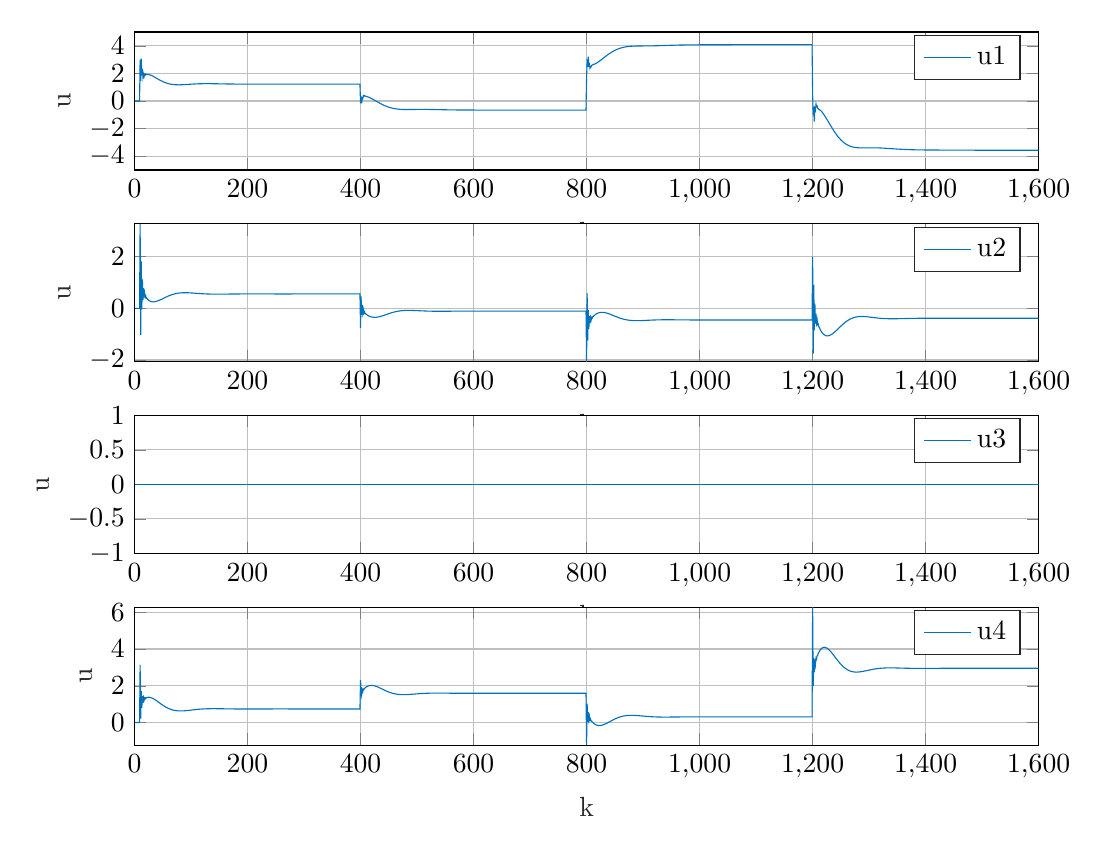
\begin{tikzpicture}

\begin{axis}[%
width=4.521in,
height=0.69in,
at={(0.758in,3.357in)},
scale only axis,
xmin=0,
xmax=1600,
xlabel style={font=\color{white!15!black}},
xlabel={k},
ymin=-5,
ymax=5,
ylabel style={font=\color{white!15!black}},
ylabel={u},
axis background/.style={fill=white},
xmajorgrids,
ymajorgrids,
legend style={legend cell align=left, align=left, draw=white!15!black}
]
\addplot [color=mycolor1]
  table[row sep=crcr]{%
1	0\\
2	0\\
3	0\\
4	0\\
5	0\\
6	0\\
7	0\\
8	0\\
9	0\\
10	2.9925\\
11	1.4423\\
12	3.0753\\
13	1.839\\
14	2.3231\\
15	1.7082\\
16	1.9443\\
17	1.759\\
18	1.9186\\
19	1.8739\\
20	1.9466\\
21	1.9208\\
22	1.9404\\
23	1.9213\\
24	1.9239\\
25	1.9116\\
26	1.9077\\
27	1.8958\\
28	1.8853\\
29	1.8695\\
30	1.8531\\
31	1.8338\\
32	1.8136\\
33	1.7919\\
34	1.7697\\
35	1.7465\\
36	1.723\\
37	1.699\\
38	1.6749\\
39	1.6507\\
40	1.6266\\
41	1.6027\\
42	1.5791\\
43	1.5558\\
44	1.5329\\
45	1.5106\\
46	1.4889\\
47	1.4677\\
48	1.4472\\
49	1.4274\\
50	1.4083\\
51	1.39\\
52	1.3724\\
53	1.3556\\
54	1.3396\\
55	1.3244\\
56	1.31\\
57	1.2964\\
58	1.2836\\
59	1.2717\\
60	1.2605\\
61	1.25\\
62	1.2404\\
63	1.2315\\
64	1.2234\\
65	1.2159\\
66	1.2092\\
67	1.2031\\
68	1.1977\\
69	1.1929\\
70	1.1888\\
71	1.1852\\
72	1.1822\\
73	1.1797\\
74	1.1777\\
75	1.1762\\
76	1.1751\\
77	1.1744\\
78	1.1742\\
79	1.1743\\
80	1.1747\\
81	1.1755\\
82	1.1765\\
83	1.1779\\
84	1.1794\\
85	1.1812\\
86	1.1831\\
87	1.1853\\
88	1.1875\\
89	1.1899\\
90	1.1925\\
91	1.1951\\
92	1.1977\\
93	1.2004\\
94	1.2032\\
95	1.206\\
96	1.2088\\
97	1.2115\\
98	1.2143\\
99	1.217\\
100	1.2197\\
101	1.2223\\
102	1.2249\\
103	1.2274\\
104	1.2298\\
105	1.2322\\
106	1.2344\\
107	1.2366\\
108	1.2387\\
109	1.2406\\
110	1.2425\\
111	1.2442\\
112	1.2458\\
113	1.2474\\
114	1.2488\\
115	1.2501\\
116	1.2513\\
117	1.2524\\
118	1.2533\\
119	1.2542\\
120	1.2549\\
121	1.2556\\
122	1.2562\\
123	1.2566\\
124	1.257\\
125	1.2572\\
126	1.2574\\
127	1.2575\\
128	1.2575\\
129	1.2575\\
130	1.2574\\
131	1.2571\\
132	1.2569\\
133	1.2565\\
134	1.2562\\
135	1.2557\\
136	1.2552\\
137	1.2547\\
138	1.2541\\
139	1.2535\\
140	1.2529\\
141	1.2522\\
142	1.2515\\
143	1.2508\\
144	1.25\\
145	1.2492\\
146	1.2485\\
147	1.2477\\
148	1.2469\\
149	1.2461\\
150	1.2453\\
151	1.2445\\
152	1.2437\\
153	1.2429\\
154	1.2421\\
155	1.2413\\
156	1.2406\\
157	1.2398\\
158	1.2391\\
159	1.2384\\
160	1.2377\\
161	1.237\\
162	1.2363\\
163	1.2357\\
164	1.235\\
165	1.2344\\
166	1.2338\\
167	1.2333\\
168	1.2327\\
169	1.2322\\
170	1.2317\\
171	1.2312\\
172	1.2308\\
173	1.2303\\
174	1.2299\\
175	1.2295\\
176	1.2292\\
177	1.2288\\
178	1.2285\\
179	1.2282\\
180	1.2279\\
181	1.2276\\
182	1.2274\\
183	1.2271\\
184	1.2269\\
185	1.2267\\
186	1.2266\\
187	1.2264\\
188	1.2263\\
189	1.2261\\
190	1.226\\
191	1.2259\\
192	1.2258\\
193	1.2257\\
194	1.2256\\
195	1.2256\\
196	1.2255\\
197	1.2255\\
198	1.2254\\
199	1.2254\\
200	1.2254\\
201	1.2254\\
202	1.2253\\
203	1.2253\\
204	1.2253\\
205	1.2253\\
206	1.2253\\
207	1.2253\\
208	1.2254\\
209	1.2254\\
210	1.2254\\
211	1.2254\\
212	1.2254\\
213	1.2254\\
214	1.2254\\
215	1.2255\\
216	1.2255\\
217	1.2255\\
218	1.2255\\
219	1.2255\\
220	1.2256\\
221	1.2256\\
222	1.2256\\
223	1.2256\\
224	1.2256\\
225	1.2256\\
226	1.2256\\
227	1.2256\\
228	1.2256\\
229	1.2256\\
230	1.2256\\
231	1.2256\\
232	1.2256\\
233	1.2256\\
234	1.2256\\
235	1.2256\\
236	1.2256\\
237	1.2256\\
238	1.2255\\
239	1.2255\\
240	1.2255\\
241	1.2255\\
242	1.2255\\
243	1.2254\\
244	1.2254\\
245	1.2254\\
246	1.2254\\
247	1.2253\\
248	1.2253\\
249	1.2253\\
250	1.2252\\
251	1.2252\\
252	1.2252\\
253	1.2251\\
254	1.2251\\
255	1.2251\\
256	1.225\\
257	1.225\\
258	1.225\\
259	1.2249\\
260	1.2249\\
261	1.2249\\
262	1.2248\\
263	1.2248\\
264	1.2248\\
265	1.2247\\
266	1.2247\\
267	1.2247\\
268	1.2246\\
269	1.2246\\
270	1.2246\\
271	1.2245\\
272	1.2245\\
273	1.2245\\
274	1.2244\\
275	1.2244\\
276	1.2244\\
277	1.2244\\
278	1.2243\\
279	1.2243\\
280	1.2243\\
281	1.2243\\
282	1.2242\\
283	1.2242\\
284	1.2242\\
285	1.2242\\
286	1.2241\\
287	1.2241\\
288	1.2241\\
289	1.2241\\
290	1.2241\\
291	1.2241\\
292	1.224\\
293	1.224\\
294	1.224\\
295	1.224\\
296	1.224\\
297	1.224\\
298	1.224\\
299	1.2239\\
300	1.2239\\
301	1.2239\\
302	1.2239\\
303	1.2239\\
304	1.2239\\
305	1.2239\\
306	1.2239\\
307	1.2239\\
308	1.2239\\
309	1.2238\\
310	1.2238\\
311	1.2238\\
312	1.2238\\
313	1.2238\\
314	1.2238\\
315	1.2238\\
316	1.2238\\
317	1.2238\\
318	1.2238\\
319	1.2238\\
320	1.2238\\
321	1.2238\\
322	1.2238\\
323	1.2238\\
324	1.2238\\
325	1.2238\\
326	1.2238\\
327	1.2238\\
328	1.2238\\
329	1.2237\\
330	1.2237\\
331	1.2237\\
332	1.2237\\
333	1.2237\\
334	1.2237\\
335	1.2237\\
336	1.2237\\
337	1.2237\\
338	1.2237\\
339	1.2237\\
340	1.2237\\
341	1.2237\\
342	1.2237\\
343	1.2237\\
344	1.2237\\
345	1.2237\\
346	1.2237\\
347	1.2237\\
348	1.2237\\
349	1.2237\\
350	1.2237\\
351	1.2237\\
352	1.2237\\
353	1.2237\\
354	1.2237\\
355	1.2237\\
356	1.2237\\
357	1.2237\\
358	1.2237\\
359	1.2237\\
360	1.2237\\
361	1.2237\\
362	1.2237\\
363	1.2237\\
364	1.2237\\
365	1.2237\\
366	1.2237\\
367	1.2237\\
368	1.2236\\
369	1.2236\\
370	1.2236\\
371	1.2236\\
372	1.2236\\
373	1.2236\\
374	1.2236\\
375	1.2236\\
376	1.2236\\
377	1.2236\\
378	1.2236\\
379	1.2236\\
380	1.2236\\
381	1.2236\\
382	1.2236\\
383	1.2236\\
384	1.2236\\
385	1.2236\\
386	1.2236\\
387	1.2236\\
388	1.2236\\
389	1.2236\\
390	1.2236\\
391	1.2236\\
392	1.2236\\
393	1.2236\\
394	1.2236\\
395	1.2236\\
396	1.2236\\
397	1.2236\\
398	1.2236\\
399	1.2236\\
400	-0.17291\\
401	0.33545\\
402	-0.16013\\
403	0.22667\\
404	0.18382\\
405	0.38482\\
406	0.35389\\
407	0.39963\\
408	0.35408\\
409	0.35374\\
410	0.32695\\
411	0.32386\\
412	0.30929\\
413	0.30143\\
414	0.28557\\
415	0.27034\\
416	0.25084\\
417	0.23144\\
418	0.2104\\
419	0.18946\\
420	0.16775\\
421	0.14589\\
422	0.12347\\
423	0.10077\\
424	0.077693\\
425	0.054428\\
426	0.030984\\
427	0.0074766\\
428	-0.016059\\
429	-0.039549\\
430	-0.062952\\
431	-0.08621\\
432	-0.10928\\
433	-0.1321\\
434	-0.15463\\
435	-0.17683\\
436	-0.19864\\
437	-0.22004\\
438	-0.24099\\
439	-0.26145\\
440	-0.28139\\
441	-0.3008\\
442	-0.31963\\
443	-0.33789\\
444	-0.35554\\
445	-0.37257\\
446	-0.38897\\
447	-0.40474\\
448	-0.41986\\
449	-0.43434\\
450	-0.44817\\
451	-0.46135\\
452	-0.47389\\
453	-0.48579\\
454	-0.49706\\
455	-0.50771\\
456	-0.51775\\
457	-0.52718\\
458	-0.53603\\
459	-0.5443\\
460	-0.55202\\
461	-0.55919\\
462	-0.56584\\
463	-0.57199\\
464	-0.57764\\
465	-0.58283\\
466	-0.58756\\
467	-0.59186\\
468	-0.59576\\
469	-0.59926\\
470	-0.60239\\
471	-0.60516\\
472	-0.60761\\
473	-0.60975\\
474	-0.61159\\
475	-0.61316\\
476	-0.61448\\
477	-0.61556\\
478	-0.61642\\
479	-0.61708\\
480	-0.61756\\
481	-0.61788\\
482	-0.61804\\
483	-0.61807\\
484	-0.61798\\
485	-0.61778\\
486	-0.61749\\
487	-0.61712\\
488	-0.61669\\
489	-0.6162\\
490	-0.61566\\
491	-0.6151\\
492	-0.6145\\
493	-0.6139\\
494	-0.61329\\
495	-0.61267\\
496	-0.61207\\
497	-0.61149\\
498	-0.61092\\
499	-0.61038\\
500	-0.60987\\
501	-0.6094\\
502	-0.60897\\
503	-0.60858\\
504	-0.60824\\
505	-0.60795\\
506	-0.60771\\
507	-0.60752\\
508	-0.60738\\
509	-0.6073\\
510	-0.60728\\
511	-0.60731\\
512	-0.60739\\
513	-0.60753\\
514	-0.60772\\
515	-0.60796\\
516	-0.60826\\
517	-0.60861\\
518	-0.609\\
519	-0.60945\\
520	-0.60993\\
521	-0.61047\\
522	-0.61104\\
523	-0.61165\\
524	-0.6123\\
525	-0.61299\\
526	-0.6137\\
527	-0.61445\\
528	-0.61522\\
529	-0.61602\\
530	-0.61685\\
531	-0.61769\\
532	-0.61855\\
533	-0.61942\\
534	-0.62031\\
535	-0.62122\\
536	-0.62213\\
537	-0.62304\\
538	-0.62396\\
539	-0.62489\\
540	-0.62581\\
541	-0.62674\\
542	-0.62766\\
543	-0.62857\\
544	-0.62948\\
545	-0.63038\\
546	-0.63128\\
547	-0.63216\\
548	-0.63303\\
549	-0.63389\\
550	-0.63473\\
551	-0.63556\\
552	-0.63637\\
553	-0.63717\\
554	-0.63795\\
555	-0.63871\\
556	-0.63945\\
557	-0.64018\\
558	-0.64088\\
559	-0.64156\\
560	-0.64223\\
561	-0.64287\\
562	-0.6435\\
563	-0.6441\\
564	-0.64468\\
565	-0.64525\\
566	-0.64579\\
567	-0.64631\\
568	-0.64681\\
569	-0.6473\\
570	-0.64776\\
571	-0.6482\\
572	-0.64863\\
573	-0.64904\\
574	-0.64943\\
575	-0.6498\\
576	-0.65016\\
577	-0.6505\\
578	-0.65082\\
579	-0.65113\\
580	-0.65142\\
581	-0.6517\\
582	-0.65196\\
583	-0.65221\\
584	-0.65245\\
585	-0.65268\\
586	-0.65289\\
587	-0.65309\\
588	-0.65329\\
589	-0.65347\\
590	-0.65364\\
591	-0.65381\\
592	-0.65396\\
593	-0.65411\\
594	-0.65425\\
595	-0.65438\\
596	-0.65451\\
597	-0.65463\\
598	-0.65474\\
599	-0.65485\\
600	-0.65495\\
601	-0.65505\\
602	-0.65515\\
603	-0.65524\\
604	-0.65532\\
605	-0.65541\\
606	-0.65549\\
607	-0.65557\\
608	-0.65564\\
609	-0.65572\\
610	-0.65579\\
611	-0.65586\\
612	-0.65593\\
613	-0.65599\\
614	-0.65606\\
615	-0.65612\\
616	-0.65619\\
617	-0.65625\\
618	-0.65632\\
619	-0.65638\\
620	-0.65644\\
621	-0.6565\\
622	-0.65656\\
623	-0.65662\\
624	-0.65669\\
625	-0.65675\\
626	-0.65681\\
627	-0.65687\\
628	-0.65693\\
629	-0.65699\\
630	-0.65705\\
631	-0.65711\\
632	-0.65717\\
633	-0.65724\\
634	-0.6573\\
635	-0.65736\\
636	-0.65742\\
637	-0.65748\\
638	-0.65754\\
639	-0.6576\\
640	-0.65766\\
641	-0.65772\\
642	-0.65778\\
643	-0.65784\\
644	-0.6579\\
645	-0.65796\\
646	-0.65802\\
647	-0.65808\\
648	-0.65814\\
649	-0.6582\\
650	-0.65825\\
651	-0.65831\\
652	-0.65837\\
653	-0.65842\\
654	-0.65848\\
655	-0.65853\\
656	-0.65859\\
657	-0.65864\\
658	-0.65869\\
659	-0.65874\\
660	-0.65879\\
661	-0.65884\\
662	-0.65889\\
663	-0.65894\\
664	-0.65898\\
665	-0.65903\\
666	-0.65908\\
667	-0.65912\\
668	-0.65916\\
669	-0.65921\\
670	-0.65925\\
671	-0.65929\\
672	-0.65933\\
673	-0.65937\\
674	-0.6594\\
675	-0.65944\\
676	-0.65948\\
677	-0.65951\\
678	-0.65954\\
679	-0.65958\\
680	-0.65961\\
681	-0.65964\\
682	-0.65967\\
683	-0.6597\\
684	-0.65973\\
685	-0.65976\\
686	-0.65978\\
687	-0.65981\\
688	-0.65983\\
689	-0.65986\\
690	-0.65988\\
691	-0.65991\\
692	-0.65993\\
693	-0.65995\\
694	-0.65997\\
695	-0.65999\\
696	-0.66001\\
697	-0.66003\\
698	-0.66005\\
699	-0.66007\\
700	-0.66009\\
701	-0.6601\\
702	-0.66012\\
703	-0.66013\\
704	-0.66015\\
705	-0.66016\\
706	-0.66018\\
707	-0.66019\\
708	-0.66021\\
709	-0.66022\\
710	-0.66023\\
711	-0.66024\\
712	-0.66026\\
713	-0.66027\\
714	-0.66028\\
715	-0.66029\\
716	-0.6603\\
717	-0.66031\\
718	-0.66032\\
719	-0.66033\\
720	-0.66034\\
721	-0.66035\\
722	-0.66036\\
723	-0.66037\\
724	-0.66038\\
725	-0.66039\\
726	-0.6604\\
727	-0.6604\\
728	-0.66041\\
729	-0.66042\\
730	-0.66043\\
731	-0.66043\\
732	-0.66044\\
733	-0.66045\\
734	-0.66046\\
735	-0.66046\\
736	-0.66047\\
737	-0.66048\\
738	-0.66048\\
739	-0.66049\\
740	-0.6605\\
741	-0.6605\\
742	-0.66051\\
743	-0.66052\\
744	-0.66052\\
745	-0.66053\\
746	-0.66053\\
747	-0.66054\\
748	-0.66054\\
749	-0.66055\\
750	-0.66056\\
751	-0.66056\\
752	-0.66057\\
753	-0.66057\\
754	-0.66058\\
755	-0.66058\\
756	-0.66059\\
757	-0.66059\\
758	-0.6606\\
759	-0.6606\\
760	-0.6606\\
761	-0.66061\\
762	-0.66061\\
763	-0.66062\\
764	-0.66062\\
765	-0.66063\\
766	-0.66063\\
767	-0.66063\\
768	-0.66064\\
769	-0.66064\\
770	-0.66065\\
771	-0.66065\\
772	-0.66065\\
773	-0.66066\\
774	-0.66066\\
775	-0.66066\\
776	-0.66067\\
777	-0.66067\\
778	-0.66067\\
779	-0.66068\\
780	-0.66068\\
781	-0.66068\\
782	-0.66069\\
783	-0.66069\\
784	-0.66069\\
785	-0.6607\\
786	-0.6607\\
787	-0.6607\\
788	-0.6607\\
789	-0.66071\\
790	-0.66071\\
791	-0.66071\\
792	-0.66071\\
793	-0.66072\\
794	-0.66072\\
795	-0.66072\\
796	-0.66072\\
797	-0.66073\\
798	-0.66073\\
799	-0.66073\\
800	1.7333\\
801	2.8496\\
802	2.6978\\
803	3.2179\\
804	2.5769\\
805	2.6552\\
806	2.3768\\
807	2.5013\\
808	2.4782\\
809	2.5892\\
810	2.6013\\
811	2.6468\\
812	2.6455\\
813	2.6629\\
814	2.6688\\
815	2.6888\\
816	2.7074\\
817	2.7326\\
818	2.7571\\
819	2.784\\
820	2.8106\\
821	2.8386\\
822	2.867\\
823	2.8966\\
824	2.9268\\
825	2.9578\\
826	2.9891\\
827	3.0209\\
828	3.0528\\
829	3.0848\\
830	3.1168\\
831	3.1488\\
832	3.1806\\
833	3.2122\\
834	3.2435\\
835	3.2744\\
836	3.3049\\
837	3.3349\\
838	3.3645\\
839	3.3934\\
840	3.4218\\
841	3.4495\\
842	3.4766\\
843	3.503\\
844	3.5286\\
845	3.5535\\
846	3.5777\\
847	3.6011\\
848	3.6236\\
849	3.6454\\
850	3.6664\\
851	3.6866\\
852	3.706\\
853	3.7245\\
854	3.7423\\
855	3.7593\\
856	3.7754\\
857	3.7908\\
858	3.8055\\
859	3.8193\\
860	3.8325\\
861	3.8449\\
862	3.8566\\
863	3.8676\\
864	3.878\\
865	3.8877\\
866	3.8968\\
867	3.9053\\
868	3.9132\\
869	3.9205\\
870	3.9274\\
871	3.9337\\
872	3.9395\\
873	3.9448\\
874	3.9497\\
875	3.9542\\
876	3.9583\\
877	3.9621\\
878	3.9655\\
879	3.9685\\
880	3.9713\\
881	3.9737\\
882	3.9759\\
883	3.9779\\
884	3.9797\\
885	3.9812\\
886	3.9825\\
887	3.9837\\
888	3.9848\\
889	3.9857\\
890	3.9864\\
891	3.9871\\
892	3.9877\\
893	3.9882\\
894	3.9886\\
895	3.989\\
896	3.9894\\
897	3.9897\\
898	3.9899\\
899	3.9902\\
900	3.9905\\
901	3.9907\\
902	3.991\\
903	3.9913\\
904	3.9916\\
905	3.9919\\
906	3.9923\\
907	3.9927\\
908	3.9931\\
909	3.9935\\
910	3.994\\
911	3.9946\\
912	3.9952\\
913	3.9958\\
914	3.9965\\
915	3.9972\\
916	3.998\\
917	3.9988\\
918	3.9997\\
919	4.0006\\
920	4.0015\\
921	4.0025\\
922	4.0035\\
923	4.0046\\
924	4.0057\\
925	4.0069\\
926	4.008\\
927	4.0092\\
928	4.0105\\
929	4.0117\\
930	4.013\\
931	4.0143\\
932	4.0156\\
933	4.017\\
934	4.0183\\
935	4.0197\\
936	4.021\\
937	4.0224\\
938	4.0238\\
939	4.0252\\
940	4.0266\\
941	4.0279\\
942	4.0293\\
943	4.0307\\
944	4.032\\
945	4.0334\\
946	4.0347\\
947	4.036\\
948	4.0374\\
949	4.0386\\
950	4.0399\\
951	4.0412\\
952	4.0424\\
953	4.0436\\
954	4.0448\\
955	4.046\\
956	4.0471\\
957	4.0482\\
958	4.0493\\
959	4.0504\\
960	4.0514\\
961	4.0524\\
962	4.0534\\
963	4.0544\\
964	4.0553\\
965	4.0562\\
966	4.0571\\
967	4.0579\\
968	4.0588\\
969	4.0596\\
970	4.0603\\
971	4.0611\\
972	4.0618\\
973	4.0625\\
974	4.0632\\
975	4.0638\\
976	4.0644\\
977	4.065\\
978	4.0656\\
979	4.0661\\
980	4.0667\\
981	4.0672\\
982	4.0676\\
983	4.0681\\
984	4.0686\\
985	4.069\\
986	4.0694\\
987	4.0698\\
988	4.0702\\
989	4.0705\\
990	4.0709\\
991	4.0712\\
992	4.0715\\
993	4.0718\\
994	4.0721\\
995	4.0724\\
996	4.0727\\
997	4.0729\\
998	4.0732\\
999	4.0734\\
1000	4.0736\\
1001	4.0738\\
1002	4.0741\\
1003	4.0743\\
1004	4.0745\\
1005	4.0746\\
1006	4.0748\\
1007	4.075\\
1008	4.0752\\
1009	4.0753\\
1010	4.0755\\
1011	4.0757\\
1012	4.0758\\
1013	4.076\\
1014	4.0761\\
1015	4.0763\\
1016	4.0764\\
1017	4.0765\\
1018	4.0767\\
1019	4.0768\\
1020	4.0769\\
1021	4.0771\\
1022	4.0772\\
1023	4.0773\\
1024	4.0774\\
1025	4.0776\\
1026	4.0777\\
1027	4.0778\\
1028	4.0779\\
1029	4.078\\
1030	4.0781\\
1031	4.0783\\
1032	4.0784\\
1033	4.0785\\
1034	4.0786\\
1035	4.0787\\
1036	4.0788\\
1037	4.0789\\
1038	4.079\\
1039	4.0791\\
1040	4.0792\\
1041	4.0793\\
1042	4.0795\\
1043	4.0796\\
1044	4.0797\\
1045	4.0798\\
1046	4.0799\\
1047	4.08\\
1048	4.0801\\
1049	4.0802\\
1050	4.0802\\
1051	4.0803\\
1052	4.0804\\
1053	4.0805\\
1054	4.0806\\
1055	4.0807\\
1056	4.0808\\
1057	4.0809\\
1058	4.081\\
1059	4.0811\\
1060	4.0811\\
1061	4.0812\\
1062	4.0813\\
1063	4.0814\\
1064	4.0815\\
1065	4.0815\\
1066	4.0816\\
1067	4.0817\\
1068	4.0818\\
1069	4.0818\\
1070	4.0819\\
1071	4.082\\
1072	4.082\\
1073	4.0821\\
1074	4.0822\\
1075	4.0822\\
1076	4.0823\\
1077	4.0823\\
1078	4.0824\\
1079	4.0825\\
1080	4.0825\\
1081	4.0826\\
1082	4.0826\\
1083	4.0827\\
1084	4.0827\\
1085	4.0828\\
1086	4.0828\\
1087	4.0829\\
1088	4.0829\\
1089	4.0829\\
1090	4.083\\
1091	4.083\\
1092	4.0831\\
1093	4.0831\\
1094	4.0831\\
1095	4.0832\\
1096	4.0832\\
1097	4.0832\\
1098	4.0833\\
1099	4.0833\\
1100	4.0833\\
1101	4.0834\\
1102	4.0834\\
1103	4.0834\\
1104	4.0835\\
1105	4.0835\\
1106	4.0835\\
1107	4.0835\\
1108	4.0836\\
1109	4.0836\\
1110	4.0836\\
1111	4.0836\\
1112	4.0837\\
1113	4.0837\\
1114	4.0837\\
1115	4.0837\\
1116	4.0837\\
1117	4.0838\\
1118	4.0838\\
1119	4.0838\\
1120	4.0838\\
1121	4.0838\\
1122	4.0839\\
1123	4.0839\\
1124	4.0839\\
1125	4.0839\\
1126	4.0839\\
1127	4.0839\\
1128	4.0839\\
1129	4.084\\
1130	4.084\\
1131	4.084\\
1132	4.084\\
1133	4.084\\
1134	4.084\\
1135	4.084\\
1136	4.0841\\
1137	4.0841\\
1138	4.0841\\
1139	4.0841\\
1140	4.0841\\
1141	4.0841\\
1142	4.0841\\
1143	4.0841\\
1144	4.0841\\
1145	4.0842\\
1146	4.0842\\
1147	4.0842\\
1148	4.0842\\
1149	4.0842\\
1150	4.0842\\
1151	4.0842\\
1152	4.0842\\
1153	4.0842\\
1154	4.0842\\
1155	4.0843\\
1156	4.0843\\
1157	4.0843\\
1158	4.0843\\
1159	4.0843\\
1160	4.0843\\
1161	4.0843\\
1162	4.0843\\
1163	4.0843\\
1164	4.0843\\
1165	4.0843\\
1166	4.0843\\
1167	4.0843\\
1168	4.0844\\
1169	4.0844\\
1170	4.0844\\
1171	4.0844\\
1172	4.0844\\
1173	4.0844\\
1174	4.0844\\
1175	4.0844\\
1176	4.0844\\
1177	4.0844\\
1178	4.0844\\
1179	4.0844\\
1180	4.0844\\
1181	4.0844\\
1182	4.0844\\
1183	4.0844\\
1184	4.0844\\
1185	4.0845\\
1186	4.0845\\
1187	4.0845\\
1188	4.0845\\
1189	4.0845\\
1190	4.0845\\
1191	4.0845\\
1192	4.0845\\
1193	4.0845\\
1194	4.0845\\
1195	4.0845\\
1196	4.0845\\
1197	4.0845\\
1198	4.0845\\
1199	4.0845\\
1200	0.49352\\
1201	-1.0135\\
1202	-0.77921\\
1203	-1.4955\\
1204	-0.53316\\
1205	-0.63817\\
1206	-0.22358\\
1207	-0.40404\\
1208	-0.36755\\
1209	-0.53007\\
1210	-0.54904\\
1211	-0.62006\\
1212	-0.62517\\
1213	-0.66034\\
1214	-0.68076\\
1215	-0.72366\\
1216	-0.76592\\
1217	-0.81937\\
1218	-0.87271\\
1219	-0.93065\\
1220	-0.98897\\
1221	-1.0501\\
1222	-1.1125\\
1223	-1.1772\\
1224	-1.2431\\
1225	-1.3105\\
1226	-1.3786\\
1227	-1.4475\\
1228	-1.5166\\
1229	-1.5859\\
1230	-1.655\\
1231	-1.7239\\
1232	-1.7924\\
1233	-1.8602\\
1234	-1.9273\\
1235	-1.9935\\
1236	-2.0587\\
1237	-2.1227\\
1238	-2.1855\\
1239	-2.247\\
1240	-2.307\\
1241	-2.3655\\
1242	-2.4224\\
1243	-2.4777\\
1244	-2.5313\\
1245	-2.5832\\
1246	-2.6333\\
1247	-2.6816\\
1248	-2.7281\\
1249	-2.7728\\
1250	-2.8156\\
1251	-2.8566\\
1252	-2.8958\\
1253	-2.9331\\
1254	-2.9687\\
1255	-3.0024\\
1256	-3.0344\\
1257	-3.0647\\
1258	-3.0933\\
1259	-3.1202\\
1260	-3.1455\\
1261	-3.1692\\
1262	-3.1913\\
1263	-3.212\\
1264	-3.2312\\
1265	-3.2491\\
1266	-3.2656\\
1267	-3.2808\\
1268	-3.2948\\
1269	-3.3076\\
1270	-3.3193\\
1271	-3.3299\\
1272	-3.3395\\
1273	-3.3482\\
1274	-3.3559\\
1275	-3.3628\\
1276	-3.369\\
1277	-3.3743\\
1278	-3.379\\
1279	-3.3831\\
1280	-3.3865\\
1281	-3.3894\\
1282	-3.3918\\
1283	-3.3938\\
1284	-3.3953\\
1285	-3.3965\\
1286	-3.3973\\
1287	-3.3979\\
1288	-3.3982\\
1289	-3.3982\\
1290	-3.3981\\
1291	-3.3979\\
1292	-3.3975\\
1293	-3.397\\
1294	-3.3964\\
1295	-3.3958\\
1296	-3.3952\\
1297	-3.3945\\
1298	-3.3939\\
1299	-3.3933\\
1300	-3.3927\\
1301	-3.3922\\
1302	-3.3918\\
1303	-3.3914\\
1304	-3.3912\\
1305	-3.391\\
1306	-3.391\\
1307	-3.3911\\
1308	-3.3913\\
1309	-3.3916\\
1310	-3.392\\
1311	-3.3926\\
1312	-3.3933\\
1313	-3.3942\\
1314	-3.3952\\
1315	-3.3963\\
1316	-3.3975\\
1317	-3.3989\\
1318	-3.4004\\
1319	-3.402\\
1320	-3.4037\\
1321	-3.4055\\
1322	-3.4075\\
1323	-3.4095\\
1324	-3.4117\\
1325	-3.4139\\
1326	-3.4162\\
1327	-3.4186\\
1328	-3.421\\
1329	-3.4236\\
1330	-3.4262\\
1331	-3.4288\\
1332	-3.4315\\
1333	-3.4342\\
1334	-3.437\\
1335	-3.4398\\
1336	-3.4426\\
1337	-3.4454\\
1338	-3.4483\\
1339	-3.4511\\
1340	-3.4539\\
1341	-3.4568\\
1342	-3.4596\\
1343	-3.4624\\
1344	-3.4652\\
1345	-3.468\\
1346	-3.4708\\
1347	-3.4735\\
1348	-3.4762\\
1349	-3.4788\\
1350	-3.4815\\
1351	-3.484\\
1352	-3.4865\\
1353	-3.489\\
1354	-3.4914\\
1355	-3.4938\\
1356	-3.4961\\
1357	-3.4984\\
1358	-3.5006\\
1359	-3.5027\\
1360	-3.5048\\
1361	-3.5069\\
1362	-3.5088\\
1363	-3.5107\\
1364	-3.5126\\
1365	-3.5144\\
1366	-3.5161\\
1367	-3.5178\\
1368	-3.5194\\
1369	-3.521\\
1370	-3.5225\\
1371	-3.5239\\
1372	-3.5253\\
1373	-3.5266\\
1374	-3.5279\\
1375	-3.5292\\
1376	-3.5303\\
1377	-3.5315\\
1378	-3.5325\\
1379	-3.5336\\
1380	-3.5346\\
1381	-3.5355\\
1382	-3.5364\\
1383	-3.5373\\
1384	-3.5381\\
1385	-3.5389\\
1386	-3.5396\\
1387	-3.5403\\
1388	-3.541\\
1389	-3.5417\\
1390	-3.5423\\
1391	-3.5429\\
1392	-3.5434\\
1393	-3.544\\
1394	-3.5445\\
1395	-3.545\\
1396	-3.5454\\
1397	-3.5459\\
1398	-3.5463\\
1399	-3.5467\\
1400	-3.5471\\
1401	-3.5475\\
1402	-3.5478\\
1403	-3.5482\\
1404	-3.5485\\
1405	-3.5488\\
1406	-3.5491\\
1407	-3.5494\\
1408	-3.5497\\
1409	-3.55\\
1410	-3.5503\\
1411	-3.5505\\
1412	-3.5508\\
1413	-3.5511\\
1414	-3.5513\\
1415	-3.5516\\
1416	-3.5518\\
1417	-3.552\\
1418	-3.5523\\
1419	-3.5525\\
1420	-3.5527\\
1421	-3.5529\\
1422	-3.5532\\
1423	-3.5534\\
1424	-3.5536\\
1425	-3.5538\\
1426	-3.554\\
1427	-3.5543\\
1428	-3.5545\\
1429	-3.5547\\
1430	-3.5549\\
1431	-3.5551\\
1432	-3.5553\\
1433	-3.5555\\
1434	-3.5557\\
1435	-3.5559\\
1436	-3.5562\\
1437	-3.5564\\
1438	-3.5566\\
1439	-3.5568\\
1440	-3.557\\
1441	-3.5572\\
1442	-3.5574\\
1443	-3.5576\\
1444	-3.5578\\
1445	-3.558\\
1446	-3.5582\\
1447	-3.5583\\
1448	-3.5585\\
1449	-3.5587\\
1450	-3.5589\\
1451	-3.5591\\
1452	-3.5593\\
1453	-3.5595\\
1454	-3.5596\\
1455	-3.5598\\
1456	-3.56\\
1457	-3.5602\\
1458	-3.5603\\
1459	-3.5605\\
1460	-3.5607\\
1461	-3.5608\\
1462	-3.561\\
1463	-3.5611\\
1464	-3.5613\\
1465	-3.5614\\
1466	-3.5616\\
1467	-3.5617\\
1468	-3.5619\\
1469	-3.562\\
1470	-3.5621\\
1471	-3.5623\\
1472	-3.5624\\
1473	-3.5625\\
1474	-3.5626\\
1475	-3.5628\\
1476	-3.5629\\
1477	-3.563\\
1478	-3.5631\\
1479	-3.5632\\
1480	-3.5633\\
1481	-3.5634\\
1482	-3.5635\\
1483	-3.5636\\
1484	-3.5637\\
1485	-3.5638\\
1486	-3.5639\\
1487	-3.564\\
1488	-3.5641\\
1489	-3.5641\\
1490	-3.5642\\
1491	-3.5643\\
1492	-3.5644\\
1493	-3.5644\\
1494	-3.5645\\
1495	-3.5646\\
1496	-3.5646\\
1497	-3.5647\\
1498	-3.5648\\
1499	-3.5648\\
1500	-3.5649\\
1501	-3.5649\\
1502	-3.565\\
1503	-3.5651\\
1504	-3.5651\\
1505	-3.5652\\
1506	-3.5652\\
1507	-3.5653\\
1508	-3.5653\\
1509	-3.5654\\
1510	-3.5654\\
1511	-3.5654\\
1512	-3.5655\\
1513	-3.5655\\
1514	-3.5656\\
1515	-3.5656\\
1516	-3.5656\\
1517	-3.5657\\
1518	-3.5657\\
1519	-3.5657\\
1520	-3.5658\\
1521	-3.5658\\
1522	-3.5658\\
1523	-3.5659\\
1524	-3.5659\\
1525	-3.5659\\
1526	-3.566\\
1527	-3.566\\
1528	-3.566\\
1529	-3.566\\
1530	-3.5661\\
1531	-3.5661\\
1532	-3.5661\\
1533	-3.5661\\
1534	-3.5662\\
1535	-3.5662\\
1536	-3.5662\\
1537	-3.5662\\
1538	-3.5663\\
1539	-3.5663\\
1540	-3.5663\\
1541	-3.5663\\
1542	-3.5663\\
1543	-3.5664\\
1544	-3.5664\\
1545	-3.5664\\
1546	-3.5664\\
1547	-3.5664\\
1548	-3.5665\\
1549	-3.5665\\
1550	-3.5665\\
1551	-3.5665\\
1552	-3.5665\\
1553	-3.5666\\
1554	-3.5666\\
1555	-3.5666\\
1556	-3.5666\\
1557	-3.5666\\
1558	-3.5666\\
1559	-3.5667\\
1560	-3.5667\\
1561	-3.5667\\
1562	-3.5667\\
1563	-3.5667\\
1564	-3.5667\\
1565	-3.5667\\
1566	-3.5668\\
1567	-3.5668\\
1568	-3.5668\\
1569	-3.5668\\
1570	-3.5668\\
1571	-3.5668\\
1572	-3.5668\\
1573	-3.5668\\
1574	-3.5669\\
1575	-3.5669\\
1576	-3.5669\\
1577	-3.5669\\
1578	-3.5669\\
1579	-3.5669\\
1580	-3.5669\\
1581	-3.5669\\
1582	-3.5669\\
1583	-3.567\\
1584	-3.567\\
1585	-3.567\\
1586	-3.567\\
1587	-3.567\\
1588	-3.567\\
1589	-3.567\\
1590	-3.567\\
1591	-3.567\\
1592	-3.567\\
1593	-3.567\\
1594	-3.567\\
1595	-3.5671\\
1596	-3.5671\\
1597	-3.5671\\
1598	-3.5671\\
1599	-3.5671\\
1600	-3.5671\\
};
\addlegendentry{u1}

\end{axis}

\begin{axis}[%
width=4.521in,
height=0.69in,
at={(0.758in,2.398in)},
scale only axis,
xmin=0,
xmax=1600,
xlabel style={font=\color{white!15!black}},
xlabel={k},
ymin=-2.0717,
ymax=3.2744,
ylabel style={font=\color{white!15!black}},
ylabel={u},
axis background/.style={fill=white},
xmajorgrids,
ymajorgrids,
legend style={legend cell align=left, align=left, draw=white!15!black}
]
\addplot [color=mycolor1]
  table[row sep=crcr]{%
1	0\\
2	0\\
3	0\\
4	0\\
5	0\\
6	0\\
7	0\\
8	0\\
9	0\\
10	3.2744\\
11	-1.0328\\
12	1.819\\
13	-0.038181\\
14	1.1191\\
15	0.32637\\
16	0.78167\\
17	0.42867\\
18	0.59434\\
19	0.42675\\
20	0.47654\\
21	0.39045\\
22	0.39672\\
23	0.3487\\
24	0.34086\\
25	0.31223\\
26	0.30189\\
27	0.28442\\
28	0.2759\\
29	0.26568\\
30	0.26029\\
31	0.25522\\
32	0.25306\\
33	0.25186\\
34	0.2526\\
35	0.2544\\
36	0.25761\\
37	0.26178\\
38	0.26702\\
39	0.27308\\
40	0.27995\\
41	0.2875\\
42	0.29566\\
43	0.30435\\
44	0.3135\\
45	0.32304\\
46	0.33291\\
47	0.34304\\
48	0.35337\\
49	0.36386\\
50	0.37445\\
51	0.38509\\
52	0.39574\\
53	0.40635\\
54	0.4169\\
55	0.42733\\
56	0.43761\\
57	0.44772\\
58	0.45762\\
59	0.4673\\
60	0.47671\\
61	0.48586\\
62	0.4947\\
63	0.50324\\
64	0.51145\\
65	0.51932\\
66	0.52685\\
67	0.53402\\
68	0.54084\\
69	0.54728\\
70	0.55336\\
71	0.55908\\
72	0.56442\\
73	0.5694\\
74	0.57402\\
75	0.57828\\
76	0.58219\\
77	0.58575\\
78	0.58898\\
79	0.59188\\
80	0.59446\\
81	0.59673\\
82	0.5987\\
83	0.60038\\
84	0.60179\\
85	0.60293\\
86	0.60382\\
87	0.60447\\
88	0.60489\\
89	0.6051\\
90	0.60511\\
91	0.60493\\
92	0.60457\\
93	0.60404\\
94	0.60337\\
95	0.60255\\
96	0.60161\\
97	0.60055\\
98	0.59938\\
99	0.59813\\
100	0.59679\\
101	0.59537\\
102	0.5939\\
103	0.59237\\
104	0.5908\\
105	0.5892\\
106	0.58757\\
107	0.58592\\
108	0.58426\\
109	0.5826\\
110	0.58094\\
111	0.5793\\
112	0.57766\\
113	0.57605\\
114	0.57447\\
115	0.57291\\
116	0.57139\\
117	0.56991\\
118	0.56847\\
119	0.56708\\
120	0.56573\\
121	0.56444\\
122	0.56319\\
123	0.562\\
124	0.56087\\
125	0.55979\\
126	0.55876\\
127	0.5578\\
128	0.55689\\
129	0.55604\\
130	0.55524\\
131	0.5545\\
132	0.55382\\
133	0.55319\\
134	0.55262\\
135	0.5521\\
136	0.55163\\
137	0.55121\\
138	0.55084\\
139	0.55052\\
140	0.55025\\
141	0.55001\\
142	0.54982\\
143	0.54967\\
144	0.54956\\
145	0.54949\\
146	0.54945\\
147	0.54944\\
148	0.54946\\
149	0.54951\\
150	0.54959\\
151	0.54969\\
152	0.54981\\
153	0.54996\\
154	0.55012\\
155	0.5503\\
156	0.5505\\
157	0.55071\\
158	0.55093\\
159	0.55116\\
160	0.55141\\
161	0.55165\\
162	0.55191\\
163	0.55217\\
164	0.55243\\
165	0.5527\\
166	0.55296\\
167	0.55323\\
168	0.5535\\
169	0.55376\\
170	0.55402\\
171	0.55428\\
172	0.55453\\
173	0.55478\\
174	0.55502\\
175	0.55526\\
176	0.55548\\
177	0.55571\\
178	0.55592\\
179	0.55613\\
180	0.55632\\
181	0.55651\\
182	0.55669\\
183	0.55686\\
184	0.55703\\
185	0.55718\\
186	0.55733\\
187	0.55746\\
188	0.55759\\
189	0.55771\\
190	0.55782\\
191	0.55792\\
192	0.55801\\
193	0.55809\\
194	0.55817\\
195	0.55824\\
196	0.5583\\
197	0.55835\\
198	0.5584\\
199	0.55844\\
200	0.55847\\
201	0.5585\\
202	0.55852\\
203	0.55854\\
204	0.55855\\
205	0.55855\\
206	0.55855\\
207	0.55855\\
208	0.55854\\
209	0.55853\\
210	0.55851\\
211	0.55849\\
212	0.55847\\
213	0.55845\\
214	0.55842\\
215	0.55839\\
216	0.55836\\
217	0.55833\\
218	0.5583\\
219	0.55826\\
220	0.55823\\
221	0.55819\\
222	0.55815\\
223	0.55812\\
224	0.55808\\
225	0.55804\\
226	0.558\\
227	0.55797\\
228	0.55793\\
229	0.5579\\
230	0.55786\\
231	0.55783\\
232	0.55779\\
233	0.55776\\
234	0.55773\\
235	0.5577\\
236	0.55767\\
237	0.55764\\
238	0.55761\\
239	0.55758\\
240	0.55756\\
241	0.55754\\
242	0.55751\\
243	0.55749\\
244	0.55747\\
245	0.55746\\
246	0.55744\\
247	0.55742\\
248	0.55741\\
249	0.5574\\
250	0.55739\\
251	0.55738\\
252	0.55737\\
253	0.55736\\
254	0.55735\\
255	0.55735\\
256	0.55734\\
257	0.55734\\
258	0.55733\\
259	0.55733\\
260	0.55733\\
261	0.55733\\
262	0.55733\\
263	0.55733\\
264	0.55733\\
265	0.55734\\
266	0.55734\\
267	0.55734\\
268	0.55735\\
269	0.55735\\
270	0.55736\\
271	0.55736\\
272	0.55737\\
273	0.55737\\
274	0.55738\\
275	0.55739\\
276	0.55739\\
277	0.5574\\
278	0.55741\\
279	0.55741\\
280	0.55742\\
281	0.55743\\
282	0.55743\\
283	0.55744\\
284	0.55745\\
285	0.55745\\
286	0.55746\\
287	0.55747\\
288	0.55747\\
289	0.55748\\
290	0.55749\\
291	0.55749\\
292	0.5575\\
293	0.5575\\
294	0.55751\\
295	0.55751\\
296	0.55752\\
297	0.55752\\
298	0.55753\\
299	0.55753\\
300	0.55754\\
301	0.55754\\
302	0.55754\\
303	0.55755\\
304	0.55755\\
305	0.55755\\
306	0.55756\\
307	0.55756\\
308	0.55756\\
309	0.55756\\
310	0.55757\\
311	0.55757\\
312	0.55757\\
313	0.55757\\
314	0.55757\\
315	0.55757\\
316	0.55757\\
317	0.55757\\
318	0.55758\\
319	0.55758\\
320	0.55758\\
321	0.55758\\
322	0.55758\\
323	0.55758\\
324	0.55758\\
325	0.55758\\
326	0.55758\\
327	0.55758\\
328	0.55758\\
329	0.55758\\
330	0.55757\\
331	0.55757\\
332	0.55757\\
333	0.55757\\
334	0.55757\\
335	0.55757\\
336	0.55757\\
337	0.55757\\
338	0.55757\\
339	0.55757\\
340	0.55757\\
341	0.55757\\
342	0.55757\\
343	0.55757\\
344	0.55757\\
345	0.55756\\
346	0.55756\\
347	0.55756\\
348	0.55756\\
349	0.55756\\
350	0.55756\\
351	0.55756\\
352	0.55756\\
353	0.55756\\
354	0.55756\\
355	0.55756\\
356	0.55756\\
357	0.55756\\
358	0.55756\\
359	0.55756\\
360	0.55756\\
361	0.55756\\
362	0.55756\\
363	0.55756\\
364	0.55756\\
365	0.55756\\
366	0.55756\\
367	0.55755\\
368	0.55755\\
369	0.55755\\
370	0.55755\\
371	0.55755\\
372	0.55755\\
373	0.55755\\
374	0.55755\\
375	0.55755\\
376	0.55755\\
377	0.55755\\
378	0.55755\\
379	0.55755\\
380	0.55756\\
381	0.55756\\
382	0.55756\\
383	0.55756\\
384	0.55756\\
385	0.55756\\
386	0.55756\\
387	0.55756\\
388	0.55756\\
389	0.55756\\
390	0.55756\\
391	0.55756\\
392	0.55756\\
393	0.55756\\
394	0.55756\\
395	0.55756\\
396	0.55756\\
397	0.55756\\
398	0.55756\\
399	0.55756\\
400	-0.75222\\
401	0.45828\\
402	-0.25054\\
403	0.13193\\
404	-0.18284\\
405	-0.040654\\
406	-0.1855\\
407	-0.1387\\
408	-0.2095\\
409	-0.19975\\
410	-0.23796\\
411	-0.24203\\
412	-0.26529\\
413	-0.27368\\
414	-0.28932\\
415	-0.29813\\
416	-0.30928\\
417	-0.31696\\
418	-0.32501\\
419	-0.33103\\
420	-0.33661\\
421	-0.34079\\
422	-0.34423\\
423	-0.34656\\
424	-0.34808\\
425	-0.34865\\
426	-0.34843\\
427	-0.34738\\
428	-0.34558\\
429	-0.34307\\
430	-0.3399\\
431	-0.33611\\
432	-0.33175\\
433	-0.32687\\
434	-0.32151\\
435	-0.31572\\
436	-0.30956\\
437	-0.30305\\
438	-0.29626\\
439	-0.28921\\
440	-0.28196\\
441	-0.27453\\
442	-0.26698\\
443	-0.25932\\
444	-0.25161\\
445	-0.24387\\
446	-0.23613\\
447	-0.22841\\
448	-0.22076\\
449	-0.21319\\
450	-0.20572\\
451	-0.19838\\
452	-0.19118\\
453	-0.18414\\
454	-0.17729\\
455	-0.17063\\
456	-0.16417\\
457	-0.15794\\
458	-0.15192\\
459	-0.14615\\
460	-0.14062\\
461	-0.13533\\
462	-0.1303\\
463	-0.12552\\
464	-0.12099\\
465	-0.11673\\
466	-0.11272\\
467	-0.10897\\
468	-0.10547\\
469	-0.10222\\
470	-0.099217\\
471	-0.096458\\
472	-0.093935\\
473	-0.091645\\
474	-0.089579\\
475	-0.087733\\
476	-0.086098\\
477	-0.084668\\
478	-0.083434\\
479	-0.082388\\
480	-0.081522\\
481	-0.080829\\
482	-0.080298\\
483	-0.079923\\
484	-0.079693\\
485	-0.0796\\
486	-0.079636\\
487	-0.079792\\
488	-0.08006\\
489	-0.080431\\
490	-0.080896\\
491	-0.081448\\
492	-0.082079\\
493	-0.082781\\
494	-0.083546\\
495	-0.084368\\
496	-0.085239\\
497	-0.086152\\
498	-0.087101\\
499	-0.08808\\
500	-0.089082\\
501	-0.090103\\
502	-0.091136\\
503	-0.092177\\
504	-0.093221\\
505	-0.094263\\
506	-0.095299\\
507	-0.096326\\
508	-0.097339\\
509	-0.098335\\
510	-0.099312\\
511	-0.10027\\
512	-0.1012\\
513	-0.1021\\
514	-0.10297\\
515	-0.10381\\
516	-0.10462\\
517	-0.1054\\
518	-0.10614\\
519	-0.10684\\
520	-0.10751\\
521	-0.10814\\
522	-0.10874\\
523	-0.10929\\
524	-0.10981\\
525	-0.1103\\
526	-0.11074\\
527	-0.11115\\
528	-0.11153\\
529	-0.11186\\
530	-0.11217\\
531	-0.11244\\
532	-0.11268\\
533	-0.11288\\
534	-0.11306\\
535	-0.1132\\
536	-0.11332\\
537	-0.11341\\
538	-0.11348\\
539	-0.11352\\
540	-0.11354\\
541	-0.11353\\
542	-0.11351\\
543	-0.11346\\
544	-0.1134\\
545	-0.11332\\
546	-0.11322\\
547	-0.11311\\
548	-0.11299\\
549	-0.11285\\
550	-0.11271\\
551	-0.11255\\
552	-0.11239\\
553	-0.11222\\
554	-0.11204\\
555	-0.11186\\
556	-0.11168\\
557	-0.11149\\
558	-0.11129\\
559	-0.1111\\
560	-0.11091\\
561	-0.11071\\
562	-0.11052\\
563	-0.11033\\
564	-0.11013\\
565	-0.10995\\
566	-0.10976\\
567	-0.10958\\
568	-0.1094\\
569	-0.10923\\
570	-0.10906\\
571	-0.10889\\
572	-0.10873\\
573	-0.10858\\
574	-0.10843\\
575	-0.10829\\
576	-0.10816\\
577	-0.10803\\
578	-0.1079\\
579	-0.10778\\
580	-0.10767\\
581	-0.10757\\
582	-0.10747\\
583	-0.10738\\
584	-0.10729\\
585	-0.10721\\
586	-0.10714\\
587	-0.10707\\
588	-0.107\\
589	-0.10695\\
590	-0.1069\\
591	-0.10685\\
592	-0.10681\\
593	-0.10677\\
594	-0.10674\\
595	-0.10671\\
596	-0.10669\\
597	-0.10667\\
598	-0.10665\\
599	-0.10664\\
600	-0.10663\\
601	-0.10663\\
602	-0.10662\\
603	-0.10662\\
604	-0.10663\\
605	-0.10663\\
606	-0.10664\\
607	-0.10665\\
608	-0.10666\\
609	-0.10668\\
610	-0.10669\\
611	-0.10671\\
612	-0.10672\\
613	-0.10674\\
614	-0.10676\\
615	-0.10678\\
616	-0.1068\\
617	-0.10682\\
618	-0.10684\\
619	-0.10687\\
620	-0.10689\\
621	-0.10691\\
622	-0.10693\\
623	-0.10695\\
624	-0.10697\\
625	-0.10699\\
626	-0.10701\\
627	-0.10703\\
628	-0.10705\\
629	-0.10707\\
630	-0.10708\\
631	-0.1071\\
632	-0.10712\\
633	-0.10713\\
634	-0.10715\\
635	-0.10716\\
636	-0.10717\\
637	-0.10719\\
638	-0.1072\\
639	-0.10721\\
640	-0.10722\\
641	-0.10722\\
642	-0.10723\\
643	-0.10724\\
644	-0.10725\\
645	-0.10725\\
646	-0.10726\\
647	-0.10726\\
648	-0.10726\\
649	-0.10727\\
650	-0.10727\\
651	-0.10727\\
652	-0.10727\\
653	-0.10727\\
654	-0.10727\\
655	-0.10727\\
656	-0.10727\\
657	-0.10726\\
658	-0.10726\\
659	-0.10726\\
660	-0.10726\\
661	-0.10725\\
662	-0.10725\\
663	-0.10724\\
664	-0.10724\\
665	-0.10723\\
666	-0.10723\\
667	-0.10722\\
668	-0.10722\\
669	-0.10721\\
670	-0.10721\\
671	-0.1072\\
672	-0.1072\\
673	-0.10719\\
674	-0.10719\\
675	-0.10718\\
676	-0.10717\\
677	-0.10717\\
678	-0.10716\\
679	-0.10716\\
680	-0.10715\\
681	-0.10715\\
682	-0.10714\\
683	-0.10714\\
684	-0.10713\\
685	-0.10713\\
686	-0.10712\\
687	-0.10712\\
688	-0.10711\\
689	-0.10711\\
690	-0.1071\\
691	-0.1071\\
692	-0.1071\\
693	-0.10709\\
694	-0.10709\\
695	-0.10709\\
696	-0.10708\\
697	-0.10708\\
698	-0.10708\\
699	-0.10707\\
700	-0.10707\\
701	-0.10707\\
702	-0.10707\\
703	-0.10706\\
704	-0.10706\\
705	-0.10706\\
706	-0.10706\\
707	-0.10706\\
708	-0.10706\\
709	-0.10705\\
710	-0.10705\\
711	-0.10705\\
712	-0.10705\\
713	-0.10705\\
714	-0.10705\\
715	-0.10705\\
716	-0.10705\\
717	-0.10705\\
718	-0.10705\\
719	-0.10705\\
720	-0.10705\\
721	-0.10705\\
722	-0.10705\\
723	-0.10705\\
724	-0.10705\\
725	-0.10705\\
726	-0.10705\\
727	-0.10705\\
728	-0.10705\\
729	-0.10705\\
730	-0.10705\\
731	-0.10705\\
732	-0.10705\\
733	-0.10705\\
734	-0.10705\\
735	-0.10705\\
736	-0.10705\\
737	-0.10705\\
738	-0.10705\\
739	-0.10705\\
740	-0.10705\\
741	-0.10705\\
742	-0.10705\\
743	-0.10705\\
744	-0.10705\\
745	-0.10705\\
746	-0.10705\\
747	-0.10705\\
748	-0.10705\\
749	-0.10705\\
750	-0.10705\\
751	-0.10705\\
752	-0.10705\\
753	-0.10705\\
754	-0.10705\\
755	-0.10705\\
756	-0.10705\\
757	-0.10705\\
758	-0.10705\\
759	-0.10705\\
760	-0.10705\\
761	-0.10705\\
762	-0.10705\\
763	-0.10705\\
764	-0.10705\\
765	-0.10705\\
766	-0.10705\\
767	-0.10705\\
768	-0.10705\\
769	-0.10705\\
770	-0.10705\\
771	-0.10705\\
772	-0.10705\\
773	-0.10705\\
774	-0.10705\\
775	-0.10705\\
776	-0.10705\\
777	-0.10705\\
778	-0.10705\\
779	-0.10705\\
780	-0.10705\\
781	-0.10705\\
782	-0.10705\\
783	-0.10705\\
784	-0.10705\\
785	-0.10705\\
786	-0.10705\\
787	-0.10705\\
788	-0.10705\\
789	-0.10705\\
790	-0.10705\\
791	-0.10705\\
792	-0.10705\\
793	-0.10704\\
794	-0.10704\\
795	-0.10704\\
796	-0.10704\\
797	-0.10704\\
798	-0.10704\\
799	-0.10704\\
800	-2.0717\\
801	0.5871\\
802	-1.2412\\
803	-0.074491\\
804	-0.80399\\
805	-0.30168\\
806	-0.58416\\
807	-0.35851\\
808	-0.45953\\
809	-0.35088\\
810	-0.37842\\
811	-0.31978\\
812	-0.31855\\
813	-0.28264\\
814	-0.27169\\
815	-0.24753\\
816	-0.23483\\
817	-0.21771\\
818	-0.20632\\
819	-0.19401\\
820	-0.18493\\
821	-0.17629\\
822	-0.16976\\
823	-0.16414\\
824	-0.16009\\
825	-0.15706\\
826	-0.15529\\
827	-0.15451\\
828	-0.15478\\
829	-0.15597\\
830	-0.15805\\
831	-0.16095\\
832	-0.16461\\
833	-0.16897\\
834	-0.17399\\
835	-0.17961\\
836	-0.18577\\
837	-0.19242\\
838	-0.19951\\
839	-0.207\\
840	-0.21483\\
841	-0.22296\\
842	-0.23135\\
843	-0.23994\\
844	-0.2487\\
845	-0.25759\\
846	-0.26657\\
847	-0.27561\\
848	-0.28466\\
849	-0.29369\\
850	-0.30269\\
851	-0.3116\\
852	-0.32042\\
853	-0.32911\\
854	-0.33765\\
855	-0.34602\\
856	-0.35419\\
857	-0.36216\\
858	-0.36991\\
859	-0.37742\\
860	-0.38468\\
861	-0.39168\\
862	-0.3984\\
863	-0.40486\\
864	-0.41103\\
865	-0.41691\\
866	-0.4225\\
867	-0.4278\\
868	-0.4328\\
869	-0.43751\\
870	-0.44193\\
871	-0.44606\\
872	-0.44991\\
873	-0.45347\\
874	-0.45676\\
875	-0.45977\\
876	-0.46253\\
877	-0.46502\\
878	-0.46727\\
879	-0.46927\\
880	-0.47104\\
881	-0.47258\\
882	-0.47391\\
883	-0.47503\\
884	-0.47596\\
885	-0.47669\\
886	-0.47725\\
887	-0.47765\\
888	-0.47788\\
889	-0.47796\\
890	-0.47791\\
891	-0.47773\\
892	-0.47743\\
893	-0.47702\\
894	-0.4765\\
895	-0.4759\\
896	-0.47521\\
897	-0.47445\\
898	-0.47362\\
899	-0.47273\\
900	-0.47179\\
901	-0.47081\\
902	-0.46979\\
903	-0.46874\\
904	-0.46767\\
905	-0.46658\\
906	-0.46548\\
907	-0.46437\\
908	-0.46326\\
909	-0.46216\\
910	-0.46107\\
911	-0.45998\\
912	-0.45892\\
913	-0.45787\\
914	-0.45685\\
915	-0.45585\\
916	-0.45489\\
917	-0.45395\\
918	-0.45305\\
919	-0.45218\\
920	-0.45134\\
921	-0.45055\\
922	-0.44979\\
923	-0.44907\\
924	-0.4484\\
925	-0.44776\\
926	-0.44716\\
927	-0.44661\\
928	-0.44609\\
929	-0.44562\\
930	-0.44518\\
931	-0.44479\\
932	-0.44443\\
933	-0.44411\\
934	-0.44383\\
935	-0.44358\\
936	-0.44337\\
937	-0.44319\\
938	-0.44305\\
939	-0.44294\\
940	-0.44285\\
941	-0.44279\\
942	-0.44277\\
943	-0.44276\\
944	-0.44278\\
945	-0.44283\\
946	-0.44289\\
947	-0.44298\\
948	-0.44308\\
949	-0.4432\\
950	-0.44334\\
951	-0.44349\\
952	-0.44366\\
953	-0.44383\\
954	-0.44402\\
955	-0.44422\\
956	-0.44442\\
957	-0.44463\\
958	-0.44485\\
959	-0.44507\\
960	-0.44529\\
961	-0.44552\\
962	-0.44575\\
963	-0.44598\\
964	-0.44621\\
965	-0.44643\\
966	-0.44666\\
967	-0.44689\\
968	-0.44711\\
969	-0.44733\\
970	-0.44754\\
971	-0.44775\\
972	-0.44796\\
973	-0.44816\\
974	-0.44835\\
975	-0.44854\\
976	-0.44872\\
977	-0.44889\\
978	-0.44906\\
979	-0.44922\\
980	-0.44938\\
981	-0.44953\\
982	-0.44967\\
983	-0.4498\\
984	-0.44993\\
985	-0.45005\\
986	-0.45016\\
987	-0.45026\\
988	-0.45036\\
989	-0.45045\\
990	-0.45054\\
991	-0.45061\\
992	-0.45069\\
993	-0.45075\\
994	-0.45081\\
995	-0.45086\\
996	-0.45091\\
997	-0.45095\\
998	-0.45099\\
999	-0.45102\\
1000	-0.45105\\
1001	-0.45108\\
1002	-0.4511\\
1003	-0.45111\\
1004	-0.45112\\
1005	-0.45113\\
1006	-0.45113\\
1007	-0.45114\\
1008	-0.45113\\
1009	-0.45113\\
1010	-0.45112\\
1011	-0.45112\\
1012	-0.4511\\
1013	-0.45109\\
1014	-0.45108\\
1015	-0.45106\\
1016	-0.45105\\
1017	-0.45103\\
1018	-0.45101\\
1019	-0.45099\\
1020	-0.45097\\
1021	-0.45095\\
1022	-0.45093\\
1023	-0.45091\\
1024	-0.45089\\
1025	-0.45087\\
1026	-0.45085\\
1027	-0.45083\\
1028	-0.45081\\
1029	-0.45079\\
1030	-0.45077\\
1031	-0.45075\\
1032	-0.45073\\
1033	-0.45072\\
1034	-0.4507\\
1035	-0.45068\\
1036	-0.45067\\
1037	-0.45065\\
1038	-0.45064\\
1039	-0.45063\\
1040	-0.45062\\
1041	-0.45061\\
1042	-0.4506\\
1043	-0.45059\\
1044	-0.45058\\
1045	-0.45057\\
1046	-0.45057\\
1047	-0.45056\\
1048	-0.45056\\
1049	-0.45055\\
1050	-0.45055\\
1051	-0.45055\\
1052	-0.45055\\
1053	-0.45055\\
1054	-0.45055\\
1055	-0.45055\\
1056	-0.45055\\
1057	-0.45055\\
1058	-0.45055\\
1059	-0.45056\\
1060	-0.45056\\
1061	-0.45056\\
1062	-0.45057\\
1063	-0.45057\\
1064	-0.45058\\
1065	-0.45058\\
1066	-0.45059\\
1067	-0.45059\\
1068	-0.4506\\
1069	-0.45061\\
1070	-0.45061\\
1071	-0.45062\\
1072	-0.45063\\
1073	-0.45063\\
1074	-0.45064\\
1075	-0.45065\\
1076	-0.45066\\
1077	-0.45066\\
1078	-0.45067\\
1079	-0.45068\\
1080	-0.45069\\
1081	-0.45069\\
1082	-0.4507\\
1083	-0.45071\\
1084	-0.45071\\
1085	-0.45072\\
1086	-0.45073\\
1087	-0.45073\\
1088	-0.45074\\
1089	-0.45074\\
1090	-0.45075\\
1091	-0.45076\\
1092	-0.45076\\
1093	-0.45077\\
1094	-0.45077\\
1095	-0.45078\\
1096	-0.45078\\
1097	-0.45079\\
1098	-0.45079\\
1099	-0.4508\\
1100	-0.4508\\
1101	-0.4508\\
1102	-0.45081\\
1103	-0.45081\\
1104	-0.45081\\
1105	-0.45082\\
1106	-0.45082\\
1107	-0.45082\\
1108	-0.45082\\
1109	-0.45083\\
1110	-0.45083\\
1111	-0.45083\\
1112	-0.45083\\
1113	-0.45083\\
1114	-0.45084\\
1115	-0.45084\\
1116	-0.45084\\
1117	-0.45084\\
1118	-0.45084\\
1119	-0.45084\\
1120	-0.45084\\
1121	-0.45084\\
1122	-0.45084\\
1123	-0.45085\\
1124	-0.45085\\
1125	-0.45085\\
1126	-0.45085\\
1127	-0.45085\\
1128	-0.45085\\
1129	-0.45085\\
1130	-0.45085\\
1131	-0.45085\\
1132	-0.45085\\
1133	-0.45085\\
1134	-0.45085\\
1135	-0.45085\\
1136	-0.45085\\
1137	-0.45085\\
1138	-0.45085\\
1139	-0.45085\\
1140	-0.45085\\
1141	-0.45085\\
1142	-0.45085\\
1143	-0.45085\\
1144	-0.45085\\
1145	-0.45085\\
1146	-0.45085\\
1147	-0.45085\\
1148	-0.45085\\
1149	-0.45085\\
1150	-0.45085\\
1151	-0.45085\\
1152	-0.45085\\
1153	-0.45085\\
1154	-0.45085\\
1155	-0.45085\\
1156	-0.45085\\
1157	-0.45085\\
1158	-0.45085\\
1159	-0.45085\\
1160	-0.45085\\
1161	-0.45085\\
1162	-0.45085\\
1163	-0.45085\\
1164	-0.45085\\
1165	-0.45085\\
1166	-0.45085\\
1167	-0.45085\\
1168	-0.45085\\
1169	-0.45085\\
1170	-0.45085\\
1171	-0.45085\\
1172	-0.45085\\
1173	-0.45085\\
1174	-0.45085\\
1175	-0.45085\\
1176	-0.45085\\
1177	-0.45085\\
1178	-0.45085\\
1179	-0.45085\\
1180	-0.45085\\
1181	-0.45085\\
1182	-0.45085\\
1183	-0.45085\\
1184	-0.45085\\
1185	-0.45086\\
1186	-0.45086\\
1187	-0.45086\\
1188	-0.45086\\
1189	-0.45086\\
1190	-0.45086\\
1191	-0.45086\\
1192	-0.45086\\
1193	-0.45086\\
1194	-0.45086\\
1195	-0.45086\\
1196	-0.45086\\
1197	-0.45086\\
1198	-0.45086\\
1199	-0.45086\\
1200	2.005\\
1201	-1.7498\\
1202	0.90471\\
1203	-0.857\\
1204	0.18097\\
1205	-0.59427\\
1206	-0.20939\\
1207	-0.57092\\
1208	-0.44822\\
1209	-0.63223\\
1210	-0.61316\\
1211	-0.71902\\
1212	-0.73823\\
1213	-0.80667\\
1214	-0.83652\\
1215	-0.88419\\
1216	-0.91337\\
1217	-0.94759\\
1218	-0.97194\\
1219	-0.99633\\
1220	-1.0147\\
1221	-1.0312\\
1222	-1.0435\\
1223	-1.0533\\
1224	-1.0598\\
1225	-1.0639\\
1226	-1.0653\\
1227	-1.0643\\
1228	-1.0611\\
1229	-1.0558\\
1230	-1.0485\\
1231	-1.0394\\
1232	-1.0287\\
1233	-1.0164\\
1234	-1.0027\\
1235	-0.98776\\
1236	-0.97168\\
1237	-0.95458\\
1238	-0.93659\\
1239	-0.91781\\
1240	-0.89837\\
1241	-0.87837\\
1242	-0.85792\\
1243	-0.83711\\
1244	-0.81604\\
1245	-0.79481\\
1246	-0.77349\\
1247	-0.75218\\
1248	-0.73094\\
1249	-0.70985\\
1250	-0.68898\\
1251	-0.66838\\
1252	-0.64813\\
1253	-0.62826\\
1254	-0.60883\\
1255	-0.58988\\
1256	-0.57146\\
1257	-0.55359\\
1258	-0.5363\\
1259	-0.51964\\
1260	-0.5036\\
1261	-0.48823\\
1262	-0.47352\\
1263	-0.4595\\
1264	-0.44618\\
1265	-0.43355\\
1266	-0.42161\\
1267	-0.41038\\
1268	-0.39985\\
1269	-0.39001\\
1270	-0.38085\\
1271	-0.37237\\
1272	-0.36455\\
1273	-0.35738\\
1274	-0.35085\\
1275	-0.34494\\
1276	-0.33962\\
1277	-0.33489\\
1278	-0.33072\\
1279	-0.32709\\
1280	-0.32397\\
1281	-0.32136\\
1282	-0.31922\\
1283	-0.31753\\
1284	-0.31627\\
1285	-0.31542\\
1286	-0.31494\\
1287	-0.31482\\
1288	-0.31504\\
1289	-0.31557\\
1290	-0.31639\\
1291	-0.31747\\
1292	-0.3188\\
1293	-0.32034\\
1294	-0.32209\\
1295	-0.32402\\
1296	-0.32611\\
1297	-0.32834\\
1298	-0.33069\\
1299	-0.33315\\
1300	-0.33569\\
1301	-0.33831\\
1302	-0.34098\\
1303	-0.34369\\
1304	-0.34643\\
1305	-0.34919\\
1306	-0.35194\\
1307	-0.35468\\
1308	-0.35741\\
1309	-0.3601\\
1310	-0.36275\\
1311	-0.36535\\
1312	-0.36789\\
1313	-0.37037\\
1314	-0.37279\\
1315	-0.37512\\
1316	-0.37737\\
1317	-0.37954\\
1318	-0.38162\\
1319	-0.38361\\
1320	-0.3855\\
1321	-0.3873\\
1322	-0.389\\
1323	-0.3906\\
1324	-0.3921\\
1325	-0.3935\\
1326	-0.3948\\
1327	-0.396\\
1328	-0.39711\\
1329	-0.39812\\
1330	-0.39903\\
1331	-0.39985\\
1332	-0.40058\\
1333	-0.40123\\
1334	-0.40178\\
1335	-0.40226\\
1336	-0.40265\\
1337	-0.40297\\
1338	-0.40322\\
1339	-0.40339\\
1340	-0.4035\\
1341	-0.40354\\
1342	-0.40353\\
1343	-0.40345\\
1344	-0.40333\\
1345	-0.40315\\
1346	-0.40293\\
1347	-0.40267\\
1348	-0.40237\\
1349	-0.40203\\
1350	-0.40166\\
1351	-0.40126\\
1352	-0.40084\\
1353	-0.40039\\
1354	-0.39992\\
1355	-0.39943\\
1356	-0.39893\\
1357	-0.39842\\
1358	-0.39789\\
1359	-0.39737\\
1360	-0.39683\\
1361	-0.39629\\
1362	-0.39576\\
1363	-0.39522\\
1364	-0.39469\\
1365	-0.39416\\
1366	-0.39364\\
1367	-0.39312\\
1368	-0.39262\\
1369	-0.39212\\
1370	-0.39164\\
1371	-0.39117\\
1372	-0.39071\\
1373	-0.39027\\
1374	-0.38984\\
1375	-0.38943\\
1376	-0.38903\\
1377	-0.38865\\
1378	-0.38828\\
1379	-0.38794\\
1380	-0.38761\\
1381	-0.38729\\
1382	-0.387\\
1383	-0.38672\\
1384	-0.38645\\
1385	-0.38621\\
1386	-0.38598\\
1387	-0.38576\\
1388	-0.38557\\
1389	-0.38539\\
1390	-0.38522\\
1391	-0.38507\\
1392	-0.38493\\
1393	-0.38481\\
1394	-0.3847\\
1395	-0.3846\\
1396	-0.38452\\
1397	-0.38444\\
1398	-0.38438\\
1399	-0.38433\\
1400	-0.38429\\
1401	-0.38426\\
1402	-0.38424\\
1403	-0.38423\\
1404	-0.38422\\
1405	-0.38422\\
1406	-0.38423\\
1407	-0.38424\\
1408	-0.38427\\
1409	-0.38429\\
1410	-0.38432\\
1411	-0.38436\\
1412	-0.38439\\
1413	-0.38444\\
1414	-0.38448\\
1415	-0.38453\\
1416	-0.38458\\
1417	-0.38463\\
1418	-0.38468\\
1419	-0.38473\\
1420	-0.38479\\
1421	-0.38484\\
1422	-0.3849\\
1423	-0.38495\\
1424	-0.385\\
1425	-0.38506\\
1426	-0.38511\\
1427	-0.38516\\
1428	-0.38521\\
1429	-0.38526\\
1430	-0.38531\\
1431	-0.38535\\
1432	-0.38539\\
1433	-0.38544\\
1434	-0.38548\\
1435	-0.38551\\
1436	-0.38555\\
1437	-0.38558\\
1438	-0.38561\\
1439	-0.38564\\
1440	-0.38567\\
1441	-0.38569\\
1442	-0.38571\\
1443	-0.38573\\
1444	-0.38575\\
1445	-0.38577\\
1446	-0.38578\\
1447	-0.38579\\
1448	-0.3858\\
1449	-0.38581\\
1450	-0.38581\\
1451	-0.38582\\
1452	-0.38582\\
1453	-0.38582\\
1454	-0.38582\\
1455	-0.38582\\
1456	-0.38581\\
1457	-0.38581\\
1458	-0.3858\\
1459	-0.3858\\
1460	-0.38579\\
1461	-0.38578\\
1462	-0.38577\\
1463	-0.38575\\
1464	-0.38574\\
1465	-0.38573\\
1466	-0.38572\\
1467	-0.3857\\
1468	-0.38569\\
1469	-0.38567\\
1470	-0.38566\\
1471	-0.38564\\
1472	-0.38562\\
1473	-0.38561\\
1474	-0.38559\\
1475	-0.38558\\
1476	-0.38556\\
1477	-0.38554\\
1478	-0.38553\\
1479	-0.38551\\
1480	-0.3855\\
1481	-0.38548\\
1482	-0.38546\\
1483	-0.38545\\
1484	-0.38543\\
1485	-0.38542\\
1486	-0.38541\\
1487	-0.38539\\
1488	-0.38538\\
1489	-0.38537\\
1490	-0.38535\\
1491	-0.38534\\
1492	-0.38533\\
1493	-0.38532\\
1494	-0.38531\\
1495	-0.3853\\
1496	-0.38529\\
1497	-0.38528\\
1498	-0.38527\\
1499	-0.38526\\
1500	-0.38525\\
1501	-0.38524\\
1502	-0.38524\\
1503	-0.38523\\
1504	-0.38522\\
1505	-0.38522\\
1506	-0.38521\\
1507	-0.38521\\
1508	-0.3852\\
1509	-0.3852\\
1510	-0.38519\\
1511	-0.38519\\
1512	-0.38519\\
1513	-0.38518\\
1514	-0.38518\\
1515	-0.38518\\
1516	-0.38518\\
1517	-0.38517\\
1518	-0.38517\\
1519	-0.38517\\
1520	-0.38517\\
1521	-0.38517\\
1522	-0.38517\\
1523	-0.38517\\
1524	-0.38517\\
1525	-0.38517\\
1526	-0.38517\\
1527	-0.38517\\
1528	-0.38517\\
1529	-0.38517\\
1530	-0.38517\\
1531	-0.38517\\
1532	-0.38517\\
1533	-0.38517\\
1534	-0.38517\\
1535	-0.38517\\
1536	-0.38517\\
1537	-0.38517\\
1538	-0.38517\\
1539	-0.38517\\
1540	-0.38517\\
1541	-0.38517\\
1542	-0.38517\\
1543	-0.38517\\
1544	-0.38517\\
1545	-0.38517\\
1546	-0.38517\\
1547	-0.38517\\
1548	-0.38517\\
1549	-0.38517\\
1550	-0.38517\\
1551	-0.38517\\
1552	-0.38517\\
1553	-0.38517\\
1554	-0.38517\\
1555	-0.38517\\
1556	-0.38517\\
1557	-0.38517\\
1558	-0.38517\\
1559	-0.38517\\
1560	-0.38517\\
1561	-0.38517\\
1562	-0.38517\\
1563	-0.38517\\
1564	-0.38517\\
1565	-0.38517\\
1566	-0.38517\\
1567	-0.38517\\
1568	-0.38517\\
1569	-0.38517\\
1570	-0.38517\\
1571	-0.38517\\
1572	-0.38517\\
1573	-0.38517\\
1574	-0.38517\\
1575	-0.38517\\
1576	-0.38516\\
1577	-0.38516\\
1578	-0.38516\\
1579	-0.38516\\
1580	-0.38516\\
1581	-0.38516\\
1582	-0.38516\\
1583	-0.38516\\
1584	-0.38516\\
1585	-0.38516\\
1586	-0.38516\\
1587	-0.38516\\
1588	-0.38516\\
1589	-0.38516\\
1590	-0.38516\\
1591	-0.38515\\
1592	-0.38515\\
1593	-0.38515\\
1594	-0.38515\\
1595	-0.38515\\
1596	-0.38515\\
1597	-0.38515\\
1598	-0.38515\\
1599	-0.38515\\
1600	-0.38515\\
};
\addlegendentry{u2}

\end{axis}

\begin{axis}[%
width=4.521in,
height=0.69in,
at={(0.758in,1.44in)},
scale only axis,
xmin=0,
xmax=1600,
xlabel style={font=\color{white!15!black}},
xlabel={k},
ymin=-1,
ymax=1,
ylabel style={font=\color{white!15!black}},
ylabel={u},
axis background/.style={fill=white},
xmajorgrids,
ymajorgrids,
legend style={legend cell align=left, align=left, draw=white!15!black}
]
\addplot [color=mycolor1]
  table[row sep=crcr]{%
1	0\\
2	0\\
3	0\\
4	0\\
5	0\\
6	0\\
7	0\\
8	0\\
9	0\\
10	0\\
11	0\\
12	0\\
13	0\\
14	0\\
15	0\\
16	0\\
17	0\\
18	0\\
19	0\\
20	0\\
21	0\\
22	0\\
23	0\\
24	0\\
25	0\\
26	0\\
27	0\\
28	0\\
29	0\\
30	0\\
31	0\\
32	0\\
33	0\\
34	0\\
35	0\\
36	0\\
37	0\\
38	0\\
39	0\\
40	0\\
41	0\\
42	0\\
43	0\\
44	0\\
45	0\\
46	0\\
47	0\\
48	0\\
49	0\\
50	0\\
51	0\\
52	0\\
53	0\\
54	0\\
55	0\\
56	0\\
57	0\\
58	0\\
59	0\\
60	0\\
61	0\\
62	0\\
63	0\\
64	0\\
65	0\\
66	0\\
67	0\\
68	0\\
69	0\\
70	0\\
71	0\\
72	0\\
73	0\\
74	0\\
75	0\\
76	0\\
77	0\\
78	0\\
79	0\\
80	0\\
81	0\\
82	0\\
83	0\\
84	0\\
85	0\\
86	0\\
87	0\\
88	0\\
89	0\\
90	0\\
91	0\\
92	0\\
93	0\\
94	0\\
95	0\\
96	0\\
97	0\\
98	0\\
99	0\\
100	0\\
101	0\\
102	0\\
103	0\\
104	0\\
105	0\\
106	0\\
107	0\\
108	0\\
109	0\\
110	0\\
111	0\\
112	0\\
113	0\\
114	0\\
115	0\\
116	0\\
117	0\\
118	0\\
119	0\\
120	0\\
121	0\\
122	0\\
123	0\\
124	0\\
125	0\\
126	0\\
127	0\\
128	0\\
129	0\\
130	0\\
131	0\\
132	0\\
133	0\\
134	0\\
135	0\\
136	0\\
137	0\\
138	0\\
139	0\\
140	0\\
141	0\\
142	0\\
143	0\\
144	0\\
145	0\\
146	0\\
147	0\\
148	0\\
149	0\\
150	0\\
151	0\\
152	0\\
153	0\\
154	0\\
155	0\\
156	0\\
157	0\\
158	0\\
159	0\\
160	0\\
161	0\\
162	0\\
163	0\\
164	0\\
165	0\\
166	0\\
167	0\\
168	0\\
169	0\\
170	0\\
171	0\\
172	0\\
173	0\\
174	0\\
175	0\\
176	0\\
177	0\\
178	0\\
179	0\\
180	0\\
181	0\\
182	0\\
183	0\\
184	0\\
185	0\\
186	0\\
187	0\\
188	0\\
189	0\\
190	0\\
191	0\\
192	0\\
193	0\\
194	0\\
195	0\\
196	0\\
197	0\\
198	0\\
199	0\\
200	0\\
201	0\\
202	0\\
203	0\\
204	0\\
205	0\\
206	0\\
207	0\\
208	0\\
209	0\\
210	0\\
211	0\\
212	0\\
213	0\\
214	0\\
215	0\\
216	0\\
217	0\\
218	0\\
219	0\\
220	0\\
221	0\\
222	0\\
223	0\\
224	0\\
225	0\\
226	0\\
227	0\\
228	0\\
229	0\\
230	0\\
231	0\\
232	0\\
233	0\\
234	0\\
235	0\\
236	0\\
237	0\\
238	0\\
239	0\\
240	0\\
241	0\\
242	0\\
243	0\\
244	0\\
245	0\\
246	0\\
247	0\\
248	0\\
249	0\\
250	0\\
251	0\\
252	0\\
253	0\\
254	0\\
255	0\\
256	0\\
257	0\\
258	0\\
259	0\\
260	0\\
261	0\\
262	0\\
263	0\\
264	0\\
265	0\\
266	0\\
267	0\\
268	0\\
269	0\\
270	0\\
271	0\\
272	0\\
273	0\\
274	0\\
275	0\\
276	0\\
277	0\\
278	0\\
279	0\\
280	0\\
281	0\\
282	0\\
283	0\\
284	0\\
285	0\\
286	0\\
287	0\\
288	0\\
289	0\\
290	0\\
291	0\\
292	0\\
293	0\\
294	0\\
295	0\\
296	0\\
297	0\\
298	0\\
299	0\\
300	0\\
301	0\\
302	0\\
303	0\\
304	0\\
305	0\\
306	0\\
307	0\\
308	0\\
309	0\\
310	0\\
311	0\\
312	0\\
313	0\\
314	0\\
315	0\\
316	0\\
317	0\\
318	0\\
319	0\\
320	0\\
321	0\\
322	0\\
323	0\\
324	0\\
325	0\\
326	0\\
327	0\\
328	0\\
329	0\\
330	0\\
331	0\\
332	0\\
333	0\\
334	0\\
335	0\\
336	0\\
337	0\\
338	0\\
339	0\\
340	0\\
341	0\\
342	0\\
343	0\\
344	0\\
345	0\\
346	0\\
347	0\\
348	0\\
349	0\\
350	0\\
351	0\\
352	0\\
353	0\\
354	0\\
355	0\\
356	0\\
357	0\\
358	0\\
359	0\\
360	0\\
361	0\\
362	0\\
363	0\\
364	0\\
365	0\\
366	0\\
367	0\\
368	0\\
369	0\\
370	0\\
371	0\\
372	0\\
373	0\\
374	0\\
375	0\\
376	0\\
377	0\\
378	0\\
379	0\\
380	0\\
381	0\\
382	0\\
383	0\\
384	0\\
385	0\\
386	0\\
387	0\\
388	0\\
389	0\\
390	0\\
391	0\\
392	0\\
393	0\\
394	0\\
395	0\\
396	0\\
397	0\\
398	0\\
399	0\\
400	0\\
401	0\\
402	0\\
403	0\\
404	0\\
405	0\\
406	0\\
407	0\\
408	0\\
409	0\\
410	0\\
411	0\\
412	0\\
413	0\\
414	0\\
415	0\\
416	0\\
417	0\\
418	0\\
419	0\\
420	0\\
421	0\\
422	0\\
423	0\\
424	0\\
425	0\\
426	0\\
427	0\\
428	0\\
429	0\\
430	0\\
431	0\\
432	0\\
433	0\\
434	0\\
435	0\\
436	0\\
437	0\\
438	0\\
439	0\\
440	0\\
441	0\\
442	0\\
443	0\\
444	0\\
445	0\\
446	0\\
447	0\\
448	0\\
449	0\\
450	0\\
451	0\\
452	0\\
453	0\\
454	0\\
455	0\\
456	0\\
457	0\\
458	0\\
459	0\\
460	0\\
461	0\\
462	0\\
463	0\\
464	0\\
465	0\\
466	0\\
467	0\\
468	0\\
469	0\\
470	0\\
471	0\\
472	0\\
473	0\\
474	0\\
475	0\\
476	0\\
477	0\\
478	0\\
479	0\\
480	0\\
481	0\\
482	0\\
483	0\\
484	0\\
485	0\\
486	0\\
487	0\\
488	0\\
489	0\\
490	0\\
491	0\\
492	0\\
493	0\\
494	0\\
495	0\\
496	0\\
497	0\\
498	0\\
499	0\\
500	0\\
501	0\\
502	0\\
503	0\\
504	0\\
505	0\\
506	0\\
507	0\\
508	0\\
509	0\\
510	0\\
511	0\\
512	0\\
513	0\\
514	0\\
515	0\\
516	0\\
517	0\\
518	0\\
519	0\\
520	0\\
521	0\\
522	0\\
523	0\\
524	0\\
525	0\\
526	0\\
527	0\\
528	0\\
529	0\\
530	0\\
531	0\\
532	0\\
533	0\\
534	0\\
535	0\\
536	0\\
537	0\\
538	0\\
539	0\\
540	0\\
541	0\\
542	0\\
543	0\\
544	0\\
545	0\\
546	0\\
547	0\\
548	0\\
549	0\\
550	0\\
551	0\\
552	0\\
553	0\\
554	0\\
555	0\\
556	0\\
557	0\\
558	0\\
559	0\\
560	0\\
561	0\\
562	0\\
563	0\\
564	0\\
565	0\\
566	0\\
567	0\\
568	0\\
569	0\\
570	0\\
571	0\\
572	0\\
573	0\\
574	0\\
575	0\\
576	0\\
577	0\\
578	0\\
579	0\\
580	0\\
581	0\\
582	0\\
583	0\\
584	0\\
585	0\\
586	0\\
587	0\\
588	0\\
589	0\\
590	0\\
591	0\\
592	0\\
593	0\\
594	0\\
595	0\\
596	0\\
597	0\\
598	0\\
599	0\\
600	0\\
601	0\\
602	0\\
603	0\\
604	0\\
605	0\\
606	0\\
607	0\\
608	0\\
609	0\\
610	0\\
611	0\\
612	0\\
613	0\\
614	0\\
615	0\\
616	0\\
617	0\\
618	0\\
619	0\\
620	0\\
621	0\\
622	0\\
623	0\\
624	0\\
625	0\\
626	0\\
627	0\\
628	0\\
629	0\\
630	0\\
631	0\\
632	0\\
633	0\\
634	0\\
635	0\\
636	0\\
637	0\\
638	0\\
639	0\\
640	0\\
641	0\\
642	0\\
643	0\\
644	0\\
645	0\\
646	0\\
647	0\\
648	0\\
649	0\\
650	0\\
651	0\\
652	0\\
653	0\\
654	0\\
655	0\\
656	0\\
657	0\\
658	0\\
659	0\\
660	0\\
661	0\\
662	0\\
663	0\\
664	0\\
665	0\\
666	0\\
667	0\\
668	0\\
669	0\\
670	0\\
671	0\\
672	0\\
673	0\\
674	0\\
675	0\\
676	0\\
677	0\\
678	0\\
679	0\\
680	0\\
681	0\\
682	0\\
683	0\\
684	0\\
685	0\\
686	0\\
687	0\\
688	0\\
689	0\\
690	0\\
691	0\\
692	0\\
693	0\\
694	0\\
695	0\\
696	0\\
697	0\\
698	0\\
699	0\\
700	0\\
701	0\\
702	0\\
703	0\\
704	0\\
705	0\\
706	0\\
707	0\\
708	0\\
709	0\\
710	0\\
711	0\\
712	0\\
713	0\\
714	0\\
715	0\\
716	0\\
717	0\\
718	0\\
719	0\\
720	0\\
721	0\\
722	0\\
723	0\\
724	0\\
725	0\\
726	0\\
727	0\\
728	0\\
729	0\\
730	0\\
731	0\\
732	0\\
733	0\\
734	0\\
735	0\\
736	0\\
737	0\\
738	0\\
739	0\\
740	0\\
741	0\\
742	0\\
743	0\\
744	0\\
745	0\\
746	0\\
747	0\\
748	0\\
749	0\\
750	0\\
751	0\\
752	0\\
753	0\\
754	0\\
755	0\\
756	0\\
757	0\\
758	0\\
759	0\\
760	0\\
761	0\\
762	0\\
763	0\\
764	0\\
765	0\\
766	0\\
767	0\\
768	0\\
769	0\\
770	0\\
771	0\\
772	0\\
773	0\\
774	0\\
775	0\\
776	0\\
777	0\\
778	0\\
779	0\\
780	0\\
781	0\\
782	0\\
783	0\\
784	0\\
785	0\\
786	0\\
787	0\\
788	0\\
789	0\\
790	0\\
791	0\\
792	0\\
793	0\\
794	0\\
795	0\\
796	0\\
797	0\\
798	0\\
799	0\\
800	0\\
801	0\\
802	0\\
803	0\\
804	0\\
805	0\\
806	0\\
807	0\\
808	0\\
809	0\\
810	0\\
811	0\\
812	0\\
813	0\\
814	0\\
815	0\\
816	0\\
817	0\\
818	0\\
819	0\\
820	0\\
821	0\\
822	0\\
823	0\\
824	0\\
825	0\\
826	0\\
827	0\\
828	0\\
829	0\\
830	0\\
831	0\\
832	0\\
833	0\\
834	0\\
835	0\\
836	0\\
837	0\\
838	0\\
839	0\\
840	0\\
841	0\\
842	0\\
843	0\\
844	0\\
845	0\\
846	0\\
847	0\\
848	0\\
849	0\\
850	0\\
851	0\\
852	0\\
853	0\\
854	0\\
855	0\\
856	0\\
857	0\\
858	0\\
859	0\\
860	0\\
861	0\\
862	0\\
863	0\\
864	0\\
865	0\\
866	0\\
867	0\\
868	0\\
869	0\\
870	0\\
871	0\\
872	0\\
873	0\\
874	0\\
875	0\\
876	0\\
877	0\\
878	0\\
879	0\\
880	0\\
881	0\\
882	0\\
883	0\\
884	0\\
885	0\\
886	0\\
887	0\\
888	0\\
889	0\\
890	0\\
891	0\\
892	0\\
893	0\\
894	0\\
895	0\\
896	0\\
897	0\\
898	0\\
899	0\\
900	0\\
901	0\\
902	0\\
903	0\\
904	0\\
905	0\\
906	0\\
907	0\\
908	0\\
909	0\\
910	0\\
911	0\\
912	0\\
913	0\\
914	0\\
915	0\\
916	0\\
917	0\\
918	0\\
919	0\\
920	0\\
921	0\\
922	0\\
923	0\\
924	0\\
925	0\\
926	0\\
927	0\\
928	0\\
929	0\\
930	0\\
931	0\\
932	0\\
933	0\\
934	0\\
935	0\\
936	0\\
937	0\\
938	0\\
939	0\\
940	0\\
941	0\\
942	0\\
943	0\\
944	0\\
945	0\\
946	0\\
947	0\\
948	0\\
949	0\\
950	0\\
951	0\\
952	0\\
953	0\\
954	0\\
955	0\\
956	0\\
957	0\\
958	0\\
959	0\\
960	0\\
961	0\\
962	0\\
963	0\\
964	0\\
965	0\\
966	0\\
967	0\\
968	0\\
969	0\\
970	0\\
971	0\\
972	0\\
973	0\\
974	0\\
975	0\\
976	0\\
977	0\\
978	0\\
979	0\\
980	0\\
981	0\\
982	0\\
983	0\\
984	0\\
985	0\\
986	0\\
987	0\\
988	0\\
989	0\\
990	0\\
991	0\\
992	0\\
993	0\\
994	0\\
995	0\\
996	0\\
997	0\\
998	0\\
999	0\\
1000	0\\
1001	0\\
1002	0\\
1003	0\\
1004	0\\
1005	0\\
1006	0\\
1007	0\\
1008	0\\
1009	0\\
1010	0\\
1011	0\\
1012	0\\
1013	0\\
1014	0\\
1015	0\\
1016	0\\
1017	0\\
1018	0\\
1019	0\\
1020	0\\
1021	0\\
1022	0\\
1023	0\\
1024	0\\
1025	0\\
1026	0\\
1027	0\\
1028	0\\
1029	0\\
1030	0\\
1031	0\\
1032	0\\
1033	0\\
1034	0\\
1035	0\\
1036	0\\
1037	0\\
1038	0\\
1039	0\\
1040	0\\
1041	0\\
1042	0\\
1043	0\\
1044	0\\
1045	0\\
1046	0\\
1047	0\\
1048	0\\
1049	0\\
1050	0\\
1051	0\\
1052	0\\
1053	0\\
1054	0\\
1055	0\\
1056	0\\
1057	0\\
1058	0\\
1059	0\\
1060	0\\
1061	0\\
1062	0\\
1063	0\\
1064	0\\
1065	0\\
1066	0\\
1067	0\\
1068	0\\
1069	0\\
1070	0\\
1071	0\\
1072	0\\
1073	0\\
1074	0\\
1075	0\\
1076	0\\
1077	0\\
1078	0\\
1079	0\\
1080	0\\
1081	0\\
1082	0\\
1083	0\\
1084	0\\
1085	0\\
1086	0\\
1087	0\\
1088	0\\
1089	0\\
1090	0\\
1091	0\\
1092	0\\
1093	0\\
1094	0\\
1095	0\\
1096	0\\
1097	0\\
1098	0\\
1099	0\\
1100	0\\
1101	0\\
1102	0\\
1103	0\\
1104	0\\
1105	0\\
1106	0\\
1107	0\\
1108	0\\
1109	0\\
1110	0\\
1111	0\\
1112	0\\
1113	0\\
1114	0\\
1115	0\\
1116	0\\
1117	0\\
1118	0\\
1119	0\\
1120	0\\
1121	0\\
1122	0\\
1123	0\\
1124	0\\
1125	0\\
1126	0\\
1127	0\\
1128	0\\
1129	0\\
1130	0\\
1131	0\\
1132	0\\
1133	0\\
1134	0\\
1135	0\\
1136	0\\
1137	0\\
1138	0\\
1139	0\\
1140	0\\
1141	0\\
1142	0\\
1143	0\\
1144	0\\
1145	0\\
1146	0\\
1147	0\\
1148	0\\
1149	0\\
1150	0\\
1151	0\\
1152	0\\
1153	0\\
1154	0\\
1155	0\\
1156	0\\
1157	0\\
1158	0\\
1159	0\\
1160	0\\
1161	0\\
1162	0\\
1163	0\\
1164	0\\
1165	0\\
1166	0\\
1167	0\\
1168	0\\
1169	0\\
1170	0\\
1171	0\\
1172	0\\
1173	0\\
1174	0\\
1175	0\\
1176	0\\
1177	0\\
1178	0\\
1179	0\\
1180	0\\
1181	0\\
1182	0\\
1183	0\\
1184	0\\
1185	0\\
1186	0\\
1187	0\\
1188	0\\
1189	0\\
1190	0\\
1191	0\\
1192	0\\
1193	0\\
1194	0\\
1195	0\\
1196	0\\
1197	0\\
1198	0\\
1199	0\\
1200	0\\
1201	0\\
1202	0\\
1203	0\\
1204	0\\
1205	0\\
1206	0\\
1207	0\\
1208	0\\
1209	0\\
1210	0\\
1211	0\\
1212	0\\
1213	0\\
1214	0\\
1215	0\\
1216	0\\
1217	0\\
1218	0\\
1219	0\\
1220	0\\
1221	0\\
1222	0\\
1223	0\\
1224	0\\
1225	0\\
1226	0\\
1227	0\\
1228	0\\
1229	0\\
1230	0\\
1231	0\\
1232	0\\
1233	0\\
1234	0\\
1235	0\\
1236	0\\
1237	0\\
1238	0\\
1239	0\\
1240	0\\
1241	0\\
1242	0\\
1243	0\\
1244	0\\
1245	0\\
1246	0\\
1247	0\\
1248	0\\
1249	0\\
1250	0\\
1251	0\\
1252	0\\
1253	0\\
1254	0\\
1255	0\\
1256	0\\
1257	0\\
1258	0\\
1259	0\\
1260	0\\
1261	0\\
1262	0\\
1263	0\\
1264	0\\
1265	0\\
1266	0\\
1267	0\\
1268	0\\
1269	0\\
1270	0\\
1271	0\\
1272	0\\
1273	0\\
1274	0\\
1275	0\\
1276	0\\
1277	0\\
1278	0\\
1279	0\\
1280	0\\
1281	0\\
1282	0\\
1283	0\\
1284	0\\
1285	0\\
1286	0\\
1287	0\\
1288	0\\
1289	0\\
1290	0\\
1291	0\\
1292	0\\
1293	0\\
1294	0\\
1295	0\\
1296	0\\
1297	0\\
1298	0\\
1299	0\\
1300	0\\
1301	0\\
1302	0\\
1303	0\\
1304	0\\
1305	0\\
1306	0\\
1307	0\\
1308	0\\
1309	0\\
1310	0\\
1311	0\\
1312	0\\
1313	0\\
1314	0\\
1315	0\\
1316	0\\
1317	0\\
1318	0\\
1319	0\\
1320	0\\
1321	0\\
1322	0\\
1323	0\\
1324	0\\
1325	0\\
1326	0\\
1327	0\\
1328	0\\
1329	0\\
1330	0\\
1331	0\\
1332	0\\
1333	0\\
1334	0\\
1335	0\\
1336	0\\
1337	0\\
1338	0\\
1339	0\\
1340	0\\
1341	0\\
1342	0\\
1343	0\\
1344	0\\
1345	0\\
1346	0\\
1347	0\\
1348	0\\
1349	0\\
1350	0\\
1351	0\\
1352	0\\
1353	0\\
1354	0\\
1355	0\\
1356	0\\
1357	0\\
1358	0\\
1359	0\\
1360	0\\
1361	0\\
1362	0\\
1363	0\\
1364	0\\
1365	0\\
1366	0\\
1367	0\\
1368	0\\
1369	0\\
1370	0\\
1371	0\\
1372	0\\
1373	0\\
1374	0\\
1375	0\\
1376	0\\
1377	0\\
1378	0\\
1379	0\\
1380	0\\
1381	0\\
1382	0\\
1383	0\\
1384	0\\
1385	0\\
1386	0\\
1387	0\\
1388	0\\
1389	0\\
1390	0\\
1391	0\\
1392	0\\
1393	0\\
1394	0\\
1395	0\\
1396	0\\
1397	0\\
1398	0\\
1399	0\\
1400	0\\
1401	0\\
1402	0\\
1403	0\\
1404	0\\
1405	0\\
1406	0\\
1407	0\\
1408	0\\
1409	0\\
1410	0\\
1411	0\\
1412	0\\
1413	0\\
1414	0\\
1415	0\\
1416	0\\
1417	0\\
1418	0\\
1419	0\\
1420	0\\
1421	0\\
1422	0\\
1423	0\\
1424	0\\
1425	0\\
1426	0\\
1427	0\\
1428	0\\
1429	0\\
1430	0\\
1431	0\\
1432	0\\
1433	0\\
1434	0\\
1435	0\\
1436	0\\
1437	0\\
1438	0\\
1439	0\\
1440	0\\
1441	0\\
1442	0\\
1443	0\\
1444	0\\
1445	0\\
1446	0\\
1447	0\\
1448	0\\
1449	0\\
1450	0\\
1451	0\\
1452	0\\
1453	0\\
1454	0\\
1455	0\\
1456	0\\
1457	0\\
1458	0\\
1459	0\\
1460	0\\
1461	0\\
1462	0\\
1463	0\\
1464	0\\
1465	0\\
1466	0\\
1467	0\\
1468	0\\
1469	0\\
1470	0\\
1471	0\\
1472	0\\
1473	0\\
1474	0\\
1475	0\\
1476	0\\
1477	0\\
1478	0\\
1479	0\\
1480	0\\
1481	0\\
1482	0\\
1483	0\\
1484	0\\
1485	0\\
1486	0\\
1487	0\\
1488	0\\
1489	0\\
1490	0\\
1491	0\\
1492	0\\
1493	0\\
1494	0\\
1495	0\\
1496	0\\
1497	0\\
1498	0\\
1499	0\\
1500	0\\
1501	0\\
1502	0\\
1503	0\\
1504	0\\
1505	0\\
1506	0\\
1507	0\\
1508	0\\
1509	0\\
1510	0\\
1511	0\\
1512	0\\
1513	0\\
1514	0\\
1515	0\\
1516	0\\
1517	0\\
1518	0\\
1519	0\\
1520	0\\
1521	0\\
1522	0\\
1523	0\\
1524	0\\
1525	0\\
1526	0\\
1527	0\\
1528	0\\
1529	0\\
1530	0\\
1531	0\\
1532	0\\
1533	0\\
1534	0\\
1535	0\\
1536	0\\
1537	0\\
1538	0\\
1539	0\\
1540	0\\
1541	0\\
1542	0\\
1543	0\\
1544	0\\
1545	0\\
1546	0\\
1547	0\\
1548	0\\
1549	0\\
1550	0\\
1551	0\\
1552	0\\
1553	0\\
1554	0\\
1555	0\\
1556	0\\
1557	0\\
1558	0\\
1559	0\\
1560	0\\
1561	0\\
1562	0\\
1563	0\\
1564	0\\
1565	0\\
1566	0\\
1567	0\\
1568	0\\
1569	0\\
1570	0\\
1571	0\\
1572	0\\
1573	0\\
1574	0\\
1575	0\\
1576	0\\
1577	0\\
1578	0\\
1579	0\\
1580	0\\
1581	0\\
1582	0\\
1583	0\\
1584	0\\
1585	0\\
1586	0\\
1587	0\\
1588	0\\
1589	0\\
1590	0\\
1591	0\\
1592	0\\
1593	0\\
1594	0\\
1595	0\\
1596	0\\
1597	0\\
1598	0\\
1599	0\\
1600	0\\
};
\addlegendentry{u3}

\end{axis}

\begin{axis}[%
width=4.521in,
height=0.69in,
at={(0.758in,0.481in)},
scale only axis,
xmin=0,
xmax=1600,
xlabel style={font=\color{white!15!black}},
xlabel={k},
ymin=-1.2364,
ymax=6.2772,
ylabel style={font=\color{white!15!black}},
ylabel={u},
axis background/.style={fill=white},
xmajorgrids,
ymajorgrids,
legend style={legend cell align=left, align=left, draw=white!15!black}
]
\addplot [color=mycolor1]
  table[row sep=crcr]{%
1	0\\
2	0\\
3	0\\
4	0\\
5	0\\
6	0\\
7	0\\
8	0\\
9	0\\
10	3.1436\\
11	0.21597\\
12	1.7116\\
13	0.79366\\
14	1.4321\\
15	1.0694\\
16	1.3495\\
17	1.2124\\
18	1.3397\\
19	1.2919\\
20	1.3519\\
21	1.3376\\
22	1.3661\\
23	1.362\\
24	1.3741\\
25	1.3709\\
26	1.373\\
27	1.3673\\
28	1.3626\\
29	1.3535\\
30	1.3437\\
31	1.3312\\
32	1.3175\\
33	1.302\\
34	1.2854\\
35	1.2675\\
36	1.2486\\
37	1.2288\\
38	1.2082\\
39	1.1871\\
40	1.1655\\
41	1.1435\\
42	1.1213\\
43	1.099\\
44	1.0766\\
45	1.0542\\
46	1.032\\
47	1.01\\
48	0.98828\\
49	0.96692\\
50	0.94598\\
51	0.92551\\
52	0.90556\\
53	0.88618\\
54	0.86741\\
55	0.84929\\
56	0.83184\\
57	0.81509\\
58	0.79907\\
59	0.78379\\
60	0.76926\\
61	0.7555\\
62	0.7425\\
63	0.73029\\
64	0.71884\\
65	0.70816\\
66	0.69825\\
67	0.68909\\
68	0.68068\\
69	0.673\\
70	0.66603\\
71	0.65976\\
72	0.65417\\
73	0.64923\\
74	0.64494\\
75	0.64126\\
76	0.63816\\
77	0.63564\\
78	0.63365\\
79	0.63218\\
80	0.6312\\
81	0.63068\\
82	0.6306\\
83	0.63092\\
84	0.63163\\
85	0.6327\\
86	0.63409\\
87	0.63579\\
88	0.63776\\
89	0.64\\
90	0.64246\\
91	0.64512\\
92	0.64797\\
93	0.65098\\
94	0.65413\\
95	0.6574\\
96	0.66077\\
97	0.66421\\
98	0.66772\\
99	0.67127\\
100	0.67485\\
101	0.67844\\
102	0.68203\\
103	0.68561\\
104	0.68915\\
105	0.69266\\
106	0.69611\\
107	0.69951\\
108	0.70283\\
109	0.70608\\
110	0.70923\\
111	0.7123\\
112	0.71527\\
113	0.71813\\
114	0.72088\\
115	0.72353\\
116	0.72605\\
117	0.72846\\
118	0.73075\\
119	0.73292\\
120	0.73497\\
121	0.7369\\
122	0.7387\\
123	0.74039\\
124	0.74195\\
125	0.7434\\
126	0.74473\\
127	0.74595\\
128	0.74705\\
129	0.74805\\
130	0.74894\\
131	0.74973\\
132	0.75043\\
133	0.75102\\
134	0.75153\\
135	0.75194\\
136	0.75228\\
137	0.75253\\
138	0.75271\\
139	0.75282\\
140	0.75286\\
141	0.75283\\
142	0.75275\\
143	0.75262\\
144	0.75243\\
145	0.7522\\
146	0.75192\\
147	0.7516\\
148	0.75125\\
149	0.75087\\
150	0.75046\\
151	0.75003\\
152	0.74957\\
153	0.7491\\
154	0.74861\\
155	0.74811\\
156	0.74759\\
157	0.74708\\
158	0.74656\\
159	0.74603\\
160	0.74551\\
161	0.74499\\
162	0.74447\\
163	0.74396\\
164	0.74346\\
165	0.74296\\
166	0.74248\\
167	0.74201\\
168	0.74155\\
169	0.74111\\
170	0.74068\\
171	0.74026\\
172	0.73987\\
173	0.73949\\
174	0.73912\\
175	0.73878\\
176	0.73845\\
177	0.73814\\
178	0.73785\\
179	0.73758\\
180	0.73733\\
181	0.73709\\
182	0.73687\\
183	0.73667\\
184	0.73649\\
185	0.73633\\
186	0.73618\\
187	0.73604\\
188	0.73593\\
189	0.73582\\
190	0.73574\\
191	0.73566\\
192	0.7356\\
193	0.73556\\
194	0.73552\\
195	0.7355\\
196	0.73549\\
197	0.73549\\
198	0.7355\\
199	0.73552\\
200	0.73554\\
201	0.73558\\
202	0.73562\\
203	0.73567\\
204	0.73572\\
205	0.73578\\
206	0.73585\\
207	0.73592\\
208	0.73599\\
209	0.73607\\
210	0.73615\\
211	0.73623\\
212	0.73632\\
213	0.73641\\
214	0.73649\\
215	0.73658\\
216	0.73667\\
217	0.73676\\
218	0.73685\\
219	0.73693\\
220	0.73702\\
221	0.7371\\
222	0.73719\\
223	0.73727\\
224	0.73735\\
225	0.73743\\
226	0.73751\\
227	0.73758\\
228	0.73765\\
229	0.73772\\
230	0.73778\\
231	0.73785\\
232	0.73791\\
233	0.73797\\
234	0.73802\\
235	0.73807\\
236	0.73812\\
237	0.73817\\
238	0.73821\\
239	0.73825\\
240	0.73829\\
241	0.73832\\
242	0.73835\\
243	0.73838\\
244	0.73841\\
245	0.73843\\
246	0.73845\\
247	0.73847\\
248	0.73849\\
249	0.7385\\
250	0.73851\\
251	0.73852\\
252	0.73853\\
253	0.73854\\
254	0.73854\\
255	0.73854\\
256	0.73855\\
257	0.73854\\
258	0.73854\\
259	0.73854\\
260	0.73854\\
261	0.73853\\
262	0.73852\\
263	0.73852\\
264	0.73851\\
265	0.7385\\
266	0.73849\\
267	0.73848\\
268	0.73847\\
269	0.73846\\
270	0.73845\\
271	0.73844\\
272	0.73843\\
273	0.73842\\
274	0.73841\\
275	0.73839\\
276	0.73838\\
277	0.73837\\
278	0.73836\\
279	0.73835\\
280	0.73834\\
281	0.73833\\
282	0.73832\\
283	0.7383\\
284	0.73829\\
285	0.73829\\
286	0.73828\\
287	0.73827\\
288	0.73826\\
289	0.73825\\
290	0.73824\\
291	0.73824\\
292	0.73823\\
293	0.73822\\
294	0.73822\\
295	0.73821\\
296	0.7382\\
297	0.7382\\
298	0.7382\\
299	0.73819\\
300	0.73819\\
301	0.73819\\
302	0.73818\\
303	0.73818\\
304	0.73818\\
305	0.73818\\
306	0.73817\\
307	0.73817\\
308	0.73817\\
309	0.73817\\
310	0.73817\\
311	0.73817\\
312	0.73817\\
313	0.73817\\
314	0.73817\\
315	0.73817\\
316	0.73818\\
317	0.73818\\
318	0.73818\\
319	0.73818\\
320	0.73818\\
321	0.73818\\
322	0.73819\\
323	0.73819\\
324	0.73819\\
325	0.73819\\
326	0.73819\\
327	0.7382\\
328	0.7382\\
329	0.7382\\
330	0.7382\\
331	0.73821\\
332	0.73821\\
333	0.73821\\
334	0.73821\\
335	0.73821\\
336	0.73822\\
337	0.73822\\
338	0.73822\\
339	0.73822\\
340	0.73823\\
341	0.73823\\
342	0.73823\\
343	0.73823\\
344	0.73823\\
345	0.73824\\
346	0.73824\\
347	0.73824\\
348	0.73824\\
349	0.73824\\
350	0.73824\\
351	0.73824\\
352	0.73825\\
353	0.73825\\
354	0.73825\\
355	0.73825\\
356	0.73825\\
357	0.73825\\
358	0.73825\\
359	0.73825\\
360	0.73825\\
361	0.73825\\
362	0.73825\\
363	0.73825\\
364	0.73826\\
365	0.73826\\
366	0.73826\\
367	0.73826\\
368	0.73826\\
369	0.73826\\
370	0.73826\\
371	0.73826\\
372	0.73826\\
373	0.73826\\
374	0.73826\\
375	0.73826\\
376	0.73826\\
377	0.73826\\
378	0.73826\\
379	0.73826\\
380	0.73826\\
381	0.73826\\
382	0.73826\\
383	0.73826\\
384	0.73826\\
385	0.73826\\
386	0.73826\\
387	0.73826\\
388	0.73826\\
389	0.73826\\
390	0.73826\\
391	0.73826\\
392	0.73825\\
393	0.73825\\
394	0.73825\\
395	0.73825\\
396	0.73825\\
397	0.73825\\
398	0.73825\\
399	0.73825\\
400	2.3101\\
401	1.7947\\
402	1.5078\\
403	1.7786\\
404	1.6829\\
405	1.8153\\
406	1.7936\\
407	1.8647\\
408	1.8702\\
409	1.9124\\
410	1.9255\\
411	1.9522\\
412	1.9652\\
413	1.9825\\
414	1.9927\\
415	2.0034\\
416	2.0099\\
417	2.0155\\
418	2.0183\\
419	2.0197\\
420	2.019\\
421	2.0168\\
422	2.013\\
423	2.0078\\
424	2.0012\\
425	1.9934\\
426	1.9845\\
427	1.9746\\
428	1.9638\\
429	1.9522\\
430	1.9398\\
431	1.9268\\
432	1.9133\\
433	1.8994\\
434	1.8851\\
435	1.8705\\
436	1.8557\\
437	1.8407\\
438	1.8257\\
439	1.8107\\
440	1.7957\\
441	1.7809\\
442	1.7662\\
443	1.7517\\
444	1.7374\\
445	1.7235\\
446	1.7099\\
447	1.6966\\
448	1.6837\\
449	1.6713\\
450	1.6593\\
451	1.6477\\
452	1.6367\\
453	1.6261\\
454	1.616\\
455	1.6064\\
456	1.5974\\
457	1.5889\\
458	1.5809\\
459	1.5734\\
460	1.5664\\
461	1.5599\\
462	1.554\\
463	1.5485\\
464	1.5435\\
465	1.5391\\
466	1.535\\
467	1.5315\\
468	1.5283\\
469	1.5256\\
470	1.5233\\
471	1.5214\\
472	1.5198\\
473	1.5187\\
474	1.5178\\
475	1.5173\\
476	1.5171\\
477	1.5172\\
478	1.5175\\
479	1.5181\\
480	1.5189\\
481	1.52\\
482	1.5212\\
483	1.5227\\
484	1.5243\\
485	1.526\\
486	1.5279\\
487	1.5299\\
488	1.532\\
489	1.5342\\
490	1.5364\\
491	1.5387\\
492	1.5411\\
493	1.5435\\
494	1.546\\
495	1.5484\\
496	1.5509\\
497	1.5533\\
498	1.5557\\
499	1.5582\\
500	1.5605\\
501	1.5629\\
502	1.5652\\
503	1.5675\\
504	1.5697\\
505	1.5718\\
506	1.5739\\
507	1.5759\\
508	1.5778\\
509	1.5797\\
510	1.5815\\
511	1.5832\\
512	1.5848\\
513	1.5864\\
514	1.5878\\
515	1.5892\\
516	1.5905\\
517	1.5917\\
518	1.5929\\
519	1.5939\\
520	1.5949\\
521	1.5958\\
522	1.5966\\
523	1.5974\\
524	1.5981\\
525	1.5987\\
526	1.5992\\
527	1.5997\\
528	1.6001\\
529	1.6004\\
530	1.6007\\
531	1.601\\
532	1.6012\\
533	1.6013\\
534	1.6014\\
535	1.6014\\
536	1.6014\\
537	1.6014\\
538	1.6013\\
539	1.6012\\
540	1.601\\
541	1.6009\\
542	1.6007\\
543	1.6004\\
544	1.6002\\
545	1.5999\\
546	1.5997\\
547	1.5994\\
548	1.5991\\
549	1.5988\\
550	1.5984\\
551	1.5981\\
552	1.5978\\
553	1.5974\\
554	1.5971\\
555	1.5968\\
556	1.5964\\
557	1.5961\\
558	1.5958\\
559	1.5955\\
560	1.5952\\
561	1.5949\\
562	1.5946\\
563	1.5943\\
564	1.594\\
565	1.5937\\
566	1.5935\\
567	1.5932\\
568	1.593\\
569	1.5927\\
570	1.5925\\
571	1.5923\\
572	1.5921\\
573	1.5919\\
574	1.5918\\
575	1.5916\\
576	1.5915\\
577	1.5913\\
578	1.5912\\
579	1.5911\\
580	1.591\\
581	1.5909\\
582	1.5909\\
583	1.5908\\
584	1.5907\\
585	1.5907\\
586	1.5907\\
587	1.5906\\
588	1.5906\\
589	1.5906\\
590	1.5906\\
591	1.5906\\
592	1.5906\\
593	1.5906\\
594	1.5906\\
595	1.5907\\
596	1.5907\\
597	1.5907\\
598	1.5908\\
599	1.5908\\
600	1.5909\\
601	1.5909\\
602	1.591\\
603	1.591\\
604	1.5911\\
605	1.5912\\
606	1.5912\\
607	1.5913\\
608	1.5913\\
609	1.5914\\
610	1.5915\\
611	1.5915\\
612	1.5916\\
613	1.5917\\
614	1.5917\\
615	1.5918\\
616	1.5919\\
617	1.5919\\
618	1.592\\
619	1.592\\
620	1.5921\\
621	1.5921\\
622	1.5922\\
623	1.5923\\
624	1.5923\\
625	1.5924\\
626	1.5924\\
627	1.5924\\
628	1.5925\\
629	1.5925\\
630	1.5926\\
631	1.5926\\
632	1.5926\\
633	1.5927\\
634	1.5927\\
635	1.5927\\
636	1.5927\\
637	1.5928\\
638	1.5928\\
639	1.5928\\
640	1.5928\\
641	1.5928\\
642	1.5929\\
643	1.5929\\
644	1.5929\\
645	1.5929\\
646	1.5929\\
647	1.5929\\
648	1.5929\\
649	1.5929\\
650	1.5929\\
651	1.5929\\
652	1.5929\\
653	1.5929\\
654	1.5929\\
655	1.5929\\
656	1.5929\\
657	1.5929\\
658	1.5929\\
659	1.5929\\
660	1.5929\\
661	1.5929\\
662	1.5929\\
663	1.5929\\
664	1.5929\\
665	1.5929\\
666	1.5929\\
667	1.5929\\
668	1.5929\\
669	1.5929\\
670	1.5929\\
671	1.5929\\
672	1.5928\\
673	1.5928\\
674	1.5928\\
675	1.5928\\
676	1.5928\\
677	1.5928\\
678	1.5928\\
679	1.5928\\
680	1.5928\\
681	1.5928\\
682	1.5928\\
683	1.5928\\
684	1.5928\\
685	1.5928\\
686	1.5928\\
687	1.5928\\
688	1.5928\\
689	1.5928\\
690	1.5928\\
691	1.5928\\
692	1.5928\\
693	1.5928\\
694	1.5928\\
695	1.5928\\
696	1.5928\\
697	1.5928\\
698	1.5928\\
699	1.5928\\
700	1.5928\\
701	1.5928\\
702	1.5928\\
703	1.5928\\
704	1.5928\\
705	1.5928\\
706	1.5928\\
707	1.5928\\
708	1.5928\\
709	1.5928\\
710	1.5928\\
711	1.5928\\
712	1.5928\\
713	1.5928\\
714	1.5928\\
715	1.5928\\
716	1.5928\\
717	1.5928\\
718	1.5928\\
719	1.5928\\
720	1.5928\\
721	1.5928\\
722	1.5928\\
723	1.5928\\
724	1.5928\\
725	1.5928\\
726	1.5928\\
727	1.5928\\
728	1.5928\\
729	1.5928\\
730	1.5928\\
731	1.5928\\
732	1.5928\\
733	1.5928\\
734	1.5928\\
735	1.5928\\
736	1.5928\\
737	1.5928\\
738	1.5928\\
739	1.5928\\
740	1.5928\\
741	1.5928\\
742	1.5928\\
743	1.5928\\
744	1.5928\\
745	1.5928\\
746	1.5928\\
747	1.5928\\
748	1.5928\\
749	1.5928\\
750	1.5928\\
751	1.5928\\
752	1.5928\\
753	1.5928\\
754	1.5928\\
755	1.5928\\
756	1.5928\\
757	1.5928\\
758	1.5928\\
759	1.5928\\
760	1.5928\\
761	1.5928\\
762	1.5928\\
763	1.5928\\
764	1.5928\\
765	1.5928\\
766	1.5928\\
767	1.5928\\
768	1.5928\\
769	1.5928\\
770	1.5928\\
771	1.5928\\
772	1.5928\\
773	1.5928\\
774	1.5928\\
775	1.5928\\
776	1.5928\\
777	1.5928\\
778	1.5928\\
779	1.5928\\
780	1.5928\\
781	1.5928\\
782	1.5928\\
783	1.5928\\
784	1.5928\\
785	1.5928\\
786	1.5928\\
787	1.5928\\
788	1.5928\\
789	1.5928\\
790	1.5928\\
791	1.5928\\
792	1.5928\\
793	1.5928\\
794	1.5928\\
795	1.5928\\
796	1.5928\\
797	1.5928\\
798	1.5928\\
799	1.5928\\
800	-1.2364\\
801	1.0294\\
802	0.036976\\
803	0.57868\\
804	0.14249\\
805	0.33995\\
806	0.13441\\
807	0.19215\\
808	0.084206\\
809	0.08715\\
810	0.023404\\
811	0.0077304\\
812	-0.033558\\
813	-0.052977\\
814	-0.081194\\
815	-0.09861\\
816	-0.11802\\
817	-0.13136\\
818	-0.14402\\
819	-0.15271\\
820	-0.15976\\
821	-0.1639\\
822	-0.16616\\
823	-0.16611\\
824	-0.16426\\
825	-0.1605\\
826	-0.15513\\
827	-0.14818\\
828	-0.13983\\
829	-0.13018\\
830	-0.11938\\
831	-0.10751\\
832	-0.094723\\
833	-0.081105\\
834	-0.066774\\
835	-0.051827\\
836	-0.036366\\
837	-0.020482\\
838	-0.0042664\\
839	0.012197\\
840	0.028826\\
841	0.045546\\
842	0.062285\\
843	0.078976\\
844	0.095555\\
845	0.11197\\
846	0.12815\\
847	0.14406\\
848	0.15966\\
849	0.17489\\
850	0.18973\\
851	0.20413\\
852	0.21807\\
853	0.23152\\
854	0.24447\\
855	0.25688\\
856	0.26875\\
857	0.28006\\
858	0.2908\\
859	0.30097\\
860	0.31056\\
861	0.31957\\
862	0.328\\
863	0.33585\\
864	0.34313\\
865	0.34984\\
866	0.35599\\
867	0.3616\\
868	0.36668\\
869	0.37123\\
870	0.37527\\
871	0.37882\\
872	0.3819\\
873	0.38452\\
874	0.3867\\
875	0.38845\\
876	0.3898\\
877	0.39077\\
878	0.39138\\
879	0.39164\\
880	0.39158\\
881	0.39121\\
882	0.39056\\
883	0.38964\\
884	0.38848\\
885	0.3871\\
886	0.3855\\
887	0.38372\\
888	0.38177\\
889	0.37967\\
890	0.37743\\
891	0.37508\\
892	0.37262\\
893	0.37008\\
894	0.36746\\
895	0.36479\\
896	0.36208\\
897	0.35933\\
898	0.35656\\
899	0.35379\\
900	0.35102\\
901	0.34826\\
902	0.34552\\
903	0.34282\\
904	0.34016\\
905	0.33754\\
906	0.33498\\
907	0.33248\\
908	0.33005\\
909	0.32768\\
910	0.3254\\
911	0.32319\\
912	0.32106\\
913	0.31902\\
914	0.31706\\
915	0.3152\\
916	0.31342\\
917	0.31174\\
918	0.31014\\
919	0.30865\\
920	0.30724\\
921	0.30592\\
922	0.30469\\
923	0.30356\\
924	0.30251\\
925	0.30154\\
926	0.30066\\
927	0.29986\\
928	0.29915\\
929	0.29851\\
930	0.29794\\
931	0.29744\\
932	0.29702\\
933	0.29666\\
934	0.29636\\
935	0.29613\\
936	0.29595\\
937	0.29582\\
938	0.29575\\
939	0.29572\\
940	0.29574\\
941	0.2958\\
942	0.2959\\
943	0.29603\\
944	0.29619\\
945	0.29639\\
946	0.29661\\
947	0.29686\\
948	0.29713\\
949	0.29741\\
950	0.29772\\
951	0.29804\\
952	0.29836\\
953	0.2987\\
954	0.29905\\
955	0.2994\\
956	0.29976\\
957	0.30012\\
958	0.30047\\
959	0.30083\\
960	0.30118\\
961	0.30153\\
962	0.30188\\
963	0.30222\\
964	0.30255\\
965	0.30287\\
966	0.30318\\
967	0.30349\\
968	0.30378\\
969	0.30406\\
970	0.30433\\
971	0.30459\\
972	0.30483\\
973	0.30506\\
974	0.30528\\
975	0.30549\\
976	0.30568\\
977	0.30586\\
978	0.30603\\
979	0.30618\\
980	0.30632\\
981	0.30645\\
982	0.30656\\
983	0.30666\\
984	0.30675\\
985	0.30683\\
986	0.3069\\
987	0.30696\\
988	0.307\\
989	0.30704\\
990	0.30706\\
991	0.30708\\
992	0.30709\\
993	0.30709\\
994	0.30708\\
995	0.30706\\
996	0.30704\\
997	0.30701\\
998	0.30697\\
999	0.30693\\
1000	0.30689\\
1001	0.30684\\
1002	0.30678\\
1003	0.30672\\
1004	0.30666\\
1005	0.30659\\
1006	0.30652\\
1007	0.30645\\
1008	0.30638\\
1009	0.30631\\
1010	0.30623\\
1011	0.30616\\
1012	0.30608\\
1013	0.306\\
1014	0.30593\\
1015	0.30585\\
1016	0.30577\\
1017	0.3057\\
1018	0.30562\\
1019	0.30555\\
1020	0.30548\\
1021	0.30541\\
1022	0.30534\\
1023	0.30527\\
1024	0.30521\\
1025	0.30514\\
1026	0.30508\\
1027	0.30502\\
1028	0.30496\\
1029	0.30491\\
1030	0.30486\\
1031	0.30481\\
1032	0.30476\\
1033	0.30471\\
1034	0.30467\\
1035	0.30463\\
1036	0.30459\\
1037	0.30455\\
1038	0.30452\\
1039	0.30449\\
1040	0.30446\\
1041	0.30443\\
1042	0.30441\\
1043	0.30438\\
1044	0.30436\\
1045	0.30434\\
1046	0.30432\\
1047	0.30431\\
1048	0.30429\\
1049	0.30428\\
1050	0.30427\\
1051	0.30426\\
1052	0.30425\\
1053	0.30425\\
1054	0.30424\\
1055	0.30424\\
1056	0.30423\\
1057	0.30423\\
1058	0.30423\\
1059	0.30423\\
1060	0.30423\\
1061	0.30423\\
1062	0.30424\\
1063	0.30424\\
1064	0.30424\\
1065	0.30424\\
1066	0.30425\\
1067	0.30425\\
1068	0.30426\\
1069	0.30426\\
1070	0.30427\\
1071	0.30427\\
1072	0.30428\\
1073	0.30429\\
1074	0.30429\\
1075	0.3043\\
1076	0.3043\\
1077	0.30431\\
1078	0.30431\\
1079	0.30432\\
1080	0.30432\\
1081	0.30433\\
1082	0.30433\\
1083	0.30434\\
1084	0.30434\\
1085	0.30435\\
1086	0.30435\\
1087	0.30436\\
1088	0.30436\\
1089	0.30436\\
1090	0.30437\\
1091	0.30437\\
1092	0.30437\\
1093	0.30437\\
1094	0.30438\\
1095	0.30438\\
1096	0.30438\\
1097	0.30438\\
1098	0.30438\\
1099	0.30438\\
1100	0.30438\\
1101	0.30438\\
1102	0.30438\\
1103	0.30438\\
1104	0.30438\\
1105	0.30438\\
1106	0.30438\\
1107	0.30438\\
1108	0.30438\\
1109	0.30438\\
1110	0.30437\\
1111	0.30437\\
1112	0.30437\\
1113	0.30437\\
1114	0.30437\\
1115	0.30436\\
1116	0.30436\\
1117	0.30436\\
1118	0.30436\\
1119	0.30435\\
1120	0.30435\\
1121	0.30435\\
1122	0.30435\\
1123	0.30434\\
1124	0.30434\\
1125	0.30434\\
1126	0.30434\\
1127	0.30433\\
1128	0.30433\\
1129	0.30433\\
1130	0.30433\\
1131	0.30432\\
1132	0.30432\\
1133	0.30432\\
1134	0.30431\\
1135	0.30431\\
1136	0.30431\\
1137	0.30431\\
1138	0.30431\\
1139	0.3043\\
1140	0.3043\\
1141	0.3043\\
1142	0.3043\\
1143	0.30429\\
1144	0.30429\\
1145	0.30429\\
1146	0.30429\\
1147	0.30429\\
1148	0.30429\\
1149	0.30428\\
1150	0.30428\\
1151	0.30428\\
1152	0.30428\\
1153	0.30428\\
1154	0.30428\\
1155	0.30428\\
1156	0.30428\\
1157	0.30427\\
1158	0.30427\\
1159	0.30427\\
1160	0.30427\\
1161	0.30427\\
1162	0.30427\\
1163	0.30427\\
1164	0.30427\\
1165	0.30427\\
1166	0.30427\\
1167	0.30427\\
1168	0.30427\\
1169	0.30427\\
1170	0.30427\\
1171	0.30426\\
1172	0.30426\\
1173	0.30426\\
1174	0.30426\\
1175	0.30426\\
1176	0.30426\\
1177	0.30426\\
1178	0.30426\\
1179	0.30426\\
1180	0.30426\\
1181	0.30426\\
1182	0.30426\\
1183	0.30426\\
1184	0.30426\\
1185	0.30426\\
1186	0.30426\\
1187	0.30426\\
1188	0.30426\\
1189	0.30426\\
1190	0.30426\\
1191	0.30426\\
1192	0.30426\\
1193	0.30426\\
1194	0.30426\\
1195	0.30426\\
1196	0.30426\\
1197	0.30426\\
1198	0.30426\\
1199	0.30426\\
1200	6.2772\\
1201	1.9981\\
1202	3.5059\\
1203	2.75\\
1204	3.4327\\
1205	3.1775\\
1206	3.513\\
1207	3.4568\\
1208	3.6416\\
1209	3.6597\\
1210	3.7729\\
1211	3.8123\\
1212	3.8867\\
1213	3.9261\\
1214	3.976\\
1215	4.0075\\
1216	4.0398\\
1217	4.0609\\
1218	4.0791\\
1219	4.0896\\
1220	4.0959\\
1221	4.0964\\
1222	4.0926\\
1223	4.0841\\
1224	4.0716\\
1225	4.0553\\
1226	4.0356\\
1227	4.0127\\
1228	3.9869\\
1229	3.9586\\
1230	3.928\\
1231	3.8953\\
1232	3.8608\\
1233	3.8249\\
1234	3.7876\\
1235	3.7493\\
1236	3.7102\\
1237	3.6704\\
1238	3.6303\\
1239	3.5898\\
1240	3.5493\\
1241	3.5089\\
1242	3.4687\\
1243	3.429\\
1244	3.3897\\
1245	3.3511\\
1246	3.3132\\
1247	3.2762\\
1248	3.2402\\
1249	3.2052\\
1250	3.1713\\
1251	3.1385\\
1252	3.107\\
1253	3.0768\\
1254	3.0479\\
1255	3.0203\\
1256	2.9941\\
1257	2.9693\\
1258	2.9459\\
1259	2.9238\\
1260	2.9032\\
1261	2.884\\
1262	2.8662\\
1263	2.8497\\
1264	2.8346\\
1265	2.8208\\
1266	2.8083\\
1267	2.7971\\
1268	2.7871\\
1269	2.7783\\
1270	2.7707\\
1271	2.7641\\
1272	2.7587\\
1273	2.7542\\
1274	2.7508\\
1275	2.7483\\
1276	2.7466\\
1277	2.7459\\
1278	2.7458\\
1279	2.7466\\
1280	2.748\\
1281	2.7501\\
1282	2.7528\\
1283	2.756\\
1284	2.7597\\
1285	2.7639\\
1286	2.7685\\
1287	2.7735\\
1288	2.7788\\
1289	2.7844\\
1290	2.7903\\
1291	2.7964\\
1292	2.8026\\
1293	2.809\\
1294	2.8155\\
1295	2.8221\\
1296	2.8287\\
1297	2.8354\\
1298	2.842\\
1299	2.8487\\
1300	2.8552\\
1301	2.8617\\
1302	2.8681\\
1303	2.8744\\
1304	2.8806\\
1305	2.8866\\
1306	2.8925\\
1307	2.8982\\
1308	2.9037\\
1309	2.909\\
1310	2.9141\\
1311	2.919\\
1312	2.9238\\
1313	2.9283\\
1314	2.9325\\
1315	2.9366\\
1316	2.9404\\
1317	2.944\\
1318	2.9474\\
1319	2.9506\\
1320	2.9536\\
1321	2.9563\\
1322	2.9588\\
1323	2.9612\\
1324	2.9633\\
1325	2.9652\\
1326	2.9669\\
1327	2.9685\\
1328	2.9698\\
1329	2.971\\
1330	2.972\\
1331	2.9729\\
1332	2.9736\\
1333	2.9741\\
1334	2.9746\\
1335	2.9748\\
1336	2.975\\
1337	2.9751\\
1338	2.975\\
1339	2.9748\\
1340	2.9746\\
1341	2.9742\\
1342	2.9738\\
1343	2.9733\\
1344	2.9728\\
1345	2.9722\\
1346	2.9715\\
1347	2.9708\\
1348	2.97\\
1349	2.9693\\
1350	2.9684\\
1351	2.9676\\
1352	2.9667\\
1353	2.9659\\
1354	2.965\\
1355	2.9641\\
1356	2.9632\\
1357	2.9623\\
1358	2.9615\\
1359	2.9606\\
1360	2.9597\\
1361	2.9589\\
1362	2.9581\\
1363	2.9573\\
1364	2.9565\\
1365	2.9557\\
1366	2.955\\
1367	2.9543\\
1368	2.9537\\
1369	2.953\\
1370	2.9524\\
1371	2.9518\\
1372	2.9513\\
1373	2.9508\\
1374	2.9503\\
1375	2.9498\\
1376	2.9494\\
1377	2.949\\
1378	2.9487\\
1379	2.9483\\
1380	2.948\\
1381	2.9478\\
1382	2.9475\\
1383	2.9473\\
1384	2.9472\\
1385	2.947\\
1386	2.9469\\
1387	2.9468\\
1388	2.9467\\
1389	2.9467\\
1390	2.9466\\
1391	2.9466\\
1392	2.9466\\
1393	2.9466\\
1394	2.9467\\
1395	2.9468\\
1396	2.9468\\
1397	2.9469\\
1398	2.947\\
1399	2.9471\\
1400	2.9473\\
1401	2.9474\\
1402	2.9475\\
1403	2.9477\\
1404	2.9478\\
1405	2.948\\
1406	2.9482\\
1407	2.9483\\
1408	2.9485\\
1409	2.9487\\
1410	2.9489\\
1411	2.9491\\
1412	2.9492\\
1413	2.9494\\
1414	2.9496\\
1415	2.9498\\
1416	2.9499\\
1417	2.9501\\
1418	2.9503\\
1419	2.9505\\
1420	2.9506\\
1421	2.9508\\
1422	2.9509\\
1423	2.9511\\
1424	2.9512\\
1425	2.9514\\
1426	2.9515\\
1427	2.9516\\
1428	2.9517\\
1429	2.9519\\
1430	2.952\\
1431	2.9521\\
1432	2.9522\\
1433	2.9523\\
1434	2.9524\\
1435	2.9525\\
1436	2.9525\\
1437	2.9526\\
1438	2.9527\\
1439	2.9527\\
1440	2.9528\\
1441	2.9529\\
1442	2.9529\\
1443	2.9529\\
1444	2.953\\
1445	2.953\\
1446	2.9531\\
1447	2.9531\\
1448	2.9531\\
1449	2.9531\\
1450	2.9531\\
1451	2.9532\\
1452	2.9532\\
1453	2.9532\\
1454	2.9532\\
1455	2.9532\\
1456	2.9532\\
1457	2.9532\\
1458	2.9532\\
1459	2.9532\\
1460	2.9532\\
1461	2.9532\\
1462	2.9531\\
1463	2.9531\\
1464	2.9531\\
1465	2.9531\\
1466	2.9531\\
1467	2.9531\\
1468	2.9531\\
1469	2.953\\
1470	2.953\\
1471	2.953\\
1472	2.953\\
1473	2.953\\
1474	2.953\\
1475	2.953\\
1476	2.9529\\
1477	2.9529\\
1478	2.9529\\
1479	2.9529\\
1480	2.9529\\
1481	2.9529\\
1482	2.9529\\
1483	2.9528\\
1484	2.9528\\
1485	2.9528\\
1486	2.9528\\
1487	2.9528\\
1488	2.9528\\
1489	2.9528\\
1490	2.9528\\
1491	2.9528\\
1492	2.9528\\
1493	2.9528\\
1494	2.9528\\
1495	2.9528\\
1496	2.9528\\
1497	2.9528\\
1498	2.9527\\
1499	2.9527\\
1500	2.9527\\
1501	2.9527\\
1502	2.9527\\
1503	2.9527\\
1504	2.9527\\
1505	2.9528\\
1506	2.9528\\
1507	2.9528\\
1508	2.9528\\
1509	2.9528\\
1510	2.9528\\
1511	2.9528\\
1512	2.9528\\
1513	2.9528\\
1514	2.9528\\
1515	2.9528\\
1516	2.9528\\
1517	2.9528\\
1518	2.9528\\
1519	2.9528\\
1520	2.9528\\
1521	2.9528\\
1522	2.9528\\
1523	2.9528\\
1524	2.9528\\
1525	2.9528\\
1526	2.9529\\
1527	2.9529\\
1528	2.9529\\
1529	2.9529\\
1530	2.9529\\
1531	2.9529\\
1532	2.9529\\
1533	2.9529\\
1534	2.9529\\
1535	2.9529\\
1536	2.9529\\
1537	2.9529\\
1538	2.9529\\
1539	2.9529\\
1540	2.9529\\
1541	2.9529\\
1542	2.9529\\
1543	2.9529\\
1544	2.9529\\
1545	2.9529\\
1546	2.9529\\
1547	2.953\\
1548	2.953\\
1549	2.953\\
1550	2.953\\
1551	2.953\\
1552	2.953\\
1553	2.953\\
1554	2.953\\
1555	2.953\\
1556	2.953\\
1557	2.953\\
1558	2.953\\
1559	2.953\\
1560	2.953\\
1561	2.953\\
1562	2.953\\
1563	2.953\\
1564	2.953\\
1565	2.953\\
1566	2.953\\
1567	2.953\\
1568	2.953\\
1569	2.953\\
1570	2.953\\
1571	2.953\\
1572	2.953\\
1573	2.953\\
1574	2.953\\
1575	2.953\\
1576	2.953\\
1577	2.953\\
1578	2.953\\
1579	2.953\\
1580	2.953\\
1581	2.953\\
1582	2.953\\
1583	2.953\\
1584	2.953\\
1585	2.953\\
1586	2.953\\
1587	2.953\\
1588	2.953\\
1589	2.953\\
1590	2.953\\
1591	2.953\\
1592	2.953\\
1593	2.953\\
1594	2.953\\
1595	2.953\\
1596	2.953\\
1597	2.953\\
1598	2.953\\
1599	2.953\\
1600	2.953\\
};
\addlegendentry{u4}

\end{axis}
\end{tikzpicture}%
        \caption{projekt-zadanie4-PID-PIDbezu3-u-projzadanie4PIDbezu3u.tex}
        \label{projekt:zad4:figure:projzadanie4PIDbezu3u}
    \end{figure}
\fi

\ifdefined\CompileFigures
    \begin{figure}[H] 
        \centering
        % This file was created by matlab2tikz.
%
\definecolor{mycolor1}{rgb}{0.00000,0.44700,0.74100}%
\definecolor{mycolor2}{rgb}{0.85000,0.32500,0.09800}%
%
\begin{tikzpicture}

\begin{axis}[%
width=6.028in,
height=1.258in,
at={(1.011in,4.137in)},
scale only axis,
xmin=0,
xmax=1600,
xlabel style={font=\color{white!15!black}},
xlabel={k},
ymin=0,
ymax=3,
ylabel style={font=\color{white!15!black}},
ylabel={y},
axis background/.style={fill=white},
xmajorgrids,
ymajorgrids,
legend style={legend cell align=left, align=left, draw=white!15!black}
]
\addplot [color=mycolor1]
  table[row sep=crcr]{%
1	0\\
2	0\\
3	0\\
4	0\\
5	0\\
6	0\\
7	0\\
8	0\\
9	0\\
10	0\\
11	0.43737\\
12	0.21813\\
13	0.42461\\
14	0.35517\\
15	0.45953\\
16	0.44807\\
17	0.50792\\
18	0.51935\\
19	0.5601\\
20	0.5806\\
21	0.6131\\
22	0.63706\\
23	0.66585\\
24	0.69094\\
25	0.71785\\
26	0.74302\\
27	0.76866\\
28	0.79324\\
29	0.81765\\
30	0.84119\\
31	0.86418\\
32	0.8863\\
33	0.90766\\
34	0.9281\\
35	0.94764\\
36	0.96621\\
37	0.9838\\
38	1.0004\\
39	1.016\\
40	1.0305\\
41	1.044\\
42	1.0565\\
43	1.0681\\
44	1.0786\\
45	1.0881\\
46	1.0967\\
47	1.1044\\
48	1.1112\\
49	1.1171\\
50	1.1222\\
51	1.1265\\
52	1.13\\
53	1.1328\\
54	1.1348\\
55	1.1363\\
56	1.1371\\
57	1.1373\\
58	1.1369\\
59	1.136\\
60	1.1347\\
61	1.1329\\
62	1.1307\\
63	1.1281\\
64	1.1252\\
65	1.1219\\
66	1.1184\\
67	1.1147\\
68	1.1107\\
69	1.1065\\
70	1.1022\\
71	1.0978\\
72	1.0932\\
73	1.0886\\
74	1.0839\\
75	1.0791\\
76	1.0744\\
77	1.0696\\
78	1.0649\\
79	1.0602\\
80	1.0556\\
81	1.051\\
82	1.0466\\
83	1.0422\\
84	1.0379\\
85	1.0337\\
86	1.0297\\
87	1.0258\\
88	1.0221\\
89	1.0184\\
90	1.015\\
91	1.0117\\
92	1.0085\\
93	1.0056\\
94	1.0027\\
95	1.0001\\
96	0.99758\\
97	0.99525\\
98	0.99308\\
99	0.99107\\
100	0.98922\\
101	0.98753\\
102	0.98598\\
103	0.98459\\
104	0.98334\\
105	0.98223\\
106	0.98126\\
107	0.98042\\
108	0.97971\\
109	0.97911\\
110	0.97864\\
111	0.97827\\
112	0.97802\\
113	0.97786\\
114	0.97779\\
115	0.97782\\
116	0.97792\\
117	0.97811\\
118	0.97836\\
119	0.97869\\
120	0.97907\\
121	0.97951\\
122	0.98\\
123	0.98054\\
124	0.98111\\
125	0.98173\\
126	0.98237\\
127	0.98304\\
128	0.98373\\
129	0.98444\\
130	0.98517\\
131	0.98591\\
132	0.98665\\
133	0.9874\\
134	0.98815\\
135	0.9889\\
136	0.98964\\
137	0.99038\\
138	0.9911\\
139	0.99182\\
140	0.99252\\
141	0.9932\\
142	0.99387\\
143	0.99452\\
144	0.99514\\
145	0.99575\\
146	0.99633\\
147	0.9969\\
148	0.99743\\
149	0.99794\\
150	0.99843\\
151	0.99889\\
152	0.99933\\
153	0.99974\\
154	1.0001\\
155	1.0005\\
156	1.0008\\
157	1.0011\\
158	1.0014\\
159	1.0017\\
160	1.0019\\
161	1.0021\\
162	1.0023\\
163	1.0025\\
164	1.0027\\
165	1.0028\\
166	1.0029\\
167	1.003\\
168	1.0031\\
169	1.0031\\
170	1.0032\\
171	1.0032\\
172	1.0032\\
173	1.0032\\
174	1.0032\\
175	1.0031\\
176	1.0031\\
177	1.0031\\
178	1.003\\
179	1.0029\\
180	1.0029\\
181	1.0028\\
182	1.0027\\
183	1.0026\\
184	1.0025\\
185	1.0024\\
186	1.0023\\
187	1.0022\\
188	1.0021\\
189	1.002\\
190	1.0019\\
191	1.0018\\
192	1.0016\\
193	1.0015\\
194	1.0014\\
195	1.0013\\
196	1.0012\\
197	1.0011\\
198	1.001\\
199	1.0009\\
200	1.0008\\
201	1.0007\\
202	1.0006\\
203	1.0005\\
204	1.0004\\
205	1.0003\\
206	1.0003\\
207	1.0002\\
208	1.0001\\
209	1.0001\\
210	0.99999\\
211	0.99993\\
212	0.99987\\
213	0.99982\\
214	0.99977\\
215	0.99973\\
216	0.99969\\
217	0.99965\\
218	0.99962\\
219	0.99958\\
220	0.99956\\
221	0.99953\\
222	0.99951\\
223	0.9995\\
224	0.99948\\
225	0.99947\\
226	0.99946\\
227	0.99946\\
228	0.99945\\
229	0.99945\\
230	0.99945\\
231	0.99945\\
232	0.99946\\
233	0.99946\\
234	0.99947\\
235	0.99948\\
236	0.99949\\
237	0.9995\\
238	0.99951\\
239	0.99953\\
240	0.99954\\
241	0.99956\\
242	0.99957\\
243	0.99959\\
244	0.99961\\
245	0.99963\\
246	0.99964\\
247	0.99966\\
248	0.99968\\
249	0.9997\\
250	0.99972\\
251	0.99973\\
252	0.99975\\
253	0.99977\\
254	0.99979\\
255	0.9998\\
256	0.99982\\
257	0.99984\\
258	0.99985\\
259	0.99987\\
260	0.99988\\
261	0.9999\\
262	0.99991\\
263	0.99992\\
264	0.99994\\
265	0.99995\\
266	0.99996\\
267	0.99997\\
268	0.99998\\
269	0.99999\\
270	1\\
271	1\\
272	1\\
273	1\\
274	1\\
275	1\\
276	1\\
277	1\\
278	1.0001\\
279	1.0001\\
280	1.0001\\
281	1.0001\\
282	1.0001\\
283	1.0001\\
284	1.0001\\
285	1.0001\\
286	1.0001\\
287	1.0001\\
288	1.0001\\
289	1.0001\\
290	1.0001\\
291	1.0001\\
292	1.0001\\
293	1.0001\\
294	1.0001\\
295	1.0001\\
296	1.0001\\
297	1.0001\\
298	1.0001\\
299	1.0001\\
300	1.0001\\
301	1.0001\\
302	1\\
303	1\\
304	1\\
305	1\\
306	1\\
307	1\\
308	1\\
309	1\\
310	1\\
311	1\\
312	1\\
313	1\\
314	1\\
315	1\\
316	1\\
317	1\\
318	1\\
319	1\\
320	1\\
321	1\\
322	1\\
323	1\\
324	1\\
325	1\\
326	1\\
327	0.99999\\
328	0.99999\\
329	0.99999\\
330	0.99999\\
331	0.99999\\
332	0.99999\\
333	0.99999\\
334	0.99999\\
335	0.99999\\
336	0.99999\\
337	0.99999\\
338	0.99999\\
339	0.99999\\
340	0.99999\\
341	0.99999\\
342	0.99999\\
343	0.99999\\
344	0.99999\\
345	0.99999\\
346	0.99999\\
347	0.99999\\
348	0.99999\\
349	0.99999\\
350	0.99999\\
351	0.99999\\
352	0.99999\\
353	0.99999\\
354	0.99999\\
355	0.99999\\
356	0.99999\\
357	0.99999\\
358	0.99999\\
359	0.99999\\
360	0.99999\\
361	0.99999\\
362	0.99999\\
363	0.99999\\
364	0.99999\\
365	0.99999\\
366	0.99999\\
367	0.99999\\
368	0.99999\\
369	0.99999\\
370	0.99999\\
371	0.99999\\
372	0.99999\\
373	1\\
374	1\\
375	1\\
376	1\\
377	1\\
378	1\\
379	1\\
380	1\\
381	1\\
382	1\\
383	1\\
384	1\\
385	1\\
386	1\\
387	1\\
388	1\\
389	1\\
390	1\\
391	1\\
392	1\\
393	1\\
394	1\\
395	1\\
396	1\\
397	1\\
398	1\\
399	1\\
400	1\\
401	0.91699\\
402	0.98747\\
403	0.95976\\
404	0.99727\\
405	0.99555\\
406	1.022\\
407	1.0328\\
408	1.0558\\
409	1.0726\\
410	1.0947\\
411	1.1145\\
412	1.1365\\
413	1.1575\\
414	1.1793\\
415	1.2006\\
416	1.222\\
417	1.2429\\
418	1.2636\\
419	1.2838\\
420	1.3035\\
421	1.3227\\
422	1.3414\\
423	1.3595\\
424	1.3769\\
425	1.3937\\
426	1.4098\\
427	1.4252\\
428	1.4399\\
429	1.4539\\
430	1.4671\\
431	1.4797\\
432	1.4915\\
433	1.5026\\
434	1.513\\
435	1.5227\\
436	1.5316\\
437	1.5399\\
438	1.5474\\
439	1.5544\\
440	1.5606\\
441	1.5662\\
442	1.5712\\
443	1.5756\\
444	1.5794\\
445	1.5827\\
446	1.5854\\
447	1.5876\\
448	1.5894\\
449	1.5906\\
450	1.5915\\
451	1.5919\\
452	1.5919\\
453	1.5916\\
454	1.5909\\
455	1.5899\\
456	1.5886\\
457	1.587\\
458	1.5852\\
459	1.5832\\
460	1.5809\\
461	1.5785\\
462	1.5759\\
463	1.5732\\
464	1.5704\\
465	1.5675\\
466	1.5644\\
467	1.5614\\
468	1.5582\\
469	1.555\\
470	1.5519\\
471	1.5487\\
472	1.5455\\
473	1.5423\\
474	1.5392\\
475	1.5361\\
476	1.533\\
477	1.53\\
478	1.5271\\
479	1.5243\\
480	1.5215\\
481	1.5188\\
482	1.5162\\
483	1.5137\\
484	1.5113\\
485	1.509\\
486	1.5068\\
487	1.5048\\
488	1.5028\\
489	1.5009\\
490	1.4992\\
491	1.4975\\
492	1.496\\
493	1.4946\\
494	1.4933\\
495	1.4921\\
496	1.4909\\
497	1.4899\\
498	1.489\\
499	1.4882\\
500	1.4875\\
501	1.4869\\
502	1.4864\\
503	1.4859\\
504	1.4855\\
505	1.4852\\
506	1.485\\
507	1.4849\\
508	1.4848\\
509	1.4848\\
510	1.4848\\
511	1.4849\\
512	1.485\\
513	1.4852\\
514	1.4855\\
515	1.4857\\
516	1.486\\
517	1.4864\\
518	1.4868\\
519	1.4871\\
520	1.4876\\
521	1.488\\
522	1.4885\\
523	1.4889\\
524	1.4894\\
525	1.4899\\
526	1.4904\\
527	1.4909\\
528	1.4914\\
529	1.4919\\
530	1.4924\\
531	1.4929\\
532	1.4934\\
533	1.4939\\
534	1.4944\\
535	1.4949\\
536	1.4953\\
537	1.4958\\
538	1.4962\\
539	1.4966\\
540	1.4971\\
541	1.4974\\
542	1.4978\\
543	1.4982\\
544	1.4985\\
545	1.4988\\
546	1.4992\\
547	1.4994\\
548	1.4997\\
549	1.5\\
550	1.5002\\
551	1.5004\\
552	1.5006\\
553	1.5008\\
554	1.501\\
555	1.5012\\
556	1.5013\\
557	1.5014\\
558	1.5016\\
559	1.5017\\
560	1.5017\\
561	1.5018\\
562	1.5019\\
563	1.5019\\
564	1.502\\
565	1.502\\
566	1.502\\
567	1.502\\
568	1.502\\
569	1.502\\
570	1.502\\
571	1.502\\
572	1.5019\\
573	1.5019\\
574	1.5018\\
575	1.5018\\
576	1.5017\\
577	1.5017\\
578	1.5016\\
579	1.5016\\
580	1.5015\\
581	1.5014\\
582	1.5014\\
583	1.5013\\
584	1.5012\\
585	1.5011\\
586	1.5011\\
587	1.501\\
588	1.5009\\
589	1.5008\\
590	1.5008\\
591	1.5007\\
592	1.5006\\
593	1.5006\\
594	1.5005\\
595	1.5004\\
596	1.5004\\
597	1.5003\\
598	1.5003\\
599	1.5002\\
600	1.5001\\
601	1.5001\\
602	1.5\\
603	1.5\\
604	1.5\\
605	1.4999\\
606	1.4999\\
607	1.4998\\
608	1.4998\\
609	1.4998\\
610	1.4998\\
611	1.4997\\
612	1.4997\\
613	1.4997\\
614	1.4997\\
615	1.4996\\
616	1.4996\\
617	1.4996\\
618	1.4996\\
619	1.4996\\
620	1.4996\\
621	1.4996\\
622	1.4996\\
623	1.4996\\
624	1.4996\\
625	1.4996\\
626	1.4996\\
627	1.4996\\
628	1.4996\\
629	1.4996\\
630	1.4996\\
631	1.4996\\
632	1.4996\\
633	1.4996\\
634	1.4997\\
635	1.4997\\
636	1.4997\\
637	1.4997\\
638	1.4997\\
639	1.4997\\
640	1.4997\\
641	1.4997\\
642	1.4997\\
643	1.4998\\
644	1.4998\\
645	1.4998\\
646	1.4998\\
647	1.4998\\
648	1.4998\\
649	1.4998\\
650	1.4998\\
651	1.4999\\
652	1.4999\\
653	1.4999\\
654	1.4999\\
655	1.4999\\
656	1.4999\\
657	1.4999\\
658	1.4999\\
659	1.4999\\
660	1.4999\\
661	1.5\\
662	1.5\\
663	1.5\\
664	1.5\\
665	1.5\\
666	1.5\\
667	1.5\\
668	1.5\\
669	1.5\\
670	1.5\\
671	1.5\\
672	1.5\\
673	1.5\\
674	1.5\\
675	1.5\\
676	1.5\\
677	1.5\\
678	1.5\\
679	1.5\\
680	1.5\\
681	1.5\\
682	1.5\\
683	1.5\\
684	1.5\\
685	1.5\\
686	1.5\\
687	1.5\\
688	1.5\\
689	1.5\\
690	1.5\\
691	1.5\\
692	1.5\\
693	1.5\\
694	1.5\\
695	1.5\\
696	1.5\\
697	1.5\\
698	1.5\\
699	1.5\\
700	1.5\\
701	1.5\\
702	1.5\\
703	1.5\\
704	1.5\\
705	1.5\\
706	1.5\\
707	1.5\\
708	1.5\\
709	1.5\\
710	1.5\\
711	1.5\\
712	1.5\\
713	1.5\\
714	1.5\\
715	1.5\\
716	1.5\\
717	1.5\\
718	1.5\\
719	1.5\\
720	1.5\\
721	1.5\\
722	1.5\\
723	1.5\\
724	1.5\\
725	1.5\\
726	1.5\\
727	1.5\\
728	1.5\\
729	1.5\\
730	1.5\\
731	1.5\\
732	1.5\\
733	1.5\\
734	1.5\\
735	1.5\\
736	1.5\\
737	1.5\\
738	1.5\\
739	1.5\\
740	1.5\\
741	1.5\\
742	1.5\\
743	1.5\\
744	1.5\\
745	1.5\\
746	1.5\\
747	1.5\\
748	1.5\\
749	1.5\\
750	1.5\\
751	1.5\\
752	1.5\\
753	1.5\\
754	1.5\\
755	1.5\\
756	1.5\\
757	1.5\\
758	1.5\\
759	1.5\\
760	1.5\\
761	1.5\\
762	1.5\\
763	1.5\\
764	1.5\\
765	1.5\\
766	1.5\\
767	1.5\\
768	1.5\\
769	1.5\\
770	1.5\\
771	1.5\\
772	1.5\\
773	1.5\\
774	1.5\\
775	1.5\\
776	1.5\\
777	1.5\\
778	1.5\\
779	1.5\\
780	1.5\\
781	1.5\\
782	1.5\\
783	1.5\\
784	1.5\\
785	1.5\\
786	1.5\\
787	1.5\\
788	1.5\\
789	1.5\\
790	1.5\\
791	1.5\\
792	1.5\\
793	1.5\\
794	1.5\\
795	1.5\\
796	1.5\\
797	1.5\\
798	1.5\\
799	1.5\\
800	1.5\\
801	1.2238\\
802	1.3666\\
803	1.2395\\
804	1.2845\\
805	1.218\\
806	1.2229\\
807	1.1819\\
808	1.1707\\
809	1.1407\\
810	1.1231\\
811	1.0975\\
812	1.0768\\
813	1.0526\\
814	1.0303\\
815	1.0065\\
816	0.98353\\
817	0.95996\\
818	0.93681\\
819	0.91358\\
820	0.8907\\
821	0.86803\\
822	0.84578\\
823	0.82392\\
824	0.80258\\
825	0.78179\\
826	0.7616\\
827	0.74206\\
828	0.72321\\
829	0.70508\\
830	0.6877\\
831	0.67109\\
832	0.65526\\
833	0.64023\\
834	0.62602\\
835	0.61261\\
836	0.60002\\
837	0.58823\\
838	0.57725\\
839	0.56707\\
840	0.55767\\
841	0.54904\\
842	0.54117\\
843	0.53404\\
844	0.52762\\
845	0.5219\\
846	0.51686\\
847	0.51247\\
848	0.5087\\
849	0.50554\\
850	0.50296\\
851	0.50093\\
852	0.49942\\
853	0.4984\\
854	0.49785\\
855	0.49775\\
856	0.49806\\
857	0.49875\\
858	0.4998\\
859	0.50119\\
860	0.50288\\
861	0.50485\\
862	0.50707\\
863	0.50953\\
864	0.51218\\
865	0.51503\\
866	0.51803\\
867	0.52116\\
868	0.52442\\
869	0.52777\\
870	0.5312\\
871	0.53469\\
872	0.53822\\
873	0.54177\\
874	0.54534\\
875	0.5489\\
876	0.55244\\
877	0.55595\\
878	0.55941\\
879	0.56283\\
880	0.56617\\
881	0.56945\\
882	0.57265\\
883	0.57575\\
884	0.57876\\
885	0.58167\\
886	0.58448\\
887	0.58717\\
888	0.58975\\
889	0.59221\\
890	0.59455\\
891	0.59677\\
892	0.59887\\
893	0.60085\\
894	0.6027\\
895	0.60443\\
896	0.60604\\
897	0.60753\\
898	0.60891\\
899	0.61016\\
900	0.6113\\
901	0.61233\\
902	0.61325\\
903	0.61407\\
904	0.61478\\
905	0.61539\\
906	0.61591\\
907	0.61634\\
908	0.61668\\
909	0.61694\\
910	0.61712\\
911	0.61723\\
912	0.61727\\
913	0.61724\\
914	0.61714\\
915	0.61699\\
916	0.61679\\
917	0.61654\\
918	0.61624\\
919	0.6159\\
920	0.61552\\
921	0.61511\\
922	0.61467\\
923	0.6142\\
924	0.61371\\
925	0.6132\\
926	0.61267\\
927	0.61213\\
928	0.61158\\
929	0.61102\\
930	0.61045\\
931	0.60989\\
932	0.60932\\
933	0.60875\\
934	0.60819\\
935	0.60763\\
936	0.60708\\
937	0.60654\\
938	0.60601\\
939	0.60549\\
940	0.60499\\
941	0.6045\\
942	0.60402\\
943	0.60356\\
944	0.60312\\
945	0.6027\\
946	0.60229\\
947	0.6019\\
948	0.60153\\
949	0.60118\\
950	0.60085\\
951	0.60053\\
952	0.60024\\
953	0.59997\\
954	0.59971\\
955	0.59947\\
956	0.59926\\
957	0.59906\\
958	0.59887\\
959	0.59871\\
960	0.59856\\
961	0.59843\\
962	0.59831\\
963	0.59821\\
964	0.59812\\
965	0.59805\\
966	0.59799\\
967	0.59794\\
968	0.59791\\
969	0.59788\\
970	0.59787\\
971	0.59787\\
972	0.59788\\
973	0.59789\\
974	0.59792\\
975	0.59795\\
976	0.59799\\
977	0.59803\\
978	0.59808\\
979	0.59814\\
980	0.5982\\
981	0.59827\\
982	0.59833\\
983	0.59841\\
984	0.59848\\
985	0.59856\\
986	0.59863\\
987	0.59871\\
988	0.59879\\
989	0.59887\\
990	0.59895\\
991	0.59903\\
992	0.59911\\
993	0.59919\\
994	0.59927\\
995	0.59934\\
996	0.59942\\
997	0.59949\\
998	0.59956\\
999	0.59963\\
1000	0.5997\\
1001	0.59976\\
1002	0.59982\\
1003	0.59988\\
1004	0.59994\\
1005	0.59999\\
1006	0.60004\\
1007	0.60009\\
1008	0.60013\\
1009	0.60018\\
1010	0.60022\\
1011	0.60025\\
1012	0.60029\\
1013	0.60032\\
1014	0.60035\\
1015	0.60037\\
1016	0.60039\\
1017	0.60041\\
1018	0.60043\\
1019	0.60045\\
1020	0.60046\\
1021	0.60047\\
1022	0.60048\\
1023	0.60049\\
1024	0.60049\\
1025	0.60049\\
1026	0.60049\\
1027	0.60049\\
1028	0.60049\\
1029	0.60049\\
1030	0.60048\\
1031	0.60048\\
1032	0.60047\\
1033	0.60046\\
1034	0.60045\\
1035	0.60044\\
1036	0.60043\\
1037	0.60042\\
1038	0.60041\\
1039	0.60039\\
1040	0.60038\\
1041	0.60037\\
1042	0.60035\\
1043	0.60034\\
1044	0.60032\\
1045	0.60031\\
1046	0.60029\\
1047	0.60028\\
1048	0.60026\\
1049	0.60025\\
1050	0.60023\\
1051	0.60022\\
1052	0.60021\\
1053	0.60019\\
1054	0.60018\\
1055	0.60017\\
1056	0.60015\\
1057	0.60014\\
1058	0.60013\\
1059	0.60012\\
1060	0.60011\\
1061	0.6001\\
1062	0.60009\\
1063	0.60008\\
1064	0.60007\\
1065	0.60006\\
1066	0.60005\\
1067	0.60004\\
1068	0.60003\\
1069	0.60003\\
1070	0.60002\\
1071	0.60001\\
1072	0.60001\\
1073	0.6\\
1074	0.6\\
1075	0.59999\\
1076	0.59999\\
1077	0.59999\\
1078	0.59998\\
1079	0.59998\\
1080	0.59998\\
1081	0.59998\\
1082	0.59998\\
1083	0.59997\\
1084	0.59997\\
1085	0.59997\\
1086	0.59997\\
1087	0.59997\\
1088	0.59997\\
1089	0.59997\\
1090	0.59997\\
1091	0.59997\\
1092	0.59997\\
1093	0.59997\\
1094	0.59997\\
1095	0.59997\\
1096	0.59998\\
1097	0.59998\\
1098	0.59998\\
1099	0.59998\\
1100	0.59998\\
1101	0.59998\\
1102	0.59998\\
1103	0.59999\\
1104	0.59999\\
1105	0.59999\\
1106	0.59999\\
1107	0.59999\\
1108	0.59999\\
1109	0.6\\
1110	0.6\\
1111	0.6\\
1112	0.6\\
1113	0.6\\
1114	0.6\\
1115	0.6\\
1116	0.60001\\
1117	0.60001\\
1118	0.60001\\
1119	0.60001\\
1120	0.60001\\
1121	0.60001\\
1122	0.60001\\
1123	0.60001\\
1124	0.60001\\
1125	0.60001\\
1126	0.60001\\
1127	0.60002\\
1128	0.60002\\
1129	0.60002\\
1130	0.60002\\
1131	0.60002\\
1132	0.60002\\
1133	0.60002\\
1134	0.60002\\
1135	0.60002\\
1136	0.60002\\
1137	0.60002\\
1138	0.60002\\
1139	0.60002\\
1140	0.60002\\
1141	0.60002\\
1142	0.60002\\
1143	0.60002\\
1144	0.60002\\
1145	0.60002\\
1146	0.60002\\
1147	0.60002\\
1148	0.60002\\
1149	0.60002\\
1150	0.60002\\
1151	0.60002\\
1152	0.60002\\
1153	0.60001\\
1154	0.60001\\
1155	0.60001\\
1156	0.60001\\
1157	0.60001\\
1158	0.60001\\
1159	0.60001\\
1160	0.60001\\
1161	0.60001\\
1162	0.60001\\
1163	0.60001\\
1164	0.60001\\
1165	0.60001\\
1166	0.60001\\
1167	0.60001\\
1168	0.60001\\
1169	0.60001\\
1170	0.60001\\
1171	0.60001\\
1172	0.60001\\
1173	0.60001\\
1174	0.60001\\
1175	0.60001\\
1176	0.60001\\
1177	0.6\\
1178	0.6\\
1179	0.6\\
1180	0.6\\
1181	0.6\\
1182	0.6\\
1183	0.6\\
1184	0.6\\
1185	0.6\\
1186	0.6\\
1187	0.6\\
1188	0.6\\
1189	0.6\\
1190	0.6\\
1191	0.6\\
1192	0.6\\
1193	0.6\\
1194	0.6\\
1195	0.6\\
1196	0.6\\
1197	0.6\\
1198	0.6\\
1199	0.6\\
1200	0.6\\
1201	1.0227\\
1202	0.82881\\
1203	1.0333\\
1204	0.98477\\
1205	1.1014\\
1206	1.1136\\
1207	1.1941\\
1208	1.2312\\
1209	1.2967\\
1210	1.3444\\
1211	1.4041\\
1212	1.4567\\
1213	1.5146\\
1214	1.5695\\
1215	1.6265\\
1216	1.6821\\
1217	1.7381\\
1218	1.7932\\
1219	1.8479\\
1220	1.9015\\
1221	1.9542\\
1222	2.0057\\
1223	2.056\\
1224	2.1047\\
1225	2.152\\
1226	2.1976\\
1227	2.2415\\
1228	2.2836\\
1229	2.3239\\
1230	2.3623\\
1231	2.3988\\
1232	2.4334\\
1233	2.466\\
1234	2.4966\\
1235	2.5253\\
1236	2.5521\\
1237	2.5769\\
1238	2.5999\\
1239	2.6209\\
1240	2.6402\\
1241	2.6577\\
1242	2.6734\\
1243	2.6874\\
1244	2.6998\\
1245	2.7107\\
1246	2.72\\
1247	2.7278\\
1248	2.7342\\
1249	2.7393\\
1250	2.7431\\
1251	2.7457\\
1252	2.7472\\
1253	2.7476\\
1254	2.747\\
1255	2.7454\\
1256	2.743\\
1257	2.7398\\
1258	2.7358\\
1259	2.7311\\
1260	2.7258\\
1261	2.7199\\
1262	2.7136\\
1263	2.7068\\
1264	2.6996\\
1265	2.692\\
1266	2.6842\\
1267	2.6761\\
1268	2.6679\\
1269	2.6594\\
1270	2.6509\\
1271	2.6423\\
1272	2.6337\\
1273	2.6251\\
1274	2.6165\\
1275	2.608\\
1276	2.5996\\
1277	2.5914\\
1278	2.5833\\
1279	2.5753\\
1280	2.5676\\
1281	2.56\\
1282	2.5527\\
1283	2.5457\\
1284	2.5388\\
1285	2.5323\\
1286	2.526\\
1287	2.52\\
1288	2.5143\\
1289	2.5089\\
1290	2.5038\\
1291	2.499\\
1292	2.4945\\
1293	2.4902\\
1294	2.4863\\
1295	2.4827\\
1296	2.4793\\
1297	2.4762\\
1298	2.4734\\
1299	2.4709\\
1300	2.4686\\
1301	2.4666\\
1302	2.4649\\
1303	2.4634\\
1304	2.4621\\
1305	2.461\\
1306	2.4602\\
1307	2.4595\\
1308	2.459\\
1309	2.4587\\
1310	2.4586\\
1311	2.4587\\
1312	2.4589\\
1313	2.4592\\
1314	2.4597\\
1315	2.4603\\
1316	2.461\\
1317	2.4618\\
1318	2.4627\\
1319	2.4637\\
1320	2.4647\\
1321	2.4659\\
1322	2.467\\
1323	2.4683\\
1324	2.4695\\
1325	2.4708\\
1326	2.4722\\
1327	2.4735\\
1328	2.4749\\
1329	2.4762\\
1330	2.4776\\
1331	2.479\\
1332	2.4803\\
1333	2.4817\\
1334	2.483\\
1335	2.4843\\
1336	2.4856\\
1337	2.4868\\
1338	2.4881\\
1339	2.4892\\
1340	2.4904\\
1341	2.4915\\
1342	2.4926\\
1343	2.4936\\
1344	2.4946\\
1345	2.4955\\
1346	2.4964\\
1347	2.4973\\
1348	2.4981\\
1349	2.4988\\
1350	2.4995\\
1351	2.5002\\
1352	2.5008\\
1353	2.5014\\
1354	2.5019\\
1355	2.5024\\
1356	2.5029\\
1357	2.5033\\
1358	2.5036\\
1359	2.504\\
1360	2.5042\\
1361	2.5045\\
1362	2.5047\\
1363	2.5049\\
1364	2.505\\
1365	2.5051\\
1366	2.5052\\
1367	2.5053\\
1368	2.5053\\
1369	2.5053\\
1370	2.5053\\
1371	2.5052\\
1372	2.5052\\
1373	2.5051\\
1374	2.505\\
1375	2.5049\\
1376	2.5048\\
1377	2.5046\\
1378	2.5045\\
1379	2.5043\\
1380	2.5042\\
1381	2.504\\
1382	2.5038\\
1383	2.5036\\
1384	2.5034\\
1385	2.5032\\
1386	2.5031\\
1387	2.5029\\
1388	2.5027\\
1389	2.5025\\
1390	2.5023\\
1391	2.5021\\
1392	2.5019\\
1393	2.5017\\
1394	2.5015\\
1395	2.5013\\
1396	2.5012\\
1397	2.501\\
1398	2.5008\\
1399	2.5007\\
1400	2.5005\\
1401	2.5004\\
1402	2.5002\\
1403	2.5001\\
1404	2.5\\
1405	2.4999\\
1406	2.4998\\
1407	2.4997\\
1408	2.4996\\
1409	2.4995\\
1410	2.4994\\
1411	2.4993\\
1412	2.4992\\
1413	2.4992\\
1414	2.4991\\
1415	2.4991\\
1416	2.499\\
1417	2.499\\
1418	2.4989\\
1419	2.4989\\
1420	2.4989\\
1421	2.4989\\
1422	2.4989\\
1423	2.4989\\
1424	2.4989\\
1425	2.4989\\
1426	2.4989\\
1427	2.4989\\
1428	2.4989\\
1429	2.4989\\
1430	2.4989\\
1431	2.4989\\
1432	2.4989\\
1433	2.499\\
1434	2.499\\
1435	2.499\\
1436	2.4991\\
1437	2.4991\\
1438	2.4991\\
1439	2.4991\\
1440	2.4992\\
1441	2.4992\\
1442	2.4992\\
1443	2.4993\\
1444	2.4993\\
1445	2.4994\\
1446	2.4994\\
1447	2.4994\\
1448	2.4995\\
1449	2.4995\\
1450	2.4995\\
1451	2.4996\\
1452	2.4996\\
1453	2.4996\\
1454	2.4997\\
1455	2.4997\\
1456	2.4997\\
1457	2.4997\\
1458	2.4998\\
1459	2.4998\\
1460	2.4998\\
1461	2.4998\\
1462	2.4999\\
1463	2.4999\\
1464	2.4999\\
1465	2.4999\\
1466	2.4999\\
1467	2.5\\
1468	2.5\\
1469	2.5\\
1470	2.5\\
1471	2.5\\
1472	2.5\\
1473	2.5\\
1474	2.5\\
1475	2.5\\
1476	2.5001\\
1477	2.5001\\
1478	2.5001\\
1479	2.5001\\
1480	2.5001\\
1481	2.5001\\
1482	2.5001\\
1483	2.5001\\
1484	2.5001\\
1485	2.5001\\
1486	2.5001\\
1487	2.5001\\
1488	2.5001\\
1489	2.5001\\
1490	2.5001\\
1491	2.5001\\
1492	2.5001\\
1493	2.5001\\
1494	2.5001\\
1495	2.5001\\
1496	2.5001\\
1497	2.5001\\
1498	2.5001\\
1499	2.5001\\
1500	2.5\\
1501	2.5\\
1502	2.5\\
1503	2.5\\
1504	2.5\\
1505	2.5\\
1506	2.5\\
1507	2.5\\
1508	2.5\\
1509	2.5\\
1510	2.5\\
1511	2.5\\
1512	2.5\\
1513	2.5\\
1514	2.5\\
1515	2.5\\
1516	2.5\\
1517	2.5\\
1518	2.5\\
1519	2.5\\
1520	2.5\\
1521	2.5\\
1522	2.5\\
1523	2.5\\
1524	2.5\\
1525	2.5\\
1526	2.5\\
1527	2.5\\
1528	2.5\\
1529	2.5\\
1530	2.5\\
1531	2.5\\
1532	2.5\\
1533	2.5\\
1534	2.5\\
1535	2.5\\
1536	2.5\\
1537	2.5\\
1538	2.5\\
1539	2.5\\
1540	2.5\\
1541	2.5\\
1542	2.5\\
1543	2.5\\
1544	2.5\\
1545	2.5\\
1546	2.5\\
1547	2.5\\
1548	2.5\\
1549	2.5\\
1550	2.5\\
1551	2.5\\
1552	2.5\\
1553	2.5\\
1554	2.5\\
1555	2.5\\
1556	2.5\\
1557	2.5\\
1558	2.5\\
1559	2.5\\
1560	2.5\\
1561	2.5\\
1562	2.5\\
1563	2.5\\
1564	2.5\\
1565	2.5\\
1566	2.5\\
1567	2.5\\
1568	2.5\\
1569	2.5\\
1570	2.5\\
1571	2.5\\
1572	2.5\\
1573	2.5\\
1574	2.5\\
1575	2.5\\
1576	2.5\\
1577	2.5\\
1578	2.5\\
1579	2.5\\
1580	2.5\\
1581	2.5\\
1582	2.5\\
1583	2.5\\
1584	2.5\\
1585	2.5\\
1586	2.5\\
1587	2.5\\
1588	2.5\\
1589	2.5\\
1590	2.5\\
1591	2.5\\
1592	2.5\\
1593	2.5\\
1594	2.5\\
1595	2.5\\
1596	2.5\\
1597	2.5\\
1598	2.5\\
1599	2.5\\
1600	2.5\\
};
\addlegendentry{$\text{y}_\text{1}$}

\addplot [color=mycolor2]
  table[row sep=crcr]{%
1	0\\
2	0\\
3	0\\
4	0\\
5	0\\
6	0\\
7	0\\
8	0\\
9	0\\
10	1\\
11	1\\
12	1\\
13	1\\
14	1\\
15	1\\
16	1\\
17	1\\
18	1\\
19	1\\
20	1\\
21	1\\
22	1\\
23	1\\
24	1\\
25	1\\
26	1\\
27	1\\
28	1\\
29	1\\
30	1\\
31	1\\
32	1\\
33	1\\
34	1\\
35	1\\
36	1\\
37	1\\
38	1\\
39	1\\
40	1\\
41	1\\
42	1\\
43	1\\
44	1\\
45	1\\
46	1\\
47	1\\
48	1\\
49	1\\
50	1\\
51	1\\
52	1\\
53	1\\
54	1\\
55	1\\
56	1\\
57	1\\
58	1\\
59	1\\
60	1\\
61	1\\
62	1\\
63	1\\
64	1\\
65	1\\
66	1\\
67	1\\
68	1\\
69	1\\
70	1\\
71	1\\
72	1\\
73	1\\
74	1\\
75	1\\
76	1\\
77	1\\
78	1\\
79	1\\
80	1\\
81	1\\
82	1\\
83	1\\
84	1\\
85	1\\
86	1\\
87	1\\
88	1\\
89	1\\
90	1\\
91	1\\
92	1\\
93	1\\
94	1\\
95	1\\
96	1\\
97	1\\
98	1\\
99	1\\
100	1\\
101	1\\
102	1\\
103	1\\
104	1\\
105	1\\
106	1\\
107	1\\
108	1\\
109	1\\
110	1\\
111	1\\
112	1\\
113	1\\
114	1\\
115	1\\
116	1\\
117	1\\
118	1\\
119	1\\
120	1\\
121	1\\
122	1\\
123	1\\
124	1\\
125	1\\
126	1\\
127	1\\
128	1\\
129	1\\
130	1\\
131	1\\
132	1\\
133	1\\
134	1\\
135	1\\
136	1\\
137	1\\
138	1\\
139	1\\
140	1\\
141	1\\
142	1\\
143	1\\
144	1\\
145	1\\
146	1\\
147	1\\
148	1\\
149	1\\
150	1\\
151	1\\
152	1\\
153	1\\
154	1\\
155	1\\
156	1\\
157	1\\
158	1\\
159	1\\
160	1\\
161	1\\
162	1\\
163	1\\
164	1\\
165	1\\
166	1\\
167	1\\
168	1\\
169	1\\
170	1\\
171	1\\
172	1\\
173	1\\
174	1\\
175	1\\
176	1\\
177	1\\
178	1\\
179	1\\
180	1\\
181	1\\
182	1\\
183	1\\
184	1\\
185	1\\
186	1\\
187	1\\
188	1\\
189	1\\
190	1\\
191	1\\
192	1\\
193	1\\
194	1\\
195	1\\
196	1\\
197	1\\
198	1\\
199	1\\
200	1\\
201	1\\
202	1\\
203	1\\
204	1\\
205	1\\
206	1\\
207	1\\
208	1\\
209	1\\
210	1\\
211	1\\
212	1\\
213	1\\
214	1\\
215	1\\
216	1\\
217	1\\
218	1\\
219	1\\
220	1\\
221	1\\
222	1\\
223	1\\
224	1\\
225	1\\
226	1\\
227	1\\
228	1\\
229	1\\
230	1\\
231	1\\
232	1\\
233	1\\
234	1\\
235	1\\
236	1\\
237	1\\
238	1\\
239	1\\
240	1\\
241	1\\
242	1\\
243	1\\
244	1\\
245	1\\
246	1\\
247	1\\
248	1\\
249	1\\
250	1\\
251	1\\
252	1\\
253	1\\
254	1\\
255	1\\
256	1\\
257	1\\
258	1\\
259	1\\
260	1\\
261	1\\
262	1\\
263	1\\
264	1\\
265	1\\
266	1\\
267	1\\
268	1\\
269	1\\
270	1\\
271	1\\
272	1\\
273	1\\
274	1\\
275	1\\
276	1\\
277	1\\
278	1\\
279	1\\
280	1\\
281	1\\
282	1\\
283	1\\
284	1\\
285	1\\
286	1\\
287	1\\
288	1\\
289	1\\
290	1\\
291	1\\
292	1\\
293	1\\
294	1\\
295	1\\
296	1\\
297	1\\
298	1\\
299	1\\
300	1\\
301	1\\
302	1\\
303	1\\
304	1\\
305	1\\
306	1\\
307	1\\
308	1\\
309	1\\
310	1\\
311	1\\
312	1\\
313	1\\
314	1\\
315	1\\
316	1\\
317	1\\
318	1\\
319	1\\
320	1\\
321	1\\
322	1\\
323	1\\
324	1\\
325	1\\
326	1\\
327	1\\
328	1\\
329	1\\
330	1\\
331	1\\
332	1\\
333	1\\
334	1\\
335	1\\
336	1\\
337	1\\
338	1\\
339	1\\
340	1\\
341	1\\
342	1\\
343	1\\
344	1\\
345	1\\
346	1\\
347	1\\
348	1\\
349	1\\
350	1\\
351	1\\
352	1\\
353	1\\
354	1\\
355	1\\
356	1\\
357	1\\
358	1\\
359	1\\
360	1\\
361	1\\
362	1\\
363	1\\
364	1\\
365	1\\
366	1\\
367	1\\
368	1\\
369	1\\
370	1\\
371	1\\
372	1\\
373	1\\
374	1\\
375	1\\
376	1\\
377	1\\
378	1\\
379	1\\
380	1\\
381	1\\
382	1\\
383	1\\
384	1\\
385	1\\
386	1\\
387	1\\
388	1\\
389	1\\
390	1\\
391	1\\
392	1\\
393	1\\
394	1\\
395	1\\
396	1\\
397	1\\
398	1\\
399	1\\
400	1.5\\
401	1.5\\
402	1.5\\
403	1.5\\
404	1.5\\
405	1.5\\
406	1.5\\
407	1.5\\
408	1.5\\
409	1.5\\
410	1.5\\
411	1.5\\
412	1.5\\
413	1.5\\
414	1.5\\
415	1.5\\
416	1.5\\
417	1.5\\
418	1.5\\
419	1.5\\
420	1.5\\
421	1.5\\
422	1.5\\
423	1.5\\
424	1.5\\
425	1.5\\
426	1.5\\
427	1.5\\
428	1.5\\
429	1.5\\
430	1.5\\
431	1.5\\
432	1.5\\
433	1.5\\
434	1.5\\
435	1.5\\
436	1.5\\
437	1.5\\
438	1.5\\
439	1.5\\
440	1.5\\
441	1.5\\
442	1.5\\
443	1.5\\
444	1.5\\
445	1.5\\
446	1.5\\
447	1.5\\
448	1.5\\
449	1.5\\
450	1.5\\
451	1.5\\
452	1.5\\
453	1.5\\
454	1.5\\
455	1.5\\
456	1.5\\
457	1.5\\
458	1.5\\
459	1.5\\
460	1.5\\
461	1.5\\
462	1.5\\
463	1.5\\
464	1.5\\
465	1.5\\
466	1.5\\
467	1.5\\
468	1.5\\
469	1.5\\
470	1.5\\
471	1.5\\
472	1.5\\
473	1.5\\
474	1.5\\
475	1.5\\
476	1.5\\
477	1.5\\
478	1.5\\
479	1.5\\
480	1.5\\
481	1.5\\
482	1.5\\
483	1.5\\
484	1.5\\
485	1.5\\
486	1.5\\
487	1.5\\
488	1.5\\
489	1.5\\
490	1.5\\
491	1.5\\
492	1.5\\
493	1.5\\
494	1.5\\
495	1.5\\
496	1.5\\
497	1.5\\
498	1.5\\
499	1.5\\
500	1.5\\
501	1.5\\
502	1.5\\
503	1.5\\
504	1.5\\
505	1.5\\
506	1.5\\
507	1.5\\
508	1.5\\
509	1.5\\
510	1.5\\
511	1.5\\
512	1.5\\
513	1.5\\
514	1.5\\
515	1.5\\
516	1.5\\
517	1.5\\
518	1.5\\
519	1.5\\
520	1.5\\
521	1.5\\
522	1.5\\
523	1.5\\
524	1.5\\
525	1.5\\
526	1.5\\
527	1.5\\
528	1.5\\
529	1.5\\
530	1.5\\
531	1.5\\
532	1.5\\
533	1.5\\
534	1.5\\
535	1.5\\
536	1.5\\
537	1.5\\
538	1.5\\
539	1.5\\
540	1.5\\
541	1.5\\
542	1.5\\
543	1.5\\
544	1.5\\
545	1.5\\
546	1.5\\
547	1.5\\
548	1.5\\
549	1.5\\
550	1.5\\
551	1.5\\
552	1.5\\
553	1.5\\
554	1.5\\
555	1.5\\
556	1.5\\
557	1.5\\
558	1.5\\
559	1.5\\
560	1.5\\
561	1.5\\
562	1.5\\
563	1.5\\
564	1.5\\
565	1.5\\
566	1.5\\
567	1.5\\
568	1.5\\
569	1.5\\
570	1.5\\
571	1.5\\
572	1.5\\
573	1.5\\
574	1.5\\
575	1.5\\
576	1.5\\
577	1.5\\
578	1.5\\
579	1.5\\
580	1.5\\
581	1.5\\
582	1.5\\
583	1.5\\
584	1.5\\
585	1.5\\
586	1.5\\
587	1.5\\
588	1.5\\
589	1.5\\
590	1.5\\
591	1.5\\
592	1.5\\
593	1.5\\
594	1.5\\
595	1.5\\
596	1.5\\
597	1.5\\
598	1.5\\
599	1.5\\
600	1.5\\
601	1.5\\
602	1.5\\
603	1.5\\
604	1.5\\
605	1.5\\
606	1.5\\
607	1.5\\
608	1.5\\
609	1.5\\
610	1.5\\
611	1.5\\
612	1.5\\
613	1.5\\
614	1.5\\
615	1.5\\
616	1.5\\
617	1.5\\
618	1.5\\
619	1.5\\
620	1.5\\
621	1.5\\
622	1.5\\
623	1.5\\
624	1.5\\
625	1.5\\
626	1.5\\
627	1.5\\
628	1.5\\
629	1.5\\
630	1.5\\
631	1.5\\
632	1.5\\
633	1.5\\
634	1.5\\
635	1.5\\
636	1.5\\
637	1.5\\
638	1.5\\
639	1.5\\
640	1.5\\
641	1.5\\
642	1.5\\
643	1.5\\
644	1.5\\
645	1.5\\
646	1.5\\
647	1.5\\
648	1.5\\
649	1.5\\
650	1.5\\
651	1.5\\
652	1.5\\
653	1.5\\
654	1.5\\
655	1.5\\
656	1.5\\
657	1.5\\
658	1.5\\
659	1.5\\
660	1.5\\
661	1.5\\
662	1.5\\
663	1.5\\
664	1.5\\
665	1.5\\
666	1.5\\
667	1.5\\
668	1.5\\
669	1.5\\
670	1.5\\
671	1.5\\
672	1.5\\
673	1.5\\
674	1.5\\
675	1.5\\
676	1.5\\
677	1.5\\
678	1.5\\
679	1.5\\
680	1.5\\
681	1.5\\
682	1.5\\
683	1.5\\
684	1.5\\
685	1.5\\
686	1.5\\
687	1.5\\
688	1.5\\
689	1.5\\
690	1.5\\
691	1.5\\
692	1.5\\
693	1.5\\
694	1.5\\
695	1.5\\
696	1.5\\
697	1.5\\
698	1.5\\
699	1.5\\
700	1.5\\
701	1.5\\
702	1.5\\
703	1.5\\
704	1.5\\
705	1.5\\
706	1.5\\
707	1.5\\
708	1.5\\
709	1.5\\
710	1.5\\
711	1.5\\
712	1.5\\
713	1.5\\
714	1.5\\
715	1.5\\
716	1.5\\
717	1.5\\
718	1.5\\
719	1.5\\
720	1.5\\
721	1.5\\
722	1.5\\
723	1.5\\
724	1.5\\
725	1.5\\
726	1.5\\
727	1.5\\
728	1.5\\
729	1.5\\
730	1.5\\
731	1.5\\
732	1.5\\
733	1.5\\
734	1.5\\
735	1.5\\
736	1.5\\
737	1.5\\
738	1.5\\
739	1.5\\
740	1.5\\
741	1.5\\
742	1.5\\
743	1.5\\
744	1.5\\
745	1.5\\
746	1.5\\
747	1.5\\
748	1.5\\
749	1.5\\
750	1.5\\
751	1.5\\
752	1.5\\
753	1.5\\
754	1.5\\
755	1.5\\
756	1.5\\
757	1.5\\
758	1.5\\
759	1.5\\
760	1.5\\
761	1.5\\
762	1.5\\
763	1.5\\
764	1.5\\
765	1.5\\
766	1.5\\
767	1.5\\
768	1.5\\
769	1.5\\
770	1.5\\
771	1.5\\
772	1.5\\
773	1.5\\
774	1.5\\
775	1.5\\
776	1.5\\
777	1.5\\
778	1.5\\
779	1.5\\
780	1.5\\
781	1.5\\
782	1.5\\
783	1.5\\
784	1.5\\
785	1.5\\
786	1.5\\
787	1.5\\
788	1.5\\
789	1.5\\
790	1.5\\
791	1.5\\
792	1.5\\
793	1.5\\
794	1.5\\
795	1.5\\
796	1.5\\
797	1.5\\
798	1.5\\
799	1.5\\
800	0.6\\
801	0.6\\
802	0.6\\
803	0.6\\
804	0.6\\
805	0.6\\
806	0.6\\
807	0.6\\
808	0.6\\
809	0.6\\
810	0.6\\
811	0.6\\
812	0.6\\
813	0.6\\
814	0.6\\
815	0.6\\
816	0.6\\
817	0.6\\
818	0.6\\
819	0.6\\
820	0.6\\
821	0.6\\
822	0.6\\
823	0.6\\
824	0.6\\
825	0.6\\
826	0.6\\
827	0.6\\
828	0.6\\
829	0.6\\
830	0.6\\
831	0.6\\
832	0.6\\
833	0.6\\
834	0.6\\
835	0.6\\
836	0.6\\
837	0.6\\
838	0.6\\
839	0.6\\
840	0.6\\
841	0.6\\
842	0.6\\
843	0.6\\
844	0.6\\
845	0.6\\
846	0.6\\
847	0.6\\
848	0.6\\
849	0.6\\
850	0.6\\
851	0.6\\
852	0.6\\
853	0.6\\
854	0.6\\
855	0.6\\
856	0.6\\
857	0.6\\
858	0.6\\
859	0.6\\
860	0.6\\
861	0.6\\
862	0.6\\
863	0.6\\
864	0.6\\
865	0.6\\
866	0.6\\
867	0.6\\
868	0.6\\
869	0.6\\
870	0.6\\
871	0.6\\
872	0.6\\
873	0.6\\
874	0.6\\
875	0.6\\
876	0.6\\
877	0.6\\
878	0.6\\
879	0.6\\
880	0.6\\
881	0.6\\
882	0.6\\
883	0.6\\
884	0.6\\
885	0.6\\
886	0.6\\
887	0.6\\
888	0.6\\
889	0.6\\
890	0.6\\
891	0.6\\
892	0.6\\
893	0.6\\
894	0.6\\
895	0.6\\
896	0.6\\
897	0.6\\
898	0.6\\
899	0.6\\
900	0.6\\
901	0.6\\
902	0.6\\
903	0.6\\
904	0.6\\
905	0.6\\
906	0.6\\
907	0.6\\
908	0.6\\
909	0.6\\
910	0.6\\
911	0.6\\
912	0.6\\
913	0.6\\
914	0.6\\
915	0.6\\
916	0.6\\
917	0.6\\
918	0.6\\
919	0.6\\
920	0.6\\
921	0.6\\
922	0.6\\
923	0.6\\
924	0.6\\
925	0.6\\
926	0.6\\
927	0.6\\
928	0.6\\
929	0.6\\
930	0.6\\
931	0.6\\
932	0.6\\
933	0.6\\
934	0.6\\
935	0.6\\
936	0.6\\
937	0.6\\
938	0.6\\
939	0.6\\
940	0.6\\
941	0.6\\
942	0.6\\
943	0.6\\
944	0.6\\
945	0.6\\
946	0.6\\
947	0.6\\
948	0.6\\
949	0.6\\
950	0.6\\
951	0.6\\
952	0.6\\
953	0.6\\
954	0.6\\
955	0.6\\
956	0.6\\
957	0.6\\
958	0.6\\
959	0.6\\
960	0.6\\
961	0.6\\
962	0.6\\
963	0.6\\
964	0.6\\
965	0.6\\
966	0.6\\
967	0.6\\
968	0.6\\
969	0.6\\
970	0.6\\
971	0.6\\
972	0.6\\
973	0.6\\
974	0.6\\
975	0.6\\
976	0.6\\
977	0.6\\
978	0.6\\
979	0.6\\
980	0.6\\
981	0.6\\
982	0.6\\
983	0.6\\
984	0.6\\
985	0.6\\
986	0.6\\
987	0.6\\
988	0.6\\
989	0.6\\
990	0.6\\
991	0.6\\
992	0.6\\
993	0.6\\
994	0.6\\
995	0.6\\
996	0.6\\
997	0.6\\
998	0.6\\
999	0.6\\
1000	0.6\\
1001	0.6\\
1002	0.6\\
1003	0.6\\
1004	0.6\\
1005	0.6\\
1006	0.6\\
1007	0.6\\
1008	0.6\\
1009	0.6\\
1010	0.6\\
1011	0.6\\
1012	0.6\\
1013	0.6\\
1014	0.6\\
1015	0.6\\
1016	0.6\\
1017	0.6\\
1018	0.6\\
1019	0.6\\
1020	0.6\\
1021	0.6\\
1022	0.6\\
1023	0.6\\
1024	0.6\\
1025	0.6\\
1026	0.6\\
1027	0.6\\
1028	0.6\\
1029	0.6\\
1030	0.6\\
1031	0.6\\
1032	0.6\\
1033	0.6\\
1034	0.6\\
1035	0.6\\
1036	0.6\\
1037	0.6\\
1038	0.6\\
1039	0.6\\
1040	0.6\\
1041	0.6\\
1042	0.6\\
1043	0.6\\
1044	0.6\\
1045	0.6\\
1046	0.6\\
1047	0.6\\
1048	0.6\\
1049	0.6\\
1050	0.6\\
1051	0.6\\
1052	0.6\\
1053	0.6\\
1054	0.6\\
1055	0.6\\
1056	0.6\\
1057	0.6\\
1058	0.6\\
1059	0.6\\
1060	0.6\\
1061	0.6\\
1062	0.6\\
1063	0.6\\
1064	0.6\\
1065	0.6\\
1066	0.6\\
1067	0.6\\
1068	0.6\\
1069	0.6\\
1070	0.6\\
1071	0.6\\
1072	0.6\\
1073	0.6\\
1074	0.6\\
1075	0.6\\
1076	0.6\\
1077	0.6\\
1078	0.6\\
1079	0.6\\
1080	0.6\\
1081	0.6\\
1082	0.6\\
1083	0.6\\
1084	0.6\\
1085	0.6\\
1086	0.6\\
1087	0.6\\
1088	0.6\\
1089	0.6\\
1090	0.6\\
1091	0.6\\
1092	0.6\\
1093	0.6\\
1094	0.6\\
1095	0.6\\
1096	0.6\\
1097	0.6\\
1098	0.6\\
1099	0.6\\
1100	0.6\\
1101	0.6\\
1102	0.6\\
1103	0.6\\
1104	0.6\\
1105	0.6\\
1106	0.6\\
1107	0.6\\
1108	0.6\\
1109	0.6\\
1110	0.6\\
1111	0.6\\
1112	0.6\\
1113	0.6\\
1114	0.6\\
1115	0.6\\
1116	0.6\\
1117	0.6\\
1118	0.6\\
1119	0.6\\
1120	0.6\\
1121	0.6\\
1122	0.6\\
1123	0.6\\
1124	0.6\\
1125	0.6\\
1126	0.6\\
1127	0.6\\
1128	0.6\\
1129	0.6\\
1130	0.6\\
1131	0.6\\
1132	0.6\\
1133	0.6\\
1134	0.6\\
1135	0.6\\
1136	0.6\\
1137	0.6\\
1138	0.6\\
1139	0.6\\
1140	0.6\\
1141	0.6\\
1142	0.6\\
1143	0.6\\
1144	0.6\\
1145	0.6\\
1146	0.6\\
1147	0.6\\
1148	0.6\\
1149	0.6\\
1150	0.6\\
1151	0.6\\
1152	0.6\\
1153	0.6\\
1154	0.6\\
1155	0.6\\
1156	0.6\\
1157	0.6\\
1158	0.6\\
1159	0.6\\
1160	0.6\\
1161	0.6\\
1162	0.6\\
1163	0.6\\
1164	0.6\\
1165	0.6\\
1166	0.6\\
1167	0.6\\
1168	0.6\\
1169	0.6\\
1170	0.6\\
1171	0.6\\
1172	0.6\\
1173	0.6\\
1174	0.6\\
1175	0.6\\
1176	0.6\\
1177	0.6\\
1178	0.6\\
1179	0.6\\
1180	0.6\\
1181	0.6\\
1182	0.6\\
1183	0.6\\
1184	0.6\\
1185	0.6\\
1186	0.6\\
1187	0.6\\
1188	0.6\\
1189	0.6\\
1190	0.6\\
1191	0.6\\
1192	0.6\\
1193	0.6\\
1194	0.6\\
1195	0.6\\
1196	0.6\\
1197	0.6\\
1198	0.6\\
1199	0.6\\
1200	2.5\\
1201	2.5\\
1202	2.5\\
1203	2.5\\
1204	2.5\\
1205	2.5\\
1206	2.5\\
1207	2.5\\
1208	2.5\\
1209	2.5\\
1210	2.5\\
1211	2.5\\
1212	2.5\\
1213	2.5\\
1214	2.5\\
1215	2.5\\
1216	2.5\\
1217	2.5\\
1218	2.5\\
1219	2.5\\
1220	2.5\\
1221	2.5\\
1222	2.5\\
1223	2.5\\
1224	2.5\\
1225	2.5\\
1226	2.5\\
1227	2.5\\
1228	2.5\\
1229	2.5\\
1230	2.5\\
1231	2.5\\
1232	2.5\\
1233	2.5\\
1234	2.5\\
1235	2.5\\
1236	2.5\\
1237	2.5\\
1238	2.5\\
1239	2.5\\
1240	2.5\\
1241	2.5\\
1242	2.5\\
1243	2.5\\
1244	2.5\\
1245	2.5\\
1246	2.5\\
1247	2.5\\
1248	2.5\\
1249	2.5\\
1250	2.5\\
1251	2.5\\
1252	2.5\\
1253	2.5\\
1254	2.5\\
1255	2.5\\
1256	2.5\\
1257	2.5\\
1258	2.5\\
1259	2.5\\
1260	2.5\\
1261	2.5\\
1262	2.5\\
1263	2.5\\
1264	2.5\\
1265	2.5\\
1266	2.5\\
1267	2.5\\
1268	2.5\\
1269	2.5\\
1270	2.5\\
1271	2.5\\
1272	2.5\\
1273	2.5\\
1274	2.5\\
1275	2.5\\
1276	2.5\\
1277	2.5\\
1278	2.5\\
1279	2.5\\
1280	2.5\\
1281	2.5\\
1282	2.5\\
1283	2.5\\
1284	2.5\\
1285	2.5\\
1286	2.5\\
1287	2.5\\
1288	2.5\\
1289	2.5\\
1290	2.5\\
1291	2.5\\
1292	2.5\\
1293	2.5\\
1294	2.5\\
1295	2.5\\
1296	2.5\\
1297	2.5\\
1298	2.5\\
1299	2.5\\
1300	2.5\\
1301	2.5\\
1302	2.5\\
1303	2.5\\
1304	2.5\\
1305	2.5\\
1306	2.5\\
1307	2.5\\
1308	2.5\\
1309	2.5\\
1310	2.5\\
1311	2.5\\
1312	2.5\\
1313	2.5\\
1314	2.5\\
1315	2.5\\
1316	2.5\\
1317	2.5\\
1318	2.5\\
1319	2.5\\
1320	2.5\\
1321	2.5\\
1322	2.5\\
1323	2.5\\
1324	2.5\\
1325	2.5\\
1326	2.5\\
1327	2.5\\
1328	2.5\\
1329	2.5\\
1330	2.5\\
1331	2.5\\
1332	2.5\\
1333	2.5\\
1334	2.5\\
1335	2.5\\
1336	2.5\\
1337	2.5\\
1338	2.5\\
1339	2.5\\
1340	2.5\\
1341	2.5\\
1342	2.5\\
1343	2.5\\
1344	2.5\\
1345	2.5\\
1346	2.5\\
1347	2.5\\
1348	2.5\\
1349	2.5\\
1350	2.5\\
1351	2.5\\
1352	2.5\\
1353	2.5\\
1354	2.5\\
1355	2.5\\
1356	2.5\\
1357	2.5\\
1358	2.5\\
1359	2.5\\
1360	2.5\\
1361	2.5\\
1362	2.5\\
1363	2.5\\
1364	2.5\\
1365	2.5\\
1366	2.5\\
1367	2.5\\
1368	2.5\\
1369	2.5\\
1370	2.5\\
1371	2.5\\
1372	2.5\\
1373	2.5\\
1374	2.5\\
1375	2.5\\
1376	2.5\\
1377	2.5\\
1378	2.5\\
1379	2.5\\
1380	2.5\\
1381	2.5\\
1382	2.5\\
1383	2.5\\
1384	2.5\\
1385	2.5\\
1386	2.5\\
1387	2.5\\
1388	2.5\\
1389	2.5\\
1390	2.5\\
1391	2.5\\
1392	2.5\\
1393	2.5\\
1394	2.5\\
1395	2.5\\
1396	2.5\\
1397	2.5\\
1398	2.5\\
1399	2.5\\
1400	2.5\\
1401	2.5\\
1402	2.5\\
1403	2.5\\
1404	2.5\\
1405	2.5\\
1406	2.5\\
1407	2.5\\
1408	2.5\\
1409	2.5\\
1410	2.5\\
1411	2.5\\
1412	2.5\\
1413	2.5\\
1414	2.5\\
1415	2.5\\
1416	2.5\\
1417	2.5\\
1418	2.5\\
1419	2.5\\
1420	2.5\\
1421	2.5\\
1422	2.5\\
1423	2.5\\
1424	2.5\\
1425	2.5\\
1426	2.5\\
1427	2.5\\
1428	2.5\\
1429	2.5\\
1430	2.5\\
1431	2.5\\
1432	2.5\\
1433	2.5\\
1434	2.5\\
1435	2.5\\
1436	2.5\\
1437	2.5\\
1438	2.5\\
1439	2.5\\
1440	2.5\\
1441	2.5\\
1442	2.5\\
1443	2.5\\
1444	2.5\\
1445	2.5\\
1446	2.5\\
1447	2.5\\
1448	2.5\\
1449	2.5\\
1450	2.5\\
1451	2.5\\
1452	2.5\\
1453	2.5\\
1454	2.5\\
1455	2.5\\
1456	2.5\\
1457	2.5\\
1458	2.5\\
1459	2.5\\
1460	2.5\\
1461	2.5\\
1462	2.5\\
1463	2.5\\
1464	2.5\\
1465	2.5\\
1466	2.5\\
1467	2.5\\
1468	2.5\\
1469	2.5\\
1470	2.5\\
1471	2.5\\
1472	2.5\\
1473	2.5\\
1474	2.5\\
1475	2.5\\
1476	2.5\\
1477	2.5\\
1478	2.5\\
1479	2.5\\
1480	2.5\\
1481	2.5\\
1482	2.5\\
1483	2.5\\
1484	2.5\\
1485	2.5\\
1486	2.5\\
1487	2.5\\
1488	2.5\\
1489	2.5\\
1490	2.5\\
1491	2.5\\
1492	2.5\\
1493	2.5\\
1494	2.5\\
1495	2.5\\
1496	2.5\\
1497	2.5\\
1498	2.5\\
1499	2.5\\
1500	2.5\\
1501	2.5\\
1502	2.5\\
1503	2.5\\
1504	2.5\\
1505	2.5\\
1506	2.5\\
1507	2.5\\
1508	2.5\\
1509	2.5\\
1510	2.5\\
1511	2.5\\
1512	2.5\\
1513	2.5\\
1514	2.5\\
1515	2.5\\
1516	2.5\\
1517	2.5\\
1518	2.5\\
1519	2.5\\
1520	2.5\\
1521	2.5\\
1522	2.5\\
1523	2.5\\
1524	2.5\\
1525	2.5\\
1526	2.5\\
1527	2.5\\
1528	2.5\\
1529	2.5\\
1530	2.5\\
1531	2.5\\
1532	2.5\\
1533	2.5\\
1534	2.5\\
1535	2.5\\
1536	2.5\\
1537	2.5\\
1538	2.5\\
1539	2.5\\
1540	2.5\\
1541	2.5\\
1542	2.5\\
1543	2.5\\
1544	2.5\\
1545	2.5\\
1546	2.5\\
1547	2.5\\
1548	2.5\\
1549	2.5\\
1550	2.5\\
1551	2.5\\
1552	2.5\\
1553	2.5\\
1554	2.5\\
1555	2.5\\
1556	2.5\\
1557	2.5\\
1558	2.5\\
1559	2.5\\
1560	2.5\\
1561	2.5\\
1562	2.5\\
1563	2.5\\
1564	2.5\\
1565	2.5\\
1566	2.5\\
1567	2.5\\
1568	2.5\\
1569	2.5\\
1570	2.5\\
1571	2.5\\
1572	2.5\\
1573	2.5\\
1574	2.5\\
1575	2.5\\
1576	2.5\\
1577	2.5\\
1578	2.5\\
1579	2.5\\
1580	2.5\\
1581	2.5\\
1582	2.5\\
1583	2.5\\
1584	2.5\\
1585	2.5\\
1586	2.5\\
1587	2.5\\
1588	2.5\\
1589	2.5\\
1590	2.5\\
1591	2.5\\
1592	2.5\\
1593	2.5\\
1594	2.5\\
1595	2.5\\
1596	2.5\\
1597	2.5\\
1598	2.5\\
1599	2.5\\
1600	2.5\\
};
\addlegendentry{$\text{y}_\text{1}_\text{z}_\text{a}_\text{d}$}

\end{axis}

\begin{axis}[%
width=6.028in,
height=1.258in,
at={(1.011in,2.39in)},
scale only axis,
xmin=0,
xmax=1600,
xlabel style={font=\color{white!15!black}},
xlabel={k},
ymin=-0.13713,
ymax=2.1982,
ylabel style={font=\color{white!15!black}},
ylabel={y},
axis background/.style={fill=white},
xmajorgrids,
ymajorgrids,
legend style={legend cell align=left, align=left, draw=white!15!black}
]
\addplot [color=mycolor1]
  table[row sep=crcr]{%
1	0\\
2	0\\
3	0\\
4	0\\
5	0\\
6	0\\
7	0\\
8	0\\
9	0\\
10	0\\
11	1.8422\\
12	1.0643\\
13	1.9106\\
14	1.6486\\
15	2.0401\\
16	1.9581\\
17	2.1366\\
18	2.1108\\
19	2.1868\\
20	2.1731\\
21	2.1982\\
22	2.1836\\
23	2.1837\\
24	2.1667\\
25	2.1557\\
26	2.1378\\
27	2.123\\
28	2.106\\
29	2.0909\\
30	2.0757\\
31	2.062\\
32	2.0489\\
33	2.0371\\
34	2.0262\\
35	2.0164\\
36	2.0075\\
37	1.9994\\
38	1.9922\\
39	1.9857\\
40	1.9799\\
41	1.9747\\
42	1.97\\
43	1.9659\\
44	1.9622\\
45	1.959\\
46	1.9562\\
47	1.9538\\
48	1.9517\\
49	1.95\\
50	1.9486\\
51	1.9474\\
52	1.9466\\
53	1.946\\
54	1.9457\\
55	1.9456\\
56	1.9458\\
57	1.9461\\
58	1.9466\\
59	1.9473\\
60	1.9482\\
61	1.9492\\
62	1.9503\\
63	1.9516\\
64	1.953\\
65	1.9545\\
66	1.9561\\
67	1.9577\\
68	1.9594\\
69	1.9612\\
70	1.963\\
71	1.9648\\
72	1.9667\\
73	1.9685\\
74	1.9704\\
75	1.9723\\
76	1.9741\\
77	1.976\\
78	1.9778\\
79	1.9796\\
80	1.9814\\
81	1.9831\\
82	1.9848\\
83	1.9865\\
84	1.988\\
85	1.9896\\
86	1.9911\\
87	1.9925\\
88	1.9939\\
89	1.9952\\
90	1.9964\\
91	1.9976\\
92	1.9987\\
93	1.9997\\
94	2.0007\\
95	2.0016\\
96	2.0025\\
97	2.0033\\
98	2.004\\
99	2.0047\\
100	2.0053\\
101	2.0058\\
102	2.0063\\
103	2.0067\\
104	2.0071\\
105	2.0075\\
106	2.0077\\
107	2.008\\
108	2.0081\\
109	2.0083\\
110	2.0084\\
111	2.0085\\
112	2.0085\\
113	2.0085\\
114	2.0084\\
115	2.0084\\
116	2.0083\\
117	2.0081\\
118	2.008\\
119	2.0078\\
120	2.0076\\
121	2.0074\\
122	2.0072\\
123	2.0069\\
124	2.0067\\
125	2.0064\\
126	2.0061\\
127	2.0059\\
128	2.0056\\
129	2.0053\\
130	2.005\\
131	2.0047\\
132	2.0044\\
133	2.0041\\
134	2.0038\\
135	2.0035\\
136	2.0033\\
137	2.003\\
138	2.0027\\
139	2.0025\\
140	2.0022\\
141	2.0019\\
142	2.0017\\
143	2.0015\\
144	2.0012\\
145	2.001\\
146	2.0008\\
147	2.0006\\
148	2.0004\\
149	2.0002\\
150	2.0001\\
151	1.9999\\
152	1.9998\\
153	1.9996\\
154	1.9995\\
155	1.9994\\
156	1.9993\\
157	1.9992\\
158	1.9991\\
159	1.999\\
160	1.9989\\
161	1.9989\\
162	1.9988\\
163	1.9988\\
164	1.9987\\
165	1.9987\\
166	1.9987\\
167	1.9987\\
168	1.9986\\
169	1.9986\\
170	1.9986\\
171	1.9986\\
172	1.9987\\
173	1.9987\\
174	1.9987\\
175	1.9987\\
176	1.9987\\
177	1.9988\\
178	1.9988\\
179	1.9988\\
180	1.9989\\
181	1.9989\\
182	1.9989\\
183	1.999\\
184	1.999\\
185	1.9991\\
186	1.9991\\
187	1.9992\\
188	1.9992\\
189	1.9992\\
190	1.9993\\
191	1.9993\\
192	1.9994\\
193	1.9994\\
194	1.9995\\
195	1.9995\\
196	1.9996\\
197	1.9996\\
198	1.9996\\
199	1.9997\\
200	1.9997\\
201	1.9998\\
202	1.9998\\
203	1.9998\\
204	1.9999\\
205	1.9999\\
206	1.9999\\
207	1.9999\\
208	2\\
209	2\\
210	2\\
211	2\\
212	2.0001\\
213	2.0001\\
214	2.0001\\
215	2.0001\\
216	2.0001\\
217	2.0001\\
218	2.0001\\
219	2.0002\\
220	2.0002\\
221	2.0002\\
222	2.0002\\
223	2.0002\\
224	2.0002\\
225	2.0002\\
226	2.0002\\
227	2.0002\\
228	2.0002\\
229	2.0002\\
230	2.0002\\
231	2.0002\\
232	2.0002\\
233	2.0002\\
234	2.0002\\
235	2.0002\\
236	2.0002\\
237	2.0002\\
238	2.0002\\
239	2.0002\\
240	2.0001\\
241	2.0001\\
242	2.0001\\
243	2.0001\\
244	2.0001\\
245	2.0001\\
246	2.0001\\
247	2.0001\\
248	2.0001\\
249	2.0001\\
250	2.0001\\
251	2.0001\\
252	2.0001\\
253	2.0001\\
254	2.0001\\
255	2\\
256	2\\
257	2\\
258	2\\
259	2\\
260	2\\
261	2\\
262	2\\
263	2\\
264	2\\
265	2\\
266	2\\
267	2\\
268	2\\
269	2\\
270	2\\
271	2\\
272	2\\
273	2\\
274	2\\
275	2\\
276	2\\
277	2\\
278	2\\
279	2\\
280	2\\
281	2\\
282	2\\
283	2\\
284	2\\
285	2\\
286	2\\
287	2\\
288	2\\
289	2\\
290	2\\
291	2\\
292	2\\
293	2\\
294	2\\
295	2\\
296	2\\
297	2\\
298	2\\
299	2\\
300	2\\
301	2\\
302	2\\
303	2\\
304	2\\
305	2\\
306	2\\
307	2\\
308	2\\
309	2\\
310	2\\
311	2\\
312	2\\
313	2\\
314	2\\
315	2\\
316	2\\
317	2\\
318	2\\
319	2\\
320	2\\
321	2\\
322	2\\
323	2\\
324	2\\
325	2\\
326	2\\
327	2\\
328	2\\
329	2\\
330	2\\
331	2\\
332	2\\
333	2\\
334	2\\
335	2\\
336	2\\
337	2\\
338	2\\
339	2\\
340	2\\
341	2\\
342	2\\
343	2\\
344	2\\
345	2\\
346	2\\
347	2\\
348	2\\
349	2\\
350	2\\
351	2\\
352	2\\
353	2\\
354	2\\
355	2\\
356	2\\
357	2\\
358	2\\
359	2\\
360	2\\
361	2\\
362	2\\
363	2\\
364	2\\
365	2\\
366	2\\
367	2\\
368	2\\
369	2\\
370	2\\
371	2\\
372	2\\
373	2\\
374	2\\
375	2\\
376	2\\
377	2\\
378	2\\
379	2\\
380	2\\
381	2\\
382	2\\
383	2\\
384	2\\
385	2\\
386	2\\
387	2\\
388	2\\
389	2\\
390	2\\
391	2\\
392	2\\
393	2\\
394	2\\
395	2\\
396	2\\
397	2\\
398	2\\
399	2\\
400	2\\
401	1.5761\\
402	1.7469\\
403	1.5359\\
404	1.5801\\
405	1.4707\\
406	1.4709\\
407	1.4103\\
408	1.3974\\
409	1.3614\\
410	1.3471\\
411	1.3248\\
412	1.3127\\
413	1.2983\\
414	1.2887\\
415	1.2787\\
416	1.271\\
417	1.2633\\
418	1.2568\\
419	1.2503\\
420	1.2445\\
421	1.2387\\
422	1.2333\\
423	1.228\\
424	1.2228\\
425	1.2179\\
426	1.213\\
427	1.2084\\
428	1.2039\\
429	1.1996\\
430	1.1955\\
431	1.1916\\
432	1.188\\
433	1.1845\\
434	1.1813\\
435	1.1784\\
436	1.1757\\
437	1.1732\\
438	1.171\\
439	1.169\\
440	1.1672\\
441	1.1656\\
442	1.1643\\
443	1.1632\\
444	1.1623\\
445	1.1616\\
446	1.161\\
447	1.1607\\
448	1.1605\\
449	1.1605\\
450	1.1606\\
451	1.1608\\
452	1.1612\\
453	1.1617\\
454	1.1624\\
455	1.1631\\
456	1.1639\\
457	1.1648\\
458	1.1658\\
459	1.1668\\
460	1.1679\\
461	1.169\\
462	1.1702\\
463	1.1715\\
464	1.1727\\
465	1.174\\
466	1.1753\\
467	1.1766\\
468	1.1779\\
469	1.1792\\
470	1.1805\\
471	1.1818\\
472	1.1831\\
473	1.1844\\
474	1.1856\\
475	1.1868\\
476	1.188\\
477	1.1892\\
478	1.1903\\
479	1.1914\\
480	1.1925\\
481	1.1935\\
482	1.1944\\
483	1.1954\\
484	1.1963\\
485	1.1971\\
486	1.1979\\
487	1.1987\\
488	1.1994\\
489	1.2\\
490	1.2007\\
491	1.2012\\
492	1.2018\\
493	1.2023\\
494	1.2027\\
495	1.2031\\
496	1.2035\\
497	1.2038\\
498	1.2041\\
499	1.2044\\
500	1.2046\\
501	1.2048\\
502	1.205\\
503	1.2051\\
504	1.2052\\
505	1.2053\\
506	1.2053\\
507	1.2053\\
508	1.2053\\
509	1.2053\\
510	1.2053\\
511	1.2052\\
512	1.2051\\
513	1.205\\
514	1.2049\\
515	1.2048\\
516	1.2046\\
517	1.2045\\
518	1.2043\\
519	1.2042\\
520	1.204\\
521	1.2038\\
522	1.2036\\
523	1.2035\\
524	1.2033\\
525	1.2031\\
526	1.2029\\
527	1.2027\\
528	1.2025\\
529	1.2023\\
530	1.2021\\
531	1.2019\\
532	1.2018\\
533	1.2016\\
534	1.2014\\
535	1.2013\\
536	1.2011\\
537	1.2009\\
538	1.2008\\
539	1.2006\\
540	1.2005\\
541	1.2004\\
542	1.2002\\
543	1.2001\\
544	1.2\\
545	1.1999\\
546	1.1998\\
547	1.1997\\
548	1.1996\\
549	1.1995\\
550	1.1995\\
551	1.1994\\
552	1.1993\\
553	1.1993\\
554	1.1992\\
555	1.1992\\
556	1.1991\\
557	1.1991\\
558	1.1991\\
559	1.1991\\
560	1.199\\
561	1.199\\
562	1.199\\
563	1.199\\
564	1.199\\
565	1.199\\
566	1.199\\
567	1.199\\
568	1.199\\
569	1.199\\
570	1.1991\\
571	1.1991\\
572	1.1991\\
573	1.1991\\
574	1.1992\\
575	1.1992\\
576	1.1992\\
577	1.1992\\
578	1.1993\\
579	1.1993\\
580	1.1993\\
581	1.1994\\
582	1.1994\\
583	1.1994\\
584	1.1995\\
585	1.1995\\
586	1.1995\\
587	1.1996\\
588	1.1996\\
589	1.1996\\
590	1.1996\\
591	1.1997\\
592	1.1997\\
593	1.1997\\
594	1.1998\\
595	1.1998\\
596	1.1998\\
597	1.1998\\
598	1.1999\\
599	1.1999\\
600	1.1999\\
601	1.1999\\
602	1.1999\\
603	1.2\\
604	1.2\\
605	1.2\\
606	1.2\\
607	1.2\\
608	1.2\\
609	1.2\\
610	1.2\\
611	1.2001\\
612	1.2001\\
613	1.2001\\
614	1.2001\\
615	1.2001\\
616	1.2001\\
617	1.2001\\
618	1.2001\\
619	1.2001\\
620	1.2001\\
621	1.2001\\
622	1.2001\\
623	1.2001\\
624	1.2001\\
625	1.2001\\
626	1.2001\\
627	1.2001\\
628	1.2001\\
629	1.2001\\
630	1.2001\\
631	1.2001\\
632	1.2001\\
633	1.2001\\
634	1.2001\\
635	1.2001\\
636	1.2001\\
637	1.2001\\
638	1.2001\\
639	1.2001\\
640	1.2001\\
641	1.2001\\
642	1.2001\\
643	1.2\\
644	1.2\\
645	1.2\\
646	1.2\\
647	1.2\\
648	1.2\\
649	1.2\\
650	1.2\\
651	1.2\\
652	1.2\\
653	1.2\\
654	1.2\\
655	1.2\\
656	1.2\\
657	1.2\\
658	1.2\\
659	1.2\\
660	1.2\\
661	1.2\\
662	1.2\\
663	1.2\\
664	1.2\\
665	1.2\\
666	1.2\\
667	1.2\\
668	1.2\\
669	1.2\\
670	1.2\\
671	1.2\\
672	1.2\\
673	1.2\\
674	1.2\\
675	1.2\\
676	1.2\\
677	1.2\\
678	1.2\\
679	1.2\\
680	1.2\\
681	1.2\\
682	1.2\\
683	1.2\\
684	1.2\\
685	1.2\\
686	1.2\\
687	1.2\\
688	1.2\\
689	1.2\\
690	1.2\\
691	1.2\\
692	1.2\\
693	1.2\\
694	1.2\\
695	1.2\\
696	1.2\\
697	1.2\\
698	1.2\\
699	1.2\\
700	1.2\\
701	1.2\\
702	1.2\\
703	1.2\\
704	1.2\\
705	1.2\\
706	1.2\\
707	1.2\\
708	1.2\\
709	1.2\\
710	1.2\\
711	1.2\\
712	1.2\\
713	1.2\\
714	1.2\\
715	1.2\\
716	1.2\\
717	1.2\\
718	1.2\\
719	1.2\\
720	1.2\\
721	1.2\\
722	1.2\\
723	1.2\\
724	1.2\\
725	1.2\\
726	1.2\\
727	1.2\\
728	1.2\\
729	1.2\\
730	1.2\\
731	1.2\\
732	1.2\\
733	1.2\\
734	1.2\\
735	1.2\\
736	1.2\\
737	1.2\\
738	1.2\\
739	1.2\\
740	1.2\\
741	1.2\\
742	1.2\\
743	1.2\\
744	1.2\\
745	1.2\\
746	1.2\\
747	1.2\\
748	1.2\\
749	1.2\\
750	1.2\\
751	1.2\\
752	1.2\\
753	1.2\\
754	1.2\\
755	1.2\\
756	1.2\\
757	1.2\\
758	1.2\\
759	1.2\\
760	1.2\\
761	1.2\\
762	1.2\\
763	1.2\\
764	1.2\\
765	1.2\\
766	1.2\\
767	1.2\\
768	1.2\\
769	1.2\\
770	1.2\\
771	1.2\\
772	1.2\\
773	1.2\\
774	1.2\\
775	1.2\\
776	1.2\\
777	1.2\\
778	1.2\\
779	1.2\\
780	1.2\\
781	1.2\\
782	1.2\\
783	1.2\\
784	1.2\\
785	1.2\\
786	1.2\\
787	1.2\\
788	1.2\\
789	1.2\\
790	1.2\\
791	1.2\\
792	1.2\\
793	1.2\\
794	1.2\\
795	1.2\\
796	1.2\\
797	1.2\\
798	1.2\\
799	1.2\\
800	1.2\\
801	0.049181\\
802	0.5696\\
803	0.056352\\
804	0.2319\\
805	-0.012383\\
806	0.036296\\
807	-0.080865\\
808	-0.069669\\
809	-0.12202\\
810	-0.11756\\
811	-0.13713\\
812	-0.13164\\
813	-0.13512\\
814	-0.12754\\
815	-0.12327\\
816	-0.11419\\
817	-0.10643\\
818	-0.096761\\
819	-0.087833\\
820	-0.078363\\
821	-0.069477\\
822	-0.060653\\
823	-0.052354\\
824	-0.044354\\
825	-0.036831\\
826	-0.02968\\
827	-0.022961\\
828	-0.01662\\
829	-0.010668\\
830	-0.0050747\\
831	0.00016453\\
832	0.0050708\\
833	0.0096516\\
834	0.013921\\
835	0.017888\\
836	0.021561\\
837	0.024947\\
838	0.028055\\
839	0.03089\\
840	0.03346\\
841	0.035771\\
842	0.037829\\
843	0.039641\\
844	0.041215\\
845	0.042558\\
846	0.043677\\
847	0.044582\\
848	0.045279\\
849	0.045779\\
850	0.046091\\
851	0.046223\\
852	0.046186\\
853	0.045989\\
854	0.045641\\
855	0.045154\\
856	0.044536\\
857	0.043798\\
858	0.042949\\
859	0.041999\\
860	0.040957\\
861	0.039833\\
862	0.038635\\
863	0.037373\\
864	0.036055\\
865	0.034689\\
866	0.033283\\
867	0.031845\\
868	0.030382\\
869	0.028901\\
870	0.027408\\
871	0.02591\\
872	0.024413\\
873	0.022922\\
874	0.021442\\
875	0.019979\\
876	0.018536\\
877	0.017118\\
878	0.015728\\
879	0.01437\\
880	0.013047\\
881	0.011762\\
882	0.010517\\
883	0.0093146\\
884	0.0081562\\
885	0.0070437\\
886	0.0059782\\
887	0.0049609\\
888	0.0039926\\
889	0.0030737\\
890	0.0022047\\
891	0.0013857\\
892	0.00061656\\
893	-0.00010289\\
894	-0.00077311\\
895	-0.0013947\\
896	-0.0019684\\
897	-0.002495\\
898	-0.0029756\\
899	-0.0034113\\
900	-0.0038032\\
901	-0.0041528\\
902	-0.0044613\\
903	-0.0047303\\
904	-0.0049612\\
905	-0.0051556\\
906	-0.0053151\\
907	-0.0054414\\
908	-0.0055362\\
909	-0.005601\\
910	-0.0056376\\
911	-0.0056477\\
912	-0.0056329\\
913	-0.005595\\
914	-0.0055356\\
915	-0.0054563\\
916	-0.0053588\\
917	-0.0052446\\
918	-0.0051152\\
919	-0.0049722\\
920	-0.0048171\\
921	-0.0046512\\
922	-0.0044758\\
923	-0.0042924\\
924	-0.0041022\\
925	-0.0039064\\
926	-0.0037061\\
927	-0.0035025\\
928	-0.0032966\\
929	-0.0030893\\
930	-0.0028816\\
931	-0.0026744\\
932	-0.0024684\\
933	-0.0022645\\
934	-0.0020633\\
935	-0.0018655\\
936	-0.0016716\\
937	-0.0014823\\
938	-0.0012979\\
939	-0.0011189\\
940	-0.00094572\\
941	-0.00077867\\
942	-0.00061804\\
943	-0.00046408\\
944	-0.00031699\\
945	-0.00017694\\
946	-4.4062e-05\\
947	8.1564e-05\\
948	0.00019988\\
949	0.00031086\\
950	0.00041452\\
951	0.00051088\\
952	0.00060002\\
953	0.00068201\\
954	0.00075698\\
955	0.00082505\\
956	0.00088637\\
957	0.0009411\\
958	0.00098944\\
959	0.0010316\\
960	0.0010677\\
961	0.0010981\\
962	0.0011229\\
963	0.0011425\\
964	0.0011569\\
965	0.0011665\\
966	0.0011716\\
967	0.0011724\\
968	0.0011691\\
969	0.001162\\
970	0.0011513\\
971	0.0011374\\
972	0.0011204\\
973	0.0011006\\
974	0.0010782\\
975	0.0010535\\
976	0.0010267\\
977	0.00099807\\
978	0.00096777\\
979	0.00093602\\
980	0.00090304\\
981	0.00086903\\
982	0.00083416\\
983	0.00079862\\
984	0.00076259\\
985	0.00072621\\
986	0.00068966\\
987	0.00065306\\
988	0.00061657\\
989	0.0005803\\
990	0.00054439\\
991	0.00050892\\
992	0.00047402\\
993	0.00043977\\
994	0.00040626\\
995	0.00037356\\
996	0.00034175\\
997	0.00031088\\
998	0.00028101\\
999	0.00025219\\
1000	0.00022446\\
1001	0.00019785\\
1002	0.00017239\\
1003	0.0001481\\
1004	0.000125\\
1005	0.00010309\\
1006	8.238e-05\\
1007	6.2872e-05\\
1008	4.4561e-05\\
1009	2.7438e-05\\
1010	1.1489e-05\\
1011	-3.3016e-06\\
1012	-1.6953e-05\\
1013	-2.9489e-05\\
1014	-4.0935e-05\\
1015	-5.1318e-05\\
1016	-6.067e-05\\
1017	-6.9023e-05\\
1018	-7.6411e-05\\
1019	-8.287e-05\\
1020	-8.8436e-05\\
1021	-9.3148e-05\\
1022	-9.7045e-05\\
1023	-0.00010017\\
1024	-0.00010255\\
1025	-0.00010424\\
1026	-0.00010528\\
1027	-0.0001057\\
1028	-0.00010554\\
1029	-0.00010485\\
1030	-0.00010367\\
1031	-0.00010202\\
1032	-9.9964e-05\\
1033	-9.7521e-05\\
1034	-9.4732e-05\\
1035	-9.1633e-05\\
1036	-8.8258e-05\\
1037	-8.4639e-05\\
1038	-8.0809e-05\\
1039	-7.6798e-05\\
1040	-7.2636e-05\\
1041	-6.8351e-05\\
1042	-6.3969e-05\\
1043	-5.9515e-05\\
1044	-5.5014e-05\\
1045	-5.0488e-05\\
1046	-4.5959e-05\\
1047	-4.1446e-05\\
1048	-3.6969e-05\\
1049	-3.2543e-05\\
1050	-2.8185e-05\\
1051	-2.391e-05\\
1052	-1.973e-05\\
1053	-1.5658e-05\\
1054	-1.1705e-05\\
1055	-7.8796e-06\\
1056	-4.1913e-06\\
1057	-6.4702e-07\\
1058	2.7468e-06\\
1059	5.9849e-06\\
1060	9.063e-06\\
1061	1.1978e-05\\
1062	1.4726e-05\\
1063	1.7307e-05\\
1064	1.9719e-05\\
1065	2.1963e-05\\
1066	2.4038e-05\\
1067	2.5947e-05\\
1068	2.769e-05\\
1069	2.927e-05\\
1070	3.069e-05\\
1071	3.1954e-05\\
1072	3.3065e-05\\
1073	3.4027e-05\\
1074	3.4845e-05\\
1075	3.5523e-05\\
1076	3.6067e-05\\
1077	3.6482e-05\\
1078	3.6774e-05\\
1079	3.6947e-05\\
1080	3.7009e-05\\
1081	3.6963e-05\\
1082	3.6818e-05\\
1083	3.6578e-05\\
1084	3.625e-05\\
1085	3.5839e-05\\
1086	3.5352e-05\\
1087	3.4794e-05\\
1088	3.4171e-05\\
1089	3.3489e-05\\
1090	3.2753e-05\\
1091	3.197e-05\\
1092	3.1144e-05\\
1093	3.028e-05\\
1094	2.9383e-05\\
1095	2.8459e-05\\
1096	2.7512e-05\\
1097	2.6547e-05\\
1098	2.5567e-05\\
1099	2.4577e-05\\
1100	2.358e-05\\
1101	2.2581e-05\\
1102	2.1583e-05\\
1103	2.0589e-05\\
1104	1.9602e-05\\
1105	1.8625e-05\\
1106	1.7661e-05\\
1107	1.6712e-05\\
1108	1.578e-05\\
1109	1.4867e-05\\
1110	1.3976e-05\\
1111	1.3107e-05\\
1112	1.2263e-05\\
1113	1.1444e-05\\
1114	1.0652e-05\\
1115	9.8883e-06\\
1116	9.1526e-06\\
1117	8.4462e-06\\
1118	7.7695e-06\\
1119	7.1228e-06\\
1120	6.5064e-06\\
1121	5.9205e-06\\
1122	5.3649e-06\\
1123	4.8396e-06\\
1124	4.3444e-06\\
1125	3.879e-06\\
1126	3.4429e-06\\
1127	3.0357e-06\\
1128	2.6569e-06\\
1129	2.3057e-06\\
1130	1.9816e-06\\
1131	1.6838e-06\\
1132	1.4114e-06\\
1133	1.1637e-06\\
1134	9.3977e-07\\
1135	7.3873e-07\\
1136	5.5964e-07\\
1137	4.0156e-07\\
1138	2.6352e-07\\
1139	1.4455e-07\\
1140	4.3649e-08\\
1141	-4.0158e-08\\
1142	-1.0786e-07\\
1143	-1.6044e-07\\
1144	-1.9887e-07\\
1145	-2.2411e-07\\
1146	-2.3712e-07\\
1147	-2.3882e-07\\
1148	-2.3012e-07\\
1149	-2.1193e-07\\
1150	-1.851e-07\\
1151	-1.5048e-07\\
1152	-1.0889e-07\\
1153	-6.111e-08\\
1154	-7.8984e-09\\
1155	5.0015e-08\\
1156	1.1194e-07\\
1157	1.772e-07\\
1158	2.4517e-07\\
1159	3.1526e-07\\
1160	3.8689e-07\\
1161	4.5953e-07\\
1162	5.3269e-07\\
1163	6.0589e-07\\
1164	6.787e-07\\
1165	7.5072e-07\\
1166	8.2158e-07\\
1167	8.9094e-07\\
1168	9.5848e-07\\
1169	1.0239e-06\\
1170	1.087e-06\\
1171	1.1476e-06\\
1172	1.2053e-06\\
1173	1.2602e-06\\
1174	1.3119e-06\\
1175	1.3604e-06\\
1176	1.4057e-06\\
1177	1.4475e-06\\
1178	1.4859e-06\\
1179	1.5208e-06\\
1180	1.5522e-06\\
1181	1.5801e-06\\
1182	1.6045e-06\\
1183	1.6255e-06\\
1184	1.643e-06\\
1185	1.6572e-06\\
1186	1.668e-06\\
1187	1.6756e-06\\
1188	1.6801e-06\\
1189	1.6815e-06\\
1190	1.68e-06\\
1191	1.6757e-06\\
1192	1.6686e-06\\
1193	1.659e-06\\
1194	1.6469e-06\\
1195	1.6324e-06\\
1196	1.6157e-06\\
1197	1.597e-06\\
1198	1.5763e-06\\
1199	1.5538e-06\\
1200	1.5296e-06\\
1201	1.7019\\
1202	0.9298\\
1203	1.6774\\
1204	1.4059\\
1205	1.7513\\
1206	1.6636\\
1207	1.82\\
1208	1.7873\\
1209	1.8488\\
1210	1.8272\\
1211	1.842\\
1212	1.8207\\
1213	1.8135\\
1214	1.7908\\
1215	1.7737\\
1216	1.7503\\
1217	1.7294\\
1218	1.7063\\
1219	1.6849\\
1220	1.6631\\
1221	1.6427\\
1222	1.6227\\
1223	1.6039\\
1224	1.586\\
1225	1.569\\
1226	1.5529\\
1227	1.5378\\
1228	1.5236\\
1229	1.5103\\
1230	1.4977\\
1231	1.486\\
1232	1.4751\\
1233	1.465\\
1234	1.4556\\
1235	1.4469\\
1236	1.4389\\
1237	1.4317\\
1238	1.425\\
1239	1.4191\\
1240	1.4138\\
1241	1.4091\\
1242	1.405\\
1243	1.4014\\
1244	1.3985\\
1245	1.396\\
1246	1.3941\\
1247	1.3927\\
1248	1.3917\\
1249	1.3912\\
1250	1.3911\\
1251	1.3914\\
1252	1.3921\\
1253	1.3931\\
1254	1.3945\\
1255	1.3961\\
1256	1.3981\\
1257	1.4002\\
1258	1.4027\\
1259	1.4053\\
1260	1.4081\\
1261	1.411\\
1262	1.4141\\
1263	1.4174\\
1264	1.4207\\
1265	1.4241\\
1266	1.4276\\
1267	1.4311\\
1268	1.4347\\
1269	1.4382\\
1270	1.4418\\
1271	1.4454\\
1272	1.4489\\
1273	1.4524\\
1274	1.4559\\
1275	1.4593\\
1276	1.4626\\
1277	1.4659\\
1278	1.4691\\
1279	1.4721\\
1280	1.4751\\
1281	1.478\\
1282	1.4808\\
1283	1.4835\\
1284	1.4861\\
1285	1.4885\\
1286	1.4908\\
1287	1.493\\
1288	1.4951\\
1289	1.4971\\
1290	1.499\\
1291	1.5007\\
1292	1.5023\\
1293	1.5038\\
1294	1.5052\\
1295	1.5065\\
1296	1.5076\\
1297	1.5087\\
1298	1.5096\\
1299	1.5105\\
1300	1.5112\\
1301	1.5119\\
1302	1.5124\\
1303	1.5129\\
1304	1.5133\\
1305	1.5136\\
1306	1.5138\\
1307	1.5139\\
1308	1.514\\
1309	1.5141\\
1310	1.514\\
1311	1.5139\\
1312	1.5138\\
1313	1.5136\\
1314	1.5133\\
1315	1.5131\\
1316	1.5127\\
1317	1.5124\\
1318	1.512\\
1319	1.5116\\
1320	1.5112\\
1321	1.5107\\
1322	1.5103\\
1323	1.5098\\
1324	1.5093\\
1325	1.5088\\
1326	1.5083\\
1327	1.5078\\
1328	1.5073\\
1329	1.5068\\
1330	1.5063\\
1331	1.5058\\
1332	1.5053\\
1333	1.5048\\
1334	1.5043\\
1335	1.5038\\
1336	1.5034\\
1337	1.5029\\
1338	1.5025\\
1339	1.5021\\
1340	1.5017\\
1341	1.5013\\
1342	1.501\\
1343	1.5006\\
1344	1.5003\\
1345	1.5\\
1346	1.4997\\
1347	1.4994\\
1348	1.4992\\
1349	1.4989\\
1350	1.4987\\
1351	1.4985\\
1352	1.4983\\
1353	1.4981\\
1354	1.498\\
1355	1.4979\\
1356	1.4977\\
1357	1.4976\\
1358	1.4975\\
1359	1.4975\\
1360	1.4974\\
1361	1.4973\\
1362	1.4973\\
1363	1.4973\\
1364	1.4973\\
1365	1.4973\\
1366	1.4973\\
1367	1.4973\\
1368	1.4973\\
1369	1.4973\\
1370	1.4974\\
1371	1.4974\\
1372	1.4975\\
1373	1.4975\\
1374	1.4976\\
1375	1.4976\\
1376	1.4977\\
1377	1.4978\\
1378	1.4979\\
1379	1.498\\
1380	1.498\\
1381	1.4981\\
1382	1.4982\\
1383	1.4983\\
1384	1.4984\\
1385	1.4985\\
1386	1.4986\\
1387	1.4986\\
1388	1.4987\\
1389	1.4988\\
1390	1.4989\\
1391	1.499\\
1392	1.4991\\
1393	1.4991\\
1394	1.4992\\
1395	1.4993\\
1396	1.4994\\
1397	1.4994\\
1398	1.4995\\
1399	1.4996\\
1400	1.4996\\
1401	1.4997\\
1402	1.4997\\
1403	1.4998\\
1404	1.4998\\
1405	1.4999\\
1406	1.4999\\
1407	1.5\\
1408	1.5\\
1409	1.5\\
1410	1.5001\\
1411	1.5001\\
1412	1.5001\\
1413	1.5001\\
1414	1.5002\\
1415	1.5002\\
1416	1.5002\\
1417	1.5002\\
1418	1.5002\\
1419	1.5002\\
1420	1.5003\\
1421	1.5003\\
1422	1.5003\\
1423	1.5003\\
1424	1.5003\\
1425	1.5003\\
1426	1.5003\\
1427	1.5003\\
1428	1.5003\\
1429	1.5003\\
1430	1.5003\\
1431	1.5003\\
1432	1.5002\\
1433	1.5002\\
1434	1.5002\\
1435	1.5002\\
1436	1.5002\\
1437	1.5002\\
1438	1.5002\\
1439	1.5002\\
1440	1.5002\\
1441	1.5002\\
1442	1.5001\\
1443	1.5001\\
1444	1.5001\\
1445	1.5001\\
1446	1.5001\\
1447	1.5001\\
1448	1.5001\\
1449	1.5001\\
1450	1.5001\\
1451	1.5001\\
1452	1.5\\
1453	1.5\\
1454	1.5\\
1455	1.5\\
1456	1.5\\
1457	1.5\\
1458	1.5\\
1459	1.5\\
1460	1.5\\
1461	1.5\\
1462	1.5\\
1463	1.5\\
1464	1.5\\
1465	1.4999\\
1466	1.4999\\
1467	1.4999\\
1468	1.4999\\
1469	1.4999\\
1470	1.4999\\
1471	1.4999\\
1472	1.4999\\
1473	1.4999\\
1474	1.4999\\
1475	1.4999\\
1476	1.4999\\
1477	1.4999\\
1478	1.4999\\
1479	1.4999\\
1480	1.4999\\
1481	1.4999\\
1482	1.4999\\
1483	1.4999\\
1484	1.4999\\
1485	1.4999\\
1486	1.4999\\
1487	1.4999\\
1488	1.4999\\
1489	1.4999\\
1490	1.4999\\
1491	1.4999\\
1492	1.4999\\
1493	1.4999\\
1494	1.4999\\
1495	1.4999\\
1496	1.4999\\
1497	1.4999\\
1498	1.4999\\
1499	1.4999\\
1500	1.5\\
1501	1.5\\
1502	1.5\\
1503	1.5\\
1504	1.5\\
1505	1.5\\
1506	1.5\\
1507	1.5\\
1508	1.5\\
1509	1.5\\
1510	1.5\\
1511	1.5\\
1512	1.5\\
1513	1.5\\
1514	1.5\\
1515	1.5\\
1516	1.5\\
1517	1.5\\
1518	1.5\\
1519	1.5\\
1520	1.5\\
1521	1.5\\
1522	1.5\\
1523	1.5\\
1524	1.5\\
1525	1.5\\
1526	1.5\\
1527	1.5\\
1528	1.5\\
1529	1.5\\
1530	1.5\\
1531	1.5\\
1532	1.5\\
1533	1.5\\
1534	1.5\\
1535	1.5\\
1536	1.5\\
1537	1.5\\
1538	1.5\\
1539	1.5\\
1540	1.5\\
1541	1.5\\
1542	1.5\\
1543	1.5\\
1544	1.5\\
1545	1.5\\
1546	1.5\\
1547	1.5\\
1548	1.5\\
1549	1.5\\
1550	1.5\\
1551	1.5\\
1552	1.5\\
1553	1.5\\
1554	1.5\\
1555	1.5\\
1556	1.5\\
1557	1.5\\
1558	1.5\\
1559	1.5\\
1560	1.5\\
1561	1.5\\
1562	1.5\\
1563	1.5\\
1564	1.5\\
1565	1.5\\
1566	1.5\\
1567	1.5\\
1568	1.5\\
1569	1.5\\
1570	1.5\\
1571	1.5\\
1572	1.5\\
1573	1.5\\
1574	1.5\\
1575	1.5\\
1576	1.5\\
1577	1.5\\
1578	1.5\\
1579	1.5\\
1580	1.5\\
1581	1.5\\
1582	1.5\\
1583	1.5\\
1584	1.5\\
1585	1.5\\
1586	1.5\\
1587	1.5\\
1588	1.5\\
1589	1.5\\
1590	1.5\\
1591	1.5\\
1592	1.5\\
1593	1.5\\
1594	1.5\\
1595	1.5\\
1596	1.5\\
1597	1.5\\
1598	1.5\\
1599	1.5\\
1600	1.5\\
};
\addlegendentry{$\text{y}_\text{2}$}

\addplot [color=mycolor2]
  table[row sep=crcr]{%
1	0\\
2	0\\
3	0\\
4	0\\
5	0\\
6	0\\
7	0\\
8	0\\
9	0\\
10	2\\
11	2\\
12	2\\
13	2\\
14	2\\
15	2\\
16	2\\
17	2\\
18	2\\
19	2\\
20	2\\
21	2\\
22	2\\
23	2\\
24	2\\
25	2\\
26	2\\
27	2\\
28	2\\
29	2\\
30	2\\
31	2\\
32	2\\
33	2\\
34	2\\
35	2\\
36	2\\
37	2\\
38	2\\
39	2\\
40	2\\
41	2\\
42	2\\
43	2\\
44	2\\
45	2\\
46	2\\
47	2\\
48	2\\
49	2\\
50	2\\
51	2\\
52	2\\
53	2\\
54	2\\
55	2\\
56	2\\
57	2\\
58	2\\
59	2\\
60	2\\
61	2\\
62	2\\
63	2\\
64	2\\
65	2\\
66	2\\
67	2\\
68	2\\
69	2\\
70	2\\
71	2\\
72	2\\
73	2\\
74	2\\
75	2\\
76	2\\
77	2\\
78	2\\
79	2\\
80	2\\
81	2\\
82	2\\
83	2\\
84	2\\
85	2\\
86	2\\
87	2\\
88	2\\
89	2\\
90	2\\
91	2\\
92	2\\
93	2\\
94	2\\
95	2\\
96	2\\
97	2\\
98	2\\
99	2\\
100	2\\
101	2\\
102	2\\
103	2\\
104	2\\
105	2\\
106	2\\
107	2\\
108	2\\
109	2\\
110	2\\
111	2\\
112	2\\
113	2\\
114	2\\
115	2\\
116	2\\
117	2\\
118	2\\
119	2\\
120	2\\
121	2\\
122	2\\
123	2\\
124	2\\
125	2\\
126	2\\
127	2\\
128	2\\
129	2\\
130	2\\
131	2\\
132	2\\
133	2\\
134	2\\
135	2\\
136	2\\
137	2\\
138	2\\
139	2\\
140	2\\
141	2\\
142	2\\
143	2\\
144	2\\
145	2\\
146	2\\
147	2\\
148	2\\
149	2\\
150	2\\
151	2\\
152	2\\
153	2\\
154	2\\
155	2\\
156	2\\
157	2\\
158	2\\
159	2\\
160	2\\
161	2\\
162	2\\
163	2\\
164	2\\
165	2\\
166	2\\
167	2\\
168	2\\
169	2\\
170	2\\
171	2\\
172	2\\
173	2\\
174	2\\
175	2\\
176	2\\
177	2\\
178	2\\
179	2\\
180	2\\
181	2\\
182	2\\
183	2\\
184	2\\
185	2\\
186	2\\
187	2\\
188	2\\
189	2\\
190	2\\
191	2\\
192	2\\
193	2\\
194	2\\
195	2\\
196	2\\
197	2\\
198	2\\
199	2\\
200	2\\
201	2\\
202	2\\
203	2\\
204	2\\
205	2\\
206	2\\
207	2\\
208	2\\
209	2\\
210	2\\
211	2\\
212	2\\
213	2\\
214	2\\
215	2\\
216	2\\
217	2\\
218	2\\
219	2\\
220	2\\
221	2\\
222	2\\
223	2\\
224	2\\
225	2\\
226	2\\
227	2\\
228	2\\
229	2\\
230	2\\
231	2\\
232	2\\
233	2\\
234	2\\
235	2\\
236	2\\
237	2\\
238	2\\
239	2\\
240	2\\
241	2\\
242	2\\
243	2\\
244	2\\
245	2\\
246	2\\
247	2\\
248	2\\
249	2\\
250	2\\
251	2\\
252	2\\
253	2\\
254	2\\
255	2\\
256	2\\
257	2\\
258	2\\
259	2\\
260	2\\
261	2\\
262	2\\
263	2\\
264	2\\
265	2\\
266	2\\
267	2\\
268	2\\
269	2\\
270	2\\
271	2\\
272	2\\
273	2\\
274	2\\
275	2\\
276	2\\
277	2\\
278	2\\
279	2\\
280	2\\
281	2\\
282	2\\
283	2\\
284	2\\
285	2\\
286	2\\
287	2\\
288	2\\
289	2\\
290	2\\
291	2\\
292	2\\
293	2\\
294	2\\
295	2\\
296	2\\
297	2\\
298	2\\
299	2\\
300	2\\
301	2\\
302	2\\
303	2\\
304	2\\
305	2\\
306	2\\
307	2\\
308	2\\
309	2\\
310	2\\
311	2\\
312	2\\
313	2\\
314	2\\
315	2\\
316	2\\
317	2\\
318	2\\
319	2\\
320	2\\
321	2\\
322	2\\
323	2\\
324	2\\
325	2\\
326	2\\
327	2\\
328	2\\
329	2\\
330	2\\
331	2\\
332	2\\
333	2\\
334	2\\
335	2\\
336	2\\
337	2\\
338	2\\
339	2\\
340	2\\
341	2\\
342	2\\
343	2\\
344	2\\
345	2\\
346	2\\
347	2\\
348	2\\
349	2\\
350	2\\
351	2\\
352	2\\
353	2\\
354	2\\
355	2\\
356	2\\
357	2\\
358	2\\
359	2\\
360	2\\
361	2\\
362	2\\
363	2\\
364	2\\
365	2\\
366	2\\
367	2\\
368	2\\
369	2\\
370	2\\
371	2\\
372	2\\
373	2\\
374	2\\
375	2\\
376	2\\
377	2\\
378	2\\
379	2\\
380	2\\
381	2\\
382	2\\
383	2\\
384	2\\
385	2\\
386	2\\
387	2\\
388	2\\
389	2\\
390	2\\
391	2\\
392	2\\
393	2\\
394	2\\
395	2\\
396	2\\
397	2\\
398	2\\
399	2\\
400	1.2\\
401	1.2\\
402	1.2\\
403	1.2\\
404	1.2\\
405	1.2\\
406	1.2\\
407	1.2\\
408	1.2\\
409	1.2\\
410	1.2\\
411	1.2\\
412	1.2\\
413	1.2\\
414	1.2\\
415	1.2\\
416	1.2\\
417	1.2\\
418	1.2\\
419	1.2\\
420	1.2\\
421	1.2\\
422	1.2\\
423	1.2\\
424	1.2\\
425	1.2\\
426	1.2\\
427	1.2\\
428	1.2\\
429	1.2\\
430	1.2\\
431	1.2\\
432	1.2\\
433	1.2\\
434	1.2\\
435	1.2\\
436	1.2\\
437	1.2\\
438	1.2\\
439	1.2\\
440	1.2\\
441	1.2\\
442	1.2\\
443	1.2\\
444	1.2\\
445	1.2\\
446	1.2\\
447	1.2\\
448	1.2\\
449	1.2\\
450	1.2\\
451	1.2\\
452	1.2\\
453	1.2\\
454	1.2\\
455	1.2\\
456	1.2\\
457	1.2\\
458	1.2\\
459	1.2\\
460	1.2\\
461	1.2\\
462	1.2\\
463	1.2\\
464	1.2\\
465	1.2\\
466	1.2\\
467	1.2\\
468	1.2\\
469	1.2\\
470	1.2\\
471	1.2\\
472	1.2\\
473	1.2\\
474	1.2\\
475	1.2\\
476	1.2\\
477	1.2\\
478	1.2\\
479	1.2\\
480	1.2\\
481	1.2\\
482	1.2\\
483	1.2\\
484	1.2\\
485	1.2\\
486	1.2\\
487	1.2\\
488	1.2\\
489	1.2\\
490	1.2\\
491	1.2\\
492	1.2\\
493	1.2\\
494	1.2\\
495	1.2\\
496	1.2\\
497	1.2\\
498	1.2\\
499	1.2\\
500	1.2\\
501	1.2\\
502	1.2\\
503	1.2\\
504	1.2\\
505	1.2\\
506	1.2\\
507	1.2\\
508	1.2\\
509	1.2\\
510	1.2\\
511	1.2\\
512	1.2\\
513	1.2\\
514	1.2\\
515	1.2\\
516	1.2\\
517	1.2\\
518	1.2\\
519	1.2\\
520	1.2\\
521	1.2\\
522	1.2\\
523	1.2\\
524	1.2\\
525	1.2\\
526	1.2\\
527	1.2\\
528	1.2\\
529	1.2\\
530	1.2\\
531	1.2\\
532	1.2\\
533	1.2\\
534	1.2\\
535	1.2\\
536	1.2\\
537	1.2\\
538	1.2\\
539	1.2\\
540	1.2\\
541	1.2\\
542	1.2\\
543	1.2\\
544	1.2\\
545	1.2\\
546	1.2\\
547	1.2\\
548	1.2\\
549	1.2\\
550	1.2\\
551	1.2\\
552	1.2\\
553	1.2\\
554	1.2\\
555	1.2\\
556	1.2\\
557	1.2\\
558	1.2\\
559	1.2\\
560	1.2\\
561	1.2\\
562	1.2\\
563	1.2\\
564	1.2\\
565	1.2\\
566	1.2\\
567	1.2\\
568	1.2\\
569	1.2\\
570	1.2\\
571	1.2\\
572	1.2\\
573	1.2\\
574	1.2\\
575	1.2\\
576	1.2\\
577	1.2\\
578	1.2\\
579	1.2\\
580	1.2\\
581	1.2\\
582	1.2\\
583	1.2\\
584	1.2\\
585	1.2\\
586	1.2\\
587	1.2\\
588	1.2\\
589	1.2\\
590	1.2\\
591	1.2\\
592	1.2\\
593	1.2\\
594	1.2\\
595	1.2\\
596	1.2\\
597	1.2\\
598	1.2\\
599	1.2\\
600	1.2\\
601	1.2\\
602	1.2\\
603	1.2\\
604	1.2\\
605	1.2\\
606	1.2\\
607	1.2\\
608	1.2\\
609	1.2\\
610	1.2\\
611	1.2\\
612	1.2\\
613	1.2\\
614	1.2\\
615	1.2\\
616	1.2\\
617	1.2\\
618	1.2\\
619	1.2\\
620	1.2\\
621	1.2\\
622	1.2\\
623	1.2\\
624	1.2\\
625	1.2\\
626	1.2\\
627	1.2\\
628	1.2\\
629	1.2\\
630	1.2\\
631	1.2\\
632	1.2\\
633	1.2\\
634	1.2\\
635	1.2\\
636	1.2\\
637	1.2\\
638	1.2\\
639	1.2\\
640	1.2\\
641	1.2\\
642	1.2\\
643	1.2\\
644	1.2\\
645	1.2\\
646	1.2\\
647	1.2\\
648	1.2\\
649	1.2\\
650	1.2\\
651	1.2\\
652	1.2\\
653	1.2\\
654	1.2\\
655	1.2\\
656	1.2\\
657	1.2\\
658	1.2\\
659	1.2\\
660	1.2\\
661	1.2\\
662	1.2\\
663	1.2\\
664	1.2\\
665	1.2\\
666	1.2\\
667	1.2\\
668	1.2\\
669	1.2\\
670	1.2\\
671	1.2\\
672	1.2\\
673	1.2\\
674	1.2\\
675	1.2\\
676	1.2\\
677	1.2\\
678	1.2\\
679	1.2\\
680	1.2\\
681	1.2\\
682	1.2\\
683	1.2\\
684	1.2\\
685	1.2\\
686	1.2\\
687	1.2\\
688	1.2\\
689	1.2\\
690	1.2\\
691	1.2\\
692	1.2\\
693	1.2\\
694	1.2\\
695	1.2\\
696	1.2\\
697	1.2\\
698	1.2\\
699	1.2\\
700	1.2\\
701	1.2\\
702	1.2\\
703	1.2\\
704	1.2\\
705	1.2\\
706	1.2\\
707	1.2\\
708	1.2\\
709	1.2\\
710	1.2\\
711	1.2\\
712	1.2\\
713	1.2\\
714	1.2\\
715	1.2\\
716	1.2\\
717	1.2\\
718	1.2\\
719	1.2\\
720	1.2\\
721	1.2\\
722	1.2\\
723	1.2\\
724	1.2\\
725	1.2\\
726	1.2\\
727	1.2\\
728	1.2\\
729	1.2\\
730	1.2\\
731	1.2\\
732	1.2\\
733	1.2\\
734	1.2\\
735	1.2\\
736	1.2\\
737	1.2\\
738	1.2\\
739	1.2\\
740	1.2\\
741	1.2\\
742	1.2\\
743	1.2\\
744	1.2\\
745	1.2\\
746	1.2\\
747	1.2\\
748	1.2\\
749	1.2\\
750	1.2\\
751	1.2\\
752	1.2\\
753	1.2\\
754	1.2\\
755	1.2\\
756	1.2\\
757	1.2\\
758	1.2\\
759	1.2\\
760	1.2\\
761	1.2\\
762	1.2\\
763	1.2\\
764	1.2\\
765	1.2\\
766	1.2\\
767	1.2\\
768	1.2\\
769	1.2\\
770	1.2\\
771	1.2\\
772	1.2\\
773	1.2\\
774	1.2\\
775	1.2\\
776	1.2\\
777	1.2\\
778	1.2\\
779	1.2\\
780	1.2\\
781	1.2\\
782	1.2\\
783	1.2\\
784	1.2\\
785	1.2\\
786	1.2\\
787	1.2\\
788	1.2\\
789	1.2\\
790	1.2\\
791	1.2\\
792	1.2\\
793	1.2\\
794	1.2\\
795	1.2\\
796	1.2\\
797	1.2\\
798	1.2\\
799	1.2\\
800	0\\
801	0\\
802	0\\
803	0\\
804	0\\
805	0\\
806	0\\
807	0\\
808	0\\
809	0\\
810	0\\
811	0\\
812	0\\
813	0\\
814	0\\
815	0\\
816	0\\
817	0\\
818	0\\
819	0\\
820	0\\
821	0\\
822	0\\
823	0\\
824	0\\
825	0\\
826	0\\
827	0\\
828	0\\
829	0\\
830	0\\
831	0\\
832	0\\
833	0\\
834	0\\
835	0\\
836	0\\
837	0\\
838	0\\
839	0\\
840	0\\
841	0\\
842	0\\
843	0\\
844	0\\
845	0\\
846	0\\
847	0\\
848	0\\
849	0\\
850	0\\
851	0\\
852	0\\
853	0\\
854	0\\
855	0\\
856	0\\
857	0\\
858	0\\
859	0\\
860	0\\
861	0\\
862	0\\
863	0\\
864	0\\
865	0\\
866	0\\
867	0\\
868	0\\
869	0\\
870	0\\
871	0\\
872	0\\
873	0\\
874	0\\
875	0\\
876	0\\
877	0\\
878	0\\
879	0\\
880	0\\
881	0\\
882	0\\
883	0\\
884	0\\
885	0\\
886	0\\
887	0\\
888	0\\
889	0\\
890	0\\
891	0\\
892	0\\
893	0\\
894	0\\
895	0\\
896	0\\
897	0\\
898	0\\
899	0\\
900	0\\
901	0\\
902	0\\
903	0\\
904	0\\
905	0\\
906	0\\
907	0\\
908	0\\
909	0\\
910	0\\
911	0\\
912	0\\
913	0\\
914	0\\
915	0\\
916	0\\
917	0\\
918	0\\
919	0\\
920	0\\
921	0\\
922	0\\
923	0\\
924	0\\
925	0\\
926	0\\
927	0\\
928	0\\
929	0\\
930	0\\
931	0\\
932	0\\
933	0\\
934	0\\
935	0\\
936	0\\
937	0\\
938	0\\
939	0\\
940	0\\
941	0\\
942	0\\
943	0\\
944	0\\
945	0\\
946	0\\
947	0\\
948	0\\
949	0\\
950	0\\
951	0\\
952	0\\
953	0\\
954	0\\
955	0\\
956	0\\
957	0\\
958	0\\
959	0\\
960	0\\
961	0\\
962	0\\
963	0\\
964	0\\
965	0\\
966	0\\
967	0\\
968	0\\
969	0\\
970	0\\
971	0\\
972	0\\
973	0\\
974	0\\
975	0\\
976	0\\
977	0\\
978	0\\
979	0\\
980	0\\
981	0\\
982	0\\
983	0\\
984	0\\
985	0\\
986	0\\
987	0\\
988	0\\
989	0\\
990	0\\
991	0\\
992	0\\
993	0\\
994	0\\
995	0\\
996	0\\
997	0\\
998	0\\
999	0\\
1000	0\\
1001	0\\
1002	0\\
1003	0\\
1004	0\\
1005	0\\
1006	0\\
1007	0\\
1008	0\\
1009	0\\
1010	0\\
1011	0\\
1012	0\\
1013	0\\
1014	0\\
1015	0\\
1016	0\\
1017	0\\
1018	0\\
1019	0\\
1020	0\\
1021	0\\
1022	0\\
1023	0\\
1024	0\\
1025	0\\
1026	0\\
1027	0\\
1028	0\\
1029	0\\
1030	0\\
1031	0\\
1032	0\\
1033	0\\
1034	0\\
1035	0\\
1036	0\\
1037	0\\
1038	0\\
1039	0\\
1040	0\\
1041	0\\
1042	0\\
1043	0\\
1044	0\\
1045	0\\
1046	0\\
1047	0\\
1048	0\\
1049	0\\
1050	0\\
1051	0\\
1052	0\\
1053	0\\
1054	0\\
1055	0\\
1056	0\\
1057	0\\
1058	0\\
1059	0\\
1060	0\\
1061	0\\
1062	0\\
1063	0\\
1064	0\\
1065	0\\
1066	0\\
1067	0\\
1068	0\\
1069	0\\
1070	0\\
1071	0\\
1072	0\\
1073	0\\
1074	0\\
1075	0\\
1076	0\\
1077	0\\
1078	0\\
1079	0\\
1080	0\\
1081	0\\
1082	0\\
1083	0\\
1084	0\\
1085	0\\
1086	0\\
1087	0\\
1088	0\\
1089	0\\
1090	0\\
1091	0\\
1092	0\\
1093	0\\
1094	0\\
1095	0\\
1096	0\\
1097	0\\
1098	0\\
1099	0\\
1100	0\\
1101	0\\
1102	0\\
1103	0\\
1104	0\\
1105	0\\
1106	0\\
1107	0\\
1108	0\\
1109	0\\
1110	0\\
1111	0\\
1112	0\\
1113	0\\
1114	0\\
1115	0\\
1116	0\\
1117	0\\
1118	0\\
1119	0\\
1120	0\\
1121	0\\
1122	0\\
1123	0\\
1124	0\\
1125	0\\
1126	0\\
1127	0\\
1128	0\\
1129	0\\
1130	0\\
1131	0\\
1132	0\\
1133	0\\
1134	0\\
1135	0\\
1136	0\\
1137	0\\
1138	0\\
1139	0\\
1140	0\\
1141	0\\
1142	0\\
1143	0\\
1144	0\\
1145	0\\
1146	0\\
1147	0\\
1148	0\\
1149	0\\
1150	0\\
1151	0\\
1152	0\\
1153	0\\
1154	0\\
1155	0\\
1156	0\\
1157	0\\
1158	0\\
1159	0\\
1160	0\\
1161	0\\
1162	0\\
1163	0\\
1164	0\\
1165	0\\
1166	0\\
1167	0\\
1168	0\\
1169	0\\
1170	0\\
1171	0\\
1172	0\\
1173	0\\
1174	0\\
1175	0\\
1176	0\\
1177	0\\
1178	0\\
1179	0\\
1180	0\\
1181	0\\
1182	0\\
1183	0\\
1184	0\\
1185	0\\
1186	0\\
1187	0\\
1188	0\\
1189	0\\
1190	0\\
1191	0\\
1192	0\\
1193	0\\
1194	0\\
1195	0\\
1196	0\\
1197	0\\
1198	0\\
1199	0\\
1200	1.5\\
1201	1.5\\
1202	1.5\\
1203	1.5\\
1204	1.5\\
1205	1.5\\
1206	1.5\\
1207	1.5\\
1208	1.5\\
1209	1.5\\
1210	1.5\\
1211	1.5\\
1212	1.5\\
1213	1.5\\
1214	1.5\\
1215	1.5\\
1216	1.5\\
1217	1.5\\
1218	1.5\\
1219	1.5\\
1220	1.5\\
1221	1.5\\
1222	1.5\\
1223	1.5\\
1224	1.5\\
1225	1.5\\
1226	1.5\\
1227	1.5\\
1228	1.5\\
1229	1.5\\
1230	1.5\\
1231	1.5\\
1232	1.5\\
1233	1.5\\
1234	1.5\\
1235	1.5\\
1236	1.5\\
1237	1.5\\
1238	1.5\\
1239	1.5\\
1240	1.5\\
1241	1.5\\
1242	1.5\\
1243	1.5\\
1244	1.5\\
1245	1.5\\
1246	1.5\\
1247	1.5\\
1248	1.5\\
1249	1.5\\
1250	1.5\\
1251	1.5\\
1252	1.5\\
1253	1.5\\
1254	1.5\\
1255	1.5\\
1256	1.5\\
1257	1.5\\
1258	1.5\\
1259	1.5\\
1260	1.5\\
1261	1.5\\
1262	1.5\\
1263	1.5\\
1264	1.5\\
1265	1.5\\
1266	1.5\\
1267	1.5\\
1268	1.5\\
1269	1.5\\
1270	1.5\\
1271	1.5\\
1272	1.5\\
1273	1.5\\
1274	1.5\\
1275	1.5\\
1276	1.5\\
1277	1.5\\
1278	1.5\\
1279	1.5\\
1280	1.5\\
1281	1.5\\
1282	1.5\\
1283	1.5\\
1284	1.5\\
1285	1.5\\
1286	1.5\\
1287	1.5\\
1288	1.5\\
1289	1.5\\
1290	1.5\\
1291	1.5\\
1292	1.5\\
1293	1.5\\
1294	1.5\\
1295	1.5\\
1296	1.5\\
1297	1.5\\
1298	1.5\\
1299	1.5\\
1300	1.5\\
1301	1.5\\
1302	1.5\\
1303	1.5\\
1304	1.5\\
1305	1.5\\
1306	1.5\\
1307	1.5\\
1308	1.5\\
1309	1.5\\
1310	1.5\\
1311	1.5\\
1312	1.5\\
1313	1.5\\
1314	1.5\\
1315	1.5\\
1316	1.5\\
1317	1.5\\
1318	1.5\\
1319	1.5\\
1320	1.5\\
1321	1.5\\
1322	1.5\\
1323	1.5\\
1324	1.5\\
1325	1.5\\
1326	1.5\\
1327	1.5\\
1328	1.5\\
1329	1.5\\
1330	1.5\\
1331	1.5\\
1332	1.5\\
1333	1.5\\
1334	1.5\\
1335	1.5\\
1336	1.5\\
1337	1.5\\
1338	1.5\\
1339	1.5\\
1340	1.5\\
1341	1.5\\
1342	1.5\\
1343	1.5\\
1344	1.5\\
1345	1.5\\
1346	1.5\\
1347	1.5\\
1348	1.5\\
1349	1.5\\
1350	1.5\\
1351	1.5\\
1352	1.5\\
1353	1.5\\
1354	1.5\\
1355	1.5\\
1356	1.5\\
1357	1.5\\
1358	1.5\\
1359	1.5\\
1360	1.5\\
1361	1.5\\
1362	1.5\\
1363	1.5\\
1364	1.5\\
1365	1.5\\
1366	1.5\\
1367	1.5\\
1368	1.5\\
1369	1.5\\
1370	1.5\\
1371	1.5\\
1372	1.5\\
1373	1.5\\
1374	1.5\\
1375	1.5\\
1376	1.5\\
1377	1.5\\
1378	1.5\\
1379	1.5\\
1380	1.5\\
1381	1.5\\
1382	1.5\\
1383	1.5\\
1384	1.5\\
1385	1.5\\
1386	1.5\\
1387	1.5\\
1388	1.5\\
1389	1.5\\
1390	1.5\\
1391	1.5\\
1392	1.5\\
1393	1.5\\
1394	1.5\\
1395	1.5\\
1396	1.5\\
1397	1.5\\
1398	1.5\\
1399	1.5\\
1400	1.5\\
1401	1.5\\
1402	1.5\\
1403	1.5\\
1404	1.5\\
1405	1.5\\
1406	1.5\\
1407	1.5\\
1408	1.5\\
1409	1.5\\
1410	1.5\\
1411	1.5\\
1412	1.5\\
1413	1.5\\
1414	1.5\\
1415	1.5\\
1416	1.5\\
1417	1.5\\
1418	1.5\\
1419	1.5\\
1420	1.5\\
1421	1.5\\
1422	1.5\\
1423	1.5\\
1424	1.5\\
1425	1.5\\
1426	1.5\\
1427	1.5\\
1428	1.5\\
1429	1.5\\
1430	1.5\\
1431	1.5\\
1432	1.5\\
1433	1.5\\
1434	1.5\\
1435	1.5\\
1436	1.5\\
1437	1.5\\
1438	1.5\\
1439	1.5\\
1440	1.5\\
1441	1.5\\
1442	1.5\\
1443	1.5\\
1444	1.5\\
1445	1.5\\
1446	1.5\\
1447	1.5\\
1448	1.5\\
1449	1.5\\
1450	1.5\\
1451	1.5\\
1452	1.5\\
1453	1.5\\
1454	1.5\\
1455	1.5\\
1456	1.5\\
1457	1.5\\
1458	1.5\\
1459	1.5\\
1460	1.5\\
1461	1.5\\
1462	1.5\\
1463	1.5\\
1464	1.5\\
1465	1.5\\
1466	1.5\\
1467	1.5\\
1468	1.5\\
1469	1.5\\
1470	1.5\\
1471	1.5\\
1472	1.5\\
1473	1.5\\
1474	1.5\\
1475	1.5\\
1476	1.5\\
1477	1.5\\
1478	1.5\\
1479	1.5\\
1480	1.5\\
1481	1.5\\
1482	1.5\\
1483	1.5\\
1484	1.5\\
1485	1.5\\
1486	1.5\\
1487	1.5\\
1488	1.5\\
1489	1.5\\
1490	1.5\\
1491	1.5\\
1492	1.5\\
1493	1.5\\
1494	1.5\\
1495	1.5\\
1496	1.5\\
1497	1.5\\
1498	1.5\\
1499	1.5\\
1500	1.5\\
1501	1.5\\
1502	1.5\\
1503	1.5\\
1504	1.5\\
1505	1.5\\
1506	1.5\\
1507	1.5\\
1508	1.5\\
1509	1.5\\
1510	1.5\\
1511	1.5\\
1512	1.5\\
1513	1.5\\
1514	1.5\\
1515	1.5\\
1516	1.5\\
1517	1.5\\
1518	1.5\\
1519	1.5\\
1520	1.5\\
1521	1.5\\
1522	1.5\\
1523	1.5\\
1524	1.5\\
1525	1.5\\
1526	1.5\\
1527	1.5\\
1528	1.5\\
1529	1.5\\
1530	1.5\\
1531	1.5\\
1532	1.5\\
1533	1.5\\
1534	1.5\\
1535	1.5\\
1536	1.5\\
1537	1.5\\
1538	1.5\\
1539	1.5\\
1540	1.5\\
1541	1.5\\
1542	1.5\\
1543	1.5\\
1544	1.5\\
1545	1.5\\
1546	1.5\\
1547	1.5\\
1548	1.5\\
1549	1.5\\
1550	1.5\\
1551	1.5\\
1552	1.5\\
1553	1.5\\
1554	1.5\\
1555	1.5\\
1556	1.5\\
1557	1.5\\
1558	1.5\\
1559	1.5\\
1560	1.5\\
1561	1.5\\
1562	1.5\\
1563	1.5\\
1564	1.5\\
1565	1.5\\
1566	1.5\\
1567	1.5\\
1568	1.5\\
1569	1.5\\
1570	1.5\\
1571	1.5\\
1572	1.5\\
1573	1.5\\
1574	1.5\\
1575	1.5\\
1576	1.5\\
1577	1.5\\
1578	1.5\\
1579	1.5\\
1580	1.5\\
1581	1.5\\
1582	1.5\\
1583	1.5\\
1584	1.5\\
1585	1.5\\
1586	1.5\\
1587	1.5\\
1588	1.5\\
1589	1.5\\
1590	1.5\\
1591	1.5\\
1592	1.5\\
1593	1.5\\
1594	1.5\\
1595	1.5\\
1596	1.5\\
1597	1.5\\
1598	1.5\\
1599	1.5\\
1600	1.5\\
};
\addlegendentry{$\text{y}_\text{2}_\text{z}_\text{a}_\text{d}$}

\end{axis}

\begin{axis}[%
width=6.028in,
height=1.258in,
at={(1.011in,0.642in)},
scale only axis,
xmin=0,
xmax=1600,
xlabel style={font=\color{white!15!black}},
xlabel={k},
ymin=-0.25337,
ymax=2.3009,
ylabel style={font=\color{white!15!black}},
ylabel={y},
axis background/.style={fill=white},
xmajorgrids,
ymajorgrids,
legend style={legend cell align=left, align=left, draw=white!15!black}
]
\addplot [color=mycolor1]
  table[row sep=crcr]{%
1	0\\
2	0\\
3	0\\
4	0\\
5	0\\
6	0\\
7	0\\
8	0\\
9	0\\
10	0\\
11	1.7771\\
12	1.0896\\
13	1.9246\\
14	1.4852\\
15	1.7139\\
16	1.4561\\
17	1.5332\\
18	1.4403\\
19	1.4955\\
20	1.4746\\
21	1.5054\\
22	1.4973\\
23	1.5076\\
24	1.5018\\
25	1.5051\\
26	1.5033\\
27	1.506\\
28	1.5066\\
29	1.5088\\
30	1.5098\\
31	1.5111\\
32	1.5117\\
33	1.5124\\
34	1.5128\\
35	1.5133\\
36	1.5135\\
37	1.5137\\
38	1.5138\\
39	1.5138\\
40	1.5138\\
41	1.5137\\
42	1.5135\\
43	1.5133\\
44	1.513\\
45	1.5127\\
46	1.5124\\
47	1.5121\\
48	1.5117\\
49	1.5113\\
50	1.5109\\
51	1.5104\\
52	1.51\\
53	1.5096\\
54	1.5091\\
55	1.5086\\
56	1.5082\\
57	1.5077\\
58	1.5073\\
59	1.5068\\
60	1.5064\\
61	1.5059\\
62	1.5055\\
63	1.505\\
64	1.5046\\
65	1.5042\\
66	1.5038\\
67	1.5034\\
68	1.503\\
69	1.5027\\
70	1.5023\\
71	1.502\\
72	1.5017\\
73	1.5014\\
74	1.5011\\
75	1.5008\\
76	1.5006\\
77	1.5003\\
78	1.5001\\
79	1.4999\\
80	1.4997\\
81	1.4995\\
82	1.4994\\
83	1.4992\\
84	1.4991\\
85	1.499\\
86	1.4989\\
87	1.4988\\
88	1.4987\\
89	1.4986\\
90	1.4986\\
91	1.4985\\
92	1.4985\\
93	1.4984\\
94	1.4984\\
95	1.4984\\
96	1.4984\\
97	1.4984\\
98	1.4984\\
99	1.4984\\
100	1.4985\\
101	1.4985\\
102	1.4985\\
103	1.4986\\
104	1.4986\\
105	1.4987\\
106	1.4987\\
107	1.4988\\
108	1.4988\\
109	1.4989\\
110	1.4989\\
111	1.499\\
112	1.4991\\
113	1.4991\\
114	1.4992\\
115	1.4993\\
116	1.4993\\
117	1.4994\\
118	1.4995\\
119	1.4995\\
120	1.4996\\
121	1.4996\\
122	1.4997\\
123	1.4997\\
124	1.4998\\
125	1.4999\\
126	1.4999\\
127	1.4999\\
128	1.5\\
129	1.5\\
130	1.5001\\
131	1.5001\\
132	1.5002\\
133	1.5002\\
134	1.5002\\
135	1.5003\\
136	1.5003\\
137	1.5003\\
138	1.5003\\
139	1.5004\\
140	1.5004\\
141	1.5004\\
142	1.5004\\
143	1.5004\\
144	1.5004\\
145	1.5004\\
146	1.5004\\
147	1.5004\\
148	1.5005\\
149	1.5005\\
150	1.5005\\
151	1.5005\\
152	1.5005\\
153	1.5005\\
154	1.5004\\
155	1.5004\\
156	1.5004\\
157	1.5004\\
158	1.5004\\
159	1.5004\\
160	1.5004\\
161	1.5004\\
162	1.5004\\
163	1.5004\\
164	1.5004\\
165	1.5003\\
166	1.5003\\
167	1.5003\\
168	1.5003\\
169	1.5003\\
170	1.5003\\
171	1.5003\\
172	1.5003\\
173	1.5002\\
174	1.5002\\
175	1.5002\\
176	1.5002\\
177	1.5002\\
178	1.5002\\
179	1.5002\\
180	1.5002\\
181	1.5002\\
182	1.5001\\
183	1.5001\\
184	1.5001\\
185	1.5001\\
186	1.5001\\
187	1.5001\\
188	1.5001\\
189	1.5001\\
190	1.5001\\
191	1.5001\\
192	1.5001\\
193	1.5\\
194	1.5\\
195	1.5\\
196	1.5\\
197	1.5\\
198	1.5\\
199	1.5\\
200	1.5\\
201	1.5\\
202	1.5\\
203	1.5\\
204	1.5\\
205	1.5\\
206	1.5\\
207	1.5\\
208	1.5\\
209	1.5\\
210	1.5\\
211	1.5\\
212	1.5\\
213	1.5\\
214	1.5\\
215	1.5\\
216	1.5\\
217	1.5\\
218	1.5\\
219	1.5\\
220	1.5\\
221	1.5\\
222	1.5\\
223	1.5\\
224	1.5\\
225	1.5\\
226	1.5\\
227	1.5\\
228	1.5\\
229	1.5\\
230	1.5\\
231	1.5\\
232	1.5\\
233	1.5\\
234	1.5\\
235	1.5\\
236	1.5\\
237	1.5\\
238	1.5\\
239	1.5\\
240	1.5\\
241	1.5\\
242	1.5\\
243	1.5\\
244	1.5\\
245	1.5\\
246	1.5\\
247	1.5\\
248	1.5\\
249	1.5\\
250	1.5\\
251	1.5\\
252	1.5\\
253	1.5\\
254	1.5\\
255	1.5\\
256	1.5\\
257	1.5\\
258	1.5\\
259	1.5\\
260	1.5\\
261	1.5\\
262	1.5\\
263	1.5\\
264	1.5\\
265	1.5\\
266	1.5\\
267	1.5\\
268	1.5\\
269	1.5\\
270	1.5\\
271	1.5\\
272	1.5\\
273	1.5\\
274	1.5\\
275	1.5\\
276	1.5\\
277	1.5\\
278	1.5\\
279	1.5\\
280	1.5\\
281	1.5\\
282	1.5\\
283	1.5\\
284	1.5\\
285	1.5\\
286	1.5\\
287	1.5\\
288	1.5\\
289	1.5\\
290	1.5\\
291	1.5\\
292	1.5\\
293	1.5\\
294	1.5\\
295	1.5\\
296	1.5\\
297	1.5\\
298	1.5\\
299	1.5\\
300	1.5\\
301	1.5\\
302	1.5\\
303	1.5\\
304	1.5\\
305	1.5\\
306	1.5\\
307	1.5\\
308	1.5\\
309	1.5\\
310	1.5\\
311	1.5\\
312	1.5\\
313	1.5\\
314	1.5\\
315	1.5\\
316	1.5\\
317	1.5\\
318	1.5\\
319	1.5\\
320	1.5\\
321	1.5\\
322	1.5\\
323	1.5\\
324	1.5\\
325	1.5\\
326	1.5\\
327	1.5\\
328	1.5\\
329	1.5\\
330	1.5\\
331	1.5\\
332	1.5\\
333	1.5\\
334	1.5\\
335	1.5\\
336	1.5\\
337	1.5\\
338	1.5\\
339	1.5\\
340	1.5\\
341	1.5\\
342	1.5\\
343	1.5\\
344	1.5\\
345	1.5\\
346	1.5\\
347	1.5\\
348	1.5\\
349	1.5\\
350	1.5\\
351	1.5\\
352	1.5\\
353	1.5\\
354	1.5\\
355	1.5\\
356	1.5\\
357	1.5\\
358	1.5\\
359	1.5\\
360	1.5\\
361	1.5\\
362	1.5\\
363	1.5\\
364	1.5\\
365	1.5\\
366	1.5\\
367	1.5\\
368	1.5\\
369	1.5\\
370	1.5\\
371	1.5\\
372	1.5\\
373	1.5\\
374	1.5\\
375	1.5\\
376	1.5\\
377	1.5\\
378	1.5\\
379	1.5\\
380	1.5\\
381	1.5\\
382	1.5\\
383	1.5\\
384	1.5\\
385	1.5\\
386	1.5\\
387	1.5\\
388	1.5\\
389	1.5\\
390	1.5\\
391	1.5\\
392	1.5\\
393	1.5\\
394	1.5\\
395	1.5\\
396	1.5\\
397	1.5\\
398	1.5\\
399	1.5\\
400	1.5\\
401	0.77851\\
402	0.89389\\
403	0.64193\\
404	0.74902\\
405	0.71553\\
406	0.79808\\
407	0.79422\\
408	0.82131\\
409	0.80849\\
410	0.81177\\
411	0.80369\\
412	0.80605\\
413	0.80518\\
414	0.8084\\
415	0.80935\\
416	0.81112\\
417	0.81146\\
418	0.81203\\
419	0.81209\\
420	0.81238\\
421	0.81254\\
422	0.81281\\
423	0.81301\\
424	0.81321\\
425	0.81332\\
426	0.81341\\
427	0.81345\\
428	0.81346\\
429	0.81343\\
430	0.81337\\
431	0.81329\\
432	0.81318\\
433	0.81303\\
434	0.81286\\
435	0.81267\\
436	0.81245\\
437	0.81221\\
438	0.81195\\
439	0.81167\\
440	0.81137\\
441	0.81106\\
442	0.81074\\
443	0.8104\\
444	0.81005\\
445	0.8097\\
446	0.80934\\
447	0.80897\\
448	0.80861\\
449	0.80824\\
450	0.80787\\
451	0.8075\\
452	0.80713\\
453	0.80676\\
454	0.8064\\
455	0.80605\\
456	0.8057\\
457	0.80536\\
458	0.80502\\
459	0.80469\\
460	0.80438\\
461	0.80407\\
462	0.80377\\
463	0.80348\\
464	0.8032\\
465	0.80293\\
466	0.80268\\
467	0.80243\\
468	0.8022\\
469	0.80198\\
470	0.80176\\
471	0.80157\\
472	0.80138\\
473	0.8012\\
474	0.80103\\
475	0.80088\\
476	0.80073\\
477	0.8006\\
478	0.80048\\
479	0.80036\\
480	0.80026\\
481	0.80017\\
482	0.80008\\
483	0.80001\\
484	0.79994\\
485	0.79988\\
486	0.79983\\
487	0.79978\\
488	0.79975\\
489	0.79972\\
490	0.79969\\
491	0.79967\\
492	0.79966\\
493	0.79965\\
494	0.79965\\
495	0.79965\\
496	0.79966\\
497	0.79966\\
498	0.79968\\
499	0.79969\\
500	0.79971\\
501	0.79973\\
502	0.79976\\
503	0.79978\\
504	0.79981\\
505	0.79984\\
506	0.79986\\
507	0.79989\\
508	0.79993\\
509	0.79996\\
510	0.79999\\
511	0.80002\\
512	0.80005\\
513	0.80008\\
514	0.80011\\
515	0.80014\\
516	0.80017\\
517	0.8002\\
518	0.80023\\
519	0.80026\\
520	0.80028\\
521	0.80031\\
522	0.80033\\
523	0.80035\\
524	0.80037\\
525	0.80039\\
526	0.80041\\
527	0.80043\\
528	0.80044\\
529	0.80046\\
530	0.80047\\
531	0.80048\\
532	0.80049\\
533	0.8005\\
534	0.80051\\
535	0.80052\\
536	0.80052\\
537	0.80052\\
538	0.80053\\
539	0.80053\\
540	0.80053\\
541	0.80053\\
542	0.80053\\
543	0.80052\\
544	0.80052\\
545	0.80052\\
546	0.80051\\
547	0.8005\\
548	0.8005\\
549	0.80049\\
550	0.80048\\
551	0.80047\\
552	0.80046\\
553	0.80045\\
554	0.80044\\
555	0.80043\\
556	0.80042\\
557	0.80041\\
558	0.8004\\
559	0.80039\\
560	0.80038\\
561	0.80037\\
562	0.80036\\
563	0.80034\\
564	0.80033\\
565	0.80032\\
566	0.80031\\
567	0.8003\\
568	0.80029\\
569	0.80027\\
570	0.80026\\
571	0.80025\\
572	0.80024\\
573	0.80023\\
574	0.80022\\
575	0.80021\\
576	0.8002\\
577	0.80019\\
578	0.80018\\
579	0.80017\\
580	0.80017\\
581	0.80016\\
582	0.80015\\
583	0.80014\\
584	0.80014\\
585	0.80013\\
586	0.80012\\
587	0.80012\\
588	0.80011\\
589	0.8001\\
590	0.8001\\
591	0.80009\\
592	0.80009\\
593	0.80008\\
594	0.80008\\
595	0.80008\\
596	0.80007\\
597	0.80007\\
598	0.80006\\
599	0.80006\\
600	0.80006\\
601	0.80006\\
602	0.80005\\
603	0.80005\\
604	0.80005\\
605	0.80005\\
606	0.80005\\
607	0.80004\\
608	0.80004\\
609	0.80004\\
610	0.80004\\
611	0.80004\\
612	0.80004\\
613	0.80004\\
614	0.80004\\
615	0.80004\\
616	0.80004\\
617	0.80004\\
618	0.80004\\
619	0.80004\\
620	0.80004\\
621	0.80004\\
622	0.80004\\
623	0.80004\\
624	0.80003\\
625	0.80003\\
626	0.80003\\
627	0.80003\\
628	0.80003\\
629	0.80003\\
630	0.80003\\
631	0.80003\\
632	0.80003\\
633	0.80003\\
634	0.80003\\
635	0.80003\\
636	0.80003\\
637	0.80003\\
638	0.80003\\
639	0.80003\\
640	0.80003\\
641	0.80003\\
642	0.80003\\
643	0.80003\\
644	0.80003\\
645	0.80003\\
646	0.80003\\
647	0.80003\\
648	0.80003\\
649	0.80003\\
650	0.80003\\
651	0.80003\\
652	0.80003\\
653	0.80003\\
654	0.80003\\
655	0.80003\\
656	0.80003\\
657	0.80003\\
658	0.80003\\
659	0.80003\\
660	0.80003\\
661	0.80003\\
662	0.80003\\
663	0.80003\\
664	0.80003\\
665	0.80003\\
666	0.80003\\
667	0.80003\\
668	0.80002\\
669	0.80002\\
670	0.80002\\
671	0.80002\\
672	0.80002\\
673	0.80002\\
674	0.80002\\
675	0.80002\\
676	0.80002\\
677	0.80002\\
678	0.80002\\
679	0.80002\\
680	0.80002\\
681	0.80002\\
682	0.80002\\
683	0.80002\\
684	0.80002\\
685	0.80002\\
686	0.80002\\
687	0.80001\\
688	0.80001\\
689	0.80001\\
690	0.80001\\
691	0.80001\\
692	0.80001\\
693	0.80001\\
694	0.80001\\
695	0.80001\\
696	0.80001\\
697	0.80001\\
698	0.80001\\
699	0.80001\\
700	0.80001\\
701	0.80001\\
702	0.80001\\
703	0.80001\\
704	0.80001\\
705	0.80001\\
706	0.80001\\
707	0.80001\\
708	0.80001\\
709	0.80001\\
710	0.80001\\
711	0.80001\\
712	0.80001\\
713	0.80001\\
714	0.80001\\
715	0.80001\\
716	0.80001\\
717	0.80001\\
718	0.80001\\
719	0.80001\\
720	0.80001\\
721	0.80001\\
722	0.80001\\
723	0.80001\\
724	0.80001\\
725	0.8\\
726	0.8\\
727	0.8\\
728	0.8\\
729	0.8\\
730	0.8\\
731	0.8\\
732	0.8\\
733	0.8\\
734	0.8\\
735	0.8\\
736	0.8\\
737	0.8\\
738	0.8\\
739	0.8\\
740	0.8\\
741	0.8\\
742	0.8\\
743	0.8\\
744	0.8\\
745	0.8\\
746	0.8\\
747	0.8\\
748	0.8\\
749	0.8\\
750	0.8\\
751	0.8\\
752	0.8\\
753	0.8\\
754	0.8\\
755	0.8\\
756	0.8\\
757	0.8\\
758	0.8\\
759	0.8\\
760	0.8\\
761	0.8\\
762	0.8\\
763	0.8\\
764	0.8\\
765	0.8\\
766	0.8\\
767	0.8\\
768	0.8\\
769	0.8\\
770	0.8\\
771	0.8\\
772	0.8\\
773	0.8\\
774	0.8\\
775	0.8\\
776	0.8\\
777	0.8\\
778	0.8\\
779	0.8\\
780	0.8\\
781	0.8\\
782	0.8\\
783	0.8\\
784	0.8\\
785	0.8\\
786	0.8\\
787	0.8\\
788	0.8\\
789	0.8\\
790	0.8\\
791	0.8\\
792	0.8\\
793	0.8\\
794	0.8\\
795	0.8\\
796	0.8\\
797	0.8\\
798	0.8\\
799	0.8\\
800	0.8\\
801	1.0404\\
802	2.0089\\
803	1.9443\\
804	2.3009\\
805	2.0728\\
806	2.1004\\
807	1.9557\\
808	1.9757\\
809	1.9456\\
810	1.9809\\
811	1.9823\\
812	1.9987\\
813	1.9946\\
814	1.9955\\
815	1.9896\\
816	1.9882\\
817	1.9856\\
818	1.9854\\
819	1.9847\\
820	1.9846\\
821	1.9841\\
822	1.9837\\
823	1.9831\\
824	1.9827\\
825	1.9823\\
826	1.982\\
827	1.9818\\
828	1.9817\\
829	1.9817\\
830	1.9817\\
831	1.9817\\
832	1.9818\\
833	1.982\\
834	1.9821\\
835	1.9823\\
836	1.9826\\
837	1.9829\\
838	1.9832\\
839	1.9835\\
840	1.9838\\
841	1.9842\\
842	1.9846\\
843	1.985\\
844	1.9854\\
845	1.9858\\
846	1.9862\\
847	1.9867\\
848	1.9871\\
849	1.9876\\
850	1.9881\\
851	1.9885\\
852	1.989\\
853	1.9894\\
854	1.9899\\
855	1.9904\\
856	1.9908\\
857	1.9912\\
858	1.9917\\
859	1.9921\\
860	1.9925\\
861	1.9929\\
862	1.9933\\
863	1.9937\\
864	1.9941\\
865	1.9945\\
866	1.9948\\
867	1.9952\\
868	1.9955\\
869	1.9958\\
870	1.9961\\
871	1.9964\\
872	1.9967\\
873	1.997\\
874	1.9972\\
875	1.9975\\
876	1.9977\\
877	1.9979\\
878	1.9981\\
879	1.9983\\
880	1.9984\\
881	1.9986\\
882	1.9988\\
883	1.9989\\
884	1.999\\
885	1.9991\\
886	1.9992\\
887	1.9993\\
888	1.9994\\
889	1.9995\\
890	1.9996\\
891	1.9996\\
892	1.9997\\
893	1.9997\\
894	1.9998\\
895	1.9998\\
896	1.9998\\
897	1.9998\\
898	1.9998\\
899	1.9998\\
900	1.9999\\
901	1.9999\\
902	1.9998\\
903	1.9998\\
904	1.9998\\
905	1.9998\\
906	1.9998\\
907	1.9998\\
908	1.9998\\
909	1.9997\\
910	1.9997\\
911	1.9997\\
912	1.9997\\
913	1.9996\\
914	1.9996\\
915	1.9996\\
916	1.9996\\
917	1.9995\\
918	1.9995\\
919	1.9995\\
920	1.9995\\
921	1.9994\\
922	1.9994\\
923	1.9994\\
924	1.9994\\
925	1.9993\\
926	1.9993\\
927	1.9993\\
928	1.9993\\
929	1.9993\\
930	1.9993\\
931	1.9993\\
932	1.9992\\
933	1.9992\\
934	1.9992\\
935	1.9992\\
936	1.9992\\
937	1.9992\\
938	1.9992\\
939	1.9992\\
940	1.9992\\
941	1.9992\\
942	1.9992\\
943	1.9992\\
944	1.9992\\
945	1.9992\\
946	1.9992\\
947	1.9992\\
948	1.9993\\
949	1.9993\\
950	1.9993\\
951	1.9993\\
952	1.9993\\
953	1.9993\\
954	1.9993\\
955	1.9993\\
956	1.9993\\
957	1.9994\\
958	1.9994\\
959	1.9994\\
960	1.9994\\
961	1.9994\\
962	1.9994\\
963	1.9995\\
964	1.9995\\
965	1.9995\\
966	1.9995\\
967	1.9995\\
968	1.9995\\
969	1.9995\\
970	1.9996\\
971	1.9996\\
972	1.9996\\
973	1.9996\\
974	1.9996\\
975	1.9996\\
976	1.9996\\
977	1.9997\\
978	1.9997\\
979	1.9997\\
980	1.9997\\
981	1.9997\\
982	1.9997\\
983	1.9997\\
984	1.9997\\
985	1.9998\\
986	1.9998\\
987	1.9998\\
988	1.9998\\
989	1.9998\\
990	1.9998\\
991	1.9998\\
992	1.9998\\
993	1.9998\\
994	1.9998\\
995	1.9998\\
996	1.9998\\
997	1.9999\\
998	1.9999\\
999	1.9999\\
1000	1.9999\\
1001	1.9999\\
1002	1.9999\\
1003	1.9999\\
1004	1.9999\\
1005	1.9999\\
1006	1.9999\\
1007	1.9999\\
1008	1.9999\\
1009	1.9999\\
1010	1.9999\\
1011	1.9999\\
1012	1.9999\\
1013	1.9999\\
1014	1.9999\\
1015	1.9999\\
1016	1.9999\\
1017	1.9999\\
1018	1.9999\\
1019	1.9999\\
1020	1.9999\\
1021	1.9999\\
1022	1.9999\\
1023	1.9999\\
1024	1.9999\\
1025	1.9999\\
1026	1.9999\\
1027	1.9999\\
1028	1.9999\\
1029	1.9999\\
1030	1.9999\\
1031	1.9999\\
1032	1.9999\\
1033	1.9999\\
1034	1.9999\\
1035	1.9999\\
1036	1.9999\\
1037	1.9999\\
1038	1.9999\\
1039	1.9999\\
1040	1.9999\\
1041	1.9999\\
1042	1.9999\\
1043	1.9999\\
1044	1.9999\\
1045	1.9999\\
1046	1.9999\\
1047	1.9999\\
1048	1.9999\\
1049	1.9999\\
1050	1.9999\\
1051	1.9999\\
1052	1.9999\\
1053	1.9999\\
1054	1.9999\\
1055	1.9999\\
1056	1.9999\\
1057	2\\
1058	2\\
1059	2\\
1060	2\\
1061	2\\
1062	2\\
1063	2\\
1064	2\\
1065	2\\
1066	2\\
1067	2\\
1068	2\\
1069	2\\
1070	2\\
1071	2\\
1072	2\\
1073	2\\
1074	2\\
1075	2\\
1076	2\\
1077	2\\
1078	2\\
1079	2\\
1080	2\\
1081	2\\
1082	2\\
1083	2\\
1084	2\\
1085	2\\
1086	2\\
1087	2\\
1088	2\\
1089	2\\
1090	2\\
1091	2\\
1092	2\\
1093	2\\
1094	2\\
1095	2\\
1096	2\\
1097	2\\
1098	2\\
1099	2\\
1100	2\\
1101	2\\
1102	2\\
1103	2\\
1104	2\\
1105	2\\
1106	2\\
1107	2\\
1108	2\\
1109	2\\
1110	2\\
1111	2\\
1112	2\\
1113	2\\
1114	2\\
1115	2\\
1116	2\\
1117	2\\
1118	2\\
1119	2\\
1120	2\\
1121	2\\
1122	2\\
1123	2\\
1124	2\\
1125	2\\
1126	2\\
1127	2\\
1128	2\\
1129	2\\
1130	2\\
1131	2\\
1132	2\\
1133	2\\
1134	2\\
1135	2\\
1136	2\\
1137	2\\
1138	2\\
1139	2\\
1140	2\\
1141	2\\
1142	2\\
1143	2\\
1144	2\\
1145	2\\
1146	2\\
1147	2\\
1148	2\\
1149	2\\
1150	2\\
1151	2\\
1152	2\\
1153	2\\
1154	2\\
1155	2\\
1156	2\\
1157	2\\
1158	2\\
1159	2\\
1160	2\\
1161	2\\
1162	2\\
1163	2\\
1164	2\\
1165	2\\
1166	2\\
1167	2\\
1168	2\\
1169	2\\
1170	2\\
1171	2\\
1172	2\\
1173	2\\
1174	2\\
1175	2\\
1176	2\\
1177	2\\
1178	2\\
1179	2\\
1180	2\\
1181	2\\
1182	2\\
1183	2\\
1184	2\\
1185	2\\
1186	2\\
1187	2\\
1188	2\\
1189	2\\
1190	2\\
1191	2\\
1192	2\\
1193	2\\
1194	2\\
1195	2\\
1196	2\\
1197	2\\
1198	2\\
1199	2\\
1200	2\\
1201	1.5554\\
1202	0.15541\\
1203	0.25881\\
1204	-0.25337\\
1205	0.089137\\
1206	0.050676\\
1207	0.26402\\
1208	0.23449\\
1209	0.27948\\
1210	0.22874\\
1211	0.22845\\
1212	0.20599\\
1213	0.21364\\
1214	0.21352\\
1215	0.22314\\
1216	0.22605\\
1217	0.2306\\
1218	0.23146\\
1219	0.23309\\
1220	0.23364\\
1221	0.23489\\
1222	0.23584\\
1223	0.237\\
1224	0.23784\\
1225	0.23859\\
1226	0.23907\\
1227	0.2394\\
1228	0.23956\\
1229	0.23961\\
1230	0.23954\\
1231	0.23938\\
1232	0.23911\\
1233	0.23876\\
1234	0.23832\\
1235	0.2378\\
1236	0.2372\\
1237	0.23654\\
1238	0.23582\\
1239	0.23504\\
1240	0.23422\\
1241	0.23335\\
1242	0.23245\\
1243	0.23151\\
1244	0.23054\\
1245	0.22955\\
1246	0.22854\\
1247	0.22751\\
1248	0.22647\\
1249	0.22543\\
1250	0.22438\\
1251	0.22333\\
1252	0.22228\\
1253	0.22124\\
1254	0.22021\\
1255	0.21919\\
1256	0.21818\\
1257	0.21719\\
1258	0.21622\\
1259	0.21527\\
1260	0.21435\\
1261	0.21345\\
1262	0.21257\\
1263	0.21172\\
1264	0.2109\\
1265	0.21011\\
1266	0.20935\\
1267	0.20862\\
1268	0.20792\\
1269	0.20725\\
1270	0.20661\\
1271	0.206\\
1272	0.20543\\
1273	0.20489\\
1274	0.20437\\
1275	0.20389\\
1276	0.20344\\
1277	0.20302\\
1278	0.20263\\
1279	0.20226\\
1280	0.20193\\
1281	0.20162\\
1282	0.20134\\
1283	0.20108\\
1284	0.20085\\
1285	0.20064\\
1286	0.20046\\
1287	0.20029\\
1288	0.20015\\
1289	0.20003\\
1290	0.19992\\
1291	0.19983\\
1292	0.19976\\
1293	0.19971\\
1294	0.19967\\
1295	0.19964\\
1296	0.19963\\
1297	0.19963\\
1298	0.19963\\
1299	0.19965\\
1300	0.19968\\
1301	0.19971\\
1302	0.19976\\
1303	0.19981\\
1304	0.19986\\
1305	0.19992\\
1306	0.19998\\
1307	0.20005\\
1308	0.20012\\
1309	0.20019\\
1310	0.20027\\
1311	0.20034\\
1312	0.20042\\
1313	0.20049\\
1314	0.20057\\
1315	0.20064\\
1316	0.20072\\
1317	0.20079\\
1318	0.20086\\
1319	0.20093\\
1320	0.20099\\
1321	0.20106\\
1322	0.20112\\
1323	0.20117\\
1324	0.20123\\
1325	0.20128\\
1326	0.20133\\
1327	0.20137\\
1328	0.20141\\
1329	0.20145\\
1330	0.20148\\
1331	0.20151\\
1332	0.20154\\
1333	0.20156\\
1334	0.20158\\
1335	0.2016\\
1336	0.20161\\
1337	0.20162\\
1338	0.20163\\
1339	0.20163\\
1340	0.20163\\
1341	0.20163\\
1342	0.20162\\
1343	0.20161\\
1344	0.2016\\
1345	0.20159\\
1346	0.20157\\
1347	0.20155\\
1348	0.20153\\
1349	0.20151\\
1350	0.20149\\
1351	0.20146\\
1352	0.20144\\
1353	0.20141\\
1354	0.20138\\
1355	0.20135\\
1356	0.20132\\
1357	0.20129\\
1358	0.20126\\
1359	0.20122\\
1360	0.20119\\
1361	0.20116\\
1362	0.20112\\
1363	0.20109\\
1364	0.20106\\
1365	0.20102\\
1366	0.20099\\
1367	0.20095\\
1368	0.20092\\
1369	0.20089\\
1370	0.20085\\
1371	0.20082\\
1372	0.20079\\
1373	0.20076\\
1374	0.20073\\
1375	0.2007\\
1376	0.20067\\
1377	0.20064\\
1378	0.20061\\
1379	0.20059\\
1380	0.20056\\
1381	0.20054\\
1382	0.20051\\
1383	0.20049\\
1384	0.20047\\
1385	0.20045\\
1386	0.20042\\
1387	0.2004\\
1388	0.20039\\
1389	0.20037\\
1390	0.20035\\
1391	0.20033\\
1392	0.20032\\
1393	0.2003\\
1394	0.20029\\
1395	0.20028\\
1396	0.20026\\
1397	0.20025\\
1398	0.20024\\
1399	0.20023\\
1400	0.20022\\
1401	0.20021\\
1402	0.2002\\
1403	0.2002\\
1404	0.20019\\
1405	0.20018\\
1406	0.20018\\
1407	0.20017\\
1408	0.20017\\
1409	0.20016\\
1410	0.20016\\
1411	0.20015\\
1412	0.20015\\
1413	0.20015\\
1414	0.20014\\
1415	0.20014\\
1416	0.20014\\
1417	0.20014\\
1418	0.20013\\
1419	0.20013\\
1420	0.20013\\
1421	0.20013\\
1422	0.20013\\
1423	0.20013\\
1424	0.20013\\
1425	0.20012\\
1426	0.20012\\
1427	0.20012\\
1428	0.20012\\
1429	0.20012\\
1430	0.20012\\
1431	0.20012\\
1432	0.20012\\
1433	0.20012\\
1434	0.20012\\
1435	0.20012\\
1436	0.20012\\
1437	0.20012\\
1438	0.20012\\
1439	0.20012\\
1440	0.20012\\
1441	0.20011\\
1442	0.20011\\
1443	0.20011\\
1444	0.20011\\
1445	0.20011\\
1446	0.20011\\
1447	0.20011\\
1448	0.20011\\
1449	0.20011\\
1450	0.20011\\
1451	0.20011\\
1452	0.2001\\
1453	0.2001\\
1454	0.2001\\
1455	0.2001\\
1456	0.2001\\
1457	0.2001\\
1458	0.2001\\
1459	0.20009\\
1460	0.20009\\
1461	0.20009\\
1462	0.20009\\
1463	0.20009\\
1464	0.20009\\
1465	0.20008\\
1466	0.20008\\
1467	0.20008\\
1468	0.20008\\
1469	0.20008\\
1470	0.20008\\
1471	0.20007\\
1472	0.20007\\
1473	0.20007\\
1474	0.20007\\
1475	0.20007\\
1476	0.20007\\
1477	0.20006\\
1478	0.20006\\
1479	0.20006\\
1480	0.20006\\
1481	0.20006\\
1482	0.20006\\
1483	0.20006\\
1484	0.20005\\
1485	0.20005\\
1486	0.20005\\
1487	0.20005\\
1488	0.20005\\
1489	0.20005\\
1490	0.20005\\
1491	0.20004\\
1492	0.20004\\
1493	0.20004\\
1494	0.20004\\
1495	0.20004\\
1496	0.20004\\
1497	0.20004\\
1498	0.20004\\
1499	0.20003\\
1500	0.20003\\
1501	0.20003\\
1502	0.20003\\
1503	0.20003\\
1504	0.20003\\
1505	0.20003\\
1506	0.20003\\
1507	0.20003\\
1508	0.20003\\
1509	0.20003\\
1510	0.20002\\
1511	0.20002\\
1512	0.20002\\
1513	0.20002\\
1514	0.20002\\
1515	0.20002\\
1516	0.20002\\
1517	0.20002\\
1518	0.20002\\
1519	0.20002\\
1520	0.20002\\
1521	0.20002\\
1522	0.20002\\
1523	0.20002\\
1524	0.20002\\
1525	0.20002\\
1526	0.20002\\
1527	0.20002\\
1528	0.20002\\
1529	0.20002\\
1530	0.20002\\
1531	0.20001\\
1532	0.20001\\
1533	0.20001\\
1534	0.20001\\
1535	0.20001\\
1536	0.20001\\
1537	0.20001\\
1538	0.20001\\
1539	0.20001\\
1540	0.20001\\
1541	0.20001\\
1542	0.20001\\
1543	0.20001\\
1544	0.20001\\
1545	0.20001\\
1546	0.20001\\
1547	0.20001\\
1548	0.20001\\
1549	0.20001\\
1550	0.20001\\
1551	0.20001\\
1552	0.20001\\
1553	0.20001\\
1554	0.20001\\
1555	0.20001\\
1556	0.20001\\
1557	0.20001\\
1558	0.20001\\
1559	0.20001\\
1560	0.20001\\
1561	0.20001\\
1562	0.20001\\
1563	0.20001\\
1564	0.20001\\
1565	0.20001\\
1566	0.20001\\
1567	0.20001\\
1568	0.20001\\
1569	0.20001\\
1570	0.20001\\
1571	0.20001\\
1572	0.20001\\
1573	0.20001\\
1574	0.20001\\
1575	0.20001\\
1576	0.20001\\
1577	0.20001\\
1578	0.20001\\
1579	0.20001\\
1580	0.20001\\
1581	0.20001\\
1582	0.20001\\
1583	0.20001\\
1584	0.20001\\
1585	0.20001\\
1586	0.20001\\
1587	0.20001\\
1588	0.2\\
1589	0.2\\
1590	0.2\\
1591	0.2\\
1592	0.2\\
1593	0.2\\
1594	0.2\\
1595	0.2\\
1596	0.2\\
1597	0.2\\
1598	0.2\\
1599	0.2\\
1600	0.2\\
};
\addlegendentry{$\text{y}_\text{3}$}

\addplot [color=mycolor2]
  table[row sep=crcr]{%
1	0\\
2	0\\
3	0\\
4	0\\
5	0\\
6	0\\
7	0\\
8	0\\
9	0\\
10	1.5\\
11	1.5\\
12	1.5\\
13	1.5\\
14	1.5\\
15	1.5\\
16	1.5\\
17	1.5\\
18	1.5\\
19	1.5\\
20	1.5\\
21	1.5\\
22	1.5\\
23	1.5\\
24	1.5\\
25	1.5\\
26	1.5\\
27	1.5\\
28	1.5\\
29	1.5\\
30	1.5\\
31	1.5\\
32	1.5\\
33	1.5\\
34	1.5\\
35	1.5\\
36	1.5\\
37	1.5\\
38	1.5\\
39	1.5\\
40	1.5\\
41	1.5\\
42	1.5\\
43	1.5\\
44	1.5\\
45	1.5\\
46	1.5\\
47	1.5\\
48	1.5\\
49	1.5\\
50	1.5\\
51	1.5\\
52	1.5\\
53	1.5\\
54	1.5\\
55	1.5\\
56	1.5\\
57	1.5\\
58	1.5\\
59	1.5\\
60	1.5\\
61	1.5\\
62	1.5\\
63	1.5\\
64	1.5\\
65	1.5\\
66	1.5\\
67	1.5\\
68	1.5\\
69	1.5\\
70	1.5\\
71	1.5\\
72	1.5\\
73	1.5\\
74	1.5\\
75	1.5\\
76	1.5\\
77	1.5\\
78	1.5\\
79	1.5\\
80	1.5\\
81	1.5\\
82	1.5\\
83	1.5\\
84	1.5\\
85	1.5\\
86	1.5\\
87	1.5\\
88	1.5\\
89	1.5\\
90	1.5\\
91	1.5\\
92	1.5\\
93	1.5\\
94	1.5\\
95	1.5\\
96	1.5\\
97	1.5\\
98	1.5\\
99	1.5\\
100	1.5\\
101	1.5\\
102	1.5\\
103	1.5\\
104	1.5\\
105	1.5\\
106	1.5\\
107	1.5\\
108	1.5\\
109	1.5\\
110	1.5\\
111	1.5\\
112	1.5\\
113	1.5\\
114	1.5\\
115	1.5\\
116	1.5\\
117	1.5\\
118	1.5\\
119	1.5\\
120	1.5\\
121	1.5\\
122	1.5\\
123	1.5\\
124	1.5\\
125	1.5\\
126	1.5\\
127	1.5\\
128	1.5\\
129	1.5\\
130	1.5\\
131	1.5\\
132	1.5\\
133	1.5\\
134	1.5\\
135	1.5\\
136	1.5\\
137	1.5\\
138	1.5\\
139	1.5\\
140	1.5\\
141	1.5\\
142	1.5\\
143	1.5\\
144	1.5\\
145	1.5\\
146	1.5\\
147	1.5\\
148	1.5\\
149	1.5\\
150	1.5\\
151	1.5\\
152	1.5\\
153	1.5\\
154	1.5\\
155	1.5\\
156	1.5\\
157	1.5\\
158	1.5\\
159	1.5\\
160	1.5\\
161	1.5\\
162	1.5\\
163	1.5\\
164	1.5\\
165	1.5\\
166	1.5\\
167	1.5\\
168	1.5\\
169	1.5\\
170	1.5\\
171	1.5\\
172	1.5\\
173	1.5\\
174	1.5\\
175	1.5\\
176	1.5\\
177	1.5\\
178	1.5\\
179	1.5\\
180	1.5\\
181	1.5\\
182	1.5\\
183	1.5\\
184	1.5\\
185	1.5\\
186	1.5\\
187	1.5\\
188	1.5\\
189	1.5\\
190	1.5\\
191	1.5\\
192	1.5\\
193	1.5\\
194	1.5\\
195	1.5\\
196	1.5\\
197	1.5\\
198	1.5\\
199	1.5\\
200	1.5\\
201	1.5\\
202	1.5\\
203	1.5\\
204	1.5\\
205	1.5\\
206	1.5\\
207	1.5\\
208	1.5\\
209	1.5\\
210	1.5\\
211	1.5\\
212	1.5\\
213	1.5\\
214	1.5\\
215	1.5\\
216	1.5\\
217	1.5\\
218	1.5\\
219	1.5\\
220	1.5\\
221	1.5\\
222	1.5\\
223	1.5\\
224	1.5\\
225	1.5\\
226	1.5\\
227	1.5\\
228	1.5\\
229	1.5\\
230	1.5\\
231	1.5\\
232	1.5\\
233	1.5\\
234	1.5\\
235	1.5\\
236	1.5\\
237	1.5\\
238	1.5\\
239	1.5\\
240	1.5\\
241	1.5\\
242	1.5\\
243	1.5\\
244	1.5\\
245	1.5\\
246	1.5\\
247	1.5\\
248	1.5\\
249	1.5\\
250	1.5\\
251	1.5\\
252	1.5\\
253	1.5\\
254	1.5\\
255	1.5\\
256	1.5\\
257	1.5\\
258	1.5\\
259	1.5\\
260	1.5\\
261	1.5\\
262	1.5\\
263	1.5\\
264	1.5\\
265	1.5\\
266	1.5\\
267	1.5\\
268	1.5\\
269	1.5\\
270	1.5\\
271	1.5\\
272	1.5\\
273	1.5\\
274	1.5\\
275	1.5\\
276	1.5\\
277	1.5\\
278	1.5\\
279	1.5\\
280	1.5\\
281	1.5\\
282	1.5\\
283	1.5\\
284	1.5\\
285	1.5\\
286	1.5\\
287	1.5\\
288	1.5\\
289	1.5\\
290	1.5\\
291	1.5\\
292	1.5\\
293	1.5\\
294	1.5\\
295	1.5\\
296	1.5\\
297	1.5\\
298	1.5\\
299	1.5\\
300	1.5\\
301	1.5\\
302	1.5\\
303	1.5\\
304	1.5\\
305	1.5\\
306	1.5\\
307	1.5\\
308	1.5\\
309	1.5\\
310	1.5\\
311	1.5\\
312	1.5\\
313	1.5\\
314	1.5\\
315	1.5\\
316	1.5\\
317	1.5\\
318	1.5\\
319	1.5\\
320	1.5\\
321	1.5\\
322	1.5\\
323	1.5\\
324	1.5\\
325	1.5\\
326	1.5\\
327	1.5\\
328	1.5\\
329	1.5\\
330	1.5\\
331	1.5\\
332	1.5\\
333	1.5\\
334	1.5\\
335	1.5\\
336	1.5\\
337	1.5\\
338	1.5\\
339	1.5\\
340	1.5\\
341	1.5\\
342	1.5\\
343	1.5\\
344	1.5\\
345	1.5\\
346	1.5\\
347	1.5\\
348	1.5\\
349	1.5\\
350	1.5\\
351	1.5\\
352	1.5\\
353	1.5\\
354	1.5\\
355	1.5\\
356	1.5\\
357	1.5\\
358	1.5\\
359	1.5\\
360	1.5\\
361	1.5\\
362	1.5\\
363	1.5\\
364	1.5\\
365	1.5\\
366	1.5\\
367	1.5\\
368	1.5\\
369	1.5\\
370	1.5\\
371	1.5\\
372	1.5\\
373	1.5\\
374	1.5\\
375	1.5\\
376	1.5\\
377	1.5\\
378	1.5\\
379	1.5\\
380	1.5\\
381	1.5\\
382	1.5\\
383	1.5\\
384	1.5\\
385	1.5\\
386	1.5\\
387	1.5\\
388	1.5\\
389	1.5\\
390	1.5\\
391	1.5\\
392	1.5\\
393	1.5\\
394	1.5\\
395	1.5\\
396	1.5\\
397	1.5\\
398	1.5\\
399	1.5\\
400	0.8\\
401	0.8\\
402	0.8\\
403	0.8\\
404	0.8\\
405	0.8\\
406	0.8\\
407	0.8\\
408	0.8\\
409	0.8\\
410	0.8\\
411	0.8\\
412	0.8\\
413	0.8\\
414	0.8\\
415	0.8\\
416	0.8\\
417	0.8\\
418	0.8\\
419	0.8\\
420	0.8\\
421	0.8\\
422	0.8\\
423	0.8\\
424	0.8\\
425	0.8\\
426	0.8\\
427	0.8\\
428	0.8\\
429	0.8\\
430	0.8\\
431	0.8\\
432	0.8\\
433	0.8\\
434	0.8\\
435	0.8\\
436	0.8\\
437	0.8\\
438	0.8\\
439	0.8\\
440	0.8\\
441	0.8\\
442	0.8\\
443	0.8\\
444	0.8\\
445	0.8\\
446	0.8\\
447	0.8\\
448	0.8\\
449	0.8\\
450	0.8\\
451	0.8\\
452	0.8\\
453	0.8\\
454	0.8\\
455	0.8\\
456	0.8\\
457	0.8\\
458	0.8\\
459	0.8\\
460	0.8\\
461	0.8\\
462	0.8\\
463	0.8\\
464	0.8\\
465	0.8\\
466	0.8\\
467	0.8\\
468	0.8\\
469	0.8\\
470	0.8\\
471	0.8\\
472	0.8\\
473	0.8\\
474	0.8\\
475	0.8\\
476	0.8\\
477	0.8\\
478	0.8\\
479	0.8\\
480	0.8\\
481	0.8\\
482	0.8\\
483	0.8\\
484	0.8\\
485	0.8\\
486	0.8\\
487	0.8\\
488	0.8\\
489	0.8\\
490	0.8\\
491	0.8\\
492	0.8\\
493	0.8\\
494	0.8\\
495	0.8\\
496	0.8\\
497	0.8\\
498	0.8\\
499	0.8\\
500	0.8\\
501	0.8\\
502	0.8\\
503	0.8\\
504	0.8\\
505	0.8\\
506	0.8\\
507	0.8\\
508	0.8\\
509	0.8\\
510	0.8\\
511	0.8\\
512	0.8\\
513	0.8\\
514	0.8\\
515	0.8\\
516	0.8\\
517	0.8\\
518	0.8\\
519	0.8\\
520	0.8\\
521	0.8\\
522	0.8\\
523	0.8\\
524	0.8\\
525	0.8\\
526	0.8\\
527	0.8\\
528	0.8\\
529	0.8\\
530	0.8\\
531	0.8\\
532	0.8\\
533	0.8\\
534	0.8\\
535	0.8\\
536	0.8\\
537	0.8\\
538	0.8\\
539	0.8\\
540	0.8\\
541	0.8\\
542	0.8\\
543	0.8\\
544	0.8\\
545	0.8\\
546	0.8\\
547	0.8\\
548	0.8\\
549	0.8\\
550	0.8\\
551	0.8\\
552	0.8\\
553	0.8\\
554	0.8\\
555	0.8\\
556	0.8\\
557	0.8\\
558	0.8\\
559	0.8\\
560	0.8\\
561	0.8\\
562	0.8\\
563	0.8\\
564	0.8\\
565	0.8\\
566	0.8\\
567	0.8\\
568	0.8\\
569	0.8\\
570	0.8\\
571	0.8\\
572	0.8\\
573	0.8\\
574	0.8\\
575	0.8\\
576	0.8\\
577	0.8\\
578	0.8\\
579	0.8\\
580	0.8\\
581	0.8\\
582	0.8\\
583	0.8\\
584	0.8\\
585	0.8\\
586	0.8\\
587	0.8\\
588	0.8\\
589	0.8\\
590	0.8\\
591	0.8\\
592	0.8\\
593	0.8\\
594	0.8\\
595	0.8\\
596	0.8\\
597	0.8\\
598	0.8\\
599	0.8\\
600	0.8\\
601	0.8\\
602	0.8\\
603	0.8\\
604	0.8\\
605	0.8\\
606	0.8\\
607	0.8\\
608	0.8\\
609	0.8\\
610	0.8\\
611	0.8\\
612	0.8\\
613	0.8\\
614	0.8\\
615	0.8\\
616	0.8\\
617	0.8\\
618	0.8\\
619	0.8\\
620	0.8\\
621	0.8\\
622	0.8\\
623	0.8\\
624	0.8\\
625	0.8\\
626	0.8\\
627	0.8\\
628	0.8\\
629	0.8\\
630	0.8\\
631	0.8\\
632	0.8\\
633	0.8\\
634	0.8\\
635	0.8\\
636	0.8\\
637	0.8\\
638	0.8\\
639	0.8\\
640	0.8\\
641	0.8\\
642	0.8\\
643	0.8\\
644	0.8\\
645	0.8\\
646	0.8\\
647	0.8\\
648	0.8\\
649	0.8\\
650	0.8\\
651	0.8\\
652	0.8\\
653	0.8\\
654	0.8\\
655	0.8\\
656	0.8\\
657	0.8\\
658	0.8\\
659	0.8\\
660	0.8\\
661	0.8\\
662	0.8\\
663	0.8\\
664	0.8\\
665	0.8\\
666	0.8\\
667	0.8\\
668	0.8\\
669	0.8\\
670	0.8\\
671	0.8\\
672	0.8\\
673	0.8\\
674	0.8\\
675	0.8\\
676	0.8\\
677	0.8\\
678	0.8\\
679	0.8\\
680	0.8\\
681	0.8\\
682	0.8\\
683	0.8\\
684	0.8\\
685	0.8\\
686	0.8\\
687	0.8\\
688	0.8\\
689	0.8\\
690	0.8\\
691	0.8\\
692	0.8\\
693	0.8\\
694	0.8\\
695	0.8\\
696	0.8\\
697	0.8\\
698	0.8\\
699	0.8\\
700	0.8\\
701	0.8\\
702	0.8\\
703	0.8\\
704	0.8\\
705	0.8\\
706	0.8\\
707	0.8\\
708	0.8\\
709	0.8\\
710	0.8\\
711	0.8\\
712	0.8\\
713	0.8\\
714	0.8\\
715	0.8\\
716	0.8\\
717	0.8\\
718	0.8\\
719	0.8\\
720	0.8\\
721	0.8\\
722	0.8\\
723	0.8\\
724	0.8\\
725	0.8\\
726	0.8\\
727	0.8\\
728	0.8\\
729	0.8\\
730	0.8\\
731	0.8\\
732	0.8\\
733	0.8\\
734	0.8\\
735	0.8\\
736	0.8\\
737	0.8\\
738	0.8\\
739	0.8\\
740	0.8\\
741	0.8\\
742	0.8\\
743	0.8\\
744	0.8\\
745	0.8\\
746	0.8\\
747	0.8\\
748	0.8\\
749	0.8\\
750	0.8\\
751	0.8\\
752	0.8\\
753	0.8\\
754	0.8\\
755	0.8\\
756	0.8\\
757	0.8\\
758	0.8\\
759	0.8\\
760	0.8\\
761	0.8\\
762	0.8\\
763	0.8\\
764	0.8\\
765	0.8\\
766	0.8\\
767	0.8\\
768	0.8\\
769	0.8\\
770	0.8\\
771	0.8\\
772	0.8\\
773	0.8\\
774	0.8\\
775	0.8\\
776	0.8\\
777	0.8\\
778	0.8\\
779	0.8\\
780	0.8\\
781	0.8\\
782	0.8\\
783	0.8\\
784	0.8\\
785	0.8\\
786	0.8\\
787	0.8\\
788	0.8\\
789	0.8\\
790	0.8\\
791	0.8\\
792	0.8\\
793	0.8\\
794	0.8\\
795	0.8\\
796	0.8\\
797	0.8\\
798	0.8\\
799	0.8\\
800	2\\
801	2\\
802	2\\
803	2\\
804	2\\
805	2\\
806	2\\
807	2\\
808	2\\
809	2\\
810	2\\
811	2\\
812	2\\
813	2\\
814	2\\
815	2\\
816	2\\
817	2\\
818	2\\
819	2\\
820	2\\
821	2\\
822	2\\
823	2\\
824	2\\
825	2\\
826	2\\
827	2\\
828	2\\
829	2\\
830	2\\
831	2\\
832	2\\
833	2\\
834	2\\
835	2\\
836	2\\
837	2\\
838	2\\
839	2\\
840	2\\
841	2\\
842	2\\
843	2\\
844	2\\
845	2\\
846	2\\
847	2\\
848	2\\
849	2\\
850	2\\
851	2\\
852	2\\
853	2\\
854	2\\
855	2\\
856	2\\
857	2\\
858	2\\
859	2\\
860	2\\
861	2\\
862	2\\
863	2\\
864	2\\
865	2\\
866	2\\
867	2\\
868	2\\
869	2\\
870	2\\
871	2\\
872	2\\
873	2\\
874	2\\
875	2\\
876	2\\
877	2\\
878	2\\
879	2\\
880	2\\
881	2\\
882	2\\
883	2\\
884	2\\
885	2\\
886	2\\
887	2\\
888	2\\
889	2\\
890	2\\
891	2\\
892	2\\
893	2\\
894	2\\
895	2\\
896	2\\
897	2\\
898	2\\
899	2\\
900	2\\
901	2\\
902	2\\
903	2\\
904	2\\
905	2\\
906	2\\
907	2\\
908	2\\
909	2\\
910	2\\
911	2\\
912	2\\
913	2\\
914	2\\
915	2\\
916	2\\
917	2\\
918	2\\
919	2\\
920	2\\
921	2\\
922	2\\
923	2\\
924	2\\
925	2\\
926	2\\
927	2\\
928	2\\
929	2\\
930	2\\
931	2\\
932	2\\
933	2\\
934	2\\
935	2\\
936	2\\
937	2\\
938	2\\
939	2\\
940	2\\
941	2\\
942	2\\
943	2\\
944	2\\
945	2\\
946	2\\
947	2\\
948	2\\
949	2\\
950	2\\
951	2\\
952	2\\
953	2\\
954	2\\
955	2\\
956	2\\
957	2\\
958	2\\
959	2\\
960	2\\
961	2\\
962	2\\
963	2\\
964	2\\
965	2\\
966	2\\
967	2\\
968	2\\
969	2\\
970	2\\
971	2\\
972	2\\
973	2\\
974	2\\
975	2\\
976	2\\
977	2\\
978	2\\
979	2\\
980	2\\
981	2\\
982	2\\
983	2\\
984	2\\
985	2\\
986	2\\
987	2\\
988	2\\
989	2\\
990	2\\
991	2\\
992	2\\
993	2\\
994	2\\
995	2\\
996	2\\
997	2\\
998	2\\
999	2\\
1000	2\\
1001	2\\
1002	2\\
1003	2\\
1004	2\\
1005	2\\
1006	2\\
1007	2\\
1008	2\\
1009	2\\
1010	2\\
1011	2\\
1012	2\\
1013	2\\
1014	2\\
1015	2\\
1016	2\\
1017	2\\
1018	2\\
1019	2\\
1020	2\\
1021	2\\
1022	2\\
1023	2\\
1024	2\\
1025	2\\
1026	2\\
1027	2\\
1028	2\\
1029	2\\
1030	2\\
1031	2\\
1032	2\\
1033	2\\
1034	2\\
1035	2\\
1036	2\\
1037	2\\
1038	2\\
1039	2\\
1040	2\\
1041	2\\
1042	2\\
1043	2\\
1044	2\\
1045	2\\
1046	2\\
1047	2\\
1048	2\\
1049	2\\
1050	2\\
1051	2\\
1052	2\\
1053	2\\
1054	2\\
1055	2\\
1056	2\\
1057	2\\
1058	2\\
1059	2\\
1060	2\\
1061	2\\
1062	2\\
1063	2\\
1064	2\\
1065	2\\
1066	2\\
1067	2\\
1068	2\\
1069	2\\
1070	2\\
1071	2\\
1072	2\\
1073	2\\
1074	2\\
1075	2\\
1076	2\\
1077	2\\
1078	2\\
1079	2\\
1080	2\\
1081	2\\
1082	2\\
1083	2\\
1084	2\\
1085	2\\
1086	2\\
1087	2\\
1088	2\\
1089	2\\
1090	2\\
1091	2\\
1092	2\\
1093	2\\
1094	2\\
1095	2\\
1096	2\\
1097	2\\
1098	2\\
1099	2\\
1100	2\\
1101	2\\
1102	2\\
1103	2\\
1104	2\\
1105	2\\
1106	2\\
1107	2\\
1108	2\\
1109	2\\
1110	2\\
1111	2\\
1112	2\\
1113	2\\
1114	2\\
1115	2\\
1116	2\\
1117	2\\
1118	2\\
1119	2\\
1120	2\\
1121	2\\
1122	2\\
1123	2\\
1124	2\\
1125	2\\
1126	2\\
1127	2\\
1128	2\\
1129	2\\
1130	2\\
1131	2\\
1132	2\\
1133	2\\
1134	2\\
1135	2\\
1136	2\\
1137	2\\
1138	2\\
1139	2\\
1140	2\\
1141	2\\
1142	2\\
1143	2\\
1144	2\\
1145	2\\
1146	2\\
1147	2\\
1148	2\\
1149	2\\
1150	2\\
1151	2\\
1152	2\\
1153	2\\
1154	2\\
1155	2\\
1156	2\\
1157	2\\
1158	2\\
1159	2\\
1160	2\\
1161	2\\
1162	2\\
1163	2\\
1164	2\\
1165	2\\
1166	2\\
1167	2\\
1168	2\\
1169	2\\
1170	2\\
1171	2\\
1172	2\\
1173	2\\
1174	2\\
1175	2\\
1176	2\\
1177	2\\
1178	2\\
1179	2\\
1180	2\\
1181	2\\
1182	2\\
1183	2\\
1184	2\\
1185	2\\
1186	2\\
1187	2\\
1188	2\\
1189	2\\
1190	2\\
1191	2\\
1192	2\\
1193	2\\
1194	2\\
1195	2\\
1196	2\\
1197	2\\
1198	2\\
1199	2\\
1200	0.2\\
1201	0.2\\
1202	0.2\\
1203	0.2\\
1204	0.2\\
1205	0.2\\
1206	0.2\\
1207	0.2\\
1208	0.2\\
1209	0.2\\
1210	0.2\\
1211	0.2\\
1212	0.2\\
1213	0.2\\
1214	0.2\\
1215	0.2\\
1216	0.2\\
1217	0.2\\
1218	0.2\\
1219	0.2\\
1220	0.2\\
1221	0.2\\
1222	0.2\\
1223	0.2\\
1224	0.2\\
1225	0.2\\
1226	0.2\\
1227	0.2\\
1228	0.2\\
1229	0.2\\
1230	0.2\\
1231	0.2\\
1232	0.2\\
1233	0.2\\
1234	0.2\\
1235	0.2\\
1236	0.2\\
1237	0.2\\
1238	0.2\\
1239	0.2\\
1240	0.2\\
1241	0.2\\
1242	0.2\\
1243	0.2\\
1244	0.2\\
1245	0.2\\
1246	0.2\\
1247	0.2\\
1248	0.2\\
1249	0.2\\
1250	0.2\\
1251	0.2\\
1252	0.2\\
1253	0.2\\
1254	0.2\\
1255	0.2\\
1256	0.2\\
1257	0.2\\
1258	0.2\\
1259	0.2\\
1260	0.2\\
1261	0.2\\
1262	0.2\\
1263	0.2\\
1264	0.2\\
1265	0.2\\
1266	0.2\\
1267	0.2\\
1268	0.2\\
1269	0.2\\
1270	0.2\\
1271	0.2\\
1272	0.2\\
1273	0.2\\
1274	0.2\\
1275	0.2\\
1276	0.2\\
1277	0.2\\
1278	0.2\\
1279	0.2\\
1280	0.2\\
1281	0.2\\
1282	0.2\\
1283	0.2\\
1284	0.2\\
1285	0.2\\
1286	0.2\\
1287	0.2\\
1288	0.2\\
1289	0.2\\
1290	0.2\\
1291	0.2\\
1292	0.2\\
1293	0.2\\
1294	0.2\\
1295	0.2\\
1296	0.2\\
1297	0.2\\
1298	0.2\\
1299	0.2\\
1300	0.2\\
1301	0.2\\
1302	0.2\\
1303	0.2\\
1304	0.2\\
1305	0.2\\
1306	0.2\\
1307	0.2\\
1308	0.2\\
1309	0.2\\
1310	0.2\\
1311	0.2\\
1312	0.2\\
1313	0.2\\
1314	0.2\\
1315	0.2\\
1316	0.2\\
1317	0.2\\
1318	0.2\\
1319	0.2\\
1320	0.2\\
1321	0.2\\
1322	0.2\\
1323	0.2\\
1324	0.2\\
1325	0.2\\
1326	0.2\\
1327	0.2\\
1328	0.2\\
1329	0.2\\
1330	0.2\\
1331	0.2\\
1332	0.2\\
1333	0.2\\
1334	0.2\\
1335	0.2\\
1336	0.2\\
1337	0.2\\
1338	0.2\\
1339	0.2\\
1340	0.2\\
1341	0.2\\
1342	0.2\\
1343	0.2\\
1344	0.2\\
1345	0.2\\
1346	0.2\\
1347	0.2\\
1348	0.2\\
1349	0.2\\
1350	0.2\\
1351	0.2\\
1352	0.2\\
1353	0.2\\
1354	0.2\\
1355	0.2\\
1356	0.2\\
1357	0.2\\
1358	0.2\\
1359	0.2\\
1360	0.2\\
1361	0.2\\
1362	0.2\\
1363	0.2\\
1364	0.2\\
1365	0.2\\
1366	0.2\\
1367	0.2\\
1368	0.2\\
1369	0.2\\
1370	0.2\\
1371	0.2\\
1372	0.2\\
1373	0.2\\
1374	0.2\\
1375	0.2\\
1376	0.2\\
1377	0.2\\
1378	0.2\\
1379	0.2\\
1380	0.2\\
1381	0.2\\
1382	0.2\\
1383	0.2\\
1384	0.2\\
1385	0.2\\
1386	0.2\\
1387	0.2\\
1388	0.2\\
1389	0.2\\
1390	0.2\\
1391	0.2\\
1392	0.2\\
1393	0.2\\
1394	0.2\\
1395	0.2\\
1396	0.2\\
1397	0.2\\
1398	0.2\\
1399	0.2\\
1400	0.2\\
1401	0.2\\
1402	0.2\\
1403	0.2\\
1404	0.2\\
1405	0.2\\
1406	0.2\\
1407	0.2\\
1408	0.2\\
1409	0.2\\
1410	0.2\\
1411	0.2\\
1412	0.2\\
1413	0.2\\
1414	0.2\\
1415	0.2\\
1416	0.2\\
1417	0.2\\
1418	0.2\\
1419	0.2\\
1420	0.2\\
1421	0.2\\
1422	0.2\\
1423	0.2\\
1424	0.2\\
1425	0.2\\
1426	0.2\\
1427	0.2\\
1428	0.2\\
1429	0.2\\
1430	0.2\\
1431	0.2\\
1432	0.2\\
1433	0.2\\
1434	0.2\\
1435	0.2\\
1436	0.2\\
1437	0.2\\
1438	0.2\\
1439	0.2\\
1440	0.2\\
1441	0.2\\
1442	0.2\\
1443	0.2\\
1444	0.2\\
1445	0.2\\
1446	0.2\\
1447	0.2\\
1448	0.2\\
1449	0.2\\
1450	0.2\\
1451	0.2\\
1452	0.2\\
1453	0.2\\
1454	0.2\\
1455	0.2\\
1456	0.2\\
1457	0.2\\
1458	0.2\\
1459	0.2\\
1460	0.2\\
1461	0.2\\
1462	0.2\\
1463	0.2\\
1464	0.2\\
1465	0.2\\
1466	0.2\\
1467	0.2\\
1468	0.2\\
1469	0.2\\
1470	0.2\\
1471	0.2\\
1472	0.2\\
1473	0.2\\
1474	0.2\\
1475	0.2\\
1476	0.2\\
1477	0.2\\
1478	0.2\\
1479	0.2\\
1480	0.2\\
1481	0.2\\
1482	0.2\\
1483	0.2\\
1484	0.2\\
1485	0.2\\
1486	0.2\\
1487	0.2\\
1488	0.2\\
1489	0.2\\
1490	0.2\\
1491	0.2\\
1492	0.2\\
1493	0.2\\
1494	0.2\\
1495	0.2\\
1496	0.2\\
1497	0.2\\
1498	0.2\\
1499	0.2\\
1500	0.2\\
1501	0.2\\
1502	0.2\\
1503	0.2\\
1504	0.2\\
1505	0.2\\
1506	0.2\\
1507	0.2\\
1508	0.2\\
1509	0.2\\
1510	0.2\\
1511	0.2\\
1512	0.2\\
1513	0.2\\
1514	0.2\\
1515	0.2\\
1516	0.2\\
1517	0.2\\
1518	0.2\\
1519	0.2\\
1520	0.2\\
1521	0.2\\
1522	0.2\\
1523	0.2\\
1524	0.2\\
1525	0.2\\
1526	0.2\\
1527	0.2\\
1528	0.2\\
1529	0.2\\
1530	0.2\\
1531	0.2\\
1532	0.2\\
1533	0.2\\
1534	0.2\\
1535	0.2\\
1536	0.2\\
1537	0.2\\
1538	0.2\\
1539	0.2\\
1540	0.2\\
1541	0.2\\
1542	0.2\\
1543	0.2\\
1544	0.2\\
1545	0.2\\
1546	0.2\\
1547	0.2\\
1548	0.2\\
1549	0.2\\
1550	0.2\\
1551	0.2\\
1552	0.2\\
1553	0.2\\
1554	0.2\\
1555	0.2\\
1556	0.2\\
1557	0.2\\
1558	0.2\\
1559	0.2\\
1560	0.2\\
1561	0.2\\
1562	0.2\\
1563	0.2\\
1564	0.2\\
1565	0.2\\
1566	0.2\\
1567	0.2\\
1568	0.2\\
1569	0.2\\
1570	0.2\\
1571	0.2\\
1572	0.2\\
1573	0.2\\
1574	0.2\\
1575	0.2\\
1576	0.2\\
1577	0.2\\
1578	0.2\\
1579	0.2\\
1580	0.2\\
1581	0.2\\
1582	0.2\\
1583	0.2\\
1584	0.2\\
1585	0.2\\
1586	0.2\\
1587	0.2\\
1588	0.2\\
1589	0.2\\
1590	0.2\\
1591	0.2\\
1592	0.2\\
1593	0.2\\
1594	0.2\\
1595	0.2\\
1596	0.2\\
1597	0.2\\
1598	0.2\\
1599	0.2\\
1600	0.2\\
};
\addlegendentry{$\text{y}_\text{3}_\text{z}_\text{a}_\text{d}$}

\end{axis}
\end{tikzpicture}%
        \caption{projekt-zadanie4-PID-PIDbezu3-y-projzadanie4PIDbezu3y.tex}
        \label{projekt:zad4:figure:projzadanie4PIDbezu3y}
    \end{figure}
\fi

Wartość wskaźnika $E=\num{74.1529}$.

\subsubsection{Konfiguracja regulatorów PID niesterująca wejściem $u_{4}$}

\begin{table}[H]
    \centering
    \begin{tabular}{|l|c|c|c|}
    \hline
         & Kr  & Ti  & Td  \\ \hline
    PID1 & 0.7 & 0.2 & 0.3 \\ \hline
    PID2 & 0.6 & 0.3 & 0.05 \\ \hline
    PID3 & 0.8 & 0.4 & 0.4 \\ \hline
    PID4 & --- & --- & --- \\ \hline
    \end{tabular}
    \caption[H]{Nastawy konfiguracji regulatorów bez PID4}
\end{table}
% Kr1=0.7 Td1=0.3 Ti1=0.2 
% Kr2=0.6 Td2=0.05 Ti2=0.3 
% Kr3=0.8 Td3=0.4 Ti3=0.4

\ifdefined\CompileFigures
    \begin{figure}[H] 
        \centering
        % This file was created by matlab2tikz.
%
\definecolor{mycolor1}{rgb}{0.00000,0.44700,0.74100}%
%
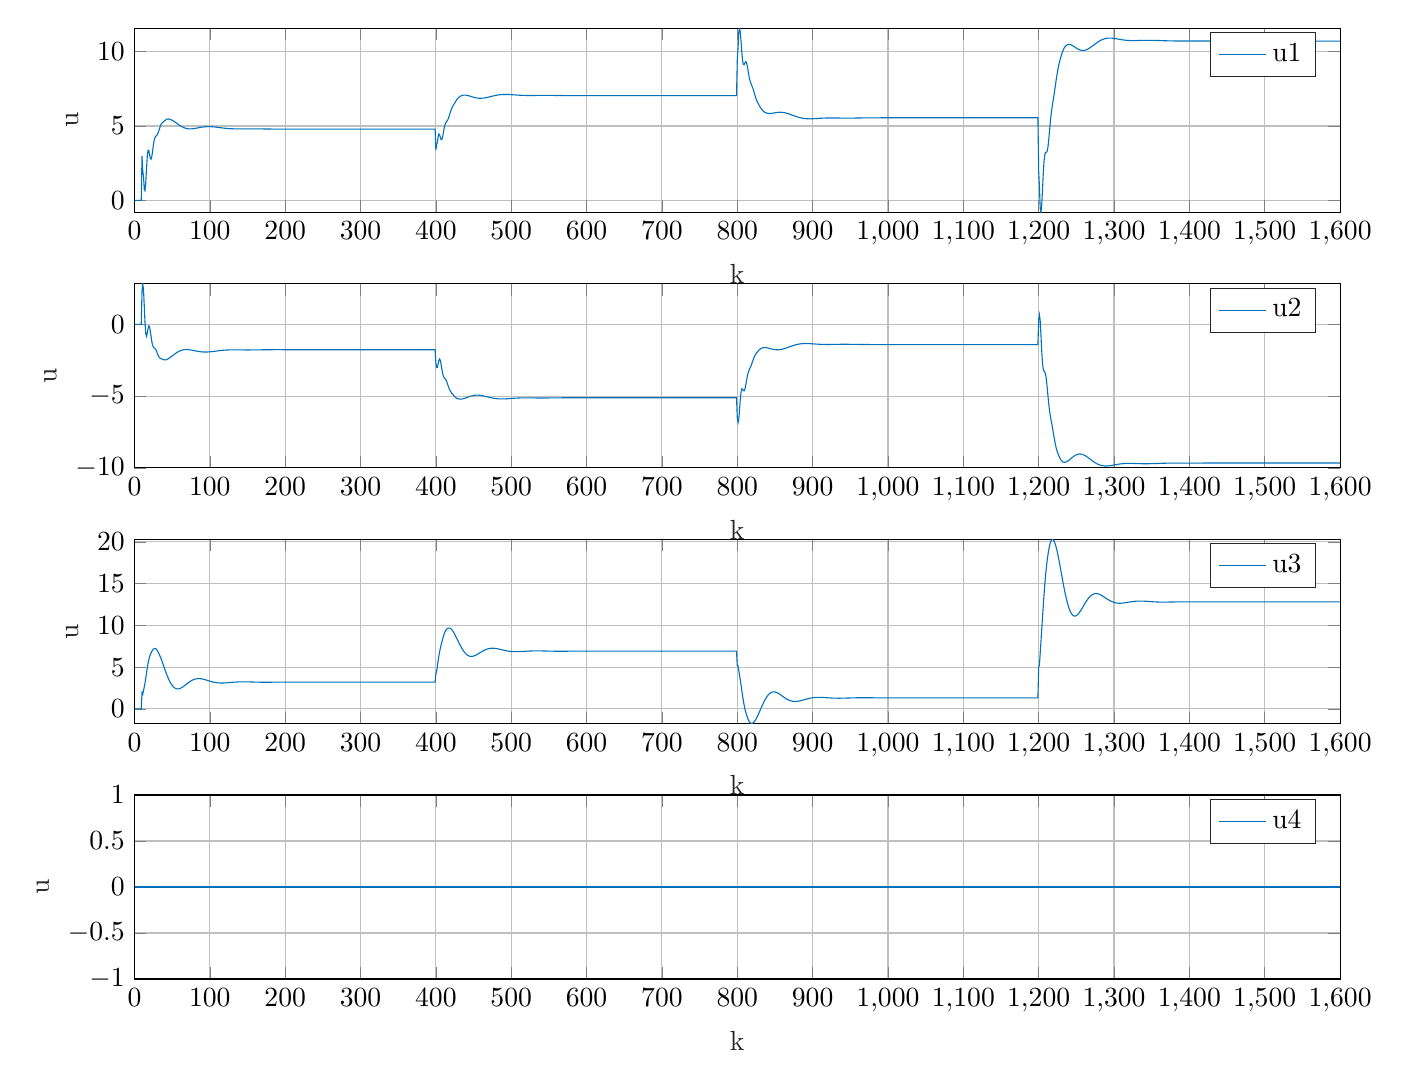
\begin{tikzpicture}

\begin{axis}[%
width=6.028in,
height=0.92in,
at={(1.011in,4.476in)},
scale only axis,
xmin=0,
xmax=1600,
xlabel style={font=\color{white!15!black}},
xlabel={k},
ymin=-0.80079,
ymax=11.581,
ylabel style={font=\color{white!15!black}},
ylabel={u},
axis background/.style={fill=white},
xmajorgrids,
ymajorgrids,
legend style={legend cell align=left, align=left, draw=white!15!black}
]
\addplot [color=mycolor1]
  table[row sep=crcr]{%
1	0\\
2	0\\
3	0\\
4	0\\
5	0\\
6	0\\
7	0\\
8	0\\
9	0\\
10	2.9925\\
11	1.9651\\
12	1.5955\\
13	0.75662\\
14	0.65506\\
15	1.2101\\
16	2.1365\\
17	2.958\\
18	3.3746\\
19	3.3551\\
20	3.0879\\
21	2.8302\\
22	2.768\\
23	2.9489\\
24	3.2981\\
25	3.6867\\
26	4.0042\\
27	4.2022\\
28	4.297\\
29	4.3433\\
30	4.3982\\
31	4.4947\\
32	4.6344\\
33	4.7954\\
34	4.9491\\
35	5.0742\\
36	5.164\\
37	5.2248\\
38	5.2692\\
39	5.3087\\
40	5.3494\\
41	5.3907\\
42	5.4279\\
43	5.4557\\
44	5.471\\
45	5.4734\\
46	5.4656\\
47	5.4507\\
48	5.4317\\
49	5.4101\\
50	5.3862\\
51	5.3596\\
52	5.3298\\
53	5.2967\\
54	5.2609\\
55	5.2236\\
56	5.1858\\
57	5.1485\\
58	5.1121\\
59	5.0771\\
60	5.0435\\
61	5.0115\\
62	4.9812\\
63	4.9529\\
64	4.9269\\
65	4.9034\\
66	4.8826\\
67	4.8645\\
68	4.8492\\
69	4.8365\\
70	4.8264\\
71	4.8188\\
72	4.8135\\
73	4.8104\\
74	4.8095\\
75	4.8105\\
76	4.8133\\
77	4.8176\\
78	4.8233\\
79	4.8302\\
80	4.838\\
81	4.8465\\
82	4.8556\\
83	4.865\\
84	4.8747\\
85	4.8843\\
86	4.8939\\
87	4.9031\\
88	4.9119\\
89	4.9202\\
90	4.9279\\
91	4.9349\\
92	4.941\\
93	4.9464\\
94	4.9508\\
95	4.9544\\
96	4.957\\
97	4.9587\\
98	4.9595\\
99	4.9594\\
100	4.9585\\
101	4.9568\\
102	4.9542\\
103	4.951\\
104	4.9472\\
105	4.9427\\
106	4.9377\\
107	4.9323\\
108	4.9265\\
109	4.9204\\
110	4.9141\\
111	4.9076\\
112	4.901\\
113	4.8943\\
114	4.8877\\
115	4.8812\\
116	4.8747\\
117	4.8685\\
118	4.8624\\
119	4.8566\\
120	4.8511\\
121	4.8459\\
122	4.841\\
123	4.8365\\
124	4.8323\\
125	4.8285\\
126	4.825\\
127	4.8219\\
128	4.8192\\
129	4.8167\\
130	4.8147\\
131	4.8129\\
132	4.8115\\
133	4.8103\\
134	4.8094\\
135	4.8087\\
136	4.8082\\
137	4.8079\\
138	4.8078\\
139	4.8079\\
140	4.808\\
141	4.8083\\
142	4.8086\\
143	4.809\\
144	4.8094\\
145	4.8098\\
146	4.8102\\
147	4.8107\\
148	4.811\\
149	4.8114\\
150	4.8117\\
151	4.8119\\
152	4.8121\\
153	4.8122\\
154	4.8122\\
155	4.8121\\
156	4.812\\
157	4.8118\\
158	4.8115\\
159	4.8112\\
160	4.8107\\
161	4.8102\\
162	4.8097\\
163	4.8091\\
164	4.8084\\
165	4.8078\\
166	4.807\\
167	4.8063\\
168	4.8055\\
169	4.8047\\
170	4.8039\\
171	4.8032\\
172	4.8024\\
173	4.8016\\
174	4.8009\\
175	4.8001\\
176	4.7994\\
177	4.7987\\
178	4.7981\\
179	4.7975\\
180	4.7969\\
181	4.7964\\
182	4.7959\\
183	4.7955\\
184	4.7951\\
185	4.7948\\
186	4.7945\\
187	4.7942\\
188	4.794\\
189	4.7938\\
190	4.7936\\
191	4.7935\\
192	4.7934\\
193	4.7934\\
194	4.7933\\
195	4.7933\\
196	4.7934\\
197	4.7934\\
198	4.7934\\
199	4.7935\\
200	4.7936\\
201	4.7937\\
202	4.7938\\
203	4.7939\\
204	4.7939\\
205	4.794\\
206	4.7941\\
207	4.7942\\
208	4.7943\\
209	4.7944\\
210	4.7945\\
211	4.7945\\
212	4.7946\\
213	4.7946\\
214	4.7947\\
215	4.7947\\
216	4.7947\\
217	4.7947\\
218	4.7947\\
219	4.7947\\
220	4.7947\\
221	4.7947\\
222	4.7947\\
223	4.7947\\
224	4.7946\\
225	4.7946\\
226	4.7946\\
227	4.7945\\
228	4.7945\\
229	4.7944\\
230	4.7944\\
231	4.7943\\
232	4.7943\\
233	4.7942\\
234	4.7942\\
235	4.7941\\
236	4.7941\\
237	4.7941\\
238	4.794\\
239	4.794\\
240	4.794\\
241	4.794\\
242	4.7939\\
243	4.7939\\
244	4.7939\\
245	4.7939\\
246	4.7939\\
247	4.7939\\
248	4.7939\\
249	4.7939\\
250	4.7939\\
251	4.7939\\
252	4.794\\
253	4.794\\
254	4.794\\
255	4.794\\
256	4.794\\
257	4.7941\\
258	4.7941\\
259	4.7941\\
260	4.7941\\
261	4.7942\\
262	4.7942\\
263	4.7942\\
264	4.7942\\
265	4.7943\\
266	4.7943\\
267	4.7943\\
268	4.7943\\
269	4.7944\\
270	4.7944\\
271	4.7944\\
272	4.7944\\
273	4.7944\\
274	4.7944\\
275	4.7944\\
276	4.7945\\
277	4.7945\\
278	4.7945\\
279	4.7945\\
280	4.7945\\
281	4.7945\\
282	4.7945\\
283	4.7945\\
284	4.7945\\
285	4.7945\\
286	4.7945\\
287	4.7945\\
288	4.7945\\
289	4.7945\\
290	4.7945\\
291	4.7945\\
292	4.7945\\
293	4.7945\\
294	4.7945\\
295	4.7945\\
296	4.7945\\
297	4.7945\\
298	4.7945\\
299	4.7945\\
300	4.7945\\
301	4.7945\\
302	4.7945\\
303	4.7945\\
304	4.7945\\
305	4.7945\\
306	4.7945\\
307	4.7945\\
308	4.7945\\
309	4.7945\\
310	4.7945\\
311	4.7945\\
312	4.7945\\
313	4.7945\\
314	4.7945\\
315	4.7946\\
316	4.7946\\
317	4.7946\\
318	4.7946\\
319	4.7946\\
320	4.7946\\
321	4.7946\\
322	4.7946\\
323	4.7946\\
324	4.7946\\
325	4.7946\\
326	4.7946\\
327	4.7946\\
328	4.7946\\
329	4.7946\\
330	4.7946\\
331	4.7946\\
332	4.7946\\
333	4.7946\\
334	4.7946\\
335	4.7946\\
336	4.7946\\
337	4.7946\\
338	4.7946\\
339	4.7946\\
340	4.7946\\
341	4.7946\\
342	4.7946\\
343	4.7946\\
344	4.7946\\
345	4.7946\\
346	4.7946\\
347	4.7946\\
348	4.7946\\
349	4.7946\\
350	4.7946\\
351	4.7946\\
352	4.7946\\
353	4.7946\\
354	4.7946\\
355	4.7946\\
356	4.7946\\
357	4.7946\\
358	4.7946\\
359	4.7946\\
360	4.7946\\
361	4.7946\\
362	4.7946\\
363	4.7946\\
364	4.7946\\
365	4.7946\\
366	4.7946\\
367	4.7946\\
368	4.7946\\
369	4.7946\\
370	4.7946\\
371	4.7946\\
372	4.7946\\
373	4.7946\\
374	4.7946\\
375	4.7946\\
376	4.7946\\
377	4.7946\\
378	4.7946\\
379	4.7946\\
380	4.7946\\
381	4.7946\\
382	4.7946\\
383	4.7946\\
384	4.7946\\
385	4.7946\\
386	4.7946\\
387	4.7946\\
388	4.7946\\
389	4.7946\\
390	4.7946\\
391	4.7946\\
392	4.7946\\
393	4.7946\\
394	4.7946\\
395	4.7946\\
396	4.7946\\
397	4.7946\\
398	4.7946\\
399	4.7946\\
400	3.3981\\
401	3.7633\\
402	3.8863\\
403	4.2873\\
404	4.4569\\
405	4.4063\\
406	4.2239\\
407	4.0828\\
408	4.0959\\
409	4.2779\\
410	4.5608\\
411	4.849\\
412	5.0721\\
413	5.2098\\
414	5.2872\\
415	5.3496\\
416	5.4359\\
417	5.5622\\
418	5.7211\\
419	5.8911\\
420	6.0501\\
421	6.185\\
422	6.2943\\
423	6.3853\\
424	6.4681\\
425	6.55\\
426	6.6332\\
427	6.7152\\
428	6.7913\\
429	6.8575\\
430	6.9119\\
431	6.9549\\
432	6.9888\\
433	7.0161\\
434	7.0384\\
435	7.0566\\
436	7.0704\\
437	7.0794\\
438	7.0833\\
439	7.0821\\
440	7.0768\\
441	7.0681\\
442	7.0571\\
443	7.0444\\
444	7.0305\\
445	7.0158\\
446	7.0004\\
447	6.9846\\
448	6.9687\\
449	6.9531\\
450	6.9382\\
451	6.9243\\
452	6.9117\\
453	6.9005\\
454	6.8909\\
455	6.8829\\
456	6.8765\\
457	6.8719\\
458	6.869\\
459	6.8678\\
460	6.8684\\
461	6.8707\\
462	6.8745\\
463	6.8798\\
464	6.8865\\
465	6.8944\\
466	6.9034\\
467	6.9133\\
468	6.9241\\
469	6.9355\\
470	6.9474\\
471	6.9597\\
472	6.9723\\
473	6.9849\\
474	6.9975\\
475	7.0099\\
476	7.022\\
477	7.0337\\
478	7.0449\\
479	7.0556\\
480	7.0656\\
481	7.0749\\
482	7.0835\\
483	7.0913\\
484	7.0982\\
485	7.1044\\
486	7.1097\\
487	7.1141\\
488	7.1178\\
489	7.1206\\
490	7.1227\\
491	7.124\\
492	7.1246\\
493	7.1246\\
494	7.124\\
495	7.1229\\
496	7.1212\\
497	7.1191\\
498	7.1166\\
499	7.1139\\
500	7.1108\\
501	7.1075\\
502	7.1041\\
503	7.1005\\
504	7.0969\\
505	7.0933\\
506	7.0897\\
507	7.0862\\
508	7.0828\\
509	7.0795\\
510	7.0763\\
511	7.0734\\
512	7.0706\\
513	7.0681\\
514	7.0657\\
515	7.0636\\
516	7.0617\\
517	7.0601\\
518	7.0587\\
519	7.0575\\
520	7.0565\\
521	7.0557\\
522	7.0551\\
523	7.0547\\
524	7.0545\\
525	7.0544\\
526	7.0544\\
527	7.0546\\
528	7.0549\\
529	7.0552\\
530	7.0557\\
531	7.0561\\
532	7.0566\\
533	7.0572\\
534	7.0577\\
535	7.0582\\
536	7.0587\\
537	7.0592\\
538	7.0597\\
539	7.0601\\
540	7.0604\\
541	7.0607\\
542	7.0609\\
543	7.0611\\
544	7.0612\\
545	7.0612\\
546	7.0612\\
547	7.061\\
548	7.0609\\
549	7.0606\\
550	7.0603\\
551	7.0599\\
552	7.0595\\
553	7.0591\\
554	7.0586\\
555	7.058\\
556	7.0575\\
557	7.0569\\
558	7.0562\\
559	7.0556\\
560	7.055\\
561	7.0543\\
562	7.0537\\
563	7.0531\\
564	7.0525\\
565	7.0518\\
566	7.0513\\
567	7.0507\\
568	7.0501\\
569	7.0496\\
570	7.0491\\
571	7.0487\\
572	7.0483\\
573	7.0479\\
574	7.0475\\
575	7.0472\\
576	7.0469\\
577	7.0466\\
578	7.0464\\
579	7.0462\\
580	7.046\\
581	7.0458\\
582	7.0457\\
583	7.0456\\
584	7.0455\\
585	7.0455\\
586	7.0454\\
587	7.0454\\
588	7.0454\\
589	7.0453\\
590	7.0453\\
591	7.0454\\
592	7.0454\\
593	7.0454\\
594	7.0454\\
595	7.0454\\
596	7.0454\\
597	7.0455\\
598	7.0455\\
599	7.0455\\
600	7.0455\\
601	7.0455\\
602	7.0455\\
603	7.0455\\
604	7.0455\\
605	7.0454\\
606	7.0454\\
607	7.0454\\
608	7.0453\\
609	7.0453\\
610	7.0452\\
611	7.0452\\
612	7.0451\\
613	7.0451\\
614	7.045\\
615	7.045\\
616	7.0449\\
617	7.0448\\
618	7.0448\\
619	7.0447\\
620	7.0446\\
621	7.0446\\
622	7.0445\\
623	7.0444\\
624	7.0444\\
625	7.0443\\
626	7.0443\\
627	7.0442\\
628	7.0442\\
629	7.0441\\
630	7.0441\\
631	7.044\\
632	7.044\\
633	7.044\\
634	7.044\\
635	7.0439\\
636	7.0439\\
637	7.0439\\
638	7.0439\\
639	7.0439\\
640	7.0439\\
641	7.0439\\
642	7.0439\\
643	7.0439\\
644	7.0439\\
645	7.0439\\
646	7.0439\\
647	7.0439\\
648	7.0439\\
649	7.0439\\
650	7.0439\\
651	7.0439\\
652	7.0439\\
653	7.0439\\
654	7.0439\\
655	7.0439\\
656	7.044\\
657	7.044\\
658	7.044\\
659	7.044\\
660	7.044\\
661	7.044\\
662	7.044\\
663	7.044\\
664	7.044\\
665	7.044\\
666	7.044\\
667	7.044\\
668	7.044\\
669	7.044\\
670	7.044\\
671	7.044\\
672	7.044\\
673	7.044\\
674	7.044\\
675	7.044\\
676	7.044\\
677	7.044\\
678	7.044\\
679	7.044\\
680	7.044\\
681	7.044\\
682	7.044\\
683	7.044\\
684	7.044\\
685	7.044\\
686	7.044\\
687	7.044\\
688	7.044\\
689	7.044\\
690	7.044\\
691	7.044\\
692	7.044\\
693	7.044\\
694	7.044\\
695	7.044\\
696	7.044\\
697	7.044\\
698	7.044\\
699	7.044\\
700	7.044\\
701	7.044\\
702	7.044\\
703	7.044\\
704	7.044\\
705	7.044\\
706	7.044\\
707	7.044\\
708	7.044\\
709	7.044\\
710	7.044\\
711	7.044\\
712	7.044\\
713	7.044\\
714	7.044\\
715	7.044\\
716	7.044\\
717	7.044\\
718	7.044\\
719	7.044\\
720	7.044\\
721	7.044\\
722	7.044\\
723	7.044\\
724	7.044\\
725	7.044\\
726	7.044\\
727	7.044\\
728	7.044\\
729	7.044\\
730	7.044\\
731	7.044\\
732	7.044\\
733	7.044\\
734	7.044\\
735	7.0441\\
736	7.0441\\
737	7.0441\\
738	7.0441\\
739	7.0441\\
740	7.0441\\
741	7.0441\\
742	7.0441\\
743	7.0441\\
744	7.0441\\
745	7.0441\\
746	7.0441\\
747	7.0441\\
748	7.0441\\
749	7.0441\\
750	7.0441\\
751	7.0441\\
752	7.0441\\
753	7.0441\\
754	7.0441\\
755	7.0441\\
756	7.0441\\
757	7.0441\\
758	7.0441\\
759	7.0441\\
760	7.0441\\
761	7.0441\\
762	7.0441\\
763	7.0441\\
764	7.0441\\
765	7.0441\\
766	7.0441\\
767	7.0441\\
768	7.0441\\
769	7.0441\\
770	7.0441\\
771	7.0441\\
772	7.0441\\
773	7.0441\\
774	7.0441\\
775	7.0441\\
776	7.0441\\
777	7.0441\\
778	7.0441\\
779	7.0441\\
780	7.0441\\
781	7.0441\\
782	7.0441\\
783	7.0441\\
784	7.0441\\
785	7.0441\\
786	7.0441\\
787	7.0441\\
788	7.0441\\
789	7.0441\\
790	7.0441\\
791	7.0441\\
792	7.0441\\
793	7.0441\\
794	7.0441\\
795	7.0441\\
796	7.0441\\
797	7.0441\\
798	7.0441\\
799	7.0441\\
800	9.4381\\
801	10.219\\
802	11.315\\
803	11.581\\
804	11.328\\
805	10.688\\
806	9.971\\
807	9.4157\\
808	9.1428\\
809	9.1245\\
810	9.2341\\
811	9.3235\\
812	9.291\\
813	9.1127\\
814	8.8314\\
815	8.5201\\
816	8.243\\
817	8.0309\\
818	7.8781\\
819	7.7564\\
820	7.6342\\
821	7.4918\\
822	7.3268\\
823	7.1504\\
824	6.9787\\
825	6.8245\\
826	6.693\\
827	6.5818\\
828	6.4846\\
829	6.3948\\
830	6.3088\\
831	6.2264\\
832	6.1499\\
833	6.0823\\
834	6.0254\\
835	5.9794\\
836	5.9431\\
837	5.9145\\
838	5.8918\\
839	5.8737\\
840	5.8599\\
841	5.8502\\
842	5.8448\\
843	5.8434\\
844	5.8456\\
845	5.8504\\
846	5.8571\\
847	5.865\\
848	5.8734\\
849	5.882\\
850	5.8905\\
851	5.8987\\
852	5.9062\\
853	5.9129\\
854	5.9184\\
855	5.9225\\
856	5.925\\
857	5.9258\\
858	5.9247\\
859	5.9218\\
860	5.9171\\
861	5.9107\\
862	5.9026\\
863	5.8927\\
864	5.8814\\
865	5.8686\\
866	5.8544\\
867	5.8391\\
868	5.8228\\
869	5.8057\\
870	5.7879\\
871	5.7695\\
872	5.7509\\
873	5.7321\\
874	5.7132\\
875	5.6945\\
876	5.6761\\
877	5.6581\\
878	5.6406\\
879	5.6238\\
880	5.6078\\
881	5.5925\\
882	5.5782\\
883	5.5649\\
884	5.5526\\
885	5.5413\\
886	5.5312\\
887	5.5221\\
888	5.514\\
889	5.5071\\
890	5.5012\\
891	5.4963\\
892	5.4923\\
893	5.4893\\
894	5.4872\\
895	5.4858\\
896	5.4853\\
897	5.4854\\
898	5.4861\\
899	5.4873\\
900	5.4891\\
901	5.4912\\
902	5.4937\\
903	5.4965\\
904	5.4995\\
905	5.5026\\
906	5.5059\\
907	5.5092\\
908	5.5124\\
909	5.5157\\
910	5.5188\\
911	5.5218\\
912	5.5247\\
913	5.5274\\
914	5.5299\\
915	5.5322\\
916	5.5342\\
917	5.536\\
918	5.5376\\
919	5.539\\
920	5.5401\\
921	5.541\\
922	5.5416\\
923	5.5421\\
924	5.5423\\
925	5.5424\\
926	5.5424\\
927	5.5421\\
928	5.5418\\
929	5.5413\\
930	5.5408\\
931	5.5402\\
932	5.5395\\
933	5.5388\\
934	5.5381\\
935	5.5373\\
936	5.5366\\
937	5.5359\\
938	5.5353\\
939	5.5347\\
940	5.5341\\
941	5.5336\\
942	5.5332\\
943	5.5329\\
944	5.5327\\
945	5.5325\\
946	5.5324\\
947	5.5325\\
948	5.5326\\
949	5.5327\\
950	5.533\\
951	5.5334\\
952	5.5338\\
953	5.5343\\
954	5.5348\\
955	5.5354\\
956	5.5361\\
957	5.5367\\
958	5.5375\\
959	5.5382\\
960	5.539\\
961	5.5398\\
962	5.5406\\
963	5.5414\\
964	5.5422\\
965	5.543\\
966	5.5438\\
967	5.5445\\
968	5.5453\\
969	5.546\\
970	5.5466\\
971	5.5473\\
972	5.5479\\
973	5.5485\\
974	5.549\\
975	5.5495\\
976	5.55\\
977	5.5504\\
978	5.5508\\
979	5.5512\\
980	5.5515\\
981	5.5518\\
982	5.552\\
983	5.5522\\
984	5.5524\\
985	5.5526\\
986	5.5527\\
987	5.5529\\
988	5.553\\
989	5.5531\\
990	5.5531\\
991	5.5532\\
992	5.5532\\
993	5.5533\\
994	5.5533\\
995	5.5533\\
996	5.5534\\
997	5.5534\\
998	5.5534\\
999	5.5534\\
1000	5.5535\\
1001	5.5535\\
1002	5.5535\\
1003	5.5536\\
1004	5.5536\\
1005	5.5537\\
1006	5.5537\\
1007	5.5538\\
1008	5.5539\\
1009	5.5539\\
1010	5.554\\
1011	5.5541\\
1012	5.5542\\
1013	5.5543\\
1014	5.5544\\
1015	5.5545\\
1016	5.5546\\
1017	5.5547\\
1018	5.5548\\
1019	5.5549\\
1020	5.555\\
1021	5.5551\\
1022	5.5552\\
1023	5.5553\\
1024	5.5554\\
1025	5.5555\\
1026	5.5556\\
1027	5.5557\\
1028	5.5557\\
1029	5.5558\\
1030	5.5559\\
1031	5.556\\
1032	5.556\\
1033	5.5561\\
1034	5.5561\\
1035	5.5562\\
1036	5.5562\\
1037	5.5563\\
1038	5.5563\\
1039	5.5563\\
1040	5.5564\\
1041	5.5564\\
1042	5.5564\\
1043	5.5564\\
1044	5.5564\\
1045	5.5564\\
1046	5.5564\\
1047	5.5565\\
1048	5.5565\\
1049	5.5565\\
1050	5.5565\\
1051	5.5565\\
1052	5.5564\\
1053	5.5564\\
1054	5.5564\\
1055	5.5564\\
1056	5.5564\\
1057	5.5564\\
1058	5.5564\\
1059	5.5564\\
1060	5.5564\\
1061	5.5564\\
1062	5.5564\\
1063	5.5564\\
1064	5.5564\\
1065	5.5564\\
1066	5.5564\\
1067	5.5564\\
1068	5.5564\\
1069	5.5564\\
1070	5.5564\\
1071	5.5564\\
1072	5.5564\\
1073	5.5564\\
1074	5.5564\\
1075	5.5564\\
1076	5.5564\\
1077	5.5564\\
1078	5.5564\\
1079	5.5564\\
1080	5.5564\\
1081	5.5564\\
1082	5.5565\\
1083	5.5565\\
1084	5.5565\\
1085	5.5565\\
1086	5.5565\\
1087	5.5565\\
1088	5.5565\\
1089	5.5565\\
1090	5.5565\\
1091	5.5565\\
1092	5.5565\\
1093	5.5565\\
1094	5.5565\\
1095	5.5565\\
1096	5.5565\\
1097	5.5565\\
1098	5.5565\\
1099	5.5565\\
1100	5.5565\\
1101	5.5565\\
1102	5.5565\\
1103	5.5565\\
1104	5.5565\\
1105	5.5565\\
1106	5.5565\\
1107	5.5565\\
1108	5.5565\\
1109	5.5565\\
1110	5.5565\\
1111	5.5565\\
1112	5.5565\\
1113	5.5564\\
1114	5.5564\\
1115	5.5564\\
1116	5.5564\\
1117	5.5564\\
1118	5.5564\\
1119	5.5564\\
1120	5.5564\\
1121	5.5564\\
1122	5.5564\\
1123	5.5564\\
1124	5.5564\\
1125	5.5564\\
1126	5.5564\\
1127	5.5564\\
1128	5.5564\\
1129	5.5564\\
1130	5.5564\\
1131	5.5564\\
1132	5.5564\\
1133	5.5564\\
1134	5.5564\\
1135	5.5564\\
1136	5.5564\\
1137	5.5564\\
1138	5.5564\\
1139	5.5564\\
1140	5.5564\\
1141	5.5564\\
1142	5.5564\\
1143	5.5564\\
1144	5.5564\\
1145	5.5564\\
1146	5.5564\\
1147	5.5564\\
1148	5.5564\\
1149	5.5564\\
1150	5.5564\\
1151	5.5564\\
1152	5.5564\\
1153	5.5564\\
1154	5.5564\\
1155	5.5564\\
1156	5.5564\\
1157	5.5564\\
1158	5.5564\\
1159	5.5564\\
1160	5.5564\\
1161	5.5564\\
1162	5.5564\\
1163	5.5564\\
1164	5.5564\\
1165	5.5564\\
1166	5.5564\\
1167	5.5564\\
1168	5.5564\\
1169	5.5564\\
1170	5.5564\\
1171	5.5564\\
1172	5.5564\\
1173	5.5564\\
1174	5.5564\\
1175	5.5564\\
1176	5.5564\\
1177	5.5564\\
1178	5.5564\\
1179	5.5564\\
1180	5.5564\\
1181	5.5564\\
1182	5.5564\\
1183	5.5564\\
1184	5.5564\\
1185	5.5564\\
1186	5.5564\\
1187	5.5564\\
1188	5.5564\\
1189	5.5564\\
1190	5.5564\\
1191	5.5564\\
1192	5.5564\\
1193	5.5564\\
1194	5.5564\\
1195	5.5564\\
1196	5.5564\\
1197	5.5564\\
1198	5.5564\\
1199	5.5564\\
1200	1.9654\\
1201	0.93482\\
1202	-0.54652\\
1203	-0.80079\\
1204	-0.34519\\
1205	0.62807\\
1206	1.6967\\
1207	2.5523\\
1208	3.0444\\
1209	3.2145\\
1210	3.2281\\
1211	3.2762\\
1212	3.4878\\
1213	3.8915\\
1214	4.4301\\
1215	5.0074\\
1216	5.539\\
1217	5.9837\\
1218	6.3473\\
1219	6.665\\
1220	6.9766\\
1221	7.3067\\
1222	7.6578\\
1223	8.0151\\
1224	8.3573\\
1225	8.6673\\
1226	8.9382\\
1227	9.1727\\
1228	9.3792\\
1229	9.5661\\
1230	9.7383\\
1231	9.8965\\
1232	10.038\\
1233	10.16\\
1234	10.259\\
1235	10.337\\
1236	10.395\\
1237	10.438\\
1238	10.466\\
1239	10.484\\
1240	10.492\\
1241	10.491\\
1242	10.481\\
1243	10.464\\
1244	10.44\\
1245	10.411\\
1246	10.379\\
1247	10.345\\
1248	10.311\\
1249	10.277\\
1250	10.244\\
1251	10.213\\
1252	10.184\\
1253	10.158\\
1254	10.136\\
1255	10.117\\
1256	10.103\\
1257	10.093\\
1258	10.088\\
1259	10.088\\
1260	10.092\\
1261	10.101\\
1262	10.113\\
1263	10.13\\
1264	10.151\\
1265	10.175\\
1266	10.202\\
1267	10.232\\
1268	10.265\\
1269	10.299\\
1270	10.335\\
1271	10.373\\
1272	10.411\\
1273	10.449\\
1274	10.488\\
1275	10.526\\
1276	10.563\\
1277	10.6\\
1278	10.635\\
1279	10.669\\
1280	10.701\\
1281	10.731\\
1282	10.759\\
1283	10.785\\
1284	10.809\\
1285	10.83\\
1286	10.849\\
1287	10.865\\
1288	10.879\\
1289	10.891\\
1290	10.901\\
1291	10.908\\
1292	10.913\\
1293	10.916\\
1294	10.918\\
1295	10.917\\
1296	10.915\\
1297	10.912\\
1298	10.908\\
1299	10.902\\
1300	10.895\\
1301	10.888\\
1302	10.88\\
1303	10.871\\
1304	10.863\\
1305	10.854\\
1306	10.845\\
1307	10.836\\
1308	10.827\\
1309	10.818\\
1310	10.81\\
1311	10.802\\
1312	10.794\\
1313	10.787\\
1314	10.781\\
1315	10.775\\
1316	10.77\\
1317	10.765\\
1318	10.761\\
1319	10.758\\
1320	10.755\\
1321	10.752\\
1322	10.751\\
1323	10.749\\
1324	10.749\\
1325	10.748\\
1326	10.748\\
1327	10.749\\
1328	10.749\\
1329	10.75\\
1330	10.751\\
1331	10.753\\
1332	10.754\\
1333	10.755\\
1334	10.757\\
1335	10.759\\
1336	10.76\\
1337	10.761\\
1338	10.763\\
1339	10.764\\
1340	10.765\\
1341	10.766\\
1342	10.767\\
1343	10.768\\
1344	10.768\\
1345	10.768\\
1346	10.768\\
1347	10.768\\
1348	10.768\\
1349	10.767\\
1350	10.766\\
1351	10.765\\
1352	10.764\\
1353	10.763\\
1354	10.762\\
1355	10.76\\
1356	10.759\\
1357	10.757\\
1358	10.756\\
1359	10.754\\
1360	10.752\\
1361	10.75\\
1362	10.748\\
1363	10.747\\
1364	10.745\\
1365	10.743\\
1366	10.741\\
1367	10.74\\
1368	10.738\\
1369	10.736\\
1370	10.735\\
1371	10.734\\
1372	10.732\\
1373	10.731\\
1374	10.73\\
1375	10.729\\
1376	10.728\\
1377	10.727\\
1378	10.726\\
1379	10.726\\
1380	10.725\\
1381	10.724\\
1382	10.724\\
1383	10.724\\
1384	10.723\\
1385	10.723\\
1386	10.723\\
1387	10.722\\
1388	10.722\\
1389	10.722\\
1390	10.722\\
1391	10.722\\
1392	10.722\\
1393	10.722\\
1394	10.722\\
1395	10.722\\
1396	10.722\\
1397	10.722\\
1398	10.722\\
1399	10.722\\
1400	10.722\\
1401	10.722\\
1402	10.722\\
1403	10.722\\
1404	10.722\\
1405	10.722\\
1406	10.722\\
1407	10.722\\
1408	10.721\\
1409	10.721\\
1410	10.721\\
1411	10.721\\
1412	10.721\\
1413	10.721\\
1414	10.72\\
1415	10.72\\
1416	10.72\\
1417	10.72\\
1418	10.72\\
1419	10.719\\
1420	10.719\\
1421	10.719\\
1422	10.719\\
1423	10.719\\
1424	10.718\\
1425	10.718\\
1426	10.718\\
1427	10.718\\
1428	10.718\\
1429	10.718\\
1430	10.717\\
1431	10.717\\
1432	10.717\\
1433	10.717\\
1434	10.717\\
1435	10.717\\
1436	10.717\\
1437	10.717\\
1438	10.717\\
1439	10.717\\
1440	10.717\\
1441	10.717\\
1442	10.717\\
1443	10.717\\
1444	10.717\\
1445	10.717\\
1446	10.717\\
1447	10.717\\
1448	10.717\\
1449	10.717\\
1450	10.717\\
1451	10.717\\
1452	10.717\\
1453	10.717\\
1454	10.717\\
1455	10.717\\
1456	10.717\\
1457	10.717\\
1458	10.717\\
1459	10.717\\
1460	10.717\\
1461	10.717\\
1462	10.717\\
1463	10.717\\
1464	10.717\\
1465	10.717\\
1466	10.717\\
1467	10.717\\
1468	10.717\\
1469	10.717\\
1470	10.717\\
1471	10.717\\
1472	10.717\\
1473	10.717\\
1474	10.717\\
1475	10.717\\
1476	10.717\\
1477	10.717\\
1478	10.717\\
1479	10.717\\
1480	10.717\\
1481	10.717\\
1482	10.717\\
1483	10.717\\
1484	10.717\\
1485	10.717\\
1486	10.717\\
1487	10.717\\
1488	10.717\\
1489	10.717\\
1490	10.717\\
1491	10.717\\
1492	10.717\\
1493	10.717\\
1494	10.717\\
1495	10.717\\
1496	10.717\\
1497	10.717\\
1498	10.717\\
1499	10.717\\
1500	10.717\\
1501	10.717\\
1502	10.717\\
1503	10.717\\
1504	10.717\\
1505	10.717\\
1506	10.717\\
1507	10.717\\
1508	10.717\\
1509	10.717\\
1510	10.717\\
1511	10.717\\
1512	10.717\\
1513	10.717\\
1514	10.717\\
1515	10.717\\
1516	10.717\\
1517	10.717\\
1518	10.717\\
1519	10.717\\
1520	10.717\\
1521	10.717\\
1522	10.717\\
1523	10.717\\
1524	10.717\\
1525	10.717\\
1526	10.717\\
1527	10.717\\
1528	10.717\\
1529	10.717\\
1530	10.717\\
1531	10.717\\
1532	10.717\\
1533	10.717\\
1534	10.717\\
1535	10.717\\
1536	10.717\\
1537	10.717\\
1538	10.717\\
1539	10.717\\
1540	10.717\\
1541	10.717\\
1542	10.717\\
1543	10.717\\
1544	10.717\\
1545	10.717\\
1546	10.717\\
1547	10.717\\
1548	10.717\\
1549	10.717\\
1550	10.717\\
1551	10.717\\
1552	10.717\\
1553	10.717\\
1554	10.717\\
1555	10.717\\
1556	10.717\\
1557	10.717\\
1558	10.717\\
1559	10.717\\
1560	10.717\\
1561	10.717\\
1562	10.717\\
1563	10.717\\
1564	10.717\\
1565	10.717\\
1566	10.717\\
1567	10.717\\
1568	10.717\\
1569	10.717\\
1570	10.717\\
1571	10.717\\
1572	10.717\\
1573	10.717\\
1574	10.717\\
1575	10.717\\
1576	10.717\\
1577	10.717\\
1578	10.717\\
1579	10.717\\
1580	10.717\\
1581	10.717\\
1582	10.717\\
1583	10.717\\
1584	10.717\\
1585	10.717\\
1586	10.717\\
1587	10.717\\
1588	10.717\\
1589	10.717\\
1590	10.717\\
1591	10.717\\
1592	10.717\\
1593	10.717\\
1594	10.717\\
1595	10.717\\
1596	10.717\\
1597	10.717\\
1598	10.717\\
1599	10.717\\
1600	10.717\\
};
\addlegendentry{u1}

\end{axis}

\begin{axis}[%
width=6.028in,
height=0.92in,
at={(1.011in,3.198in)},
scale only axis,
xmin=0,
xmax=1600,
xlabel style={font=\color{white!15!black}},
xlabel={k},
ymin=-10,
ymax=2.8325,
ylabel style={font=\color{white!15!black}},
ylabel={u},
axis background/.style={fill=white},
xmajorgrids,
ymajorgrids,
legend style={legend cell align=left, align=left, draw=white!15!black}
]
\addplot [color=mycolor1]
  table[row sep=crcr]{%
1	0\\
2	0\\
3	0\\
4	0\\
5	0\\
6	0\\
7	0\\
8	0\\
9	0\\
10	2.32\\
11	2.8325\\
12	2.3958\\
13	1.2824\\
14	0.12599\\
15	-0.62141\\
16	-0.821\\
17	-0.61817\\
18	-0.29347\\
19	-0.098827\\
20	-0.15478\\
21	-0.43601\\
22	-0.82518\\
23	-1.1911\\
24	-1.4498\\
25	-1.5862\\
26	-1.6401\\
27	-1.6716\\
28	-1.7285\\
29	-1.8289\\
30	-1.9621\\
31	-2.1016\\
32	-2.2214\\
33	-2.3073\\
34	-2.3595\\
35	-2.3882\\
36	-2.4063\\
37	-2.4233\\
38	-2.442\\
39	-2.46\\
40	-2.4721\\
41	-2.4741\\
42	-2.4643\\
43	-2.444\\
44	-2.4162\\
45	-2.3844\\
46	-2.3508\\
47	-2.3163\\
48	-2.2808\\
49	-2.2439\\
50	-2.2052\\
51	-2.1649\\
52	-2.1239\\
53	-2.0832\\
54	-2.0437\\
55	-2.0061\\
56	-1.9709\\
57	-1.938\\
58	-1.9075\\
59	-1.8794\\
60	-1.8538\\
61	-1.831\\
62	-1.811\\
63	-1.794\\
64	-1.78\\
65	-1.769\\
66	-1.7607\\
67	-1.7551\\
68	-1.7519\\
69	-1.751\\
70	-1.7522\\
71	-1.7553\\
72	-1.7602\\
73	-1.7666\\
74	-1.7743\\
75	-1.7831\\
76	-1.7927\\
77	-1.803\\
78	-1.8136\\
79	-1.8245\\
80	-1.8354\\
81	-1.8463\\
82	-1.8568\\
83	-1.8669\\
84	-1.8764\\
85	-1.8853\\
86	-1.8934\\
87	-1.9007\\
88	-1.907\\
89	-1.9124\\
90	-1.9168\\
91	-1.9202\\
92	-1.9227\\
93	-1.9241\\
94	-1.9246\\
95	-1.9241\\
96	-1.9227\\
97	-1.9205\\
98	-1.9176\\
99	-1.9139\\
100	-1.9095\\
101	-1.9046\\
102	-1.8992\\
103	-1.8934\\
104	-1.8872\\
105	-1.8807\\
106	-1.874\\
107	-1.8673\\
108	-1.8604\\
109	-1.8536\\
110	-1.8468\\
111	-1.8401\\
112	-1.8337\\
113	-1.8274\\
114	-1.8214\\
115	-1.8157\\
116	-1.8103\\
117	-1.8053\\
118	-1.8006\\
119	-1.7963\\
120	-1.7924\\
121	-1.7888\\
122	-1.7857\\
123	-1.7829\\
124	-1.7805\\
125	-1.7784\\
126	-1.7767\\
127	-1.7753\\
128	-1.7742\\
129	-1.7734\\
130	-1.7729\\
131	-1.7725\\
132	-1.7724\\
133	-1.7725\\
134	-1.7727\\
135	-1.773\\
136	-1.7734\\
137	-1.7739\\
138	-1.7745\\
139	-1.7751\\
140	-1.7757\\
141	-1.7763\\
142	-1.7769\\
143	-1.7774\\
144	-1.7779\\
145	-1.7784\\
146	-1.7788\\
147	-1.7791\\
148	-1.7793\\
149	-1.7794\\
150	-1.7795\\
151	-1.7794\\
152	-1.7793\\
153	-1.7791\\
154	-1.7788\\
155	-1.7785\\
156	-1.778\\
157	-1.7775\\
158	-1.7769\\
159	-1.7763\\
160	-1.7756\\
161	-1.7749\\
162	-1.7742\\
163	-1.7734\\
164	-1.7726\\
165	-1.7718\\
166	-1.771\\
167	-1.7702\\
168	-1.7694\\
169	-1.7686\\
170	-1.7679\\
171	-1.7672\\
172	-1.7665\\
173	-1.7658\\
174	-1.7652\\
175	-1.7646\\
176	-1.7641\\
177	-1.7636\\
178	-1.7632\\
179	-1.7627\\
180	-1.7624\\
181	-1.7621\\
182	-1.7618\\
183	-1.7616\\
184	-1.7614\\
185	-1.7613\\
186	-1.7611\\
187	-1.7611\\
188	-1.761\\
189	-1.761\\
190	-1.761\\
191	-1.761\\
192	-1.7611\\
193	-1.7612\\
194	-1.7612\\
195	-1.7613\\
196	-1.7614\\
197	-1.7615\\
198	-1.7617\\
199	-1.7618\\
200	-1.7619\\
201	-1.762\\
202	-1.7621\\
203	-1.7622\\
204	-1.7623\\
205	-1.7624\\
206	-1.7624\\
207	-1.7625\\
208	-1.7626\\
209	-1.7626\\
210	-1.7627\\
211	-1.7627\\
212	-1.7627\\
213	-1.7627\\
214	-1.7627\\
215	-1.7627\\
216	-1.7627\\
217	-1.7627\\
218	-1.7626\\
219	-1.7626\\
220	-1.7626\\
221	-1.7625\\
222	-1.7625\\
223	-1.7624\\
224	-1.7624\\
225	-1.7623\\
226	-1.7623\\
227	-1.7622\\
228	-1.7622\\
229	-1.7621\\
230	-1.7621\\
231	-1.762\\
232	-1.762\\
233	-1.762\\
234	-1.7619\\
235	-1.7619\\
236	-1.7619\\
237	-1.7619\\
238	-1.7618\\
239	-1.7618\\
240	-1.7618\\
241	-1.7618\\
242	-1.7618\\
243	-1.7618\\
244	-1.7618\\
245	-1.7618\\
246	-1.7618\\
247	-1.7619\\
248	-1.7619\\
249	-1.7619\\
250	-1.7619\\
251	-1.7619\\
252	-1.762\\
253	-1.762\\
254	-1.762\\
255	-1.762\\
256	-1.7621\\
257	-1.7621\\
258	-1.7621\\
259	-1.7622\\
260	-1.7622\\
261	-1.7622\\
262	-1.7622\\
263	-1.7622\\
264	-1.7623\\
265	-1.7623\\
266	-1.7623\\
267	-1.7623\\
268	-1.7623\\
269	-1.7623\\
270	-1.7624\\
271	-1.7624\\
272	-1.7624\\
273	-1.7624\\
274	-1.7624\\
275	-1.7624\\
276	-1.7624\\
277	-1.7624\\
278	-1.7624\\
279	-1.7624\\
280	-1.7624\\
281	-1.7624\\
282	-1.7624\\
283	-1.7624\\
284	-1.7624\\
285	-1.7624\\
286	-1.7624\\
287	-1.7624\\
288	-1.7624\\
289	-1.7624\\
290	-1.7624\\
291	-1.7624\\
292	-1.7624\\
293	-1.7624\\
294	-1.7624\\
295	-1.7624\\
296	-1.7624\\
297	-1.7624\\
298	-1.7624\\
299	-1.7624\\
300	-1.7624\\
301	-1.7624\\
302	-1.7624\\
303	-1.7624\\
304	-1.7624\\
305	-1.7624\\
306	-1.7624\\
307	-1.7624\\
308	-1.7624\\
309	-1.7624\\
310	-1.7624\\
311	-1.7624\\
312	-1.7624\\
313	-1.7625\\
314	-1.7625\\
315	-1.7625\\
316	-1.7625\\
317	-1.7625\\
318	-1.7625\\
319	-1.7625\\
320	-1.7625\\
321	-1.7625\\
322	-1.7625\\
323	-1.7625\\
324	-1.7625\\
325	-1.7625\\
326	-1.7625\\
327	-1.7625\\
328	-1.7625\\
329	-1.7625\\
330	-1.7625\\
331	-1.7625\\
332	-1.7625\\
333	-1.7625\\
334	-1.7625\\
335	-1.7625\\
336	-1.7625\\
337	-1.7625\\
338	-1.7625\\
339	-1.7625\\
340	-1.7625\\
341	-1.7625\\
342	-1.7625\\
343	-1.7625\\
344	-1.7625\\
345	-1.7625\\
346	-1.7625\\
347	-1.7625\\
348	-1.7625\\
349	-1.7625\\
350	-1.7625\\
351	-1.7625\\
352	-1.7625\\
353	-1.7625\\
354	-1.7625\\
355	-1.7625\\
356	-1.7625\\
357	-1.7625\\
358	-1.7625\\
359	-1.7625\\
360	-1.7625\\
361	-1.7625\\
362	-1.7625\\
363	-1.7625\\
364	-1.7625\\
365	-1.7625\\
366	-1.7625\\
367	-1.7625\\
368	-1.7625\\
369	-1.7625\\
370	-1.7625\\
371	-1.7625\\
372	-1.7625\\
373	-1.7625\\
374	-1.7625\\
375	-1.7625\\
376	-1.7625\\
377	-1.7625\\
378	-1.7625\\
379	-1.7625\\
380	-1.7625\\
381	-1.7625\\
382	-1.7625\\
383	-1.7625\\
384	-1.7625\\
385	-1.7625\\
386	-1.7625\\
387	-1.7625\\
388	-1.7625\\
389	-1.7625\\
390	-1.7625\\
391	-1.7625\\
392	-1.7625\\
393	-1.7625\\
394	-1.7625\\
395	-1.7625\\
396	-1.7625\\
397	-1.7625\\
398	-1.7625\\
399	-1.7625\\
400	-2.6905\\
401	-3.0068\\
402	-2.9886\\
403	-2.7414\\
404	-2.4926\\
405	-2.4057\\
406	-2.5291\\
407	-2.8067\\
408	-3.1333\\
409	-3.4142\\
410	-3.6033\\
411	-3.7084\\
412	-3.7707\\
413	-3.8369\\
414	-3.9362\\
415	-4.0727\\
416	-4.2303\\
417	-4.3861\\
418	-4.5215\\
419	-4.6293\\
420	-4.7131\\
421	-4.7824\\
422	-4.8463\\
423	-4.9103\\
424	-4.9743\\
425	-5.0347\\
426	-5.0871\\
427	-5.1285\\
428	-5.1586\\
429	-5.1787\\
430	-5.1916\\
431	-5.1994\\
432	-5.2037\\
433	-5.2048\\
434	-5.2022\\
435	-5.1958\\
436	-5.1853\\
437	-5.1714\\
438	-5.1549\\
439	-5.1367\\
440	-5.1176\\
441	-5.0982\\
442	-5.079\\
443	-5.06\\
444	-5.0415\\
445	-5.0236\\
446	-5.0067\\
447	-4.991\\
448	-4.9769\\
449	-4.9646\\
450	-4.9542\\
451	-4.9457\\
452	-4.9393\\
453	-4.9348\\
454	-4.9322\\
455	-4.9315\\
456	-4.9327\\
457	-4.9356\\
458	-4.9402\\
459	-4.9464\\
460	-4.954\\
461	-4.9629\\
462	-4.9728\\
463	-4.9837\\
464	-4.9954\\
465	-5.0077\\
466	-5.0204\\
467	-5.0334\\
468	-5.0466\\
469	-5.0598\\
470	-5.0728\\
471	-5.0856\\
472	-5.098\\
473	-5.1099\\
474	-5.1212\\
475	-5.1319\\
476	-5.1418\\
477	-5.1509\\
478	-5.1592\\
479	-5.1667\\
480	-5.1733\\
481	-5.1789\\
482	-5.1837\\
483	-5.1877\\
484	-5.1907\\
485	-5.193\\
486	-5.1944\\
487	-5.1951\\
488	-5.1951\\
489	-5.1945\\
490	-5.1933\\
491	-5.1915\\
492	-5.1893\\
493	-5.1866\\
494	-5.1836\\
495	-5.1803\\
496	-5.1768\\
497	-5.1732\\
498	-5.1694\\
499	-5.1655\\
500	-5.1616\\
501	-5.1578\\
502	-5.154\\
503	-5.1503\\
504	-5.1468\\
505	-5.1434\\
506	-5.1403\\
507	-5.1373\\
508	-5.1346\\
509	-5.1321\\
510	-5.1298\\
511	-5.1278\\
512	-5.1261\\
513	-5.1246\\
514	-5.1234\\
515	-5.1224\\
516	-5.1216\\
517	-5.121\\
518	-5.1206\\
519	-5.1204\\
520	-5.1204\\
521	-5.1205\\
522	-5.1208\\
523	-5.1211\\
524	-5.1216\\
525	-5.1221\\
526	-5.1227\\
527	-5.1233\\
528	-5.124\\
529	-5.1246\\
530	-5.1253\\
531	-5.1259\\
532	-5.1265\\
533	-5.1271\\
534	-5.1276\\
535	-5.1281\\
536	-5.1284\\
537	-5.1288\\
538	-5.129\\
539	-5.1292\\
540	-5.1293\\
541	-5.1293\\
542	-5.1293\\
543	-5.1291\\
544	-5.1289\\
545	-5.1287\\
546	-5.1283\\
547	-5.1279\\
548	-5.1275\\
549	-5.127\\
550	-5.1265\\
551	-5.1259\\
552	-5.1253\\
553	-5.1247\\
554	-5.1241\\
555	-5.1234\\
556	-5.1228\\
557	-5.1221\\
558	-5.1215\\
559	-5.1209\\
560	-5.1203\\
561	-5.1197\\
562	-5.1191\\
563	-5.1185\\
564	-5.118\\
565	-5.1175\\
566	-5.117\\
567	-5.1166\\
568	-5.1162\\
569	-5.1158\\
570	-5.1155\\
571	-5.1152\\
572	-5.1149\\
573	-5.1147\\
574	-5.1145\\
575	-5.1143\\
576	-5.1142\\
577	-5.1141\\
578	-5.114\\
579	-5.1139\\
580	-5.1139\\
581	-5.1138\\
582	-5.1138\\
583	-5.1138\\
584	-5.1138\\
585	-5.1138\\
586	-5.1138\\
587	-5.1139\\
588	-5.1139\\
589	-5.1139\\
590	-5.114\\
591	-5.114\\
592	-5.114\\
593	-5.1141\\
594	-5.1141\\
595	-5.1141\\
596	-5.1141\\
597	-5.1141\\
598	-5.1141\\
599	-5.1141\\
600	-5.1141\\
601	-5.1141\\
602	-5.1141\\
603	-5.114\\
604	-5.114\\
605	-5.114\\
606	-5.1139\\
607	-5.1139\\
608	-5.1138\\
609	-5.1137\\
610	-5.1137\\
611	-5.1136\\
612	-5.1135\\
613	-5.1135\\
614	-5.1134\\
615	-5.1133\\
616	-5.1133\\
617	-5.1132\\
618	-5.1131\\
619	-5.1131\\
620	-5.113\\
621	-5.113\\
622	-5.1129\\
623	-5.1129\\
624	-5.1128\\
625	-5.1128\\
626	-5.1127\\
627	-5.1127\\
628	-5.1127\\
629	-5.1126\\
630	-5.1126\\
631	-5.1126\\
632	-5.1126\\
633	-5.1126\\
634	-5.1126\\
635	-5.1126\\
636	-5.1126\\
637	-5.1125\\
638	-5.1126\\
639	-5.1126\\
640	-5.1126\\
641	-5.1126\\
642	-5.1126\\
643	-5.1126\\
644	-5.1126\\
645	-5.1126\\
646	-5.1126\\
647	-5.1126\\
648	-5.1126\\
649	-5.1126\\
650	-5.1127\\
651	-5.1127\\
652	-5.1127\\
653	-5.1127\\
654	-5.1127\\
655	-5.1127\\
656	-5.1127\\
657	-5.1127\\
658	-5.1127\\
659	-5.1127\\
660	-5.1127\\
661	-5.1127\\
662	-5.1127\\
663	-5.1127\\
664	-5.1127\\
665	-5.1127\\
666	-5.1127\\
667	-5.1127\\
668	-5.1127\\
669	-5.1127\\
670	-5.1127\\
671	-5.1127\\
672	-5.1127\\
673	-5.1127\\
674	-5.1127\\
675	-5.1127\\
676	-5.1127\\
677	-5.1127\\
678	-5.1127\\
679	-5.1127\\
680	-5.1127\\
681	-5.1127\\
682	-5.1127\\
683	-5.1127\\
684	-5.1127\\
685	-5.1127\\
686	-5.1127\\
687	-5.1127\\
688	-5.1127\\
689	-5.1127\\
690	-5.1127\\
691	-5.1127\\
692	-5.1127\\
693	-5.1127\\
694	-5.1127\\
695	-5.1127\\
696	-5.1127\\
697	-5.1127\\
698	-5.1127\\
699	-5.1127\\
700	-5.1127\\
701	-5.1127\\
702	-5.1127\\
703	-5.1127\\
704	-5.1127\\
705	-5.1127\\
706	-5.1127\\
707	-5.1127\\
708	-5.1127\\
709	-5.1127\\
710	-5.1127\\
711	-5.1127\\
712	-5.1127\\
713	-5.1127\\
714	-5.1127\\
715	-5.1127\\
716	-5.1127\\
717	-5.1128\\
718	-5.1128\\
719	-5.1128\\
720	-5.1128\\
721	-5.1128\\
722	-5.1128\\
723	-5.1128\\
724	-5.1128\\
725	-5.1128\\
726	-5.1128\\
727	-5.1128\\
728	-5.1128\\
729	-5.1128\\
730	-5.1128\\
731	-5.1128\\
732	-5.1128\\
733	-5.1128\\
734	-5.1128\\
735	-5.1128\\
736	-5.1128\\
737	-5.1128\\
738	-5.1128\\
739	-5.1128\\
740	-5.1128\\
741	-5.1128\\
742	-5.1128\\
743	-5.1128\\
744	-5.1128\\
745	-5.1128\\
746	-5.1128\\
747	-5.1128\\
748	-5.1128\\
749	-5.1128\\
750	-5.1128\\
751	-5.1128\\
752	-5.1128\\
753	-5.1128\\
754	-5.1128\\
755	-5.1128\\
756	-5.1128\\
757	-5.1128\\
758	-5.1128\\
759	-5.1128\\
760	-5.1128\\
761	-5.1128\\
762	-5.1128\\
763	-5.1128\\
764	-5.1128\\
765	-5.1128\\
766	-5.1128\\
767	-5.1128\\
768	-5.1128\\
769	-5.1128\\
770	-5.1128\\
771	-5.1128\\
772	-5.1128\\
773	-5.1128\\
774	-5.1128\\
775	-5.1128\\
776	-5.1128\\
777	-5.1128\\
778	-5.1128\\
779	-5.1128\\
780	-5.1128\\
781	-5.1128\\
782	-5.1128\\
783	-5.1128\\
784	-5.1128\\
785	-5.1128\\
786	-5.1128\\
787	-5.1128\\
788	-5.1128\\
789	-5.1128\\
790	-5.1128\\
791	-5.1128\\
792	-5.1128\\
793	-5.1128\\
794	-5.1128\\
795	-5.1128\\
796	-5.1128\\
797	-5.1128\\
798	-5.1128\\
799	-5.1128\\
800	-6.5048\\
801	-6.8434\\
802	-6.6117\\
803	-5.9576\\
804	-5.2352\\
805	-4.7142\\
806	-4.492\\
807	-4.5041\\
808	-4.6003\\
809	-4.6367\\
810	-4.5366\\
811	-4.3048\\
812	-4.0016\\
813	-3.7008\\
814	-3.454\\
815	-3.2756\\
816	-3.1478\\
817	-3.0391\\
818	-2.922\\
819	-2.7844\\
820	-2.6307\\
821	-2.4748\\
822	-2.3315\\
823	-2.2099\\
824	-2.1114\\
825	-2.031\\
826	-1.9617\\
827	-1.898\\
828	-1.8377\\
829	-1.7817\\
830	-1.7325\\
831	-1.6926\\
832	-1.6627\\
833	-1.6424\\
834	-1.6297\\
835	-1.6226\\
836	-1.6195\\
837	-1.6195\\
838	-1.6223\\
839	-1.628\\
840	-1.6364\\
841	-1.6472\\
842	-1.6599\\
843	-1.6735\\
844	-1.6874\\
845	-1.7009\\
846	-1.7136\\
847	-1.7253\\
848	-1.7358\\
849	-1.7449\\
850	-1.7525\\
851	-1.7583\\
852	-1.7623\\
853	-1.7642\\
854	-1.7639\\
855	-1.7616\\
856	-1.7571\\
857	-1.7507\\
858	-1.7424\\
859	-1.7323\\
860	-1.7205\\
861	-1.7073\\
862	-1.6926\\
863	-1.6767\\
864	-1.6599\\
865	-1.6421\\
866	-1.6238\\
867	-1.605\\
868	-1.5859\\
869	-1.5667\\
870	-1.5476\\
871	-1.5287\\
872	-1.5102\\
873	-1.4922\\
874	-1.4748\\
875	-1.4582\\
876	-1.4425\\
877	-1.4276\\
878	-1.4138\\
879	-1.4011\\
880	-1.3894\\
881	-1.3788\\
882	-1.3694\\
883	-1.3611\\
884	-1.354\\
885	-1.3479\\
886	-1.3429\\
887	-1.339\\
888	-1.336\\
889	-1.3339\\
890	-1.3327\\
891	-1.3323\\
892	-1.3326\\
893	-1.3336\\
894	-1.3351\\
895	-1.3371\\
896	-1.3396\\
897	-1.3425\\
898	-1.3456\\
899	-1.349\\
900	-1.3525\\
901	-1.3561\\
902	-1.3597\\
903	-1.3634\\
904	-1.367\\
905	-1.3704\\
906	-1.3738\\
907	-1.3769\\
908	-1.3799\\
909	-1.3827\\
910	-1.3852\\
911	-1.3874\\
912	-1.3894\\
913	-1.3911\\
914	-1.3926\\
915	-1.3938\\
916	-1.3948\\
917	-1.3955\\
918	-1.396\\
919	-1.3963\\
920	-1.3963\\
921	-1.3962\\
922	-1.3959\\
923	-1.3955\\
924	-1.395\\
925	-1.3943\\
926	-1.3936\\
927	-1.3928\\
928	-1.392\\
929	-1.3911\\
930	-1.3903\\
931	-1.3894\\
932	-1.3886\\
933	-1.3878\\
934	-1.3871\\
935	-1.3864\\
936	-1.3858\\
937	-1.3853\\
938	-1.3848\\
939	-1.3845\\
940	-1.3842\\
941	-1.3841\\
942	-1.384\\
943	-1.384\\
944	-1.3841\\
945	-1.3844\\
946	-1.3847\\
947	-1.385\\
948	-1.3855\\
949	-1.386\\
950	-1.3866\\
951	-1.3872\\
952	-1.3879\\
953	-1.3886\\
954	-1.3893\\
955	-1.3901\\
956	-1.3909\\
957	-1.3917\\
958	-1.3925\\
959	-1.3933\\
960	-1.3941\\
961	-1.3949\\
962	-1.3957\\
963	-1.3964\\
964	-1.3972\\
965	-1.3979\\
966	-1.3985\\
967	-1.3991\\
968	-1.3997\\
969	-1.4003\\
970	-1.4008\\
971	-1.4012\\
972	-1.4017\\
973	-1.402\\
974	-1.4024\\
975	-1.4027\\
976	-1.403\\
977	-1.4032\\
978	-1.4034\\
979	-1.4036\\
980	-1.4038\\
981	-1.4039\\
982	-1.404\\
983	-1.4041\\
984	-1.4041\\
985	-1.4042\\
986	-1.4042\\
987	-1.4042\\
988	-1.4043\\
989	-1.4043\\
990	-1.4043\\
991	-1.4043\\
992	-1.4043\\
993	-1.4043\\
994	-1.4043\\
995	-1.4043\\
996	-1.4043\\
997	-1.4043\\
998	-1.4044\\
999	-1.4044\\
1000	-1.4044\\
1001	-1.4045\\
1002	-1.4045\\
1003	-1.4046\\
1004	-1.4047\\
1005	-1.4047\\
1006	-1.4048\\
1007	-1.4049\\
1008	-1.405\\
1009	-1.4051\\
1010	-1.4052\\
1011	-1.4053\\
1012	-1.4054\\
1013	-1.4055\\
1014	-1.4056\\
1015	-1.4057\\
1016	-1.4058\\
1017	-1.4059\\
1018	-1.406\\
1019	-1.4061\\
1020	-1.4062\\
1021	-1.4063\\
1022	-1.4063\\
1023	-1.4064\\
1024	-1.4065\\
1025	-1.4066\\
1026	-1.4066\\
1027	-1.4067\\
1028	-1.4068\\
1029	-1.4068\\
1030	-1.4069\\
1031	-1.4069\\
1032	-1.4069\\
1033	-1.407\\
1034	-1.407\\
1035	-1.407\\
1036	-1.4071\\
1037	-1.4071\\
1038	-1.4071\\
1039	-1.4071\\
1040	-1.4071\\
1041	-1.4071\\
1042	-1.4071\\
1043	-1.4071\\
1044	-1.4071\\
1045	-1.4071\\
1046	-1.4071\\
1047	-1.4071\\
1048	-1.4071\\
1049	-1.4071\\
1050	-1.4071\\
1051	-1.4071\\
1052	-1.4071\\
1053	-1.4071\\
1054	-1.4071\\
1055	-1.407\\
1056	-1.407\\
1057	-1.407\\
1058	-1.407\\
1059	-1.407\\
1060	-1.407\\
1061	-1.407\\
1062	-1.407\\
1063	-1.407\\
1064	-1.407\\
1065	-1.407\\
1066	-1.407\\
1067	-1.407\\
1068	-1.407\\
1069	-1.407\\
1070	-1.407\\
1071	-1.4071\\
1072	-1.4071\\
1073	-1.4071\\
1074	-1.4071\\
1075	-1.4071\\
1076	-1.4071\\
1077	-1.4071\\
1078	-1.4071\\
1079	-1.4071\\
1080	-1.4071\\
1081	-1.4071\\
1082	-1.4071\\
1083	-1.4071\\
1084	-1.4071\\
1085	-1.4071\\
1086	-1.4071\\
1087	-1.4071\\
1088	-1.4071\\
1089	-1.4071\\
1090	-1.4071\\
1091	-1.4071\\
1092	-1.4071\\
1093	-1.4071\\
1094	-1.4071\\
1095	-1.4071\\
1096	-1.4071\\
1097	-1.4071\\
1098	-1.4071\\
1099	-1.4071\\
1100	-1.4071\\
1101	-1.4071\\
1102	-1.4071\\
1103	-1.4071\\
1104	-1.4071\\
1105	-1.4071\\
1106	-1.4071\\
1107	-1.4071\\
1108	-1.4071\\
1109	-1.4071\\
1110	-1.4071\\
1111	-1.4071\\
1112	-1.4071\\
1113	-1.4071\\
1114	-1.4071\\
1115	-1.4071\\
1116	-1.4071\\
1117	-1.4071\\
1118	-1.4071\\
1119	-1.4071\\
1120	-1.4071\\
1121	-1.4071\\
1122	-1.407\\
1123	-1.407\\
1124	-1.407\\
1125	-1.407\\
1126	-1.407\\
1127	-1.407\\
1128	-1.407\\
1129	-1.407\\
1130	-1.407\\
1131	-1.407\\
1132	-1.407\\
1133	-1.407\\
1134	-1.407\\
1135	-1.407\\
1136	-1.407\\
1137	-1.407\\
1138	-1.407\\
1139	-1.407\\
1140	-1.407\\
1141	-1.407\\
1142	-1.407\\
1143	-1.407\\
1144	-1.407\\
1145	-1.407\\
1146	-1.407\\
1147	-1.407\\
1148	-1.407\\
1149	-1.407\\
1150	-1.407\\
1151	-1.407\\
1152	-1.407\\
1153	-1.407\\
1154	-1.407\\
1155	-1.407\\
1156	-1.407\\
1157	-1.407\\
1158	-1.407\\
1159	-1.407\\
1160	-1.407\\
1161	-1.407\\
1162	-1.407\\
1163	-1.407\\
1164	-1.407\\
1165	-1.407\\
1166	-1.407\\
1167	-1.407\\
1168	-1.407\\
1169	-1.407\\
1170	-1.407\\
1171	-1.407\\
1172	-1.407\\
1173	-1.407\\
1174	-1.407\\
1175	-1.407\\
1176	-1.407\\
1177	-1.407\\
1178	-1.407\\
1179	-1.407\\
1180	-1.407\\
1181	-1.407\\
1182	-1.407\\
1183	-1.407\\
1184	-1.407\\
1185	-1.407\\
1186	-1.407\\
1187	-1.407\\
1188	-1.407\\
1189	-1.407\\
1190	-1.407\\
1191	-1.407\\
1192	-1.407\\
1193	-1.407\\
1194	-1.407\\
1195	-1.407\\
1196	-1.407\\
1197	-1.407\\
1198	-1.407\\
1199	-1.407\\
1200	0.33298\\
1201	0.66751\\
1202	0.25165\\
1203	-0.72826\\
1204	-1.8111\\
1205	-2.6451\\
1206	-3.1013\\
1207	-3.2601\\
1208	-3.3126\\
1209	-3.4433\\
1210	-3.7501\\
1211	-4.2262\\
1212	-4.7926\\
1213	-5.3527\\
1214	-5.8383\\
1215	-6.2293\\
1216	-6.547\\
1217	-6.8313\\
1218	-7.1171\\
1219	-7.4193\\
1220	-7.7324\\
1221	-8.0382\\
1222	-8.3172\\
1223	-8.5576\\
1224	-8.7578\\
1225	-8.9243\\
1226	-9.0663\\
1227	-9.1914\\
1228	-9.3029\\
1229	-9.4002\\
1230	-9.4806\\
1231	-9.5417\\
1232	-9.5829\\
1233	-9.6059\\
1234	-9.6135\\
1235	-9.6092\\
1236	-9.5958\\
1237	-9.575\\
1238	-9.548\\
1239	-9.5154\\
1240	-9.4778\\
1241	-9.4363\\
1242	-9.3923\\
1243	-9.3472\\
1244	-9.3025\\
1245	-9.2594\\
1246	-9.2187\\
1247	-9.1811\\
1248	-9.1471\\
1249	-9.117\\
1250	-9.0913\\
1251	-9.0702\\
1252	-9.0542\\
1253	-9.0433\\
1254	-9.0378\\
1255	-9.0374\\
1256	-9.0422\\
1257	-9.0518\\
1258	-9.066\\
1259	-9.0846\\
1260	-9.1071\\
1261	-9.1332\\
1262	-9.1626\\
1263	-9.1948\\
1264	-9.2293\\
1265	-9.2658\\
1266	-9.3038\\
1267	-9.3428\\
1268	-9.3824\\
1269	-9.4222\\
1270	-9.4617\\
1271	-9.5008\\
1272	-9.5389\\
1273	-9.5758\\
1274	-9.6112\\
1275	-9.6449\\
1276	-9.6766\\
1277	-9.7062\\
1278	-9.7334\\
1279	-9.7583\\
1280	-9.7807\\
1281	-9.8006\\
1282	-9.818\\
1283	-9.8328\\
1284	-9.8452\\
1285	-9.8551\\
1286	-9.8627\\
1287	-9.868\\
1288	-9.8713\\
1289	-9.8726\\
1290	-9.872\\
1291	-9.8698\\
1292	-9.8661\\
1293	-9.861\\
1294	-9.8548\\
1295	-9.8476\\
1296	-9.8395\\
1297	-9.8308\\
1298	-9.8216\\
1299	-9.812\\
1300	-9.8023\\
1301	-9.7924\\
1302	-9.7826\\
1303	-9.773\\
1304	-9.7636\\
1305	-9.7546\\
1306	-9.746\\
1307	-9.7379\\
1308	-9.7304\\
1309	-9.7234\\
1310	-9.7171\\
1311	-9.7115\\
1312	-9.7065\\
1313	-9.7022\\
1314	-9.6985\\
1315	-9.6955\\
1316	-9.6931\\
1317	-9.6913\\
1318	-9.69\\
1319	-9.6893\\
1320	-9.689\\
1321	-9.6892\\
1322	-9.6897\\
1323	-9.6906\\
1324	-9.6918\\
1325	-9.6932\\
1326	-9.6947\\
1327	-9.6965\\
1328	-9.6983\\
1329	-9.7001\\
1330	-9.702\\
1331	-9.7038\\
1332	-9.7056\\
1333	-9.7073\\
1334	-9.7088\\
1335	-9.7102\\
1336	-9.7115\\
1337	-9.7125\\
1338	-9.7134\\
1339	-9.714\\
1340	-9.7145\\
1341	-9.7147\\
1342	-9.7147\\
1343	-9.7145\\
1344	-9.7141\\
1345	-9.7135\\
1346	-9.7127\\
1347	-9.7118\\
1348	-9.7106\\
1349	-9.7094\\
1350	-9.708\\
1351	-9.7065\\
1352	-9.7049\\
1353	-9.7032\\
1354	-9.7014\\
1355	-9.6996\\
1356	-9.6978\\
1357	-9.6959\\
1358	-9.6941\\
1359	-9.6923\\
1360	-9.6905\\
1361	-9.6887\\
1362	-9.687\\
1363	-9.6854\\
1364	-9.6838\\
1365	-9.6823\\
1366	-9.6809\\
1367	-9.6796\\
1368	-9.6783\\
1369	-9.6772\\
1370	-9.6761\\
1371	-9.6752\\
1372	-9.6743\\
1373	-9.6735\\
1374	-9.6728\\
1375	-9.6722\\
1376	-9.6717\\
1377	-9.6713\\
1378	-9.6709\\
1379	-9.6706\\
1380	-9.6703\\
1381	-9.6701\\
1382	-9.67\\
1383	-9.6699\\
1384	-9.6698\\
1385	-9.6698\\
1386	-9.6698\\
1387	-9.6698\\
1388	-9.6699\\
1389	-9.6699\\
1390	-9.67\\
1391	-9.67\\
1392	-9.6701\\
1393	-9.6701\\
1394	-9.6701\\
1395	-9.6702\\
1396	-9.6702\\
1397	-9.6702\\
1398	-9.6701\\
1399	-9.6701\\
1400	-9.6701\\
1401	-9.67\\
1402	-9.6699\\
1403	-9.6698\\
1404	-9.6697\\
1405	-9.6695\\
1406	-9.6694\\
1407	-9.6692\\
1408	-9.6691\\
1409	-9.6689\\
1410	-9.6687\\
1411	-9.6685\\
1412	-9.6683\\
1413	-9.6681\\
1414	-9.6679\\
1415	-9.6677\\
1416	-9.6675\\
1417	-9.6673\\
1418	-9.6671\\
1419	-9.6669\\
1420	-9.6667\\
1421	-9.6665\\
1422	-9.6663\\
1423	-9.6662\\
1424	-9.666\\
1425	-9.6659\\
1426	-9.6657\\
1427	-9.6656\\
1428	-9.6655\\
1429	-9.6654\\
1430	-9.6653\\
1431	-9.6653\\
1432	-9.6652\\
1433	-9.6651\\
1434	-9.6651\\
1435	-9.665\\
1436	-9.665\\
1437	-9.665\\
1438	-9.665\\
1439	-9.665\\
1440	-9.665\\
1441	-9.665\\
1442	-9.665\\
1443	-9.665\\
1444	-9.665\\
1445	-9.665\\
1446	-9.6651\\
1447	-9.6651\\
1448	-9.6651\\
1449	-9.6651\\
1450	-9.6652\\
1451	-9.6652\\
1452	-9.6652\\
1453	-9.6652\\
1454	-9.6652\\
1455	-9.6653\\
1456	-9.6653\\
1457	-9.6653\\
1458	-9.6653\\
1459	-9.6653\\
1460	-9.6653\\
1461	-9.6653\\
1462	-9.6653\\
1463	-9.6653\\
1464	-9.6654\\
1465	-9.6653\\
1466	-9.6653\\
1467	-9.6653\\
1468	-9.6653\\
1469	-9.6653\\
1470	-9.6653\\
1471	-9.6653\\
1472	-9.6653\\
1473	-9.6653\\
1474	-9.6653\\
1475	-9.6653\\
1476	-9.6653\\
1477	-9.6653\\
1478	-9.6653\\
1479	-9.6652\\
1480	-9.6652\\
1481	-9.6652\\
1482	-9.6652\\
1483	-9.6652\\
1484	-9.6652\\
1485	-9.6652\\
1486	-9.6652\\
1487	-9.6652\\
1488	-9.6652\\
1489	-9.6652\\
1490	-9.6652\\
1491	-9.6652\\
1492	-9.6652\\
1493	-9.6652\\
1494	-9.6652\\
1495	-9.6652\\
1496	-9.6652\\
1497	-9.6652\\
1498	-9.6652\\
1499	-9.6652\\
1500	-9.6652\\
1501	-9.6652\\
1502	-9.6653\\
1503	-9.6653\\
1504	-9.6653\\
1505	-9.6653\\
1506	-9.6653\\
1507	-9.6653\\
1508	-9.6653\\
1509	-9.6653\\
1510	-9.6653\\
1511	-9.6653\\
1512	-9.6653\\
1513	-9.6653\\
1514	-9.6653\\
1515	-9.6653\\
1516	-9.6653\\
1517	-9.6654\\
1518	-9.6654\\
1519	-9.6654\\
1520	-9.6654\\
1521	-9.6654\\
1522	-9.6654\\
1523	-9.6654\\
1524	-9.6654\\
1525	-9.6654\\
1526	-9.6654\\
1527	-9.6654\\
1528	-9.6654\\
1529	-9.6654\\
1530	-9.6654\\
1531	-9.6654\\
1532	-9.6654\\
1533	-9.6654\\
1534	-9.6654\\
1535	-9.6654\\
1536	-9.6654\\
1537	-9.6654\\
1538	-9.6654\\
1539	-9.6654\\
1540	-9.6654\\
1541	-9.6654\\
1542	-9.6654\\
1543	-9.6654\\
1544	-9.6654\\
1545	-9.6654\\
1546	-9.6654\\
1547	-9.6654\\
1548	-9.6654\\
1549	-9.6654\\
1550	-9.6654\\
1551	-9.6654\\
1552	-9.6654\\
1553	-9.6654\\
1554	-9.6654\\
1555	-9.6654\\
1556	-9.6654\\
1557	-9.6654\\
1558	-9.6654\\
1559	-9.6654\\
1560	-9.6654\\
1561	-9.6654\\
1562	-9.6654\\
1563	-9.6654\\
1564	-9.6654\\
1565	-9.6654\\
1566	-9.6654\\
1567	-9.6654\\
1568	-9.6654\\
1569	-9.6654\\
1570	-9.6654\\
1571	-9.6654\\
1572	-9.6654\\
1573	-9.6654\\
1574	-9.6654\\
1575	-9.6654\\
1576	-9.6654\\
1577	-9.6654\\
1578	-9.6654\\
1579	-9.6654\\
1580	-9.6654\\
1581	-9.6654\\
1582	-9.6654\\
1583	-9.6654\\
1584	-9.6654\\
1585	-9.6654\\
1586	-9.6654\\
1587	-9.6654\\
1588	-9.6654\\
1589	-9.6654\\
1590	-9.6654\\
1591	-9.6654\\
1592	-9.6654\\
1593	-9.6654\\
1594	-9.6654\\
1595	-9.6654\\
1596	-9.6654\\
1597	-9.6654\\
1598	-9.6654\\
1599	-9.6654\\
1600	-9.6654\\
};
\addlegendentry{u2}

\end{axis}

\begin{axis}[%
width=6.028in,
height=0.92in,
at={(1.011in,1.92in)},
scale only axis,
xmin=0,
xmax=1600,
xlabel style={font=\color{white!15!black}},
xlabel={k},
ymin=-1.7476,
ymax=20.3,
ylabel style={font=\color{white!15!black}},
ylabel={u},
axis background/.style={fill=white},
xmajorgrids,
ymajorgrids,
legend style={legend cell align=left, align=left, draw=white!15!black}
]
\addplot [color=mycolor1]
  table[row sep=crcr]{%
1	0\\
2	0\\
3	0\\
4	0\\
5	0\\
6	0\\
7	0\\
8	0\\
9	0\\
10	1.94\\
11	1.7557\\
12	2.2087\\
13	2.6167\\
14	3.0984\\
15	3.6691\\
16	4.2921\\
17	4.9022\\
18	5.4412\\
19	5.8792\\
20	6.2181\\
21	6.4805\\
22	6.6931\\
23	6.8741\\
24	7.0279\\
25	7.1478\\
26	7.2231\\
27	7.2462\\
28	7.2157\\
29	7.1369\\
30	7.0187\\
31	6.8703\\
32	6.6986\\
33	6.5076\\
34	6.2991\\
35	6.0743\\
36	5.8353\\
37	5.5851\\
38	5.3279\\
39	5.0682\\
40	4.8102\\
41	4.5574\\
42	4.3122\\
43	4.0765\\
44	3.852\\
45	3.6401\\
46	3.4422\\
47	3.2597\\
48	3.0938\\
49	2.9455\\
50	2.8151\\
51	2.7029\\
52	2.6087\\
53	2.532\\
54	2.4725\\
55	2.4293\\
56	2.4018\\
57	2.3891\\
58	2.3902\\
59	2.404\\
60	2.4292\\
61	2.4647\\
62	2.509\\
63	2.5609\\
64	2.6191\\
65	2.6823\\
66	2.7493\\
67	2.8189\\
68	2.89\\
69	2.9615\\
70	3.0324\\
71	3.1018\\
72	3.1689\\
73	3.233\\
74	3.2934\\
75	3.3495\\
76	3.401\\
77	3.4474\\
78	3.4885\\
79	3.5242\\
80	3.5543\\
81	3.5788\\
82	3.5978\\
83	3.6113\\
84	3.6197\\
85	3.623\\
86	3.6217\\
87	3.6159\\
88	3.6062\\
89	3.5927\\
90	3.576\\
91	3.5565\\
92	3.5345\\
93	3.5105\\
94	3.4849\\
95	3.4582\\
96	3.4306\\
97	3.4026\\
98	3.3745\\
99	3.3467\\
100	3.3195\\
101	3.2931\\
102	3.2677\\
103	3.2437\\
104	3.2212\\
105	3.2003\\
106	3.1811\\
107	3.1638\\
108	3.1484\\
109	3.135\\
110	3.1235\\
111	3.114\\
112	3.1064\\
113	3.1006\\
114	3.0967\\
115	3.0944\\
116	3.0937\\
117	3.0945\\
118	3.0966\\
119	3.0999\\
120	3.1043\\
121	3.1097\\
122	3.1158\\
123	3.1226\\
124	3.1299\\
125	3.1376\\
126	3.1456\\
127	3.1536\\
128	3.1617\\
129	3.1697\\
130	3.1776\\
131	3.1851\\
132	3.1923\\
133	3.1991\\
134	3.2055\\
135	3.2113\\
136	3.2165\\
137	3.2212\\
138	3.2253\\
139	3.2288\\
140	3.2316\\
141	3.2339\\
142	3.2356\\
143	3.2367\\
144	3.2373\\
145	3.2374\\
146	3.237\\
147	3.2361\\
148	3.2349\\
149	3.2334\\
150	3.2315\\
151	3.2294\\
152	3.227\\
153	3.2245\\
154	3.2219\\
155	3.2192\\
156	3.2165\\
157	3.2137\\
158	3.211\\
159	3.2083\\
160	3.2057\\
161	3.2033\\
162	3.2009\\
163	3.1988\\
164	3.1968\\
165	3.195\\
166	3.1934\\
167	3.192\\
168	3.1908\\
169	3.1898\\
170	3.189\\
171	3.1884\\
172	3.188\\
173	3.1878\\
174	3.1878\\
175	3.1879\\
176	3.1882\\
177	3.1886\\
178	3.1892\\
179	3.1898\\
180	3.1906\\
181	3.1914\\
182	3.1923\\
183	3.1932\\
184	3.1941\\
185	3.1951\\
186	3.1961\\
187	3.1971\\
188	3.1981\\
189	3.199\\
190	3.1999\\
191	3.2008\\
192	3.2016\\
193	3.2024\\
194	3.2031\\
195	3.2037\\
196	3.2043\\
197	3.2048\\
198	3.2052\\
199	3.2056\\
200	3.2059\\
201	3.2061\\
202	3.2063\\
203	3.2064\\
204	3.2064\\
205	3.2064\\
206	3.2064\\
207	3.2063\\
208	3.2062\\
209	3.206\\
210	3.2058\\
211	3.2056\\
212	3.2054\\
213	3.2051\\
214	3.2049\\
215	3.2046\\
216	3.2044\\
217	3.2041\\
218	3.2038\\
219	3.2036\\
220	3.2034\\
221	3.2031\\
222	3.2029\\
223	3.2028\\
224	3.2026\\
225	3.2025\\
226	3.2023\\
227	3.2022\\
228	3.2021\\
229	3.2021\\
230	3.202\\
231	3.202\\
232	3.202\\
233	3.202\\
234	3.2021\\
235	3.2021\\
236	3.2022\\
237	3.2022\\
238	3.2023\\
239	3.2024\\
240	3.2025\\
241	3.2026\\
242	3.2027\\
243	3.2028\\
244	3.203\\
245	3.2031\\
246	3.2032\\
247	3.2033\\
248	3.2034\\
249	3.2035\\
250	3.2036\\
251	3.2037\\
252	3.2038\\
253	3.2039\\
254	3.2039\\
255	3.204\\
256	3.204\\
257	3.2041\\
258	3.2041\\
259	3.2042\\
260	3.2042\\
261	3.2042\\
262	3.2042\\
263	3.2042\\
264	3.2042\\
265	3.2042\\
266	3.2042\\
267	3.2042\\
268	3.2042\\
269	3.2042\\
270	3.2041\\
271	3.2041\\
272	3.2041\\
273	3.2041\\
274	3.204\\
275	3.204\\
276	3.204\\
277	3.2039\\
278	3.2039\\
279	3.2039\\
280	3.2039\\
281	3.2038\\
282	3.2038\\
283	3.2038\\
284	3.2038\\
285	3.2038\\
286	3.2038\\
287	3.2038\\
288	3.2037\\
289	3.2037\\
290	3.2037\\
291	3.2037\\
292	3.2037\\
293	3.2037\\
294	3.2037\\
295	3.2038\\
296	3.2038\\
297	3.2038\\
298	3.2038\\
299	3.2038\\
300	3.2038\\
301	3.2038\\
302	3.2038\\
303	3.2038\\
304	3.2038\\
305	3.2039\\
306	3.2039\\
307	3.2039\\
308	3.2039\\
309	3.2039\\
310	3.2039\\
311	3.2039\\
312	3.2039\\
313	3.2039\\
314	3.2039\\
315	3.2039\\
316	3.2039\\
317	3.2039\\
318	3.2039\\
319	3.2039\\
320	3.2039\\
321	3.2039\\
322	3.2039\\
323	3.2039\\
324	3.2039\\
325	3.2039\\
326	3.2039\\
327	3.2039\\
328	3.2039\\
329	3.2039\\
330	3.2039\\
331	3.2039\\
332	3.2039\\
333	3.2039\\
334	3.2039\\
335	3.2039\\
336	3.2039\\
337	3.2039\\
338	3.2039\\
339	3.2039\\
340	3.2039\\
341	3.2039\\
342	3.2039\\
343	3.2039\\
344	3.2039\\
345	3.2039\\
346	3.2039\\
347	3.2039\\
348	3.2039\\
349	3.2039\\
350	3.2039\\
351	3.2039\\
352	3.2039\\
353	3.2039\\
354	3.2039\\
355	3.2039\\
356	3.2039\\
357	3.2039\\
358	3.2039\\
359	3.2039\\
360	3.2039\\
361	3.2039\\
362	3.2039\\
363	3.2039\\
364	3.2039\\
365	3.2039\\
366	3.2039\\
367	3.2039\\
368	3.2039\\
369	3.2039\\
370	3.2039\\
371	3.2039\\
372	3.2039\\
373	3.2039\\
374	3.2039\\
375	3.2039\\
376	3.2039\\
377	3.2039\\
378	3.2039\\
379	3.2039\\
380	3.2039\\
381	3.2039\\
382	3.2039\\
383	3.2039\\
384	3.2039\\
385	3.2039\\
386	3.2039\\
387	3.2039\\
388	3.2039\\
389	3.2039\\
390	3.2039\\
391	3.2039\\
392	3.2039\\
393	3.2039\\
394	3.2039\\
395	3.2039\\
396	3.2039\\
397	3.2039\\
398	3.2039\\
399	3.2039\\
400	4.1739\\
401	4.5031\\
402	5.1569\\
403	5.7896\\
404	6.3603\\
405	6.857\\
406	7.2879\\
407	7.6724\\
408	8.028\\
409	8.3631\\
410	8.6748\\
411	8.9538\\
412	9.1899\\
413	9.3771\\
414	9.515\\
415	9.6078\\
416	9.662\\
417	9.6833\\
418	9.6755\\
419	9.6404\\
420	9.5786\\
421	9.4911\\
422	9.3796\\
423	9.2471\\
424	9.0974\\
425	8.9344\\
426	8.7619\\
427	8.5827\\
428	8.3996\\
429	8.2145\\
430	8.0295\\
431	7.8467\\
432	7.6681\\
433	7.4958\\
434	7.3316\\
435	7.177\\
436	7.0331\\
437	6.901\\
438	6.7812\\
439	6.6742\\
440	6.5804\\
441	6.4998\\
442	6.4326\\
443	6.3785\\
444	6.3372\\
445	6.3083\\
446	6.2911\\
447	6.285\\
448	6.2892\\
449	6.3027\\
450	6.3247\\
451	6.3544\\
452	6.3906\\
453	6.4324\\
454	6.4789\\
455	6.5291\\
456	6.5821\\
457	6.6369\\
458	6.6926\\
459	6.7486\\
460	6.804\\
461	6.8581\\
462	6.9104\\
463	6.9603\\
464	7.0072\\
465	7.0508\\
466	7.0908\\
467	7.1268\\
468	7.1588\\
469	7.1865\\
470	7.2098\\
471	7.2288\\
472	7.2436\\
473	7.2542\\
474	7.2607\\
475	7.2633\\
476	7.2623\\
477	7.2579\\
478	7.2504\\
479	7.2401\\
480	7.2272\\
481	7.2121\\
482	7.1951\\
483	7.1766\\
484	7.1568\\
485	7.1361\\
486	7.1147\\
487	7.093\\
488	7.0712\\
489	7.0496\\
490	7.0283\\
491	7.0078\\
492	6.988\\
493	6.9692\\
494	6.9515\\
495	6.935\\
496	6.9199\\
497	6.9062\\
498	6.894\\
499	6.8832\\
500	6.8739\\
501	6.8661\\
502	6.8598\\
503	6.8549\\
504	6.8514\\
505	6.8491\\
506	6.8481\\
507	6.8482\\
508	6.8493\\
509	6.8513\\
510	6.8542\\
511	6.8578\\
512	6.862\\
513	6.8667\\
514	6.8719\\
515	6.8773\\
516	6.8829\\
517	6.8886\\
518	6.8944\\
519	6.9001\\
520	6.9056\\
521	6.911\\
522	6.9161\\
523	6.9209\\
524	6.9254\\
525	6.9294\\
526	6.9331\\
527	6.9363\\
528	6.9391\\
529	6.9414\\
530	6.9433\\
531	6.9447\\
532	6.9457\\
533	6.9462\\
534	6.9464\\
535	6.9461\\
536	6.9456\\
537	6.9447\\
538	6.9435\\
539	6.942\\
540	6.9404\\
541	6.9385\\
542	6.9365\\
543	6.9343\\
544	6.9321\\
545	6.9298\\
546	6.9275\\
547	6.9252\\
548	6.9229\\
549	6.9207\\
550	6.9185\\
551	6.9165\\
552	6.9145\\
553	6.9127\\
554	6.911\\
555	6.9095\\
556	6.9081\\
557	6.9069\\
558	6.9058\\
559	6.9049\\
560	6.9042\\
561	6.9036\\
562	6.9032\\
563	6.9029\\
564	6.9027\\
565	6.9027\\
566	6.9028\\
567	6.903\\
568	6.9034\\
569	6.9038\\
570	6.9042\\
571	6.9048\\
572	6.9053\\
573	6.906\\
574	6.9066\\
575	6.9073\\
576	6.908\\
577	6.9087\\
578	6.9093\\
579	6.91\\
580	6.9106\\
581	6.9112\\
582	6.9118\\
583	6.9123\\
584	6.9128\\
585	6.9132\\
586	6.9136\\
587	6.914\\
588	6.9142\\
589	6.9145\\
590	6.9147\\
591	6.9148\\
592	6.9149\\
593	6.915\\
594	6.915\\
595	6.9149\\
596	6.9149\\
597	6.9148\\
598	6.9147\\
599	6.9145\\
600	6.9143\\
601	6.9142\\
602	6.914\\
603	6.9138\\
604	6.9135\\
605	6.9133\\
606	6.9131\\
607	6.9129\\
608	6.9127\\
609	6.9125\\
610	6.9123\\
611	6.9121\\
612	6.9119\\
613	6.9118\\
614	6.9117\\
615	6.9115\\
616	6.9114\\
617	6.9113\\
618	6.9113\\
619	6.9112\\
620	6.9112\\
621	6.9112\\
622	6.9112\\
623	6.9112\\
624	6.9112\\
625	6.9112\\
626	6.9113\\
627	6.9113\\
628	6.9114\\
629	6.9114\\
630	6.9115\\
631	6.9116\\
632	6.9117\\
633	6.9117\\
634	6.9118\\
635	6.9119\\
636	6.912\\
637	6.9121\\
638	6.9122\\
639	6.9122\\
640	6.9123\\
641	6.9124\\
642	6.9125\\
643	6.9125\\
644	6.9126\\
645	6.9126\\
646	6.9127\\
647	6.9127\\
648	6.9127\\
649	6.9127\\
650	6.9128\\
651	6.9128\\
652	6.9128\\
653	6.9128\\
654	6.9128\\
655	6.9128\\
656	6.9128\\
657	6.9128\\
658	6.9128\\
659	6.9128\\
660	6.9127\\
661	6.9127\\
662	6.9127\\
663	6.9127\\
664	6.9127\\
665	6.9126\\
666	6.9126\\
667	6.9126\\
668	6.9126\\
669	6.9126\\
670	6.9125\\
671	6.9125\\
672	6.9125\\
673	6.9125\\
674	6.9125\\
675	6.9125\\
676	6.9125\\
677	6.9125\\
678	6.9125\\
679	6.9125\\
680	6.9125\\
681	6.9125\\
682	6.9125\\
683	6.9125\\
684	6.9125\\
685	6.9125\\
686	6.9125\\
687	6.9125\\
688	6.9125\\
689	6.9125\\
690	6.9125\\
691	6.9125\\
692	6.9125\\
693	6.9125\\
694	6.9126\\
695	6.9126\\
696	6.9126\\
697	6.9126\\
698	6.9126\\
699	6.9126\\
700	6.9126\\
701	6.9126\\
702	6.9126\\
703	6.9126\\
704	6.9126\\
705	6.9126\\
706	6.9126\\
707	6.9126\\
708	6.9126\\
709	6.9126\\
710	6.9127\\
711	6.9127\\
712	6.9127\\
713	6.9127\\
714	6.9127\\
715	6.9127\\
716	6.9126\\
717	6.9126\\
718	6.9126\\
719	6.9126\\
720	6.9126\\
721	6.9126\\
722	6.9126\\
723	6.9126\\
724	6.9126\\
725	6.9126\\
726	6.9126\\
727	6.9126\\
728	6.9126\\
729	6.9126\\
730	6.9126\\
731	6.9126\\
732	6.9126\\
733	6.9126\\
734	6.9126\\
735	6.9126\\
736	6.9126\\
737	6.9126\\
738	6.9126\\
739	6.9126\\
740	6.9126\\
741	6.9126\\
742	6.9126\\
743	6.9126\\
744	6.9126\\
745	6.9126\\
746	6.9126\\
747	6.9126\\
748	6.9126\\
749	6.9126\\
750	6.9126\\
751	6.9126\\
752	6.9126\\
753	6.9126\\
754	6.9126\\
755	6.9126\\
756	6.9126\\
757	6.9126\\
758	6.9126\\
759	6.9126\\
760	6.9126\\
761	6.9126\\
762	6.9126\\
763	6.9126\\
764	6.9126\\
765	6.9126\\
766	6.9126\\
767	6.9126\\
768	6.9126\\
769	6.9126\\
770	6.9126\\
771	6.9126\\
772	6.9126\\
773	6.9126\\
774	6.9126\\
775	6.9126\\
776	6.9126\\
777	6.9126\\
778	6.9126\\
779	6.9126\\
780	6.9126\\
781	6.9126\\
782	6.9126\\
783	6.9126\\
784	6.9126\\
785	6.9126\\
786	6.9126\\
787	6.9126\\
788	6.9126\\
789	6.9126\\
790	6.9126\\
791	6.9126\\
792	6.9126\\
793	6.9126\\
794	6.9126\\
795	6.9126\\
796	6.9126\\
797	6.9126\\
798	6.9126\\
799	6.9126\\
800	5.1666\\
801	5.1594\\
802	4.585\\
803	4.0425\\
804	3.4688\\
805	2.8511\\
806	2.21\\
807	1.5827\\
808	1.0048\\
809	0.49712\\
810	0.062356\\
811	-0.30952\\
812	-0.63242\\
813	-0.91658\\
814	-1.1651\\
815	-1.375\\
816	-1.5406\\
817	-1.6577\\
818	-1.7257\\
819	-1.7476\\
820	-1.729\\
821	-1.6761\\
822	-1.5941\\
823	-1.4866\\
824	-1.3562\\
825	-1.2049\\
826	-1.0352\\
827	-0.85005\\
828	-0.65316\\
829	-0.4484\\
830	-0.23949\\
831	-0.029679\\
832	0.1783\\
833	0.38218\\
834	0.57998\\
835	0.7699\\
836	0.9502\\
837	1.1193\\
838	1.2758\\
839	1.4186\\
840	1.5469\\
841	1.6601\\
842	1.7581\\
843	1.8407\\
844	1.9082\\
845	1.9609\\
846	1.9991\\
847	2.0235\\
848	2.0349\\
849	2.0339\\
850	2.0217\\
851	1.9991\\
852	1.9674\\
853	1.9275\\
854	1.8807\\
855	1.828\\
856	1.7706\\
857	1.7096\\
858	1.6459\\
859	1.5807\\
860	1.515\\
861	1.4495\\
862	1.3852\\
863	1.3228\\
864	1.263\\
865	1.2064\\
866	1.1535\\
867	1.1046\\
868	1.0603\\
869	1.0207\\
870	0.986\\
871	0.95636\\
872	0.9318\\
873	0.9123\\
874	0.89776\\
875	0.88806\\
876	0.88299\\
877	0.88233\\
878	0.88579\\
879	0.89308\\
880	0.90386\\
881	0.91778\\
882	0.93448\\
883	0.95358\\
884	0.97471\\
885	0.9975\\
886	1.0216\\
887	1.0466\\
888	1.0721\\
889	1.098\\
890	1.1237\\
891	1.1492\\
892	1.174\\
893	1.1981\\
894	1.221\\
895	1.2428\\
896	1.2632\\
897	1.282\\
898	1.2993\\
899	1.3149\\
900	1.3288\\
901	1.341\\
902	1.3514\\
903	1.3601\\
904	1.3671\\
905	1.3725\\
906	1.3763\\
907	1.3787\\
908	1.3797\\
909	1.3794\\
910	1.378\\
911	1.3756\\
912	1.3722\\
913	1.3681\\
914	1.3633\\
915	1.358\\
916	1.3522\\
917	1.3462\\
918	1.3399\\
919	1.3336\\
920	1.3273\\
921	1.3211\\
922	1.3151\\
923	1.3093\\
924	1.3039\\
925	1.2988\\
926	1.2942\\
927	1.29\\
928	1.2863\\
929	1.2831\\
930	1.2804\\
931	1.2783\\
932	1.2766\\
933	1.2755\\
934	1.2749\\
935	1.2747\\
936	1.275\\
937	1.2757\\
938	1.2768\\
939	1.2782\\
940	1.28\\
941	1.282\\
942	1.2843\\
943	1.2867\\
944	1.2893\\
945	1.2921\\
946	1.2949\\
947	1.2977\\
948	1.3006\\
949	1.3034\\
950	1.3062\\
951	1.3089\\
952	1.3115\\
953	1.314\\
954	1.3163\\
955	1.3185\\
956	1.3205\\
957	1.3223\\
958	1.324\\
959	1.3254\\
960	1.3267\\
961	1.3277\\
962	1.3286\\
963	1.3293\\
964	1.3298\\
965	1.3301\\
966	1.3303\\
967	1.3303\\
968	1.3302\\
969	1.33\\
970	1.3296\\
971	1.3292\\
972	1.3287\\
973	1.3281\\
974	1.3275\\
975	1.3268\\
976	1.3261\\
977	1.3253\\
978	1.3246\\
979	1.3238\\
980	1.3231\\
981	1.3224\\
982	1.3217\\
983	1.3211\\
984	1.3205\\
985	1.32\\
986	1.3195\\
987	1.319\\
988	1.3186\\
989	1.3183\\
990	1.318\\
991	1.3178\\
992	1.3176\\
993	1.3175\\
994	1.3174\\
995	1.3174\\
996	1.3175\\
997	1.3175\\
998	1.3177\\
999	1.3178\\
1000	1.318\\
1001	1.3182\\
1002	1.3184\\
1003	1.3186\\
1004	1.3189\\
1005	1.3191\\
1006	1.3194\\
1007	1.3197\\
1008	1.3199\\
1009	1.3202\\
1010	1.3204\\
1011	1.3207\\
1012	1.3209\\
1013	1.3211\\
1014	1.3213\\
1015	1.3215\\
1016	1.3216\\
1017	1.3218\\
1018	1.3219\\
1019	1.322\\
1020	1.3221\\
1021	1.3221\\
1022	1.3221\\
1023	1.3222\\
1024	1.3222\\
1025	1.3222\\
1026	1.3221\\
1027	1.3221\\
1028	1.322\\
1029	1.322\\
1030	1.3219\\
1031	1.3218\\
1032	1.3217\\
1033	1.3216\\
1034	1.3215\\
1035	1.3214\\
1036	1.3213\\
1037	1.3212\\
1038	1.3212\\
1039	1.3211\\
1040	1.321\\
1041	1.3209\\
1042	1.3208\\
1043	1.3207\\
1044	1.3206\\
1045	1.3206\\
1046	1.3205\\
1047	1.3205\\
1048	1.3204\\
1049	1.3204\\
1050	1.3203\\
1051	1.3203\\
1052	1.3203\\
1053	1.3203\\
1054	1.3203\\
1055	1.3203\\
1056	1.3203\\
1057	1.3203\\
1058	1.3203\\
1059	1.3203\\
1060	1.3203\\
1061	1.3203\\
1062	1.3203\\
1063	1.3203\\
1064	1.3204\\
1065	1.3204\\
1066	1.3204\\
1067	1.3204\\
1068	1.3205\\
1069	1.3205\\
1070	1.3205\\
1071	1.3205\\
1072	1.3205\\
1073	1.3205\\
1074	1.3206\\
1075	1.3206\\
1076	1.3206\\
1077	1.3206\\
1078	1.3206\\
1079	1.3206\\
1080	1.3206\\
1081	1.3206\\
1082	1.3206\\
1083	1.3206\\
1084	1.3206\\
1085	1.3206\\
1086	1.3206\\
1087	1.3206\\
1088	1.3206\\
1089	1.3206\\
1090	1.3206\\
1091	1.3205\\
1092	1.3205\\
1093	1.3205\\
1094	1.3205\\
1095	1.3205\\
1096	1.3205\\
1097	1.3205\\
1098	1.3205\\
1099	1.3204\\
1100	1.3204\\
1101	1.3204\\
1102	1.3204\\
1103	1.3204\\
1104	1.3204\\
1105	1.3204\\
1106	1.3204\\
1107	1.3204\\
1108	1.3204\\
1109	1.3204\\
1110	1.3204\\
1111	1.3204\\
1112	1.3204\\
1113	1.3204\\
1114	1.3204\\
1115	1.3204\\
1116	1.3204\\
1117	1.3204\\
1118	1.3204\\
1119	1.3204\\
1120	1.3204\\
1121	1.3204\\
1122	1.3204\\
1123	1.3204\\
1124	1.3204\\
1125	1.3204\\
1126	1.3204\\
1127	1.3204\\
1128	1.3204\\
1129	1.3204\\
1130	1.3204\\
1131	1.3204\\
1132	1.3204\\
1133	1.3204\\
1134	1.3204\\
1135	1.3204\\
1136	1.3204\\
1137	1.3204\\
1138	1.3204\\
1139	1.3204\\
1140	1.3204\\
1141	1.3204\\
1142	1.3204\\
1143	1.3204\\
1144	1.3204\\
1145	1.3204\\
1146	1.3204\\
1147	1.3204\\
1148	1.3204\\
1149	1.3204\\
1150	1.3204\\
1151	1.3204\\
1152	1.3204\\
1153	1.3204\\
1154	1.3204\\
1155	1.3204\\
1156	1.3204\\
1157	1.3204\\
1158	1.3204\\
1159	1.3204\\
1160	1.3204\\
1161	1.3204\\
1162	1.3204\\
1163	1.3204\\
1164	1.3204\\
1165	1.3204\\
1166	1.3204\\
1167	1.3204\\
1168	1.3204\\
1169	1.3204\\
1170	1.3204\\
1171	1.3204\\
1172	1.3204\\
1173	1.3204\\
1174	1.3204\\
1175	1.3204\\
1176	1.3204\\
1177	1.3204\\
1178	1.3204\\
1179	1.3204\\
1180	1.3204\\
1181	1.3204\\
1182	1.3204\\
1183	1.3204\\
1184	1.3204\\
1185	1.3204\\
1186	1.3204\\
1187	1.3204\\
1188	1.3204\\
1189	1.3204\\
1190	1.3204\\
1191	1.3204\\
1192	1.3204\\
1193	1.3204\\
1194	1.3204\\
1195	1.3204\\
1196	1.3204\\
1197	1.3204\\
1198	1.3204\\
1199	1.3204\\
1200	5.0064\\
1201	5.2389\\
1202	6.6783\\
1203	8.0452\\
1204	9.4228\\
1205	10.823\\
1206	12.214\\
1207	13.545\\
1208	14.766\\
1209	15.847\\
1210	16.784\\
1211	17.589\\
1212	18.278\\
1213	18.866\\
1214	19.358\\
1215	19.751\\
1216	20.04\\
1217	20.222\\
1218	20.3\\
1219	20.279\\
1220	20.171\\
1221	19.987\\
1222	19.738\\
1223	19.432\\
1224	19.075\\
1225	18.676\\
1226	18.239\\
1227	17.773\\
1228	17.286\\
1229	16.786\\
1230	16.281\\
1231	15.778\\
1232	15.283\\
1233	14.802\\
1234	14.338\\
1235	13.896\\
1236	13.48\\
1237	13.093\\
1238	12.738\\
1239	12.416\\
1240	12.13\\
1241	11.88\\
1242	11.666\\
1243	11.489\\
1244	11.348\\
1245	11.241\\
1246	11.168\\
1247	11.126\\
1248	11.115\\
1249	11.131\\
1250	11.172\\
1251	11.237\\
1252	11.322\\
1253	11.424\\
1254	11.542\\
1255	11.671\\
1256	11.811\\
1257	11.957\\
1258	12.109\\
1259	12.262\\
1260	12.416\\
1261	12.568\\
1262	12.717\\
1263	12.859\\
1264	12.995\\
1265	13.123\\
1266	13.242\\
1267	13.35\\
1268	13.447\\
1269	13.534\\
1270	13.608\\
1271	13.67\\
1272	13.721\\
1273	13.76\\
1274	13.787\\
1275	13.803\\
1276	13.809\\
1277	13.805\\
1278	13.791\\
1279	13.769\\
1280	13.739\\
1281	13.703\\
1282	13.66\\
1283	13.613\\
1284	13.561\\
1285	13.506\\
1286	13.448\\
1287	13.389\\
1288	13.328\\
1289	13.268\\
1290	13.208\\
1291	13.15\\
1292	13.093\\
1293	13.039\\
1294	12.987\\
1295	12.938\\
1296	12.893\\
1297	12.851\\
1298	12.814\\
1299	12.78\\
1300	12.751\\
1301	12.725\\
1302	12.704\\
1303	12.686\\
1304	12.673\\
1305	12.663\\
1306	12.657\\
1307	12.654\\
1308	12.654\\
1309	12.657\\
1310	12.663\\
1311	12.67\\
1312	12.68\\
1313	12.691\\
1314	12.704\\
1315	12.718\\
1316	12.732\\
1317	12.747\\
1318	12.763\\
1319	12.778\\
1320	12.793\\
1321	12.808\\
1322	12.822\\
1323	12.836\\
1324	12.849\\
1325	12.861\\
1326	12.871\\
1327	12.881\\
1328	12.889\\
1329	12.896\\
1330	12.902\\
1331	12.907\\
1332	12.911\\
1333	12.913\\
1334	12.914\\
1335	12.914\\
1336	12.913\\
1337	12.911\\
1338	12.908\\
1339	12.905\\
1340	12.901\\
1341	12.896\\
1342	12.89\\
1343	12.885\\
1344	12.879\\
1345	12.872\\
1346	12.866\\
1347	12.859\\
1348	12.853\\
1349	12.846\\
1350	12.84\\
1351	12.834\\
1352	12.828\\
1353	12.823\\
1354	12.818\\
1355	12.813\\
1356	12.809\\
1357	12.805\\
1358	12.802\\
1359	12.799\\
1360	12.796\\
1361	12.794\\
1362	12.792\\
1363	12.791\\
1364	12.79\\
1365	12.79\\
1366	12.79\\
1367	12.79\\
1368	12.791\\
1369	12.791\\
1370	12.792\\
1371	12.794\\
1372	12.795\\
1373	12.797\\
1374	12.798\\
1375	12.8\\
1376	12.802\\
1377	12.804\\
1378	12.806\\
1379	12.807\\
1380	12.809\\
1381	12.811\\
1382	12.812\\
1383	12.814\\
1384	12.815\\
1385	12.817\\
1386	12.818\\
1387	12.819\\
1388	12.82\\
1389	12.82\\
1390	12.821\\
1391	12.821\\
1392	12.822\\
1393	12.822\\
1394	12.822\\
1395	12.822\\
1396	12.822\\
1397	12.822\\
1398	12.822\\
1399	12.821\\
1400	12.821\\
1401	12.82\\
1402	12.82\\
1403	12.819\\
1404	12.819\\
1405	12.818\\
1406	12.817\\
1407	12.817\\
1408	12.816\\
1409	12.816\\
1410	12.815\\
1411	12.815\\
1412	12.814\\
1413	12.814\\
1414	12.813\\
1415	12.813\\
1416	12.812\\
1417	12.812\\
1418	12.812\\
1419	12.812\\
1420	12.812\\
1421	12.811\\
1422	12.811\\
1423	12.811\\
1424	12.811\\
1425	12.811\\
1426	12.812\\
1427	12.812\\
1428	12.812\\
1429	12.812\\
1430	12.812\\
1431	12.812\\
1432	12.813\\
1433	12.813\\
1434	12.813\\
1435	12.813\\
1436	12.814\\
1437	12.814\\
1438	12.814\\
1439	12.814\\
1440	12.814\\
1441	12.815\\
1442	12.815\\
1443	12.815\\
1444	12.815\\
1445	12.815\\
1446	12.815\\
1447	12.816\\
1448	12.816\\
1449	12.816\\
1450	12.816\\
1451	12.816\\
1452	12.816\\
1453	12.816\\
1454	12.816\\
1455	12.816\\
1456	12.816\\
1457	12.816\\
1458	12.816\\
1459	12.816\\
1460	12.816\\
1461	12.816\\
1462	12.816\\
1463	12.816\\
1464	12.816\\
1465	12.816\\
1466	12.816\\
1467	12.815\\
1468	12.815\\
1469	12.815\\
1470	12.815\\
1471	12.815\\
1472	12.815\\
1473	12.815\\
1474	12.815\\
1475	12.815\\
1476	12.815\\
1477	12.815\\
1478	12.815\\
1479	12.815\\
1480	12.815\\
1481	12.815\\
1482	12.815\\
1483	12.815\\
1484	12.815\\
1485	12.815\\
1486	12.815\\
1487	12.815\\
1488	12.815\\
1489	12.815\\
1490	12.815\\
1491	12.815\\
1492	12.815\\
1493	12.815\\
1494	12.815\\
1495	12.815\\
1496	12.815\\
1497	12.815\\
1498	12.815\\
1499	12.815\\
1500	12.815\\
1501	12.815\\
1502	12.816\\
1503	12.816\\
1504	12.816\\
1505	12.816\\
1506	12.816\\
1507	12.816\\
1508	12.816\\
1509	12.816\\
1510	12.816\\
1511	12.816\\
1512	12.816\\
1513	12.816\\
1514	12.816\\
1515	12.816\\
1516	12.816\\
1517	12.816\\
1518	12.816\\
1519	12.816\\
1520	12.816\\
1521	12.816\\
1522	12.816\\
1523	12.816\\
1524	12.816\\
1525	12.816\\
1526	12.816\\
1527	12.816\\
1528	12.816\\
1529	12.816\\
1530	12.816\\
1531	12.816\\
1532	12.816\\
1533	12.816\\
1534	12.816\\
1535	12.816\\
1536	12.816\\
1537	12.816\\
1538	12.816\\
1539	12.816\\
1540	12.816\\
1541	12.816\\
1542	12.816\\
1543	12.816\\
1544	12.816\\
1545	12.816\\
1546	12.816\\
1547	12.816\\
1548	12.816\\
1549	12.816\\
1550	12.816\\
1551	12.816\\
1552	12.816\\
1553	12.816\\
1554	12.816\\
1555	12.816\\
1556	12.816\\
1557	12.816\\
1558	12.816\\
1559	12.816\\
1560	12.816\\
1561	12.816\\
1562	12.816\\
1563	12.816\\
1564	12.816\\
1565	12.816\\
1566	12.816\\
1567	12.816\\
1568	12.816\\
1569	12.816\\
1570	12.816\\
1571	12.816\\
1572	12.816\\
1573	12.816\\
1574	12.816\\
1575	12.816\\
1576	12.816\\
1577	12.816\\
1578	12.816\\
1579	12.816\\
1580	12.816\\
1581	12.816\\
1582	12.816\\
1583	12.816\\
1584	12.816\\
1585	12.816\\
1586	12.816\\
1587	12.816\\
1588	12.816\\
1589	12.816\\
1590	12.816\\
1591	12.816\\
1592	12.816\\
1593	12.816\\
1594	12.816\\
1595	12.816\\
1596	12.816\\
1597	12.816\\
1598	12.816\\
1599	12.816\\
1600	12.816\\
};
\addlegendentry{u3}

\end{axis}

\begin{axis}[%
width=6.028in,
height=0.92in,
at={(1.011in,0.642in)},
scale only axis,
xmin=0,
xmax=1600,
xlabel style={font=\color{white!15!black}},
xlabel={k},
ymin=-1,
ymax=1,
ylabel style={font=\color{white!15!black}},
ylabel={u},
axis background/.style={fill=white},
xmajorgrids,
ymajorgrids,
legend style={legend cell align=left, align=left, draw=white!15!black}
]
\addplot [color=mycolor1]
  table[row sep=crcr]{%
1	0\\
2	0\\
3	0\\
4	0\\
5	0\\
6	0\\
7	0\\
8	0\\
9	0\\
10	0\\
11	0\\
12	0\\
13	0\\
14	0\\
15	0\\
16	0\\
17	0\\
18	0\\
19	0\\
20	0\\
21	0\\
22	0\\
23	0\\
24	0\\
25	0\\
26	0\\
27	0\\
28	0\\
29	0\\
30	0\\
31	0\\
32	0\\
33	0\\
34	0\\
35	0\\
36	0\\
37	0\\
38	0\\
39	0\\
40	0\\
41	0\\
42	0\\
43	0\\
44	0\\
45	0\\
46	0\\
47	0\\
48	0\\
49	0\\
50	0\\
51	0\\
52	0\\
53	0\\
54	0\\
55	0\\
56	0\\
57	0\\
58	0\\
59	0\\
60	0\\
61	0\\
62	0\\
63	0\\
64	0\\
65	0\\
66	0\\
67	0\\
68	0\\
69	0\\
70	0\\
71	0\\
72	0\\
73	0\\
74	0\\
75	0\\
76	0\\
77	0\\
78	0\\
79	0\\
80	0\\
81	0\\
82	0\\
83	0\\
84	0\\
85	0\\
86	0\\
87	0\\
88	0\\
89	0\\
90	0\\
91	0\\
92	0\\
93	0\\
94	0\\
95	0\\
96	0\\
97	0\\
98	0\\
99	0\\
100	0\\
101	0\\
102	0\\
103	0\\
104	0\\
105	0\\
106	0\\
107	0\\
108	0\\
109	0\\
110	0\\
111	0\\
112	0\\
113	0\\
114	0\\
115	0\\
116	0\\
117	0\\
118	0\\
119	0\\
120	0\\
121	0\\
122	0\\
123	0\\
124	0\\
125	0\\
126	0\\
127	0\\
128	0\\
129	0\\
130	0\\
131	0\\
132	0\\
133	0\\
134	0\\
135	0\\
136	0\\
137	0\\
138	0\\
139	0\\
140	0\\
141	0\\
142	0\\
143	0\\
144	0\\
145	0\\
146	0\\
147	0\\
148	0\\
149	0\\
150	0\\
151	0\\
152	0\\
153	0\\
154	0\\
155	0\\
156	0\\
157	0\\
158	0\\
159	0\\
160	0\\
161	0\\
162	0\\
163	0\\
164	0\\
165	0\\
166	0\\
167	0\\
168	0\\
169	0\\
170	0\\
171	0\\
172	0\\
173	0\\
174	0\\
175	0\\
176	0\\
177	0\\
178	0\\
179	0\\
180	0\\
181	0\\
182	0\\
183	0\\
184	0\\
185	0\\
186	0\\
187	0\\
188	0\\
189	0\\
190	0\\
191	0\\
192	0\\
193	0\\
194	0\\
195	0\\
196	0\\
197	0\\
198	0\\
199	0\\
200	0\\
201	0\\
202	0\\
203	0\\
204	0\\
205	0\\
206	0\\
207	0\\
208	0\\
209	0\\
210	0\\
211	0\\
212	0\\
213	0\\
214	0\\
215	0\\
216	0\\
217	0\\
218	0\\
219	0\\
220	0\\
221	0\\
222	0\\
223	0\\
224	0\\
225	0\\
226	0\\
227	0\\
228	0\\
229	0\\
230	0\\
231	0\\
232	0\\
233	0\\
234	0\\
235	0\\
236	0\\
237	0\\
238	0\\
239	0\\
240	0\\
241	0\\
242	0\\
243	0\\
244	0\\
245	0\\
246	0\\
247	0\\
248	0\\
249	0\\
250	0\\
251	0\\
252	0\\
253	0\\
254	0\\
255	0\\
256	0\\
257	0\\
258	0\\
259	0\\
260	0\\
261	0\\
262	0\\
263	0\\
264	0\\
265	0\\
266	0\\
267	0\\
268	0\\
269	0\\
270	0\\
271	0\\
272	0\\
273	0\\
274	0\\
275	0\\
276	0\\
277	0\\
278	0\\
279	0\\
280	0\\
281	0\\
282	0\\
283	0\\
284	0\\
285	0\\
286	0\\
287	0\\
288	0\\
289	0\\
290	0\\
291	0\\
292	0\\
293	0\\
294	0\\
295	0\\
296	0\\
297	0\\
298	0\\
299	0\\
300	0\\
301	0\\
302	0\\
303	0\\
304	0\\
305	0\\
306	0\\
307	0\\
308	0\\
309	0\\
310	0\\
311	0\\
312	0\\
313	0\\
314	0\\
315	0\\
316	0\\
317	0\\
318	0\\
319	0\\
320	0\\
321	0\\
322	0\\
323	0\\
324	0\\
325	0\\
326	0\\
327	0\\
328	0\\
329	0\\
330	0\\
331	0\\
332	0\\
333	0\\
334	0\\
335	0\\
336	0\\
337	0\\
338	0\\
339	0\\
340	0\\
341	0\\
342	0\\
343	0\\
344	0\\
345	0\\
346	0\\
347	0\\
348	0\\
349	0\\
350	0\\
351	0\\
352	0\\
353	0\\
354	0\\
355	0\\
356	0\\
357	0\\
358	0\\
359	0\\
360	0\\
361	0\\
362	0\\
363	0\\
364	0\\
365	0\\
366	0\\
367	0\\
368	0\\
369	0\\
370	0\\
371	0\\
372	0\\
373	0\\
374	0\\
375	0\\
376	0\\
377	0\\
378	0\\
379	0\\
380	0\\
381	0\\
382	0\\
383	0\\
384	0\\
385	0\\
386	0\\
387	0\\
388	0\\
389	0\\
390	0\\
391	0\\
392	0\\
393	0\\
394	0\\
395	0\\
396	0\\
397	0\\
398	0\\
399	0\\
400	0\\
401	0\\
402	0\\
403	0\\
404	0\\
405	0\\
406	0\\
407	0\\
408	0\\
409	0\\
410	0\\
411	0\\
412	0\\
413	0\\
414	0\\
415	0\\
416	0\\
417	0\\
418	0\\
419	0\\
420	0\\
421	0\\
422	0\\
423	0\\
424	0\\
425	0\\
426	0\\
427	0\\
428	0\\
429	0\\
430	0\\
431	0\\
432	0\\
433	0\\
434	0\\
435	0\\
436	0\\
437	0\\
438	0\\
439	0\\
440	0\\
441	0\\
442	0\\
443	0\\
444	0\\
445	0\\
446	0\\
447	0\\
448	0\\
449	0\\
450	0\\
451	0\\
452	0\\
453	0\\
454	0\\
455	0\\
456	0\\
457	0\\
458	0\\
459	0\\
460	0\\
461	0\\
462	0\\
463	0\\
464	0\\
465	0\\
466	0\\
467	0\\
468	0\\
469	0\\
470	0\\
471	0\\
472	0\\
473	0\\
474	0\\
475	0\\
476	0\\
477	0\\
478	0\\
479	0\\
480	0\\
481	0\\
482	0\\
483	0\\
484	0\\
485	0\\
486	0\\
487	0\\
488	0\\
489	0\\
490	0\\
491	0\\
492	0\\
493	0\\
494	0\\
495	0\\
496	0\\
497	0\\
498	0\\
499	0\\
500	0\\
501	0\\
502	0\\
503	0\\
504	0\\
505	0\\
506	0\\
507	0\\
508	0\\
509	0\\
510	0\\
511	0\\
512	0\\
513	0\\
514	0\\
515	0\\
516	0\\
517	0\\
518	0\\
519	0\\
520	0\\
521	0\\
522	0\\
523	0\\
524	0\\
525	0\\
526	0\\
527	0\\
528	0\\
529	0\\
530	0\\
531	0\\
532	0\\
533	0\\
534	0\\
535	0\\
536	0\\
537	0\\
538	0\\
539	0\\
540	0\\
541	0\\
542	0\\
543	0\\
544	0\\
545	0\\
546	0\\
547	0\\
548	0\\
549	0\\
550	0\\
551	0\\
552	0\\
553	0\\
554	0\\
555	0\\
556	0\\
557	0\\
558	0\\
559	0\\
560	0\\
561	0\\
562	0\\
563	0\\
564	0\\
565	0\\
566	0\\
567	0\\
568	0\\
569	0\\
570	0\\
571	0\\
572	0\\
573	0\\
574	0\\
575	0\\
576	0\\
577	0\\
578	0\\
579	0\\
580	0\\
581	0\\
582	0\\
583	0\\
584	0\\
585	0\\
586	0\\
587	0\\
588	0\\
589	0\\
590	0\\
591	0\\
592	0\\
593	0\\
594	0\\
595	0\\
596	0\\
597	0\\
598	0\\
599	0\\
600	0\\
601	0\\
602	0\\
603	0\\
604	0\\
605	0\\
606	0\\
607	0\\
608	0\\
609	0\\
610	0\\
611	0\\
612	0\\
613	0\\
614	0\\
615	0\\
616	0\\
617	0\\
618	0\\
619	0\\
620	0\\
621	0\\
622	0\\
623	0\\
624	0\\
625	0\\
626	0\\
627	0\\
628	0\\
629	0\\
630	0\\
631	0\\
632	0\\
633	0\\
634	0\\
635	0\\
636	0\\
637	0\\
638	0\\
639	0\\
640	0\\
641	0\\
642	0\\
643	0\\
644	0\\
645	0\\
646	0\\
647	0\\
648	0\\
649	0\\
650	0\\
651	0\\
652	0\\
653	0\\
654	0\\
655	0\\
656	0\\
657	0\\
658	0\\
659	0\\
660	0\\
661	0\\
662	0\\
663	0\\
664	0\\
665	0\\
666	0\\
667	0\\
668	0\\
669	0\\
670	0\\
671	0\\
672	0\\
673	0\\
674	0\\
675	0\\
676	0\\
677	0\\
678	0\\
679	0\\
680	0\\
681	0\\
682	0\\
683	0\\
684	0\\
685	0\\
686	0\\
687	0\\
688	0\\
689	0\\
690	0\\
691	0\\
692	0\\
693	0\\
694	0\\
695	0\\
696	0\\
697	0\\
698	0\\
699	0\\
700	0\\
701	0\\
702	0\\
703	0\\
704	0\\
705	0\\
706	0\\
707	0\\
708	0\\
709	0\\
710	0\\
711	0\\
712	0\\
713	0\\
714	0\\
715	0\\
716	0\\
717	0\\
718	0\\
719	0\\
720	0\\
721	0\\
722	0\\
723	0\\
724	0\\
725	0\\
726	0\\
727	0\\
728	0\\
729	0\\
730	0\\
731	0\\
732	0\\
733	0\\
734	0\\
735	0\\
736	0\\
737	0\\
738	0\\
739	0\\
740	0\\
741	0\\
742	0\\
743	0\\
744	0\\
745	0\\
746	0\\
747	0\\
748	0\\
749	0\\
750	0\\
751	0\\
752	0\\
753	0\\
754	0\\
755	0\\
756	0\\
757	0\\
758	0\\
759	0\\
760	0\\
761	0\\
762	0\\
763	0\\
764	0\\
765	0\\
766	0\\
767	0\\
768	0\\
769	0\\
770	0\\
771	0\\
772	0\\
773	0\\
774	0\\
775	0\\
776	0\\
777	0\\
778	0\\
779	0\\
780	0\\
781	0\\
782	0\\
783	0\\
784	0\\
785	0\\
786	0\\
787	0\\
788	0\\
789	0\\
790	0\\
791	0\\
792	0\\
793	0\\
794	0\\
795	0\\
796	0\\
797	0\\
798	0\\
799	0\\
800	0\\
801	0\\
802	0\\
803	0\\
804	0\\
805	0\\
806	0\\
807	0\\
808	0\\
809	0\\
810	0\\
811	0\\
812	0\\
813	0\\
814	0\\
815	0\\
816	0\\
817	0\\
818	0\\
819	0\\
820	0\\
821	0\\
822	0\\
823	0\\
824	0\\
825	0\\
826	0\\
827	0\\
828	0\\
829	0\\
830	0\\
831	0\\
832	0\\
833	0\\
834	0\\
835	0\\
836	0\\
837	0\\
838	0\\
839	0\\
840	0\\
841	0\\
842	0\\
843	0\\
844	0\\
845	0\\
846	0\\
847	0\\
848	0\\
849	0\\
850	0\\
851	0\\
852	0\\
853	0\\
854	0\\
855	0\\
856	0\\
857	0\\
858	0\\
859	0\\
860	0\\
861	0\\
862	0\\
863	0\\
864	0\\
865	0\\
866	0\\
867	0\\
868	0\\
869	0\\
870	0\\
871	0\\
872	0\\
873	0\\
874	0\\
875	0\\
876	0\\
877	0\\
878	0\\
879	0\\
880	0\\
881	0\\
882	0\\
883	0\\
884	0\\
885	0\\
886	0\\
887	0\\
888	0\\
889	0\\
890	0\\
891	0\\
892	0\\
893	0\\
894	0\\
895	0\\
896	0\\
897	0\\
898	0\\
899	0\\
900	0\\
901	0\\
902	0\\
903	0\\
904	0\\
905	0\\
906	0\\
907	0\\
908	0\\
909	0\\
910	0\\
911	0\\
912	0\\
913	0\\
914	0\\
915	0\\
916	0\\
917	0\\
918	0\\
919	0\\
920	0\\
921	0\\
922	0\\
923	0\\
924	0\\
925	0\\
926	0\\
927	0\\
928	0\\
929	0\\
930	0\\
931	0\\
932	0\\
933	0\\
934	0\\
935	0\\
936	0\\
937	0\\
938	0\\
939	0\\
940	0\\
941	0\\
942	0\\
943	0\\
944	0\\
945	0\\
946	0\\
947	0\\
948	0\\
949	0\\
950	0\\
951	0\\
952	0\\
953	0\\
954	0\\
955	0\\
956	0\\
957	0\\
958	0\\
959	0\\
960	0\\
961	0\\
962	0\\
963	0\\
964	0\\
965	0\\
966	0\\
967	0\\
968	0\\
969	0\\
970	0\\
971	0\\
972	0\\
973	0\\
974	0\\
975	0\\
976	0\\
977	0\\
978	0\\
979	0\\
980	0\\
981	0\\
982	0\\
983	0\\
984	0\\
985	0\\
986	0\\
987	0\\
988	0\\
989	0\\
990	0\\
991	0\\
992	0\\
993	0\\
994	0\\
995	0\\
996	0\\
997	0\\
998	0\\
999	0\\
1000	0\\
1001	0\\
1002	0\\
1003	0\\
1004	0\\
1005	0\\
1006	0\\
1007	0\\
1008	0\\
1009	0\\
1010	0\\
1011	0\\
1012	0\\
1013	0\\
1014	0\\
1015	0\\
1016	0\\
1017	0\\
1018	0\\
1019	0\\
1020	0\\
1021	0\\
1022	0\\
1023	0\\
1024	0\\
1025	0\\
1026	0\\
1027	0\\
1028	0\\
1029	0\\
1030	0\\
1031	0\\
1032	0\\
1033	0\\
1034	0\\
1035	0\\
1036	0\\
1037	0\\
1038	0\\
1039	0\\
1040	0\\
1041	0\\
1042	0\\
1043	0\\
1044	0\\
1045	0\\
1046	0\\
1047	0\\
1048	0\\
1049	0\\
1050	0\\
1051	0\\
1052	0\\
1053	0\\
1054	0\\
1055	0\\
1056	0\\
1057	0\\
1058	0\\
1059	0\\
1060	0\\
1061	0\\
1062	0\\
1063	0\\
1064	0\\
1065	0\\
1066	0\\
1067	0\\
1068	0\\
1069	0\\
1070	0\\
1071	0\\
1072	0\\
1073	0\\
1074	0\\
1075	0\\
1076	0\\
1077	0\\
1078	0\\
1079	0\\
1080	0\\
1081	0\\
1082	0\\
1083	0\\
1084	0\\
1085	0\\
1086	0\\
1087	0\\
1088	0\\
1089	0\\
1090	0\\
1091	0\\
1092	0\\
1093	0\\
1094	0\\
1095	0\\
1096	0\\
1097	0\\
1098	0\\
1099	0\\
1100	0\\
1101	0\\
1102	0\\
1103	0\\
1104	0\\
1105	0\\
1106	0\\
1107	0\\
1108	0\\
1109	0\\
1110	0\\
1111	0\\
1112	0\\
1113	0\\
1114	0\\
1115	0\\
1116	0\\
1117	0\\
1118	0\\
1119	0\\
1120	0\\
1121	0\\
1122	0\\
1123	0\\
1124	0\\
1125	0\\
1126	0\\
1127	0\\
1128	0\\
1129	0\\
1130	0\\
1131	0\\
1132	0\\
1133	0\\
1134	0\\
1135	0\\
1136	0\\
1137	0\\
1138	0\\
1139	0\\
1140	0\\
1141	0\\
1142	0\\
1143	0\\
1144	0\\
1145	0\\
1146	0\\
1147	0\\
1148	0\\
1149	0\\
1150	0\\
1151	0\\
1152	0\\
1153	0\\
1154	0\\
1155	0\\
1156	0\\
1157	0\\
1158	0\\
1159	0\\
1160	0\\
1161	0\\
1162	0\\
1163	0\\
1164	0\\
1165	0\\
1166	0\\
1167	0\\
1168	0\\
1169	0\\
1170	0\\
1171	0\\
1172	0\\
1173	0\\
1174	0\\
1175	0\\
1176	0\\
1177	0\\
1178	0\\
1179	0\\
1180	0\\
1181	0\\
1182	0\\
1183	0\\
1184	0\\
1185	0\\
1186	0\\
1187	0\\
1188	0\\
1189	0\\
1190	0\\
1191	0\\
1192	0\\
1193	0\\
1194	0\\
1195	0\\
1196	0\\
1197	0\\
1198	0\\
1199	0\\
1200	0\\
1201	0\\
1202	0\\
1203	0\\
1204	0\\
1205	0\\
1206	0\\
1207	0\\
1208	0\\
1209	0\\
1210	0\\
1211	0\\
1212	0\\
1213	0\\
1214	0\\
1215	0\\
1216	0\\
1217	0\\
1218	0\\
1219	0\\
1220	0\\
1221	0\\
1222	0\\
1223	0\\
1224	0\\
1225	0\\
1226	0\\
1227	0\\
1228	0\\
1229	0\\
1230	0\\
1231	0\\
1232	0\\
1233	0\\
1234	0\\
1235	0\\
1236	0\\
1237	0\\
1238	0\\
1239	0\\
1240	0\\
1241	0\\
1242	0\\
1243	0\\
1244	0\\
1245	0\\
1246	0\\
1247	0\\
1248	0\\
1249	0\\
1250	0\\
1251	0\\
1252	0\\
1253	0\\
1254	0\\
1255	0\\
1256	0\\
1257	0\\
1258	0\\
1259	0\\
1260	0\\
1261	0\\
1262	0\\
1263	0\\
1264	0\\
1265	0\\
1266	0\\
1267	0\\
1268	0\\
1269	0\\
1270	0\\
1271	0\\
1272	0\\
1273	0\\
1274	0\\
1275	0\\
1276	0\\
1277	0\\
1278	0\\
1279	0\\
1280	0\\
1281	0\\
1282	0\\
1283	0\\
1284	0\\
1285	0\\
1286	0\\
1287	0\\
1288	0\\
1289	0\\
1290	0\\
1291	0\\
1292	0\\
1293	0\\
1294	0\\
1295	0\\
1296	0\\
1297	0\\
1298	0\\
1299	0\\
1300	0\\
1301	0\\
1302	0\\
1303	0\\
1304	0\\
1305	0\\
1306	0\\
1307	0\\
1308	0\\
1309	0\\
1310	0\\
1311	0\\
1312	0\\
1313	0\\
1314	0\\
1315	0\\
1316	0\\
1317	0\\
1318	0\\
1319	0\\
1320	0\\
1321	0\\
1322	0\\
1323	0\\
1324	0\\
1325	0\\
1326	0\\
1327	0\\
1328	0\\
1329	0\\
1330	0\\
1331	0\\
1332	0\\
1333	0\\
1334	0\\
1335	0\\
1336	0\\
1337	0\\
1338	0\\
1339	0\\
1340	0\\
1341	0\\
1342	0\\
1343	0\\
1344	0\\
1345	0\\
1346	0\\
1347	0\\
1348	0\\
1349	0\\
1350	0\\
1351	0\\
1352	0\\
1353	0\\
1354	0\\
1355	0\\
1356	0\\
1357	0\\
1358	0\\
1359	0\\
1360	0\\
1361	0\\
1362	0\\
1363	0\\
1364	0\\
1365	0\\
1366	0\\
1367	0\\
1368	0\\
1369	0\\
1370	0\\
1371	0\\
1372	0\\
1373	0\\
1374	0\\
1375	0\\
1376	0\\
1377	0\\
1378	0\\
1379	0\\
1380	0\\
1381	0\\
1382	0\\
1383	0\\
1384	0\\
1385	0\\
1386	0\\
1387	0\\
1388	0\\
1389	0\\
1390	0\\
1391	0\\
1392	0\\
1393	0\\
1394	0\\
1395	0\\
1396	0\\
1397	0\\
1398	0\\
1399	0\\
1400	0\\
1401	0\\
1402	0\\
1403	0\\
1404	0\\
1405	0\\
1406	0\\
1407	0\\
1408	0\\
1409	0\\
1410	0\\
1411	0\\
1412	0\\
1413	0\\
1414	0\\
1415	0\\
1416	0\\
1417	0\\
1418	0\\
1419	0\\
1420	0\\
1421	0\\
1422	0\\
1423	0\\
1424	0\\
1425	0\\
1426	0\\
1427	0\\
1428	0\\
1429	0\\
1430	0\\
1431	0\\
1432	0\\
1433	0\\
1434	0\\
1435	0\\
1436	0\\
1437	0\\
1438	0\\
1439	0\\
1440	0\\
1441	0\\
1442	0\\
1443	0\\
1444	0\\
1445	0\\
1446	0\\
1447	0\\
1448	0\\
1449	0\\
1450	0\\
1451	0\\
1452	0\\
1453	0\\
1454	0\\
1455	0\\
1456	0\\
1457	0\\
1458	0\\
1459	0\\
1460	0\\
1461	0\\
1462	0\\
1463	0\\
1464	0\\
1465	0\\
1466	0\\
1467	0\\
1468	0\\
1469	0\\
1470	0\\
1471	0\\
1472	0\\
1473	0\\
1474	0\\
1475	0\\
1476	0\\
1477	0\\
1478	0\\
1479	0\\
1480	0\\
1481	0\\
1482	0\\
1483	0\\
1484	0\\
1485	0\\
1486	0\\
1487	0\\
1488	0\\
1489	0\\
1490	0\\
1491	0\\
1492	0\\
1493	0\\
1494	0\\
1495	0\\
1496	0\\
1497	0\\
1498	0\\
1499	0\\
1500	0\\
1501	0\\
1502	0\\
1503	0\\
1504	0\\
1505	0\\
1506	0\\
1507	0\\
1508	0\\
1509	0\\
1510	0\\
1511	0\\
1512	0\\
1513	0\\
1514	0\\
1515	0\\
1516	0\\
1517	0\\
1518	0\\
1519	0\\
1520	0\\
1521	0\\
1522	0\\
1523	0\\
1524	0\\
1525	0\\
1526	0\\
1527	0\\
1528	0\\
1529	0\\
1530	0\\
1531	0\\
1532	0\\
1533	0\\
1534	0\\
1535	0\\
1536	0\\
1537	0\\
1538	0\\
1539	0\\
1540	0\\
1541	0\\
1542	0\\
1543	0\\
1544	0\\
1545	0\\
1546	0\\
1547	0\\
1548	0\\
1549	0\\
1550	0\\
1551	0\\
1552	0\\
1553	0\\
1554	0\\
1555	0\\
1556	0\\
1557	0\\
1558	0\\
1559	0\\
1560	0\\
1561	0\\
1562	0\\
1563	0\\
1564	0\\
1565	0\\
1566	0\\
1567	0\\
1568	0\\
1569	0\\
1570	0\\
1571	0\\
1572	0\\
1573	0\\
1574	0\\
1575	0\\
1576	0\\
1577	0\\
1578	0\\
1579	0\\
1580	0\\
1581	0\\
1582	0\\
1583	0\\
1584	0\\
1585	0\\
1586	0\\
1587	0\\
1588	0\\
1589	0\\
1590	0\\
1591	0\\
1592	0\\
1593	0\\
1594	0\\
1595	0\\
1596	0\\
1597	0\\
1598	0\\
1599	0\\
1600	0\\
};
\addlegendentry{u4}

\end{axis}
\end{tikzpicture}%
        \caption{projekt-zadanie4-PID-PIDbezu4-u-projzadanie4PIDbezu4u.tex}
        \label{projekt:zad4:figure:projzadanie4PIDbezu4u}
    \end{figure}
\fi

\ifdefined\CompileFigures
    \begin{figure}[H] 
        \centering
        % This file was created by matlab2tikz.
%
\definecolor{mycolor1}{rgb}{0.00000,0.44700,0.74100}%
\definecolor{mycolor2}{rgb}{0.85000,0.32500,0.09800}%
%
\begin{tikzpicture}

\begin{axis}[%
width=6.028in,
height=1.258in,
at={(1.011in,4.137in)},
scale only axis,
xmin=0,
xmax=1600,
xlabel style={font=\color{white!15!black}},
xlabel={k},
ymin=0,
ymax=3.008,
ylabel style={font=\color{white!15!black}},
ylabel={y},
axis background/.style={fill=white},
xmajorgrids,
ymajorgrids,
legend style={legend cell align=left, align=left, draw=white!15!black}
]
\addplot [color=mycolor1]
  table[row sep=crcr]{%
1	0\\
2	0\\
3	0\\
4	0\\
5	0\\
6	0\\
7	0\\
8	0\\
9	0\\
10	0\\
11	0.28055\\
12	0.51044\\
13	0.62833\\
14	0.61051\\
15	0.51122\\
16	0.4093\\
17	0.36569\\
18	0.40042\\
19	0.49515\\
20	0.61193\\
21	0.71526\\
22	0.78652\\
23	0.82675\\
24	0.85007\\
25	0.87326\\
26	0.9074\\
27	0.95452\\
28	1.0092\\
29	1.0631\\
30	1.1093\\
31	1.1447\\
32	1.1703\\
33	1.1894\\
34	1.2056\\
35	1.2208\\
36	1.2352\\
37	1.2477\\
38	1.2567\\
39	1.2612\\
40	1.261\\
41	1.2568\\
42	1.2494\\
43	1.2399\\
44	1.2288\\
45	1.2165\\
46	1.2028\\
47	1.1878\\
48	1.1716\\
49	1.1542\\
50	1.1362\\
51	1.1179\\
52	1.0997\\
53	1.0818\\
54	1.0644\\
55	1.0478\\
56	1.0318\\
57	1.0167\\
58	1.0025\\
59	0.98945\\
60	0.97757\\
61	0.96695\\
62	0.95764\\
63	0.94966\\
64	0.94298\\
65	0.93759\\
66	0.93344\\
67	0.93049\\
68	0.9287\\
69	0.928\\
70	0.92832\\
71	0.92959\\
72	0.93171\\
73	0.9346\\
74	0.93815\\
75	0.94227\\
76	0.94686\\
77	0.95183\\
78	0.9571\\
79	0.96257\\
80	0.96815\\
81	0.97378\\
82	0.97937\\
83	0.98485\\
84	0.99017\\
85	0.99526\\
86	1.0001\\
87	1.0046\\
88	1.0088\\
89	1.0125\\
90	1.0159\\
91	1.0189\\
92	1.0215\\
93	1.0236\\
94	1.0253\\
95	1.0266\\
96	1.0276\\
97	1.0281\\
98	1.0282\\
99	1.0281\\
100	1.0276\\
101	1.0268\\
102	1.0258\\
103	1.0246\\
104	1.0231\\
105	1.0215\\
106	1.0198\\
107	1.0179\\
108	1.016\\
109	1.014\\
110	1.0121\\
111	1.0101\\
112	1.0082\\
113	1.0063\\
114	1.0045\\
115	1.0027\\
116	1.0011\\
117	0.9996\\
118	0.99821\\
119	0.99696\\
120	0.99584\\
121	0.99486\\
122	0.99402\\
123	0.99333\\
124	0.99277\\
125	0.99235\\
126	0.99206\\
127	0.99189\\
128	0.99184\\
129	0.9919\\
130	0.99206\\
131	0.99231\\
132	0.99264\\
133	0.99304\\
134	0.9935\\
135	0.99401\\
136	0.99455\\
137	0.99513\\
138	0.99573\\
139	0.99634\\
140	0.99695\\
141	0.99755\\
142	0.99815\\
143	0.99872\\
144	0.99927\\
145	0.99979\\
146	1.0003\\
147	1.0007\\
148	1.0011\\
149	1.0015\\
150	1.0018\\
151	1.0021\\
152	1.0023\\
153	1.0025\\
154	1.0026\\
155	1.0027\\
156	1.0028\\
157	1.0028\\
158	1.0028\\
159	1.0027\\
160	1.0026\\
161	1.0025\\
162	1.0024\\
163	1.0022\\
164	1.002\\
165	1.0019\\
166	1.0017\\
167	1.0015\\
168	1.0013\\
169	1.0011\\
170	1.0008\\
171	1.0006\\
172	1.0004\\
173	1.0003\\
174	1.0001\\
175	0.99991\\
176	0.99976\\
177	0.99962\\
178	0.99949\\
179	0.99938\\
180	0.99928\\
181	0.9992\\
182	0.99913\\
183	0.99908\\
184	0.99904\\
185	0.99902\\
186	0.99901\\
187	0.99901\\
188	0.99902\\
189	0.99904\\
190	0.99908\\
191	0.99912\\
192	0.99917\\
193	0.99922\\
194	0.99928\\
195	0.99934\\
196	0.99941\\
197	0.99948\\
198	0.99954\\
199	0.99961\\
200	0.99968\\
201	0.99975\\
202	0.99981\\
203	0.99987\\
204	0.99993\\
205	0.99998\\
206	1\\
207	1.0001\\
208	1.0001\\
209	1.0002\\
210	1.0002\\
211	1.0002\\
212	1.0002\\
213	1.0002\\
214	1.0003\\
215	1.0003\\
216	1.0003\\
217	1.0003\\
218	1.0003\\
219	1.0002\\
220	1.0002\\
221	1.0002\\
222	1.0002\\
223	1.0002\\
224	1.0002\\
225	1.0002\\
226	1.0001\\
227	1.0001\\
228	1.0001\\
229	1.0001\\
230	1\\
231	1\\
232	1\\
233	0.99999\\
234	0.99997\\
235	0.99996\\
236	0.99994\\
237	0.99993\\
238	0.99992\\
239	0.99991\\
240	0.9999\\
241	0.9999\\
242	0.99989\\
243	0.99989\\
244	0.99989\\
245	0.99989\\
246	0.99989\\
247	0.99989\\
248	0.99989\\
249	0.9999\\
250	0.9999\\
251	0.99991\\
252	0.99991\\
253	0.99992\\
254	0.99993\\
255	0.99993\\
256	0.99994\\
257	0.99995\\
258	0.99996\\
259	0.99997\\
260	0.99997\\
261	0.99998\\
262	0.99999\\
263	0.99999\\
264	1\\
265	1\\
266	1\\
267	1\\
268	1\\
269	1\\
270	1\\
271	1\\
272	1\\
273	1\\
274	1\\
275	1\\
276	1\\
277	1\\
278	1\\
279	1\\
280	1\\
281	1\\
282	1\\
283	1\\
284	1\\
285	1\\
286	1\\
287	1\\
288	1\\
289	1\\
290	1\\
291	1\\
292	1\\
293	1\\
294	1\\
295	0.99999\\
296	0.99999\\
297	0.99999\\
298	0.99999\\
299	0.99999\\
300	0.99999\\
301	0.99999\\
302	0.99999\\
303	0.99999\\
304	0.99999\\
305	0.99999\\
306	0.99999\\
307	0.99999\\
308	0.99999\\
309	0.99999\\
310	0.99999\\
311	0.99999\\
312	0.99999\\
313	0.99999\\
314	0.99999\\
315	0.99999\\
316	1\\
317	1\\
318	1\\
319	1\\
320	1\\
321	1\\
322	1\\
323	1\\
324	1\\
325	1\\
326	1\\
327	1\\
328	1\\
329	1\\
330	1\\
331	1\\
332	1\\
333	1\\
334	1\\
335	1\\
336	1\\
337	1\\
338	1\\
339	1\\
340	1\\
341	1\\
342	1\\
343	1\\
344	1\\
345	1\\
346	1\\
347	1\\
348	1\\
349	1\\
350	1\\
351	1\\
352	1\\
353	1\\
354	1\\
355	1\\
356	1\\
357	1\\
358	1\\
359	1\\
360	1\\
361	1\\
362	1\\
363	1\\
364	1\\
365	1\\
366	1\\
367	1\\
368	1\\
369	1\\
370	1\\
371	1\\
372	1\\
373	1\\
374	1\\
375	1\\
376	1\\
377	1\\
378	1\\
379	1\\
380	1\\
381	1\\
382	1\\
383	1\\
384	1\\
385	1\\
386	1\\
387	1\\
388	1\\
389	1\\
390	1\\
391	1\\
392	1\\
393	1\\
394	1\\
395	1\\
396	1\\
397	1\\
398	1\\
399	1\\
400	1\\
401	0.92308\\
402	0.8581\\
403	0.84138\\
404	0.8812\\
405	0.95727\\
406	1.04\\
407	1.1062\\
408	1.1477\\
409	1.1703\\
410	1.187\\
411	1.2101\\
412	1.2454\\
413	1.2918\\
414	1.3434\\
415	1.3933\\
416	1.4368\\
417	1.4728\\
418	1.5027\\
419	1.5293\\
420	1.5548\\
421	1.5801\\
422	1.6046\\
423	1.6271\\
424	1.6462\\
425	1.6611\\
426	1.6719\\
427	1.6792\\
428	1.6837\\
429	1.6859\\
430	1.6861\\
431	1.6845\\
432	1.6809\\
433	1.6753\\
434	1.6677\\
435	1.6585\\
436	1.6479\\
437	1.6363\\
438	1.6239\\
439	1.6111\\
440	1.598\\
441	1.5847\\
442	1.5713\\
443	1.558\\
444	1.545\\
445	1.5324\\
446	1.5204\\
447	1.5091\\
448	1.4985\\
449	1.4888\\
450	1.48\\
451	1.4722\\
452	1.4652\\
453	1.4593\\
454	1.4544\\
455	1.4504\\
456	1.4473\\
457	1.4452\\
458	1.444\\
459	1.4436\\
460	1.444\\
461	1.4451\\
462	1.4468\\
463	1.4491\\
464	1.4519\\
465	1.4551\\
466	1.4587\\
467	1.4626\\
468	1.4667\\
469	1.471\\
470	1.4753\\
471	1.4796\\
472	1.484\\
473	1.4882\\
474	1.4923\\
475	1.4963\\
476	1.5\\
477	1.5035\\
478	1.5067\\
479	1.5097\\
480	1.5123\\
481	1.5146\\
482	1.5166\\
483	1.5183\\
484	1.5196\\
485	1.5206\\
486	1.5213\\
487	1.5218\\
488	1.5219\\
489	1.5218\\
490	1.5215\\
491	1.5209\\
492	1.5201\\
493	1.5192\\
494	1.5181\\
495	1.5169\\
496	1.5156\\
497	1.5142\\
498	1.5127\\
499	1.5112\\
500	1.5097\\
501	1.5082\\
502	1.5068\\
503	1.5053\\
504	1.5039\\
505	1.5026\\
506	1.5014\\
507	1.5002\\
508	1.4991\\
509	1.4982\\
510	1.4973\\
511	1.4966\\
512	1.4959\\
513	1.4954\\
514	1.4949\\
515	1.4946\\
516	1.4944\\
517	1.4942\\
518	1.4942\\
519	1.4942\\
520	1.4944\\
521	1.4945\\
522	1.4948\\
523	1.4951\\
524	1.4954\\
525	1.4958\\
526	1.4962\\
527	1.4966\\
528	1.4971\\
529	1.4975\\
530	1.498\\
531	1.4985\\
532	1.4989\\
533	1.4993\\
534	1.4997\\
535	1.5001\\
536	1.5005\\
537	1.5008\\
538	1.5011\\
539	1.5014\\
540	1.5016\\
541	1.5018\\
542	1.502\\
543	1.5021\\
544	1.5022\\
545	1.5023\\
546	1.5023\\
547	1.5023\\
548	1.5023\\
549	1.5023\\
550	1.5022\\
551	1.5021\\
552	1.502\\
553	1.5019\\
554	1.5017\\
555	1.5016\\
556	1.5014\\
557	1.5013\\
558	1.5011\\
559	1.5009\\
560	1.5008\\
561	1.5006\\
562	1.5005\\
563	1.5003\\
564	1.5002\\
565	1.5\\
566	1.4999\\
567	1.4998\\
568	1.4997\\
569	1.4996\\
570	1.4995\\
571	1.4995\\
572	1.4994\\
573	1.4994\\
574	1.4993\\
575	1.4993\\
576	1.4993\\
577	1.4993\\
578	1.4993\\
579	1.4993\\
580	1.4994\\
581	1.4994\\
582	1.4994\\
583	1.4995\\
584	1.4995\\
585	1.4995\\
586	1.4996\\
587	1.4996\\
588	1.4997\\
589	1.4997\\
590	1.4998\\
591	1.4998\\
592	1.4999\\
593	1.4999\\
594	1.5\\
595	1.5\\
596	1.5001\\
597	1.5001\\
598	1.5001\\
599	1.5001\\
600	1.5002\\
601	1.5002\\
602	1.5002\\
603	1.5002\\
604	1.5002\\
605	1.5002\\
606	1.5002\\
607	1.5002\\
608	1.5002\\
609	1.5002\\
610	1.5002\\
611	1.5002\\
612	1.5002\\
613	1.5002\\
614	1.5001\\
615	1.5001\\
616	1.5001\\
617	1.5001\\
618	1.5001\\
619	1.5001\\
620	1.5\\
621	1.5\\
622	1.5\\
623	1.5\\
624	1.5\\
625	1.5\\
626	1.5\\
627	1.5\\
628	1.4999\\
629	1.4999\\
630	1.4999\\
631	1.4999\\
632	1.4999\\
633	1.4999\\
634	1.4999\\
635	1.4999\\
636	1.4999\\
637	1.4999\\
638	1.4999\\
639	1.4999\\
640	1.4999\\
641	1.4999\\
642	1.4999\\
643	1.4999\\
644	1.4999\\
645	1.4999\\
646	1.5\\
647	1.5\\
648	1.5\\
649	1.5\\
650	1.5\\
651	1.5\\
652	1.5\\
653	1.5\\
654	1.5\\
655	1.5\\
656	1.5\\
657	1.5\\
658	1.5\\
659	1.5\\
660	1.5\\
661	1.5\\
662	1.5\\
663	1.5\\
664	1.5\\
665	1.5\\
666	1.5\\
667	1.5\\
668	1.5\\
669	1.5\\
670	1.5\\
671	1.5\\
672	1.5\\
673	1.5\\
674	1.5\\
675	1.5\\
676	1.5\\
677	1.5\\
678	1.5\\
679	1.5\\
680	1.5\\
681	1.5\\
682	1.5\\
683	1.5\\
684	1.5\\
685	1.5\\
686	1.5\\
687	1.5\\
688	1.5\\
689	1.5\\
690	1.5\\
691	1.5\\
692	1.5\\
693	1.5\\
694	1.5\\
695	1.5\\
696	1.5\\
697	1.5\\
698	1.5\\
699	1.5\\
700	1.5\\
701	1.5\\
702	1.5\\
703	1.5\\
704	1.5\\
705	1.5\\
706	1.5\\
707	1.5\\
708	1.5\\
709	1.5\\
710	1.5\\
711	1.5\\
712	1.5\\
713	1.5\\
714	1.5\\
715	1.5\\
716	1.5\\
717	1.5\\
718	1.5\\
719	1.5\\
720	1.5\\
721	1.5\\
722	1.5\\
723	1.5\\
724	1.5\\
725	1.5\\
726	1.5\\
727	1.5\\
728	1.5\\
729	1.5\\
730	1.5\\
731	1.5\\
732	1.5\\
733	1.5\\
734	1.5\\
735	1.5\\
736	1.5\\
737	1.5\\
738	1.5\\
739	1.5\\
740	1.5\\
741	1.5\\
742	1.5\\
743	1.5\\
744	1.5\\
745	1.5\\
746	1.5\\
747	1.5\\
748	1.5\\
749	1.5\\
750	1.5\\
751	1.5\\
752	1.5\\
753	1.5\\
754	1.5\\
755	1.5\\
756	1.5\\
757	1.5\\
758	1.5\\
759	1.5\\
760	1.5\\
761	1.5\\
762	1.5\\
763	1.5\\
764	1.5\\
765	1.5\\
766	1.5\\
767	1.5\\
768	1.5\\
769	1.5\\
770	1.5\\
771	1.5\\
772	1.5\\
773	1.5\\
774	1.5\\
775	1.5\\
776	1.5\\
777	1.5\\
778	1.5\\
779	1.5\\
780	1.5\\
781	1.5\\
782	1.5\\
783	1.5\\
784	1.5\\
785	1.5\\
786	1.5\\
787	1.5\\
788	1.5\\
789	1.5\\
790	1.5\\
791	1.5\\
792	1.5\\
793	1.5\\
794	1.5\\
795	1.5\\
796	1.5\\
797	1.5\\
798	1.5\\
799	1.5\\
800	1.5\\
801	1.3367\\
802	1.1992\\
803	1.1246\\
804	1.1253\\
805	1.1732\\
806	1.224\\
807	1.2425\\
808	1.2153\\
809	1.1508\\
810	1.0698\\
811	0.99255\\
812	0.93118\\
813	0.8867\\
814	0.85235\\
815	0.81912\\
816	0.78059\\
817	0.73516\\
818	0.68552\\
819	0.63635\\
820	0.59182\\
821	0.55409\\
822	0.52303\\
823	0.49705\\
824	0.47432\\
825	0.45363\\
826	0.43476\\
827	0.41828\\
828	0.40502\\
829	0.39561\\
830	0.39017\\
831	0.38839\\
832	0.38967\\
833	0.39342\\
834	0.39918\\
835	0.4067\\
836	0.41588\\
837	0.42665\\
838	0.43888\\
839	0.45236\\
840	0.4668\\
841	0.48185\\
842	0.49723\\
843	0.51268\\
844	0.52799\\
845	0.54302\\
846	0.55763\\
847	0.5717\\
848	0.58509\\
849	0.59767\\
850	0.60934\\
851	0.61999\\
852	0.62957\\
853	0.63803\\
854	0.64536\\
855	0.65155\\
856	0.65662\\
857	0.66057\\
858	0.66345\\
859	0.66529\\
860	0.66614\\
861	0.66607\\
862	0.66513\\
863	0.66341\\
864	0.66099\\
865	0.65794\\
866	0.65436\\
867	0.65032\\
868	0.64591\\
869	0.64121\\
870	0.63629\\
871	0.63124\\
872	0.62613\\
873	0.62103\\
874	0.616\\
875	0.61109\\
876	0.60637\\
877	0.60187\\
878	0.59764\\
879	0.5937\\
880	0.59009\\
881	0.58683\\
882	0.58394\\
883	0.58141\\
884	0.57927\\
885	0.5775\\
886	0.57611\\
887	0.57508\\
888	0.5744\\
889	0.57406\\
890	0.57403\\
891	0.57429\\
892	0.57482\\
893	0.5756\\
894	0.57659\\
895	0.57777\\
896	0.57912\\
897	0.58059\\
898	0.58218\\
899	0.58384\\
900	0.58556\\
901	0.5873\\
902	0.58906\\
903	0.5908\\
904	0.5925\\
905	0.59415\\
906	0.59573\\
907	0.59723\\
908	0.59864\\
909	0.59994\\
910	0.60113\\
911	0.6022\\
912	0.60314\\
913	0.60396\\
914	0.60466\\
915	0.60523\\
916	0.60569\\
917	0.60602\\
918	0.60624\\
919	0.60635\\
920	0.60637\\
921	0.60629\\
922	0.60612\\
923	0.60588\\
924	0.60558\\
925	0.60521\\
926	0.6048\\
927	0.60435\\
928	0.60387\\
929	0.60336\\
930	0.60284\\
931	0.60232\\
932	0.60179\\
933	0.60128\\
934	0.60078\\
935	0.60029\\
936	0.59983\\
937	0.5994\\
938	0.59901\\
939	0.59864\\
940	0.59832\\
941	0.59803\\
942	0.59779\\
943	0.59758\\
944	0.59741\\
945	0.59728\\
946	0.59719\\
947	0.59714\\
948	0.59712\\
949	0.59714\\
950	0.59718\\
951	0.59726\\
952	0.59735\\
953	0.59747\\
954	0.59761\\
955	0.59777\\
956	0.59794\\
957	0.59812\\
958	0.59831\\
959	0.5985\\
960	0.59869\\
961	0.59889\\
962	0.59908\\
963	0.59926\\
964	0.59944\\
965	0.59962\\
966	0.59978\\
967	0.59993\\
968	0.60007\\
969	0.6002\\
970	0.60031\\
971	0.60041\\
972	0.6005\\
973	0.60057\\
974	0.60063\\
975	0.60068\\
976	0.60071\\
977	0.60074\\
978	0.60075\\
979	0.60075\\
980	0.60074\\
981	0.60072\\
982	0.60069\\
983	0.60065\\
984	0.60061\\
985	0.60057\\
986	0.60052\\
987	0.60046\\
988	0.60041\\
989	0.60035\\
990	0.6003\\
991	0.60024\\
992	0.60018\\
993	0.60013\\
994	0.60008\\
995	0.60003\\
996	0.59998\\
997	0.59994\\
998	0.5999\\
999	0.59986\\
1000	0.59983\\
1001	0.59981\\
1002	0.59978\\
1003	0.59977\\
1004	0.59975\\
1005	0.59974\\
1006	0.59974\\
1007	0.59973\\
1008	0.59974\\
1009	0.59974\\
1010	0.59975\\
1011	0.59976\\
1012	0.59977\\
1013	0.59979\\
1014	0.5998\\
1015	0.59982\\
1016	0.59984\\
1017	0.59986\\
1018	0.59988\\
1019	0.5999\\
1020	0.59992\\
1021	0.59994\\
1022	0.59996\\
1023	0.59997\\
1024	0.59999\\
1025	0.60001\\
1026	0.60002\\
1027	0.60004\\
1028	0.60005\\
1029	0.60006\\
1030	0.60007\\
1031	0.60008\\
1032	0.60009\\
1033	0.60009\\
1034	0.6001\\
1035	0.6001\\
1036	0.6001\\
1037	0.6001\\
1038	0.6001\\
1039	0.6001\\
1040	0.60009\\
1041	0.60009\\
1042	0.60009\\
1043	0.60008\\
1044	0.60008\\
1045	0.60007\\
1046	0.60006\\
1047	0.60006\\
1048	0.60005\\
1049	0.60004\\
1050	0.60004\\
1051	0.60003\\
1052	0.60002\\
1053	0.60002\\
1054	0.60001\\
1055	0.60001\\
1056	0.6\\
1057	0.6\\
1058	0.59999\\
1059	0.59999\\
1060	0.59999\\
1061	0.59998\\
1062	0.59998\\
1063	0.59998\\
1064	0.59998\\
1065	0.59998\\
1066	0.59998\\
1067	0.59998\\
1068	0.59998\\
1069	0.59998\\
1070	0.59998\\
1071	0.59998\\
1072	0.59998\\
1073	0.59998\\
1074	0.59999\\
1075	0.59999\\
1076	0.59999\\
1077	0.59999\\
1078	0.59999\\
1079	0.59999\\
1080	0.6\\
1081	0.6\\
1082	0.6\\
1083	0.6\\
1084	0.6\\
1085	0.60001\\
1086	0.60001\\
1087	0.60001\\
1088	0.60001\\
1089	0.60001\\
1090	0.60001\\
1091	0.60001\\
1092	0.60001\\
1093	0.60001\\
1094	0.60001\\
1095	0.60001\\
1096	0.60001\\
1097	0.60001\\
1098	0.60001\\
1099	0.60001\\
1100	0.60001\\
1101	0.60001\\
1102	0.60001\\
1103	0.60001\\
1104	0.60001\\
1105	0.60001\\
1106	0.60001\\
1107	0.60001\\
1108	0.6\\
1109	0.6\\
1110	0.6\\
1111	0.6\\
1112	0.6\\
1113	0.6\\
1114	0.6\\
1115	0.6\\
1116	0.6\\
1117	0.6\\
1118	0.6\\
1119	0.6\\
1120	0.6\\
1121	0.6\\
1122	0.6\\
1123	0.6\\
1124	0.6\\
1125	0.6\\
1126	0.6\\
1127	0.6\\
1128	0.6\\
1129	0.6\\
1130	0.6\\
1131	0.6\\
1132	0.6\\
1133	0.6\\
1134	0.6\\
1135	0.6\\
1136	0.6\\
1137	0.6\\
1138	0.6\\
1139	0.6\\
1140	0.6\\
1141	0.6\\
1142	0.6\\
1143	0.6\\
1144	0.6\\
1145	0.6\\
1146	0.6\\
1147	0.6\\
1148	0.6\\
1149	0.6\\
1150	0.6\\
1151	0.6\\
1152	0.6\\
1153	0.6\\
1154	0.6\\
1155	0.6\\
1156	0.6\\
1157	0.6\\
1158	0.6\\
1159	0.6\\
1160	0.6\\
1161	0.6\\
1162	0.6\\
1163	0.6\\
1164	0.6\\
1165	0.6\\
1166	0.6\\
1167	0.6\\
1168	0.6\\
1169	0.6\\
1170	0.6\\
1171	0.6\\
1172	0.6\\
1173	0.6\\
1174	0.6\\
1175	0.6\\
1176	0.6\\
1177	0.6\\
1178	0.6\\
1179	0.6\\
1180	0.6\\
1181	0.6\\
1182	0.6\\
1183	0.6\\
1184	0.6\\
1185	0.6\\
1186	0.6\\
1187	0.6\\
1188	0.6\\
1189	0.6\\
1190	0.6\\
1191	0.6\\
1192	0.6\\
1193	0.6\\
1194	0.6\\
1195	0.6\\
1196	0.6\\
1197	0.6\\
1198	0.6\\
1199	0.6\\
1200	0.6\\
1201	0.83273\\
1202	1.027\\
1203	1.1458\\
1204	1.1729\\
1205	1.1443\\
1206	1.1166\\
1207	1.1346\\
1208	1.215\\
1209	1.3463\\
1210	1.5013\\
1211	1.6525\\
1212	1.7839\\
1213	1.8933\\
1214	1.9887\\
1215	2.0812\\
1216	2.1785\\
1217	2.2823\\
1218	2.3889\\
1219	2.492\\
1220	2.5857\\
1221	2.6672\\
1222	2.7364\\
1223	2.7953\\
1224	2.8461\\
1225	2.8906\\
1226	2.9289\\
1227	2.9606\\
1228	2.9847\\
1229	3.0004\\
1230	3.008\\
1231	3.0079\\
1232	3.0012\\
1233	2.9889\\
1234	2.9719\\
1235	2.9508\\
1236	2.9259\\
1237	2.8977\\
1238	2.8666\\
1239	2.8331\\
1240	2.7979\\
1241	2.7616\\
1242	2.7248\\
1243	2.6881\\
1244	2.652\\
1245	2.6167\\
1246	2.5827\\
1247	2.5503\\
1248	2.5196\\
1249	2.4911\\
1250	2.4648\\
1251	2.441\\
1252	2.4199\\
1253	2.4014\\
1254	2.3856\\
1255	2.3724\\
1256	2.362\\
1257	2.3541\\
1258	2.3487\\
1259	2.3457\\
1260	2.3449\\
1261	2.3463\\
1262	2.3495\\
1263	2.3545\\
1264	2.3611\\
1265	2.369\\
1266	2.378\\
1267	2.388\\
1268	2.3988\\
1269	2.4102\\
1270	2.4219\\
1271	2.4338\\
1272	2.4458\\
1273	2.4577\\
1274	2.4694\\
1275	2.4806\\
1276	2.4914\\
1277	2.5016\\
1278	2.5111\\
1279	2.5199\\
1280	2.5278\\
1281	2.535\\
1282	2.5412\\
1283	2.5466\\
1284	2.5511\\
1285	2.5547\\
1286	2.5574\\
1287	2.5593\\
1288	2.5604\\
1289	2.5607\\
1290	2.5603\\
1291	2.5593\\
1292	2.5577\\
1293	2.5555\\
1294	2.5529\\
1295	2.5498\\
1296	2.5464\\
1297	2.5428\\
1298	2.5389\\
1299	2.5349\\
1300	2.5308\\
1301	2.5267\\
1302	2.5226\\
1303	2.5185\\
1304	2.5146\\
1305	2.5108\\
1306	2.5072\\
1307	2.5038\\
1308	2.5007\\
1309	2.4978\\
1310	2.4951\\
1311	2.4928\\
1312	2.4908\\
1313	2.489\\
1314	2.4876\\
1315	2.4864\\
1316	2.4855\\
1317	2.4849\\
1318	2.4846\\
1319	2.4845\\
1320	2.4846\\
1321	2.4849\\
1322	2.4854\\
1323	2.4861\\
1324	2.4869\\
1325	2.4879\\
1326	2.4889\\
1327	2.49\\
1328	2.4912\\
1329	2.4924\\
1330	2.4937\\
1331	2.4949\\
1332	2.4962\\
1333	2.4974\\
1334	2.4985\\
1335	2.4996\\
1336	2.5007\\
1337	2.5017\\
1338	2.5026\\
1339	2.5034\\
1340	2.5041\\
1341	2.5047\\
1342	2.5053\\
1343	2.5057\\
1344	2.506\\
1345	2.5063\\
1346	2.5065\\
1347	2.5065\\
1348	2.5065\\
1349	2.5065\\
1350	2.5063\\
1351	2.5061\\
1352	2.5059\\
1353	2.5056\\
1354	2.5052\\
1355	2.5048\\
1356	2.5044\\
1357	2.504\\
1358	2.5036\\
1359	2.5031\\
1360	2.5026\\
1361	2.5022\\
1362	2.5018\\
1363	2.5013\\
1364	2.5009\\
1365	2.5005\\
1366	2.5002\\
1367	2.4998\\
1368	2.4995\\
1369	2.4993\\
1370	2.499\\
1371	2.4988\\
1372	2.4986\\
1373	2.4985\\
1374	2.4983\\
1375	2.4983\\
1376	2.4982\\
1377	2.4982\\
1378	2.4982\\
1379	2.4982\\
1380	2.4982\\
1381	2.4983\\
1382	2.4984\\
1383	2.4985\\
1384	2.4986\\
1385	2.4987\\
1386	2.4988\\
1387	2.4989\\
1388	2.4991\\
1389	2.4992\\
1390	2.4993\\
1391	2.4995\\
1392	2.4996\\
1393	2.4997\\
1394	2.4999\\
1395	2.5\\
1396	2.5001\\
1397	2.5002\\
1398	2.5003\\
1399	2.5003\\
1400	2.5004\\
1401	2.5005\\
1402	2.5005\\
1403	2.5006\\
1404	2.5006\\
1405	2.5006\\
1406	2.5006\\
1407	2.5006\\
1408	2.5006\\
1409	2.5006\\
1410	2.5006\\
1411	2.5005\\
1412	2.5005\\
1413	2.5005\\
1414	2.5004\\
1415	2.5004\\
1416	2.5003\\
1417	2.5003\\
1418	2.5003\\
1419	2.5002\\
1420	2.5002\\
1421	2.5001\\
1422	2.5001\\
1423	2.5\\
1424	2.5\\
1425	2.5\\
1426	2.4999\\
1427	2.4999\\
1428	2.4999\\
1429	2.4998\\
1430	2.4998\\
1431	2.4998\\
1432	2.4998\\
1433	2.4998\\
1434	2.4998\\
1435	2.4998\\
1436	2.4998\\
1437	2.4998\\
1438	2.4998\\
1439	2.4998\\
1440	2.4998\\
1441	2.4998\\
1442	2.4998\\
1443	2.4998\\
1444	2.4998\\
1445	2.4998\\
1446	2.4999\\
1447	2.4999\\
1448	2.4999\\
1449	2.4999\\
1450	2.4999\\
1451	2.4999\\
1452	2.5\\
1453	2.5\\
1454	2.5\\
1455	2.5\\
1456	2.5\\
1457	2.5\\
1458	2.5\\
1459	2.5\\
1460	2.5\\
1461	2.5\\
1462	2.5\\
1463	2.5001\\
1464	2.5001\\
1465	2.5001\\
1466	2.5001\\
1467	2.5001\\
1468	2.5001\\
1469	2.5001\\
1470	2.5\\
1471	2.5\\
1472	2.5\\
1473	2.5\\
1474	2.5\\
1475	2.5\\
1476	2.5\\
1477	2.5\\
1478	2.5\\
1479	2.5\\
1480	2.5\\
1481	2.5\\
1482	2.5\\
1483	2.5\\
1484	2.5\\
1485	2.5\\
1486	2.5\\
1487	2.5\\
1488	2.5\\
1489	2.5\\
1490	2.5\\
1491	2.5\\
1492	2.5\\
1493	2.5\\
1494	2.5\\
1495	2.5\\
1496	2.5\\
1497	2.5\\
1498	2.5\\
1499	2.5\\
1500	2.5\\
1501	2.5\\
1502	2.5\\
1503	2.5\\
1504	2.5\\
1505	2.5\\
1506	2.5\\
1507	2.5\\
1508	2.5\\
1509	2.5\\
1510	2.5\\
1511	2.5\\
1512	2.5\\
1513	2.5\\
1514	2.5\\
1515	2.5\\
1516	2.5\\
1517	2.5\\
1518	2.5\\
1519	2.5\\
1520	2.5\\
1521	2.5\\
1522	2.5\\
1523	2.5\\
1524	2.5\\
1525	2.5\\
1526	2.5\\
1527	2.5\\
1528	2.5\\
1529	2.5\\
1530	2.5\\
1531	2.5\\
1532	2.5\\
1533	2.5\\
1534	2.5\\
1535	2.5\\
1536	2.5\\
1537	2.5\\
1538	2.5\\
1539	2.5\\
1540	2.5\\
1541	2.5\\
1542	2.5\\
1543	2.5\\
1544	2.5\\
1545	2.5\\
1546	2.5\\
1547	2.5\\
1548	2.5\\
1549	2.5\\
1550	2.5\\
1551	2.5\\
1552	2.5\\
1553	2.5\\
1554	2.5\\
1555	2.5\\
1556	2.5\\
1557	2.5\\
1558	2.5\\
1559	2.5\\
1560	2.5\\
1561	2.5\\
1562	2.5\\
1563	2.5\\
1564	2.5\\
1565	2.5\\
1566	2.5\\
1567	2.5\\
1568	2.5\\
1569	2.5\\
1570	2.5\\
1571	2.5\\
1572	2.5\\
1573	2.5\\
1574	2.5\\
1575	2.5\\
1576	2.5\\
1577	2.5\\
1578	2.5\\
1579	2.5\\
1580	2.5\\
1581	2.5\\
1582	2.5\\
1583	2.5\\
1584	2.5\\
1585	2.5\\
1586	2.5\\
1587	2.5\\
1588	2.5\\
1589	2.5\\
1590	2.5\\
1591	2.5\\
1592	2.5\\
1593	2.5\\
1594	2.5\\
1595	2.5\\
1596	2.5\\
1597	2.5\\
1598	2.5\\
1599	2.5\\
1600	2.5\\
};
\addlegendentry{$\text{y}_\text{1}$}

\addplot [color=mycolor2]
  table[row sep=crcr]{%
1	0\\
2	0\\
3	0\\
4	0\\
5	0\\
6	0\\
7	0\\
8	0\\
9	0\\
10	1\\
11	1\\
12	1\\
13	1\\
14	1\\
15	1\\
16	1\\
17	1\\
18	1\\
19	1\\
20	1\\
21	1\\
22	1\\
23	1\\
24	1\\
25	1\\
26	1\\
27	1\\
28	1\\
29	1\\
30	1\\
31	1\\
32	1\\
33	1\\
34	1\\
35	1\\
36	1\\
37	1\\
38	1\\
39	1\\
40	1\\
41	1\\
42	1\\
43	1\\
44	1\\
45	1\\
46	1\\
47	1\\
48	1\\
49	1\\
50	1\\
51	1\\
52	1\\
53	1\\
54	1\\
55	1\\
56	1\\
57	1\\
58	1\\
59	1\\
60	1\\
61	1\\
62	1\\
63	1\\
64	1\\
65	1\\
66	1\\
67	1\\
68	1\\
69	1\\
70	1\\
71	1\\
72	1\\
73	1\\
74	1\\
75	1\\
76	1\\
77	1\\
78	1\\
79	1\\
80	1\\
81	1\\
82	1\\
83	1\\
84	1\\
85	1\\
86	1\\
87	1\\
88	1\\
89	1\\
90	1\\
91	1\\
92	1\\
93	1\\
94	1\\
95	1\\
96	1\\
97	1\\
98	1\\
99	1\\
100	1\\
101	1\\
102	1\\
103	1\\
104	1\\
105	1\\
106	1\\
107	1\\
108	1\\
109	1\\
110	1\\
111	1\\
112	1\\
113	1\\
114	1\\
115	1\\
116	1\\
117	1\\
118	1\\
119	1\\
120	1\\
121	1\\
122	1\\
123	1\\
124	1\\
125	1\\
126	1\\
127	1\\
128	1\\
129	1\\
130	1\\
131	1\\
132	1\\
133	1\\
134	1\\
135	1\\
136	1\\
137	1\\
138	1\\
139	1\\
140	1\\
141	1\\
142	1\\
143	1\\
144	1\\
145	1\\
146	1\\
147	1\\
148	1\\
149	1\\
150	1\\
151	1\\
152	1\\
153	1\\
154	1\\
155	1\\
156	1\\
157	1\\
158	1\\
159	1\\
160	1\\
161	1\\
162	1\\
163	1\\
164	1\\
165	1\\
166	1\\
167	1\\
168	1\\
169	1\\
170	1\\
171	1\\
172	1\\
173	1\\
174	1\\
175	1\\
176	1\\
177	1\\
178	1\\
179	1\\
180	1\\
181	1\\
182	1\\
183	1\\
184	1\\
185	1\\
186	1\\
187	1\\
188	1\\
189	1\\
190	1\\
191	1\\
192	1\\
193	1\\
194	1\\
195	1\\
196	1\\
197	1\\
198	1\\
199	1\\
200	1\\
201	1\\
202	1\\
203	1\\
204	1\\
205	1\\
206	1\\
207	1\\
208	1\\
209	1\\
210	1\\
211	1\\
212	1\\
213	1\\
214	1\\
215	1\\
216	1\\
217	1\\
218	1\\
219	1\\
220	1\\
221	1\\
222	1\\
223	1\\
224	1\\
225	1\\
226	1\\
227	1\\
228	1\\
229	1\\
230	1\\
231	1\\
232	1\\
233	1\\
234	1\\
235	1\\
236	1\\
237	1\\
238	1\\
239	1\\
240	1\\
241	1\\
242	1\\
243	1\\
244	1\\
245	1\\
246	1\\
247	1\\
248	1\\
249	1\\
250	1\\
251	1\\
252	1\\
253	1\\
254	1\\
255	1\\
256	1\\
257	1\\
258	1\\
259	1\\
260	1\\
261	1\\
262	1\\
263	1\\
264	1\\
265	1\\
266	1\\
267	1\\
268	1\\
269	1\\
270	1\\
271	1\\
272	1\\
273	1\\
274	1\\
275	1\\
276	1\\
277	1\\
278	1\\
279	1\\
280	1\\
281	1\\
282	1\\
283	1\\
284	1\\
285	1\\
286	1\\
287	1\\
288	1\\
289	1\\
290	1\\
291	1\\
292	1\\
293	1\\
294	1\\
295	1\\
296	1\\
297	1\\
298	1\\
299	1\\
300	1\\
301	1\\
302	1\\
303	1\\
304	1\\
305	1\\
306	1\\
307	1\\
308	1\\
309	1\\
310	1\\
311	1\\
312	1\\
313	1\\
314	1\\
315	1\\
316	1\\
317	1\\
318	1\\
319	1\\
320	1\\
321	1\\
322	1\\
323	1\\
324	1\\
325	1\\
326	1\\
327	1\\
328	1\\
329	1\\
330	1\\
331	1\\
332	1\\
333	1\\
334	1\\
335	1\\
336	1\\
337	1\\
338	1\\
339	1\\
340	1\\
341	1\\
342	1\\
343	1\\
344	1\\
345	1\\
346	1\\
347	1\\
348	1\\
349	1\\
350	1\\
351	1\\
352	1\\
353	1\\
354	1\\
355	1\\
356	1\\
357	1\\
358	1\\
359	1\\
360	1\\
361	1\\
362	1\\
363	1\\
364	1\\
365	1\\
366	1\\
367	1\\
368	1\\
369	1\\
370	1\\
371	1\\
372	1\\
373	1\\
374	1\\
375	1\\
376	1\\
377	1\\
378	1\\
379	1\\
380	1\\
381	1\\
382	1\\
383	1\\
384	1\\
385	1\\
386	1\\
387	1\\
388	1\\
389	1\\
390	1\\
391	1\\
392	1\\
393	1\\
394	1\\
395	1\\
396	1\\
397	1\\
398	1\\
399	1\\
400	1.5\\
401	1.5\\
402	1.5\\
403	1.5\\
404	1.5\\
405	1.5\\
406	1.5\\
407	1.5\\
408	1.5\\
409	1.5\\
410	1.5\\
411	1.5\\
412	1.5\\
413	1.5\\
414	1.5\\
415	1.5\\
416	1.5\\
417	1.5\\
418	1.5\\
419	1.5\\
420	1.5\\
421	1.5\\
422	1.5\\
423	1.5\\
424	1.5\\
425	1.5\\
426	1.5\\
427	1.5\\
428	1.5\\
429	1.5\\
430	1.5\\
431	1.5\\
432	1.5\\
433	1.5\\
434	1.5\\
435	1.5\\
436	1.5\\
437	1.5\\
438	1.5\\
439	1.5\\
440	1.5\\
441	1.5\\
442	1.5\\
443	1.5\\
444	1.5\\
445	1.5\\
446	1.5\\
447	1.5\\
448	1.5\\
449	1.5\\
450	1.5\\
451	1.5\\
452	1.5\\
453	1.5\\
454	1.5\\
455	1.5\\
456	1.5\\
457	1.5\\
458	1.5\\
459	1.5\\
460	1.5\\
461	1.5\\
462	1.5\\
463	1.5\\
464	1.5\\
465	1.5\\
466	1.5\\
467	1.5\\
468	1.5\\
469	1.5\\
470	1.5\\
471	1.5\\
472	1.5\\
473	1.5\\
474	1.5\\
475	1.5\\
476	1.5\\
477	1.5\\
478	1.5\\
479	1.5\\
480	1.5\\
481	1.5\\
482	1.5\\
483	1.5\\
484	1.5\\
485	1.5\\
486	1.5\\
487	1.5\\
488	1.5\\
489	1.5\\
490	1.5\\
491	1.5\\
492	1.5\\
493	1.5\\
494	1.5\\
495	1.5\\
496	1.5\\
497	1.5\\
498	1.5\\
499	1.5\\
500	1.5\\
501	1.5\\
502	1.5\\
503	1.5\\
504	1.5\\
505	1.5\\
506	1.5\\
507	1.5\\
508	1.5\\
509	1.5\\
510	1.5\\
511	1.5\\
512	1.5\\
513	1.5\\
514	1.5\\
515	1.5\\
516	1.5\\
517	1.5\\
518	1.5\\
519	1.5\\
520	1.5\\
521	1.5\\
522	1.5\\
523	1.5\\
524	1.5\\
525	1.5\\
526	1.5\\
527	1.5\\
528	1.5\\
529	1.5\\
530	1.5\\
531	1.5\\
532	1.5\\
533	1.5\\
534	1.5\\
535	1.5\\
536	1.5\\
537	1.5\\
538	1.5\\
539	1.5\\
540	1.5\\
541	1.5\\
542	1.5\\
543	1.5\\
544	1.5\\
545	1.5\\
546	1.5\\
547	1.5\\
548	1.5\\
549	1.5\\
550	1.5\\
551	1.5\\
552	1.5\\
553	1.5\\
554	1.5\\
555	1.5\\
556	1.5\\
557	1.5\\
558	1.5\\
559	1.5\\
560	1.5\\
561	1.5\\
562	1.5\\
563	1.5\\
564	1.5\\
565	1.5\\
566	1.5\\
567	1.5\\
568	1.5\\
569	1.5\\
570	1.5\\
571	1.5\\
572	1.5\\
573	1.5\\
574	1.5\\
575	1.5\\
576	1.5\\
577	1.5\\
578	1.5\\
579	1.5\\
580	1.5\\
581	1.5\\
582	1.5\\
583	1.5\\
584	1.5\\
585	1.5\\
586	1.5\\
587	1.5\\
588	1.5\\
589	1.5\\
590	1.5\\
591	1.5\\
592	1.5\\
593	1.5\\
594	1.5\\
595	1.5\\
596	1.5\\
597	1.5\\
598	1.5\\
599	1.5\\
600	1.5\\
601	1.5\\
602	1.5\\
603	1.5\\
604	1.5\\
605	1.5\\
606	1.5\\
607	1.5\\
608	1.5\\
609	1.5\\
610	1.5\\
611	1.5\\
612	1.5\\
613	1.5\\
614	1.5\\
615	1.5\\
616	1.5\\
617	1.5\\
618	1.5\\
619	1.5\\
620	1.5\\
621	1.5\\
622	1.5\\
623	1.5\\
624	1.5\\
625	1.5\\
626	1.5\\
627	1.5\\
628	1.5\\
629	1.5\\
630	1.5\\
631	1.5\\
632	1.5\\
633	1.5\\
634	1.5\\
635	1.5\\
636	1.5\\
637	1.5\\
638	1.5\\
639	1.5\\
640	1.5\\
641	1.5\\
642	1.5\\
643	1.5\\
644	1.5\\
645	1.5\\
646	1.5\\
647	1.5\\
648	1.5\\
649	1.5\\
650	1.5\\
651	1.5\\
652	1.5\\
653	1.5\\
654	1.5\\
655	1.5\\
656	1.5\\
657	1.5\\
658	1.5\\
659	1.5\\
660	1.5\\
661	1.5\\
662	1.5\\
663	1.5\\
664	1.5\\
665	1.5\\
666	1.5\\
667	1.5\\
668	1.5\\
669	1.5\\
670	1.5\\
671	1.5\\
672	1.5\\
673	1.5\\
674	1.5\\
675	1.5\\
676	1.5\\
677	1.5\\
678	1.5\\
679	1.5\\
680	1.5\\
681	1.5\\
682	1.5\\
683	1.5\\
684	1.5\\
685	1.5\\
686	1.5\\
687	1.5\\
688	1.5\\
689	1.5\\
690	1.5\\
691	1.5\\
692	1.5\\
693	1.5\\
694	1.5\\
695	1.5\\
696	1.5\\
697	1.5\\
698	1.5\\
699	1.5\\
700	1.5\\
701	1.5\\
702	1.5\\
703	1.5\\
704	1.5\\
705	1.5\\
706	1.5\\
707	1.5\\
708	1.5\\
709	1.5\\
710	1.5\\
711	1.5\\
712	1.5\\
713	1.5\\
714	1.5\\
715	1.5\\
716	1.5\\
717	1.5\\
718	1.5\\
719	1.5\\
720	1.5\\
721	1.5\\
722	1.5\\
723	1.5\\
724	1.5\\
725	1.5\\
726	1.5\\
727	1.5\\
728	1.5\\
729	1.5\\
730	1.5\\
731	1.5\\
732	1.5\\
733	1.5\\
734	1.5\\
735	1.5\\
736	1.5\\
737	1.5\\
738	1.5\\
739	1.5\\
740	1.5\\
741	1.5\\
742	1.5\\
743	1.5\\
744	1.5\\
745	1.5\\
746	1.5\\
747	1.5\\
748	1.5\\
749	1.5\\
750	1.5\\
751	1.5\\
752	1.5\\
753	1.5\\
754	1.5\\
755	1.5\\
756	1.5\\
757	1.5\\
758	1.5\\
759	1.5\\
760	1.5\\
761	1.5\\
762	1.5\\
763	1.5\\
764	1.5\\
765	1.5\\
766	1.5\\
767	1.5\\
768	1.5\\
769	1.5\\
770	1.5\\
771	1.5\\
772	1.5\\
773	1.5\\
774	1.5\\
775	1.5\\
776	1.5\\
777	1.5\\
778	1.5\\
779	1.5\\
780	1.5\\
781	1.5\\
782	1.5\\
783	1.5\\
784	1.5\\
785	1.5\\
786	1.5\\
787	1.5\\
788	1.5\\
789	1.5\\
790	1.5\\
791	1.5\\
792	1.5\\
793	1.5\\
794	1.5\\
795	1.5\\
796	1.5\\
797	1.5\\
798	1.5\\
799	1.5\\
800	0.6\\
801	0.6\\
802	0.6\\
803	0.6\\
804	0.6\\
805	0.6\\
806	0.6\\
807	0.6\\
808	0.6\\
809	0.6\\
810	0.6\\
811	0.6\\
812	0.6\\
813	0.6\\
814	0.6\\
815	0.6\\
816	0.6\\
817	0.6\\
818	0.6\\
819	0.6\\
820	0.6\\
821	0.6\\
822	0.6\\
823	0.6\\
824	0.6\\
825	0.6\\
826	0.6\\
827	0.6\\
828	0.6\\
829	0.6\\
830	0.6\\
831	0.6\\
832	0.6\\
833	0.6\\
834	0.6\\
835	0.6\\
836	0.6\\
837	0.6\\
838	0.6\\
839	0.6\\
840	0.6\\
841	0.6\\
842	0.6\\
843	0.6\\
844	0.6\\
845	0.6\\
846	0.6\\
847	0.6\\
848	0.6\\
849	0.6\\
850	0.6\\
851	0.6\\
852	0.6\\
853	0.6\\
854	0.6\\
855	0.6\\
856	0.6\\
857	0.6\\
858	0.6\\
859	0.6\\
860	0.6\\
861	0.6\\
862	0.6\\
863	0.6\\
864	0.6\\
865	0.6\\
866	0.6\\
867	0.6\\
868	0.6\\
869	0.6\\
870	0.6\\
871	0.6\\
872	0.6\\
873	0.6\\
874	0.6\\
875	0.6\\
876	0.6\\
877	0.6\\
878	0.6\\
879	0.6\\
880	0.6\\
881	0.6\\
882	0.6\\
883	0.6\\
884	0.6\\
885	0.6\\
886	0.6\\
887	0.6\\
888	0.6\\
889	0.6\\
890	0.6\\
891	0.6\\
892	0.6\\
893	0.6\\
894	0.6\\
895	0.6\\
896	0.6\\
897	0.6\\
898	0.6\\
899	0.6\\
900	0.6\\
901	0.6\\
902	0.6\\
903	0.6\\
904	0.6\\
905	0.6\\
906	0.6\\
907	0.6\\
908	0.6\\
909	0.6\\
910	0.6\\
911	0.6\\
912	0.6\\
913	0.6\\
914	0.6\\
915	0.6\\
916	0.6\\
917	0.6\\
918	0.6\\
919	0.6\\
920	0.6\\
921	0.6\\
922	0.6\\
923	0.6\\
924	0.6\\
925	0.6\\
926	0.6\\
927	0.6\\
928	0.6\\
929	0.6\\
930	0.6\\
931	0.6\\
932	0.6\\
933	0.6\\
934	0.6\\
935	0.6\\
936	0.6\\
937	0.6\\
938	0.6\\
939	0.6\\
940	0.6\\
941	0.6\\
942	0.6\\
943	0.6\\
944	0.6\\
945	0.6\\
946	0.6\\
947	0.6\\
948	0.6\\
949	0.6\\
950	0.6\\
951	0.6\\
952	0.6\\
953	0.6\\
954	0.6\\
955	0.6\\
956	0.6\\
957	0.6\\
958	0.6\\
959	0.6\\
960	0.6\\
961	0.6\\
962	0.6\\
963	0.6\\
964	0.6\\
965	0.6\\
966	0.6\\
967	0.6\\
968	0.6\\
969	0.6\\
970	0.6\\
971	0.6\\
972	0.6\\
973	0.6\\
974	0.6\\
975	0.6\\
976	0.6\\
977	0.6\\
978	0.6\\
979	0.6\\
980	0.6\\
981	0.6\\
982	0.6\\
983	0.6\\
984	0.6\\
985	0.6\\
986	0.6\\
987	0.6\\
988	0.6\\
989	0.6\\
990	0.6\\
991	0.6\\
992	0.6\\
993	0.6\\
994	0.6\\
995	0.6\\
996	0.6\\
997	0.6\\
998	0.6\\
999	0.6\\
1000	0.6\\
1001	0.6\\
1002	0.6\\
1003	0.6\\
1004	0.6\\
1005	0.6\\
1006	0.6\\
1007	0.6\\
1008	0.6\\
1009	0.6\\
1010	0.6\\
1011	0.6\\
1012	0.6\\
1013	0.6\\
1014	0.6\\
1015	0.6\\
1016	0.6\\
1017	0.6\\
1018	0.6\\
1019	0.6\\
1020	0.6\\
1021	0.6\\
1022	0.6\\
1023	0.6\\
1024	0.6\\
1025	0.6\\
1026	0.6\\
1027	0.6\\
1028	0.6\\
1029	0.6\\
1030	0.6\\
1031	0.6\\
1032	0.6\\
1033	0.6\\
1034	0.6\\
1035	0.6\\
1036	0.6\\
1037	0.6\\
1038	0.6\\
1039	0.6\\
1040	0.6\\
1041	0.6\\
1042	0.6\\
1043	0.6\\
1044	0.6\\
1045	0.6\\
1046	0.6\\
1047	0.6\\
1048	0.6\\
1049	0.6\\
1050	0.6\\
1051	0.6\\
1052	0.6\\
1053	0.6\\
1054	0.6\\
1055	0.6\\
1056	0.6\\
1057	0.6\\
1058	0.6\\
1059	0.6\\
1060	0.6\\
1061	0.6\\
1062	0.6\\
1063	0.6\\
1064	0.6\\
1065	0.6\\
1066	0.6\\
1067	0.6\\
1068	0.6\\
1069	0.6\\
1070	0.6\\
1071	0.6\\
1072	0.6\\
1073	0.6\\
1074	0.6\\
1075	0.6\\
1076	0.6\\
1077	0.6\\
1078	0.6\\
1079	0.6\\
1080	0.6\\
1081	0.6\\
1082	0.6\\
1083	0.6\\
1084	0.6\\
1085	0.6\\
1086	0.6\\
1087	0.6\\
1088	0.6\\
1089	0.6\\
1090	0.6\\
1091	0.6\\
1092	0.6\\
1093	0.6\\
1094	0.6\\
1095	0.6\\
1096	0.6\\
1097	0.6\\
1098	0.6\\
1099	0.6\\
1100	0.6\\
1101	0.6\\
1102	0.6\\
1103	0.6\\
1104	0.6\\
1105	0.6\\
1106	0.6\\
1107	0.6\\
1108	0.6\\
1109	0.6\\
1110	0.6\\
1111	0.6\\
1112	0.6\\
1113	0.6\\
1114	0.6\\
1115	0.6\\
1116	0.6\\
1117	0.6\\
1118	0.6\\
1119	0.6\\
1120	0.6\\
1121	0.6\\
1122	0.6\\
1123	0.6\\
1124	0.6\\
1125	0.6\\
1126	0.6\\
1127	0.6\\
1128	0.6\\
1129	0.6\\
1130	0.6\\
1131	0.6\\
1132	0.6\\
1133	0.6\\
1134	0.6\\
1135	0.6\\
1136	0.6\\
1137	0.6\\
1138	0.6\\
1139	0.6\\
1140	0.6\\
1141	0.6\\
1142	0.6\\
1143	0.6\\
1144	0.6\\
1145	0.6\\
1146	0.6\\
1147	0.6\\
1148	0.6\\
1149	0.6\\
1150	0.6\\
1151	0.6\\
1152	0.6\\
1153	0.6\\
1154	0.6\\
1155	0.6\\
1156	0.6\\
1157	0.6\\
1158	0.6\\
1159	0.6\\
1160	0.6\\
1161	0.6\\
1162	0.6\\
1163	0.6\\
1164	0.6\\
1165	0.6\\
1166	0.6\\
1167	0.6\\
1168	0.6\\
1169	0.6\\
1170	0.6\\
1171	0.6\\
1172	0.6\\
1173	0.6\\
1174	0.6\\
1175	0.6\\
1176	0.6\\
1177	0.6\\
1178	0.6\\
1179	0.6\\
1180	0.6\\
1181	0.6\\
1182	0.6\\
1183	0.6\\
1184	0.6\\
1185	0.6\\
1186	0.6\\
1187	0.6\\
1188	0.6\\
1189	0.6\\
1190	0.6\\
1191	0.6\\
1192	0.6\\
1193	0.6\\
1194	0.6\\
1195	0.6\\
1196	0.6\\
1197	0.6\\
1198	0.6\\
1199	0.6\\
1200	2.5\\
1201	2.5\\
1202	2.5\\
1203	2.5\\
1204	2.5\\
1205	2.5\\
1206	2.5\\
1207	2.5\\
1208	2.5\\
1209	2.5\\
1210	2.5\\
1211	2.5\\
1212	2.5\\
1213	2.5\\
1214	2.5\\
1215	2.5\\
1216	2.5\\
1217	2.5\\
1218	2.5\\
1219	2.5\\
1220	2.5\\
1221	2.5\\
1222	2.5\\
1223	2.5\\
1224	2.5\\
1225	2.5\\
1226	2.5\\
1227	2.5\\
1228	2.5\\
1229	2.5\\
1230	2.5\\
1231	2.5\\
1232	2.5\\
1233	2.5\\
1234	2.5\\
1235	2.5\\
1236	2.5\\
1237	2.5\\
1238	2.5\\
1239	2.5\\
1240	2.5\\
1241	2.5\\
1242	2.5\\
1243	2.5\\
1244	2.5\\
1245	2.5\\
1246	2.5\\
1247	2.5\\
1248	2.5\\
1249	2.5\\
1250	2.5\\
1251	2.5\\
1252	2.5\\
1253	2.5\\
1254	2.5\\
1255	2.5\\
1256	2.5\\
1257	2.5\\
1258	2.5\\
1259	2.5\\
1260	2.5\\
1261	2.5\\
1262	2.5\\
1263	2.5\\
1264	2.5\\
1265	2.5\\
1266	2.5\\
1267	2.5\\
1268	2.5\\
1269	2.5\\
1270	2.5\\
1271	2.5\\
1272	2.5\\
1273	2.5\\
1274	2.5\\
1275	2.5\\
1276	2.5\\
1277	2.5\\
1278	2.5\\
1279	2.5\\
1280	2.5\\
1281	2.5\\
1282	2.5\\
1283	2.5\\
1284	2.5\\
1285	2.5\\
1286	2.5\\
1287	2.5\\
1288	2.5\\
1289	2.5\\
1290	2.5\\
1291	2.5\\
1292	2.5\\
1293	2.5\\
1294	2.5\\
1295	2.5\\
1296	2.5\\
1297	2.5\\
1298	2.5\\
1299	2.5\\
1300	2.5\\
1301	2.5\\
1302	2.5\\
1303	2.5\\
1304	2.5\\
1305	2.5\\
1306	2.5\\
1307	2.5\\
1308	2.5\\
1309	2.5\\
1310	2.5\\
1311	2.5\\
1312	2.5\\
1313	2.5\\
1314	2.5\\
1315	2.5\\
1316	2.5\\
1317	2.5\\
1318	2.5\\
1319	2.5\\
1320	2.5\\
1321	2.5\\
1322	2.5\\
1323	2.5\\
1324	2.5\\
1325	2.5\\
1326	2.5\\
1327	2.5\\
1328	2.5\\
1329	2.5\\
1330	2.5\\
1331	2.5\\
1332	2.5\\
1333	2.5\\
1334	2.5\\
1335	2.5\\
1336	2.5\\
1337	2.5\\
1338	2.5\\
1339	2.5\\
1340	2.5\\
1341	2.5\\
1342	2.5\\
1343	2.5\\
1344	2.5\\
1345	2.5\\
1346	2.5\\
1347	2.5\\
1348	2.5\\
1349	2.5\\
1350	2.5\\
1351	2.5\\
1352	2.5\\
1353	2.5\\
1354	2.5\\
1355	2.5\\
1356	2.5\\
1357	2.5\\
1358	2.5\\
1359	2.5\\
1360	2.5\\
1361	2.5\\
1362	2.5\\
1363	2.5\\
1364	2.5\\
1365	2.5\\
1366	2.5\\
1367	2.5\\
1368	2.5\\
1369	2.5\\
1370	2.5\\
1371	2.5\\
1372	2.5\\
1373	2.5\\
1374	2.5\\
1375	2.5\\
1376	2.5\\
1377	2.5\\
1378	2.5\\
1379	2.5\\
1380	2.5\\
1381	2.5\\
1382	2.5\\
1383	2.5\\
1384	2.5\\
1385	2.5\\
1386	2.5\\
1387	2.5\\
1388	2.5\\
1389	2.5\\
1390	2.5\\
1391	2.5\\
1392	2.5\\
1393	2.5\\
1394	2.5\\
1395	2.5\\
1396	2.5\\
1397	2.5\\
1398	2.5\\
1399	2.5\\
1400	2.5\\
1401	2.5\\
1402	2.5\\
1403	2.5\\
1404	2.5\\
1405	2.5\\
1406	2.5\\
1407	2.5\\
1408	2.5\\
1409	2.5\\
1410	2.5\\
1411	2.5\\
1412	2.5\\
1413	2.5\\
1414	2.5\\
1415	2.5\\
1416	2.5\\
1417	2.5\\
1418	2.5\\
1419	2.5\\
1420	2.5\\
1421	2.5\\
1422	2.5\\
1423	2.5\\
1424	2.5\\
1425	2.5\\
1426	2.5\\
1427	2.5\\
1428	2.5\\
1429	2.5\\
1430	2.5\\
1431	2.5\\
1432	2.5\\
1433	2.5\\
1434	2.5\\
1435	2.5\\
1436	2.5\\
1437	2.5\\
1438	2.5\\
1439	2.5\\
1440	2.5\\
1441	2.5\\
1442	2.5\\
1443	2.5\\
1444	2.5\\
1445	2.5\\
1446	2.5\\
1447	2.5\\
1448	2.5\\
1449	2.5\\
1450	2.5\\
1451	2.5\\
1452	2.5\\
1453	2.5\\
1454	2.5\\
1455	2.5\\
1456	2.5\\
1457	2.5\\
1458	2.5\\
1459	2.5\\
1460	2.5\\
1461	2.5\\
1462	2.5\\
1463	2.5\\
1464	2.5\\
1465	2.5\\
1466	2.5\\
1467	2.5\\
1468	2.5\\
1469	2.5\\
1470	2.5\\
1471	2.5\\
1472	2.5\\
1473	2.5\\
1474	2.5\\
1475	2.5\\
1476	2.5\\
1477	2.5\\
1478	2.5\\
1479	2.5\\
1480	2.5\\
1481	2.5\\
1482	2.5\\
1483	2.5\\
1484	2.5\\
1485	2.5\\
1486	2.5\\
1487	2.5\\
1488	2.5\\
1489	2.5\\
1490	2.5\\
1491	2.5\\
1492	2.5\\
1493	2.5\\
1494	2.5\\
1495	2.5\\
1496	2.5\\
1497	2.5\\
1498	2.5\\
1499	2.5\\
1500	2.5\\
1501	2.5\\
1502	2.5\\
1503	2.5\\
1504	2.5\\
1505	2.5\\
1506	2.5\\
1507	2.5\\
1508	2.5\\
1509	2.5\\
1510	2.5\\
1511	2.5\\
1512	2.5\\
1513	2.5\\
1514	2.5\\
1515	2.5\\
1516	2.5\\
1517	2.5\\
1518	2.5\\
1519	2.5\\
1520	2.5\\
1521	2.5\\
1522	2.5\\
1523	2.5\\
1524	2.5\\
1525	2.5\\
1526	2.5\\
1527	2.5\\
1528	2.5\\
1529	2.5\\
1530	2.5\\
1531	2.5\\
1532	2.5\\
1533	2.5\\
1534	2.5\\
1535	2.5\\
1536	2.5\\
1537	2.5\\
1538	2.5\\
1539	2.5\\
1540	2.5\\
1541	2.5\\
1542	2.5\\
1543	2.5\\
1544	2.5\\
1545	2.5\\
1546	2.5\\
1547	2.5\\
1548	2.5\\
1549	2.5\\
1550	2.5\\
1551	2.5\\
1552	2.5\\
1553	2.5\\
1554	2.5\\
1555	2.5\\
1556	2.5\\
1557	2.5\\
1558	2.5\\
1559	2.5\\
1560	2.5\\
1561	2.5\\
1562	2.5\\
1563	2.5\\
1564	2.5\\
1565	2.5\\
1566	2.5\\
1567	2.5\\
1568	2.5\\
1569	2.5\\
1570	2.5\\
1571	2.5\\
1572	2.5\\
1573	2.5\\
1574	2.5\\
1575	2.5\\
1576	2.5\\
1577	2.5\\
1578	2.5\\
1579	2.5\\
1580	2.5\\
1581	2.5\\
1582	2.5\\
1583	2.5\\
1584	2.5\\
1585	2.5\\
1586	2.5\\
1587	2.5\\
1588	2.5\\
1589	2.5\\
1590	2.5\\
1591	2.5\\
1592	2.5\\
1593	2.5\\
1594	2.5\\
1595	2.5\\
1596	2.5\\
1597	2.5\\
1598	2.5\\
1599	2.5\\
1600	2.5\\
};
\addlegendentry{$\text{y}_\text{1}_\text{z}_\text{a}_\text{d}$}

\end{axis}

\begin{axis}[%
width=6.028in,
height=1.258in,
at={(1.011in,2.39in)},
scale only axis,
xmin=0,
xmax=1600,
xlabel style={font=\color{white!15!black}},
xlabel={k},
ymin=-0.73226,
ymax=4,
ylabel style={font=\color{white!15!black}},
ylabel={y},
axis background/.style={fill=white},
xmajorgrids,
ymajorgrids,
legend style={legend cell align=left, align=left, draw=white!15!black}
]
\addplot [color=mycolor1]
  table[row sep=crcr]{%
1	0\\
2	0\\
3	0\\
4	0\\
5	0\\
6	0\\
7	0\\
8	0\\
9	0\\
10	0\\
11	1.1789\\
12	2.3242\\
13	3.0638\\
14	3.1819\\
15	2.8134\\
16	2.2652\\
17	1.8334\\
18	1.6748\\
19	1.7791\\
20	2.0232\\
21	2.2583\\
22	2.3833\\
23	2.3748\\
24	2.2742\\
25	2.1502\\
26	2.0608\\
27	2.0309\\
28	2.0518\\
29	2.0948\\
30	2.1301\\
31	2.14\\
32	2.1231\\
33	2.0902\\
34	2.0557\\
35	2.0306\\
36	2.0186\\
37	2.0166\\
38	2.0184\\
39	2.0181\\
40	2.0129\\
41	2.0032\\
42	1.9915\\
43	1.9807\\
44	1.9729\\
45	1.9684\\
46	1.9664\\
47	1.9655\\
48	1.9646\\
49	1.9632\\
50	1.9615\\
51	1.9599\\
52	1.959\\
53	1.9592\\
54	1.9603\\
55	1.9622\\
56	1.9645\\
57	1.9669\\
58	1.9693\\
59	1.9717\\
60	1.9742\\
61	1.9769\\
62	1.9797\\
63	1.9827\\
64	1.9857\\
65	1.9887\\
66	1.9915\\
67	1.9941\\
68	1.9966\\
69	1.9989\\
70	2.001\\
71	2.0029\\
72	2.0047\\
73	2.0063\\
74	2.0076\\
75	2.0087\\
76	2.0095\\
77	2.0102\\
78	2.0106\\
79	2.0109\\
80	2.0109\\
81	2.0108\\
82	2.0106\\
83	2.0101\\
84	2.0096\\
85	2.0089\\
86	2.0082\\
87	2.0073\\
88	2.0064\\
89	2.0055\\
90	2.0045\\
91	2.0035\\
92	2.0025\\
93	2.0015\\
94	2.0006\\
95	1.9996\\
96	1.9987\\
97	1.9979\\
98	1.9971\\
99	1.9964\\
100	1.9957\\
101	1.9951\\
102	1.9946\\
103	1.9942\\
104	1.9938\\
105	1.9936\\
106	1.9934\\
107	1.9932\\
108	1.9932\\
109	1.9932\\
110	1.9932\\
111	1.9933\\
112	1.9935\\
113	1.9937\\
114	1.994\\
115	1.9943\\
116	1.9946\\
117	1.9949\\
118	1.9953\\
119	1.9957\\
120	1.996\\
121	1.9964\\
122	1.9968\\
123	1.9972\\
124	1.9976\\
125	1.9979\\
126	1.9983\\
127	1.9986\\
128	1.9989\\
129	1.9992\\
130	1.9994\\
131	1.9996\\
132	1.9999\\
133	2\\
134	2.0002\\
135	2.0003\\
136	2.0004\\
137	2.0005\\
138	2.0006\\
139	2.0006\\
140	2.0006\\
141	2.0006\\
142	2.0006\\
143	2.0006\\
144	2.0005\\
145	2.0005\\
146	2.0004\\
147	2.0003\\
148	2.0002\\
149	2.0001\\
150	2.0001\\
151	2\\
152	1.9999\\
153	1.9998\\
154	1.9997\\
155	1.9996\\
156	1.9996\\
157	1.9995\\
158	1.9994\\
159	1.9994\\
160	1.9993\\
161	1.9993\\
162	1.9993\\
163	1.9992\\
164	1.9992\\
165	1.9992\\
166	1.9992\\
167	1.9992\\
168	1.9992\\
169	1.9992\\
170	1.9992\\
171	1.9993\\
172	1.9993\\
173	1.9993\\
174	1.9994\\
175	1.9994\\
176	1.9995\\
177	1.9995\\
178	1.9995\\
179	1.9996\\
180	1.9996\\
181	1.9997\\
182	1.9997\\
183	1.9998\\
184	1.9998\\
185	1.9998\\
186	1.9999\\
187	1.9999\\
188	2\\
189	2\\
190	2\\
191	2\\
192	2\\
193	2.0001\\
194	2.0001\\
195	2.0001\\
196	2.0001\\
197	2.0001\\
198	2.0001\\
199	2.0001\\
200	2.0001\\
201	2.0001\\
202	2.0001\\
203	2.0001\\
204	2.0001\\
205	2.0001\\
206	2.0001\\
207	2.0001\\
208	2.0001\\
209	2\\
210	2\\
211	2\\
212	2\\
213	2\\
214	2\\
215	2\\
216	2\\
217	2\\
218	2\\
219	2\\
220	2\\
221	2\\
222	2\\
223	2\\
224	1.9999\\
225	1.9999\\
226	1.9999\\
227	1.9999\\
228	2\\
229	2\\
230	2\\
231	2\\
232	2\\
233	2\\
234	2\\
235	2\\
236	2\\
237	2\\
238	2\\
239	2\\
240	2\\
241	2\\
242	2\\
243	2\\
244	2\\
245	2\\
246	2\\
247	2\\
248	2\\
249	2\\
250	2\\
251	2\\
252	2\\
253	2\\
254	2\\
255	2\\
256	2\\
257	2\\
258	2\\
259	2\\
260	2\\
261	2\\
262	2\\
263	2\\
264	2\\
265	2\\
266	2\\
267	2\\
268	2\\
269	2\\
270	2\\
271	2\\
272	2\\
273	2\\
274	2\\
275	2\\
276	2\\
277	2\\
278	2\\
279	2\\
280	2\\
281	2\\
282	2\\
283	2\\
284	2\\
285	2\\
286	2\\
287	2\\
288	2\\
289	2\\
290	2\\
291	2\\
292	2\\
293	2\\
294	2\\
295	2\\
296	2\\
297	2\\
298	2\\
299	2\\
300	2\\
301	2\\
302	2\\
303	2\\
304	2\\
305	2\\
306	2\\
307	2\\
308	2\\
309	2\\
310	2\\
311	2\\
312	2\\
313	2\\
314	2\\
315	2\\
316	2\\
317	2\\
318	2\\
319	2\\
320	2\\
321	2\\
322	2\\
323	2\\
324	2\\
325	2\\
326	2\\
327	2\\
328	2\\
329	2\\
330	2\\
331	2\\
332	2\\
333	2\\
334	2\\
335	2\\
336	2\\
337	2\\
338	2\\
339	2\\
340	2\\
341	2\\
342	2\\
343	2\\
344	2\\
345	2\\
346	2\\
347	2\\
348	2\\
349	2\\
350	2\\
351	2\\
352	2\\
353	2\\
354	2\\
355	2\\
356	2\\
357	2\\
358	2\\
359	2\\
360	2\\
361	2\\
362	2\\
363	2\\
364	2\\
365	2\\
366	2\\
367	2\\
368	2\\
369	2\\
370	2\\
371	2\\
372	2\\
373	2\\
374	2\\
375	2\\
376	2\\
377	2\\
378	2\\
379	2\\
380	2\\
381	2\\
382	2\\
383	2\\
384	2\\
385	2\\
386	2\\
387	2\\
388	2\\
389	2\\
390	2\\
391	2\\
392	2\\
393	2\\
394	2\\
395	2\\
396	2\\
397	2\\
398	2\\
399	2\\
400	2\\
401	1.6244\\
402	1.2234\\
403	0.96937\\
404	0.94062\\
405	1.0878\\
406	1.2985\\
407	1.4638\\
408	1.5265\\
409	1.4904\\
410	1.4013\\
411	1.3137\\
412	1.2649\\
413	1.2635\\
414	1.2943\\
415	1.3322\\
416	1.3561\\
417	1.357\\
418	1.3384\\
419	1.3111\\
420	1.2862\\
421	1.2703\\
422	1.264\\
423	1.2637\\
424	1.2639\\
425	1.2609\\
426	1.2534\\
427	1.2427\\
428	1.2312\\
429	1.2211\\
430	1.2135\\
431	1.2083\\
432	1.2046\\
433	1.2013\\
434	1.1978\\
435	1.1939\\
436	1.19\\
437	1.1864\\
438	1.1837\\
439	1.1819\\
440	1.181\\
441	1.1807\\
442	1.1807\\
443	1.181\\
444	1.1814\\
445	1.1821\\
446	1.183\\
447	1.1842\\
448	1.1857\\
449	1.1875\\
450	1.1894\\
451	1.1914\\
452	1.1933\\
453	1.1953\\
454	1.1972\\
455	1.1991\\
456	1.201\\
457	1.2028\\
458	1.2045\\
459	1.206\\
460	1.2075\\
461	1.2087\\
462	1.2099\\
463	1.2108\\
464	1.2116\\
465	1.2122\\
466	1.2127\\
467	1.213\\
468	1.2132\\
469	1.2132\\
470	1.2131\\
471	1.2128\\
472	1.2124\\
473	1.212\\
474	1.2114\\
475	1.2107\\
476	1.21\\
477	1.2092\\
478	1.2084\\
479	1.2075\\
480	1.2067\\
481	1.2058\\
482	1.2049\\
483	1.204\\
484	1.2031\\
485	1.2023\\
486	1.2015\\
487	1.2008\\
488	1.2001\\
489	1.1994\\
490	1.1988\\
491	1.1983\\
492	1.1978\\
493	1.1974\\
494	1.197\\
495	1.1967\\
496	1.1965\\
497	1.1963\\
498	1.1962\\
499	1.1961\\
500	1.1961\\
501	1.1961\\
502	1.1962\\
503	1.1963\\
504	1.1965\\
505	1.1966\\
506	1.1968\\
507	1.197\\
508	1.1972\\
509	1.1975\\
510	1.1977\\
511	1.198\\
512	1.1982\\
513	1.1985\\
514	1.1987\\
515	1.199\\
516	1.1992\\
517	1.1994\\
518	1.1996\\
519	1.1998\\
520	1.2\\
521	1.2001\\
522	1.2002\\
523	1.2004\\
524	1.2004\\
525	1.2005\\
526	1.2006\\
527	1.2006\\
528	1.2006\\
529	1.2007\\
530	1.2007\\
531	1.2006\\
532	1.2006\\
533	1.2006\\
534	1.2005\\
535	1.2005\\
536	1.2004\\
537	1.2003\\
538	1.2003\\
539	1.2002\\
540	1.2001\\
541	1.2\\
542	1.2\\
543	1.1999\\
544	1.1998\\
545	1.1997\\
546	1.1997\\
547	1.1996\\
548	1.1996\\
549	1.1995\\
550	1.1995\\
551	1.1994\\
552	1.1994\\
553	1.1994\\
554	1.1994\\
555	1.1994\\
556	1.1994\\
557	1.1994\\
558	1.1994\\
559	1.1994\\
560	1.1994\\
561	1.1994\\
562	1.1994\\
563	1.1994\\
564	1.1995\\
565	1.1995\\
566	1.1995\\
567	1.1996\\
568	1.1996\\
569	1.1996\\
570	1.1997\\
571	1.1997\\
572	1.1997\\
573	1.1998\\
574	1.1998\\
575	1.1998\\
576	1.1999\\
577	1.1999\\
578	1.1999\\
579	1.1999\\
580	1.1999\\
581	1.2\\
582	1.2\\
583	1.2\\
584	1.2\\
585	1.2\\
586	1.2\\
587	1.2\\
588	1.2\\
589	1.2\\
590	1.2\\
591	1.2\\
592	1.2\\
593	1.2\\
594	1.2\\
595	1.2\\
596	1.2\\
597	1.2\\
598	1.2\\
599	1.2\\
600	1.2\\
601	1.2\\
602	1.2\\
603	1.2\\
604	1.2\\
605	1.2\\
606	1.2\\
607	1.1999\\
608	1.1999\\
609	1.1999\\
610	1.1999\\
611	1.1999\\
612	1.1999\\
613	1.1999\\
614	1.1999\\
615	1.1999\\
616	1.1999\\
617	1.1999\\
618	1.1999\\
619	1.1999\\
620	1.1999\\
621	1.1999\\
622	1.1999\\
623	1.1999\\
624	1.2\\
625	1.2\\
626	1.2\\
627	1.2\\
628	1.2\\
629	1.2\\
630	1.2\\
631	1.2\\
632	1.2\\
633	1.2\\
634	1.2\\
635	1.2\\
636	1.2\\
637	1.2\\
638	1.2\\
639	1.2\\
640	1.2\\
641	1.2\\
642	1.2\\
643	1.2\\
644	1.2\\
645	1.2\\
646	1.2\\
647	1.2\\
648	1.2\\
649	1.2\\
650	1.2\\
651	1.2\\
652	1.2\\
653	1.2\\
654	1.2\\
655	1.2\\
656	1.2\\
657	1.2\\
658	1.2\\
659	1.2\\
660	1.2\\
661	1.2\\
662	1.2\\
663	1.2\\
664	1.2\\
665	1.2\\
666	1.2\\
667	1.2\\
668	1.2\\
669	1.2\\
670	1.2\\
671	1.2\\
672	1.2\\
673	1.2\\
674	1.2\\
675	1.2\\
676	1.2\\
677	1.2\\
678	1.2\\
679	1.2\\
680	1.2\\
681	1.2\\
682	1.2\\
683	1.2\\
684	1.2\\
685	1.2\\
686	1.2\\
687	1.2\\
688	1.2\\
689	1.2\\
690	1.2\\
691	1.2\\
692	1.2\\
693	1.2\\
694	1.2\\
695	1.2\\
696	1.2\\
697	1.2\\
698	1.2\\
699	1.2\\
700	1.2\\
701	1.2\\
702	1.2\\
703	1.2\\
704	1.2\\
705	1.2\\
706	1.2\\
707	1.2\\
708	1.2\\
709	1.2\\
710	1.2\\
711	1.2\\
712	1.2\\
713	1.2\\
714	1.2\\
715	1.2\\
716	1.2\\
717	1.2\\
718	1.2\\
719	1.2\\
720	1.2\\
721	1.2\\
722	1.2\\
723	1.2\\
724	1.2\\
725	1.2\\
726	1.2\\
727	1.2\\
728	1.2\\
729	1.2\\
730	1.2\\
731	1.2\\
732	1.2\\
733	1.2\\
734	1.2\\
735	1.2\\
736	1.2\\
737	1.2\\
738	1.2\\
739	1.2\\
740	1.2\\
741	1.2\\
742	1.2\\
743	1.2\\
744	1.2\\
745	1.2\\
746	1.2\\
747	1.2\\
748	1.2\\
749	1.2\\
750	1.2\\
751	1.2\\
752	1.2\\
753	1.2\\
754	1.2\\
755	1.2\\
756	1.2\\
757	1.2\\
758	1.2\\
759	1.2\\
760	1.2\\
761	1.2\\
762	1.2\\
763	1.2\\
764	1.2\\
765	1.2\\
766	1.2\\
767	1.2\\
768	1.2\\
769	1.2\\
770	1.2\\
771	1.2\\
772	1.2\\
773	1.2\\
774	1.2\\
775	1.2\\
776	1.2\\
777	1.2\\
778	1.2\\
779	1.2\\
780	1.2\\
781	1.2\\
782	1.2\\
783	1.2\\
784	1.2\\
785	1.2\\
786	1.2\\
787	1.2\\
788	1.2\\
789	1.2\\
790	1.2\\
791	1.2\\
792	1.2\\
793	1.2\\
794	1.2\\
795	1.2\\
796	1.2\\
797	1.2\\
798	1.2\\
799	1.2\\
800	1.2\\
801	0.51954\\
802	-0.16332\\
803	-0.62169\\
804	-0.73226\\
805	-0.55585\\
806	-0.25905\\
807	-0.010009\\
808	0.094447\\
809	0.049783\\
810	-0.081714\\
811	-0.2179\\
812	-0.29845\\
813	-0.30464\\
814	-0.25507\\
815	-0.18648\\
816	-0.1323\\
817	-0.10919\\
818	-0.11482\\
819	-0.13468\\
820	-0.15213\\
821	-0.15633\\
822	-0.14531\\
823	-0.12423\\
824	-0.10098\\
825	-0.082041\\
826	-0.070072\\
827	-0.063971\\
828	-0.060517\\
829	-0.056454\\
830	-0.04995\\
831	-0.040997\\
832	-0.03089\\
833	-0.021284\\
834	-0.013381\\
835	-0.0075482\\
836	-0.0034176\\
837	-0.00026854\\
838	0.0025522\\
839	0.0053703\\
840	0.0081477\\
841	0.010618\\
842	0.012485\\
843	0.013575\\
844	0.01389\\
845	0.013573\\
846	0.012822\\
847	0.011803\\
848	0.010612\\
849	0.0092671\\
850	0.0077498\\
851	0.0060397\\
852	0.0041442\\
853	0.0021046\\
854	-1.4886e-05\\
855	-0.0021458\\
856	-0.0042319\\
857	-0.0062359\\
858	-0.008138\\
859	-0.0099279\\
860	-0.011597\\
861	-0.013134\\
862	-0.014522\\
863	-0.015745\\
864	-0.016788\\
865	-0.017642\\
866	-0.018305\\
867	-0.018779\\
868	-0.01907\\
869	-0.019185\\
870	-0.019132\\
871	-0.018921\\
872	-0.018559\\
873	-0.018058\\
874	-0.017429\\
875	-0.016686\\
876	-0.015844\\
877	-0.014918\\
878	-0.013922\\
879	-0.012872\\
880	-0.01178\\
881	-0.010662\\
882	-0.0095294\\
883	-0.0083954\\
884	-0.0072716\\
885	-0.0061691\\
886	-0.005098\\
887	-0.0040674\\
888	-0.0030851\\
889	-0.002158\\
890	-0.0012917\\
891	-0.00049077\\
892	0.00024114\\
893	0.00090151\\
894	0.0014888\\
895	0.0020023\\
896	0.0024423\\
897	0.0028099\\
898	0.0031071\\
899	0.0033362\\
900	0.0035005\\
901	0.0036037\\
902	0.0036496\\
903	0.0036429\\
904	0.0035882\\
905	0.0034905\\
906	0.0033547\\
907	0.003186\\
908	0.0029895\\
909	0.0027702\\
910	0.002533\\
911	0.0022826\\
912	0.0020237\\
913	0.0017603\\
914	0.0014966\\
915	0.0012361\\
916	0.00098215\\
917	0.00073778\\
918	0.00050556\\
919	0.00028775\\
920	8.6226e-05\\
921	-9.7498e-05\\
922	-0.00026225\\
923	-0.00040721\\
924	-0.00053187\\
925	-0.00063603\\
926	-0.00071978\\
927	-0.00078347\\
928	-0.00082768\\
929	-0.00085321\\
930	-0.00086105\\
931	-0.00085234\\
932	-0.00082837\\
933	-0.0007905\\
934	-0.00074021\\
935	-0.00067902\\
936	-0.00060848\\
937	-0.00053016\\
938	-0.00044561\\
939	-0.00035635\\
940	-0.00026387\\
941	-0.00016957\\
942	-7.4814e-05\\
943	1.916e-05\\
944	0.00011119\\
945	0.00020022\\
946	0.00028531\\
947	0.00036563\\
948	0.00044046\\
949	0.00050921\\
950	0.0005714\\
951	0.00062666\\
952	0.00067474\\
953	0.00071548\\
954	0.00074884\\
955	0.00077487\\
956	0.00079368\\
957	0.00080549\\
958	0.00081059\\
959	0.0008093\\
960	0.00080203\\
961	0.00078922\\
962	0.00077135\\
963	0.00074892\\
964	0.00072245\\
965	0.00069248\\
966	0.00065956\\
967	0.00062421\\
968	0.00058698\\
969	0.00054838\\
970	0.0005089\\
971	0.00046902\\
972	0.00042917\\
973	0.00038977\\
974	0.00035119\\
975	0.00031378\\
976	0.00027783\\
977	0.00024361\\
978	0.00021135\\
979	0.00018122\\
980	0.00015337\\
981	0.00012792\\
982	0.00010492\\
983	8.4427e-05\\
984	6.6436e-05\\
985	5.0924e-05\\
986	3.7839e-05\\
987	2.7103e-05\\
988	1.8618e-05\\
989	1.2264e-05\\
990	7.9073e-06\\
991	5.3983e-06\\
992	4.5782e-06\\
993	5.2799e-06\\
994	7.331e-06\\
995	1.0556e-05\\
996	1.478e-05\\
997	1.9828e-05\\
998	2.553e-05\\
999	3.1722e-05\\
1000	3.8247e-05\\
1001	4.4956e-05\\
1002	5.171e-05\\
1003	5.838e-05\\
1004	6.485e-05\\
1005	7.1017e-05\\
1006	7.6787e-05\\
1007	8.2082e-05\\
1008	8.6835e-05\\
1009	9.0993e-05\\
1010	9.4514e-05\\
1011	9.7369e-05\\
1012	9.954e-05\\
1013	0.00010102\\
1014	0.00010181\\
1015	0.00010192\\
1016	0.00010138\\
1017	0.00010021\\
1018	9.8451e-05\\
1019	9.6136e-05\\
1020	9.3314e-05\\
1021	9.0032e-05\\
1022	8.6344e-05\\
1023	8.2303e-05\\
1024	7.7965e-05\\
1025	7.3384e-05\\
1026	6.8616e-05\\
1027	6.3715e-05\\
1028	5.8734e-05\\
1029	5.3723e-05\\
1030	4.873e-05\\
1031	4.38e-05\\
1032	3.8973e-05\\
1033	3.4288e-05\\
1034	2.9778e-05\\
1035	2.5472e-05\\
1036	2.1396e-05\\
1037	1.7572e-05\\
1038	1.4016e-05\\
1039	1.0741e-05\\
1040	7.756e-06\\
1041	5.067e-06\\
1042	2.6753e-06\\
1043	5.792e-07\\
1044	-1.2261e-06\\
1045	-2.7484e-06\\
1046	-3.9978e-06\\
1047	-4.9869e-06\\
1048	-5.7299e-06\\
1049	-6.2432e-06\\
1050	-6.5439e-06\\
1051	-6.6507e-06\\
1052	-6.5827e-06\\
1053	-6.3595e-06\\
1054	-6.001e-06\\
1055	-5.527e-06\\
1056	-4.957e-06\\
1057	-4.31e-06\\
1058	-3.6044e-06\\
1059	-2.8577e-06\\
1060	-2.0862e-06\\
1061	-1.3055e-06\\
1062	-5.2969e-07\\
1063	2.2842e-07\\
1064	9.5732e-07\\
1065	1.6469e-06\\
1066	2.2884e-06\\
1067	2.8745e-06\\
1068	3.3993e-06\\
1069	3.8583e-06\\
1070	4.2481e-06\\
1071	4.5668e-06\\
1072	4.8134e-06\\
1073	4.9881e-06\\
1074	5.0922e-06\\
1075	5.1279e-06\\
1076	5.0979e-06\\
1077	5.0061e-06\\
1078	4.8565e-06\\
1079	4.654e-06\\
1080	4.4037e-06\\
1081	4.1111e-06\\
1082	3.7818e-06\\
1083	3.4216e-06\\
1084	3.0364e-06\\
1085	2.632e-06\\
1086	2.2139e-06\\
1087	1.7877e-06\\
1088	1.3587e-06\\
1089	9.3185e-07\\
1090	5.1173e-07\\
1091	1.0263e-07\\
1092	-2.9158e-07\\
1093	-6.6745e-07\\
1094	-1.022e-06\\
1095	-1.3525e-06\\
1096	-1.6571e-06\\
1097	-1.9339e-06\\
1098	-2.1816e-06\\
1099	-2.3996e-06\\
1100	-2.5872e-06\\
1101	-2.7446e-06\\
1102	-2.8718e-06\\
1103	-2.9697e-06\\
1104	-3.039e-06\\
1105	-3.081e-06\\
1106	-3.097e-06\\
1107	-3.0888e-06\\
1108	-3.0579e-06\\
1109	-3.0065e-06\\
1110	-2.9364e-06\\
1111	-2.8498e-06\\
1112	-2.7487e-06\\
1113	-2.6353e-06\\
1114	-2.5118e-06\\
1115	-2.3801e-06\\
1116	-2.2424e-06\\
1117	-2.1006e-06\\
1118	-1.9565e-06\\
1119	-1.8118e-06\\
1120	-1.6681e-06\\
1121	-1.527e-06\\
1122	-1.3898e-06\\
1123	-1.2575e-06\\
1124	-1.1314e-06\\
1125	-1.0122e-06\\
1126	-9.0063e-07\\
1127	-7.9733e-07\\
1128	-7.0271e-07\\
1129	-6.1706e-07\\
1130	-5.4054e-07\\
1131	-4.732e-07\\
1132	-4.1495e-07\\
1133	-3.656e-07\\
1134	-3.2488e-07\\
1135	-2.9242e-07\\
1136	-2.6779e-07\\
1137	-2.5048e-07\\
1138	-2.3994e-07\\
1139	-2.3557e-07\\
1140	-2.3676e-07\\
1141	-2.4286e-07\\
1142	-2.5321e-07\\
1143	-2.6716e-07\\
1144	-2.8406e-07\\
1145	-3.0326e-07\\
1146	-3.2417e-07\\
1147	-3.4619e-07\\
1148	-3.6876e-07\\
1149	-3.9137e-07\\
1150	-4.1355e-07\\
1151	-4.3486e-07\\
1152	-4.5491e-07\\
1153	-4.7337e-07\\
1154	-4.8996e-07\\
1155	-5.0441e-07\\
1156	-5.1655e-07\\
1157	-5.2623e-07\\
1158	-5.3333e-07\\
1159	-5.3782e-07\\
1160	-5.3965e-07\\
1161	-5.3887e-07\\
1162	-5.3551e-07\\
1163	-5.2967e-07\\
1164	-5.2146e-07\\
1165	-5.1102e-07\\
1166	-4.9851e-07\\
1167	-4.8411e-07\\
1168	-4.6801e-07\\
1169	-4.504e-07\\
1170	-4.3151e-07\\
1171	-4.1154e-07\\
1172	-3.9071e-07\\
1173	-3.6923e-07\\
1174	-3.4731e-07\\
1175	-3.2515e-07\\
1176	-3.0295e-07\\
1177	-2.8088e-07\\
1178	-2.5913e-07\\
1179	-2.3784e-07\\
1180	-2.1716e-07\\
1181	-1.9722e-07\\
1182	-1.7812e-07\\
1183	-1.5998e-07\\
1184	-1.4285e-07\\
1185	-1.2682e-07\\
1186	-1.1192e-07\\
1187	-9.82e-08\\
1188	-8.5665e-08\\
1189	-7.4324e-08\\
1190	-6.417e-08\\
1191	-5.5182e-08\\
1192	-4.733e-08\\
1193	-4.0574e-08\\
1194	-3.4863e-08\\
1195	-3.0142e-08\\
1196	-2.6348e-08\\
1197	-2.3412e-08\\
1198	-2.1265e-08\\
1199	-1.983e-08\\
1200	-1.9032e-08\\
1201	0.92713\\
1202	1.8274\\
1203	2.4365\\
1204	2.5941\\
1205	2.3781\\
1206	2.0032\\
1207	1.6869\\
1208	1.5547\\
1209	1.6134\\
1210	1.7832\\
1211	1.9582\\
1212	2.0605\\
1213	2.0655\\
1214	1.9969\\
1215	1.902\\
1216	1.8244\\
1217	1.7859\\
1218	1.7837\\
1219	1.7996\\
1220	1.8121\\
1221	1.8073\\
1222	1.7827\\
1223	1.745\\
1224	1.7045\\
1225	1.6696\\
1226	1.644\\
1227	1.6264\\
1228	1.6126\\
1229	1.5987\\
1230	1.5822\\
1231	1.5632\\
1232	1.5433\\
1233	1.5247\\
1234	1.509\\
1235	1.4967\\
1236	1.4873\\
1237	1.4799\\
1238	1.4736\\
1239	1.4679\\
1240	1.4629\\
1241	1.4589\\
1242	1.4562\\
1243	1.4549\\
1244	1.4552\\
1245	1.4567\\
1246	1.459\\
1247	1.4621\\
1248	1.4656\\
1249	1.4695\\
1250	1.4738\\
1251	1.4785\\
1252	1.4834\\
1253	1.4886\\
1254	1.4939\\
1255	1.4991\\
1256	1.5042\\
1257	1.5091\\
1258	1.5138\\
1259	1.5181\\
1260	1.5221\\
1261	1.5258\\
1262	1.5291\\
1263	1.5319\\
1264	1.5343\\
1265	1.5363\\
1266	1.5378\\
1267	1.5389\\
1268	1.5396\\
1269	1.5398\\
1270	1.5396\\
1271	1.5391\\
1272	1.5382\\
1273	1.537\\
1274	1.5356\\
1275	1.5339\\
1276	1.5319\\
1277	1.5298\\
1278	1.5275\\
1279	1.5251\\
1280	1.5227\\
1281	1.5201\\
1282	1.5176\\
1283	1.5151\\
1284	1.5126\\
1285	1.5102\\
1286	1.5078\\
1287	1.5056\\
1288	1.5035\\
1289	1.5015\\
1290	1.4996\\
1291	1.4979\\
1292	1.4964\\
1293	1.4951\\
1294	1.4939\\
1295	1.4929\\
1296	1.492\\
1297	1.4913\\
1298	1.4908\\
1299	1.4905\\
1300	1.4902\\
1301	1.4901\\
1302	1.4902\\
1303	1.4903\\
1304	1.4906\\
1305	1.4909\\
1306	1.4914\\
1307	1.4919\\
1308	1.4924\\
1309	1.493\\
1310	1.4936\\
1311	1.4943\\
1312	1.4949\\
1313	1.4956\\
1314	1.4963\\
1315	1.4969\\
1316	1.4975\\
1317	1.4981\\
1318	1.4987\\
1319	1.4992\\
1320	1.4997\\
1321	1.5001\\
1322	1.5005\\
1323	1.5008\\
1324	1.5011\\
1325	1.5014\\
1326	1.5016\\
1327	1.5017\\
1328	1.5018\\
1329	1.5019\\
1330	1.5019\\
1331	1.5018\\
1332	1.5018\\
1333	1.5017\\
1334	1.5016\\
1335	1.5014\\
1336	1.5013\\
1337	1.5011\\
1338	1.5009\\
1339	1.5007\\
1340	1.5005\\
1341	1.5002\\
1342	1.5\\
1343	1.4998\\
1344	1.4996\\
1345	1.4994\\
1346	1.4992\\
1347	1.4991\\
1348	1.4989\\
1349	1.4987\\
1350	1.4986\\
1351	1.4985\\
1352	1.4984\\
1353	1.4983\\
1354	1.4983\\
1355	1.4982\\
1356	1.4982\\
1357	1.4982\\
1358	1.4982\\
1359	1.4982\\
1360	1.4982\\
1361	1.4982\\
1362	1.4983\\
1363	1.4983\\
1364	1.4984\\
1365	1.4985\\
1366	1.4986\\
1367	1.4987\\
1368	1.4988\\
1369	1.4988\\
1370	1.4989\\
1371	1.499\\
1372	1.4991\\
1373	1.4992\\
1374	1.4993\\
1375	1.4994\\
1376	1.4995\\
1377	1.4995\\
1378	1.4996\\
1379	1.4997\\
1380	1.4997\\
1381	1.4998\\
1382	1.4999\\
1383	1.4999\\
1384	1.4999\\
1385	1.5\\
1386	1.5\\
1387	1.5\\
1388	1.5\\
1389	1.5\\
1390	1.5\\
1391	1.5\\
1392	1.5\\
1393	1.5\\
1394	1.5\\
1395	1.5\\
1396	1.5\\
1397	1.5\\
1398	1.5\\
1399	1.5\\
1400	1.4999\\
1401	1.4999\\
1402	1.4999\\
1403	1.4999\\
1404	1.4999\\
1405	1.4999\\
1406	1.4999\\
1407	1.4998\\
1408	1.4998\\
1409	1.4998\\
1410	1.4998\\
1411	1.4998\\
1412	1.4998\\
1413	1.4998\\
1414	1.4998\\
1415	1.4998\\
1416	1.4998\\
1417	1.4998\\
1418	1.4998\\
1419	1.4998\\
1420	1.4998\\
1421	1.4998\\
1422	1.4998\\
1423	1.4998\\
1424	1.4998\\
1425	1.4999\\
1426	1.4999\\
1427	1.4999\\
1428	1.4999\\
1429	1.4999\\
1430	1.4999\\
1431	1.4999\\
1432	1.4999\\
1433	1.4999\\
1434	1.5\\
1435	1.5\\
1436	1.5\\
1437	1.5\\
1438	1.5\\
1439	1.5\\
1440	1.5\\
1441	1.5\\
1442	1.5\\
1443	1.5\\
1444	1.5\\
1445	1.5\\
1446	1.5\\
1447	1.5\\
1448	1.5\\
1449	1.5\\
1450	1.5\\
1451	1.5\\
1452	1.5\\
1453	1.5\\
1454	1.5\\
1455	1.5\\
1456	1.5\\
1457	1.5\\
1458	1.5\\
1459	1.5\\
1460	1.5\\
1461	1.5\\
1462	1.5\\
1463	1.5\\
1464	1.5\\
1465	1.5\\
1466	1.5\\
1467	1.5\\
1468	1.5\\
1469	1.5\\
1470	1.5\\
1471	1.5\\
1472	1.5\\
1473	1.5\\
1474	1.5\\
1475	1.5\\
1476	1.5\\
1477	1.5\\
1478	1.5\\
1479	1.5\\
1480	1.5\\
1481	1.5\\
1482	1.5\\
1483	1.5\\
1484	1.5\\
1485	1.5\\
1486	1.5\\
1487	1.5\\
1488	1.5\\
1489	1.5\\
1490	1.5\\
1491	1.5\\
1492	1.5\\
1493	1.5\\
1494	1.5\\
1495	1.5\\
1496	1.5\\
1497	1.5\\
1498	1.5\\
1499	1.5\\
1500	1.5\\
1501	1.5\\
1502	1.5\\
1503	1.5\\
1504	1.5\\
1505	1.5\\
1506	1.5\\
1507	1.5\\
1508	1.5\\
1509	1.5\\
1510	1.5\\
1511	1.5\\
1512	1.5\\
1513	1.5\\
1514	1.5\\
1515	1.5\\
1516	1.5\\
1517	1.5\\
1518	1.5\\
1519	1.5\\
1520	1.5\\
1521	1.5\\
1522	1.5\\
1523	1.5\\
1524	1.5\\
1525	1.5\\
1526	1.5\\
1527	1.5\\
1528	1.5\\
1529	1.5\\
1530	1.5\\
1531	1.5\\
1532	1.5\\
1533	1.5\\
1534	1.5\\
1535	1.5\\
1536	1.5\\
1537	1.5\\
1538	1.5\\
1539	1.5\\
1540	1.5\\
1541	1.5\\
1542	1.5\\
1543	1.5\\
1544	1.5\\
1545	1.5\\
1546	1.5\\
1547	1.5\\
1548	1.5\\
1549	1.5\\
1550	1.5\\
1551	1.5\\
1552	1.5\\
1553	1.5\\
1554	1.5\\
1555	1.5\\
1556	1.5\\
1557	1.5\\
1558	1.5\\
1559	1.5\\
1560	1.5\\
1561	1.5\\
1562	1.5\\
1563	1.5\\
1564	1.5\\
1565	1.5\\
1566	1.5\\
1567	1.5\\
1568	1.5\\
1569	1.5\\
1570	1.5\\
1571	1.5\\
1572	1.5\\
1573	1.5\\
1574	1.5\\
1575	1.5\\
1576	1.5\\
1577	1.5\\
1578	1.5\\
1579	1.5\\
1580	1.5\\
1581	1.5\\
1582	1.5\\
1583	1.5\\
1584	1.5\\
1585	1.5\\
1586	1.5\\
1587	1.5\\
1588	1.5\\
1589	1.5\\
1590	1.5\\
1591	1.5\\
1592	1.5\\
1593	1.5\\
1594	1.5\\
1595	1.5\\
1596	1.5\\
1597	1.5\\
1598	1.5\\
1599	1.5\\
1600	1.5\\
};
\addlegendentry{$\text{y}_\text{2}$}

\addplot [color=mycolor2]
  table[row sep=crcr]{%
1	0\\
2	0\\
3	0\\
4	0\\
5	0\\
6	0\\
7	0\\
8	0\\
9	0\\
10	2\\
11	2\\
12	2\\
13	2\\
14	2\\
15	2\\
16	2\\
17	2\\
18	2\\
19	2\\
20	2\\
21	2\\
22	2\\
23	2\\
24	2\\
25	2\\
26	2\\
27	2\\
28	2\\
29	2\\
30	2\\
31	2\\
32	2\\
33	2\\
34	2\\
35	2\\
36	2\\
37	2\\
38	2\\
39	2\\
40	2\\
41	2\\
42	2\\
43	2\\
44	2\\
45	2\\
46	2\\
47	2\\
48	2\\
49	2\\
50	2\\
51	2\\
52	2\\
53	2\\
54	2\\
55	2\\
56	2\\
57	2\\
58	2\\
59	2\\
60	2\\
61	2\\
62	2\\
63	2\\
64	2\\
65	2\\
66	2\\
67	2\\
68	2\\
69	2\\
70	2\\
71	2\\
72	2\\
73	2\\
74	2\\
75	2\\
76	2\\
77	2\\
78	2\\
79	2\\
80	2\\
81	2\\
82	2\\
83	2\\
84	2\\
85	2\\
86	2\\
87	2\\
88	2\\
89	2\\
90	2\\
91	2\\
92	2\\
93	2\\
94	2\\
95	2\\
96	2\\
97	2\\
98	2\\
99	2\\
100	2\\
101	2\\
102	2\\
103	2\\
104	2\\
105	2\\
106	2\\
107	2\\
108	2\\
109	2\\
110	2\\
111	2\\
112	2\\
113	2\\
114	2\\
115	2\\
116	2\\
117	2\\
118	2\\
119	2\\
120	2\\
121	2\\
122	2\\
123	2\\
124	2\\
125	2\\
126	2\\
127	2\\
128	2\\
129	2\\
130	2\\
131	2\\
132	2\\
133	2\\
134	2\\
135	2\\
136	2\\
137	2\\
138	2\\
139	2\\
140	2\\
141	2\\
142	2\\
143	2\\
144	2\\
145	2\\
146	2\\
147	2\\
148	2\\
149	2\\
150	2\\
151	2\\
152	2\\
153	2\\
154	2\\
155	2\\
156	2\\
157	2\\
158	2\\
159	2\\
160	2\\
161	2\\
162	2\\
163	2\\
164	2\\
165	2\\
166	2\\
167	2\\
168	2\\
169	2\\
170	2\\
171	2\\
172	2\\
173	2\\
174	2\\
175	2\\
176	2\\
177	2\\
178	2\\
179	2\\
180	2\\
181	2\\
182	2\\
183	2\\
184	2\\
185	2\\
186	2\\
187	2\\
188	2\\
189	2\\
190	2\\
191	2\\
192	2\\
193	2\\
194	2\\
195	2\\
196	2\\
197	2\\
198	2\\
199	2\\
200	2\\
201	2\\
202	2\\
203	2\\
204	2\\
205	2\\
206	2\\
207	2\\
208	2\\
209	2\\
210	2\\
211	2\\
212	2\\
213	2\\
214	2\\
215	2\\
216	2\\
217	2\\
218	2\\
219	2\\
220	2\\
221	2\\
222	2\\
223	2\\
224	2\\
225	2\\
226	2\\
227	2\\
228	2\\
229	2\\
230	2\\
231	2\\
232	2\\
233	2\\
234	2\\
235	2\\
236	2\\
237	2\\
238	2\\
239	2\\
240	2\\
241	2\\
242	2\\
243	2\\
244	2\\
245	2\\
246	2\\
247	2\\
248	2\\
249	2\\
250	2\\
251	2\\
252	2\\
253	2\\
254	2\\
255	2\\
256	2\\
257	2\\
258	2\\
259	2\\
260	2\\
261	2\\
262	2\\
263	2\\
264	2\\
265	2\\
266	2\\
267	2\\
268	2\\
269	2\\
270	2\\
271	2\\
272	2\\
273	2\\
274	2\\
275	2\\
276	2\\
277	2\\
278	2\\
279	2\\
280	2\\
281	2\\
282	2\\
283	2\\
284	2\\
285	2\\
286	2\\
287	2\\
288	2\\
289	2\\
290	2\\
291	2\\
292	2\\
293	2\\
294	2\\
295	2\\
296	2\\
297	2\\
298	2\\
299	2\\
300	2\\
301	2\\
302	2\\
303	2\\
304	2\\
305	2\\
306	2\\
307	2\\
308	2\\
309	2\\
310	2\\
311	2\\
312	2\\
313	2\\
314	2\\
315	2\\
316	2\\
317	2\\
318	2\\
319	2\\
320	2\\
321	2\\
322	2\\
323	2\\
324	2\\
325	2\\
326	2\\
327	2\\
328	2\\
329	2\\
330	2\\
331	2\\
332	2\\
333	2\\
334	2\\
335	2\\
336	2\\
337	2\\
338	2\\
339	2\\
340	2\\
341	2\\
342	2\\
343	2\\
344	2\\
345	2\\
346	2\\
347	2\\
348	2\\
349	2\\
350	2\\
351	2\\
352	2\\
353	2\\
354	2\\
355	2\\
356	2\\
357	2\\
358	2\\
359	2\\
360	2\\
361	2\\
362	2\\
363	2\\
364	2\\
365	2\\
366	2\\
367	2\\
368	2\\
369	2\\
370	2\\
371	2\\
372	2\\
373	2\\
374	2\\
375	2\\
376	2\\
377	2\\
378	2\\
379	2\\
380	2\\
381	2\\
382	2\\
383	2\\
384	2\\
385	2\\
386	2\\
387	2\\
388	2\\
389	2\\
390	2\\
391	2\\
392	2\\
393	2\\
394	2\\
395	2\\
396	2\\
397	2\\
398	2\\
399	2\\
400	1.2\\
401	1.2\\
402	1.2\\
403	1.2\\
404	1.2\\
405	1.2\\
406	1.2\\
407	1.2\\
408	1.2\\
409	1.2\\
410	1.2\\
411	1.2\\
412	1.2\\
413	1.2\\
414	1.2\\
415	1.2\\
416	1.2\\
417	1.2\\
418	1.2\\
419	1.2\\
420	1.2\\
421	1.2\\
422	1.2\\
423	1.2\\
424	1.2\\
425	1.2\\
426	1.2\\
427	1.2\\
428	1.2\\
429	1.2\\
430	1.2\\
431	1.2\\
432	1.2\\
433	1.2\\
434	1.2\\
435	1.2\\
436	1.2\\
437	1.2\\
438	1.2\\
439	1.2\\
440	1.2\\
441	1.2\\
442	1.2\\
443	1.2\\
444	1.2\\
445	1.2\\
446	1.2\\
447	1.2\\
448	1.2\\
449	1.2\\
450	1.2\\
451	1.2\\
452	1.2\\
453	1.2\\
454	1.2\\
455	1.2\\
456	1.2\\
457	1.2\\
458	1.2\\
459	1.2\\
460	1.2\\
461	1.2\\
462	1.2\\
463	1.2\\
464	1.2\\
465	1.2\\
466	1.2\\
467	1.2\\
468	1.2\\
469	1.2\\
470	1.2\\
471	1.2\\
472	1.2\\
473	1.2\\
474	1.2\\
475	1.2\\
476	1.2\\
477	1.2\\
478	1.2\\
479	1.2\\
480	1.2\\
481	1.2\\
482	1.2\\
483	1.2\\
484	1.2\\
485	1.2\\
486	1.2\\
487	1.2\\
488	1.2\\
489	1.2\\
490	1.2\\
491	1.2\\
492	1.2\\
493	1.2\\
494	1.2\\
495	1.2\\
496	1.2\\
497	1.2\\
498	1.2\\
499	1.2\\
500	1.2\\
501	1.2\\
502	1.2\\
503	1.2\\
504	1.2\\
505	1.2\\
506	1.2\\
507	1.2\\
508	1.2\\
509	1.2\\
510	1.2\\
511	1.2\\
512	1.2\\
513	1.2\\
514	1.2\\
515	1.2\\
516	1.2\\
517	1.2\\
518	1.2\\
519	1.2\\
520	1.2\\
521	1.2\\
522	1.2\\
523	1.2\\
524	1.2\\
525	1.2\\
526	1.2\\
527	1.2\\
528	1.2\\
529	1.2\\
530	1.2\\
531	1.2\\
532	1.2\\
533	1.2\\
534	1.2\\
535	1.2\\
536	1.2\\
537	1.2\\
538	1.2\\
539	1.2\\
540	1.2\\
541	1.2\\
542	1.2\\
543	1.2\\
544	1.2\\
545	1.2\\
546	1.2\\
547	1.2\\
548	1.2\\
549	1.2\\
550	1.2\\
551	1.2\\
552	1.2\\
553	1.2\\
554	1.2\\
555	1.2\\
556	1.2\\
557	1.2\\
558	1.2\\
559	1.2\\
560	1.2\\
561	1.2\\
562	1.2\\
563	1.2\\
564	1.2\\
565	1.2\\
566	1.2\\
567	1.2\\
568	1.2\\
569	1.2\\
570	1.2\\
571	1.2\\
572	1.2\\
573	1.2\\
574	1.2\\
575	1.2\\
576	1.2\\
577	1.2\\
578	1.2\\
579	1.2\\
580	1.2\\
581	1.2\\
582	1.2\\
583	1.2\\
584	1.2\\
585	1.2\\
586	1.2\\
587	1.2\\
588	1.2\\
589	1.2\\
590	1.2\\
591	1.2\\
592	1.2\\
593	1.2\\
594	1.2\\
595	1.2\\
596	1.2\\
597	1.2\\
598	1.2\\
599	1.2\\
600	1.2\\
601	1.2\\
602	1.2\\
603	1.2\\
604	1.2\\
605	1.2\\
606	1.2\\
607	1.2\\
608	1.2\\
609	1.2\\
610	1.2\\
611	1.2\\
612	1.2\\
613	1.2\\
614	1.2\\
615	1.2\\
616	1.2\\
617	1.2\\
618	1.2\\
619	1.2\\
620	1.2\\
621	1.2\\
622	1.2\\
623	1.2\\
624	1.2\\
625	1.2\\
626	1.2\\
627	1.2\\
628	1.2\\
629	1.2\\
630	1.2\\
631	1.2\\
632	1.2\\
633	1.2\\
634	1.2\\
635	1.2\\
636	1.2\\
637	1.2\\
638	1.2\\
639	1.2\\
640	1.2\\
641	1.2\\
642	1.2\\
643	1.2\\
644	1.2\\
645	1.2\\
646	1.2\\
647	1.2\\
648	1.2\\
649	1.2\\
650	1.2\\
651	1.2\\
652	1.2\\
653	1.2\\
654	1.2\\
655	1.2\\
656	1.2\\
657	1.2\\
658	1.2\\
659	1.2\\
660	1.2\\
661	1.2\\
662	1.2\\
663	1.2\\
664	1.2\\
665	1.2\\
666	1.2\\
667	1.2\\
668	1.2\\
669	1.2\\
670	1.2\\
671	1.2\\
672	1.2\\
673	1.2\\
674	1.2\\
675	1.2\\
676	1.2\\
677	1.2\\
678	1.2\\
679	1.2\\
680	1.2\\
681	1.2\\
682	1.2\\
683	1.2\\
684	1.2\\
685	1.2\\
686	1.2\\
687	1.2\\
688	1.2\\
689	1.2\\
690	1.2\\
691	1.2\\
692	1.2\\
693	1.2\\
694	1.2\\
695	1.2\\
696	1.2\\
697	1.2\\
698	1.2\\
699	1.2\\
700	1.2\\
701	1.2\\
702	1.2\\
703	1.2\\
704	1.2\\
705	1.2\\
706	1.2\\
707	1.2\\
708	1.2\\
709	1.2\\
710	1.2\\
711	1.2\\
712	1.2\\
713	1.2\\
714	1.2\\
715	1.2\\
716	1.2\\
717	1.2\\
718	1.2\\
719	1.2\\
720	1.2\\
721	1.2\\
722	1.2\\
723	1.2\\
724	1.2\\
725	1.2\\
726	1.2\\
727	1.2\\
728	1.2\\
729	1.2\\
730	1.2\\
731	1.2\\
732	1.2\\
733	1.2\\
734	1.2\\
735	1.2\\
736	1.2\\
737	1.2\\
738	1.2\\
739	1.2\\
740	1.2\\
741	1.2\\
742	1.2\\
743	1.2\\
744	1.2\\
745	1.2\\
746	1.2\\
747	1.2\\
748	1.2\\
749	1.2\\
750	1.2\\
751	1.2\\
752	1.2\\
753	1.2\\
754	1.2\\
755	1.2\\
756	1.2\\
757	1.2\\
758	1.2\\
759	1.2\\
760	1.2\\
761	1.2\\
762	1.2\\
763	1.2\\
764	1.2\\
765	1.2\\
766	1.2\\
767	1.2\\
768	1.2\\
769	1.2\\
770	1.2\\
771	1.2\\
772	1.2\\
773	1.2\\
774	1.2\\
775	1.2\\
776	1.2\\
777	1.2\\
778	1.2\\
779	1.2\\
780	1.2\\
781	1.2\\
782	1.2\\
783	1.2\\
784	1.2\\
785	1.2\\
786	1.2\\
787	1.2\\
788	1.2\\
789	1.2\\
790	1.2\\
791	1.2\\
792	1.2\\
793	1.2\\
794	1.2\\
795	1.2\\
796	1.2\\
797	1.2\\
798	1.2\\
799	1.2\\
800	0\\
801	0\\
802	0\\
803	0\\
804	0\\
805	0\\
806	0\\
807	0\\
808	0\\
809	0\\
810	0\\
811	0\\
812	0\\
813	0\\
814	0\\
815	0\\
816	0\\
817	0\\
818	0\\
819	0\\
820	0\\
821	0\\
822	0\\
823	0\\
824	0\\
825	0\\
826	0\\
827	0\\
828	0\\
829	0\\
830	0\\
831	0\\
832	0\\
833	0\\
834	0\\
835	0\\
836	0\\
837	0\\
838	0\\
839	0\\
840	0\\
841	0\\
842	0\\
843	0\\
844	0\\
845	0\\
846	0\\
847	0\\
848	0\\
849	0\\
850	0\\
851	0\\
852	0\\
853	0\\
854	0\\
855	0\\
856	0\\
857	0\\
858	0\\
859	0\\
860	0\\
861	0\\
862	0\\
863	0\\
864	0\\
865	0\\
866	0\\
867	0\\
868	0\\
869	0\\
870	0\\
871	0\\
872	0\\
873	0\\
874	0\\
875	0\\
876	0\\
877	0\\
878	0\\
879	0\\
880	0\\
881	0\\
882	0\\
883	0\\
884	0\\
885	0\\
886	0\\
887	0\\
888	0\\
889	0\\
890	0\\
891	0\\
892	0\\
893	0\\
894	0\\
895	0\\
896	0\\
897	0\\
898	0\\
899	0\\
900	0\\
901	0\\
902	0\\
903	0\\
904	0\\
905	0\\
906	0\\
907	0\\
908	0\\
909	0\\
910	0\\
911	0\\
912	0\\
913	0\\
914	0\\
915	0\\
916	0\\
917	0\\
918	0\\
919	0\\
920	0\\
921	0\\
922	0\\
923	0\\
924	0\\
925	0\\
926	0\\
927	0\\
928	0\\
929	0\\
930	0\\
931	0\\
932	0\\
933	0\\
934	0\\
935	0\\
936	0\\
937	0\\
938	0\\
939	0\\
940	0\\
941	0\\
942	0\\
943	0\\
944	0\\
945	0\\
946	0\\
947	0\\
948	0\\
949	0\\
950	0\\
951	0\\
952	0\\
953	0\\
954	0\\
955	0\\
956	0\\
957	0\\
958	0\\
959	0\\
960	0\\
961	0\\
962	0\\
963	0\\
964	0\\
965	0\\
966	0\\
967	0\\
968	0\\
969	0\\
970	0\\
971	0\\
972	0\\
973	0\\
974	0\\
975	0\\
976	0\\
977	0\\
978	0\\
979	0\\
980	0\\
981	0\\
982	0\\
983	0\\
984	0\\
985	0\\
986	0\\
987	0\\
988	0\\
989	0\\
990	0\\
991	0\\
992	0\\
993	0\\
994	0\\
995	0\\
996	0\\
997	0\\
998	0\\
999	0\\
1000	0\\
1001	0\\
1002	0\\
1003	0\\
1004	0\\
1005	0\\
1006	0\\
1007	0\\
1008	0\\
1009	0\\
1010	0\\
1011	0\\
1012	0\\
1013	0\\
1014	0\\
1015	0\\
1016	0\\
1017	0\\
1018	0\\
1019	0\\
1020	0\\
1021	0\\
1022	0\\
1023	0\\
1024	0\\
1025	0\\
1026	0\\
1027	0\\
1028	0\\
1029	0\\
1030	0\\
1031	0\\
1032	0\\
1033	0\\
1034	0\\
1035	0\\
1036	0\\
1037	0\\
1038	0\\
1039	0\\
1040	0\\
1041	0\\
1042	0\\
1043	0\\
1044	0\\
1045	0\\
1046	0\\
1047	0\\
1048	0\\
1049	0\\
1050	0\\
1051	0\\
1052	0\\
1053	0\\
1054	0\\
1055	0\\
1056	0\\
1057	0\\
1058	0\\
1059	0\\
1060	0\\
1061	0\\
1062	0\\
1063	0\\
1064	0\\
1065	0\\
1066	0\\
1067	0\\
1068	0\\
1069	0\\
1070	0\\
1071	0\\
1072	0\\
1073	0\\
1074	0\\
1075	0\\
1076	0\\
1077	0\\
1078	0\\
1079	0\\
1080	0\\
1081	0\\
1082	0\\
1083	0\\
1084	0\\
1085	0\\
1086	0\\
1087	0\\
1088	0\\
1089	0\\
1090	0\\
1091	0\\
1092	0\\
1093	0\\
1094	0\\
1095	0\\
1096	0\\
1097	0\\
1098	0\\
1099	0\\
1100	0\\
1101	0\\
1102	0\\
1103	0\\
1104	0\\
1105	0\\
1106	0\\
1107	0\\
1108	0\\
1109	0\\
1110	0\\
1111	0\\
1112	0\\
1113	0\\
1114	0\\
1115	0\\
1116	0\\
1117	0\\
1118	0\\
1119	0\\
1120	0\\
1121	0\\
1122	0\\
1123	0\\
1124	0\\
1125	0\\
1126	0\\
1127	0\\
1128	0\\
1129	0\\
1130	0\\
1131	0\\
1132	0\\
1133	0\\
1134	0\\
1135	0\\
1136	0\\
1137	0\\
1138	0\\
1139	0\\
1140	0\\
1141	0\\
1142	0\\
1143	0\\
1144	0\\
1145	0\\
1146	0\\
1147	0\\
1148	0\\
1149	0\\
1150	0\\
1151	0\\
1152	0\\
1153	0\\
1154	0\\
1155	0\\
1156	0\\
1157	0\\
1158	0\\
1159	0\\
1160	0\\
1161	0\\
1162	0\\
1163	0\\
1164	0\\
1165	0\\
1166	0\\
1167	0\\
1168	0\\
1169	0\\
1170	0\\
1171	0\\
1172	0\\
1173	0\\
1174	0\\
1175	0\\
1176	0\\
1177	0\\
1178	0\\
1179	0\\
1180	0\\
1181	0\\
1182	0\\
1183	0\\
1184	0\\
1185	0\\
1186	0\\
1187	0\\
1188	0\\
1189	0\\
1190	0\\
1191	0\\
1192	0\\
1193	0\\
1194	0\\
1195	0\\
1196	0\\
1197	0\\
1198	0\\
1199	0\\
1200	1.5\\
1201	1.5\\
1202	1.5\\
1203	1.5\\
1204	1.5\\
1205	1.5\\
1206	1.5\\
1207	1.5\\
1208	1.5\\
1209	1.5\\
1210	1.5\\
1211	1.5\\
1212	1.5\\
1213	1.5\\
1214	1.5\\
1215	1.5\\
1216	1.5\\
1217	1.5\\
1218	1.5\\
1219	1.5\\
1220	1.5\\
1221	1.5\\
1222	1.5\\
1223	1.5\\
1224	1.5\\
1225	1.5\\
1226	1.5\\
1227	1.5\\
1228	1.5\\
1229	1.5\\
1230	1.5\\
1231	1.5\\
1232	1.5\\
1233	1.5\\
1234	1.5\\
1235	1.5\\
1236	1.5\\
1237	1.5\\
1238	1.5\\
1239	1.5\\
1240	1.5\\
1241	1.5\\
1242	1.5\\
1243	1.5\\
1244	1.5\\
1245	1.5\\
1246	1.5\\
1247	1.5\\
1248	1.5\\
1249	1.5\\
1250	1.5\\
1251	1.5\\
1252	1.5\\
1253	1.5\\
1254	1.5\\
1255	1.5\\
1256	1.5\\
1257	1.5\\
1258	1.5\\
1259	1.5\\
1260	1.5\\
1261	1.5\\
1262	1.5\\
1263	1.5\\
1264	1.5\\
1265	1.5\\
1266	1.5\\
1267	1.5\\
1268	1.5\\
1269	1.5\\
1270	1.5\\
1271	1.5\\
1272	1.5\\
1273	1.5\\
1274	1.5\\
1275	1.5\\
1276	1.5\\
1277	1.5\\
1278	1.5\\
1279	1.5\\
1280	1.5\\
1281	1.5\\
1282	1.5\\
1283	1.5\\
1284	1.5\\
1285	1.5\\
1286	1.5\\
1287	1.5\\
1288	1.5\\
1289	1.5\\
1290	1.5\\
1291	1.5\\
1292	1.5\\
1293	1.5\\
1294	1.5\\
1295	1.5\\
1296	1.5\\
1297	1.5\\
1298	1.5\\
1299	1.5\\
1300	1.5\\
1301	1.5\\
1302	1.5\\
1303	1.5\\
1304	1.5\\
1305	1.5\\
1306	1.5\\
1307	1.5\\
1308	1.5\\
1309	1.5\\
1310	1.5\\
1311	1.5\\
1312	1.5\\
1313	1.5\\
1314	1.5\\
1315	1.5\\
1316	1.5\\
1317	1.5\\
1318	1.5\\
1319	1.5\\
1320	1.5\\
1321	1.5\\
1322	1.5\\
1323	1.5\\
1324	1.5\\
1325	1.5\\
1326	1.5\\
1327	1.5\\
1328	1.5\\
1329	1.5\\
1330	1.5\\
1331	1.5\\
1332	1.5\\
1333	1.5\\
1334	1.5\\
1335	1.5\\
1336	1.5\\
1337	1.5\\
1338	1.5\\
1339	1.5\\
1340	1.5\\
1341	1.5\\
1342	1.5\\
1343	1.5\\
1344	1.5\\
1345	1.5\\
1346	1.5\\
1347	1.5\\
1348	1.5\\
1349	1.5\\
1350	1.5\\
1351	1.5\\
1352	1.5\\
1353	1.5\\
1354	1.5\\
1355	1.5\\
1356	1.5\\
1357	1.5\\
1358	1.5\\
1359	1.5\\
1360	1.5\\
1361	1.5\\
1362	1.5\\
1363	1.5\\
1364	1.5\\
1365	1.5\\
1366	1.5\\
1367	1.5\\
1368	1.5\\
1369	1.5\\
1370	1.5\\
1371	1.5\\
1372	1.5\\
1373	1.5\\
1374	1.5\\
1375	1.5\\
1376	1.5\\
1377	1.5\\
1378	1.5\\
1379	1.5\\
1380	1.5\\
1381	1.5\\
1382	1.5\\
1383	1.5\\
1384	1.5\\
1385	1.5\\
1386	1.5\\
1387	1.5\\
1388	1.5\\
1389	1.5\\
1390	1.5\\
1391	1.5\\
1392	1.5\\
1393	1.5\\
1394	1.5\\
1395	1.5\\
1396	1.5\\
1397	1.5\\
1398	1.5\\
1399	1.5\\
1400	1.5\\
1401	1.5\\
1402	1.5\\
1403	1.5\\
1404	1.5\\
1405	1.5\\
1406	1.5\\
1407	1.5\\
1408	1.5\\
1409	1.5\\
1410	1.5\\
1411	1.5\\
1412	1.5\\
1413	1.5\\
1414	1.5\\
1415	1.5\\
1416	1.5\\
1417	1.5\\
1418	1.5\\
1419	1.5\\
1420	1.5\\
1421	1.5\\
1422	1.5\\
1423	1.5\\
1424	1.5\\
1425	1.5\\
1426	1.5\\
1427	1.5\\
1428	1.5\\
1429	1.5\\
1430	1.5\\
1431	1.5\\
1432	1.5\\
1433	1.5\\
1434	1.5\\
1435	1.5\\
1436	1.5\\
1437	1.5\\
1438	1.5\\
1439	1.5\\
1440	1.5\\
1441	1.5\\
1442	1.5\\
1443	1.5\\
1444	1.5\\
1445	1.5\\
1446	1.5\\
1447	1.5\\
1448	1.5\\
1449	1.5\\
1450	1.5\\
1451	1.5\\
1452	1.5\\
1453	1.5\\
1454	1.5\\
1455	1.5\\
1456	1.5\\
1457	1.5\\
1458	1.5\\
1459	1.5\\
1460	1.5\\
1461	1.5\\
1462	1.5\\
1463	1.5\\
1464	1.5\\
1465	1.5\\
1466	1.5\\
1467	1.5\\
1468	1.5\\
1469	1.5\\
1470	1.5\\
1471	1.5\\
1472	1.5\\
1473	1.5\\
1474	1.5\\
1475	1.5\\
1476	1.5\\
1477	1.5\\
1478	1.5\\
1479	1.5\\
1480	1.5\\
1481	1.5\\
1482	1.5\\
1483	1.5\\
1484	1.5\\
1485	1.5\\
1486	1.5\\
1487	1.5\\
1488	1.5\\
1489	1.5\\
1490	1.5\\
1491	1.5\\
1492	1.5\\
1493	1.5\\
1494	1.5\\
1495	1.5\\
1496	1.5\\
1497	1.5\\
1498	1.5\\
1499	1.5\\
1500	1.5\\
1501	1.5\\
1502	1.5\\
1503	1.5\\
1504	1.5\\
1505	1.5\\
1506	1.5\\
1507	1.5\\
1508	1.5\\
1509	1.5\\
1510	1.5\\
1511	1.5\\
1512	1.5\\
1513	1.5\\
1514	1.5\\
1515	1.5\\
1516	1.5\\
1517	1.5\\
1518	1.5\\
1519	1.5\\
1520	1.5\\
1521	1.5\\
1522	1.5\\
1523	1.5\\
1524	1.5\\
1525	1.5\\
1526	1.5\\
1527	1.5\\
1528	1.5\\
1529	1.5\\
1530	1.5\\
1531	1.5\\
1532	1.5\\
1533	1.5\\
1534	1.5\\
1535	1.5\\
1536	1.5\\
1537	1.5\\
1538	1.5\\
1539	1.5\\
1540	1.5\\
1541	1.5\\
1542	1.5\\
1543	1.5\\
1544	1.5\\
1545	1.5\\
1546	1.5\\
1547	1.5\\
1548	1.5\\
1549	1.5\\
1550	1.5\\
1551	1.5\\
1552	1.5\\
1553	1.5\\
1554	1.5\\
1555	1.5\\
1556	1.5\\
1557	1.5\\
1558	1.5\\
1559	1.5\\
1560	1.5\\
1561	1.5\\
1562	1.5\\
1563	1.5\\
1564	1.5\\
1565	1.5\\
1566	1.5\\
1567	1.5\\
1568	1.5\\
1569	1.5\\
1570	1.5\\
1571	1.5\\
1572	1.5\\
1573	1.5\\
1574	1.5\\
1575	1.5\\
1576	1.5\\
1577	1.5\\
1578	1.5\\
1579	1.5\\
1580	1.5\\
1581	1.5\\
1582	1.5\\
1583	1.5\\
1584	1.5\\
1585	1.5\\
1586	1.5\\
1587	1.5\\
1588	1.5\\
1589	1.5\\
1590	1.5\\
1591	1.5\\
1592	1.5\\
1593	1.5\\
1594	1.5\\
1595	1.5\\
1596	1.5\\
1597	1.5\\
1598	1.5\\
1599	1.5\\
1600	1.5\\
};
\addlegendentry{$\text{y}_\text{2}_\text{z}_\text{a}_\text{d}$}

\end{axis}

\begin{axis}[%
width=6.028in,
height=1.258in,
at={(1.011in,0.642in)},
scale only axis,
xmin=0,
xmax=1600,
xlabel style={font=\color{white!15!black}},
xlabel={k},
ymin=-1,
ymax=3,
ylabel style={font=\color{white!15!black}},
ylabel={y},
axis background/.style={fill=white},
xmajorgrids,
ymajorgrids,
legend style={legend cell align=left, align=left, draw=white!15!black}
]
\addplot [color=mycolor1]
  table[row sep=crcr]{%
1	0\\
2	0\\
3	0\\
4	0\\
5	0\\
6	0\\
7	0\\
8	0\\
9	0\\
10	0\\
11	1.515\\
12	2.0061\\
13	2.086\\
14	1.6397\\
15	1.145\\
16	0.88788\\
17	0.95893\\
18	1.2397\\
19	1.5369\\
20	1.701\\
21	1.6884\\
22	1.5516\\
23	1.3869\\
24	1.2764\\
25	1.2545\\
26	1.3061\\
27	1.3878\\
28	1.4559\\
29	1.4857\\
30	1.477\\
31	1.447\\
32	1.4172\\
33	1.4028\\
34	1.408\\
35	1.4271\\
36	1.45\\
37	1.4682\\
38	1.4777\\
39	1.4794\\
40	1.4774\\
41	1.4761\\
42	1.4781\\
43	1.4838\\
44	1.4916\\
45	1.4994\\
46	1.5055\\
47	1.5094\\
48	1.5115\\
49	1.5127\\
50	1.5138\\
51	1.5153\\
52	1.5172\\
53	1.5191\\
54	1.5207\\
55	1.5216\\
56	1.5218\\
57	1.5215\\
58	1.5208\\
59	1.52\\
60	1.5191\\
61	1.5182\\
62	1.5172\\
63	1.5161\\
64	1.5148\\
65	1.5133\\
66	1.5118\\
67	1.5102\\
68	1.5086\\
69	1.5071\\
70	1.5056\\
71	1.5042\\
72	1.5029\\
73	1.5016\\
74	1.5004\\
75	1.4993\\
76	1.4983\\
77	1.4974\\
78	1.4966\\
79	1.496\\
80	1.4955\\
81	1.4951\\
82	1.4948\\
83	1.4946\\
84	1.4945\\
85	1.4945\\
86	1.4945\\
87	1.4947\\
88	1.495\\
89	1.4953\\
90	1.4956\\
91	1.4961\\
92	1.4965\\
93	1.497\\
94	1.4975\\
95	1.498\\
96	1.4985\\
97	1.4991\\
98	1.4996\\
99	1.5001\\
100	1.5006\\
101	1.501\\
102	1.5015\\
103	1.5019\\
104	1.5023\\
105	1.5026\\
106	1.5029\\
107	1.5031\\
108	1.5033\\
109	1.5035\\
110	1.5036\\
111	1.5037\\
112	1.5038\\
113	1.5038\\
114	1.5038\\
115	1.5037\\
116	1.5037\\
117	1.5036\\
118	1.5034\\
119	1.5033\\
120	1.5031\\
121	1.503\\
122	1.5028\\
123	1.5026\\
124	1.5024\\
125	1.5022\\
126	1.502\\
127	1.5018\\
128	1.5016\\
129	1.5014\\
130	1.5012\\
131	1.501\\
132	1.5008\\
133	1.5007\\
134	1.5005\\
135	1.5004\\
136	1.5003\\
137	1.5001\\
138	1.5001\\
139	1.5\\
140	1.4999\\
141	1.4998\\
142	1.4998\\
143	1.4998\\
144	1.4998\\
145	1.4998\\
146	1.4998\\
147	1.4998\\
148	1.4998\\
149	1.4998\\
150	1.4998\\
151	1.4999\\
152	1.4999\\
153	1.4999\\
154	1.5\\
155	1.5\\
156	1.5001\\
157	1.5001\\
158	1.5002\\
159	1.5002\\
160	1.5002\\
161	1.5003\\
162	1.5003\\
163	1.5003\\
164	1.5004\\
165	1.5004\\
166	1.5004\\
167	1.5004\\
168	1.5004\\
169	1.5004\\
170	1.5005\\
171	1.5005\\
172	1.5004\\
173	1.5004\\
174	1.5004\\
175	1.5004\\
176	1.5004\\
177	1.5004\\
178	1.5004\\
179	1.5003\\
180	1.5003\\
181	1.5003\\
182	1.5003\\
183	1.5002\\
184	1.5002\\
185	1.5002\\
186	1.5002\\
187	1.5001\\
188	1.5001\\
189	1.5001\\
190	1.5001\\
191	1.5001\\
192	1.5\\
193	1.5\\
194	1.5\\
195	1.5\\
196	1.5\\
197	1.5\\
198	1.5\\
199	1.5\\
200	1.5\\
201	1.5\\
202	1.4999\\
203	1.4999\\
204	1.4999\\
205	1.4999\\
206	1.4999\\
207	1.4999\\
208	1.5\\
209	1.5\\
210	1.5\\
211	1.5\\
212	1.5\\
213	1.5\\
214	1.5\\
215	1.5\\
216	1.5\\
217	1.5\\
218	1.5\\
219	1.5\\
220	1.5\\
221	1.5\\
222	1.5\\
223	1.5\\
224	1.5\\
225	1.5\\
226	1.5\\
227	1.5\\
228	1.5\\
229	1.5\\
230	1.5\\
231	1.5\\
232	1.5\\
233	1.5\\
234	1.5\\
235	1.5\\
236	1.5\\
237	1.5\\
238	1.5\\
239	1.5\\
240	1.5\\
241	1.5\\
242	1.5\\
243	1.5\\
244	1.5\\
245	1.5\\
246	1.5\\
247	1.5\\
248	1.5\\
249	1.5\\
250	1.5\\
251	1.5\\
252	1.5\\
253	1.5\\
254	1.5\\
255	1.5\\
256	1.5\\
257	1.5\\
258	1.5\\
259	1.5\\
260	1.5\\
261	1.5\\
262	1.5\\
263	1.5\\
264	1.5\\
265	1.5\\
266	1.5\\
267	1.5\\
268	1.5\\
269	1.5\\
270	1.5\\
271	1.5\\
272	1.5\\
273	1.5\\
274	1.5\\
275	1.5\\
276	1.5\\
277	1.5\\
278	1.5\\
279	1.5\\
280	1.5\\
281	1.5\\
282	1.5\\
283	1.5\\
284	1.5\\
285	1.5\\
286	1.5\\
287	1.5\\
288	1.5\\
289	1.5\\
290	1.5\\
291	1.5\\
292	1.5\\
293	1.5\\
294	1.5\\
295	1.5\\
296	1.5\\
297	1.5\\
298	1.5\\
299	1.5\\
300	1.5\\
301	1.5\\
302	1.5\\
303	1.5\\
304	1.5\\
305	1.5\\
306	1.5\\
307	1.5\\
308	1.5\\
309	1.5\\
310	1.5\\
311	1.5\\
312	1.5\\
313	1.5\\
314	1.5\\
315	1.5\\
316	1.5\\
317	1.5\\
318	1.5\\
319	1.5\\
320	1.5\\
321	1.5\\
322	1.5\\
323	1.5\\
324	1.5\\
325	1.5\\
326	1.5\\
327	1.5\\
328	1.5\\
329	1.5\\
330	1.5\\
331	1.5\\
332	1.5\\
333	1.5\\
334	1.5\\
335	1.5\\
336	1.5\\
337	1.5\\
338	1.5\\
339	1.5\\
340	1.5\\
341	1.5\\
342	1.5\\
343	1.5\\
344	1.5\\
345	1.5\\
346	1.5\\
347	1.5\\
348	1.5\\
349	1.5\\
350	1.5\\
351	1.5\\
352	1.5\\
353	1.5\\
354	1.5\\
355	1.5\\
356	1.5\\
357	1.5\\
358	1.5\\
359	1.5\\
360	1.5\\
361	1.5\\
362	1.5\\
363	1.5\\
364	1.5\\
365	1.5\\
366	1.5\\
367	1.5\\
368	1.5\\
369	1.5\\
370	1.5\\
371	1.5\\
372	1.5\\
373	1.5\\
374	1.5\\
375	1.5\\
376	1.5\\
377	1.5\\
378	1.5\\
379	1.5\\
380	1.5\\
381	1.5\\
382	1.5\\
383	1.5\\
384	1.5\\
385	1.5\\
386	1.5\\
387	1.5\\
388	1.5\\
389	1.5\\
390	1.5\\
391	1.5\\
392	1.5\\
393	1.5\\
394	1.5\\
395	1.5\\
396	1.5\\
397	1.5\\
398	1.5\\
399	1.5\\
400	1.5\\
401	0.85027\\
402	0.60776\\
403	0.52434\\
404	0.66354\\
405	0.83792\\
406	0.93283\\
407	0.90701\\
408	0.80114\\
409	0.68662\\
410	0.62017\\
411	0.61943\\
412	0.66587\\
413	0.72427\\
414	0.7642\\
415	0.77271\\
416	0.7552\\
417	0.72749\\
418	0.70563\\
419	0.69859\\
420	0.70636\\
421	0.72254\\
422	0.73911\\
423	0.75037\\
424	0.75478\\
425	0.75433\\
426	0.75261\\
427	0.75271\\
428	0.75603\\
429	0.76211\\
430	0.76939\\
431	0.7762\\
432	0.78152\\
433	0.7852\\
434	0.78774\\
435	0.78991\\
436	0.79229\\
437	0.79505\\
438	0.79805\\
439	0.80095\\
440	0.80341\\
441	0.80529\\
442	0.80658\\
443	0.80745\\
444	0.80804\\
445	0.8085\\
446	0.80885\\
447	0.80907\\
448	0.80912\\
449	0.80894\\
450	0.80853\\
451	0.80793\\
452	0.80718\\
453	0.80633\\
454	0.80543\\
455	0.8045\\
456	0.80354\\
457	0.80256\\
458	0.80156\\
459	0.80056\\
460	0.79957\\
461	0.79861\\
462	0.79771\\
463	0.79687\\
464	0.7961\\
465	0.7954\\
466	0.79478\\
467	0.79424\\
468	0.79379\\
469	0.79341\\
470	0.79313\\
471	0.79292\\
472	0.7928\\
473	0.79277\\
474	0.7928\\
475	0.79291\\
476	0.79308\\
477	0.79331\\
478	0.7936\\
479	0.79393\\
480	0.7943\\
481	0.79471\\
482	0.79514\\
483	0.7956\\
484	0.79606\\
485	0.79654\\
486	0.79702\\
487	0.7975\\
488	0.79797\\
489	0.79843\\
490	0.79886\\
491	0.79928\\
492	0.79968\\
493	0.80005\\
494	0.80039\\
495	0.8007\\
496	0.80098\\
497	0.80123\\
498	0.80144\\
499	0.80162\\
500	0.80177\\
501	0.80189\\
502	0.80198\\
503	0.80204\\
504	0.80207\\
505	0.80207\\
506	0.80205\\
507	0.80202\\
508	0.80196\\
509	0.80188\\
510	0.80179\\
511	0.80169\\
512	0.80157\\
513	0.80145\\
514	0.80132\\
515	0.80119\\
516	0.80106\\
517	0.80093\\
518	0.8008\\
519	0.80067\\
520	0.80055\\
521	0.80043\\
522	0.80032\\
523	0.80022\\
524	0.80012\\
525	0.80004\\
526	0.79996\\
527	0.7999\\
528	0.79984\\
529	0.79979\\
530	0.79975\\
531	0.79973\\
532	0.79971\\
533	0.7997\\
534	0.79969\\
535	0.7997\\
536	0.79971\\
537	0.79972\\
538	0.79975\\
539	0.79977\\
540	0.7998\\
541	0.79984\\
542	0.79987\\
543	0.79991\\
544	0.79995\\
545	0.79999\\
546	0.80003\\
547	0.80007\\
548	0.80011\\
549	0.80014\\
550	0.80018\\
551	0.80021\\
552	0.80024\\
553	0.80027\\
554	0.80029\\
555	0.80031\\
556	0.80033\\
557	0.80034\\
558	0.80035\\
559	0.80036\\
560	0.80037\\
561	0.80037\\
562	0.80037\\
563	0.80036\\
564	0.80036\\
565	0.80035\\
566	0.80034\\
567	0.80032\\
568	0.80031\\
569	0.80029\\
570	0.80028\\
571	0.80026\\
572	0.80024\\
573	0.80022\\
574	0.8002\\
575	0.80019\\
576	0.80017\\
577	0.80015\\
578	0.80013\\
579	0.80012\\
580	0.8001\\
581	0.80009\\
582	0.80007\\
583	0.80006\\
584	0.80005\\
585	0.80004\\
586	0.80003\\
587	0.80002\\
588	0.80001\\
589	0.8\\
590	0.8\\
591	0.8\\
592	0.79999\\
593	0.79999\\
594	0.79999\\
595	0.79999\\
596	0.79999\\
597	0.79999\\
598	0.79999\\
599	0.79999\\
600	0.8\\
601	0.8\\
602	0.8\\
603	0.80001\\
604	0.80001\\
605	0.80001\\
606	0.80002\\
607	0.80002\\
608	0.80002\\
609	0.80002\\
610	0.80003\\
611	0.80003\\
612	0.80003\\
613	0.80003\\
614	0.80004\\
615	0.80004\\
616	0.80004\\
617	0.80004\\
618	0.80004\\
619	0.80004\\
620	0.80004\\
621	0.80004\\
622	0.80004\\
623	0.80004\\
624	0.80003\\
625	0.80003\\
626	0.80003\\
627	0.80003\\
628	0.80003\\
629	0.80003\\
630	0.80002\\
631	0.80002\\
632	0.80002\\
633	0.80002\\
634	0.80002\\
635	0.80001\\
636	0.80001\\
637	0.80001\\
638	0.80001\\
639	0.80001\\
640	0.8\\
641	0.8\\
642	0.8\\
643	0.8\\
644	0.8\\
645	0.8\\
646	0.8\\
647	0.8\\
648	0.8\\
649	0.8\\
650	0.79999\\
651	0.79999\\
652	0.79999\\
653	0.79999\\
654	0.79999\\
655	0.79999\\
656	0.79999\\
657	0.79999\\
658	0.8\\
659	0.8\\
660	0.8\\
661	0.8\\
662	0.8\\
663	0.8\\
664	0.8\\
665	0.8\\
666	0.8\\
667	0.8\\
668	0.8\\
669	0.8\\
670	0.8\\
671	0.8\\
672	0.8\\
673	0.8\\
674	0.8\\
675	0.8\\
676	0.8\\
677	0.8\\
678	0.8\\
679	0.8\\
680	0.8\\
681	0.8\\
682	0.8\\
683	0.8\\
684	0.8\\
685	0.8\\
686	0.8\\
687	0.8\\
688	0.8\\
689	0.8\\
690	0.8\\
691	0.8\\
692	0.8\\
693	0.8\\
694	0.8\\
695	0.8\\
696	0.8\\
697	0.8\\
698	0.8\\
699	0.8\\
700	0.8\\
701	0.8\\
702	0.8\\
703	0.8\\
704	0.8\\
705	0.8\\
706	0.8\\
707	0.8\\
708	0.8\\
709	0.8\\
710	0.8\\
711	0.8\\
712	0.8\\
713	0.8\\
714	0.8\\
715	0.8\\
716	0.8\\
717	0.8\\
718	0.8\\
719	0.8\\
720	0.8\\
721	0.8\\
722	0.8\\
723	0.8\\
724	0.8\\
725	0.8\\
726	0.8\\
727	0.8\\
728	0.8\\
729	0.8\\
730	0.8\\
731	0.8\\
732	0.8\\
733	0.8\\
734	0.8\\
735	0.8\\
736	0.8\\
737	0.8\\
738	0.8\\
739	0.8\\
740	0.8\\
741	0.8\\
742	0.8\\
743	0.8\\
744	0.8\\
745	0.8\\
746	0.8\\
747	0.8\\
748	0.8\\
749	0.8\\
750	0.8\\
751	0.8\\
752	0.8\\
753	0.8\\
754	0.8\\
755	0.8\\
756	0.8\\
757	0.8\\
758	0.8\\
759	0.8\\
760	0.8\\
761	0.8\\
762	0.8\\
763	0.8\\
764	0.8\\
765	0.8\\
766	0.8\\
767	0.8\\
768	0.8\\
769	0.8\\
770	0.8\\
771	0.8\\
772	0.8\\
773	0.8\\
774	0.8\\
775	0.8\\
776	0.8\\
777	0.8\\
778	0.8\\
779	0.8\\
780	0.8\\
781	0.8\\
782	0.8\\
783	0.8\\
784	0.8\\
785	0.8\\
786	0.8\\
787	0.8\\
788	0.8\\
789	0.8\\
790	0.8\\
791	0.8\\
792	0.8\\
793	0.8\\
794	0.8\\
795	0.8\\
796	0.8\\
797	0.8\\
798	0.8\\
799	0.8\\
800	0.8\\
801	1.2087\\
802	1.4394\\
803	1.8462\\
804	2.1937\\
805	2.4177\\
806	2.4579\\
807	2.3431\\
808	2.1548\\
809	1.9885\\
810	1.9086\\
811	1.9272\\
812	2.0112\\
813	2.1084\\
814	2.1748\\
815	2.1915\\
816	2.1659\\
817	2.1213\\
818	2.0821\\
819	2.0628\\
820	2.0649\\
821	2.0798\\
822	2.0956\\
823	2.1035\\
824	2.1005\\
825	2.089\\
826	2.0744\\
827	2.0618\\
828	2.0537\\
829	2.0499\\
830	2.0484\\
831	2.0469\\
832	2.0438\\
833	2.0386\\
834	2.0322\\
835	2.0256\\
836	2.02\\
837	2.0156\\
838	2.0124\\
839	2.0099\\
840	2.0076\\
841	2.0053\\
842	2.0029\\
843	2.0005\\
844	1.9985\\
845	1.997\\
846	1.9959\\
847	1.9953\\
848	1.9951\\
849	1.995\\
850	1.9951\\
851	1.9953\\
852	1.9957\\
853	1.9962\\
854	1.9969\\
855	1.9977\\
856	1.9986\\
857	1.9997\\
858	2.0007\\
859	2.0017\\
860	2.0028\\
861	2.0038\\
862	2.0048\\
863	2.0057\\
864	2.0066\\
865	2.0074\\
866	2.0082\\
867	2.0088\\
868	2.0094\\
869	2.0099\\
870	2.0102\\
871	2.0105\\
872	2.0107\\
873	2.0108\\
874	2.0108\\
875	2.0107\\
876	2.0105\\
877	2.0103\\
878	2.01\\
879	2.0096\\
880	2.0091\\
881	2.0087\\
882	2.0081\\
883	2.0076\\
884	2.007\\
885	2.0064\\
886	2.0058\\
887	2.0051\\
888	2.0045\\
889	2.0039\\
890	2.0033\\
891	2.0027\\
892	2.0022\\
893	2.0017\\
894	2.0012\\
895	2.0007\\
896	2.0003\\
897	1.9999\\
898	1.9995\\
899	1.9992\\
900	1.999\\
901	1.9987\\
902	1.9985\\
903	1.9984\\
904	1.9983\\
905	1.9982\\
906	1.9981\\
907	1.9981\\
908	1.9981\\
909	1.9982\\
910	1.9982\\
911	1.9983\\
912	1.9984\\
913	1.9985\\
914	1.9986\\
915	1.9987\\
916	1.9988\\
917	1.999\\
918	1.9991\\
919	1.9992\\
920	1.9994\\
921	1.9995\\
922	1.9996\\
923	1.9998\\
924	1.9999\\
925	2\\
926	2.0001\\
927	2.0001\\
928	2.0002\\
929	2.0003\\
930	2.0003\\
931	2.0004\\
932	2.0004\\
933	2.0004\\
934	2.0004\\
935	2.0004\\
936	2.0004\\
937	2.0004\\
938	2.0004\\
939	2.0003\\
940	2.0003\\
941	2.0003\\
942	2.0002\\
943	2.0002\\
944	2.0001\\
945	2.0001\\
946	2\\
947	2\\
948	1.9999\\
949	1.9999\\
950	1.9998\\
951	1.9998\\
952	1.9998\\
953	1.9997\\
954	1.9997\\
955	1.9997\\
956	1.9996\\
957	1.9996\\
958	1.9996\\
959	1.9996\\
960	1.9996\\
961	1.9995\\
962	1.9995\\
963	1.9995\\
964	1.9995\\
965	1.9995\\
966	1.9996\\
967	1.9996\\
968	1.9996\\
969	1.9996\\
970	1.9996\\
971	1.9996\\
972	1.9997\\
973	1.9997\\
974	1.9997\\
975	1.9997\\
976	1.9997\\
977	1.9998\\
978	1.9998\\
979	1.9998\\
980	1.9998\\
981	1.9998\\
982	1.9999\\
983	1.9999\\
984	1.9999\\
985	1.9999\\
986	1.9999\\
987	1.9999\\
988	1.9999\\
989	2\\
990	2\\
991	2\\
992	2\\
993	2\\
994	2\\
995	2\\
996	2\\
997	2\\
998	2\\
999	2\\
1000	2\\
1001	2\\
1002	2\\
1003	2\\
1004	2\\
1005	2\\
1006	2\\
1007	2\\
1008	2\\
1009	2\\
1010	2\\
1011	2\\
1012	1.9999\\
1013	1.9999\\
1014	1.9999\\
1015	1.9999\\
1016	1.9999\\
1017	1.9999\\
1018	1.9999\\
1019	1.9999\\
1020	1.9999\\
1021	1.9999\\
1022	1.9999\\
1023	1.9999\\
1024	1.9999\\
1025	1.9999\\
1026	1.9999\\
1027	2\\
1028	2\\
1029	2\\
1030	2\\
1031	2\\
1032	2\\
1033	2\\
1034	2\\
1035	2\\
1036	2\\
1037	2\\
1038	2\\
1039	2\\
1040	2\\
1041	2\\
1042	2\\
1043	2\\
1044	2\\
1045	2\\
1046	2\\
1047	2\\
1048	2\\
1049	2\\
1050	2\\
1051	2\\
1052	2\\
1053	2\\
1054	2\\
1055	2\\
1056	2\\
1057	2\\
1058	2\\
1059	2\\
1060	2\\
1061	2\\
1062	2\\
1063	2\\
1064	2\\
1065	2\\
1066	2\\
1067	2\\
1068	2\\
1069	2\\
1070	2\\
1071	2\\
1072	2\\
1073	2\\
1074	2\\
1075	2\\
1076	2\\
1077	2\\
1078	2\\
1079	2\\
1080	2\\
1081	2\\
1082	2\\
1083	2\\
1084	2\\
1085	2\\
1086	2\\
1087	2\\
1088	2\\
1089	2\\
1090	2\\
1091	2\\
1092	2\\
1093	2\\
1094	2\\
1095	2\\
1096	2\\
1097	2\\
1098	2\\
1099	2\\
1100	2\\
1101	2\\
1102	2\\
1103	2\\
1104	2\\
1105	2\\
1106	2\\
1107	2\\
1108	2\\
1109	2\\
1110	2\\
1111	2\\
1112	2\\
1113	2\\
1114	2\\
1115	2\\
1116	2\\
1117	2\\
1118	2\\
1119	2\\
1120	2\\
1121	2\\
1122	2\\
1123	2\\
1124	2\\
1125	2\\
1126	2\\
1127	2\\
1128	2\\
1129	2\\
1130	2\\
1131	2\\
1132	2\\
1133	2\\
1134	2\\
1135	2\\
1136	2\\
1137	2\\
1138	2\\
1139	2\\
1140	2\\
1141	2\\
1142	2\\
1143	2\\
1144	2\\
1145	2\\
1146	2\\
1147	2\\
1148	2\\
1149	2\\
1150	2\\
1151	2\\
1152	2\\
1153	2\\
1154	2\\
1155	2\\
1156	2\\
1157	2\\
1158	2\\
1159	2\\
1160	2\\
1161	2\\
1162	2\\
1163	2\\
1164	2\\
1165	2\\
1166	2\\
1167	2\\
1168	2\\
1169	2\\
1170	2\\
1171	2\\
1172	2\\
1173	2\\
1174	2\\
1175	2\\
1176	2\\
1177	2\\
1178	2\\
1179	2\\
1180	2\\
1181	2\\
1182	2\\
1183	2\\
1184	2\\
1185	2\\
1186	2\\
1187	2\\
1188	2\\
1189	2\\
1190	2\\
1191	2\\
1192	2\\
1193	2\\
1194	2\\
1195	2\\
1196	2\\
1197	2\\
1198	2\\
1199	2\\
1200	2\\
1201	1.3166\\
1202	0.93577\\
1203	0.33764\\
1204	-0.13739\\
1205	-0.42929\\
1206	-0.47439\\
1207	-0.3212\\
1208	-0.078425\\
1209	0.13169\\
1210	0.22901\\
1211	0.19993\\
1212	0.087819\\
1213	-0.039758\\
1214	-0.12628\\
1215	-0.14765\\
1216	-0.11365\\
1217	-0.054263\\
1218	-0.00096231\\
1219	0.027283\\
1220	0.02855\\
1221	0.013738\\
1222	-0.0020069\\
1223	-0.0072105\\
1224	0.0019578\\
1225	0.022217\\
1226	0.046652\\
1227	0.068746\\
1228	0.085033\\
1229	0.095631\\
1230	0.10306\\
1231	0.11038\\
1232	0.11961\\
1233	0.13116\\
1234	0.14406\\
1235	0.1568\\
1236	0.16808\\
1237	0.17733\\
1238	0.1847\\
1239	0.19078\\
1240	0.19619\\
1241	0.2013\\
1242	0.20616\\
1243	0.21056\\
1244	0.21422\\
1245	0.21694\\
1246	0.21869\\
1247	0.21957\\
1248	0.21978\\
1249	0.21947\\
1250	0.21879\\
1251	0.21776\\
1252	0.2164\\
1253	0.21471\\
1254	0.21269\\
1255	0.2104\\
1256	0.20791\\
1257	0.2053\\
1258	0.20264\\
1259	0.19999\\
1260	0.19739\\
1261	0.19486\\
1262	0.19243\\
1263	0.19012\\
1264	0.18795\\
1265	0.18596\\
1266	0.18417\\
1267	0.18259\\
1268	0.18124\\
1269	0.18012\\
1270	0.17924\\
1271	0.17859\\
1272	0.17816\\
1273	0.17795\\
1274	0.17796\\
1275	0.17816\\
1276	0.17856\\
1277	0.17914\\
1278	0.17987\\
1279	0.18074\\
1280	0.18174\\
1281	0.18285\\
1282	0.18404\\
1283	0.18531\\
1284	0.18663\\
1285	0.18798\\
1286	0.18935\\
1287	0.19073\\
1288	0.19209\\
1289	0.19343\\
1290	0.19473\\
1291	0.19598\\
1292	0.19717\\
1293	0.1983\\
1294	0.19935\\
1295	0.20032\\
1296	0.2012\\
1297	0.202\\
1298	0.2027\\
1299	0.20332\\
1300	0.20384\\
1301	0.20428\\
1302	0.20462\\
1303	0.20488\\
1304	0.20507\\
1305	0.20517\\
1306	0.20521\\
1307	0.20518\\
1308	0.20509\\
1309	0.20494\\
1310	0.20475\\
1311	0.20452\\
1312	0.20426\\
1313	0.20396\\
1314	0.20365\\
1315	0.20332\\
1316	0.20298\\
1317	0.20263\\
1318	0.20228\\
1319	0.20194\\
1320	0.20161\\
1321	0.20129\\
1322	0.20098\\
1323	0.20069\\
1324	0.20043\\
1325	0.20018\\
1326	0.19996\\
1327	0.19977\\
1328	0.1996\\
1329	0.19945\\
1330	0.19934\\
1331	0.19925\\
1332	0.19918\\
1333	0.19914\\
1334	0.19911\\
1335	0.19912\\
1336	0.19914\\
1337	0.19917\\
1338	0.19923\\
1339	0.19929\\
1340	0.19937\\
1341	0.19946\\
1342	0.19956\\
1343	0.19967\\
1344	0.19978\\
1345	0.19989\\
1346	0.2\\
1347	0.20011\\
1348	0.20022\\
1349	0.20033\\
1350	0.20043\\
1351	0.20052\\
1352	0.20061\\
1353	0.20069\\
1354	0.20077\\
1355	0.20083\\
1356	0.20089\\
1357	0.20094\\
1358	0.20098\\
1359	0.20101\\
1360	0.20103\\
1361	0.20104\\
1362	0.20104\\
1363	0.20104\\
1364	0.20103\\
1365	0.20101\\
1366	0.20099\\
1367	0.20096\\
1368	0.20092\\
1369	0.20088\\
1370	0.20084\\
1371	0.20079\\
1372	0.20074\\
1373	0.2007\\
1374	0.20064\\
1375	0.20059\\
1376	0.20054\\
1377	0.20049\\
1378	0.20044\\
1379	0.20039\\
1380	0.20035\\
1381	0.20031\\
1382	0.20026\\
1383	0.20023\\
1384	0.20019\\
1385	0.20016\\
1386	0.20013\\
1387	0.2001\\
1388	0.20008\\
1389	0.20006\\
1390	0.20004\\
1391	0.20003\\
1392	0.20002\\
1393	0.20001\\
1394	0.2\\
1395	0.2\\
1396	0.2\\
1397	0.2\\
1398	0.2\\
1399	0.2\\
1400	0.20001\\
1401	0.20002\\
1402	0.20002\\
1403	0.20003\\
1404	0.20004\\
1405	0.20005\\
1406	0.20005\\
1407	0.20006\\
1408	0.20007\\
1409	0.20008\\
1410	0.20009\\
1411	0.20009\\
1412	0.2001\\
1413	0.2001\\
1414	0.20011\\
1415	0.20011\\
1416	0.20012\\
1417	0.20012\\
1418	0.20012\\
1419	0.20012\\
1420	0.20012\\
1421	0.20012\\
1422	0.20011\\
1423	0.20011\\
1424	0.20011\\
1425	0.2001\\
1426	0.2001\\
1427	0.2001\\
1428	0.20009\\
1429	0.20008\\
1430	0.20008\\
1431	0.20007\\
1432	0.20007\\
1433	0.20006\\
1434	0.20005\\
1435	0.20005\\
1436	0.20004\\
1437	0.20004\\
1438	0.20003\\
1439	0.20003\\
1440	0.20002\\
1441	0.20002\\
1442	0.20001\\
1443	0.20001\\
1444	0.2\\
1445	0.2\\
1446	0.2\\
1447	0.2\\
1448	0.19999\\
1449	0.19999\\
1450	0.19999\\
1451	0.19999\\
1452	0.19999\\
1453	0.19999\\
1454	0.19999\\
1455	0.19999\\
1456	0.19999\\
1457	0.19999\\
1458	0.19999\\
1459	0.19999\\
1460	0.19999\\
1461	0.19999\\
1462	0.19999\\
1463	0.19999\\
1464	0.19999\\
1465	0.2\\
1466	0.2\\
1467	0.2\\
1468	0.2\\
1469	0.2\\
1470	0.2\\
1471	0.2\\
1472	0.2\\
1473	0.2\\
1474	0.2\\
1475	0.2\\
1476	0.2\\
1477	0.2\\
1478	0.2\\
1479	0.2\\
1480	0.2\\
1481	0.2\\
1482	0.2\\
1483	0.2\\
1484	0.2\\
1485	0.2\\
1486	0.2\\
1487	0.2\\
1488	0.2\\
1489	0.2\\
1490	0.2\\
1491	0.2\\
1492	0.2\\
1493	0.2\\
1494	0.2\\
1495	0.2\\
1496	0.2\\
1497	0.2\\
1498	0.2\\
1499	0.2\\
1500	0.2\\
1501	0.2\\
1502	0.2\\
1503	0.2\\
1504	0.2\\
1505	0.2\\
1506	0.2\\
1507	0.2\\
1508	0.2\\
1509	0.2\\
1510	0.2\\
1511	0.2\\
1512	0.2\\
1513	0.2\\
1514	0.2\\
1515	0.2\\
1516	0.2\\
1517	0.2\\
1518	0.2\\
1519	0.2\\
1520	0.2\\
1521	0.2\\
1522	0.2\\
1523	0.2\\
1524	0.2\\
1525	0.2\\
1526	0.2\\
1527	0.2\\
1528	0.2\\
1529	0.2\\
1530	0.2\\
1531	0.2\\
1532	0.2\\
1533	0.2\\
1534	0.2\\
1535	0.2\\
1536	0.2\\
1537	0.2\\
1538	0.2\\
1539	0.2\\
1540	0.2\\
1541	0.2\\
1542	0.2\\
1543	0.2\\
1544	0.2\\
1545	0.2\\
1546	0.2\\
1547	0.2\\
1548	0.2\\
1549	0.2\\
1550	0.2\\
1551	0.2\\
1552	0.2\\
1553	0.2\\
1554	0.2\\
1555	0.2\\
1556	0.2\\
1557	0.2\\
1558	0.2\\
1559	0.2\\
1560	0.2\\
1561	0.2\\
1562	0.2\\
1563	0.2\\
1564	0.2\\
1565	0.2\\
1566	0.2\\
1567	0.2\\
1568	0.2\\
1569	0.2\\
1570	0.2\\
1571	0.2\\
1572	0.2\\
1573	0.2\\
1574	0.2\\
1575	0.2\\
1576	0.2\\
1577	0.2\\
1578	0.2\\
1579	0.2\\
1580	0.2\\
1581	0.2\\
1582	0.2\\
1583	0.2\\
1584	0.2\\
1585	0.2\\
1586	0.2\\
1587	0.2\\
1588	0.2\\
1589	0.2\\
1590	0.2\\
1591	0.2\\
1592	0.2\\
1593	0.2\\
1594	0.2\\
1595	0.2\\
1596	0.2\\
1597	0.2\\
1598	0.2\\
1599	0.2\\
1600	0.2\\
};
\addlegendentry{$\text{y}_\text{3}$}

\addplot [color=mycolor2]
  table[row sep=crcr]{%
1	0\\
2	0\\
3	0\\
4	0\\
5	0\\
6	0\\
7	0\\
8	0\\
9	0\\
10	1.5\\
11	1.5\\
12	1.5\\
13	1.5\\
14	1.5\\
15	1.5\\
16	1.5\\
17	1.5\\
18	1.5\\
19	1.5\\
20	1.5\\
21	1.5\\
22	1.5\\
23	1.5\\
24	1.5\\
25	1.5\\
26	1.5\\
27	1.5\\
28	1.5\\
29	1.5\\
30	1.5\\
31	1.5\\
32	1.5\\
33	1.5\\
34	1.5\\
35	1.5\\
36	1.5\\
37	1.5\\
38	1.5\\
39	1.5\\
40	1.5\\
41	1.5\\
42	1.5\\
43	1.5\\
44	1.5\\
45	1.5\\
46	1.5\\
47	1.5\\
48	1.5\\
49	1.5\\
50	1.5\\
51	1.5\\
52	1.5\\
53	1.5\\
54	1.5\\
55	1.5\\
56	1.5\\
57	1.5\\
58	1.5\\
59	1.5\\
60	1.5\\
61	1.5\\
62	1.5\\
63	1.5\\
64	1.5\\
65	1.5\\
66	1.5\\
67	1.5\\
68	1.5\\
69	1.5\\
70	1.5\\
71	1.5\\
72	1.5\\
73	1.5\\
74	1.5\\
75	1.5\\
76	1.5\\
77	1.5\\
78	1.5\\
79	1.5\\
80	1.5\\
81	1.5\\
82	1.5\\
83	1.5\\
84	1.5\\
85	1.5\\
86	1.5\\
87	1.5\\
88	1.5\\
89	1.5\\
90	1.5\\
91	1.5\\
92	1.5\\
93	1.5\\
94	1.5\\
95	1.5\\
96	1.5\\
97	1.5\\
98	1.5\\
99	1.5\\
100	1.5\\
101	1.5\\
102	1.5\\
103	1.5\\
104	1.5\\
105	1.5\\
106	1.5\\
107	1.5\\
108	1.5\\
109	1.5\\
110	1.5\\
111	1.5\\
112	1.5\\
113	1.5\\
114	1.5\\
115	1.5\\
116	1.5\\
117	1.5\\
118	1.5\\
119	1.5\\
120	1.5\\
121	1.5\\
122	1.5\\
123	1.5\\
124	1.5\\
125	1.5\\
126	1.5\\
127	1.5\\
128	1.5\\
129	1.5\\
130	1.5\\
131	1.5\\
132	1.5\\
133	1.5\\
134	1.5\\
135	1.5\\
136	1.5\\
137	1.5\\
138	1.5\\
139	1.5\\
140	1.5\\
141	1.5\\
142	1.5\\
143	1.5\\
144	1.5\\
145	1.5\\
146	1.5\\
147	1.5\\
148	1.5\\
149	1.5\\
150	1.5\\
151	1.5\\
152	1.5\\
153	1.5\\
154	1.5\\
155	1.5\\
156	1.5\\
157	1.5\\
158	1.5\\
159	1.5\\
160	1.5\\
161	1.5\\
162	1.5\\
163	1.5\\
164	1.5\\
165	1.5\\
166	1.5\\
167	1.5\\
168	1.5\\
169	1.5\\
170	1.5\\
171	1.5\\
172	1.5\\
173	1.5\\
174	1.5\\
175	1.5\\
176	1.5\\
177	1.5\\
178	1.5\\
179	1.5\\
180	1.5\\
181	1.5\\
182	1.5\\
183	1.5\\
184	1.5\\
185	1.5\\
186	1.5\\
187	1.5\\
188	1.5\\
189	1.5\\
190	1.5\\
191	1.5\\
192	1.5\\
193	1.5\\
194	1.5\\
195	1.5\\
196	1.5\\
197	1.5\\
198	1.5\\
199	1.5\\
200	1.5\\
201	1.5\\
202	1.5\\
203	1.5\\
204	1.5\\
205	1.5\\
206	1.5\\
207	1.5\\
208	1.5\\
209	1.5\\
210	1.5\\
211	1.5\\
212	1.5\\
213	1.5\\
214	1.5\\
215	1.5\\
216	1.5\\
217	1.5\\
218	1.5\\
219	1.5\\
220	1.5\\
221	1.5\\
222	1.5\\
223	1.5\\
224	1.5\\
225	1.5\\
226	1.5\\
227	1.5\\
228	1.5\\
229	1.5\\
230	1.5\\
231	1.5\\
232	1.5\\
233	1.5\\
234	1.5\\
235	1.5\\
236	1.5\\
237	1.5\\
238	1.5\\
239	1.5\\
240	1.5\\
241	1.5\\
242	1.5\\
243	1.5\\
244	1.5\\
245	1.5\\
246	1.5\\
247	1.5\\
248	1.5\\
249	1.5\\
250	1.5\\
251	1.5\\
252	1.5\\
253	1.5\\
254	1.5\\
255	1.5\\
256	1.5\\
257	1.5\\
258	1.5\\
259	1.5\\
260	1.5\\
261	1.5\\
262	1.5\\
263	1.5\\
264	1.5\\
265	1.5\\
266	1.5\\
267	1.5\\
268	1.5\\
269	1.5\\
270	1.5\\
271	1.5\\
272	1.5\\
273	1.5\\
274	1.5\\
275	1.5\\
276	1.5\\
277	1.5\\
278	1.5\\
279	1.5\\
280	1.5\\
281	1.5\\
282	1.5\\
283	1.5\\
284	1.5\\
285	1.5\\
286	1.5\\
287	1.5\\
288	1.5\\
289	1.5\\
290	1.5\\
291	1.5\\
292	1.5\\
293	1.5\\
294	1.5\\
295	1.5\\
296	1.5\\
297	1.5\\
298	1.5\\
299	1.5\\
300	1.5\\
301	1.5\\
302	1.5\\
303	1.5\\
304	1.5\\
305	1.5\\
306	1.5\\
307	1.5\\
308	1.5\\
309	1.5\\
310	1.5\\
311	1.5\\
312	1.5\\
313	1.5\\
314	1.5\\
315	1.5\\
316	1.5\\
317	1.5\\
318	1.5\\
319	1.5\\
320	1.5\\
321	1.5\\
322	1.5\\
323	1.5\\
324	1.5\\
325	1.5\\
326	1.5\\
327	1.5\\
328	1.5\\
329	1.5\\
330	1.5\\
331	1.5\\
332	1.5\\
333	1.5\\
334	1.5\\
335	1.5\\
336	1.5\\
337	1.5\\
338	1.5\\
339	1.5\\
340	1.5\\
341	1.5\\
342	1.5\\
343	1.5\\
344	1.5\\
345	1.5\\
346	1.5\\
347	1.5\\
348	1.5\\
349	1.5\\
350	1.5\\
351	1.5\\
352	1.5\\
353	1.5\\
354	1.5\\
355	1.5\\
356	1.5\\
357	1.5\\
358	1.5\\
359	1.5\\
360	1.5\\
361	1.5\\
362	1.5\\
363	1.5\\
364	1.5\\
365	1.5\\
366	1.5\\
367	1.5\\
368	1.5\\
369	1.5\\
370	1.5\\
371	1.5\\
372	1.5\\
373	1.5\\
374	1.5\\
375	1.5\\
376	1.5\\
377	1.5\\
378	1.5\\
379	1.5\\
380	1.5\\
381	1.5\\
382	1.5\\
383	1.5\\
384	1.5\\
385	1.5\\
386	1.5\\
387	1.5\\
388	1.5\\
389	1.5\\
390	1.5\\
391	1.5\\
392	1.5\\
393	1.5\\
394	1.5\\
395	1.5\\
396	1.5\\
397	1.5\\
398	1.5\\
399	1.5\\
400	0.8\\
401	0.8\\
402	0.8\\
403	0.8\\
404	0.8\\
405	0.8\\
406	0.8\\
407	0.8\\
408	0.8\\
409	0.8\\
410	0.8\\
411	0.8\\
412	0.8\\
413	0.8\\
414	0.8\\
415	0.8\\
416	0.8\\
417	0.8\\
418	0.8\\
419	0.8\\
420	0.8\\
421	0.8\\
422	0.8\\
423	0.8\\
424	0.8\\
425	0.8\\
426	0.8\\
427	0.8\\
428	0.8\\
429	0.8\\
430	0.8\\
431	0.8\\
432	0.8\\
433	0.8\\
434	0.8\\
435	0.8\\
436	0.8\\
437	0.8\\
438	0.8\\
439	0.8\\
440	0.8\\
441	0.8\\
442	0.8\\
443	0.8\\
444	0.8\\
445	0.8\\
446	0.8\\
447	0.8\\
448	0.8\\
449	0.8\\
450	0.8\\
451	0.8\\
452	0.8\\
453	0.8\\
454	0.8\\
455	0.8\\
456	0.8\\
457	0.8\\
458	0.8\\
459	0.8\\
460	0.8\\
461	0.8\\
462	0.8\\
463	0.8\\
464	0.8\\
465	0.8\\
466	0.8\\
467	0.8\\
468	0.8\\
469	0.8\\
470	0.8\\
471	0.8\\
472	0.8\\
473	0.8\\
474	0.8\\
475	0.8\\
476	0.8\\
477	0.8\\
478	0.8\\
479	0.8\\
480	0.8\\
481	0.8\\
482	0.8\\
483	0.8\\
484	0.8\\
485	0.8\\
486	0.8\\
487	0.8\\
488	0.8\\
489	0.8\\
490	0.8\\
491	0.8\\
492	0.8\\
493	0.8\\
494	0.8\\
495	0.8\\
496	0.8\\
497	0.8\\
498	0.8\\
499	0.8\\
500	0.8\\
501	0.8\\
502	0.8\\
503	0.8\\
504	0.8\\
505	0.8\\
506	0.8\\
507	0.8\\
508	0.8\\
509	0.8\\
510	0.8\\
511	0.8\\
512	0.8\\
513	0.8\\
514	0.8\\
515	0.8\\
516	0.8\\
517	0.8\\
518	0.8\\
519	0.8\\
520	0.8\\
521	0.8\\
522	0.8\\
523	0.8\\
524	0.8\\
525	0.8\\
526	0.8\\
527	0.8\\
528	0.8\\
529	0.8\\
530	0.8\\
531	0.8\\
532	0.8\\
533	0.8\\
534	0.8\\
535	0.8\\
536	0.8\\
537	0.8\\
538	0.8\\
539	0.8\\
540	0.8\\
541	0.8\\
542	0.8\\
543	0.8\\
544	0.8\\
545	0.8\\
546	0.8\\
547	0.8\\
548	0.8\\
549	0.8\\
550	0.8\\
551	0.8\\
552	0.8\\
553	0.8\\
554	0.8\\
555	0.8\\
556	0.8\\
557	0.8\\
558	0.8\\
559	0.8\\
560	0.8\\
561	0.8\\
562	0.8\\
563	0.8\\
564	0.8\\
565	0.8\\
566	0.8\\
567	0.8\\
568	0.8\\
569	0.8\\
570	0.8\\
571	0.8\\
572	0.8\\
573	0.8\\
574	0.8\\
575	0.8\\
576	0.8\\
577	0.8\\
578	0.8\\
579	0.8\\
580	0.8\\
581	0.8\\
582	0.8\\
583	0.8\\
584	0.8\\
585	0.8\\
586	0.8\\
587	0.8\\
588	0.8\\
589	0.8\\
590	0.8\\
591	0.8\\
592	0.8\\
593	0.8\\
594	0.8\\
595	0.8\\
596	0.8\\
597	0.8\\
598	0.8\\
599	0.8\\
600	0.8\\
601	0.8\\
602	0.8\\
603	0.8\\
604	0.8\\
605	0.8\\
606	0.8\\
607	0.8\\
608	0.8\\
609	0.8\\
610	0.8\\
611	0.8\\
612	0.8\\
613	0.8\\
614	0.8\\
615	0.8\\
616	0.8\\
617	0.8\\
618	0.8\\
619	0.8\\
620	0.8\\
621	0.8\\
622	0.8\\
623	0.8\\
624	0.8\\
625	0.8\\
626	0.8\\
627	0.8\\
628	0.8\\
629	0.8\\
630	0.8\\
631	0.8\\
632	0.8\\
633	0.8\\
634	0.8\\
635	0.8\\
636	0.8\\
637	0.8\\
638	0.8\\
639	0.8\\
640	0.8\\
641	0.8\\
642	0.8\\
643	0.8\\
644	0.8\\
645	0.8\\
646	0.8\\
647	0.8\\
648	0.8\\
649	0.8\\
650	0.8\\
651	0.8\\
652	0.8\\
653	0.8\\
654	0.8\\
655	0.8\\
656	0.8\\
657	0.8\\
658	0.8\\
659	0.8\\
660	0.8\\
661	0.8\\
662	0.8\\
663	0.8\\
664	0.8\\
665	0.8\\
666	0.8\\
667	0.8\\
668	0.8\\
669	0.8\\
670	0.8\\
671	0.8\\
672	0.8\\
673	0.8\\
674	0.8\\
675	0.8\\
676	0.8\\
677	0.8\\
678	0.8\\
679	0.8\\
680	0.8\\
681	0.8\\
682	0.8\\
683	0.8\\
684	0.8\\
685	0.8\\
686	0.8\\
687	0.8\\
688	0.8\\
689	0.8\\
690	0.8\\
691	0.8\\
692	0.8\\
693	0.8\\
694	0.8\\
695	0.8\\
696	0.8\\
697	0.8\\
698	0.8\\
699	0.8\\
700	0.8\\
701	0.8\\
702	0.8\\
703	0.8\\
704	0.8\\
705	0.8\\
706	0.8\\
707	0.8\\
708	0.8\\
709	0.8\\
710	0.8\\
711	0.8\\
712	0.8\\
713	0.8\\
714	0.8\\
715	0.8\\
716	0.8\\
717	0.8\\
718	0.8\\
719	0.8\\
720	0.8\\
721	0.8\\
722	0.8\\
723	0.8\\
724	0.8\\
725	0.8\\
726	0.8\\
727	0.8\\
728	0.8\\
729	0.8\\
730	0.8\\
731	0.8\\
732	0.8\\
733	0.8\\
734	0.8\\
735	0.8\\
736	0.8\\
737	0.8\\
738	0.8\\
739	0.8\\
740	0.8\\
741	0.8\\
742	0.8\\
743	0.8\\
744	0.8\\
745	0.8\\
746	0.8\\
747	0.8\\
748	0.8\\
749	0.8\\
750	0.8\\
751	0.8\\
752	0.8\\
753	0.8\\
754	0.8\\
755	0.8\\
756	0.8\\
757	0.8\\
758	0.8\\
759	0.8\\
760	0.8\\
761	0.8\\
762	0.8\\
763	0.8\\
764	0.8\\
765	0.8\\
766	0.8\\
767	0.8\\
768	0.8\\
769	0.8\\
770	0.8\\
771	0.8\\
772	0.8\\
773	0.8\\
774	0.8\\
775	0.8\\
776	0.8\\
777	0.8\\
778	0.8\\
779	0.8\\
780	0.8\\
781	0.8\\
782	0.8\\
783	0.8\\
784	0.8\\
785	0.8\\
786	0.8\\
787	0.8\\
788	0.8\\
789	0.8\\
790	0.8\\
791	0.8\\
792	0.8\\
793	0.8\\
794	0.8\\
795	0.8\\
796	0.8\\
797	0.8\\
798	0.8\\
799	0.8\\
800	2\\
801	2\\
802	2\\
803	2\\
804	2\\
805	2\\
806	2\\
807	2\\
808	2\\
809	2\\
810	2\\
811	2\\
812	2\\
813	2\\
814	2\\
815	2\\
816	2\\
817	2\\
818	2\\
819	2\\
820	2\\
821	2\\
822	2\\
823	2\\
824	2\\
825	2\\
826	2\\
827	2\\
828	2\\
829	2\\
830	2\\
831	2\\
832	2\\
833	2\\
834	2\\
835	2\\
836	2\\
837	2\\
838	2\\
839	2\\
840	2\\
841	2\\
842	2\\
843	2\\
844	2\\
845	2\\
846	2\\
847	2\\
848	2\\
849	2\\
850	2\\
851	2\\
852	2\\
853	2\\
854	2\\
855	2\\
856	2\\
857	2\\
858	2\\
859	2\\
860	2\\
861	2\\
862	2\\
863	2\\
864	2\\
865	2\\
866	2\\
867	2\\
868	2\\
869	2\\
870	2\\
871	2\\
872	2\\
873	2\\
874	2\\
875	2\\
876	2\\
877	2\\
878	2\\
879	2\\
880	2\\
881	2\\
882	2\\
883	2\\
884	2\\
885	2\\
886	2\\
887	2\\
888	2\\
889	2\\
890	2\\
891	2\\
892	2\\
893	2\\
894	2\\
895	2\\
896	2\\
897	2\\
898	2\\
899	2\\
900	2\\
901	2\\
902	2\\
903	2\\
904	2\\
905	2\\
906	2\\
907	2\\
908	2\\
909	2\\
910	2\\
911	2\\
912	2\\
913	2\\
914	2\\
915	2\\
916	2\\
917	2\\
918	2\\
919	2\\
920	2\\
921	2\\
922	2\\
923	2\\
924	2\\
925	2\\
926	2\\
927	2\\
928	2\\
929	2\\
930	2\\
931	2\\
932	2\\
933	2\\
934	2\\
935	2\\
936	2\\
937	2\\
938	2\\
939	2\\
940	2\\
941	2\\
942	2\\
943	2\\
944	2\\
945	2\\
946	2\\
947	2\\
948	2\\
949	2\\
950	2\\
951	2\\
952	2\\
953	2\\
954	2\\
955	2\\
956	2\\
957	2\\
958	2\\
959	2\\
960	2\\
961	2\\
962	2\\
963	2\\
964	2\\
965	2\\
966	2\\
967	2\\
968	2\\
969	2\\
970	2\\
971	2\\
972	2\\
973	2\\
974	2\\
975	2\\
976	2\\
977	2\\
978	2\\
979	2\\
980	2\\
981	2\\
982	2\\
983	2\\
984	2\\
985	2\\
986	2\\
987	2\\
988	2\\
989	2\\
990	2\\
991	2\\
992	2\\
993	2\\
994	2\\
995	2\\
996	2\\
997	2\\
998	2\\
999	2\\
1000	2\\
1001	2\\
1002	2\\
1003	2\\
1004	2\\
1005	2\\
1006	2\\
1007	2\\
1008	2\\
1009	2\\
1010	2\\
1011	2\\
1012	2\\
1013	2\\
1014	2\\
1015	2\\
1016	2\\
1017	2\\
1018	2\\
1019	2\\
1020	2\\
1021	2\\
1022	2\\
1023	2\\
1024	2\\
1025	2\\
1026	2\\
1027	2\\
1028	2\\
1029	2\\
1030	2\\
1031	2\\
1032	2\\
1033	2\\
1034	2\\
1035	2\\
1036	2\\
1037	2\\
1038	2\\
1039	2\\
1040	2\\
1041	2\\
1042	2\\
1043	2\\
1044	2\\
1045	2\\
1046	2\\
1047	2\\
1048	2\\
1049	2\\
1050	2\\
1051	2\\
1052	2\\
1053	2\\
1054	2\\
1055	2\\
1056	2\\
1057	2\\
1058	2\\
1059	2\\
1060	2\\
1061	2\\
1062	2\\
1063	2\\
1064	2\\
1065	2\\
1066	2\\
1067	2\\
1068	2\\
1069	2\\
1070	2\\
1071	2\\
1072	2\\
1073	2\\
1074	2\\
1075	2\\
1076	2\\
1077	2\\
1078	2\\
1079	2\\
1080	2\\
1081	2\\
1082	2\\
1083	2\\
1084	2\\
1085	2\\
1086	2\\
1087	2\\
1088	2\\
1089	2\\
1090	2\\
1091	2\\
1092	2\\
1093	2\\
1094	2\\
1095	2\\
1096	2\\
1097	2\\
1098	2\\
1099	2\\
1100	2\\
1101	2\\
1102	2\\
1103	2\\
1104	2\\
1105	2\\
1106	2\\
1107	2\\
1108	2\\
1109	2\\
1110	2\\
1111	2\\
1112	2\\
1113	2\\
1114	2\\
1115	2\\
1116	2\\
1117	2\\
1118	2\\
1119	2\\
1120	2\\
1121	2\\
1122	2\\
1123	2\\
1124	2\\
1125	2\\
1126	2\\
1127	2\\
1128	2\\
1129	2\\
1130	2\\
1131	2\\
1132	2\\
1133	2\\
1134	2\\
1135	2\\
1136	2\\
1137	2\\
1138	2\\
1139	2\\
1140	2\\
1141	2\\
1142	2\\
1143	2\\
1144	2\\
1145	2\\
1146	2\\
1147	2\\
1148	2\\
1149	2\\
1150	2\\
1151	2\\
1152	2\\
1153	2\\
1154	2\\
1155	2\\
1156	2\\
1157	2\\
1158	2\\
1159	2\\
1160	2\\
1161	2\\
1162	2\\
1163	2\\
1164	2\\
1165	2\\
1166	2\\
1167	2\\
1168	2\\
1169	2\\
1170	2\\
1171	2\\
1172	2\\
1173	2\\
1174	2\\
1175	2\\
1176	2\\
1177	2\\
1178	2\\
1179	2\\
1180	2\\
1181	2\\
1182	2\\
1183	2\\
1184	2\\
1185	2\\
1186	2\\
1187	2\\
1188	2\\
1189	2\\
1190	2\\
1191	2\\
1192	2\\
1193	2\\
1194	2\\
1195	2\\
1196	2\\
1197	2\\
1198	2\\
1199	2\\
1200	0.2\\
1201	0.2\\
1202	0.2\\
1203	0.2\\
1204	0.2\\
1205	0.2\\
1206	0.2\\
1207	0.2\\
1208	0.2\\
1209	0.2\\
1210	0.2\\
1211	0.2\\
1212	0.2\\
1213	0.2\\
1214	0.2\\
1215	0.2\\
1216	0.2\\
1217	0.2\\
1218	0.2\\
1219	0.2\\
1220	0.2\\
1221	0.2\\
1222	0.2\\
1223	0.2\\
1224	0.2\\
1225	0.2\\
1226	0.2\\
1227	0.2\\
1228	0.2\\
1229	0.2\\
1230	0.2\\
1231	0.2\\
1232	0.2\\
1233	0.2\\
1234	0.2\\
1235	0.2\\
1236	0.2\\
1237	0.2\\
1238	0.2\\
1239	0.2\\
1240	0.2\\
1241	0.2\\
1242	0.2\\
1243	0.2\\
1244	0.2\\
1245	0.2\\
1246	0.2\\
1247	0.2\\
1248	0.2\\
1249	0.2\\
1250	0.2\\
1251	0.2\\
1252	0.2\\
1253	0.2\\
1254	0.2\\
1255	0.2\\
1256	0.2\\
1257	0.2\\
1258	0.2\\
1259	0.2\\
1260	0.2\\
1261	0.2\\
1262	0.2\\
1263	0.2\\
1264	0.2\\
1265	0.2\\
1266	0.2\\
1267	0.2\\
1268	0.2\\
1269	0.2\\
1270	0.2\\
1271	0.2\\
1272	0.2\\
1273	0.2\\
1274	0.2\\
1275	0.2\\
1276	0.2\\
1277	0.2\\
1278	0.2\\
1279	0.2\\
1280	0.2\\
1281	0.2\\
1282	0.2\\
1283	0.2\\
1284	0.2\\
1285	0.2\\
1286	0.2\\
1287	0.2\\
1288	0.2\\
1289	0.2\\
1290	0.2\\
1291	0.2\\
1292	0.2\\
1293	0.2\\
1294	0.2\\
1295	0.2\\
1296	0.2\\
1297	0.2\\
1298	0.2\\
1299	0.2\\
1300	0.2\\
1301	0.2\\
1302	0.2\\
1303	0.2\\
1304	0.2\\
1305	0.2\\
1306	0.2\\
1307	0.2\\
1308	0.2\\
1309	0.2\\
1310	0.2\\
1311	0.2\\
1312	0.2\\
1313	0.2\\
1314	0.2\\
1315	0.2\\
1316	0.2\\
1317	0.2\\
1318	0.2\\
1319	0.2\\
1320	0.2\\
1321	0.2\\
1322	0.2\\
1323	0.2\\
1324	0.2\\
1325	0.2\\
1326	0.2\\
1327	0.2\\
1328	0.2\\
1329	0.2\\
1330	0.2\\
1331	0.2\\
1332	0.2\\
1333	0.2\\
1334	0.2\\
1335	0.2\\
1336	0.2\\
1337	0.2\\
1338	0.2\\
1339	0.2\\
1340	0.2\\
1341	0.2\\
1342	0.2\\
1343	0.2\\
1344	0.2\\
1345	0.2\\
1346	0.2\\
1347	0.2\\
1348	0.2\\
1349	0.2\\
1350	0.2\\
1351	0.2\\
1352	0.2\\
1353	0.2\\
1354	0.2\\
1355	0.2\\
1356	0.2\\
1357	0.2\\
1358	0.2\\
1359	0.2\\
1360	0.2\\
1361	0.2\\
1362	0.2\\
1363	0.2\\
1364	0.2\\
1365	0.2\\
1366	0.2\\
1367	0.2\\
1368	0.2\\
1369	0.2\\
1370	0.2\\
1371	0.2\\
1372	0.2\\
1373	0.2\\
1374	0.2\\
1375	0.2\\
1376	0.2\\
1377	0.2\\
1378	0.2\\
1379	0.2\\
1380	0.2\\
1381	0.2\\
1382	0.2\\
1383	0.2\\
1384	0.2\\
1385	0.2\\
1386	0.2\\
1387	0.2\\
1388	0.2\\
1389	0.2\\
1390	0.2\\
1391	0.2\\
1392	0.2\\
1393	0.2\\
1394	0.2\\
1395	0.2\\
1396	0.2\\
1397	0.2\\
1398	0.2\\
1399	0.2\\
1400	0.2\\
1401	0.2\\
1402	0.2\\
1403	0.2\\
1404	0.2\\
1405	0.2\\
1406	0.2\\
1407	0.2\\
1408	0.2\\
1409	0.2\\
1410	0.2\\
1411	0.2\\
1412	0.2\\
1413	0.2\\
1414	0.2\\
1415	0.2\\
1416	0.2\\
1417	0.2\\
1418	0.2\\
1419	0.2\\
1420	0.2\\
1421	0.2\\
1422	0.2\\
1423	0.2\\
1424	0.2\\
1425	0.2\\
1426	0.2\\
1427	0.2\\
1428	0.2\\
1429	0.2\\
1430	0.2\\
1431	0.2\\
1432	0.2\\
1433	0.2\\
1434	0.2\\
1435	0.2\\
1436	0.2\\
1437	0.2\\
1438	0.2\\
1439	0.2\\
1440	0.2\\
1441	0.2\\
1442	0.2\\
1443	0.2\\
1444	0.2\\
1445	0.2\\
1446	0.2\\
1447	0.2\\
1448	0.2\\
1449	0.2\\
1450	0.2\\
1451	0.2\\
1452	0.2\\
1453	0.2\\
1454	0.2\\
1455	0.2\\
1456	0.2\\
1457	0.2\\
1458	0.2\\
1459	0.2\\
1460	0.2\\
1461	0.2\\
1462	0.2\\
1463	0.2\\
1464	0.2\\
1465	0.2\\
1466	0.2\\
1467	0.2\\
1468	0.2\\
1469	0.2\\
1470	0.2\\
1471	0.2\\
1472	0.2\\
1473	0.2\\
1474	0.2\\
1475	0.2\\
1476	0.2\\
1477	0.2\\
1478	0.2\\
1479	0.2\\
1480	0.2\\
1481	0.2\\
1482	0.2\\
1483	0.2\\
1484	0.2\\
1485	0.2\\
1486	0.2\\
1487	0.2\\
1488	0.2\\
1489	0.2\\
1490	0.2\\
1491	0.2\\
1492	0.2\\
1493	0.2\\
1494	0.2\\
1495	0.2\\
1496	0.2\\
1497	0.2\\
1498	0.2\\
1499	0.2\\
1500	0.2\\
1501	0.2\\
1502	0.2\\
1503	0.2\\
1504	0.2\\
1505	0.2\\
1506	0.2\\
1507	0.2\\
1508	0.2\\
1509	0.2\\
1510	0.2\\
1511	0.2\\
1512	0.2\\
1513	0.2\\
1514	0.2\\
1515	0.2\\
1516	0.2\\
1517	0.2\\
1518	0.2\\
1519	0.2\\
1520	0.2\\
1521	0.2\\
1522	0.2\\
1523	0.2\\
1524	0.2\\
1525	0.2\\
1526	0.2\\
1527	0.2\\
1528	0.2\\
1529	0.2\\
1530	0.2\\
1531	0.2\\
1532	0.2\\
1533	0.2\\
1534	0.2\\
1535	0.2\\
1536	0.2\\
1537	0.2\\
1538	0.2\\
1539	0.2\\
1540	0.2\\
1541	0.2\\
1542	0.2\\
1543	0.2\\
1544	0.2\\
1545	0.2\\
1546	0.2\\
1547	0.2\\
1548	0.2\\
1549	0.2\\
1550	0.2\\
1551	0.2\\
1552	0.2\\
1553	0.2\\
1554	0.2\\
1555	0.2\\
1556	0.2\\
1557	0.2\\
1558	0.2\\
1559	0.2\\
1560	0.2\\
1561	0.2\\
1562	0.2\\
1563	0.2\\
1564	0.2\\
1565	0.2\\
1566	0.2\\
1567	0.2\\
1568	0.2\\
1569	0.2\\
1570	0.2\\
1571	0.2\\
1572	0.2\\
1573	0.2\\
1574	0.2\\
1575	0.2\\
1576	0.2\\
1577	0.2\\
1578	0.2\\
1579	0.2\\
1580	0.2\\
1581	0.2\\
1582	0.2\\
1583	0.2\\
1584	0.2\\
1585	0.2\\
1586	0.2\\
1587	0.2\\
1588	0.2\\
1589	0.2\\
1590	0.2\\
1591	0.2\\
1592	0.2\\
1593	0.2\\
1594	0.2\\
1595	0.2\\
1596	0.2\\
1597	0.2\\
1598	0.2\\
1599	0.2\\
1600	0.2\\
};
\addlegendentry{$\text{y}_\text{3}_\text{z}_\text{a}_\text{d}$}

\end{axis}
\end{tikzpicture}%
        \caption{projekt-zadanie4-PID-PIDbezu4-y-projzadanie4PIDbezu4y.tex}
        \label{projekt:zad4:figure:projzadanie4PIDbezu4y}
    \end{figure}
\fi
Wartość wskaźnika $E=\num{79.2468}$.

\subsection{Dobór parametrów regulatorów DMC}

W regulatorze DMC dobierano współczynniki u1, u2, u3, lambda1, lambda2, lambda3, lambda4, natomiast horyzonty
D, N, Nu przyjęto stałe.

\subsubsection{Pierwszy eksperyment}

$$D=350 \indent  N=100 \indent  Nu=15$$ 
$$\psi_1=\num{1} \indent \psi_2=\num{0.54} \indent \psi_3=\num{1.3}$$
$$\lambda_1=\num{0.9} \indent \lambda_2=\num{0.5} \indent \lambda_3=\num{0.2} \indent \lambda_4=\num{0.1}$$

\ifdefined\CompileFigures
    \begin{figure}[H] 
        \centering
        \input{../projekt/Wykresy/projekt/zadanie4/DMC/DMC_1/u/proj_zadanie4DMC_1_u.tex}
        \caption{projekt-zadanie4-DMC-DMC1-u-projzadanie4DMC1u.tex}
        \label{projekt:zad4:figure:projzadanie4DMC1u}
    \end{figure}
\fi

\ifdefined\CompileFigures
    \begin{figure}[H] 
        \centering
        \input{../projekt/Wykresy/projekt/zadanie4/DMC/DMC_1/y/proj_zadanie4DMC_1_y.tex}
        \caption{projekt-zadanie4-DMC-DMC1-y-projzadanie4DMC1y.tex}
        \label{projekt:zad4:figure:projzadanie4DMC1y}
    \end{figure}
\fi

Wartość wskaźnika $E=\num{164.4355}$

\subsubsection{Drugi eksperyment}

$$D=350 \indent  N=30 \indent  Nu=5$$ 
$$\psi_1=\num{0.89} \indent \psi_2=\num{1.0} \indent \psi_3=\num{1.5}$$
$$\lambda_1=\num{0.9} \indent \lambda_2=\num{1.2} \indent \lambda_3=\num{0.5} \indent \lambda_4=\num{1.0}$$

% psi1=0.89 psi2=1 psi3=1.5
% lambda1=0.9 lambda2=1.2 lambda3=0.5 lambda4=1

\ifdefined\CompileFigures
    \begin{figure}[H] 
        \centering
        \input{../projekt/Wykresy/projekt/zadanie4/DMC/DMC_2/u/proj_zadanie4DMC_2_u.tex}
        \caption{projekt-zadanie4-DMC-DMC2-u-projzadanie4DMC2u.tex}
        \label{projekt:zad4:figure:projzadanie4DMC2u}
\end{figure}
\fi

\ifdefined\CompileFigures
    \begin{figure}[H] 
        \centering
        \input{../projekt/Wykresy/projekt/zadanie4/DMC/DMC_2/y/proj_zadanie4DMC_2_y.tex}
        \caption{projekt-zadanie4-DMC-DMC2-y-projzadanie4DMC2y.tex}
        \label{projekt:zad4:figure:projzadanie4DMC2y}
    \end{figure}
\fi

Wartość wskaźnika $E=\num{167.2731}$

\subsubsection{Trzeci ekperyment}

$$D=350 \indent  N=200 \indent  Nu=10$$ 
$$\psi_1=\num{1.0} \indent \psi_2=\num{1.0} \indent \psi_3=\num{1.0}$$
$$\lambda_1=\num{0.15} \indent \lambda_2=\num{0.2} \indent \lambda_3=\num{0.7} \indent \lambda_4=\num{0.1}$$
% lambda1=0.15 lambda2=0.2 lambda3=0.7 lambda4=0.1
% psi1=1 psi2=1 psi3=1 


\ifdefined\CompileFigures
    \begin{figure}[H] 
        \centering
        \input{../projekt/Wykresy/projekt/zadanie4/DMC/DMC_BEST/u/proj_zadanie4DMC_BEST_u.tex}
        \caption{projekt-zadanie4-DMC-DMCBEST-u-projzadanie4DMCBESTu.tex}
        \label{projekt:zad4:figure:projzadanie4DMCBESTu}
    \end{figure}
\fi

\ifdefined\CompileFigures
    \begin{figure}[H] 
        \centering
        \input{../projekt/Wykresy/projekt/zadanie4/DMC/DMC_BEST/y/proj_zadanie4DMC_BEST_y.tex}
        \caption{projekt-zadanie4-DMC-DMCBEST-y-projzadanie4DMCBESTy.tex}
        \label{projekt:zad4:figure:projzadanie4DMCBESTy}
    \end{figure}
\fi

Wartość wskaźnika $E=\num{103.2769}$
\newline
Nastawy regulatorów DMC z trzeciego eksperymentu dały najlepszą jakość regualcji.

\newpage
